\documentclass[11pt,twoside]{book}
%Versión 3.91

%Paquetes estándar
\usepackage{amsmath}
\usepackage{amsfonts}
\usepackage{amssymb}
\usepackage{graphicx}
\usepackage{pdfpages}
\usepackage{setspace} 
\usepackage{xltxtra}
\usepackage{enumitem}
\usepackage{fixltx2e}

%Agregado por Hugo
\usepackage{color}

%Tikz
\usepackage{tikz}
\usetikzlibrary{calc}
\usetikzlibrary{positioning}


% Estilo de página en blanco en el índice
\newcommand{\blank}{\addtocontents{toc}{\protect\thispagestyle{empty}}}


%If Then Else, definiciones libres de comandos
\usepackage{xifthen}
\usepackage{xargs} %varios argumentos opcionales


%título y fuente
\newcommand{\titulodoc}{Nombre del documento}
\newcommand{\lafuente}{Estadísticas INE}


%Tablas de Excel convertidas a LaTeX, y otros aspectos de cuadros
\usepackage{booktabs}
\usepackage{multirow}
\usepackage{hhline}

\newcounter{Cuadro}[chapter]
\renewcommand{\theCuadro}{\thechapter.\arabic{Cuadro}}


\newcommand{\titulocuadro}[1]{\addtocounter{Cuadro}{1}
{\Bold\color{color1!80!black}{\normalsize Cuadro \theCuadro $\,-$  #1 }}
}







%Columnas definibles en ancho
\usepackage{array}
\newcolumntype{x}[1]{%
	>{\centering\arraybackslash}p{#1}}%

\newcolumntype{g}[1]{%
	>{\raggedleft\arraybackslash}p{#1}}%
	
\newcolumntype{q}[1]{%
	>{\raggedright\arraybackslash}p{#1}}%
	
\usepackage[input-decimal-markers={.}, input-ignore={,}, group-separator={,}]{siunitx}


%Para pruebas
\usepackage{lipsum}


%Para compilar en XeLaTeX con tildes
\usepackage{polyglossia}
\setmainlanguage{spanish}

%Tipo de letra
\usepackage{fontspec}
\setmainfont[
BoldFont = OpenSans-CondBold.ttf ,
ItalicFont = OpenSans-CondLightItalic.ttf ,
BoldItalicFont = OpenSans-CondLightItalic.ttf ]{OpenSans-CondLight.ttf}
\newfontfamily\Bold{Open Sans Condensed Bold}

\newfontfamily\Sans{Open Sans}
\newfontfamily\SansBold{Open Sans Bold}
\newfontfamily\Italic{Open Sans Condensed Light Italic}
\newfontfamily\Logos{Latin Modern Roman}

\newfontfamily\Cinzel{Cinzel}


%%%%%%%%%%% Diseño global del documento
\usepackage[paperwidth=8.5in, paperheight=11in, left=1.25in, right=0.75in, top=0.950in, bottom=0.925in]{geometry}
%	\setlength{\headsep}{0pt}
%	\setlength{\footskip}{46pt}
\setlength{\parindent}{1.5em}		%sangría
\setlength{\parskip}{2ex}		%separación entre párrafos  

%Distancias
\newlength{\cuadri} 
\setlength{\cuadri}{0.125in}


%Tabla de contenidos y vinculaciones
\usepackage{tocloft}
\usepackage[hidelinks, verbose]{hyperref}
\usepackage{url}


%Formato de contenidos
\setlength{\cftbeforetoctitleskip}{0em}
\AtBeginDocument{\addtocontents{toc}{\protect\thispagestyle{empty}}} 

\makeatletter
\renewcommand*\l@subsection{\@dottedtocline{2}{5.2em}{3.2em}}
\makeatother

\renewcommand{\thesection}{\thechapter.\arabic{section}}

\cftsetpnumwidth{2\cuadri}
\cftsetrmarg{8\cuadri}
\renewcommand{\cftsecnumwidth}{2.5\cuadri}
\renewcommand{\cftchapnumwidth}{2\cuadri}
\renewcommand{\cftsecindent}{2\cuadri}


% Elementos geométricos de diseño del cuerpo (cajas de colores, etc.)
\usepackage{colortbl}

\usepackage{multicol}
\setlength{\columnsep}{1.1cm}


%Cambios de márgenes y según paridad de hojas
\usepackage{changepage}
\strictpagecheck


%Colores base del documento
\definecolor{color1}{rgb}{0,0,1}
\definecolor{color2}{rgb}{0.3,0.5,1}


%Para que las páginas en blanco no estén numeradas
\let\origdoublepage\cleardoublepage
\newcommand{\clearemptydoublepage}{
	\clearpage
	{\pagestyle{empty}\origdoublepage}}
\let\cleardoublepage\clearemptydoublepage


%%%%%%%% Llamadas y notas al pie
\makeatletter
\newcommand{\markerspace}{\@ifnextchar.%
{$\!$}{\@ifnextchar,%
    {$\!$}{\@ifnextchar;%
        {$\!$}{\@ifnextchar:%
            {$\!$}{$\ $}
        }
    }
}}
\makeatother

\newcounter{numllamada}
\newcounter{numtextollamada}
\setcounter{numllamada}{0}
\setcounter{numtextollamada}{0}


\newcommand{\llamada}[1][\thenumllamada]{\stepcounter{numllamada}\begingroup\setcounter{mpfootnote}{#1}\renewcommand\thefootnote\thempfootnote$\hspace{0.2ex}$\footnotemark\endgroup\markerspace}

\newcommand{\notita}[2][\thenumtextollamada]{\stepcounter{numtextollamada}\stepcounter{numllamada}$\hspace{0.2ex}$\footnote[#1]{#2}}


\newcommand{\textollamada}[2][\thenumtextollamada]{%
\ifthenelse{\equal{#1}{*}}{\begingroup\renewcommand\thefootnote\thempfootnote\footnotetext[0]{#2\\[-1.7ex]}\endgroup}{\stepcounter{numtextollamada}\begingroup\renewcommand\thefootnote\thempfootnote\footnotetext[#1]{#2}\endgroup}
}

%redefinición de footnote
\newlength{\footnoterulewidth} \setlength{\footnoterulewidth}{2.5cm} \newlength{\footnoteruleheight} \setlength{\footnoteruleheight}{.4pt} 
\makeatletter
 \renewcommand{\footnoterule}{ \kern -3pt   \color{color2}\hrule width \footnoterulewidth height \footnoteruleheight   \kern \dimexpr 3pt - \footnoteruleheight \relax } 
\makeatother

\makeatletter
\renewcommand\@makefntext[1]{%
  \noindent\makebox[1em][r]{\scriptsize\@makefnmark}\scriptsize#1}
\makeatother



%%%%%%%%%%% tablas
\usepackage{pdflscape}
\usepackage{rotating}
\usepackage{bigstrut}
\usepackage{longtable}
\LTcapwidth=1.234\textwidth
\setlength{\arrayrulewidth}{0.8pt}
\setlength\doublerulesep{1.3pt}
\arrayrulecolor{color2}

\newlength{\Oldarrayrulewidth}
\newcommand{\Cline}[2]{%
	\noalign{\global\setlength{\Oldarrayrulewidth}{\arrayrulewidth}}%
	\noalign{\global\setlength{\arrayrulewidth}{#1}}\cline{#2}%
	\noalign{\global\setlength{\arrayrulewidth}{\Oldarrayrulewidth}}}


%%%%%%%%%%% Paquete Tcolorbox
\usepackage[skins, breakable, hooks]{tcolorbox}


% Definición del comando cajita

\newtcolorbox{cajita-arriba}{width=52\cuadri, height=35\cuadri, enlarge left by=0pt, enlarge top by =1\cuadri, enlarge bottom by=2\cuadri, nobeforeafter, colframe=white, colback=white, left=-3pt, right=0pt, bottom= 0pt, top=-3pt, arc=0pt, boxrule=0pt}

\newtcolorbox{cajita-abajo}{width=52\cuadri, height=35\cuadri, enlarge top by=0pt, enlarge left by=0pt, enlarge bottom by=-2\cuadri, nobeforeafter, colframe=white, colback=white, left=-3pt, right=0pt, bottom= 0pt, top=-3pt, arc=0pt, boxrule=0pt}

\newtcolorbox{cajota-unica}{width=52\cuadri, height=72\cuadri,  enlarge left by=0pt, enlarge top by =1\cuadri, enlarge bottom by=-2\cuadri, nobeforeafter, colframe=white, colback=white, left=-3pt, right=0pt, bottom= 0pt, top=-3pt, arc=0pt, boxrule=0pt}

\newtcolorbox{descripcion-cajita}{width=18\cuadri, height=30.8\cuadri, nobeforeafter, colframe=white, colback=white, left=-3pt, right=-3pt, bottom= -3pt, top=-8pt, arc=0pt, boxrule=0pt, enlarge bottom by=-29.78\cuadri}

\newtcolorbox{grafica-cajita}{width=32\cuadri, height=30.8\cuadri, nobeforeafter, colframe=white, colback=white, left=-3pt, right=-3pt, bottom= -3pt, top=-2pt, arc=0pt, boxrule=0pt, enlarge bottom by=-29.78\cuadri}

% Cajas para fondos de capítulo y encabezado

\newtcolorbox{fondo-capitulo}{width=8.5in, height=11in, skin=enhancedmiddle,  nobeforeafter,  watermark graphics=fondo-capitulo.pdf, watermark opacity=1.0, watermark overzoom=1.0, enlarge left by=-1.525in, enlarge top by=-0.95in,  enlarge bottom by=-20\cuadri, boxrule=0pt, colframe=white, left=-3pt, bottom=-1pt, top=8\cuadri, right=-3pt, arc=0pt}

\newtcolorbox{parte-toc}{width=52\cuadri, enlarge left by=0pt, enlarge top by =0\cuadri, enlarge bottom by=0\cuadri, nobeforeafter, colframe=color1!90!black, colback=white, left=3pt, right=0pt, bottom= 0pt, top=0pt, arc=0pt, boxrule=0pt, leftrule=4pt}

\newtcolorbox{fondo-parte}{width=8.5in, height=11in, skin=enhancedmiddle,  nobeforeafter,  watermark graphics=parte.pdf, watermark opacity=1.0, watermark overzoom=1.0, enlarge left by=-1.455in, enlarge top by=-0.95in,  enlarge bottom by=-20\cuadri, boxrule=0pt, colframe=white, left=-3pt, bottom=-1pt, top=8\cuadri, right=-3pt, arc=0pt}

\newtcolorbox{fondo-capitulo-no-descripcion}{width=8.5in, height=11in, skin=enhancedmiddle,  nobeforeafter,  watermark graphics=fondo-capitulo-no-descripcion.pdf, watermark opacity=1.0, watermark overzoom=1.0, enlarge left by=-1.525in, enlarge top by=-0.95in,  enlarge bottom by=-20\cuadri, boxrule=0pt, colframe=white, left=-3pt, bottom=-1pt, top=8\cuadri, right=-3pt, arc=0pt}

\newtcolorbox{numcapitulo}{height=1.2in, width=1.12in, enlarge top by= -1.3in, enlarge bottom by=-0.47in,boxrule=3pt,arc=3pt, colframe=color1, colback=color1, right=2pt, left=3pt, top=14pt, bottom=2pt}

\newtcolorbox{encabezadoimpar}{width=8.5in, height=0.86in, skin=enhancedmiddle,  nobeforeafter,  watermark graphics=topodd3.pdf, watermark opacity=1.0, watermark overzoom=1.0, enlarge left by=-1.25in, enlarge top by=-0.45in,  enlarge bottom by=3\cuadri, boxrule=0pt, colframe=white, left=0.71in, bottom=-1pt, top=2.5\cuadri, right=0.71in, arc=0pt}

\newtcolorbox{encabezadopar}{width=8.5in, height=0.86in, skin=enhancedmiddle,  nobeforeafter,  watermark graphics=topeven3.pdf, watermark opacity=1.0, watermark overzoom=1.0, enlarge left by=-0.75in, enlarge top by=-0.45in,  enlarge bottom by=3\cuadri, boxrule=0pt, colframe=white, left=0.71in, bottom=-1pt, top=2.5\cuadri, right=0.71in, arc=0pt}

\newtcbox{numpag}{colback=color1, colframe=color1, arc=0pt, top=3pt, bottom=2pt, left=3pt, right=3pt, nobeforeafter, enlarge top by=-0.125in}

%%%%%%%%%%% Encabezado y pie de página
\usepackage{fancyhdr}

\fancypagestyle{estandar}{%
\fancyhf{}
\renewcommand{\headrulewidth}{0pt}
\fancyhead[CO]{%
\begin{encabezadoimpar}
\end{encabezadoimpar}
}
\fancyfoot[RO]{%
\color{color2}{\capituloencabezado \ \ } \color{black}\raisebox{0.5mm}{$\mid$}\color{color1}\textbf{ \ \ \ \thepage}
}
\fancyhead[CE]{%
\begin{encabezadopar}
\end{encabezadopar}
}
\fancyfoot[LE]{%
\color{color1}\textbf{\thepage \ \ \ }\color{black}\raisebox{0.5mm}{$\mid$}\color{color2}{ \ \  \titulodoc}
}
}


\fancypagestyle{soloarriba}{%
	\fancyhf{}
	\renewcommand{\headrulewidth}{0pt}
	\fancyhead[CO]{%
		\begin{encabezadoimpar}
		\end{encabezadoimpar}
	}
	\fancyfoot[RO]{}
	\fancyhead[CE]{%
		\begin{encabezadopar}
		\end{encabezadopar}
	}
	\fancyfoot[LE]{}
}


\pagestyle{estandar}



%%%%%%%%%%% Macros de cajitas

%  El comando se escribe así: \cajita[Sección en índice]{Sección en cuerpo}{Descripción}{Título gráfica}{Desagregación}{Gráfica con \includegraphics o tikz}{Fuente}

\newcounter{updown}
\setcounter{updown}{0}


\newcommand{\cajitaalternante}[1]{%
\ifthenelse{\equal{\theupdown}{0}}{\setcounter{numllamada}{0}\setcounter{numtextollamada}{0}\noindent\begin{cajita-arriba}\phantomsection\stepcounter{section} #1\end{cajita-arriba}\setcounter{updown}{1}}{\noindent\begin{cajita-abajo}\phantomsection\stepcounter{section} #1\end{cajita-abajo}\setcounter{updown}{0}}%
}


\newcommand{\titulizador}[1]{
\begin{tabular}{@{}p{3.5\cuadri}|p{3pt}@{}p{46.0\cuadri}}
& &\\[-1\cuadri]
\textbf{\color{color2}\Large \thesection}$\ $ & &\textbf{\Large #1}\\[-1\cuadri]
 & &\\[-0.8pt] \cline{2-3}
\end{tabular}

}


\newcommand{\titulizadormanual}[2]{
\begin{tabular}{@{}p{3.5\cuadri}|p{3pt}@{}p{46.0\cuadri}}
& &\\[-1\cuadri]
\textbf{\color{color2}\Large #2}$\ $ & &\textbf{\Large #1}\\[-1\cuadri]
 & &\\[-0.8pt] \cline{2-3}
\end{tabular}

}




\newcommand{\cajitaderecha}[7][]{%
\ifthenelse{\isempty{#1}}{
\cajitaalternante{
\addcontentsline{toc}{section}{\numberline{\thesection} #2}
\addtocontents{toc}{\protect\thispagestyle{empty}}
\titulizador{#2}

\begin{tabular}[b]{@{}p{17.5\cuadri}@{}p{1.5\cuadri}@{} x{34\cuadri}@{}}
& &\\[0.5\cuadri]
\begin{descripcion-cajita}
\parskip 6pt\parindent 1em%
#3
\end{descripcion-cajita}
  & &
\begin{grafica-cajita}
\begin{center}
\ifthenelse{\isempty{#4}}{}{{\textbf{#4}}\\[-1pt]}%
\ifthenelse{\isempty{#5}}{$\ $\\[-0.1\cuadri]}{
	{\footnotesize\texttwelveudash$\,\,$#5$\,\,$\texttwelveudash}\\[0.6\cuadri]}
#6
\begin{flushleft}
$\ $\\[-2\cuadri]
\ \ \ \footnotesize Fuente: #7
\end{flushleft}
\end{center}
\end{grafica-cajita}
\end{tabular}
}}
{
\cajitaalternante{
\addcontentsline{toc}{section}{\numberline{\thesection} #1}
\addtocontents{toc}{\protect\thispagestyle{empty}}
\titulizador{#2}

\begin{tabular}[b]{@{}p{17.5\cuadri}@{}p{1.5\cuadri}@{} x{34\cuadri}@{}}
& &\\[0.5\cuadri]
\begin{descripcion-cajita}
\parskip 6pt\parindent 1em%
#3
\end{descripcion-cajita}
  & &
\begin{grafica-cajita}
\begin{center}
\ifthenelse{\isempty{#4}}{}{{\textbf{#4}}\\[-1pt]}%
\ifthenelse{\isempty{#5}}{$\ $\\[-0.1\cuadri]}{
	{\footnotesize\texttwelveudash$\,\,$#5$\,\,$\texttwelveudash}\\[0.6\cuadri]}
#6
\begin{flushleft}
$\ $\\[-2\cuadri]
\ \ \ \footnotesize Fuente: #7
\end{flushleft}
\end{center}
\end{grafica-cajita}
\end{tabular}
}}
}


\newcommand{\cajitaizquierda}[7][]{%
\ifthenelse{\isempty{#1}}{
\cajitaalternante{
\addcontentsline{toc}{section}{\numberline{\thesection} #2}
\addtocontents{toc}{\protect\thispagestyle{empty}}
\titulizador{#2}

\begin{tabular}[b]{@{}p{34\cuadri}@{}p{0\cuadri}@{} x{17.5\cuadri}@{}}
& &\\[0.5\cuadri]
\begin{grafica-cajita}
\begin{center}
\ifthenelse{\isempty{#4}}{}{{\textbf{#4}}\\[-1pt]}%
\ifthenelse{\isempty{#5}}{$\ $\\[-0.1\cuadri]}{
	{\footnotesize\texttwelveudash$\,\,$#5$\,\,$\texttwelveudash}\\[0.6\cuadri]}
#6
\begin{flushleft}
$\ $\\[-2\cuadri]
\ \ \ \footnotesize Fuente: #7
\end{flushleft}
\end{center}
\end{grafica-cajita}
  & &
\begin{descripcion-cajita}
\parskip 6pt\parindent 1em%
#3
\end{descripcion-cajita}
\end{tabular}
}}
{
\cajitaalternante{
\addcontentsline{toc}{section}{\numberline{\thesection} #1}
\addtocontents{toc}{\protect\thispagestyle{empty}}
\titulizador{#2}

\begin{tabular}[b]{@{}p{34\cuadri}@{}p{0\cuadri}@{} x{17.5\cuadri}@{}}
& &\\[0.5\cuadri]
\begin{grafica-cajita}
\begin{center}
\ifthenelse{\isempty{#4}}{}{{\textbf{#4}}\\[-1pt]}%
\ifthenelse{\isempty{#5}}{$\ $\\[-0.1\cuadri]}{
	{\footnotesize\texttwelveudash$\,\,$#5$\,\,$\texttwelveudash}\\[0.6\cuadri]}
#6
\begin{flushleft}
$\ $\\[-2\cuadri]
\ \ \ \footnotesize Fuente: #7
\end{flushleft}
\end{center}
\end{grafica-cajita}
  & &
\begin{descripcion-cajita}
\parskip 6pt\parindent 1em%
#3
\end{descripcion-cajita}
\end{tabular}
}}
}


\newcommand{\cajita}[7][]{%
\ifthenelse{\equal{\theupdown}{0}}{
\cajitaizquierda[#1]{#2}{#3}{#4}{#5}{#6}{#7}


}{%
\cajitaderecha[#1]{#2}{#3}{#4}{#5}{#6}{#7}


}
}



%%%%%%%%%%%%%%%  Cajita manual



\newcommand{\cajitaderechamanual}[8][]{%
\ifthenelse{\isempty{#1}}{
\cajitaalternante{
\addcontentsline{toc}{section}{\numberline{\thesection} #2}
\addtocontents{toc}{\protect\thispagestyle{empty}}
\titulizadormanual{#2}{#8}

\begin{tabular}[b]{@{}p{17.5\cuadri}@{}p{1.5\cuadri}@{} x{34\cuadri}@{}}
& &\\[0.5\cuadri]
\begin{descripcion-cajita}
\parskip 6pt\parindent 1em%
#3
\end{descripcion-cajita}
  & &
\begin{grafica-cajita}
\begin{center}
\ifthenelse{\isempty{#4}}{}{{\textbf{#4}}\\[-1pt]}%
\ifthenelse{\isempty{#5}}{$\ $\\[-0.1\cuadri]}{
	{\footnotesize\texttwelveudash$\,\,$#5$\,\,$\texttwelveudash}\\[0.6\cuadri]}
#6
\begin{flushleft}
$\ $\\[-2\cuadri]
\ \ \ \footnotesize Fuente: #7
\end{flushleft}
\end{center}
\end{grafica-cajita}
\end{tabular}
}}
{
\cajitaalternante{
\addcontentsline{toc}{section}{\numberline{\thesection} #1}
\addtocontents{toc}{\protect\thispagestyle{empty}}
\titulizadormanual{#2}{#8}

\begin{tabular}[b]{@{}p{17.5\cuadri}@{}p{1.5\cuadri}@{} x{34\cuadri}@{}}
& &\\[0.5\cuadri]
\begin{descripcion-cajita}
\parskip 6pt\parindent 1em%
#3
\end{descripcion-cajita}
  & &
\begin{grafica-cajita}
\begin{center}
\ifthenelse{\isempty{#4}}{}{{\textbf{#4}}\\[-1pt]}%
\ifthenelse{\isempty{#5}}{$\ $\\[-0.1\cuadri]}{
	{\footnotesize\texttwelveudash$\,\,$#5$\,\,$\texttwelveudash}\\[0.6\cuadri]}
#6
\begin{flushleft}
$\ $\\[-2\cuadri]
\ \ \ \footnotesize Fuente: #7
\end{flushleft}
\end{center}
\end{grafica-cajita}
\end{tabular}
}}
}


\newcommand{\cajitaizquierdamanual}[8][]{%
\ifthenelse{\isempty{#1}}{
\cajitaalternante{
\addcontentsline{toc}{section}{\numberline{\thesection} #2}
\addtocontents{toc}{\protect\thispagestyle{empty}}
\titulizadormanual{#2}{#8}

\begin{tabular}[b]{@{}p{34\cuadri}@{}p{0\cuadri}@{} x{17.5\cuadri}@{}}
& &\\[0.5\cuadri]
\begin{grafica-cajita}
\begin{center}
\ifthenelse{\isempty{#4}}{}{{\textbf{#4}}\\[-1pt]}%
\ifthenelse{\isempty{#5}}{$\ $\\[-0.1\cuadri]}{
	{\footnotesize\texttwelveudash$\,\,$#5$\,\,$\texttwelveudash}\\[0.6\cuadri]}
#6
\begin{flushleft}
$\ $\\[-2\cuadri]
\ \ \ \footnotesize Fuente: #7
\end{flushleft}
\end{center}
\end{grafica-cajita}
  & &
\begin{descripcion-cajita}
\parskip 6pt\parindent 1em%
#3
\end{descripcion-cajita}
\end{tabular}
}}
{
\cajitaalternante{
\addcontentsline{toc}{section}{\numberline{\thesection} #1}
\addtocontents{toc}{\protect\thispagestyle{empty}}
\titulizadormanual{#2}{#8}

\begin{tabular}[b]{@{}p{34\cuadri}@{}p{0\cuadri}@{} x{17.5\cuadri}@{}}
& &\\[0.5\cuadri]
\begin{grafica-cajita}
\begin{center}
\ifthenelse{\isempty{#4}}{}{{\textbf{#4}}\\[-1pt]}%
\ifthenelse{\isempty{#5}}{$\ $\\[-0.1\cuadri]}{
	{\footnotesize\texttwelveudash$\,\,$#5$\,\,$\texttwelveudash}\\[0.6\cuadri]}
#6
\begin{flushleft}
$\ $\\[-2\cuadri]
\ \ \ \footnotesize Fuente: #7
\end{flushleft}
\end{center}
\end{grafica-cajita}
  & &
\begin{descripcion-cajita}
\parskip 6pt\parindent 1em%
#3
\end{descripcion-cajita}
\end{tabular}
}}
}


\newcommand{\cajitamanual}[8][]{%
\ifthenelse{\equal{\theupdown}{0}}{
\cajitaizquierdamanual[#1]{#2}{#3}{#4}{#5}{#6}{#7}{#8}


}{%
\cajitaderechamanual[#1]{#2}{#3}{#4}{#5}{#6}{#7}{#8}


}
}








%%%%%%%%%%%%%%%  Cajita de tabla

\newcommand{\cajitaizquierdatabla}[7][]{%
	\ifthenelse{\isempty{#1}}{
		\cajitaalternante{
			\addcontentsline{toc}{section}{\numberline{\thesection} #2}
			\addtocontents{toc}{\protect\thispagestyle{empty}}
			\titulizador{#2}
			
			\begin{tabular}[b]{@{}p{34\cuadri}@{}p{0\cuadri}@{} x{17.5\cuadri}@{}}
				& &\\[0.5\cuadri]
				\begin{grafica-cajita}
					\begin{center}
						\ifthenelse{\isempty{#4}}{}{{\textbf{#4}}\\[-1pt]}%
						\ifthenelse{\isempty{#5}}{$\ $\\[-0.1\cuadri]}{
							{\footnotesize\texttwelveudash$\,\,$#5$\,\,$\texttwelveudash}\\[0.6\cuadri]}
						\ifthenelse{\isempty{#7}}{\renewcommand{\lafuente}{Estadísticas INE}}{\renewcommand{\lafuente}{#7}}%
						\begin{tabular}{l}
							#6\\[4mm]
							$\ $\\[-3.5mm]
							{\footnotesize $\ \ \ $Fuente: \lafuente}
						\end{tabular}
					\end{center}
				\end{grafica-cajita}
				& &
				\begin{descripcion-cajita}
					\parskip 6pt\parindent 1em%
					#3
				\end{descripcion-cajita}
			\end{tabular}
		}}
		{
			\cajitaalternante{
				\addcontentsline{toc}{section}{\numberline{\thesection} #1}
				\addtocontents{toc}{\protect\thispagestyle{empty}}
				\titulizador{#2}
				
				\begin{tabular}[b]{@{}p{34\cuadri}@{}p{0\cuadri}@{} x{17.5\cuadri}@{}}
					& &\\[0.5\cuadri]
					\begin{grafica-cajita}
						\begin{center}
							\ifthenelse{\isempty{#4}}{}{{\textbf{#4}}\\[-1pt]}%
							\ifthenelse{\isempty{#5}}{$\ $\\[-0.1\cuadri]}{
								{\footnotesize\texttwelveudash$\,\,$#5$\,\,$\texttwelveudash}\\[0.6\cuadri]}
							\ifthenelse{\isempty{#7}}{\renewcommand{\lafuente}{Estadísticas INE}}{\renewcommand{\lafuente}{#7}}%
							\begin{tabular}{l}
								#6\\[4mm]
								$\ $\\[-3.5mm]
								{\footnotesize $\ \ \ $Fuente: \lafuente}
							\end{tabular}
						\end{center}
					\end{grafica-cajita}
					& &
					\begin{descripcion-cajita}
						\parskip 6pt\parindent 1em%
						#3
					\end{descripcion-cajita}
				\end{tabular}
			}}
		}


\newcommand{\cajitaderechatabla}[7][]{%
	\ifthenelse{\isempty{#1}}{
		\cajitaalternante{
			\addcontentsline{toc}{section}{\numberline{\thesection} #2}
			\addtocontents{toc}{\protect\thispagestyle{empty}}
			\titulizador{#2}
			
			\begin{tabular}[b]{@{}p{17.5\cuadri}@{}p{1.5\cuadri}@{} x{34\cuadri}@{}}
				& &\\[0.5\cuadri]
				\begin{descripcion-cajita}
					\parskip 6pt\parindent 1em%
					#3
				\end{descripcion-cajita}
				& &
				\begin{grafica-cajita}
					\begin{center}
						\ifthenelse{\isempty{#4}}{}{{\textbf{#4}}\\[-1pt]}%
						\ifthenelse{\isempty{#5}}{$\ $\\[-0.1\cuadri]}{
							{\footnotesize\texttwelveudash$\,\,$#5$\,\,$\texttwelveudash}\\[0.6\cuadri]}
						\ifthenelse{\isempty{#7}}{\renewcommand{\lafuente}{Estadísticas INE}}{\renewcommand{\lafuente}{#7}}%
						\begin{tabular}{l}
							#6\\[4mm]
							$\ $\\[-3.5mm]
							{\footnotesize $\ \ \ $Fuente: \lafuente}
						\end{tabular}
					\end{center}
				\end{grafica-cajita}
			\end{tabular}
		}}
		{
			\cajitaalternante{
				\addcontentsline{toc}{section}{\numberline{\thesection} #1}
				\addtocontents{toc}{\protect\thispagestyle{empty}}
				\titulizador{#2}
				
				\begin{tabular}[b]{@{}p{17.5\cuadri}@{}p{1.5\cuadri}@{} x{34\cuadri}@{}}
					& &\\[0.5\cuadri]
					\begin{descripcion-cajita}
						\parskip 6pt\parindent 1em%
						#3
					\end{descripcion-cajita}
					& &
					\begin{grafica-cajita}
						\begin{center}
							\ifthenelse{\isempty{#4}}{}{{\textbf{#4}}\\[-1pt]}%
							\ifthenelse{\isempty{#5}}{$\ $\\[-0.1\cuadri]}{
								{\footnotesize\texttwelveudash$\,\,$#5$\,\,$\texttwelveudash}\\[0.6\cuadri]}
							\ifthenelse{\isempty{#7}}{\renewcommand{\lafuente}{Estadísticas INE}}{\renewcommand{\lafuente}{#7}}%
							\begin{tabular}{l}
								#6\\[4mm]
								$\ $\\[-3.5mm]
								{\footnotesize $\ \ \ $Fuente: \lafuente}
							\end{tabular}
						\end{center}
					\end{grafica-cajita}
				\end{tabular}
			}}
		}





\newcommand{\cajitatabla}[7][]{%
	\ifthenelse{\equal{\theupdown}{0}}{
		\cajitaizquierdatabla[#1]{#2}{#3}{#4}{#5}{#6}{#7}
		
		
	}{%
	\cajitaderechatabla[#1]{#2}{#3}{#4}{#5}{#6}{#7}
	
	
}
}



%%%%%%%%%%%%%%%% Macro de cajota

\newcommand{\cajota}[7][]{%
	\setcounter{numllamada}{0}\setcounter{numtextollamada}{0}
\noindent\begin{cajota-unica}\phantomsection\stepcounter{section}
\ifthenelse{\equal{\theupdown}{0}}{}{\setcounter{updown}{0}}
\ifthenelse{\isempty{#1}}{%
\addcontentsline{toc}{section}{\numberline{\thesection} #2}
\addtocontents{toc}{\protect\thispagestyle{empty}}
\titulizador{#2}}{%
\addcontentsline{toc}{section}{\numberline{\thesection} #1}
\addtocontents{toc}{\protect\thispagestyle{empty}}
\titulizador{#2}
}
\parskip 6pt\parindent 2em%
$\ $\\

#3$\ $\\[-1\cuadri]

\begin{center}
\ifthenelse{\isempty{#4}}{}{{\textbf{#4}}\\[-1pt]}%
\ifthenelse{\isempty{#5}}{$\ $\\[0.2\cuadri]}{
	{\footnotesize\texttwelveudash$\,\,$#5$\,\,$\texttwelveudash}\\[2.0\cuadri]}
#6
\begin{flushright}
$\ $\\[-1.5\cuadri]
\footnotesize Fuente: #7 $\ \ \ $ 
\end{flushright}
\end{center}
$\ $\\[-3\cuadri]

\end{cajota-unica}


}





%%%%%%%%% Cajota de Tabla

\newcommand{\cajotatabla}[7][]{%
	\setcounter{numllamada}{0}\setcounter{numtextollamada}{0}
	\noindent\begin{cajota-unica}\phantomsection\stepcounter{section}
		\ifthenelse{\equal{\theupdown}{0}}{}{\setcounter{updown}{0}}
		\ifthenelse{\isempty{#1}}{%
			\addcontentsline{toc}{section}{\numberline{\thesection} #2}
			\addtocontents{toc}{\protect\thispagestyle{empty}}
			\titulizador{#2}}{%
			\addcontentsline{toc}{section}{\numberline{\thesection} #1}
			\addtocontents{toc}{\protect\thispagestyle{empty}}
			\titulizador{#2}
		}
		\parskip 6pt\parindent 2em%
		$\ $\\
		
		#3$\ $\\[-1\cuadri]
		
		\begin{center}
			\ifthenelse{\isempty{#4}}{}{{\textbf{#4}}\\[-1pt]}%
			\ifthenelse{\isempty{#5}}{$\ $\\[0.2\cuadri]}{
			{\footnotesize\texttwelveudash$\,\,$#5$\,\,$\texttwelveudash}\\[2.0\cuadri]}
		\ifthenelse{\isempty{#7}}{\renewcommand{\lafuente}{Estadísticas INE}}{\renewcommand{\lafuente}{#7}}%
			\begin{tabular}{l}
				#6\\[4mm]
				$\ $\\[-3.5mm]
				{\footnotesize $\ \ \ $Fuente: \lafuente}
			\end{tabular}
		\end{center}
		$\ $\\[-3\cuadri]
		
	\end{cajota-unica}
	
	
}




%%%%%%%%%% Macro de capítulo

%previos

\newcommand{\capituloencabezado}{}

\newcommand{\capitulocondescripcion}[2]{%
\begin{fondo-capitulo}
$\ $\\[7.00\cuadri]
\begin{tabular}{p{1.28in}p{1.2in}p{4.75in}}
 & \begin{numcapitulo}\fontsize{0.875in}{1em}\selectfont\color{white}\centering\textbf{\thechapter}\end{numcapitulo} & \fontsize{0.4in}{3em}\selectfont \Bold \begin{tabular}[t]{p{4.75in}} #1 
 \end{tabular} \\ 
\end{tabular}\\[0.75in]

\begin{tabular}{p{2in}p{5.4in}}
 &\parskip 2.5ex \parindent 2em \Large #2
 
\\ 
\end{tabular} 
\end{fondo-capitulo}
}

\newcommand{\capitulosindescripcion}[1]{%
\begin{fondo-capitulo-no-descripcion}
$\ $\\[22.65\cuadri]
\begin{tabular}{p{1.28in}p{1.2in}p{4.75in}}
 & \begin{numcapitulo}\fontsize{0.875in}{1em}\selectfont\color{white}\centering\textbf{\thechapter}\end{numcapitulo} & \fontsize{0.4in}{3em}\selectfont \Bold \begin{tabular}[t]{p{4.75in}} #1 
 \end{tabular} \\ 
\end{tabular}
\end{fondo-capitulo-no-descripcion}
}



\newcommand{\rayitatoc}{\addtocontents{toc}{\protect\addvspace{0.2\baselineskip}{\color{color2}\hrule height 0.9pt} \addvspace{0.6\baselineskip} \color{black}} }

% El macro definitivo

\newcommand{\partes}{}

\newcommand{\INEchaptercarta}[3][]{%
	\setcounter{numllamada}{0}\setcounter{numtextollamada}{0}\setcounter{footnote}{0}
	\cleardoublepage\stepcounter{chapter}\addtocontents{toc}{\protect\addvspace{0.6\baselineskip}\color{color1}}%
	\phantomsection
	\ifthenelse{\isempty{#1}}{%
		\addcontentsline{toc}{chapter}{\numberline{\thechapter}#2}%
		\renewcommand{\capituloencabezado}{#2}%
	}{
	\addcontentsline{toc}{chapter}{\numberline{\thechapter}#1}%
	\renewcommand{\capituloencabezado}{#1}%
}
\thispagestyle{empty}%

\ifthenelse{\equal{\partes}{}}{\rayitatoc}{} %
\addtocontents{toc}{\color{black}\addvspace{0.2\baselineskip}}
\ifthenelse{\equal{\unexpanded{#3}}{}}{%
	\capitulosindescripcion{#2}
}{%
\capitulocondescripcion{#2}{#3}
}

\cleardoublepage
\setcounter{section}{0}
\setcounter{updown}{0}
}





%%%%%%%%%%  PARTES



\newcommand{\partesindescripcion}[1]{%
\begin{fondo-parte}
$\ $\\[17.65\cuadri]
\begin{tabular}{p{1.4in}p{5.75in}}
 & \begin{tabular}[t]{x{5.75in}}
\Cinzel \fontsize{0.4in}{3.5em}\selectfont \textbf{PARTE \Roman{parte}}\\[0.4in] \hline
\\[-0.08in]
\Cinzel\fontsize{0.4in}{3.5em}\selectfont {\color{color1!70!black} #1}  \\[0.2in]\hline
 \end{tabular} \\ 
\end{tabular}
\end{fondo-parte}
}

\newcommand{\partecondescripcion}[2]{%
\begin{fondo-parte}
$\ $\\[7.00\cuadri]
\begin{tabular}{p{1.4in}p{5.75in}}
 &  \begin{tabular}[t]{x{5.75in}} 
\Cinzel\fontsize{0.4in}{3.5em}\selectfont \textbf{PARTE \Roman{parte}}\\[0.4in] \hline
\\[-0.08in]
\Cinzel\fontsize{0.4in}{3.5em}\selectfont {\color{color1!70!black} #1} 
  \\[0.2in]\hline
 \end{tabular} \\ 
\end{tabular}\\[0.85in]

\begin{tabular}{p{1.4in}p{5.75in}}
 &\parskip 2.5ex \parindent 2em \Logos\Large
 \begin{multicols}{2}
 #2
\end{multicols}
\\ 
\end{tabular} 
\end{fondo-parte}
}


% El macro de parte definitivo


\newcounter{parte}
\setcounter{parte}{0}

\newcommand{\INEpartecarta}[3][]{%
	\setcounter{numllamada}{0}\setcounter{numtextollamada}{0}\setcounter{footnote}{0}
	\cleardoublepage\stepcounter{parte}\addtocontents{toc}{\protect\addvspace{3.1\baselineskip}\color{color2!60!black}}%
	\phantomsection
	\ifthenelse{\isempty{#1}}{
	\addtocontents{toc}{\protect \textbf{\Cinzel\large PARTE {\Roman{parte}} }\\[1.0mm] {\Cinzel\large #2 }\\[-2.5mm]
			\protect \par} \rayitatoc	
		}{
\addtocontents{toc}{\protect \textbf{\Cinzel\large PARTE {\Roman{parte}} }\\[1.0mm] {\Cinzel\large #1 }\\[-2.5mm]
	\protect \par} \rayitatoc
}
\thispagestyle{empty}%
\addtocontents{toc}{\protect\addvspace{-0.1\baselineskip}\color{black}}%
\ifthenelse{\equal{\unexpanded{#3}}{}}{%
	\partesindescripcion{#2}
}{%
\partecondescripcion{#2}{#3}
}

\cleardoublepage
\setcounter{section}{0}
\setcounter{updown}{0}
}


%%%%%%%%



\let\oldappendix\appendix

\renewcommand{\appendix}{
\cleardoublepage
\oldappendix

$\ $
\vspace{6.6cm}

\thispagestyle{empty}
\begin{center}
	\fontsize{16mm}{1em}\selectfont\Bold \color{color2!80!black} APÉNDICES
\end{center}
\addtocontents{toc}{\protect\addvspace{0.6\baselineskip}}
\addcontentsline{toc}{chapter}{APÉNDICES}
\cleardoublepage
\renewcommand{\rayitatoc}{}
}







%Comandos agregados por Hugo
\newcommand*\up{\textcolor{green}{%
		\ensuremath{\blacktriangle}}}
\newcommand*\down{\textcolor{red}{%
		\ensuremath{\blacktriangledown}}}





% % % % % % % % % % % % % % % % % % % % % % % % % % % %
%  Parte en construcción

% De la ENEI vieja.
\newtcolorbox{fondo}{width=6.5in, height=9in, nobeforeafter, boxrule=0pt, colframe=white, left=-3pt, bottom=-1in, top=-13pt, right=0pt, arc=0pt, enlarge bottom by= -3in, colback= white}
\newcommand{\hoja}[1]{\noindent\begin{fondo} #1 \end{fondo}\clearpage}


\newcommand{\titulo}[1]{
$\ $\\[0.3in]
\noindent{\color{color1!80!black}\LARGE \textbf{#1}}\\[-0.1in]
{\color{color1}\hrule}
$\ $\\[-0.1in]
}




\newcommand{\findoc}{
	\clearpage
	
	\checkoddpage
	\ifthenelse{\boolean{oddpage}}{%
	}{%
	\thispagestyle{empty}
	$\ $
	\clearpage
}


\thispagestyle{empty}
$\ $\\[20.35cm]
\begin{center}
	\color{gray!90!black}\large Instituto Nacional de Estadística\\[0.5mm]
	\textbf{\titulodoc}
\end{center}
}


\usepackage{hyperref}
\usepackage{setspace}
\usepackage{lscape}
\usepackage{dcolumn}
\usepackage{rotating}
\renewcommand{\titulodoc}{Compendio SAN}



\begin{document}
		\tableofcontents
		\pagestyle{estandar}
		\setcounter{page}{0}
		\INEchaptercarta{Población}{}
		%#########################1########################

 \cajita{%
Evolución de la población }%
{%
Las proyecciones de población a nivel nacional indican que para el 30 de junio de 2015 habrían 16.176 millones de personas.

Según la Encuesta Nacional de Condiciones de Vida de 2014, el 51.5\% de la población era mujer y el 38.8\% se autoidentificaba como indígena. }%
{%
 Número de habitantes} %
{%
 República de Guatemala, serie histórica, en miles} %
{%
 \begin{tikzpicture}[x=1pt,y=1pt]  % Created by tikzDevice version 0.9 on 2016-03-03 01:12:06
% !TEX encoding = UTF-8 Unicode
\definecolor{fillColor}{RGB}{255,255,255}
\path[use as bounding box,fill=fillColor,fill opacity=0.00] (0,0) rectangle (289.08,198.74);
\begin{scope}
\path[clip] (  0.00,  0.00) rectangle (289.08,198.74);

\path[] (  0.00,  0.00) rectangle (289.08,198.74);
\end{scope}
\begin{scope}
\path[clip] (  0.00,  0.00) rectangle (289.08,198.74);

\path[] ( 12.62, 15.61) rectangle (280.54,191.48);

\path[] ( 12.62, 21.50) --
	(280.54, 21.50);

\path[] ( 12.62, 63.55) --
	(280.54, 63.55);

\path[] ( 12.62,105.60) --
	(280.54,105.60);

\path[] ( 12.62,147.65) --
	(280.54,147.65);

\path[] ( 12.62,189.70) --
	(280.54,189.70);

\path[] ( 12.62, 42.52) --
	(280.54, 42.52);

\path[] ( 12.62, 84.58) --
	(280.54, 84.58);

\path[] ( 12.62,126.63) --
	(280.54,126.63);

\path[] ( 12.62,168.68) --
	(280.54,168.68);

\path[] ( 43.53, 15.61) --
	( 43.53,191.48);

\path[] ( 95.06, 15.61) --
	( 95.06,191.48);

\path[] (146.58, 15.61) --
	(146.58,191.48);

\path[] (198.11, 15.61) --
	(198.11,191.48);

\path[] (249.63, 15.61) --
	(249.63,191.48);
\definecolor{drawColor}{RGB}{0,0,255}

\path[draw=drawColor,line width= 1.7pt,line join=round] ( 43.53, 60.50) --
	( 95.06, 90.75) --
	(146.58,121.44) --
	(198.11,152.42) --
	(249.63,183.49);
\definecolor{drawColor}{RGB}{0,0,0}

\node[text=drawColor,anchor=base,inner sep=0pt, outer sep=0pt, scale=  1.02] at ( 43.53, 48.59) {14,713.8};

\node[text=drawColor,anchor=base east,inner sep=0pt, outer sep=0pt, scale=  1.02] at ( 88.80, 90.75) {15,073.4};

\node[text=drawColor,anchor=base east,inner sep=0pt, outer sep=0pt, scale=  1.02] at (140.33,121.44) {15,438.4};

\node[text=drawColor,anchor=base east,inner sep=0pt, outer sep=0pt, scale=  1.02] at (191.85,152.42) {15,806.7};

\node[text=drawColor,anchor=base,inner sep=0pt, outer sep=0pt, scale=  1.02] at (249.63,187.46) {16,176.1};

\path[draw=drawColor,line width= 0.1pt,line join=round] ( 12.62, 23.61) -- (280.54, 23.61);

\path[] ( 12.62, 15.61) rectangle (280.54,191.48);
\end{scope}
\begin{scope}
\path[clip] (  0.00,  0.00) rectangle (289.08,198.74);

\path[] ( 12.62, 15.61) --
	( 12.62,191.48);
\end{scope}
\begin{scope}
\path[clip] (  0.00,  0.00) rectangle (289.08,198.74);
\definecolor{drawColor}{RGB}{255,255,255}

\node[text=drawColor,text opacity=0.00,anchor=base east,inner sep=0pt, outer sep=0pt, scale=  1.00] at (  7.67, 38.62) {14500};

\node[text=drawColor,text opacity=0.00,anchor=base east,inner sep=0pt, outer sep=0pt, scale=  1.00] at (  7.67, 80.67) {15000};

\node[text=drawColor,text opacity=0.00,anchor=base east,inner sep=0pt, outer sep=0pt, scale=  1.00] at (  7.67,122.72) {15500};

\node[text=drawColor,text opacity=0.00,anchor=base east,inner sep=0pt, outer sep=0pt, scale=  1.00] at (  7.67,164.77) {16000};
\end{scope}
\begin{scope}
\path[clip] (  0.00,  0.00) rectangle (289.08,198.74);

\path[] (  9.87, 42.52) --
	( 12.62, 42.52);

\path[] (  9.87, 84.58) --
	( 12.62, 84.58);

\path[] (  9.87,126.63) --
	( 12.62,126.63);

\path[] (  9.87,168.68) --
	( 12.62,168.68);
\end{scope}
\begin{scope}
\path[clip] (  0.00,  0.00) rectangle (289.08,198.74);

\path[] ( 12.62, 15.61) --
	(280.54, 15.61);
\end{scope}
\begin{scope}
\path[clip] (  0.00,  0.00) rectangle (289.08,198.74);

\path[] ( 43.53, 12.86) --
	( 43.53, 15.61);

\path[] ( 95.06, 12.86) --
	( 95.06, 15.61);

\path[] (146.58, 12.86) --
	(146.58, 15.61);

\path[] (198.11, 12.86) --
	(198.11, 15.61);

\path[] (249.63, 12.86) --
	(249.63, 15.61);
\end{scope}
\begin{scope}
\path[clip] (  0.00,  0.00) rectangle (289.08,198.74);
\definecolor{drawColor}{RGB}{0,0,0}

\node[text=drawColor,anchor=base,inner sep=0pt, outer sep=0pt, scale=  1.00] at ( 43.53,  2.85) {2011};

\node[text=drawColor,anchor=base,inner sep=0pt, outer sep=0pt, scale=  1.00] at ( 95.06,  2.85) {2012};

\node[text=drawColor,anchor=base,inner sep=0pt, outer sep=0pt, scale=  1.00] at (146.58,  2.85) {2013};

\node[text=drawColor,anchor=base,inner sep=0pt, outer sep=0pt, scale=  1.00] at (198.11,  2.85) {2014};

\node[text=drawColor,anchor=base,inner sep=0pt, outer sep=0pt, scale=  1.00] at (249.63,  2.85) {2015};
\end{scope}
  \end{tikzpicture}}%
{%
 Instituto Nacional de Estadística} %



%#################################2#######################


 \cajita{%
 	Densidad de población }%
 {%
La densidad población en el 2015 fue de 149 habitantes por kilómetro cuadrado.

 \textollamada[*]{A la densidad calculada como el número promedio de habitantes del departamento, también se le denomina densidad relativa. Este, al ser un promedio, no muestra las diferencias dentro del territorio analizado.}
\textollamada[*]{De acuerdo a la definición del banco mundial, este indicador relaciona la cantidad de residentes sin importar su estado legal o de ciudadanía y el área de tierra superficial total de un país, sin incluir la superficie cubierta por masas de agua interiores.}}%
 {%
 	Número de habitantes por kilómetro cuadrado} %
 {%
 	República de Guatemala, serie histórica, en habitantes por kilómetro cuadrado} %
 {%
 	\begin{tikzpicture}[x=1pt,y=1pt]  % Created by tikzDevice version 0.9 on 2016-03-03 01:12:07
% !TEX encoding = UTF-8 Unicode
\definecolor{fillColor}{RGB}{255,255,255}
\path[use as bounding box,fill=fillColor,fill opacity=0.00] (0,0) rectangle (289.08,198.74);
\begin{scope}
\path[clip] (  0.00,  0.00) rectangle (289.08,198.74);

\path[] (  0.00,  0.00) rectangle (289.08,198.74);
\end{scope}
\begin{scope}
\path[clip] (  0.00,  0.00) rectangle (289.08,198.74);

\path[] (  3.86, 15.61) rectangle (280.54,191.48);

\path[] (  3.86, 36.45) --
	(280.54, 36.45);

\path[] (  3.86, 82.24) --
	(280.54, 82.24);

\path[] (  3.86,128.03) --
	(280.54,128.03);

\path[] (  3.86,173.82) --
	(280.54,173.82);

\path[] (  3.86, 59.35) --
	(280.54, 59.35);

\path[] (  3.86,105.13) --
	(280.54,105.13);

\path[] (  3.86,150.92) --
	(280.54,150.92);

\path[] ( 35.79, 15.61) --
	( 35.79,191.48);

\path[] ( 88.99, 15.61) --
	( 88.99,191.48);

\path[] (142.20, 15.61) --
	(142.20,191.48);

\path[] (195.41, 15.61) --
	(195.41,191.48);

\path[] (248.62, 15.61) --
	(248.62,191.48);
\definecolor{drawColor}{RGB}{0,0,255}

\path[draw=drawColor,line width= 1.7pt,line join=round] ( 35.79, 60.50) --
	( 88.99, 90.75) --
	(142.20,121.44) --
	(195.41,152.42) --
	(248.62,183.49);
\definecolor{drawColor}{RGB}{0,0,0}

\node[text=drawColor,anchor=base,inner sep=0pt, outer sep=0pt, scale=  1.02] at ( 35.79, 48.59) {135.1};

\node[text=drawColor,anchor=base east,inner sep=0pt, outer sep=0pt, scale=  1.02] at ( 84.98, 90.75) {138.4};

\node[text=drawColor,anchor=base east,inner sep=0pt, outer sep=0pt, scale=  1.02] at (138.18,121.44) {141.8};

\node[text=drawColor,anchor=base east,inner sep=0pt, outer sep=0pt, scale=  1.02] at (191.39,152.42) {145.2};

\node[text=drawColor,anchor=base,inner sep=0pt, outer sep=0pt, scale=  1.02] at (248.62,187.46) {148.6};

\path[draw=drawColor,line width= 0.1pt,line join=round] (  3.86, 23.61) -- (280.54, 23.61);

\path[] (  3.86, 15.61) rectangle (280.54,191.48);
\end{scope}
\begin{scope}
\path[clip] (  0.00,  0.00) rectangle (289.08,198.74);

\path[] (  3.86, 15.61) --
	(  3.86,191.48);
\end{scope}
\begin{scope}
\path[clip] (  0.00,  0.00) rectangle (289.08,198.74);

\path[] (  1.11, 59.35) --
	(  3.86, 59.35);

\path[] (  1.11,105.13) --
	(  3.86,105.13);

\path[] (  1.11,150.92) --
	(  3.86,150.92);
\end{scope}
\begin{scope}
\path[clip] (  0.00,  0.00) rectangle (289.08,198.74);

\path[] (  3.86, 15.61) --
	(280.54, 15.61);
\end{scope}
\begin{scope}
\path[clip] (  0.00,  0.00) rectangle (289.08,198.74);

\path[] ( 35.79, 12.86) --
	( 35.79, 15.61);

\path[] ( 88.99, 12.86) --
	( 88.99, 15.61);

\path[] (142.20, 12.86) --
	(142.20, 15.61);

\path[] (195.41, 12.86) --
	(195.41, 15.61);

\path[] (248.62, 12.86) --
	(248.62, 15.61);
\end{scope}
\begin{scope}
\path[clip] (  0.00,  0.00) rectangle (289.08,198.74);
\definecolor{drawColor}{RGB}{0,0,0}

\node[text=drawColor,anchor=base,inner sep=0pt, outer sep=0pt, scale=  1.00] at ( 35.79,  2.85) {2011};

\node[text=drawColor,anchor=base,inner sep=0pt, outer sep=0pt, scale=  1.00] at ( 88.99,  2.85) {2012};

\node[text=drawColor,anchor=base,inner sep=0pt, outer sep=0pt, scale=  1.00] at (142.20,  2.85) {2013};

\node[text=drawColor,anchor=base,inner sep=0pt, outer sep=0pt, scale=  1.00] at (195.41,  2.85) {2014};

\node[text=drawColor,anchor=base,inner sep=0pt, outer sep=0pt, scale=  1.00] at (248.62,  2.85) {2015};
\end{scope}
  \end{tikzpicture}}%
 {%
 	Instituto Nacional de Estadística} %
 
 
 
 
 
%%%%%%%%%%%%%%%%%%%%%%%%%%%%%%%%%%3%%%%%%%%%%%%%%%%%%%%%%%%

 \cajita{%
 	Población por grupos de edad, año 2008 }%
 {%
 Se muestra la distribución de la población en el 2008 según grupos quinquenales de edad. En ella se destaca que la población entre 0 y 4 años era la más representativa. El 52.3\% era menor de 20 años.
   }%
 {%
 	Distribución de la población del 2008 por grupos de edades} %
 {%
 	República de Guatemala, 2008, en porcentaje} %
 {%
 	\begin{tikzpicture}[x=1pt,y=1pt]  % Created by tikzDevice version 0.9 on 2016-03-03 01:20:43
% !TEX encoding = UTF-8 Unicode
\definecolor{fillColor}{RGB}{255,255,255}
\path[use as bounding box,fill=fillColor,fill opacity=0.00] (0,0) rectangle (289.08,198.74);
\begin{scope}
\path[clip] (  0.00,  0.00) rectangle (289.08,198.74);

\path[] (  0.00,  0.00) rectangle (289.08,198.74);
\end{scope}
\begin{scope}
\path[clip] (  0.00,  0.00) rectangle (289.08,198.74);

\path[] ( 33.72,  0.00) rectangle (267.09,198.74);

\path[] ( 33.72,  8.40) --
	(267.09,  8.40);

\path[] ( 33.72, 22.39) --
	(267.09, 22.39);

\path[] ( 33.72, 36.39) --
	(267.09, 36.39);

\path[] ( 33.72, 50.39) --
	(267.09, 50.39);

\path[] ( 33.72, 64.38) --
	(267.09, 64.38);

\path[] ( 33.72, 78.38) --
	(267.09, 78.38);

\path[] ( 33.72, 92.37) --
	(267.09, 92.37);

\path[] ( 33.72,106.37) --
	(267.09,106.37);

\path[] ( 33.72,120.37) --
	(267.09,120.37);

\path[] ( 33.72,134.36) --
	(267.09,134.36);

\path[] ( 33.72,148.36) --
	(267.09,148.36);

\path[] ( 33.72,162.35) --
	(267.09,162.35);

\path[] ( 33.72,176.35) --
	(267.09,176.35);

\path[] ( 33.72,190.34) --
	(267.09,190.34);
\definecolor{drawColor}{RGB}{0,0,255}
\definecolor{fillColor}{RGB}{0,0,255}

\path[draw=drawColor,line width= 0.6pt,line join=round,fill=fillColor] ( 33.72,  4.20) rectangle (102.23, 12.60);

\path[draw=drawColor,line width= 0.6pt,line join=round,fill=fillColor] ( 33.72, 18.19) rectangle ( 65.88, 26.59);

\path[draw=drawColor,line width= 0.6pt,line join=round,fill=fillColor] ( 33.72, 32.19) rectangle ( 71.66, 40.59);

\path[draw=drawColor,line width= 0.6pt,line join=round,fill=fillColor] ( 33.72, 46.19) rectangle ( 76.82, 54.58);

\path[draw=drawColor,line width= 0.6pt,line join=round,fill=fillColor] ( 33.72, 60.18) rectangle ( 86.10, 68.58);

\path[draw=drawColor,line width= 0.6pt,line join=round,fill=fillColor] ( 33.72, 74.18) rectangle ( 98.00, 82.58);

\path[draw=drawColor,line width= 0.6pt,line join=round,fill=fillColor] ( 33.72, 88.17) rectangle (114.32, 96.57);

\path[draw=drawColor,line width= 0.6pt,line join=round,fill=fillColor] ( 33.72,102.17) rectangle (134.96,110.57);

\path[draw=drawColor,line width= 0.6pt,line join=round,fill=fillColor] ( 33.72,116.17) rectangle (157.49,124.56);

\path[draw=drawColor,line width= 0.6pt,line join=round,fill=fillColor] ( 33.72,130.16) rectangle (179.13,138.56);

\path[draw=drawColor,line width= 0.6pt,line join=round,fill=fillColor] ( 33.72,144.16) rectangle (207.45,152.56);

\path[draw=drawColor,line width= 0.6pt,line join=round,fill=fillColor] ( 33.72,158.15) rectangle (229.56,166.55);

\path[draw=drawColor,line width= 0.6pt,line join=round,fill=fillColor] ( 33.72,172.15) rectangle (250.84,180.55);

\path[draw=drawColor,line width= 0.6pt,line join=round,fill=fillColor] ( 33.72,186.15) rectangle (267.09,194.54);
\definecolor{drawColor}{RGB}{0,0,0}

\path[draw=drawColor,line width= 0.1pt,line join=round] ( 33.72,  0.00) -- ( 33.72,198.74);

\node[text=drawColor,anchor=base west,inner sep=0pt, outer sep=0pt, scale=  1.02] at (104.47,  4.43) {4.4};

\node[text=drawColor,anchor=base west,inner sep=0pt, outer sep=0pt, scale=  1.02] at ( 68.12, 18.42) {2.0};

\node[text=drawColor,anchor=base west,inner sep=0pt, outer sep=0pt, scale=  1.02] at ( 73.90, 32.42) {2.4};

\node[text=drawColor,anchor=base west,inner sep=0pt, outer sep=0pt, scale=  1.02] at ( 79.05, 46.41) {2.7};

\node[text=drawColor,anchor=base west,inner sep=0pt, outer sep=0pt, scale=  1.02] at ( 88.33, 60.41) {3.3};

\node[text=drawColor,anchor=base west,inner sep=0pt, outer sep=0pt, scale=  1.02] at (100.23, 74.41) {4.1};

\node[text=drawColor,anchor=base west,inner sep=0pt, outer sep=0pt, scale=  1.02] at (116.56, 88.40) {5.1};

\node[text=drawColor,anchor=base west,inner sep=0pt, outer sep=0pt, scale=  1.02] at (137.19,102.40) {6.5};

\node[text=drawColor,anchor=base west,inner sep=0pt, outer sep=0pt, scale=  1.02] at (159.73,116.39) {7.9};

\node[text=drawColor,anchor=base west,inner sep=0pt, outer sep=0pt, scale=  1.02] at (181.37,130.39) {9.3};

\node[text=drawColor,anchor=base west,inner sep=0pt, outer sep=0pt, scale=  1.02] at (210.58,144.39) {11.1};

\node[text=drawColor,anchor=base west,inner sep=0pt, outer sep=0pt, scale=  1.02] at (232.69,158.38) {12.5};

\node[text=drawColor,anchor=base west,inner sep=0pt, outer sep=0pt, scale=  1.02] at (253.97,172.38) {13.8};

\node[text=drawColor,anchor=base west,inner sep=0pt, outer sep=0pt, scale=  1.02] at (270.21,186.37) {14.9};

\path[] ( 33.72,  0.00) rectangle (267.09,198.74);
\end{scope}
\begin{scope}
\path[clip] (  0.00,  0.00) rectangle (289.08,198.74);

\path[] ( 33.72,  0.00) --
	( 33.72,198.74);
\end{scope}
\begin{scope}
\path[clip] (  0.00,  0.00) rectangle (289.08,198.74);
\definecolor{drawColor}{RGB}{0,0,0}

\node[text=drawColor,anchor=base east,inner sep=0pt, outer sep=0pt, scale=  1.00] at ( 30.97,  4.49) {65 y más};

\node[text=drawColor,anchor=base east,inner sep=0pt, outer sep=0pt, scale=  1.00] at ( 30.97, 18.49) {60-64};

\node[text=drawColor,anchor=base east,inner sep=0pt, outer sep=0pt, scale=  1.00] at ( 30.97, 32.48) {55-59};

\node[text=drawColor,anchor=base east,inner sep=0pt, outer sep=0pt, scale=  1.00] at ( 30.97, 46.48) {50-54};

\node[text=drawColor,anchor=base east,inner sep=0pt, outer sep=0pt, scale=  1.00] at ( 30.97, 60.47) {45-49};

\node[text=drawColor,anchor=base east,inner sep=0pt, outer sep=0pt, scale=  1.00] at ( 30.97, 74.47) {40-44};

\node[text=drawColor,anchor=base east,inner sep=0pt, outer sep=0pt, scale=  1.00] at ( 30.97, 88.46) {35-39};

\node[text=drawColor,anchor=base east,inner sep=0pt, outer sep=0pt, scale=  1.00] at ( 30.97,102.46) {30-34};

\node[text=drawColor,anchor=base east,inner sep=0pt, outer sep=0pt, scale=  1.00] at ( 30.97,116.46) {25-29};

\node[text=drawColor,anchor=base east,inner sep=0pt, outer sep=0pt, scale=  1.00] at ( 30.97,130.45) {20-24};

\node[text=drawColor,anchor=base east,inner sep=0pt, outer sep=0pt, scale=  1.00] at ( 30.97,144.45) {15-19};

\node[text=drawColor,anchor=base east,inner sep=0pt, outer sep=0pt, scale=  1.00] at ( 30.97,158.44) {10-14};

\node[text=drawColor,anchor=base east,inner sep=0pt, outer sep=0pt, scale=  1.00] at ( 30.97,172.44) {5- 9};

\node[text=drawColor,anchor=base east,inner sep=0pt, outer sep=0pt, scale=  1.00] at ( 30.97,186.44) {0- 4};
\end{scope}
\begin{scope}
\path[clip] (  0.00,  0.00) rectangle (289.08,198.74);

\path[] ( 30.97,  8.40) --
	( 33.72,  8.40);

\path[] ( 30.97, 22.39) --
	( 33.72, 22.39);

\path[] ( 30.97, 36.39) --
	( 33.72, 36.39);

\path[] ( 30.97, 50.39) --
	( 33.72, 50.39);

\path[] ( 30.97, 64.38) --
	( 33.72, 64.38);

\path[] ( 30.97, 78.38) --
	( 33.72, 78.38);

\path[] ( 30.97, 92.37) --
	( 33.72, 92.37);

\path[] ( 30.97,106.37) --
	( 33.72,106.37);

\path[] ( 30.97,120.37) --
	( 33.72,120.37);

\path[] ( 30.97,134.36) --
	( 33.72,134.36);

\path[] ( 30.97,148.36) --
	( 33.72,148.36);

\path[] ( 30.97,162.35) --
	( 33.72,162.35);

\path[] ( 30.97,176.35) --
	( 33.72,176.35);

\path[] ( 30.97,190.34) --
	( 33.72,190.34);
\end{scope}
  \end{tikzpicture}}%
 {%
 	Instituto Nacional de Estadística} %
 
 %%%%%%%%%%%%%%%%%%%%%%%%%%%%%%%%%%4%%%%%%%%%%%%%%%%%%%%%%%%
 
 \cajita{%
 	Población por grupos de edad, año 2015 }%
 {%
En la distribución porcentual de la población del 2015 por grupos de edad se muestra que la población joven menor de 20 años representó el 50.5\%, ligeramente menor a lo observado en el 2008. 

En general, la distribución según edad en los últimos 7 años cambió ligeramente, reduciéndose la población joven. }%
 {%
 	Distribución de la población del 2015 por grupos de edades} %
 {%
 	República de Guatemala, 2015, en porcentaje} %
 {%
 	\begin{tikzpicture}[x=1pt,y=1pt]  % Created by tikzDevice version 0.9 on 2016-03-03 01:22:03
% !TEX encoding = UTF-8 Unicode
\definecolor{fillColor}{RGB}{255,255,255}
\path[use as bounding box,fill=fillColor,fill opacity=0.00] (0,0) rectangle (289.08,198.74);
\begin{scope}
\path[clip] (  0.00,  0.00) rectangle (289.08,198.74);

\path[] (  0.00,  0.00) rectangle (289.08,198.74);
\end{scope}
\begin{scope}
\path[clip] (  0.00,  0.00) rectangle (289.08,198.74);

\path[] ( 33.72,  0.00) rectangle (267.09,198.74);

\path[] ( 33.72,  8.40) --
	(267.09,  8.40);

\path[] ( 33.72, 22.39) --
	(267.09, 22.39);

\path[] ( 33.72, 36.39) --
	(267.09, 36.39);

\path[] ( 33.72, 50.39) --
	(267.09, 50.39);

\path[] ( 33.72, 64.38) --
	(267.09, 64.38);

\path[] ( 33.72, 78.38) --
	(267.09, 78.38);

\path[] ( 33.72, 92.37) --
	(267.09, 92.37);

\path[] ( 33.72,106.37) --
	(267.09,106.37);

\path[] ( 33.72,120.37) --
	(267.09,120.37);

\path[] ( 33.72,134.36) --
	(267.09,134.36);

\path[] ( 33.72,148.36) --
	(267.09,148.36);

\path[] ( 33.72,162.35) --
	(267.09,162.35);

\path[] ( 33.72,176.35) --
	(267.09,176.35);

\path[] ( 33.72,190.34) --
	(267.09,190.34);
\definecolor{drawColor}{RGB}{0,0,255}
\definecolor{fillColor}{RGB}{0,0,255}

\path[draw=drawColor,line width= 0.6pt,line join=round,fill=fillColor] ( 33.72,  4.20) rectangle (110.00, 12.60);

\path[draw=drawColor,line width= 0.6pt,line join=round,fill=fillColor] ( 33.72, 18.19) rectangle ( 67.84, 26.59);

\path[draw=drawColor,line width= 0.6pt,line join=round,fill=fillColor] ( 33.72, 32.19) rectangle ( 72.63, 40.59);

\path[draw=drawColor,line width= 0.6pt,line join=round,fill=fillColor] ( 33.72, 46.19) rectangle ( 81.11, 54.58);

\path[draw=drawColor,line width= 0.6pt,line join=round,fill=fillColor] ( 33.72, 60.18) rectangle ( 91.84, 68.58);

\path[draw=drawColor,line width= 0.6pt,line join=round,fill=fillColor] ( 33.72, 74.18) rectangle (106.66, 82.58);

\path[draw=drawColor,line width= 0.6pt,line join=round,fill=fillColor] ( 33.72, 88.17) rectangle (125.49, 96.57);

\path[draw=drawColor,line width= 0.6pt,line join=round,fill=fillColor] ( 33.72,102.17) rectangle (147.08,110.57);

\path[draw=drawColor,line width= 0.6pt,line join=round,fill=fillColor] ( 33.72,116.17) rectangle (166.43,124.56);

\path[draw=drawColor,line width= 0.6pt,line join=round,fill=fillColor] ( 33.72,130.16) rectangle (193.95,138.56);

\path[draw=drawColor,line width= 0.6pt,line join=round,fill=fillColor] ( 33.72,144.16) rectangle (216.94,152.56);

\path[draw=drawColor,line width= 0.6pt,line join=round,fill=fillColor] ( 33.72,158.15) rectangle (238.83,166.55);

\path[draw=drawColor,line width= 0.6pt,line join=round,fill=fillColor] ( 33.72,172.15) rectangle (254.69,180.55);

\path[draw=drawColor,line width= 0.6pt,line join=round,fill=fillColor] ( 33.72,186.15) rectangle (267.09,194.54);
\definecolor{drawColor}{RGB}{0,0,0}

\path[draw=drawColor,line width= 0.1pt,line join=round] ( 33.72,  0.00) -- ( 33.72,198.74);

\node[text=drawColor,anchor=base west,inner sep=0pt, outer sep=0pt, scale=  1.02] at (112.24,  4.43) {4.6};

\node[text=drawColor,anchor=base west,inner sep=0pt, outer sep=0pt, scale=  1.02] at ( 70.08, 18.42) {2.0};

\node[text=drawColor,anchor=base west,inner sep=0pt, outer sep=0pt, scale=  1.02] at ( 74.87, 32.42) {2.3};

\node[text=drawColor,anchor=base west,inner sep=0pt, outer sep=0pt, scale=  1.02] at ( 83.35, 46.41) {2.8};

\node[text=drawColor,anchor=base west,inner sep=0pt, outer sep=0pt, scale=  1.02] at ( 94.08, 60.41) {3.5};

\node[text=drawColor,anchor=base west,inner sep=0pt, outer sep=0pt, scale=  1.02] at (108.90, 74.41) {4.4};

\node[text=drawColor,anchor=base west,inner sep=0pt, outer sep=0pt, scale=  1.02] at (127.72, 88.40) {5.5};

\node[text=drawColor,anchor=base west,inner sep=0pt, outer sep=0pt, scale=  1.02] at (149.32,102.40) {6.8};

\node[text=drawColor,anchor=base west,inner sep=0pt, outer sep=0pt, scale=  1.02] at (168.67,116.39) {8.0};

\node[text=drawColor,anchor=base west,inner sep=0pt, outer sep=0pt, scale=  1.02] at (196.19,130.39) {9.6};

\node[text=drawColor,anchor=base west,inner sep=0pt, outer sep=0pt, scale=  1.02] at (220.07,144.39) {11.0};

\node[text=drawColor,anchor=base west,inner sep=0pt, outer sep=0pt, scale=  1.02] at (241.95,158.38) {12.3};

\node[text=drawColor,anchor=base west,inner sep=0pt, outer sep=0pt, scale=  1.02] at (257.81,172.38) {13.2};

\node[text=drawColor,anchor=base west,inner sep=0pt, outer sep=0pt, scale=  1.02] at (270.21,186.37) {14.0};

\path[] ( 33.72,  0.00) rectangle (267.09,198.74);
\end{scope}
\begin{scope}
\path[clip] (  0.00,  0.00) rectangle (289.08,198.74);

\path[] ( 33.72,  0.00) --
	( 33.72,198.74);
\end{scope}
\begin{scope}
\path[clip] (  0.00,  0.00) rectangle (289.08,198.74);
\definecolor{drawColor}{RGB}{0,0,0}

\node[text=drawColor,anchor=base east,inner sep=0pt, outer sep=0pt, scale=  1.00] at ( 30.97,  4.49) {65 y más};

\node[text=drawColor,anchor=base east,inner sep=0pt, outer sep=0pt, scale=  1.00] at ( 30.97, 18.49) {60-64};

\node[text=drawColor,anchor=base east,inner sep=0pt, outer sep=0pt, scale=  1.00] at ( 30.97, 32.48) {55-59};

\node[text=drawColor,anchor=base east,inner sep=0pt, outer sep=0pt, scale=  1.00] at ( 30.97, 46.48) {50-54};

\node[text=drawColor,anchor=base east,inner sep=0pt, outer sep=0pt, scale=  1.00] at ( 30.97, 60.47) {45-49};

\node[text=drawColor,anchor=base east,inner sep=0pt, outer sep=0pt, scale=  1.00] at ( 30.97, 74.47) {40-44};

\node[text=drawColor,anchor=base east,inner sep=0pt, outer sep=0pt, scale=  1.00] at ( 30.97, 88.46) {35-39};

\node[text=drawColor,anchor=base east,inner sep=0pt, outer sep=0pt, scale=  1.00] at ( 30.97,102.46) {30-34};

\node[text=drawColor,anchor=base east,inner sep=0pt, outer sep=0pt, scale=  1.00] at ( 30.97,116.46) {25-29};

\node[text=drawColor,anchor=base east,inner sep=0pt, outer sep=0pt, scale=  1.00] at ( 30.97,130.45) {20-24};

\node[text=drawColor,anchor=base east,inner sep=0pt, outer sep=0pt, scale=  1.00] at ( 30.97,144.45) {15-19};

\node[text=drawColor,anchor=base east,inner sep=0pt, outer sep=0pt, scale=  1.00] at ( 30.97,158.44) {10-14};

\node[text=drawColor,anchor=base east,inner sep=0pt, outer sep=0pt, scale=  1.00] at ( 30.97,172.44) {5- 9};

\node[text=drawColor,anchor=base east,inner sep=0pt, outer sep=0pt, scale=  1.00] at ( 30.97,186.44) {0- 4};
\end{scope}
\begin{scope}
\path[clip] (  0.00,  0.00) rectangle (289.08,198.74);

\path[] ( 30.97,  8.40) --
	( 33.72,  8.40);

\path[] ( 30.97, 22.39) --
	( 33.72, 22.39);

\path[] ( 30.97, 36.39) --
	( 33.72, 36.39);

\path[] ( 30.97, 50.39) --
	( 33.72, 50.39);

\path[] ( 30.97, 64.38) --
	( 33.72, 64.38);

\path[] ( 30.97, 78.38) --
	( 33.72, 78.38);

\path[] ( 30.97, 92.37) --
	( 33.72, 92.37);

\path[] ( 30.97,106.37) --
	( 33.72,106.37);

\path[] ( 30.97,120.37) --
	( 33.72,120.37);

\path[] ( 30.97,134.36) --
	( 33.72,134.36);

\path[] ( 30.97,148.36) --
	( 33.72,148.36);

\path[] ( 30.97,162.35) --
	( 33.72,162.35);

\path[] ( 30.97,176.35) --
	( 33.72,176.35);

\path[] ( 30.97,190.34) --
	( 33.72,190.34);
\end{scope}
  \end{tikzpicture}}%
 {%
 	Instituto Nacional de Estadística} %
 
 
 
  %%%%%%%%%%%%%%%%%%%%%%%%%%%%%%%%%%5%%%%%%%%%%%%%%%%%%%%%%%%
  
  \cajota{%
  	Población departamental del 2008 }%
  {%
 Los departamentos con el mayor número de habitantes en el 2008 fueron Guatemala, Quetzaltenango, San marcos, Huehuetenango, Quiché y Alta Verapaz.
 
 Los departamentos que tuvieron la menor cantidad de habitantes fueron Retalhuleu, Sacatepéquez, Jalapa, Zacapa, Baja Verapaz y El Progreso. }%
  {%
  	Número de habitantes en el 2008 por departamento
  	} %
  {%
  	República de Guatemala, por departamentos 2008, en número de habitantes} %
  {%
  	 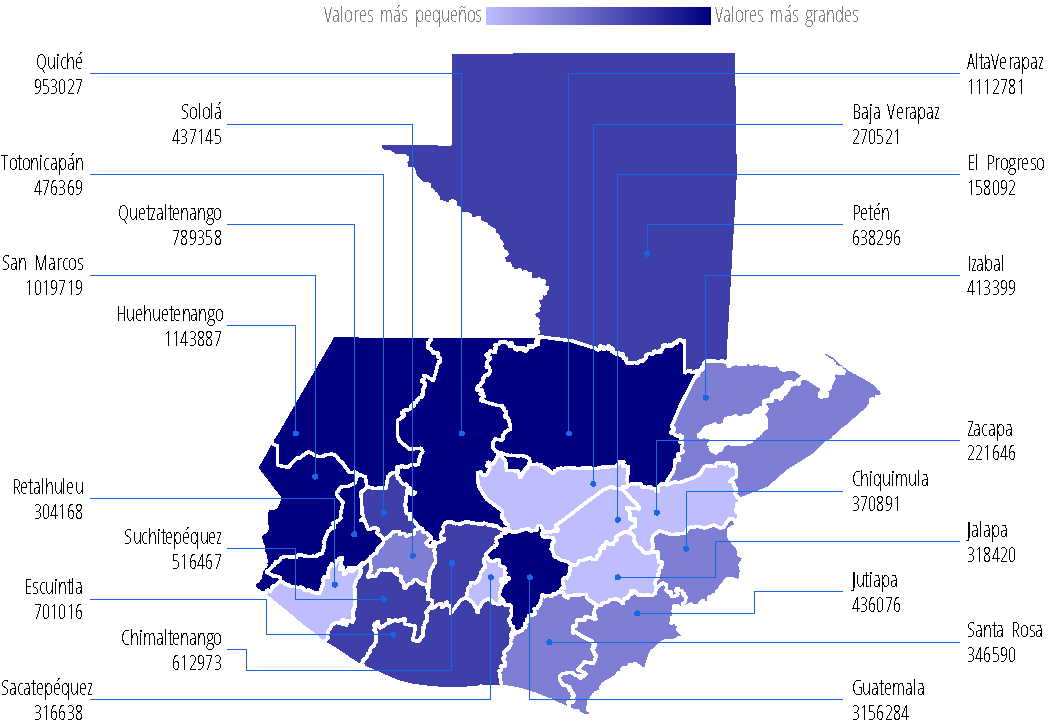
\includegraphics[width=52\cuadri]{graficas/1_02.pdf}}%
  {%
  	Instituto Nacional de Estadística} %
  
  
   %%%%%%%%%%%%%%%%%%%%%%%%%%%%%%%%%%6%%%%%%%%%%%%%%%%%%%%%%%%
   
   
    \cajota{%
    	Población departamental del 2015 }%
    {%
Al igual que en el 2008, los departamentos con la mayor cantidad de habitantes en el 2015 fueron Guatemala, el cual tuvo un crecimiento del , Quetzaltenango, San Marcos, Huehuetenango, Quiché y Alta Verapaz.  }%
    {%
    	Número de habitantes en el 2015 por departamento
    } %
    {%
    	República de Guatemala, por departamentos 2015, en número de habitantes} %
    {%
    	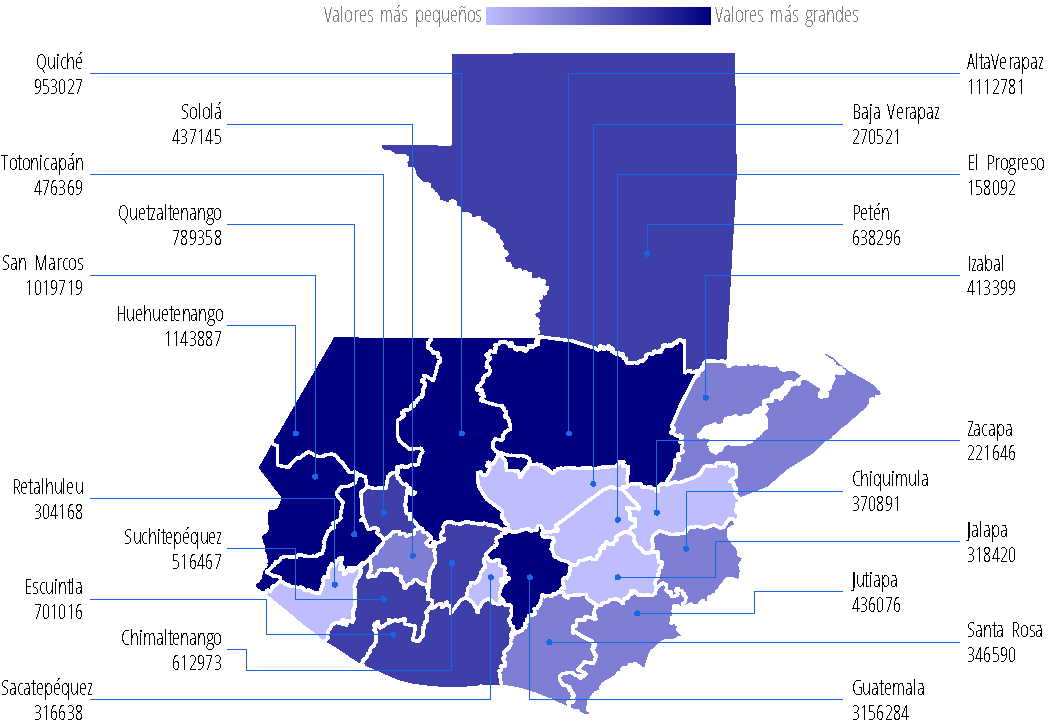
\includegraphics[width=52\cuadri]{graficas/1_02.pdf}}%
    {%
    	Instituto Nacional de Estadística} %
    
    
    %%%%%%%%%%%%%%%%%%%%%%%%%%%%%%%%%%8%%%%%%%%%%%%%%%%%%%%%%%%
    
   \cajota{%
   	Densidad poblacional departamental del 2008 }%
   {%
   }%
   {%
   	Densidad de población en el 2008 por departamento
   } %
   {%
   		República de Guatemala, por departamentos 2008, en número de habitantes por kilómetro cuadrado} %
   {%
   	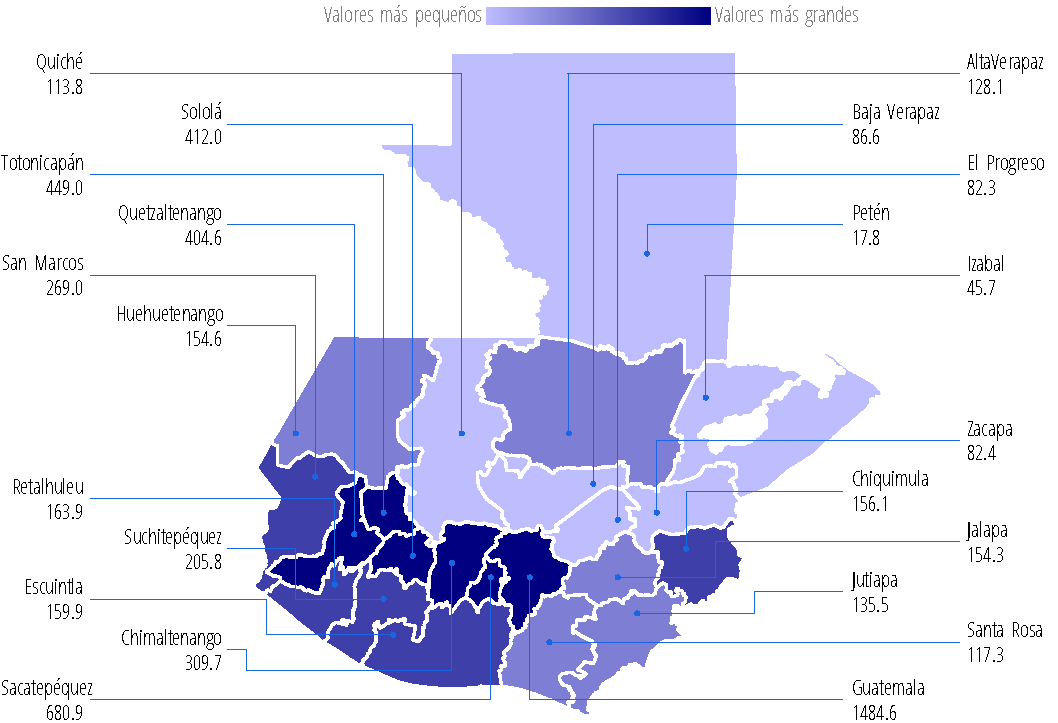
\includegraphics[width=52\cuadri]{graficas/1_05.pdf}}%
   {%
   	Instituto Nacional de Estadística} %
   
   
     %%%%%%%%%%%%%%%%%%%%%%%%%%%%%%%%%%7%%%%%%%%%%%%%%%%%%%%%%%%
     
    
     \cajota{%
     	Densidad poblacional departamental del 2015 }%
     {%
     }%
     {%
     	Densidad de población en el 2015 por departamento
     } %
     {%
     	República de Guatemala, por departamentos 2015, en número de habitantes por kilómetro cuadrado} %
     {%
     	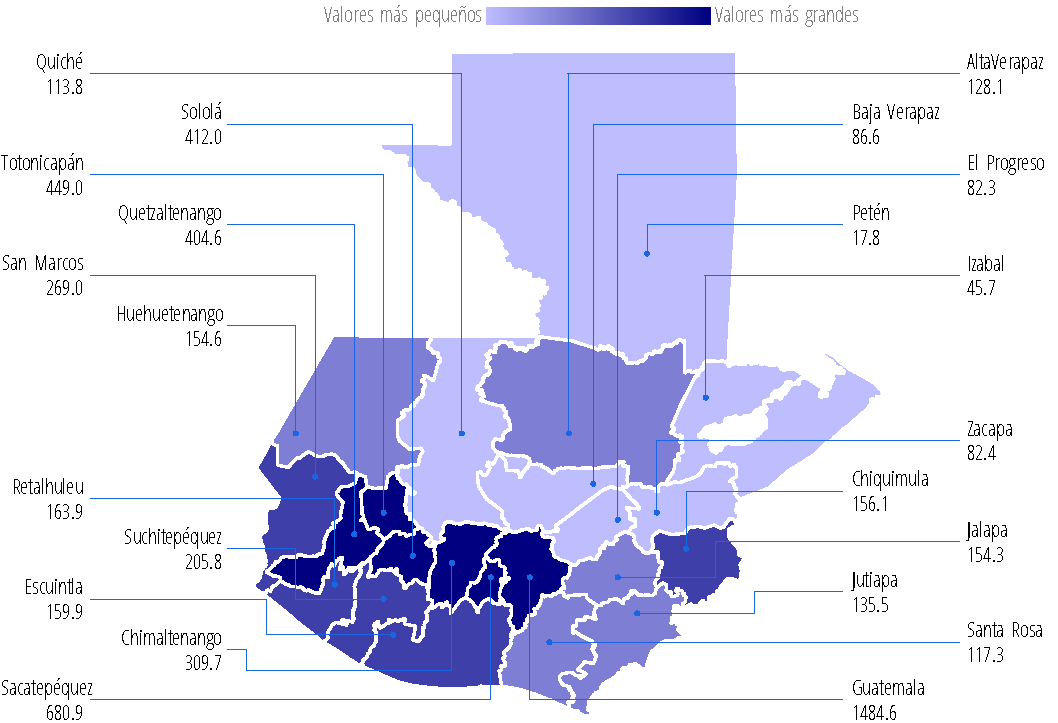
\includegraphics[width=52\cuadri]{graficas/1_05.pdf}}%
     {%
     	Instituto Nacional de Estadística} %

 %%%%%%%%%%%%%%%%%%%%%%%%%%%%%%%%%%9%%%%%%%%%%%%%%%%%%%%%%%%
 
 \cajita{%
 	Índice de desarrollo humano }%
 {%
 El indice de desarrollo humano del 2011, en esencia se mantuvo constante respecto al 2006, con 0.6.\textollamada[*]{Este indicador fue elaborado por el Programa de las Naciones Unidas para el Desarrollo. Esta compuesto por tres parámetros: vida larga y saludable (según la esperanza de vida al nacer), educación (tasa de alfabetización de adultos, tasa bruta combinada de matriculación y años de duración de educación obligatoria.) y nivel de vida digno(medida por el PIB per cápita PPA.)}\textollamada[*]{Este indicador no contempla la desigualdad, pobreza, seguridad humana ni el empoderamiento.} }%
 {%
 	Índice de desarrollo humano y sus componentes} %
 {%
 	República de Guatemala, años 2006 y 2015, adimensional} %
 {%
 	\begin{tikzpicture}[x=1pt,y=1pt]  % Created by tikzDevice version 0.9 on 2016-03-03 01:36:33
% !TEX encoding = UTF-8 Unicode
\definecolor{fillColor}{RGB}{255,255,255}
\path[use as bounding box,fill=fillColor,fill opacity=0.00] (0,0) rectangle (289.08,198.74);
\begin{scope}
\path[clip] (  0.00,  0.00) rectangle (289.08,198.74);

\path[] (  0.00,  0.00) rectangle (289.08,198.74);
\end{scope}
\begin{scope}
\path[clip] (  0.00,  0.00) rectangle (289.08,198.74);

\path[] (  0.00, 18.46) rectangle (289.08,171.32);

\path[] ( 41.30, 18.46) --
	( 41.30,171.32);

\path[] (110.13, 18.46) --
	(110.13,171.32);

\path[] (178.95, 18.46) --
	(178.95,171.32);

\path[] (247.78, 18.46) --
	(247.78,171.32);
\definecolor{drawColor}{RGB}{0,0,255}
\definecolor{fillColor}{RGB}{0,0,255}

\path[draw=drawColor,line width= 0.6pt,line join=round,fill=fillColor] ( 12.05, 18.46) rectangle ( 39.58,124.11);
\definecolor{drawColor}{RGB}{157,187,255}
\definecolor{fillColor}{RGB}{157,187,255}

\path[draw=drawColor,line width= 0.6pt,line join=round,fill=fillColor] ( 43.02, 18.46) rectangle ( 70.55,126.18);
\definecolor{drawColor}{RGB}{0,0,255}
\definecolor{fillColor}{RGB}{0,0,255}

\path[draw=drawColor,line width= 0.6pt,line join=round,fill=fillColor] ( 80.87, 18.46) rectangle (108.40,171.32);
\definecolor{drawColor}{RGB}{157,187,255}
\definecolor{fillColor}{RGB}{157,187,255}

\path[draw=drawColor,line width= 0.6pt,line join=round,fill=fillColor] (111.85, 18.46) rectangle (139.38,168.38);
\definecolor{drawColor}{RGB}{0,0,255}
\definecolor{fillColor}{RGB}{0,0,255}

\path[draw=drawColor,line width= 0.6pt,line join=round,fill=fillColor] (149.70, 18.46) rectangle (177.23, 96.35);
\definecolor{drawColor}{RGB}{157,187,255}
\definecolor{fillColor}{RGB}{157,187,255}

\path[draw=drawColor,line width= 0.6pt,line join=round,fill=fillColor] (180.68, 18.46) rectangle (208.21,102.44);
\definecolor{drawColor}{RGB}{0,0,255}
\definecolor{fillColor}{RGB}{0,0,255}

\path[draw=drawColor,line width= 0.6pt,line join=round,fill=fillColor] (218.53, 18.46) rectangle (246.06,117.51);
\definecolor{drawColor}{RGB}{157,187,255}
\definecolor{fillColor}{RGB}{157,187,255}

\path[draw=drawColor,line width= 0.6pt,line join=round,fill=fillColor] (249.50, 18.46) rectangle (277.03,117.72);
\definecolor{drawColor}{RGB}{0,0,0}

\path[draw=drawColor,line width= 0.6pt,line join=round] (  0.00, 18.46) -- (289.08, 18.46);

\node[text=drawColor,rotate= 90.00,anchor=base west,inner sep=0pt, outer sep=0pt, scale=  0.83] at ( 29.05,125.94) {0.6};

\node[text=drawColor,rotate= 90.00,anchor=base west,inner sep=0pt, outer sep=0pt, scale=  0.83] at ( 60.02,128.00) {0.6};

\node[text=drawColor,rotate= 90.00,anchor=base west,inner sep=0pt, outer sep=0pt, scale=  0.83] at ( 97.87,173.15) {0.8};

\node[text=drawColor,rotate= 90.00,anchor=base west,inner sep=0pt, outer sep=0pt, scale=  0.83] at (128.85,170.21) {0.8};

\node[text=drawColor,rotate= 90.00,anchor=base west,inner sep=0pt, outer sep=0pt, scale=  0.83] at (166.70, 98.18) {0.4};

\node[text=drawColor,rotate= 90.00,anchor=base west,inner sep=0pt, outer sep=0pt, scale=  0.83] at (197.68,104.27) {0.5};

\node[text=drawColor,rotate= 90.00,anchor=base west,inner sep=0pt, outer sep=0pt, scale=  0.83] at (235.53,119.33) {0.5};

\node[text=drawColor,rotate= 90.00,anchor=base west,inner sep=0pt, outer sep=0pt, scale=  0.83] at (266.50,119.54) {0.5};

\path[] (  0.00, 18.46) rectangle (289.08,171.32);
\end{scope}
\begin{scope}
\path[clip] (  0.00,  0.00) rectangle (289.08,198.74);

\path[] (  0.00, 18.46) --
	(289.08, 18.46);
\end{scope}
\begin{scope}
\path[clip] (  0.00,  0.00) rectangle (289.08,198.74);

\path[] ( 41.30, 15.71) --
	( 41.30, 18.46);

\path[] (110.13, 15.71) --
	(110.13, 18.46);

\path[] (178.95, 15.71) --
	(178.95, 18.46);

\path[] (247.78, 15.71) --
	(247.78, 18.46);
\end{scope}
\begin{scope}
\path[clip] (  0.00,  0.00) rectangle (289.08,198.74);
\definecolor{drawColor}{RGB}{0,0,0}

\node[text=drawColor,anchor=base,inner sep=0pt, outer sep=0pt, scale=  1.00] at ( 41.30,  5.69) {IDH};

\node[text=drawColor,anchor=base,inner sep=0pt, outer sep=0pt, scale=  1.00] at (110.13,  5.69) {IDH Salud};

\node[text=drawColor,anchor=base,inner sep=0pt, outer sep=0pt, scale=  1.00] at (178.95,  5.69) {IDH Educación};

\node[text=drawColor,anchor=base,inner sep=0pt, outer sep=0pt, scale=  1.00] at (247.78,  5.69) {IDH Ingresos};
\end{scope}
\begin{scope}
\path[clip] (  0.00,  0.00) rectangle (289.08,198.74);
\coordinate (apoyo) at (61.19,191.48);
\coordinate (longitudFicticia) at (7.11,7.26);
\coordinate (longitud) at (7.11,7.11);
\coordinate (desX) at (138.78,0);
\coordinate (desY) at (0,0.07);
\definecolor[named]{ct1}{HTML}{
0000FF
}
\definecolor[named]{ct2}{HTML}{
9DBBFF
}
\definecolor[named]{ctb1}{HTML}{
0000FF
}
\definecolor[named]{ctb2}{HTML}{
9DBBFF
}
\path [fill=none] (apoyo) rectangle ($(apoyo)+(longitudFicticia)$)
node [xshift=0.3cm,inner sep=0pt, outer sep=0pt,midway,right,scale = 0.9]{2006};
\draw [color = ctb1,fill=ct1] ( $(apoyo)  + (desY) $) rectangle ($(apoyo)+ (desY) +(longitud)$);
\path [fill=none] ($(apoyo)+(desX)$) rectangle ($(apoyo)+(desX)+(longitudFicticia)$)
node [xshift=0.3cm,inner sep=0pt, outer sep=0pt,midway,right,scale = 0.9]{2011};
\draw [color = ctb2 ,fill=ct2] ( $(apoyo)  + (desY) + (desX) $) rectangle ($(apoyo)+ (desY)+ (desX) +(longitud)$);
\end{scope}
  \end{tikzpicture}}%
 {%
 	Informe Nacional de Desarrollo Humano (PNUD), con base en las Encuestas Nacionales de Condiciones de Vida (Encovi).} % 
   
   
   
   %%%%%%%%%%%%%%%%%%%%%%%%%%%%%%%%%%10%%%%%%%%%%%%%%%%%%%%%%%%
   
   \cajota{%
   	IDH en los departamentos}%
   	{%
 Según el índice de desarrollo humano calculado para cada departamento, Guatemala está por arriba del IDH nacional.
 Los departamentos de Quiché, Sololá, Totonicapán, San Marcos, Huehuetenango, Retalhuleu, Suchitepéquez, Santa Rosa, Chiquimula, Jalapa, Petén y Alta Verapaz están por debajo del IDH nacional de 0.6. 	}%
   	{%
   		Índice de desarrollo humano
   	}%
   	{%
   	Por departamento, año 2015, adimensional} %
   	{%
   		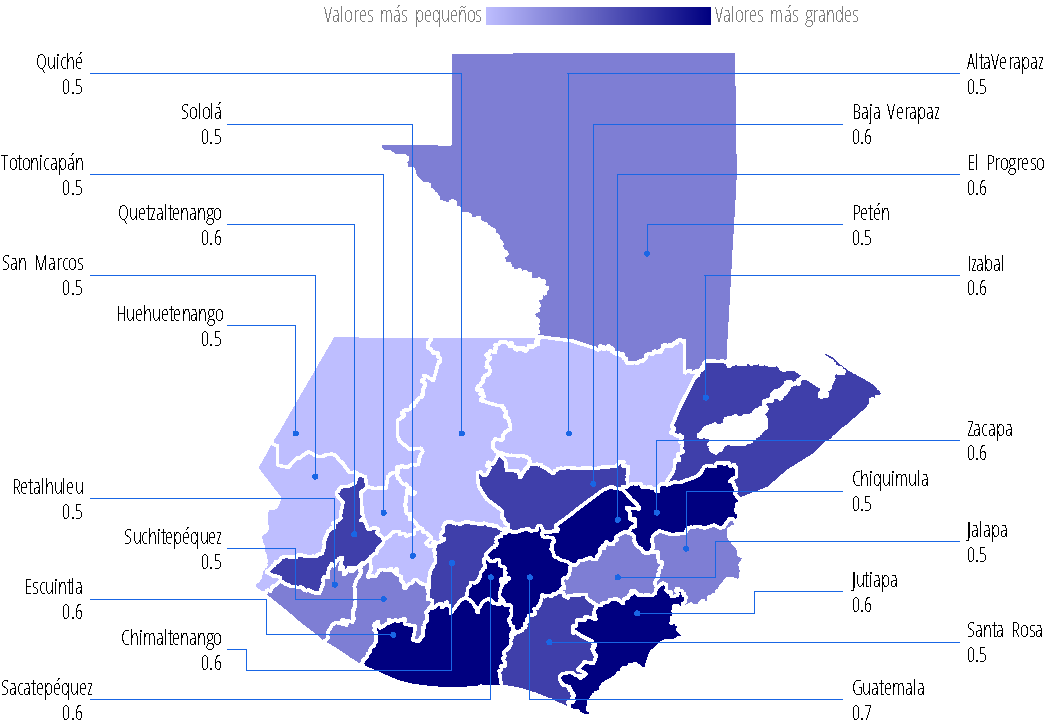
\includegraphics[width=52\cuadri]{graficas/1_11.pdf}}%
   	{%
   		Instituto Nacional de Estadística} %
 
 
 
 
      %%%%%%%%%%%%%%%%%%%%%%%%%%%%%%%%%%11%%%%%%%%%%%%%%%%%%%%%%%%
      
      \cajota{%
      	Calidad de la vivienda en los departamentos}%
      {%
   Se incluyen las variables de la ENCOVI 2014 asociadas con los materiales de construcción utilizados en el piso, paredes y techo. 
   
   Los departamentos que en el 2014 más de la mitad de los hogares tenían esta necesidad básica insatisfecha fueron Alta Verapaz (77.2\%), Jalapa (70.1\%), Chiquimula (60.6\%),Huehuetenango (56.2\%), Totonicapán (59.0\%), Petén (54.4\%) e Izabal (53.6\%). \textollamada[*]{Es un método directo para identificar carencias críticas en una población y caracterizar la pobreza. Toma datos disponibles de los censos de población y encuestas de condiciones de vida. La fuente más reciente de esta información es la Encuesta Nacional de Condiciones de Vida 2014.} }%
      {%
      	Necesidad básica insatisfecha: vivienda
      } %
      {%
      	Por departamento, año 2014, en porcentaje} %
      {%
      	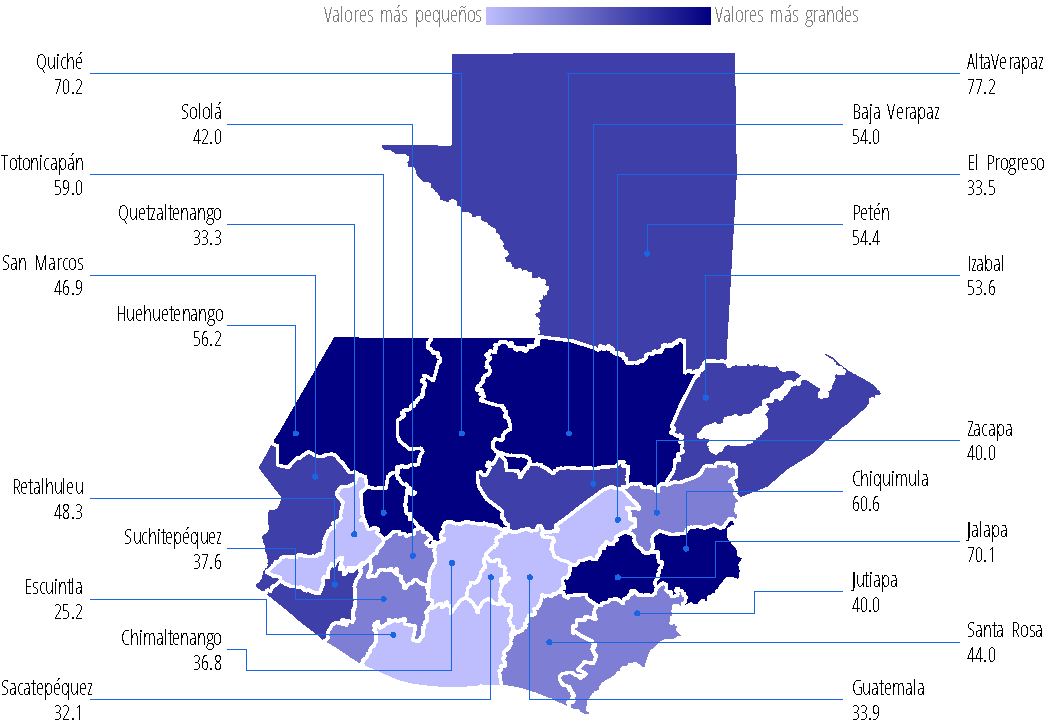
\includegraphics[width=52\cuadri]{graficas/1_12.pdf}}%
      {%
      	Instituto Nacional de Estadística} %
      
      
        %%%%%%%%%%%%%%%%%%%%%%%%%%%%%%%%%%12%%%%%%%%%%%%%%%%%%%%%%%%
        
        \cajota{%
        	Hogares que viven en hacinamiento}%
        {% 
        El hacinamiento toma las variables de la Encuesta Nacional de Condiciones de Vida que recogen información sobre el número de personas en el hogar y el número de cuartos de la vivienda.
        
        Los departamentos con mayor porcentaje de hogares que vivían en hacinamiento fueron Alta Verapaz (64.8\%), Quiché (59.9\%), Huehuetenango (54.6\%), Suchitepéquez (52.8\%), Izabal (52.5\%), Petén (51.4\%), Jalapa (51.4\%) }%
        {%
        	Hogares en hacinamiento
        } %
        {%
        	Por departamento, año 2014, en porcentaje} %
        {%
        	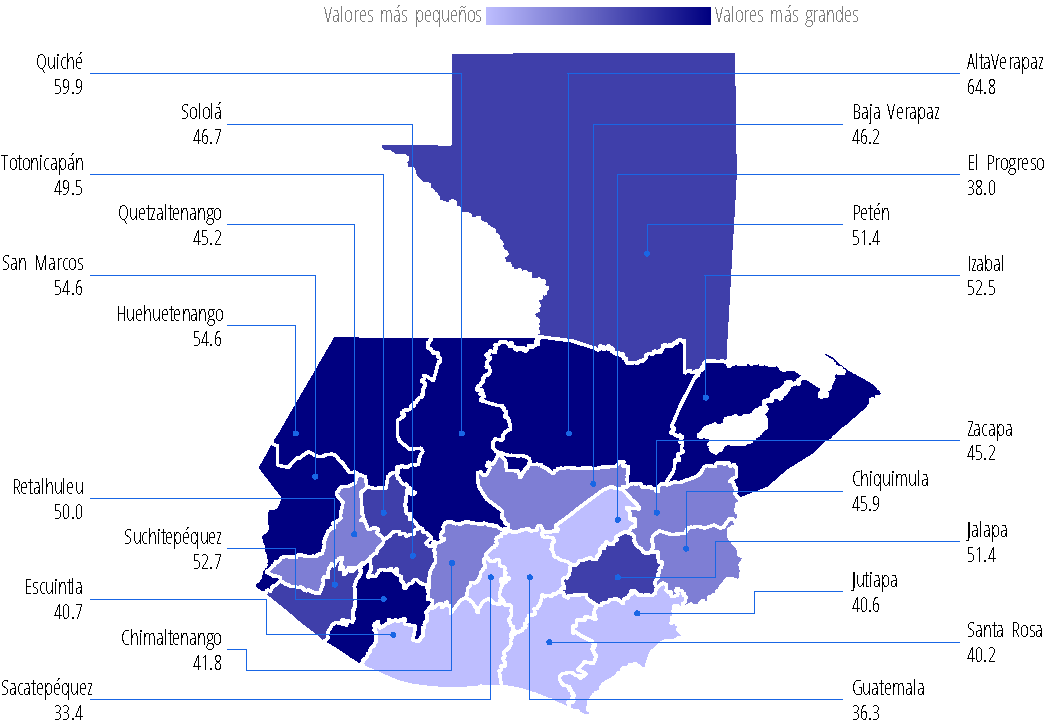
\includegraphics[width=52\cuadri]{graficas/1_13.pdf}}%
        {%
        	Instituto Nacional de Estadística} %
        
        
          
          %%%%%%%%%%%%%%%%%%%%%%%%%%%%%%%%%%13%%%%%%%%%%%%%%%%%%%%%%%%
          
          \cajota{%
          	Acceso a agua}%
          {%
         El acceso y/o disponibilidad de agua potable se encuentra en las necesidades básicas de acceso a servicios sanitarios.  Se toma de las variables de la ENCOVI 2014 que recogen información sobre la fuente de abastecimiento de agua en la vivienda.
         
         Para el 2014 el departamento de Alta Verapaz en más del 50\% de hogares esta necesidad básica estaba insatisfecha. }%
          {%
          	Hogares que no poseen acceso a agua entubada
          } %
          {%
          	República de Guatemala, por departamentos, en porcentaje} %
          {%
          	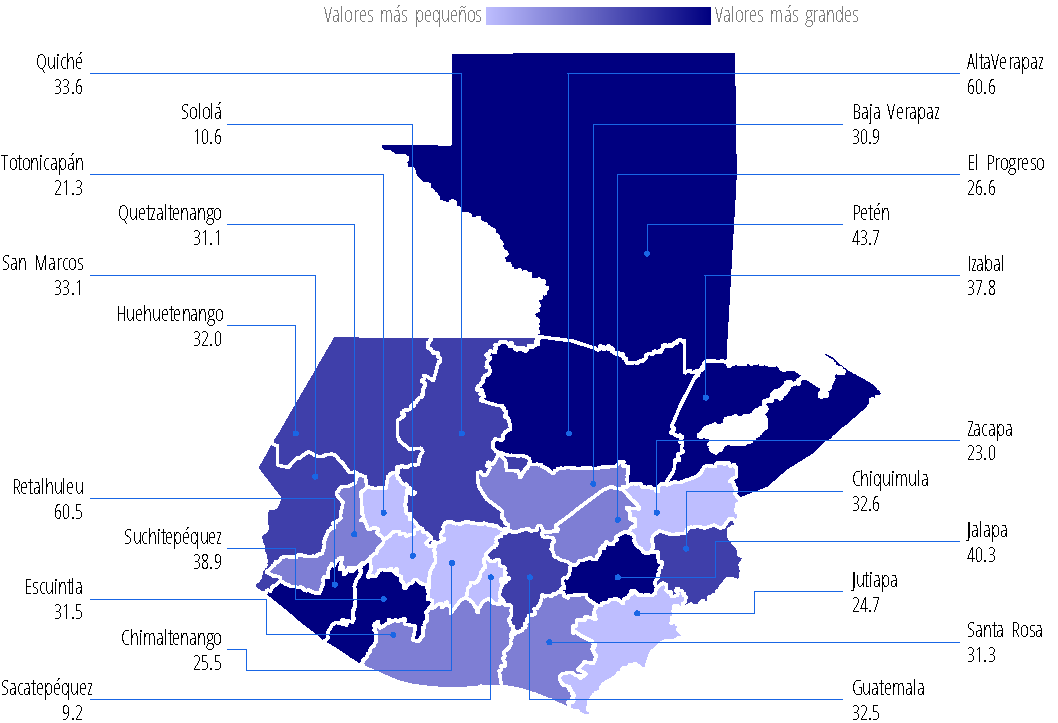
\includegraphics[width=52\cuadri]{graficas/1_14.pdf}}%
          {%
          	Instituto Nacional de Estadística} %
          
          
                    %%%%%%%%%%%%%%%%%%%%%%%%%%%%%%%%%%14%%%%%%%%%%%%%%%%%%%%%%%%
                    
                    \cajota{%
                    Acceso a servicios de saneamiento}%
                    {%
Esta necesidad básica, clasificada en el acceso a servicios sanitarios, tomas las variables de la Encuesta Nacional de Condiciones de Vida que recoge las variables sobre disponibilidad de servicio sanitario y sistema de eliminación de excretas.

Para el 2014, los departamentos donde 3 de cada 10 hogares no contaban con esta necesidad satisfecha fueron Chiquimula, Jalapa, Petén y Jutiapa.   }%
                    {%
                    	Hogares sin acceso a servicios de saneamiento }
                    {%
                    	Por departamento, año 2014, en porcentaje} %
                    {%
                    	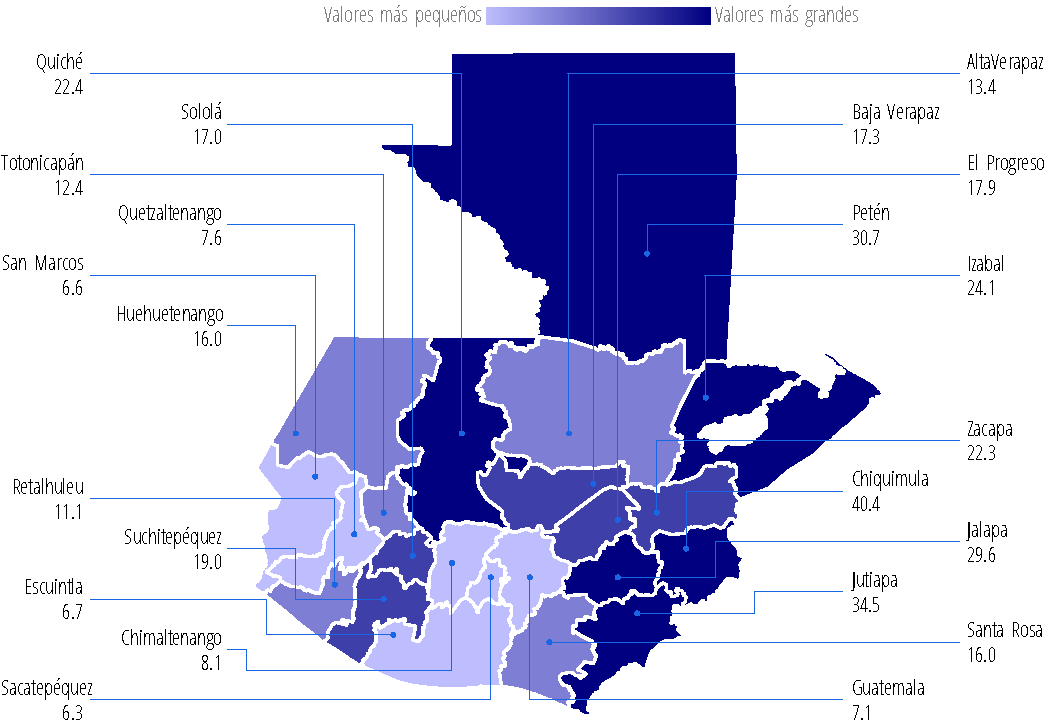
\includegraphics[width=52\cuadri]{graficas/1_15.pdf}}%
                    {%
                    	Instituto Nacional de Estadística} %

                  
                     %%%%%%%%%%%%%%%%%%%%%%%%%%%%%%%%%%18%%%%%%%%%%%%%%%%%%%%%%%%
                     
                     \cajota{%
                     	Pobreza total }%
                     {%
                  Según la Encuesta Nacional de Condiciones de Vida 2014, los departamentos con mayor incidencia de pobreza (que incluye la pobreza extrema y la no extrema) fueron Alta Verapaz con el 83.1\%, Sololá con 80.9\%, Totonicapán 77.5\% y Quiché con 74.7\%. }%
                     {%
                     	Pobreza total
                     } %
                     {%
                     Por departamento, año 2014, en porcentaje} %
                     {%
                     	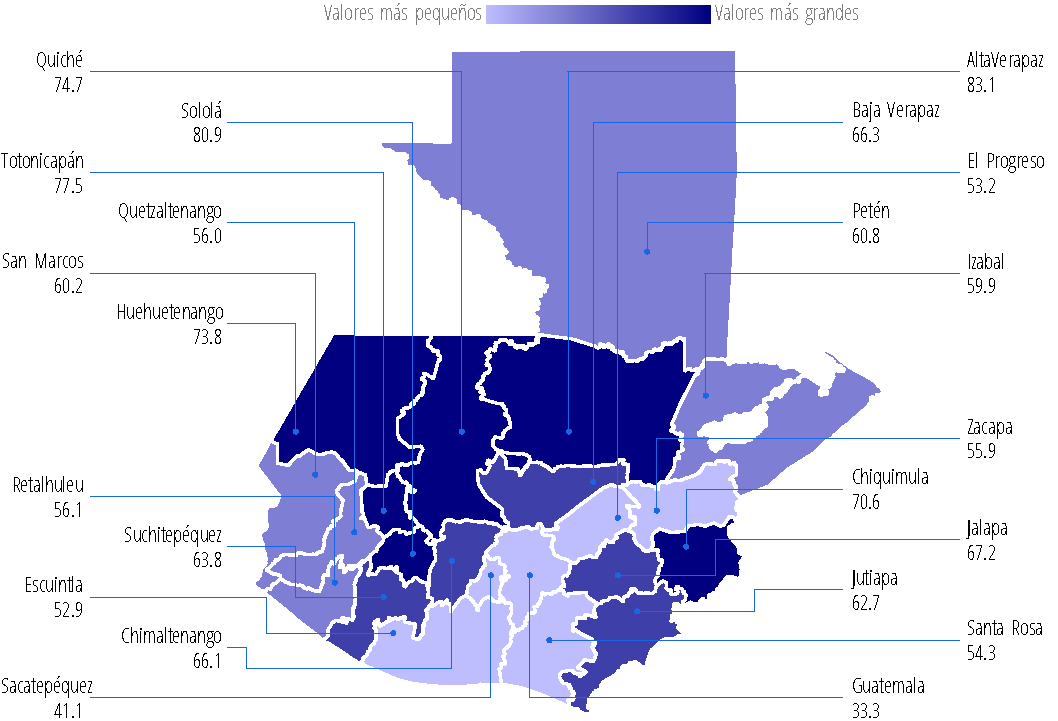
\includegraphics[width=52\cuadri]{graficas/1_19.pdf}}%
                     {%
                     	INE, ENCOVI 2014} %
                     
                    %%%%%%%%%%%%%%%%%%%%%%%%%%%%%%%%%%16%%%%%%%%%%%%%%%%%%%%%%%%
                    
                    \cajota{%
                    	Pobreza total rural}%
                    {%
                    Los departamentos donde 8 de cada 10 personas que habitaban en áreas rurales estaban en condiciones de pobreza (extremo o no extremo) fueron Alta Verapaz, Quiché, Totonicapán y Sololá}%
                    {%
                    	Pobreza total rural por departamentos
                    } %
                    {%
                    	República de Guatemala, por departamentos año 2014, en porcentaje} %
                    {%
                    	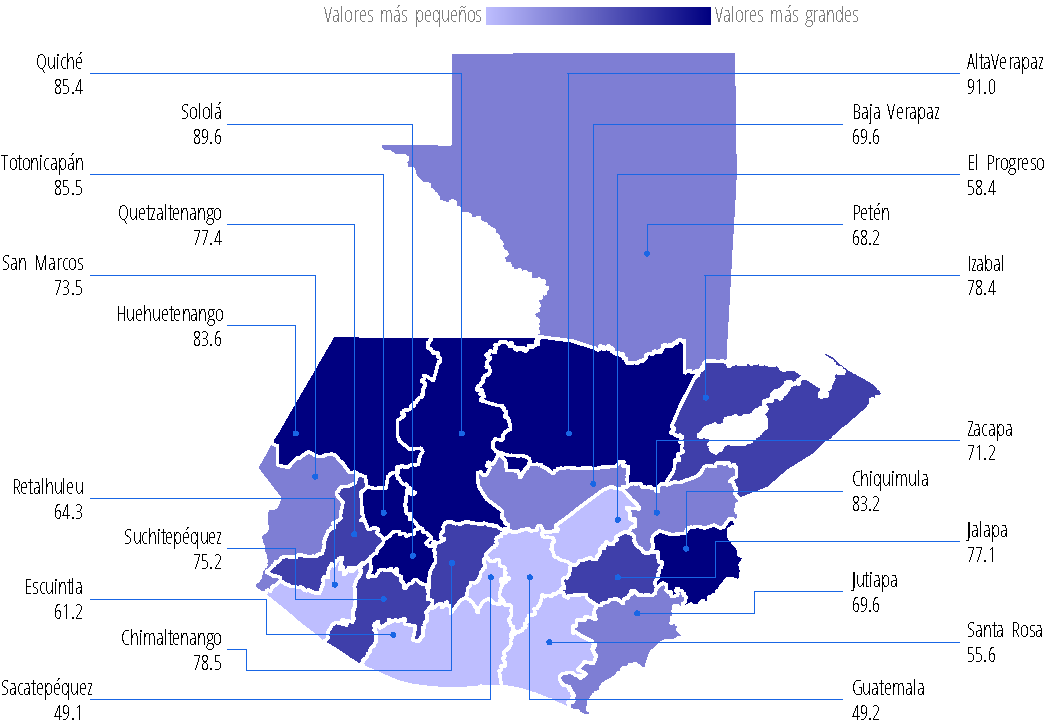
\includegraphics[width=52\cuadri]{graficas/1_17.pdf}}%
                    {%
                    	INE, ENCOVI 2014} %
                    %%%%%%%%%%%%%%%%%%%%%%%%%%%%%%%%%%17%%%%%%%%%%%%%%%%%%%%%%%%
                    
                    \cajota{%
                    	Pobreza extrema }%
                    {%
                   La pobreza extrema a nivel departamental  }%
                    {%
                    El departamento con la mayor incidencia de pobreza extrema fue Alta Verapaz (53.6\%).
                    } %
                    {%
                    	República de Guatemala, por departamentos año 2014, en porcentaje} %
                    {%
                    	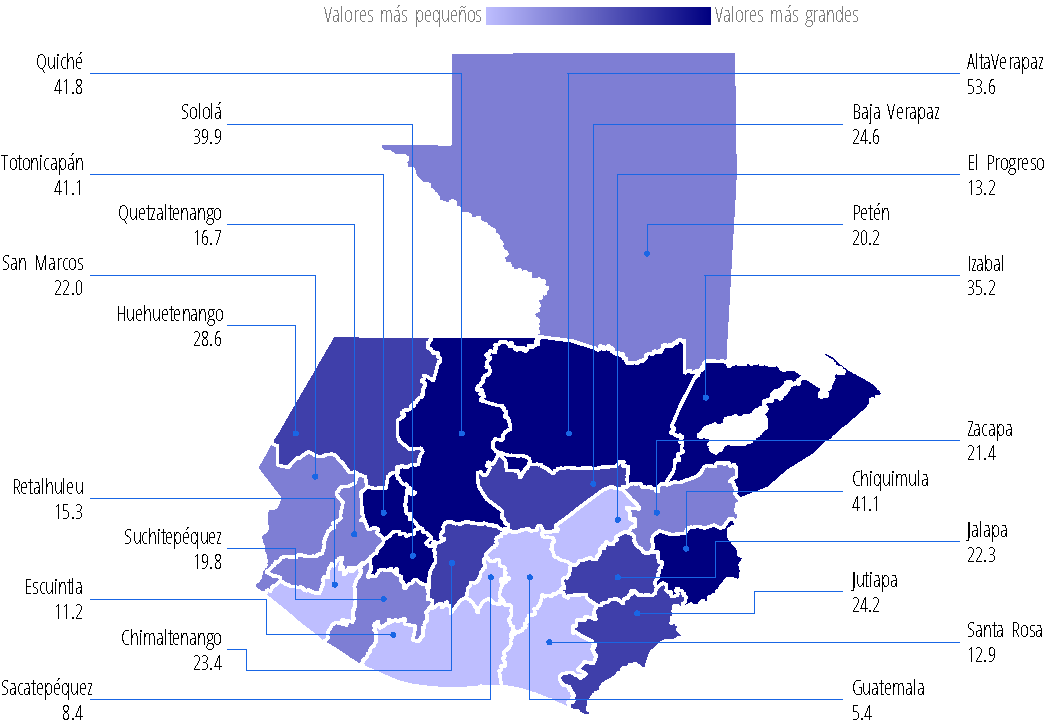
\includegraphics[width=52\cuadri]{graficas/1_18.pdf}}%
                    {%
                    	INE, ENCOVI 2014} %
                    
                     %%%%%%%%%%%%%%%%%%%%%%%%%%%%%%%%%%15%%%%%%%%%%%%%%%%%%%%%%%%
                     
                     \cajota{%
                     	Pobreza extrema rural}%
                     {%
                     	El análisis de las personas que habitan en áreas rurales y desagregarlos según su nivel de pobreza, muestra que el 50.4\% de los habitantes en áreas rurales en Sololá estaban debajo de la línea de pobreza extrema, así también Izabal (52.1\%), 52.9\% en Totonicapán, 54.2\% en Chiquimula, 57.9\% en Alta Verapaz, que fueron los departamentos con mayor incidencia en el 2014.
                     	
                     	En Alta Verapaz la incidencia de pobreza extrema en las áreas rurales es mayor que la incidencia departamental en 4.3 puntos porcentuales.}%
                     {%
                     	Pobreza extrema rural por departamentos
                     } %
                     {%
                     	Por departamento, año 2014, en porcentaje} %
                     {%
                     	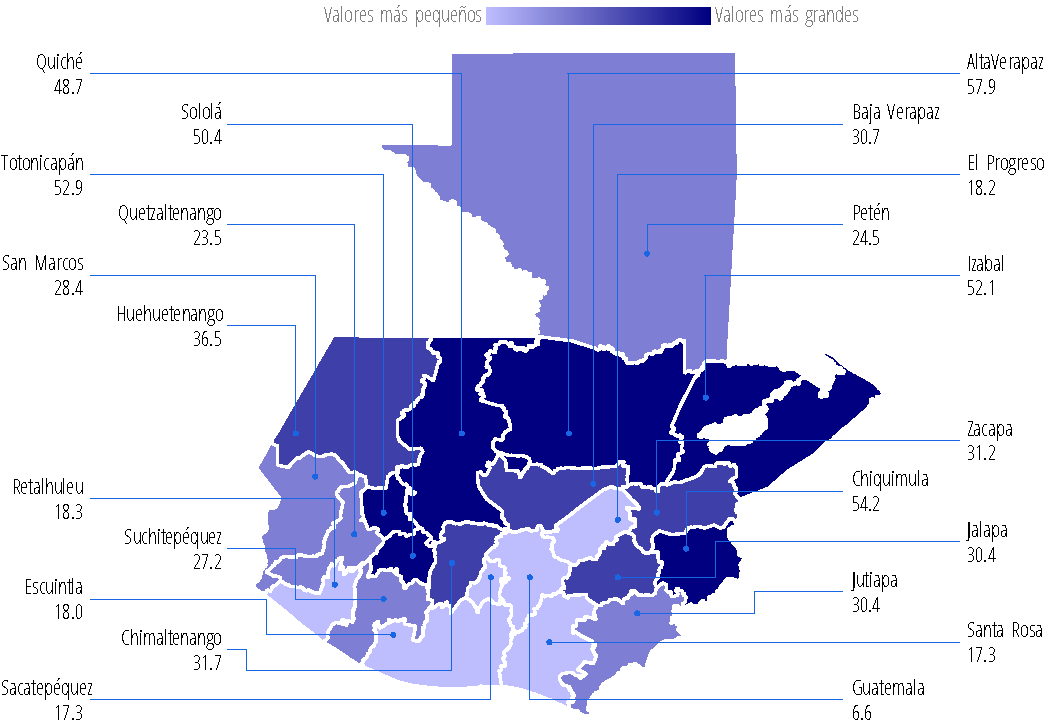
\includegraphics[width=52\cuadri]{graficas/1_16.pdf}}%
                     {%
                     	INE, ENCOVI 2014} %
         
 %%%%%%%%%%%%%%%%%%%%%%%%%%%%%%%%%%19%%%%%%%%%%%%%%%%%%%%%%%%
 
 \cajita{%
 	PET }%
 {%
 }%
 {%
 	Población en edad de trabajar} %
 {%
 	República de Guatemala, serie histórica por ENEI, en número de personas} %
 {%
 	\begin{tikzpicture}[x=1pt,y=1pt]  % Created by tikzDevice version 0.9 on 2016-03-03 00:54:40
% !TEX encoding = UTF-8 Unicode
\definecolor{fillColor}{RGB}{255,255,255}
\path[use as bounding box,fill=fillColor,fill opacity=0.00] (0,0) rectangle (289.08,198.74);
\begin{scope}
\path[clip] (  0.00,  0.00) rectangle (289.08,198.74);

\path[] (  0.00,  0.00) rectangle (289.08,198.74);
\end{scope}
\begin{scope}
\path[clip] (  0.00,  0.00) rectangle (289.08,198.74);

\path[] ( 25.76, 15.61) rectangle (280.54,191.48);

\path[] ( 25.76, 31.48) --
	(280.54, 31.48);

\path[] ( 25.76, 74.96) --
	(280.54, 74.96);

\path[] ( 25.76,118.43) --
	(280.54,118.43);

\path[] ( 25.76,161.90) --
	(280.54,161.90);

\path[] ( 25.76, 53.22) --
	(280.54, 53.22);

\path[] ( 25.76, 96.69) --
	(280.54, 96.69);

\path[] ( 25.76,140.16) --
	(280.54,140.16);

\path[] ( 25.76,183.64) --
	(280.54,183.64);

\path[] ( 62.15, 15.61) --
	( 62.15,191.48);

\path[] (122.82, 15.61) --
	(122.82,191.48);

\path[] (183.48, 15.61) --
	(183.48,191.48);

\path[] (244.15, 15.61) --
	(244.15,191.48);
\definecolor{drawColor}{RGB}{0,0,255}

\path[draw=drawColor,line width= 1.7pt,line join=round] ( 62.15, 60.50) --
	(122.82, 99.42) --
	(183.48,131.03) --
	(244.15,183.49);
\definecolor{drawColor}{RGB}{0,0,0}

\node[text=drawColor,anchor=base,inner sep=0pt, outer sep=0pt, scale=  1.02] at ( 62.15, 48.59) {9,083,763};

\node[text=drawColor,anchor=base east,inner sep=0pt, outer sep=0pt, scale=  1.02] at (115.67, 99.42) {9,531,370};

\node[text=drawColor,anchor=base east,inner sep=0pt, outer sep=0pt, scale=  1.02] at (176.34,131.03) {9,894,951};

\node[text=drawColor,anchor=base,inner sep=0pt, outer sep=0pt, scale=  1.02] at (244.15,187.46) {10,498,289};

\path[draw=drawColor,line width= 0.1pt,line join=round] ( 25.76, 23.61) -- (280.54, 23.61);

\path[] ( 25.76, 15.61) rectangle (280.54,191.48);
\end{scope}
\begin{scope}
\path[clip] (  0.00,  0.00) rectangle (289.08,198.74);

\path[] ( 25.76, 15.61) --
	( 25.76,191.48);
\end{scope}
\begin{scope}
\path[clip] (  0.00,  0.00) rectangle (289.08,198.74);
\definecolor{drawColor}{RGB}{255,255,255}

\node[text=drawColor,text opacity=0.00,anchor=base east,inner sep=0pt, outer sep=0pt, scale=  1.00] at ( 20.81, 49.31) {9000000};

\node[text=drawColor,text opacity=0.00,anchor=base east,inner sep=0pt, outer sep=0pt, scale=  1.00] at ( 20.81, 92.78) {9500000};

\node[text=drawColor,text opacity=0.00,anchor=base east,inner sep=0pt, outer sep=0pt, scale=  1.00] at ( 20.81,136.26) {10000000};

\node[text=drawColor,text opacity=0.00,anchor=base east,inner sep=0pt, outer sep=0pt, scale=  1.00] at ( 20.81,179.73) {10500000};
\end{scope}
\begin{scope}
\path[clip] (  0.00,  0.00) rectangle (289.08,198.74);

\path[] ( 23.01, 53.22) --
	( 25.76, 53.22);

\path[] ( 23.01, 96.69) --
	( 25.76, 96.69);

\path[] ( 23.01,140.16) --
	( 25.76,140.16);

\path[] ( 23.01,183.64) --
	( 25.76,183.64);
\end{scope}
\begin{scope}
\path[clip] (  0.00,  0.00) rectangle (289.08,198.74);

\path[] ( 25.76, 15.61) --
	(280.54, 15.61);
\end{scope}
\begin{scope}
\path[clip] (  0.00,  0.00) rectangle (289.08,198.74);

\path[] ( 62.15, 12.86) --
	( 62.15, 15.61);

\path[] (122.82, 12.86) --
	(122.82, 15.61);

\path[] (183.48, 12.86) --
	(183.48, 15.61);

\path[] (244.15, 12.86) --
	(244.15, 15.61);
\end{scope}
\begin{scope}
\path[clip] (  0.00,  0.00) rectangle (289.08,198.74);
\definecolor{drawColor}{RGB}{0,0,0}

\node[text=drawColor,anchor=base,inner sep=0pt, outer sep=0pt, scale=  1.00] at ( 62.15,  2.85) {2011};

\node[text=drawColor,anchor=base,inner sep=0pt, outer sep=0pt, scale=  1.00] at (122.82,  2.85) {2012};

\node[text=drawColor,anchor=base,inner sep=0pt, outer sep=0pt, scale=  1.00] at (183.48,  2.85) {2013};

\node[text=drawColor,anchor=base,inner sep=0pt, outer sep=0pt, scale=  1.00] at (244.15,  2.85) {2014};
\end{scope}
  \end{tikzpicture}}%
 {%
 	ENEI 2014, 2013, 2012 y 2011} % 
 
 
  %%%%%%%%%%%%%%%%%%%%%%%%%%%%%%%%%%20%%%%%%%%%%%%%%%%%%%%%%%%
 
 \cajita{%
 	PEA }%
 {%
 }%
 {%
 	Población económicamente activa} %
 {%
 	República de Guatemala, serie histórica por ENEI, en número de personas} %
 {%
 	\begin{tikzpicture}[x=1pt,y=1pt]  % Created by tikzDevice version 0.9 on 2016-03-03 02:00:13
% !TEX encoding = UTF-8 Unicode
\definecolor{fillColor}{RGB}{255,255,255}
\path[use as bounding box,fill=fillColor,fill opacity=0.00] (0,0) rectangle (289.08,198.74);
\begin{scope}
\path[clip] (  0.00,  0.00) rectangle (289.08,198.74);

\path[] (  0.00,  0.00) rectangle (289.08,198.74);
\end{scope}
\begin{scope}
\path[clip] (  0.00,  0.00) rectangle (289.08,198.74);

\path[] ( 21.38, 15.61) rectangle (280.54,191.48);

\path[] ( 21.38, 26.79) --
	(280.54, 26.79);

\path[] ( 21.38, 68.42) --
	(280.54, 68.42);

\path[] ( 21.38,110.05) --
	(280.54,110.05);

\path[] ( 21.38,151.68) --
	(280.54,151.68);

\path[] ( 21.38, 47.60) --
	(280.54, 47.60);

\path[] ( 21.38, 89.23) --
	(280.54, 89.23);

\path[] ( 21.38,130.87) --
	(280.54,130.87);

\path[] ( 21.38,172.50) --
	(280.54,172.50);

\path[] ( 58.40, 15.61) --
	( 58.40,191.48);

\path[] (120.11, 15.61) --
	(120.11,191.48);

\path[] (181.81, 15.61) --
	(181.81,191.48);

\path[] (243.52, 15.61) --
	(243.52,191.48);
\definecolor{drawColor}{RGB}{0,0,255}

\path[draw=drawColor,line width= 1.7pt,line join=round] ( 58.40, 60.50) --
	(120.11,170.01) --
	(181.81,129.27) --
	(243.52,183.49);
\definecolor{drawColor}{RGB}{0,0,0}

\node[text=drawColor,anchor=base,inner sep=0pt, outer sep=0pt, scale=  1.02] at ( 58.40, 48.59) {5,577,471};

\node[text=drawColor,anchor=base,inner sep=0pt, outer sep=0pt, scale=  1.02] at (120.11,173.98) {6,235,064};

\node[text=drawColor,anchor=base,inner sep=0pt, outer sep=0pt, scale=  1.02] at (181.81,117.36) {5,990,436};

\node[text=drawColor,anchor=base,inner sep=0pt, outer sep=0pt, scale=  1.02] at (243.52,187.46) {6,316,005};

\path[draw=drawColor,line width= 0.1pt,line join=round] ( 21.38, 23.61) -- (280.54, 23.61);

\path[] ( 21.38, 15.61) rectangle (280.54,191.48);
\end{scope}
\begin{scope}
\path[clip] (  0.00,  0.00) rectangle (289.08,198.74);

\path[] ( 21.38, 15.61) --
	( 21.38,191.48);
\end{scope}
\begin{scope}
\path[clip] (  0.00,  0.00) rectangle (289.08,198.74);
\definecolor{drawColor}{RGB}{255,255,255}

\node[text=drawColor,text opacity=0.00,anchor=base east,inner sep=0pt, outer sep=0pt, scale=  1.00] at ( 16.43, 43.69) {5500000};

\node[text=drawColor,text opacity=0.00,anchor=base east,inner sep=0pt, outer sep=0pt, scale=  1.00] at ( 16.43, 85.32) {5750000};

\node[text=drawColor,text opacity=0.00,anchor=base east,inner sep=0pt, outer sep=0pt, scale=  1.00] at ( 16.43,126.96) {6000000};

\node[text=drawColor,text opacity=0.00,anchor=base east,inner sep=0pt, outer sep=0pt, scale=  1.00] at ( 16.43,168.59) {6250000};
\end{scope}
\begin{scope}
\path[clip] (  0.00,  0.00) rectangle (289.08,198.74);

\path[] ( 18.63, 47.60) --
	( 21.38, 47.60);

\path[] ( 18.63, 89.23) --
	( 21.38, 89.23);

\path[] ( 18.63,130.87) --
	( 21.38,130.87);

\path[] ( 18.63,172.50) --
	( 21.38,172.50);
\end{scope}
\begin{scope}
\path[clip] (  0.00,  0.00) rectangle (289.08,198.74);

\path[] ( 21.38, 15.61) --
	(280.54, 15.61);
\end{scope}
\begin{scope}
\path[clip] (  0.00,  0.00) rectangle (289.08,198.74);

\path[] ( 58.40, 12.86) --
	( 58.40, 15.61);

\path[] (120.11, 12.86) --
	(120.11, 15.61);

\path[] (181.81, 12.86) --
	(181.81, 15.61);

\path[] (243.52, 12.86) --
	(243.52, 15.61);
\end{scope}
\begin{scope}
\path[clip] (  0.00,  0.00) rectangle (289.08,198.74);
\definecolor{drawColor}{RGB}{0,0,0}

\node[text=drawColor,anchor=base,inner sep=0pt, outer sep=0pt, scale=  1.00] at ( 58.40,  2.85) {2011};

\node[text=drawColor,anchor=base,inner sep=0pt, outer sep=0pt, scale=  1.00] at (120.11,  2.85) {2012};

\node[text=drawColor,anchor=base,inner sep=0pt, outer sep=0pt, scale=  1.00] at (181.81,  2.85) {2013};

\node[text=drawColor,anchor=base,inner sep=0pt, outer sep=0pt, scale=  1.00] at (243.52,  2.85) {2014};
\end{scope}
  \end{tikzpicture}}%
 {%
 	ENEI 2014, 2013, 2012 y 2011} % 
 
 
  %%%%%%%%%%%%%%%%%%%%%%%%%%%%%%%%%%21%%%%%%%%%%%%%%%%%%%%%%%%
  
  \cajita{%
  	Población ocupada }%
  {%
  }%
  {%
  	Población ocupada a nivel nacional} %
  {%
  	República de Guatemala, serie histórica por ENEI, en número de personas} %
  {%
  	\begin{tikzpicture}[x=1pt,y=1pt]  % Created by tikzDevice version 0.9 on 2016-03-03 02:00:19
% !TEX encoding = UTF-8 Unicode
\definecolor{fillColor}{RGB}{255,255,255}
\path[use as bounding box,fill=fillColor,fill opacity=0.00] (0,0) rectangle (289.08,198.74);
\begin{scope}
\path[clip] (  0.00,  0.00) rectangle (289.08,198.74);

\path[] (  0.00,  0.00) rectangle (289.08,198.74);
\end{scope}
\begin{scope}
\path[clip] (  0.00,  0.00) rectangle (289.08,198.74);

\path[] ( 21.38, 15.61) rectangle (280.54,191.48);

\path[] ( 21.38, 25.65) --
	(280.54, 25.65);

\path[] ( 21.38, 64.84) --
	(280.54, 64.84);

\path[] ( 21.38,104.02) --
	(280.54,104.02);

\path[] ( 21.38,143.21) --
	(280.54,143.21);

\path[] ( 21.38,182.39) --
	(280.54,182.39);

\path[] ( 21.38, 45.25) --
	(280.54, 45.25);

\path[] ( 21.38, 84.43) --
	(280.54, 84.43);

\path[] ( 21.38,123.62) --
	(280.54,123.62);

\path[] ( 21.38,162.80) --
	(280.54,162.80);

\path[] ( 58.40, 15.61) --
	( 58.40,191.48);

\path[] (120.11, 15.61) --
	(120.11,191.48);

\path[] (181.81, 15.61) --
	(181.81,191.48);

\path[] (243.52, 15.61) --
	(243.52,191.48);
\definecolor{drawColor}{RGB}{0,0,255}

\path[draw=drawColor,line width= 1.7pt,line join=round] ( 58.40, 60.50) --
	(120.11,171.55) --
	(181.81,133.21) --
	(243.52,183.49);
\definecolor{drawColor}{RGB}{0,0,0}

\node[text=drawColor,anchor=base,inner sep=0pt, outer sep=0pt, scale=  1.02] at ( 58.40, 48.59) {5,347,334};

\node[text=drawColor,anchor=base,inner sep=0pt, outer sep=0pt, scale=  1.02] at (120.11,175.52) {6,055,826};

\node[text=drawColor,anchor=base,inner sep=0pt, outer sep=0pt, scale=  1.02] at (181.81,121.29) {5,811,193};

\node[text=drawColor,anchor=base,inner sep=0pt, outer sep=0pt, scale=  1.02] at (243.52,187.46) {6,131,995};

\path[draw=drawColor,line width= 0.1pt,line join=round] ( 21.38, 23.61) -- (280.54, 23.61);

\path[] ( 21.38, 15.61) rectangle (280.54,191.48);
\end{scope}
\begin{scope}
\path[clip] (  0.00,  0.00) rectangle (289.08,198.74);

\path[] ( 21.38, 15.61) --
	( 21.38,191.48);
\end{scope}
\begin{scope}
\path[clip] (  0.00,  0.00) rectangle (289.08,198.74);
\definecolor{drawColor}{RGB}{255,255,255}

\node[text=drawColor,text opacity=0.00,anchor=base east,inner sep=0pt, outer sep=0pt, scale=  1.00] at ( 16.43, 41.34) {5250000};

\node[text=drawColor,text opacity=0.00,anchor=base east,inner sep=0pt, outer sep=0pt, scale=  1.00] at ( 16.43, 80.52) {5500000};

\node[text=drawColor,text opacity=0.00,anchor=base east,inner sep=0pt, outer sep=0pt, scale=  1.00] at ( 16.43,119.71) {5750000};

\node[text=drawColor,text opacity=0.00,anchor=base east,inner sep=0pt, outer sep=0pt, scale=  1.00] at ( 16.43,158.89) {6000000};
\end{scope}
\begin{scope}
\path[clip] (  0.00,  0.00) rectangle (289.08,198.74);

\path[] ( 18.63, 45.25) --
	( 21.38, 45.25);

\path[] ( 18.63, 84.43) --
	( 21.38, 84.43);

\path[] ( 18.63,123.62) --
	( 21.38,123.62);

\path[] ( 18.63,162.80) --
	( 21.38,162.80);
\end{scope}
\begin{scope}
\path[clip] (  0.00,  0.00) rectangle (289.08,198.74);

\path[] ( 21.38, 15.61) --
	(280.54, 15.61);
\end{scope}
\begin{scope}
\path[clip] (  0.00,  0.00) rectangle (289.08,198.74);

\path[] ( 58.40, 12.86) --
	( 58.40, 15.61);

\path[] (120.11, 12.86) --
	(120.11, 15.61);

\path[] (181.81, 12.86) --
	(181.81, 15.61);

\path[] (243.52, 12.86) --
	(243.52, 15.61);
\end{scope}
\begin{scope}
\path[clip] (  0.00,  0.00) rectangle (289.08,198.74);
\definecolor{drawColor}{RGB}{0,0,0}

\node[text=drawColor,anchor=base,inner sep=0pt, outer sep=0pt, scale=  1.00] at ( 58.40,  2.85) {2011};

\node[text=drawColor,anchor=base,inner sep=0pt, outer sep=0pt, scale=  1.00] at (120.11,  2.85) {2012};

\node[text=drawColor,anchor=base,inner sep=0pt, outer sep=0pt, scale=  1.00] at (181.81,  2.85) {2013};

\node[text=drawColor,anchor=base,inner sep=0pt, outer sep=0pt, scale=  1.00] at (243.52,  2.85) {2014};
\end{scope}
  \end{tikzpicture}}%
  {%
  	ENEI 2014, 2013, 2012 y 2011} %  
  
  
  
  %%%%%%%%%%%%%%%%%%%%%%%%%%%%%%%%%%22%%%%%%%%%%%%%%%%%%%%%%%%
  
  \cajita{%
  	Tasa de participación según área de residencia }%
  {%
  }%
  {%
  	Tasa de participación de la población ocupada según el área de residencia} %
  {%
  	República de Guatemala, serie histórica por ENEI, en porcentaje} %
  {%
  	\begin{tikzpicture}[x=1pt,y=1pt]  % Created by tikzDevice version 0.9 on 2016-03-03 02:00:22
% !TEX encoding = UTF-8 Unicode
\definecolor{fillColor}{RGB}{255,255,255}
\path[use as bounding box,fill=fillColor,fill opacity=0.00] (0,0) rectangle (289.08,198.74);
\begin{scope}
\path[clip] (  0.00,  0.00) rectangle (289.08,198.74);

\path[] (  0.00,  0.00) rectangle (289.08,198.74);
\end{scope}
\begin{scope}
\path[clip] (  0.00,  0.00) rectangle (289.08,198.74);

\path[] (  0.00, 12.77) rectangle (289.08,181.67);

\path[] ( 54.20, 12.77) --
	( 54.20,181.67);

\path[] (144.54, 12.77) --
	(144.54,181.67);

\path[] (234.88, 12.77) --
	(234.88,181.67);
\definecolor{drawColor}{RGB}{0,0,255}
\definecolor{fillColor}{RGB}{0,0,255}

\path[draw=drawColor,line width= 0.6pt,line join=round,fill=fillColor] ( 36.13, 20.44) rectangle ( 72.27,173.99);

\path[draw=drawColor,line width= 0.6pt,line join=round,fill=fillColor] (126.47, 20.44) rectangle (162.61,161.43);

\path[draw=drawColor,line width= 0.6pt,line join=round,fill=fillColor] (216.81, 20.44) rectangle (252.95,156.30);
\definecolor{drawColor}{RGB}{0,0,0}

\path[draw=drawColor,line width= 0.1pt,line join=round] (  0.00, 20.44) -- (289.08, 20.44);

\node[text=drawColor,anchor=base,inner sep=0pt, outer sep=0pt, scale=  1.02] at ( 54.20,177.96) {65.5};

\node[text=drawColor,anchor=base,inner sep=0pt, outer sep=0pt, scale=  1.02] at (144.54,165.40) {60.1};

\node[text=drawColor,anchor=base,inner sep=0pt, outer sep=0pt, scale=  1.02] at (234.88,160.27) {58.0};

\path[] (  0.00, 12.77) rectangle (289.08,181.67);
\end{scope}
\begin{scope}
\path[clip] (  0.00,  0.00) rectangle (289.08,198.74);

\path[] (  0.00, 12.77) --
	(289.08, 12.77);
\end{scope}
\begin{scope}
\path[clip] (  0.00,  0.00) rectangle (289.08,198.74);

\path[] ( 54.20, 10.02) --
	( 54.20, 12.77);

\path[] (144.54, 10.02) --
	(144.54, 12.77);

\path[] (234.88, 10.02) --
	(234.88, 12.77);
\end{scope}
\begin{scope}
\path[clip] (  0.00,  0.00) rectangle (289.08,198.74);
\definecolor{drawColor}{RGB}{0,0,0}

\node[text=drawColor,anchor=base,inner sep=0pt, outer sep=0pt, scale=  1.00] at ( 54.20, -0.00) {Urbano Metropolitano};

\node[text=drawColor,anchor=base,inner sep=0pt, outer sep=0pt, scale=  1.00] at (144.54, -0.00) {Resto Urbano};

\node[text=drawColor,anchor=base,inner sep=0pt, outer sep=0pt, scale=  1.00] at (234.88, -0.00) {Rural nacional};
\end{scope}
  \end{tikzpicture}}%
  {%
  	ENEI 2014, 2013, 2012 y 2011} %  
  
  
 %%%%%%%%%%%%%%%%%%%%%%%%%%%%%%%%%%23%%%%%%%%%%%%%%%%%%%%%%%%
 
 \cajita{%
 	Tasa de participación según sexo}%
 {%
 }%
 {%
 	Tasa de participación de la población ocupada según sexo} %
 {%
 	República de Guatemala, serie histórica por ENEI, en número de personas} %
 {%
 	\begin{tikzpicture}[x=1pt,y=1pt]  % Created by tikzDevice version 0.9 on 2016-03-03 02:05:06
% !TEX encoding = UTF-8 Unicode
\definecolor{fillColor}{RGB}{255,255,255}
\path[use as bounding box,fill=fillColor,fill opacity=0.00] (0,0) rectangle (289.08,198.74);
\begin{scope}
\path[clip] (  0.00,  0.00) rectangle (289.08,198.74);

\path[] (  0.00,  0.00) rectangle (289.08,198.74);
\end{scope}
\begin{scope}
\path[clip] (  0.00,  0.00) rectangle (289.08,198.74);

\path[] (  0.00, 12.77) rectangle (289.08,181.67);

\path[] ( 78.84, 12.77) --
	( 78.84,181.67);

\path[] (210.24, 12.77) --
	(210.24,181.67);
\definecolor{drawColor}{RGB}{0,0,255}
\definecolor{fillColor}{RGB}{0,0,255}

\path[draw=drawColor,line width= 0.6pt,line join=round,fill=fillColor] ( 59.13, 20.44) rectangle ( 98.55,173.99);

\path[draw=drawColor,line width= 0.6pt,line join=round,fill=fillColor] (190.53, 20.44) rectangle (229.95, 94.54);
\definecolor{drawColor}{RGB}{0,0,0}

\path[draw=drawColor,line width= 0.1pt,line join=round] (  0.00, 20.44) -- (289.08, 20.44);

\node[text=drawColor,anchor=base,inner sep=0pt, outer sep=0pt, scale=  1.02] at ( 78.84,177.96) {82.7};

\node[text=drawColor,anchor=base,inner sep=0pt, outer sep=0pt, scale=  1.02] at (210.24, 98.51) {39.9};

\path[] (  0.00, 12.77) rectangle (289.08,181.67);
\end{scope}
\begin{scope}
\path[clip] (  0.00,  0.00) rectangle (289.08,198.74);

\path[] (  0.00, 12.77) --
	(289.08, 12.77);
\end{scope}
\begin{scope}
\path[clip] (  0.00,  0.00) rectangle (289.08,198.74);

\path[] ( 78.84, 10.02) --
	( 78.84, 12.77);

\path[] (210.24, 10.02) --
	(210.24, 12.77);
\end{scope}
\begin{scope}
\path[clip] (  0.00,  0.00) rectangle (289.08,198.74);
\definecolor{drawColor}{RGB}{0,0,0}

\node[text=drawColor,anchor=base,inner sep=0pt, outer sep=0pt, scale=  1.00] at ( 78.84, -0.00) {Hombre};

\node[text=drawColor,anchor=base,inner sep=0pt, outer sep=0pt, scale=  1.00] at (210.24, -0.00) {Mujer};
\end{scope}
  \end{tikzpicture}}%
 {%
 	ENEI 2014, 2013, 2012 y 2011} %    
 

		\INEchaptercarta{Disponibilidad de alimentos}{}
		%#########################1########################

 \cajita{%
Maíz }%
{%
<<<<<<< HEAD
El área ocupada para la siembra de maíz, durante los períodos de siembra de mayo de un año a abril del siguiente ha tenido una tendencia creciente, llegando a ocupar 1.24 millones de  manzanas en el período agrícola 2014/2015.

Así también, la producción de maíz en el territorio nacional fue de 40.7 millones de quintales en el período agrícola 2014/2015.\textollamada[1]{Datos preliminares}
\textollamada[2]{Datos estimados}}%
=======
 }%
>>>>>>> origin/master
{%
 Área cosechada y producción de maíz} %
{%
 República de Guatemala, serie histórica, en manzanas y  quintales } %
{%
 \begin{tikzpicture}[x=1pt,y=1pt]  % Created by tikzDevice version 0.9 on 2016-03-03 04:14:58
% !TEX encoding = UTF-8 Unicode
\definecolor{fillColor}{RGB}{255,255,255}
\path[use as bounding box,fill=fillColor,fill opacity=0.00] (0,0) rectangle (289.08,198.74);
\begin{scope}
\path[clip] (  0.00,  0.00) rectangle (289.08,198.74);

\path[] (  0.00,  0.00) rectangle (289.08,198.74);
\end{scope}
\begin{scope}
\path[clip] (  0.00,  0.00) rectangle (289.08,198.74);

\path[] (  0.00, 18.46) rectangle (289.08,142.27);

\path[] ( 33.36, 18.46) --
	( 33.36,142.27);

\path[] ( 88.95, 18.46) --
	( 88.95,142.27);

\path[] (144.54, 18.46) --
	(144.54,142.27);

\path[] (200.13, 18.46) --
	(200.13,142.27);

\path[] (255.72, 18.46) --
	(255.72,142.27);
\definecolor{drawColor}{RGB}{0,0,255}
\definecolor{fillColor}{RGB}{0,0,255}

\path[draw=drawColor,line width= 0.6pt,line join=round,fill=fillColor] (  9.73, 18.46) rectangle ( 31.97, 22.03);
\definecolor{drawColor}{RGB}{157,187,255}
\definecolor{fillColor}{RGB}{157,187,255}

\path[draw=drawColor,line width= 0.6pt,line join=round,fill=fillColor] ( 34.75, 18.46) rectangle ( 56.98,128.26);
\definecolor{drawColor}{RGB}{0,0,255}
\definecolor{fillColor}{RGB}{0,0,255}

\path[draw=drawColor,line width= 0.6pt,line join=round,fill=fillColor] ( 65.32, 18.46) rectangle ( 87.56, 22.11);
\definecolor{drawColor}{RGB}{157,187,255}
\definecolor{fillColor}{RGB}{157,187,255}

\path[draw=drawColor,line width= 0.6pt,line join=round,fill=fillColor] ( 90.34, 18.46) rectangle (112.57,130.74);
\definecolor{drawColor}{RGB}{0,0,255}
\definecolor{fillColor}{RGB}{0,0,255}

\path[draw=drawColor,line width= 0.6pt,line join=round,fill=fillColor] (120.91, 18.46) rectangle (143.15, 22.14);
\definecolor{drawColor}{RGB}{157,187,255}
\definecolor{fillColor}{RGB}{157,187,255}

\path[draw=drawColor,line width= 0.6pt,line join=round,fill=fillColor] (145.93, 18.46) rectangle (168.17,133.98);
\definecolor{drawColor}{RGB}{0,0,255}
\definecolor{fillColor}{RGB}{0,0,255}

\path[draw=drawColor,line width= 0.6pt,line join=round,fill=fillColor] (176.51, 18.46) rectangle (198.74, 22.21);
\definecolor{drawColor}{RGB}{157,187,255}
\definecolor{fillColor}{RGB}{157,187,255}

\path[draw=drawColor,line width= 0.6pt,line join=round,fill=fillColor] (201.52, 18.46) rectangle (223.76,138.78);
\definecolor{drawColor}{RGB}{0,0,255}
\definecolor{fillColor}{RGB}{0,0,255}

\path[draw=drawColor,line width= 0.6pt,line join=round,fill=fillColor] (232.10, 18.46) rectangle (254.33, 22.25);
\definecolor{drawColor}{RGB}{157,187,255}
\definecolor{fillColor}{RGB}{157,187,255}

\path[draw=drawColor,line width= 0.6pt,line join=round,fill=fillColor] (257.11, 18.46) rectangle (279.35,142.27);
\definecolor{drawColor}{RGB}{0,0,0}

\path[draw=drawColor,line width= 0.6pt,line join=round] (  0.00, 18.46) -- (289.08, 18.46);

\node[text=drawColor,rotate= 90.00,anchor=base west,inner sep=0pt, outer sep=0pt, scale=  0.83] at ( 24.08, 27.85) {1,175,255};

\node[text=drawColor,rotate= 90.00,anchor=base west,inner sep=0pt, outer sep=0pt, scale=  0.83] at ( 49.10,134.81) {36,117,212};

\node[text=drawColor,rotate= 90.00,anchor=base west,inner sep=0pt, outer sep=0pt, scale=  0.83] at ( 79.67, 27.93) {1,199,900};

\node[text=drawColor,rotate= 90.00,anchor=base west,inner sep=0pt, outer sep=0pt, scale=  0.83] at (104.69,137.29) {36,932,600};

\node[text=drawColor,rotate= 90.00,anchor=base west,inner sep=0pt, outer sep=0pt, scale=  0.83] at (135.27, 27.96) {1,211,900};

\node[text=drawColor,rotate= 90.00,anchor=base west,inner sep=0pt, outer sep=0pt, scale=  0.83] at (160.28,140.52) {37,995,900};

\node[text=drawColor,rotate= 90.00,anchor=base west,inner sep=0pt, outer sep=0pt, scale=  0.83] at (190.86, 28.03) {1,233,300};

\node[text=drawColor,rotate= 90.00,anchor=base west,inner sep=0pt, outer sep=0pt, scale=  0.83] at (215.88,145.33) {39,576,500};

\node[text=drawColor,rotate= 90.00,anchor=base west,inner sep=0pt, outer sep=0pt, scale=  0.83] at (246.45, 28.07) {1,247,100};

\node[text=drawColor,rotate= 90.00,anchor=base west,inner sep=0pt, outer sep=0pt, scale=  0.83] at (271.47,148.82) {40,724,100};

\path[] (  0.00, 18.46) rectangle (289.08,142.27);
\end{scope}
\begin{scope}
\path[clip] (  0.00,  0.00) rectangle (289.08,198.74);

\path[] (  0.00, 18.46) --
	(289.08, 18.46);
\end{scope}
\begin{scope}
\path[clip] (  0.00,  0.00) rectangle (289.08,198.74);

\path[] ( 33.36, 15.71) --
	( 33.36, 18.46);

\path[] ( 88.95, 15.71) --
	( 88.95, 18.46);

\path[] (144.54, 15.71) --
	(144.54, 18.46);

\path[] (200.13, 15.71) --
	(200.13, 18.46);

\path[] (255.72, 15.71) --
	(255.72, 18.46);
\end{scope}
\begin{scope}
\path[clip] (  0.00,  0.00) rectangle (289.08,198.74);
\definecolor{drawColor}{RGB}{0,0,0}

\node[text=drawColor,anchor=base,inner sep=0pt, outer sep=0pt, scale=  1.00] at ( 33.36,  5.69) {2010/2011};

\node[text=drawColor,anchor=base,inner sep=0pt, outer sep=0pt, scale=  1.00] at ( 88.95,  5.69) {2011/2012};

\node[text=drawColor,anchor=base,inner sep=0pt, outer sep=0pt, scale=  1.00] at (144.54,  5.69) {2012/2013};

<<<<<<< HEAD
\node[text=drawColor,anchor=base,inner sep=0pt, outer sep=0pt, scale=  1.00] at (200.13,  5.69) {2013/2014 \llamada};

\node[text=drawColor,anchor=base,inner sep=0pt, outer sep=0pt, scale=  1.00] at (255.72,  5.69) {2014/2015  \llamada};
=======
\node[text=drawColor,anchor=base,inner sep=0pt, outer sep=0pt, scale=  1.00] at (200.13,  5.69) {2013/2014 p};

\node[text=drawColor,anchor=base,inner sep=0pt, outer sep=0pt, scale=  1.00] at (255.72,  5.69) {2014/2015  e};
>>>>>>> origin/master
\end{scope}
\begin{scope}
\path[clip] (  0.00,  0.00) rectangle (289.08,198.74);
\coordinate (apoyo) at (61.96,191.07);
\coordinate (longitudFicticia) at (7.11,7.67);
\coordinate (longitud) at (7.11,7.11);
\coordinate (desX) at (128.08,0);
\coordinate (desY) at (0,0.28);
\definecolor[named]{ct1}{HTML}{
0000FF
}
\definecolor[named]{ct2}{HTML}{
9DBBFF
}
\definecolor[named]{ctb1}{HTML}{
0000FF
}
\definecolor[named]{ctb2}{HTML}{
9DBBFF
}
\path [fill=none] (apoyo) rectangle ($(apoyo)+(longitudFicticia)$)
node [xshift=0.3cm,inner sep=0pt, outer sep=0pt,midway,right,scale = 0.9]{Area};
\draw [color = ctb1,fill=ct1] ( $(apoyo)  + (desY) $) rectangle ($(apoyo)+ (desY) +(longitud)$);
\path [fill=none] ($(apoyo)+(desX)$) rectangle ($(apoyo)+(desX)+(longitudFicticia)$)
node [xshift=0.3cm,inner sep=0pt, outer sep=0pt,midway,right,scale = 0.9]{Producción};
\draw [color = ctb2 ,fill=ct2] ( $(apoyo)  + (desY) + (desX) $) rectangle ($(apoyo)+ (desY)+ (desX) +(longitud)$);
\end{scope}
  \end{tikzpicture}}%
{%
Diplan-MAGA con datos de Banguat (MAGA, 2013).} %


%#########################2########################

\cajita{%
	Rendimiento del maíz }%
{%
<<<<<<< HEAD
El rendimiento de un producto se define como la producción obtenida por cada unidad de tierra sembrada. Así, en los últimos 5 períodos de siembra aumentó tanto el área como la producción obtenida de maíz.

 El indicador de rendimiento también ha aumentado, lo que muestra que se ha hecho ligeramente más eficiente la siembra de maíz. \textollamada[1]{Datos preliminares}
\textollamada[2]{Datos estimados}}%
{%
	Rendimiento de la siembra de maíz } %
=======
}%
{%
	Rendimiento del maíz } %
>>>>>>> origin/master
{%
	República de Guatemala, serie histórica, en quintales sobre manzanas } %
{%
	\begin{tikzpicture}[x=1pt,y=1pt]  % Created by tikzDevice version 0.9 on 2016-03-03 04:15:01
% !TEX encoding = UTF-8 Unicode
\definecolor{fillColor}{RGB}{255,255,255}
\path[use as bounding box,fill=fillColor,fill opacity=0.00] (0,0) rectangle (289.08,198.74);
\begin{scope}
\path[clip] (  0.00,  0.00) rectangle (289.08,198.74);

\path[] (  0.00,  0.00) rectangle (289.08,198.74);
\end{scope}
\begin{scope}
\path[clip] (  0.00,  0.00) rectangle (289.08,198.74);

\path[] (  0.00, 12.77) rectangle (289.08,181.67);

\path[] ( 33.36, 12.77) --
	( 33.36,181.67);

\path[] ( 88.95, 12.77) --
	( 88.95,181.67);

\path[] (144.54, 12.77) --
	(144.54,181.67);

\path[] (200.13, 12.77) --
	(200.13,181.67);

\path[] (255.72, 12.77) --
	(255.72,181.67);
\definecolor{drawColor}{RGB}{0,0,255}
\definecolor{fillColor}{RGB}{0,0,255}

\path[draw=drawColor,line width= 0.6pt,line join=round,fill=fillColor] ( 18.07, 20.44) rectangle ( 48.64,164.95);

\path[draw=drawColor,line width= 0.6pt,line join=round,fill=fillColor] ( 73.66, 20.44) rectangle (104.24,165.18);

\path[draw=drawColor,line width= 0.6pt,line join=round,fill=fillColor] (129.25, 20.44) rectangle (159.83,167.87);

\path[draw=drawColor,line width= 0.6pt,line join=round,fill=fillColor] (184.84, 20.44) rectangle (215.42,171.34);

\path[draw=drawColor,line width= 0.6pt,line join=round,fill=fillColor] (240.44, 20.44) rectangle (271.01,173.99);
\definecolor{drawColor}{RGB}{0,0,0}

\path[draw=drawColor,line width= 0.1pt,line join=round] (  0.00, 20.44) -- (289.08, 20.44);

\node[text=drawColor,anchor=base,inner sep=0pt, outer sep=0pt, scale=  1.02] at ( 33.36,168.92) {30.7};

\node[text=drawColor,anchor=base,inner sep=0pt, outer sep=0pt, scale=  1.02] at ( 88.95,169.15) {30.8};

\node[text=drawColor,anchor=base,inner sep=0pt, outer sep=0pt, scale=  1.02] at (144.54,171.84) {31.4};

\node[text=drawColor,anchor=base,inner sep=0pt, outer sep=0pt, scale=  1.02] at (200.13,175.31) {32.1};

\node[text=drawColor,anchor=base,inner sep=0pt, outer sep=0pt, scale=  1.02] at (255.72,177.96) {32.7};

\path[] (  0.00, 12.77) rectangle (289.08,181.67);
\end{scope}
\begin{scope}
\path[clip] (  0.00,  0.00) rectangle (289.08,198.74);

\path[] (  0.00, 12.77) --
	(289.08, 12.77);
\end{scope}
\begin{scope}
\path[clip] (  0.00,  0.00) rectangle (289.08,198.74);

\path[] ( 33.36, 10.02) --
	( 33.36, 12.77);

\path[] ( 88.95, 10.02) --
	( 88.95, 12.77);

\path[] (144.54, 10.02) --
	(144.54, 12.77);

\path[] (200.13, 10.02) --
	(200.13, 12.77);

\path[] (255.72, 10.02) --
	(255.72, 12.77);
\end{scope}
\begin{scope}
\path[clip] (  0.00,  0.00) rectangle (289.08,198.74);
\definecolor{drawColor}{RGB}{0,0,0}

\node[text=drawColor,anchor=base,inner sep=0pt, outer sep=0pt, scale=  1.00] at ( 33.36, -0.00) {2010/2011};

\node[text=drawColor,anchor=base,inner sep=0pt, outer sep=0pt, scale=  1.00] at ( 88.95, -0.00) {2011/2012};

\node[text=drawColor,anchor=base,inner sep=0pt, outer sep=0pt, scale=  1.00] at (144.54, -0.00) {2012/2013};

\node[text=drawColor,anchor=base,inner sep=0pt, outer sep=0pt, scale=  1.00] at (200.13, -0.00) {2013/2014 p};

\node[text=drawColor,anchor=base,inner sep=0pt, outer sep=0pt, scale=  1.00] at (255.72, -0.00) {2014/2015  e};
\end{scope}
  \end{tikzpicture}}%
{%
	Diplan-MAGA con datos de Banguat (MAGA, 2013).} %


%#########################3########################

\cajita{%
	Frijol }%
{%
<<<<<<< HEAD
El área ocupada para la siembra de frijol, durante los períodos de siembra de mayo de un año a abril del siguiente ha tenido una tendencia creciente, llegando a ocupar 358.3 miles de  manzanas en el período agrícola 2014/2015.

Así también, la producción de frijol en el territorio nacional fue de 5.2 millones de quintales en el período agrícola 2014/2015.\textollamada[1]{Datos preliminares}
\textollamada[2]{Datos estimados}}%
=======
}%
>>>>>>> origin/master
{%
	Área cosechada y producción de frijol} %
{%
	República de Guatemala, serie histórica, en manzanas y  quintales } %
{%
	\begin{tikzpicture}[x=1pt,y=1pt]  % Created by tikzDevice version 0.9 on 2016-03-03 04:15:01
% !TEX encoding = UTF-8 Unicode
\definecolor{fillColor}{RGB}{255,255,255}
\path[use as bounding box,fill=fillColor,fill opacity=0.00] (0,0) rectangle (289.08,198.74);
\begin{scope}
\path[clip] (  0.00,  0.00) rectangle (289.08,198.74);

\path[] (  0.00,  0.00) rectangle (289.08,198.74);
\end{scope}
\begin{scope}
\path[clip] (  0.00,  0.00) rectangle (289.08,198.74);

\path[] (  0.00, 18.46) rectangle (289.08,146.67);

\path[] ( 33.36, 18.46) --
	( 33.36,146.67);

\path[] ( 88.95, 18.46) --
	( 88.95,146.67);

\path[] (144.54, 18.46) --
	(144.54,146.67);

\path[] (200.13, 18.46) --
	(200.13,146.67);

\path[] (255.72, 18.46) --
	(255.72,146.67);
\definecolor{drawColor}{RGB}{0,0,255}
\definecolor{fillColor}{RGB}{0,0,255}

\path[draw=drawColor,line width= 0.6pt,line join=round,fill=fillColor] (  9.73, 18.46) rectangle ( 31.97, 26.79);
\definecolor{drawColor}{RGB}{157,187,255}
\definecolor{fillColor}{RGB}{157,187,255}

\path[draw=drawColor,line width= 0.6pt,line join=round,fill=fillColor] ( 34.75, 18.46) rectangle ( 56.98,132.55);
\definecolor{drawColor}{RGB}{0,0,255}
\definecolor{fillColor}{RGB}{0,0,255}

\path[draw=drawColor,line width= 0.6pt,line join=round,fill=fillColor] ( 65.32, 18.46) rectangle ( 87.56, 26.85);
\definecolor{drawColor}{RGB}{157,187,255}
\definecolor{fillColor}{RGB}{157,187,255}

\path[draw=drawColor,line width= 0.6pt,line join=round,fill=fillColor] ( 90.34, 18.46) rectangle (112.57,134.86);
\definecolor{drawColor}{RGB}{0,0,255}
\definecolor{fillColor}{RGB}{0,0,255}

\path[draw=drawColor,line width= 0.6pt,line join=round,fill=fillColor] (120.91, 18.46) rectangle (143.15, 27.00);
\definecolor{drawColor}{RGB}{157,187,255}
\definecolor{fillColor}{RGB}{157,187,255}

\path[draw=drawColor,line width= 0.6pt,line join=round,fill=fillColor] (145.93, 18.46) rectangle (168.17,138.35);
\definecolor{drawColor}{RGB}{0,0,255}
\definecolor{fillColor}{RGB}{0,0,255}

\path[draw=drawColor,line width= 0.6pt,line join=round,fill=fillColor] (176.51, 18.46) rectangle (198.74, 27.18);
\definecolor{drawColor}{RGB}{157,187,255}
\definecolor{fillColor}{RGB}{157,187,255}

\path[draw=drawColor,line width= 0.6pt,line join=round,fill=fillColor] (201.52, 18.46) rectangle (223.76,142.82);
\definecolor{drawColor}{RGB}{0,0,255}
\definecolor{fillColor}{RGB}{0,0,255}

\path[draw=drawColor,line width= 0.6pt,line join=round,fill=fillColor] (232.10, 18.46) rectangle (254.33, 27.32);
\definecolor{drawColor}{RGB}{157,187,255}
\definecolor{fillColor}{RGB}{157,187,255}

\path[draw=drawColor,line width= 0.6pt,line join=round,fill=fillColor] (257.11, 18.46) rectangle (279.35,146.67);
\definecolor{drawColor}{RGB}{0,0,0}

\path[draw=drawColor,line width= 0.6pt,line join=round] (  0.00, 18.46) -- (289.08, 18.46);

\node[text=drawColor,rotate= 90.00,anchor=base west,inner sep=0pt, outer sep=0pt, scale=  0.83] at ( 24.08, 31.51) {336,756};

\node[text=drawColor,rotate= 90.00,anchor=base west,inner sep=0pt, outer sep=0pt, scale=  0.83] at ( 49.10,138.37) {4,610,828};

\node[text=drawColor,rotate= 90.00,anchor=base west,inner sep=0pt, outer sep=0pt, scale=  0.83] at ( 79.67, 31.57) {339,200};

\node[text=drawColor,rotate= 90.00,anchor=base west,inner sep=0pt, outer sep=0pt, scale=  0.83] at (104.69,140.68) {4,704,200};

\node[text=drawColor,rotate= 90.00,anchor=base west,inner sep=0pt, outer sep=0pt, scale=  0.83] at (135.27, 31.73) {345,400};

\node[text=drawColor,rotate= 90.00,anchor=base west,inner sep=0pt, outer sep=0pt, scale=  0.83] at (160.28,144.17) {4,845,500};

\node[text=drawColor,rotate= 90.00,anchor=base west,inner sep=0pt, outer sep=0pt, scale=  0.83] at (190.86, 31.90) {352,500};

\node[text=drawColor,rotate= 90.00,anchor=base west,inner sep=0pt, outer sep=0pt, scale=  0.83] at (215.88,148.64) {5,026,200};

\node[text=drawColor,rotate= 90.00,anchor=base west,inner sep=0pt, outer sep=0pt, scale=  0.83] at (246.45, 32.05) {358,300};

\node[text=drawColor,rotate= 90.00,anchor=base west,inner sep=0pt, outer sep=0pt, scale=  0.83] at (271.47,152.49) {5,181,500};

\path[] (  0.00, 18.46) rectangle (289.08,146.67);
\end{scope}
\begin{scope}
\path[clip] (  0.00,  0.00) rectangle (289.08,198.74);

\path[] (  0.00, 18.46) --
	(289.08, 18.46);
\end{scope}
\begin{scope}
\path[clip] (  0.00,  0.00) rectangle (289.08,198.74);

\path[] ( 33.36, 15.71) --
	( 33.36, 18.46);

\path[] ( 88.95, 15.71) --
	( 88.95, 18.46);

\path[] (144.54, 15.71) --
	(144.54, 18.46);

\path[] (200.13, 15.71) --
	(200.13, 18.46);

\path[] (255.72, 15.71) --
	(255.72, 18.46);
\end{scope}
\begin{scope}
\path[clip] (  0.00,  0.00) rectangle (289.08,198.74);
\definecolor{drawColor}{RGB}{0,0,0}

\node[text=drawColor,anchor=base,inner sep=0pt, outer sep=0pt, scale=  1.00] at ( 33.36,  5.69) {2010/2011};

\node[text=drawColor,anchor=base,inner sep=0pt, outer sep=0pt, scale=  1.00] at ( 88.95,  5.69) {2011/2012};

\node[text=drawColor,anchor=base,inner sep=0pt, outer sep=0pt, scale=  1.00] at (144.54,  5.69) {2012/2013};

\node[text=drawColor,anchor=base,inner sep=0pt, outer sep=0pt, scale=  1.00] at (200.13,  5.69) {2013/2014 p};

\node[text=drawColor,anchor=base,inner sep=0pt, outer sep=0pt, scale=  1.00] at (255.72,  5.69) {2014/2015  e};
\end{scope}
\begin{scope}
\path[clip] (  0.00,  0.00) rectangle (289.08,198.74);
\coordinate (apoyo) at (61.96,191.07);
\coordinate (longitudFicticia) at (7.11,7.67);
\coordinate (longitud) at (7.11,7.11);
\coordinate (desX) at (128.08,0);
\coordinate (desY) at (0,0.28);
\definecolor[named]{ct1}{HTML}{
0000FF
}
\definecolor[named]{ct2}{HTML}{
9DBBFF
}
\definecolor[named]{ctb1}{HTML}{
0000FF
}
\definecolor[named]{ctb2}{HTML}{
9DBBFF
}
\path [fill=none] (apoyo) rectangle ($(apoyo)+(longitudFicticia)$)
node [xshift=0.3cm,inner sep=0pt, outer sep=0pt,midway,right,scale = 0.9]{Area};
\draw [color = ctb1,fill=ct1] ( $(apoyo)  + (desY) $) rectangle ($(apoyo)+ (desY) +(longitud)$);
\path [fill=none] ($(apoyo)+(desX)$) rectangle ($(apoyo)+(desX)+(longitudFicticia)$)
node [xshift=0.3cm,inner sep=0pt, outer sep=0pt,midway,right,scale = 0.9]{Producción};
\draw [color = ctb2 ,fill=ct2] ( $(apoyo)  + (desY) + (desX) $) rectangle ($(apoyo)+ (desY)+ (desX) +(longitud)$);
\end{scope}
  \end{tikzpicture}}%
{%
	MAGA.} %

%#########################4	########################

\cajita{%
<<<<<<< HEAD
	Rendimiento frijol }%
{%
El rendimiento de un producto se define como la producción obtenida por cada unidad de tierra sembrada. Así, en los últimos 5 períodos de siembra aumentó tanto el área como la producción obtenida de frijol.

El indicador de rendimiento también ha aumentado, lo que muestra que se ha hecho ligeramente más eficiente la siembra de frijol. \textollamada[1]{Datos preliminares}
\textollamada[2]{Datos estimados}}%
{%
	Rendimiento de la siembra de frijol} %
=======
	Frijol }%
{%
}%
{%
	Rendimiento del frijol} %
>>>>>>> origin/master
{%
	República de Guatemala, serie histórica, en quintales sobre manzanas } %
{%
	\begin{tikzpicture}[x=1pt,y=1pt]  % Created by tikzDevice version 0.9 on 2016-03-03 04:15:04
% !TEX encoding = UTF-8 Unicode
\definecolor{fillColor}{RGB}{255,255,255}
\path[use as bounding box,fill=fillColor,fill opacity=0.00] (0,0) rectangle (289.08,198.74);
\begin{scope}
\path[clip] (  0.00,  0.00) rectangle (289.08,198.74);

\path[] (  0.00,  0.00) rectangle (289.08,198.74);
\end{scope}
\begin{scope}
\path[clip] (  0.00,  0.00) rectangle (289.08,198.74);

\path[] (  0.00, 12.77) rectangle (289.08,181.67);

\path[] ( 33.36, 12.77) --
	( 33.36,181.67);

\path[] ( 88.95, 12.77) --
	( 88.95,181.67);

\path[] (144.54, 12.77) --
	(144.54,181.67);

\path[] (200.13, 12.77) --
	(200.13,181.67);

\path[] (255.72, 12.77) --
	(255.72,181.67);
\definecolor{drawColor}{RGB}{0,0,255}
\definecolor{fillColor}{RGB}{0,0,255}

\path[draw=drawColor,line width= 0.6pt,line join=round,fill=fillColor] ( 18.07, 20.44) rectangle ( 48.64,165.82);

\path[draw=drawColor,line width= 0.6pt,line join=round,fill=fillColor] ( 73.66, 20.44) rectangle (104.24,167.70);

\path[draw=drawColor,line width= 0.6pt,line join=round,fill=fillColor] (129.25, 20.44) rectangle (159.83,169.40);

\path[draw=drawColor,line width= 0.6pt,line join=round,fill=fillColor] (184.84, 20.44) rectangle (215.42,171.84);

\path[draw=drawColor,line width= 0.6pt,line join=round,fill=fillColor] (240.44, 20.44) rectangle (271.01,173.99);
\definecolor{drawColor}{RGB}{0,0,0}

\path[draw=drawColor,line width= 0.1pt,line join=round] (  0.00, 20.44) -- (289.08, 20.44);

\node[text=drawColor,anchor=base,inner sep=0pt, outer sep=0pt, scale=  1.02] at ( 33.36,169.79) {13.7};

\node[text=drawColor,anchor=base,inner sep=0pt, outer sep=0pt, scale=  1.02] at ( 88.95,171.67) {13.9};

\node[text=drawColor,anchor=base,inner sep=0pt, outer sep=0pt, scale=  1.02] at (144.54,173.37) {14.0};

\node[text=drawColor,anchor=base,inner sep=0pt, outer sep=0pt, scale=  1.02] at (200.13,175.81) {14.3};

\node[text=drawColor,anchor=base,inner sep=0pt, outer sep=0pt, scale=  1.02] at (255.72,177.96) {14.5};

\path[] (  0.00, 12.77) rectangle (289.08,181.67);
\end{scope}
\begin{scope}
\path[clip] (  0.00,  0.00) rectangle (289.08,198.74);

\path[] (  0.00, 12.77) --
	(289.08, 12.77);
\end{scope}
\begin{scope}
\path[clip] (  0.00,  0.00) rectangle (289.08,198.74);

\path[] ( 33.36, 10.02) --
	( 33.36, 12.77);

\path[] ( 88.95, 10.02) --
	( 88.95, 12.77);

\path[] (144.54, 10.02) --
	(144.54, 12.77);

\path[] (200.13, 10.02) --
	(200.13, 12.77);

\path[] (255.72, 10.02) --
	(255.72, 12.77);
\end{scope}
\begin{scope}
\path[clip] (  0.00,  0.00) rectangle (289.08,198.74);
\definecolor{drawColor}{RGB}{0,0,0}

\node[text=drawColor,anchor=base,inner sep=0pt, outer sep=0pt, scale=  1.00] at ( 33.36, -0.00) {2010/2011};

\node[text=drawColor,anchor=base,inner sep=0pt, outer sep=0pt, scale=  1.00] at ( 88.95, -0.00) {2011/2012};

\node[text=drawColor,anchor=base,inner sep=0pt, outer sep=0pt, scale=  1.00] at (144.54, -0.00) {2012/2013};

\node[text=drawColor,anchor=base,inner sep=0pt, outer sep=0pt, scale=  1.00] at (200.13, -0.00) {2013/2014 p};

\node[text=drawColor,anchor=base,inner sep=0pt, outer sep=0pt, scale=  1.00] at (255.72, -0.00) {2014/2015  e};
\end{scope}
  \end{tikzpicture}}%
{%
	MAGA.} %

%#########################5########################

\cajita{%
	Arroz }%
{%
<<<<<<< HEAD
El área ocupada para la siembra de arroz, durante los períodos de siembra de mayo de un año a abril del siguiente ha tenido una tendencia creciente, llegando a ocupar 16 mil  manzanas en el período agrícola 2014/2015.

Así también, la producción de arroz en el territorio nacional fue de 732.9 mil quintales en el período agrícola 2014/2015.\textollamada[1]{Datos preliminares}
\textollamada[2]{Datos estimados}}%
=======
}%
>>>>>>> origin/master
{%
	Área cosechada y producción de arroz} %
{%
	República de Guatemala, serie histórica, en manzanas y  quintales } %
{%
	\begin{tikzpicture}[x=1pt,y=1pt]  % Created by tikzDevice version 0.9 on 2016-03-03 04:15:04
% !TEX encoding = UTF-8 Unicode
\definecolor{fillColor}{RGB}{255,255,255}
\path[use as bounding box,fill=fillColor,fill opacity=0.00] (0,0) rectangle (289.08,198.74);
\begin{scope}
\path[clip] (  0.00,  0.00) rectangle (289.08,198.74);

\path[] (  0.00,  0.00) rectangle (289.08,198.74);
\end{scope}
\begin{scope}
\path[clip] (  0.00,  0.00) rectangle (289.08,198.74);

\path[] (  0.00, 18.46) rectangle (289.08,153.33);

\path[] ( 33.36, 18.46) --
	( 33.36,153.33);

\path[] ( 88.95, 18.46) --
	( 88.95,153.33);

\path[] (144.54, 18.46) --
	(144.54,153.33);

\path[] (200.13, 18.46) --
	(200.13,153.33);

\path[] (255.72, 18.46) --
	(255.72,153.33);
\definecolor{drawColor}{RGB}{0,0,255}
\definecolor{fillColor}{RGB}{0,0,255}

\path[draw=drawColor,line width= 0.6pt,line join=round,fill=fillColor] (  9.73, 18.46) rectangle ( 31.97, 21.22);
\definecolor{drawColor}{RGB}{157,187,255}
\definecolor{fillColor}{RGB}{157,187,255}

\path[draw=drawColor,line width= 0.6pt,line join=round,fill=fillColor] ( 34.75, 18.46) rectangle ( 56.98,138.65);
\definecolor{drawColor}{RGB}{0,0,255}
\definecolor{fillColor}{RGB}{0,0,255}

\path[draw=drawColor,line width= 0.6pt,line join=round,fill=fillColor] ( 65.32, 18.46) rectangle ( 87.56, 21.25);
\definecolor{drawColor}{RGB}{157,187,255}
\definecolor{fillColor}{RGB}{157,187,255}

\path[draw=drawColor,line width= 0.6pt,line join=round,fill=fillColor] ( 90.34, 18.46) rectangle (112.57,141.81);
\definecolor{drawColor}{RGB}{0,0,255}
\definecolor{fillColor}{RGB}{0,0,255}

\path[draw=drawColor,line width= 0.6pt,line join=round,fill=fillColor] (120.91, 18.46) rectangle (143.15, 21.29);
\definecolor{drawColor}{RGB}{157,187,255}
\definecolor{fillColor}{RGB}{157,187,255}

\path[draw=drawColor,line width= 0.6pt,line join=round,fill=fillColor] (145.93, 18.46) rectangle (168.17,144.77);
\definecolor{drawColor}{RGB}{0,0,255}
\definecolor{fillColor}{RGB}{0,0,255}

\path[draw=drawColor,line width= 0.6pt,line join=round,fill=fillColor] (176.51, 18.46) rectangle (198.74, 21.35);
\definecolor{drawColor}{RGB}{157,187,255}
\definecolor{fillColor}{RGB}{157,187,255}

\path[draw=drawColor,line width= 0.6pt,line join=round,fill=fillColor] (201.52, 18.46) rectangle (223.76,149.28);
\definecolor{drawColor}{RGB}{0,0,255}
\definecolor{fillColor}{RGB}{0,0,255}

\path[draw=drawColor,line width= 0.6pt,line join=round,fill=fillColor] (232.10, 18.46) rectangle (254.33, 21.40);
\definecolor{drawColor}{RGB}{157,187,255}
\definecolor{fillColor}{RGB}{157,187,255}

\path[draw=drawColor,line width= 0.6pt,line join=round,fill=fillColor] (257.11, 18.46) rectangle (279.35,153.33);
\definecolor{drawColor}{RGB}{0,0,0}

\path[draw=drawColor,line width= 0.6pt,line join=round] (  0.00, 18.46) -- (289.08, 18.46);

\node[text=drawColor,rotate= 90.00,anchor=base west,inner sep=0pt, outer sep=0pt, scale=  0.83] at ( 24.08, 25.22) {15,012};

\node[text=drawColor,rotate= 90.00,anchor=base west,inner sep=0pt, outer sep=0pt, scale=  0.83] at ( 49.10,143.37) {653,140};

\node[text=drawColor,rotate= 90.00,anchor=base west,inner sep=0pt, outer sep=0pt, scale=  0.83] at ( 79.67, 25.25) {15,200};

\node[text=drawColor,rotate= 90.00,anchor=base west,inner sep=0pt, outer sep=0pt, scale=  0.83] at (104.69,146.53) {670,300};

\node[text=drawColor,rotate= 90.00,anchor=base west,inner sep=0pt, outer sep=0pt, scale=  0.83] at (135.27, 25.29) {15,400};

\node[text=drawColor,rotate= 90.00,anchor=base west,inner sep=0pt, outer sep=0pt, scale=  0.83] at (160.28,149.49) {686,400};

\node[text=drawColor,rotate= 90.00,anchor=base west,inner sep=0pt, outer sep=0pt, scale=  0.83] at (190.86, 25.34) {15,700};

\node[text=drawColor,rotate= 90.00,anchor=base west,inner sep=0pt, outer sep=0pt, scale=  0.83] at (215.88,154.00) {710,900};

\node[text=drawColor,rotate= 90.00,anchor=base west,inner sep=0pt, outer sep=0pt, scale=  0.83] at (246.45, 25.40) {16,000};

\node[text=drawColor,rotate= 90.00,anchor=base west,inner sep=0pt, outer sep=0pt, scale=  0.83] at (271.47,158.05) {732,900};

\path[] (  0.00, 18.46) rectangle (289.08,153.33);
\end{scope}
\begin{scope}
\path[clip] (  0.00,  0.00) rectangle (289.08,198.74);

\path[] (  0.00, 18.46) --
	(289.08, 18.46);
\end{scope}
\begin{scope}
\path[clip] (  0.00,  0.00) rectangle (289.08,198.74);

\path[] ( 33.36, 15.71) --
	( 33.36, 18.46);

\path[] ( 88.95, 15.71) --
	( 88.95, 18.46);

\path[] (144.54, 15.71) --
	(144.54, 18.46);

\path[] (200.13, 15.71) --
	(200.13, 18.46);

\path[] (255.72, 15.71) --
	(255.72, 18.46);
\end{scope}
\begin{scope}
\path[clip] (  0.00,  0.00) rectangle (289.08,198.74);
\definecolor{drawColor}{RGB}{0,0,0}

\node[text=drawColor,anchor=base,inner sep=0pt, outer sep=0pt, scale=  1.00] at ( 33.36,  5.69) {2010/2011};

\node[text=drawColor,anchor=base,inner sep=0pt, outer sep=0pt, scale=  1.00] at ( 88.95,  5.69) {2011/2012};

\node[text=drawColor,anchor=base,inner sep=0pt, outer sep=0pt, scale=  1.00] at (144.54,  5.69) {2012/2013};

<<<<<<< HEAD
\node[text=drawColor,anchor=base,inner sep=0pt, outer sep=0pt, scale=  1.00] at (200.13,  5.69) {2013/2014 \llamada};

\node[text=drawColor,anchor=base,inner sep=0pt, outer sep=0pt, scale=  1.00] at (255.72,  5.69) {2014/2015  \llamada};
=======
\node[text=drawColor,anchor=base,inner sep=0pt, outer sep=0pt, scale=  1.00] at (200.13,  5.69) {2013/2014 p};

\node[text=drawColor,anchor=base,inner sep=0pt, outer sep=0pt, scale=  1.00] at (255.72,  5.69) {2014/2015  e};
>>>>>>> origin/master
\end{scope}
\begin{scope}
\path[clip] (  0.00,  0.00) rectangle (289.08,198.74);
\coordinate (apoyo) at (61.96,191.07);
\coordinate (longitudFicticia) at (7.11,7.67);
\coordinate (longitud) at (7.11,7.11);
\coordinate (desX) at (128.08,0);
\coordinate (desY) at (0,0.28);
\definecolor[named]{ct1}{HTML}{
0000FF
}
\definecolor[named]{ct2}{HTML}{
9DBBFF
}
\definecolor[named]{ctb1}{HTML}{
0000FF
}
\definecolor[named]{ctb2}{HTML}{
9DBBFF
}
\path [fill=none] (apoyo) rectangle ($(apoyo)+(longitudFicticia)$)
node [xshift=0.3cm,inner sep=0pt, outer sep=0pt,midway,right,scale = 0.9]{Area};
\draw [color = ctb1,fill=ct1] ( $(apoyo)  + (desY) $) rectangle ($(apoyo)+ (desY) +(longitud)$);
\path [fill=none] ($(apoyo)+(desX)$) rectangle ($(apoyo)+(desX)+(longitudFicticia)$)
node [xshift=0.3cm,inner sep=0pt, outer sep=0pt,midway,right,scale = 0.9]{Producción};
\draw [color = ctb2 ,fill=ct2] ( $(apoyo)  + (desY) + (desX) $) rectangle ($(apoyo)+ (desY)+ (desX) +(longitud)$);
\end{scope}
  \end{tikzpicture}}%
{%
	Diplan-MAGA con datos de Banguat (MAGA, 2013).} %


%#########################6########################

\cajita{%
	Rendimiento del arroz }%
{%
<<<<<<< HEAD
El rendimiento de un producto se define como la producción obtenida por cada unidad de tierra sembrada. Así, en los últimos 5 períodos de siembra aumentó tanto el área como la producción obtenida de arroz.

El indicador de rendimiento también ha aumentado, lo que muestra que se ha hecho ligeramente más eficiente la siembra de arroz. \textollamada[1]{Datos preliminares}
\textollamada[2]{Datos estimados}}%
{%
	Rendimiento de la siembra de arroz} %
=======
}%
{%
	Rendimiento del arroz} %
>>>>>>> origin/master
{%
	República de Guatemala, serie histórica, en quintales sobre manzanas } %
{%
	\begin{tikzpicture}[x=1pt,y=1pt]  % Created by tikzDevice version 0.9 on 2016-03-03 04:15:06
% !TEX encoding = UTF-8 Unicode
\definecolor{fillColor}{RGB}{255,255,255}
\path[use as bounding box,fill=fillColor,fill opacity=0.00] (0,0) rectangle (289.08,198.74);
\begin{scope}
\path[clip] (  0.00,  0.00) rectangle (289.08,198.74);

\path[] (  0.00,  0.00) rectangle (289.08,198.74);
\end{scope}
\begin{scope}
\path[clip] (  0.00,  0.00) rectangle (289.08,198.74);

\path[] (  0.00, 12.77) rectangle (289.08,181.67);

\path[] ( 33.36, 12.77) --
	( 33.36,181.67);

\path[] ( 88.95, 12.77) --
	( 88.95,181.67);

\path[] (144.54, 12.77) --
	(144.54,181.67);

\path[] (200.13, 12.77) --
	(200.13,181.67);

\path[] (255.72, 12.77) --
	(255.72,181.67);
\definecolor{drawColor}{RGB}{0,0,255}
\definecolor{fillColor}{RGB}{0,0,255}

\path[draw=drawColor,line width= 0.6pt,line join=round,fill=fillColor] ( 18.07, 20.44) rectangle ( 48.64,166.29);

\path[draw=drawColor,line width= 0.6pt,line join=round,fill=fillColor] ( 73.66, 20.44) rectangle (104.24,168.27);

\path[draw=drawColor,line width= 0.6pt,line join=round,fill=fillColor] (129.25, 20.44) rectangle (159.83,169.85);

\path[draw=drawColor,line width= 0.6pt,line join=round,fill=fillColor] (184.84, 20.44) rectangle (215.42,172.23);

\path[draw=drawColor,line width= 0.6pt,line join=round,fill=fillColor] (240.44, 20.44) rectangle (271.01,173.99);
\definecolor{drawColor}{RGB}{0,0,0}

\path[draw=drawColor,line width= 0.1pt,line join=round] (  0.00, 20.44) -- (289.08, 20.44);

\node[text=drawColor,anchor=base,inner sep=0pt, outer sep=0pt, scale=  1.02] at ( 33.36,170.26) {43.5};

\node[text=drawColor,anchor=base,inner sep=0pt, outer sep=0pt, scale=  1.02] at ( 88.95,172.24) {44.1};

\node[text=drawColor,anchor=base,inner sep=0pt, outer sep=0pt, scale=  1.02] at (144.54,173.83) {44.6};

\node[text=drawColor,anchor=base,inner sep=0pt, outer sep=0pt, scale=  1.02] at (200.13,176.20) {45.3};

\node[text=drawColor,anchor=base,inner sep=0pt, outer sep=0pt, scale=  1.02] at (255.72,177.96) {45.8};

\path[] (  0.00, 12.77) rectangle (289.08,181.67);
\end{scope}
\begin{scope}
\path[clip] (  0.00,  0.00) rectangle (289.08,198.74);

\path[] (  0.00, 12.77) --
	(289.08, 12.77);
\end{scope}
\begin{scope}
\path[clip] (  0.00,  0.00) rectangle (289.08,198.74);

\path[] ( 33.36, 10.02) --
	( 33.36, 12.77);

\path[] ( 88.95, 10.02) --
	( 88.95, 12.77);

\path[] (144.54, 10.02) --
	(144.54, 12.77);

\path[] (200.13, 10.02) --
	(200.13, 12.77);

\path[] (255.72, 10.02) --
	(255.72, 12.77);
\end{scope}
\begin{scope}
\path[clip] (  0.00,  0.00) rectangle (289.08,198.74);
\definecolor{drawColor}{RGB}{0,0,0}

\node[text=drawColor,anchor=base,inner sep=0pt, outer sep=0pt, scale=  1.00] at ( 33.36, -0.00) {2010/2011};

\node[text=drawColor,anchor=base,inner sep=0pt, outer sep=0pt, scale=  1.00] at ( 88.95, -0.00) {2011/2012};

\node[text=drawColor,anchor=base,inner sep=0pt, outer sep=0pt, scale=  1.00] at (144.54, -0.00) {2012/2013};

\node[text=drawColor,anchor=base,inner sep=0pt, outer sep=0pt, scale=  1.00] at (200.13, -0.00) {2013/2014 p};

\node[text=drawColor,anchor=base,inner sep=0pt, outer sep=0pt, scale=  1.00] at (255.72, -0.00) {2014/2015  e};
\end{scope}
  \end{tikzpicture}}%
{%
	Diplan-MAGA con datos de Banguat (MAGA, 2013).} %

%#########################7########################

\cajita{%
	Trigo }%
{%
<<<<<<< HEAD
El área ocupada para la siembra de trigo, durante los períodos de siembra de mayo de un año a abril del siguiente ha tenido una tendencia creciente, llegando a ocupar 1,100  manzanas en el período agrícola 2014/2015.

Así también, la producción de arroz en el territorio nacional fue de 35.8 mil quintales en el período agrícola 2014/2015.\textollamada[1]{Datos preliminares}
\textollamada[2]{Datos estimados}}%
=======
}%
>>>>>>> origin/master
{%
	Área cosechada y producción de trigo} %
{%
	República de Guatemala, serie histórica, en manzanas y  quintales } %
{%
	\begin{tikzpicture}[x=1pt,y=1pt]  % Created by tikzDevice version 0.9 on 2016-03-03 04:15:07
% !TEX encoding = UTF-8 Unicode
\definecolor{fillColor}{RGB}{255,255,255}
\path[use as bounding box,fill=fillColor,fill opacity=0.00] (0,0) rectangle (289.08,198.74);
\begin{scope}
\path[clip] (  0.00,  0.00) rectangle (289.08,198.74);

\path[] (  0.00,  0.00) rectangle (289.08,198.74);
\end{scope}
\begin{scope}
\path[clip] (  0.00,  0.00) rectangle (289.08,198.74);

\path[] (  0.00, 18.46) rectangle (289.08,157.72);

\path[] ( 33.36, 18.46) --
	( 33.36,157.72);

\path[] ( 88.95, 18.46) --
	( 88.95,157.72);

\path[] (144.54, 18.46) --
	(144.54,157.72);

\path[] (200.13, 18.46) --
	(200.13,157.72);

\path[] (255.72, 18.46) --
	(255.72,157.72);
\definecolor{drawColor}{RGB}{0,0,255}
\definecolor{fillColor}{RGB}{0,0,255}

\path[draw=drawColor,line width= 0.6pt,line join=round,fill=fillColor] (  9.73, 18.46) rectangle ( 31.97, 22.22);
\definecolor{drawColor}{RGB}{157,187,255}
\definecolor{fillColor}{RGB}{157,187,255}

\path[draw=drawColor,line width= 0.6pt,line join=round,fill=fillColor] ( 34.75, 18.46) rectangle ( 56.98,141.70);
\definecolor{drawColor}{RGB}{0,0,255}
\definecolor{fillColor}{RGB}{0,0,255}

\path[draw=drawColor,line width= 0.6pt,line join=round,fill=fillColor] ( 65.32, 18.46) rectangle ( 87.56, 22.35);
\definecolor{drawColor}{RGB}{157,187,255}
\definecolor{fillColor}{RGB}{157,187,255}

\path[draw=drawColor,line width= 0.6pt,line join=round,fill=fillColor] ( 90.34, 18.46) rectangle (112.57,141.38);
\definecolor{drawColor}{RGB}{0,0,255}
\definecolor{fillColor}{RGB}{0,0,255}

\path[draw=drawColor,line width= 0.6pt,line join=round,fill=fillColor] (120.91, 18.46) rectangle (143.15, 22.35);
\definecolor{drawColor}{RGB}{157,187,255}
\definecolor{fillColor}{RGB}{157,187,255}

\path[draw=drawColor,line width= 0.6pt,line join=round,fill=fillColor] (145.93, 18.46) rectangle (168.17,148.39);
\definecolor{drawColor}{RGB}{0,0,255}
\definecolor{fillColor}{RGB}{0,0,255}

\path[draw=drawColor,line width= 0.6pt,line join=round,fill=fillColor] (176.51, 18.46) rectangle (198.74, 22.74);
\definecolor{drawColor}{RGB}{157,187,255}
\definecolor{fillColor}{RGB}{157,187,255}

\path[draw=drawColor,line width= 0.6pt,line join=round,fill=fillColor] (201.52, 18.46) rectangle (223.76,151.89);
\definecolor{drawColor}{RGB}{0,0,255}
\definecolor{fillColor}{RGB}{0,0,255}

\path[draw=drawColor,line width= 0.6pt,line join=round,fill=fillColor] (232.10, 18.46) rectangle (254.33, 22.74);
\definecolor{drawColor}{RGB}{157,187,255}
\definecolor{fillColor}{RGB}{157,187,255}

\path[draw=drawColor,line width= 0.6pt,line join=round,fill=fillColor] (257.11, 18.46) rectangle (279.35,157.72);
\definecolor{drawColor}{RGB}{0,0,0}

\path[draw=drawColor,line width= 0.6pt,line join=round] (  0.00, 18.46) -- (289.08, 18.46);

\node[text=drawColor,rotate= 90.00,anchor=base west,inner sep=0pt, outer sep=0pt, scale=  0.83] at ( 24.08, 24.40) {968};

\node[text=drawColor,rotate= 90.00,anchor=base west,inner sep=0pt, outer sep=0pt, scale=  0.83] at ( 49.10,145.70) {31,681};

\node[text=drawColor,rotate= 90.00,anchor=base west,inner sep=0pt, outer sep=0pt, scale=  0.83] at ( 79.67, 25.62) {1,000};

\node[text=drawColor,rotate= 90.00,anchor=base west,inner sep=0pt, outer sep=0pt, scale=  0.83] at (104.69,145.38) {31,600};

\node[text=drawColor,rotate= 90.00,anchor=base west,inner sep=0pt, outer sep=0pt, scale=  0.83] at (135.27, 25.62) {1,000};

\node[text=drawColor,rotate= 90.00,anchor=base west,inner sep=0pt, outer sep=0pt, scale=  0.83] at (160.28,152.38) {33,400};

\node[text=drawColor,rotate= 90.00,anchor=base west,inner sep=0pt, outer sep=0pt, scale=  0.83] at (190.86, 26.01) {1,100};

\node[text=drawColor,rotate= 90.00,anchor=base west,inner sep=0pt, outer sep=0pt, scale=  0.83] at (215.88,155.88) {34,300};

\node[text=drawColor,rotate= 90.00,anchor=base west,inner sep=0pt, outer sep=0pt, scale=  0.83] at (246.45, 26.01) {1,100};

\node[text=drawColor,rotate= 90.00,anchor=base west,inner sep=0pt, outer sep=0pt, scale=  0.83] at (271.47,161.72) {35,800};

\path[] (  0.00, 18.46) rectangle (289.08,157.72);
\end{scope}
\begin{scope}
\path[clip] (  0.00,  0.00) rectangle (289.08,198.74);

\path[] (  0.00, 18.46) --
	(289.08, 18.46);
\end{scope}
\begin{scope}
\path[clip] (  0.00,  0.00) rectangle (289.08,198.74);

\path[] ( 33.36, 15.71) --
	( 33.36, 18.46);

\path[] ( 88.95, 15.71) --
	( 88.95, 18.46);

\path[] (144.54, 15.71) --
	(144.54, 18.46);

\path[] (200.13, 15.71) --
	(200.13, 18.46);

\path[] (255.72, 15.71) --
	(255.72, 18.46);
\end{scope}
\begin{scope}
\path[clip] (  0.00,  0.00) rectangle (289.08,198.74);
\definecolor{drawColor}{RGB}{0,0,0}

\node[text=drawColor,anchor=base,inner sep=0pt, outer sep=0pt, scale=  1.00] at ( 33.36,  5.69) {2010/2011};

\node[text=drawColor,anchor=base,inner sep=0pt, outer sep=0pt, scale=  1.00] at ( 88.95,  5.69) {2011/2012};

\node[text=drawColor,anchor=base,inner sep=0pt, outer sep=0pt, scale=  1.00] at (144.54,  5.69) {2012/2013};

\node[text=drawColor,anchor=base,inner sep=0pt, outer sep=0pt, scale=  1.00] at (200.13,  5.69) {2013/2014 \llamada};

\node[text=drawColor,anchor=base,inner sep=0pt, outer sep=0pt, scale=  1.00] at (255.72,  5.69) {2014/2015  \llamada};
\end{scope}
\begin{scope}
\path[clip] (  0.00,  0.00) rectangle (289.08,198.74);
\coordinate (apoyo) at (61.96,191.07);
\coordinate (longitudFicticia) at (7.11,7.67);
\coordinate (longitud) at (7.11,7.11);
\coordinate (desX) at (128.08,0);
\coordinate (desY) at (0,0.28);
\definecolor[named]{ct1}{HTML}{
0000FF
}
\definecolor[named]{ct2}{HTML}{
9DBBFF
}
\definecolor[named]{ctb1}{HTML}{
0000FF
}
\definecolor[named]{ctb2}{HTML}{
9DBBFF
}
\path [fill=none] (apoyo) rectangle ($(apoyo)+(longitudFicticia)$)
node [xshift=0.3cm,inner sep=0pt, outer sep=0pt,midway,right,scale = 0.9]{Area};
\draw [color = ctb1,fill=ct1] ( $(apoyo)  + (desY) $) rectangle ($(apoyo)+ (desY) +(longitud)$);
\path [fill=none] ($(apoyo)+(desX)$) rectangle ($(apoyo)+(desX)+(longitudFicticia)$)
node [xshift=0.3cm,inner sep=0pt, outer sep=0pt,midway,right,scale = 0.9]{Producción};
\draw [color = ctb2 ,fill=ct2] ( $(apoyo)  + (desY) + (desX) $) rectangle ($(apoyo)+ (desY)+ (desX) +(longitud)$);
\end{scope}
  \end{tikzpicture}}%
{%
	MAGA} %


%#########################8########################

\cajita{%
	Rendimiento del trigo}%
{%
<<<<<<< HEAD
El rendimiento de un producto se define como la producción obtenida por cada unidad de tierra sembrada. Así, en los últimos 5 períodos de siembra aumentó tanto el área como la producción obtenida de trigo.

El indicador de rendimiento, sin embargo, presenta una tendencia oscilante en el período 2010/2015. Cabe recalcar que los datos de la siembra 2013/2014 son no oficializados y para la siembra 2014/2015 se trabajó con proyecciones. \textollamada[1]{Datos preliminares}
\textollamada[2]{Datos estimados}}%
{%
	Rendimiento de la siembra de trigo} %
=======
}%
{%
	Rendimiento del trigo} %
>>>>>>> origin/master
{%
	República de Guatemala, serie histórica, en quintales sobre manzanas } %
{%
	\begin{tikzpicture}[x=1pt,y=1pt]  % Created by tikzDevice version 0.9 on 2016-03-03 04:15:09
% !TEX encoding = UTF-8 Unicode
\definecolor{fillColor}{RGB}{255,255,255}
\path[use as bounding box,fill=fillColor,fill opacity=0.00] (0,0) rectangle (289.08,198.74);
\begin{scope}
\path[clip] (  0.00,  0.00) rectangle (289.08,198.74);

\path[] (  0.00,  0.00) rectangle (289.08,198.74);
\end{scope}
\begin{scope}
\path[clip] (  0.00,  0.00) rectangle (289.08,198.74);

\path[] (  0.00, 12.77) rectangle (289.08,181.67);

\path[] ( 33.36, 12.77) --
	( 33.36,181.67);

\path[] ( 88.95, 12.77) --
	( 88.95,181.67);

\path[] (144.54, 12.77) --
	(144.54,181.67);

\path[] (200.13, 12.77) --
	(200.13,181.67);

\path[] (255.72, 12.77) --
	(255.72,181.67);
\definecolor{drawColor}{RGB}{0,0,255}
\definecolor{fillColor}{RGB}{0,0,255}

\path[draw=drawColor,line width= 0.6pt,line join=round,fill=fillColor] ( 18.07, 20.44) rectangle ( 48.64,170.91);

\path[draw=drawColor,line width= 0.6pt,line join=round,fill=fillColor] ( 73.66, 20.44) rectangle (104.24,165.72);

\path[draw=drawColor,line width= 0.6pt,line join=round,fill=fillColor] (129.25, 20.44) rectangle (159.83,173.99);

\path[draw=drawColor,line width= 0.6pt,line join=round,fill=fillColor] (184.84, 20.44) rectangle (215.42,163.80);

\path[draw=drawColor,line width= 0.6pt,line join=round,fill=fillColor] (240.44, 20.44) rectangle (271.01,170.06);
\definecolor{drawColor}{RGB}{0,0,0}

\path[draw=drawColor,line width= 0.1pt,line join=round] (  0.00, 20.44) -- (289.08, 20.44);

\node[text=drawColor,anchor=base,inner sep=0pt, outer sep=0pt, scale=  1.02] at ( 33.36,174.88) {32.7};

\node[text=drawColor,anchor=base,inner sep=0pt, outer sep=0pt, scale=  1.02] at ( 88.95,169.69) {31.6};

\node[text=drawColor,anchor=base,inner sep=0pt, outer sep=0pt, scale=  1.02] at (144.54,177.96) {33.4};

\node[text=drawColor,anchor=base,inner sep=0pt, outer sep=0pt, scale=  1.02] at (200.13,167.77) {31.2};

\node[text=drawColor,anchor=base,inner sep=0pt, outer sep=0pt, scale=  1.02] at (255.72,174.04) {32.5};

\path[] (  0.00, 12.77) rectangle (289.08,181.67);
\end{scope}
\begin{scope}
\path[clip] (  0.00,  0.00) rectangle (289.08,198.74);

\path[] (  0.00, 12.77) --
	(289.08, 12.77);
\end{scope}
\begin{scope}
\path[clip] (  0.00,  0.00) rectangle (289.08,198.74);

\path[] ( 33.36, 10.02) --
	( 33.36, 12.77);

\path[] ( 88.95, 10.02) --
	( 88.95, 12.77);

\path[] (144.54, 10.02) --
	(144.54, 12.77);

\path[] (200.13, 10.02) --
	(200.13, 12.77);

\path[] (255.72, 10.02) --
	(255.72, 12.77);
\end{scope}
\begin{scope}
\path[clip] (  0.00,  0.00) rectangle (289.08,198.74);
\definecolor{drawColor}{RGB}{0,0,0}

\node[text=drawColor,anchor=base,inner sep=0pt, outer sep=0pt, scale=  1.00] at ( 33.36, -0.00) {2010/2011};

\node[text=drawColor,anchor=base,inner sep=0pt, outer sep=0pt, scale=  1.00] at ( 88.95, -0.00) {2011/2012};

\node[text=drawColor,anchor=base,inner sep=0pt, outer sep=0pt, scale=  1.00] at (144.54, -0.00) {2012/2013};

\node[text=drawColor,anchor=base,inner sep=0pt, outer sep=0pt, scale=  1.00] at (200.13, -0.00) {2013/2014 p};

\node[text=drawColor,anchor=base,inner sep=0pt, outer sep=0pt, scale=  1.00] at (255.72, -0.00) {2014/2015  e};
\end{scope}
  \end{tikzpicture}}%
{%
	MAGA } %

%#########################9########################

\cajita{%
	Ajonjolí }%
{%
<<<<<<< HEAD
El área ocupada para la siembra de ajonjolí, durante los períodos de siembra de mayo de un año a abril del siguiente ha tenido una tendencia oscilante entre 50,000 y 56,000 manzanas.  Se estima que en el período agrícola 2014/2015 esta haya llegado a ser de 54,900 manzanas.

La producción de ajonjolí en el territorio nacional fue de 1.1 millones de quintales en el período agrícola 2014/2015.\\textollamada[1]{Datos preliminares}
\textollamada[2]{Datos estimados}}%
=======
}%
>>>>>>> origin/master
{%
	Área cosechada y producción de ajonjolí} %
{%
	República de Guatemala, serie histórica, en manzanas y  quintales } %
{%
	\begin{tikzpicture}[x=1pt,y=1pt]  % Created by tikzDevice version 0.9 on 2016-03-03 04:15:10
% !TEX encoding = UTF-8 Unicode
\definecolor{fillColor}{RGB}{255,255,255}
\path[use as bounding box,fill=fillColor,fill opacity=0.00] (0,0) rectangle (289.08,198.74);
\begin{scope}
\path[clip] (  0.00,  0.00) rectangle (289.08,198.74);

\path[] (  0.00,  0.00) rectangle (289.08,198.74);
\end{scope}
\begin{scope}
\path[clip] (  0.00,  0.00) rectangle (289.08,198.74);

\path[] (  0.00, 18.46) rectangle (289.08,146.67);

\path[] ( 33.36, 18.46) --
	( 33.36,146.67);

\path[] ( 88.95, 18.46) --
	( 88.95,146.67);

\path[] (144.54, 18.46) --
	(144.54,146.67);

\path[] (200.13, 18.46) --
	(200.13,146.67);

\path[] (255.72, 18.46) --
	(255.72,146.67);
\definecolor{drawColor}{RGB}{0,0,255}
\definecolor{fillColor}{RGB}{0,0,255}

\path[draw=drawColor,line width= 0.6pt,line join=round,fill=fillColor] (  9.73, 18.46) rectangle ( 31.97, 23.41);
\definecolor{drawColor}{RGB}{157,187,255}
\definecolor{fillColor}{RGB}{157,187,255}

\path[draw=drawColor,line width= 0.6pt,line join=round,fill=fillColor] ( 34.75, 18.46) rectangle ( 56.98,126.51);
\definecolor{drawColor}{RGB}{0,0,255}
\definecolor{fillColor}{RGB}{0,0,255}

\path[draw=drawColor,line width= 0.6pt,line join=round,fill=fillColor] ( 65.32, 18.46) rectangle ( 87.56, 22.70);
\definecolor{drawColor}{RGB}{157,187,255}
\definecolor{fillColor}{RGB}{157,187,255}

\path[draw=drawColor,line width= 0.6pt,line join=round,fill=fillColor] ( 90.34, 18.46) rectangle (112.57,103.97);
\definecolor{drawColor}{RGB}{0,0,255}
\definecolor{fillColor}{RGB}{0,0,255}

\path[draw=drawColor,line width= 0.6pt,line join=round,fill=fillColor] (120.91, 18.46) rectangle (143.15, 23.76);
\definecolor{drawColor}{RGB}{157,187,255}
\definecolor{fillColor}{RGB}{157,187,255}

\path[draw=drawColor,line width= 0.6pt,line join=round,fill=fillColor] (145.93, 18.46) rectangle (168.17,124.37);
\definecolor{drawColor}{RGB}{0,0,255}
\definecolor{fillColor}{RGB}{0,0,255}

\path[draw=drawColor,line width= 0.6pt,line join=round,fill=fillColor] (176.51, 18.46) rectangle (198.74, 23.98);
\definecolor{drawColor}{RGB}{157,187,255}
\definecolor{fillColor}{RGB}{157,187,255}

\path[draw=drawColor,line width= 0.6pt,line join=round,fill=fillColor] (201.52, 18.46) rectangle (223.76,146.67);
\definecolor{drawColor}{RGB}{0,0,255}
\definecolor{fillColor}{RGB}{0,0,255}

\path[draw=drawColor,line width= 0.6pt,line join=round,fill=fillColor] (232.10, 18.46) rectangle (254.33, 23.85);
\definecolor{drawColor}{RGB}{157,187,255}
\definecolor{fillColor}{RGB}{157,187,255}

\path[draw=drawColor,line width= 0.6pt,line join=round,fill=fillColor] (257.11, 18.46) rectangle (279.35,128.51);
\definecolor{drawColor}{RGB}{0,0,0}

\path[draw=drawColor,line width= 0.6pt,line join=round] (  0.00, 18.46) -- (289.08, 18.46);

\node[text=drawColor,rotate= 90.00,anchor=base west,inner sep=0pt, outer sep=0pt, scale=  0.83] at ( 24.08, 27.41) {50,378};

\node[text=drawColor,rotate= 90.00,anchor=base west,inner sep=0pt, outer sep=0pt, scale=  0.83] at ( 49.10,132.33) {1,099,422};

\node[text=drawColor,rotate= 90.00,anchor=base west,inner sep=0pt, outer sep=0pt, scale=  0.83] at ( 79.67, 26.70) {43,200};

\node[text=drawColor,rotate= 90.00,anchor=base west,inner sep=0pt, outer sep=0pt, scale=  0.83] at (104.69,108.70) {870,100};

\node[text=drawColor,rotate= 90.00,anchor=base west,inner sep=0pt, outer sep=0pt, scale=  0.83] at (135.27, 27.76) {54,000};

\node[text=drawColor,rotate= 90.00,anchor=base west,inner sep=0pt, outer sep=0pt, scale=  0.83] at (160.28,130.19) {1,077,600};

\node[text=drawColor,rotate= 90.00,anchor=base west,inner sep=0pt, outer sep=0pt, scale=  0.83] at (190.86, 27.98) {56,200};

\node[text=drawColor,rotate= 90.00,anchor=base west,inner sep=0pt, outer sep=0pt, scale=  0.83] at (215.88,152.49) {1,304,500};

\node[text=drawColor,rotate= 90.00,anchor=base west,inner sep=0pt, outer sep=0pt, scale=  0.83] at (246.45, 27.85) {54,900};

\node[text=drawColor,rotate= 90.00,anchor=base west,inner sep=0pt, outer sep=0pt, scale=  0.83] at (271.47,134.33) {1,119,800};

\path[] (  0.00, 18.46) rectangle (289.08,146.67);
\end{scope}
\begin{scope}
\path[clip] (  0.00,  0.00) rectangle (289.08,198.74);

\path[] (  0.00, 18.46) --
	(289.08, 18.46);
\end{scope}
\begin{scope}
\path[clip] (  0.00,  0.00) rectangle (289.08,198.74);

\path[] ( 33.36, 15.71) --
	( 33.36, 18.46);

\path[] ( 88.95, 15.71) --
	( 88.95, 18.46);

\path[] (144.54, 15.71) --
	(144.54, 18.46);

\path[] (200.13, 15.71) --
	(200.13, 18.46);

\path[] (255.72, 15.71) --
	(255.72, 18.46);
\end{scope}
\begin{scope}
\path[clip] (  0.00,  0.00) rectangle (289.08,198.74);
\definecolor{drawColor}{RGB}{0,0,0}

\node[text=drawColor,anchor=base,inner sep=0pt, outer sep=0pt, scale=  1.00] at ( 33.36,  5.69) {2010/2011};

\node[text=drawColor,anchor=base,inner sep=0pt, outer sep=0pt, scale=  1.00] at ( 88.95,  5.69) {2011/2012};

\node[text=drawColor,anchor=base,inner sep=0pt, outer sep=0pt, scale=  1.00] at (144.54,  5.69) {2012/2013};

<<<<<<< HEAD
\node[text=drawColor,anchor=base,inner sep=0pt, outer sep=0pt, scale=  1.00] at (200.13,  5.69) {2013/2014 \llamada};

\node[text=drawColor,anchor=base,inner sep=0pt, outer sep=0pt, scale=  1.00] at (255.72,  5.69) {2014/2015  \llamada};
=======
\node[text=drawColor,anchor=base,inner sep=0pt, outer sep=0pt, scale=  1.00] at (200.13,  5.69) {2013/2014 p};

\node[text=drawColor,anchor=base,inner sep=0pt, outer sep=0pt, scale=  1.00] at (255.72,  5.69) {2014/2015  e};
>>>>>>> origin/master
\end{scope}
\begin{scope}
\path[clip] (  0.00,  0.00) rectangle (289.08,198.74);
\coordinate (apoyo) at (61.96,191.07);
\coordinate (longitudFicticia) at (7.11,7.67);
\coordinate (longitud) at (7.11,7.11);
\coordinate (desX) at (128.08,0);
\coordinate (desY) at (0,0.28);
\definecolor[named]{ct1}{HTML}{
0000FF
}
\definecolor[named]{ct2}{HTML}{
9DBBFF
}
\definecolor[named]{ctb1}{HTML}{
0000FF
}
\definecolor[named]{ctb2}{HTML}{
9DBBFF
}
\path [fill=none] (apoyo) rectangle ($(apoyo)+(longitudFicticia)$)
node [xshift=0.3cm,inner sep=0pt, outer sep=0pt,midway,right,scale = 0.9]{Area};
\draw [color = ctb1,fill=ct1] ( $(apoyo)  + (desY) $) rectangle ($(apoyo)+ (desY) +(longitud)$);
\path [fill=none] ($(apoyo)+(desX)$) rectangle ($(apoyo)+(desX)+(longitudFicticia)$)
node [xshift=0.3cm,inner sep=0pt, outer sep=0pt,midway,right,scale = 0.9]{Producción};
\draw [color = ctb2 ,fill=ct2] ( $(apoyo)  + (desY) + (desX) $) rectangle ($(apoyo)+ (desY)+ (desX) +(longitud)$);
\end{scope}
  \end{tikzpicture}}%
{%
	Diplan-MAGA con datos de Banguat (MAGA, 2013).} %


%#########################10########################

\cajita{%
	Rendimiento del ajonjolí }%
{%
<<<<<<< HEAD
El rendimiento de ajonjolí obtenido en los últimos 5 años ha oscilando entre los 20 y 23.2 quintales por manzana de siembra.\textollamada[1]{Datos preliminares}
\textollamada[2]{Datos estimados}}%
=======
}%
>>>>>>> origin/master
{%
	Rendimiento del ajonjolí} %
{%
	República de Guatemala, serie histórica, en quintales sobre manzanas } %
{%
	\begin{tikzpicture}[x=1pt,y=1pt]  % Created by tikzDevice version 0.9 on 2016-03-03 04:15:12
% !TEX encoding = UTF-8 Unicode
\definecolor{fillColor}{RGB}{255,255,255}
\path[use as bounding box,fill=fillColor,fill opacity=0.00] (0,0) rectangle (289.08,198.74);
\begin{scope}
\path[clip] (  0.00,  0.00) rectangle (289.08,198.74);

\path[] (  0.00,  0.00) rectangle (289.08,198.74);
\end{scope}
\begin{scope}
\path[clip] (  0.00,  0.00) rectangle (289.08,198.74);

\path[] (  0.00, 12.77) rectangle (289.08,181.67);

\path[] ( 33.36, 12.77) --
	( 33.36,181.67);

\path[] ( 88.95, 12.77) --
	( 88.95,181.67);

\path[] (144.54, 12.77) --
	(144.54,181.67);

\path[] (200.13, 12.77) --
	(200.13,181.67);

\path[] (255.72, 12.77) --
	(255.72,181.67);
\definecolor{drawColor}{RGB}{0,0,255}
\definecolor{fillColor}{RGB}{0,0,255}

\path[draw=drawColor,line width= 0.6pt,line join=round,fill=fillColor] ( 18.07, 20.44) rectangle ( 48.64,164.81);

\path[draw=drawColor,line width= 0.6pt,line join=round,fill=fillColor] ( 73.66, 20.44) rectangle (104.24,153.68);

\path[draw=drawColor,line width= 0.6pt,line join=round,fill=fillColor] (129.25, 20.44) rectangle (159.83,152.45);

\path[draw=drawColor,line width= 0.6pt,line join=round,fill=fillColor] (184.84, 20.44) rectangle (215.42,173.99);

\path[draw=drawColor,line width= 0.6pt,line join=round,fill=fillColor] (240.44, 20.44) rectangle (271.01,155.37);
\definecolor{drawColor}{RGB}{0,0,0}

\path[draw=drawColor,line width= 0.1pt,line join=round] (  0.00, 20.44) -- (289.08, 20.44);

\node[text=drawColor,anchor=base,inner sep=0pt, outer sep=0pt, scale=  1.02] at ( 33.36,168.78) {21.8};

\node[text=drawColor,anchor=base,inner sep=0pt, outer sep=0pt, scale=  1.02] at ( 88.95,157.65) {20.1};

\node[text=drawColor,anchor=base,inner sep=0pt, outer sep=0pt, scale=  1.02] at (144.54,156.42) {20.0};

\node[text=drawColor,anchor=base,inner sep=0pt, outer sep=0pt, scale=  1.02] at (200.13,177.96) {23.2};

\node[text=drawColor,anchor=base,inner sep=0pt, outer sep=0pt, scale=  1.02] at (255.72,159.34) {20.4};

\path[] (  0.00, 12.77) rectangle (289.08,181.67);
\end{scope}
\begin{scope}
\path[clip] (  0.00,  0.00) rectangle (289.08,198.74);

\path[] (  0.00, 12.77) --
	(289.08, 12.77);
\end{scope}
\begin{scope}
\path[clip] (  0.00,  0.00) rectangle (289.08,198.74);

\path[] ( 33.36, 10.02) --
	( 33.36, 12.77);

\path[] ( 88.95, 10.02) --
	( 88.95, 12.77);

\path[] (144.54, 10.02) --
	(144.54, 12.77);

\path[] (200.13, 10.02) --
	(200.13, 12.77);

\path[] (255.72, 10.02) --
	(255.72, 12.77);
\end{scope}
\begin{scope}
\path[clip] (  0.00,  0.00) rectangle (289.08,198.74);
\definecolor{drawColor}{RGB}{0,0,0}

\node[text=drawColor,anchor=base,inner sep=0pt, outer sep=0pt, scale=  1.00] at ( 33.36, -0.00) {2010/2011};

\node[text=drawColor,anchor=base,inner sep=0pt, outer sep=0pt, scale=  1.00] at ( 88.95, -0.00) {2011/2012};

\node[text=drawColor,anchor=base,inner sep=0pt, outer sep=0pt, scale=  1.00] at (144.54, -0.00) {2012/2013};

<<<<<<< HEAD
\node[text=drawColor,anchor=base,inner sep=0pt, outer sep=0pt, scale=  1.00] at (200.13, -0.00) {2013/2014 \llamada};

\node[text=drawColor,anchor=base,inner sep=0pt, outer sep=0pt, scale=  1.00] at (255.72, -0.00) {2014/2015  \llamada};
=======
\node[text=drawColor,anchor=base,inner sep=0pt, outer sep=0pt, scale=  1.00] at (200.13, -0.00) {2013/2014 p};

\node[text=drawColor,anchor=base,inner sep=0pt, outer sep=0pt, scale=  1.00] at (255.72, -0.00) {2014/2015  e};
>>>>>>> origin/master
\end{scope}
  \end{tikzpicture}}%
{%
	Diplan-MAGA con datos de Banguat (MAGA, 2013).} %


%#########################11########################

\cajita{%
	Balanza comercial de maíz blanco }%
{%
<<<<<<< HEAD
En relación al comercio internacional de productos, el maíz blanco tuvo una balanza negativa en el período 2010-2014, esto significa que la cantidad de producto importado fue mayor que la exportada.

En el 2014 se exportaron 2.0 mil toneladas métricas de este producto mientras ques se importaron 23.0 mil toneladas métricas.}%
=======
}%
>>>>>>> origin/master
{%
	Exportaciones, importaciones y balanza comercial de maíz blanco} %
{%
	República de Guatemala, serie histórica, en toneladas métricas } %
{%
	\begin{tikzpicture}[x=1pt,y=1pt]  % Created by tikzDevice version 0.9 on 2016-03-03 04:15:13
% !TEX encoding = UTF-8 Unicode
\definecolor{fillColor}{RGB}{255,255,255}
\path[use as bounding box,fill=fillColor,fill opacity=0.00] (0,0) rectangle (289.08,198.74);
\begin{scope}
\path[clip] (  0.00,  0.00) rectangle (289.08,198.74);

\path[] (  0.00,  0.00) rectangle (289.08,198.74);
\end{scope}
\begin{scope}
\path[clip] (  0.00,  0.00) rectangle (289.08,198.74);

\path[] (  0.00, 18.46) rectangle (289.08,148.78);

\path[] ( 33.36, 18.46) --
	( 33.36,148.78);

\path[] ( 88.95, 18.46) --
	( 88.95,148.78);

\path[] (144.54, 18.46) --
	(144.54,148.78);

\path[] (200.13, 18.46) --
	(200.13,148.78);

\path[] (255.72, 18.46) --
	(255.72,148.78);
\definecolor{drawColor}{RGB}{0,0,255}
\definecolor{fillColor}{RGB}{0,0,255}

\path[draw=drawColor,line width= 0.6pt,line join=round,fill=fillColor] (  9.27, 76.94) rectangle ( 24.09, 80.62);
\definecolor{drawColor}{RGB}{157,187,255}
\definecolor{fillColor}{RGB}{157,187,255}

\path[draw=drawColor,line width= 0.6pt,line join=round,fill=fillColor] ( 25.94, 76.94) rectangle ( 40.77,119.73);
\definecolor{drawColor}{RGB}{200,200,200}
\definecolor{fillColor}{RGB}{200,200,200}

\path[draw=drawColor,line width= 0.6pt,line join=round,fill=fillColor] ( 42.62, 37.84) rectangle ( 57.45, 76.94);
\definecolor{drawColor}{RGB}{0,0,255}
\definecolor{fillColor}{RGB}{0,0,255}

\path[draw=drawColor,line width= 0.6pt,line join=round,fill=fillColor] ( 64.86, 76.94) rectangle ( 79.68,101.43);
\definecolor{drawColor}{RGB}{157,187,255}
\definecolor{fillColor}{RGB}{157,187,255}

\path[draw=drawColor,line width= 0.6pt,line join=round,fill=fillColor] ( 81.54, 76.94) rectangle ( 96.36,148.78);
\definecolor{drawColor}{RGB}{200,200,200}
\definecolor{fillColor}{RGB}{200,200,200}

\path[draw=drawColor,line width= 0.6pt,line join=round,fill=fillColor] ( 98.21, 29.59) rectangle (113.04, 76.94);
\definecolor{drawColor}{RGB}{0,0,255}
\definecolor{fillColor}{RGB}{0,0,255}

\path[draw=drawColor,line width= 0.6pt,line join=round,fill=fillColor] (120.45, 76.94) rectangle (135.27, 81.38);
\definecolor{drawColor}{RGB}{157,187,255}
\definecolor{fillColor}{RGB}{157,187,255}

\path[draw=drawColor,line width= 0.6pt,line join=round,fill=fillColor] (137.13, 76.94) rectangle (151.95,139.87);
\definecolor{drawColor}{RGB}{200,200,200}
\definecolor{fillColor}{RGB}{200,200,200}

\path[draw=drawColor,line width= 0.6pt,line join=round,fill=fillColor] (153.81, 18.46) rectangle (168.63, 76.94);
\definecolor{drawColor}{RGB}{0,0,255}
\definecolor{fillColor}{RGB}{0,0,255}

\path[draw=drawColor,line width= 0.6pt,line join=round,fill=fillColor] (176.04, 76.94) rectangle (190.87, 91.15);
\definecolor{drawColor}{RGB}{157,187,255}
\definecolor{fillColor}{RGB}{157,187,255}

\path[draw=drawColor,line width= 0.6pt,line join=round,fill=fillColor] (192.72, 76.94) rectangle (207.54,108.80);
\definecolor{drawColor}{RGB}{200,200,200}
\definecolor{fillColor}{RGB}{200,200,200}

\path[draw=drawColor,line width= 0.6pt,line join=round,fill=fillColor] (209.40, 59.29) rectangle (224.22, 76.94);
\definecolor{drawColor}{RGB}{0,0,255}
\definecolor{fillColor}{RGB}{0,0,255}

\path[draw=drawColor,line width= 0.6pt,line join=round,fill=fillColor] (231.63, 76.94) rectangle (246.46, 80.39);
\definecolor{drawColor}{RGB}{157,187,255}
\definecolor{fillColor}{RGB}{157,187,255}

\path[draw=drawColor,line width= 0.6pt,line join=round,fill=fillColor] (248.31, 76.94) rectangle (263.14,116.85);
\definecolor{drawColor}{RGB}{200,200,200}
\definecolor{fillColor}{RGB}{200,200,200}

\path[draw=drawColor,line width= 0.6pt,line join=round,fill=fillColor] (264.99, 40.48) rectangle (279.81, 76.94);
\definecolor{drawColor}{RGB}{0,0,0}

\path[draw=drawColor,line width= 0.6pt,line join=round] (  0.00, 76.94) -- (289.08, 76.94);

\node[text=drawColor,rotate= 90.00,anchor=base west,inner sep=0pt, outer sep=0pt, scale=  0.83] at ( 19.91, 84.99) {2,127.5};

\node[text=drawColor,rotate= 90.00,anchor=base west,inner sep=0pt, outer sep=0pt, scale=  0.83] at ( 36.59,124.83) {24,745.3};

\node[text=drawColor,rotate= 90.00,anchor=base west,inner sep=0pt, outer sep=0pt, scale=  0.83] at ( 53.27, 43.39) {-22,617.8};

\node[text=drawColor,rotate= 90.00,anchor=base west,inner sep=0pt, outer sep=0pt, scale=  0.83] at ( 75.50,106.53) {14,164.0};

\node[text=drawColor,rotate= 90.00,anchor=base west,inner sep=0pt, outer sep=0pt, scale=  0.83] at ( 92.18,153.88) {41,547.8};

\node[text=drawColor,rotate= 90.00,anchor=base west,inner sep=0pt, outer sep=0pt, scale=  0.83] at (108.86, 35.15) {-27,383.8};

\node[text=drawColor,rotate= 90.00,anchor=base west,inner sep=0pt, outer sep=0pt, scale=  0.83] at (131.10, 85.76) {2,568.6};

\node[text=drawColor,rotate= 90.00,anchor=base west,inner sep=0pt, outer sep=0pt, scale=  0.83] at (147.77,144.97) {36,393.6};

\node[text=drawColor,rotate= 90.00,anchor=base west,inner sep=0pt, outer sep=0pt, scale=  0.83] at (164.45, 24.01) {-33,825.0};

\node[text=drawColor,rotate= 90.00,anchor=base west,inner sep=0pt, outer sep=0pt, scale=  0.83] at (186.69, 95.52) {8,214.9};

\node[text=drawColor,rotate= 90.00,anchor=base west,inner sep=0pt, outer sep=0pt, scale=  0.83] at (203.37,113.89) {18,422.1};

\node[text=drawColor,rotate= 90.00,anchor=base west,inner sep=0pt, outer sep=0pt, scale=  0.83] at (220.04, 24.85) {-10,207.1};

\node[text=drawColor,rotate= 90.00,anchor=base west,inner sep=0pt, outer sep=0pt, scale=  0.83] at (242.28, 84.76) {1,995.0};

\node[text=drawColor,rotate= 90.00,anchor=base west,inner sep=0pt, outer sep=0pt, scale=  0.83] at (258.96,121.95) {23,081.3};

\node[text=drawColor,rotate= 90.00,anchor=base west,inner sep=0pt, outer sep=0pt, scale=  0.83] at (275.64, 46.04) {-21,086.3};

\path[] (  0.00, 18.46) rectangle (289.08,148.78);
\end{scope}
\begin{scope}
\path[clip] (  0.00,  0.00) rectangle (289.08,198.74);

\path[] (  0.00, 18.46) --
	(289.08, 18.46);
\end{scope}
\begin{scope}
\path[clip] (  0.00,  0.00) rectangle (289.08,198.74);

\path[] ( 33.36, 15.71) --
	( 33.36, 18.46);

\path[] ( 88.95, 15.71) --
	( 88.95, 18.46);

\path[] (144.54, 15.71) --
	(144.54, 18.46);

\path[] (200.13, 15.71) --
	(200.13, 18.46);

\path[] (255.72, 15.71) --
	(255.72, 18.46);
\end{scope}
\begin{scope}
\path[clip] (  0.00,  0.00) rectangle (289.08,198.74);
\definecolor{drawColor}{RGB}{0,0,0}

\node[text=drawColor,anchor=base,inner sep=0pt, outer sep=0pt, scale=  1.00] at ( 33.36,  5.69) {2010};

\node[text=drawColor,anchor=base,inner sep=0pt, outer sep=0pt, scale=  1.00] at ( 88.95,  5.69) {2011};

\node[text=drawColor,anchor=base,inner sep=0pt, outer sep=0pt, scale=  1.00] at (144.54,  5.69) {2012};

\node[text=drawColor,anchor=base,inner sep=0pt, outer sep=0pt, scale=  1.00] at (200.13,  5.69) {2013};

\node[text=drawColor,anchor=base,inner sep=0pt, outer sep=0pt, scale=  1.00] at (255.72,  5.69) {2014*};
\end{scope}
\begin{scope}
\path[clip] (  0.00,  0.00) rectangle (289.08,198.74);
\coordinate (apoyo1) at (25.51,188.79);
\coordinate (apoyo2) at (117.41,188.79);
\coordinate (apoyo3) at (217.03,188.79);
\coordinate (longitudFicticia) at (7.11,9.95);
\coordinate (longitud) at (7.11,7.11);
\coordinate (desY) at (0,1.42);
\definecolor[named]{ct1}{HTML}{
0000FF
}
\definecolor[named]{ct2}{HTML}{
9DBBFF
}
\definecolor[named]{ct3}{HTML}{
C8C8C8
}
\definecolor[named]{ctb1}{HTML}{
0000FF
}
\definecolor[named]{ctb2}{HTML}{
9DBBFF
}
\definecolor[named]{ctb3}{HTML}{
C8C8C8
}
\path [fill=none] (apoyo1) rectangle ($(apoyo1)+(longitudFicticia)$)
node [xshift=0.3cm,inner sep=0pt, outer sep=0pt,text width=1.33333333333333in,midway,right,scale = 0.9]{Exportación};
\draw [color= ctb1, fill=ct1] ( $(apoyo1)  + (desY) $) rectangle ($(apoyo1)+ (desY) +(longitud)$);
\path [fill=none] (apoyo2) rectangle ($(apoyo2)+(longitudFicticia)$)
node [xshift=0.3cm,inner sep=0pt, outer sep=0pt,text width=1.33333333333333in,midway,right,scale = 0.9]{Importación};
\draw [color = ctb2, fill=ct2] ( $(apoyo2)  + (desY) $) rectangle ($(apoyo2)+ (desY) +(longitud)$);
\path [fill=none] (apoyo3) rectangle ($(apoyo3)+(longitudFicticia)$)
node [xshift=0.3cm,inner sep=0pt, outer sep=0pt,text width=1.33333333333333in,midway,right,scale = 0.9]{Balanza};
\path [color = ctb3, fill=ct3] ( $(apoyo3)  + (desY) $) rectangle ($(apoyo3)+ (desY) +(longitud)$);
\end{scope}
  \end{tikzpicture}}%
{%
	Diplan-MAGA con datos de Banguat (MAGA, 2013).} %


%#########################12########################

\cajita{%
	Balanza comercial de maíz amarillo }%
{%
<<<<<<< HEAD
La serie histórica de las importaciones y exportaciones de maíz amarillo, muestra que el 99\% del maíz que transita por las aduanas nacionales tiene fines de importación.

En el 2014 se importaron 519,406 toneladas métricas de maíz amarillo, mientras que se exportaron 25.2 toneladas métricas. }%
=======
}%
>>>>>>> origin/master
{%
	Exportaciones, importaciones y balanza comercial de maíz amarillo} %
{%
	República de Guatemala, serie histórica, en toneladas métricas } %
{%
	\begin{tikzpicture}[x=1pt,y=1pt]  % Created by tikzDevice version 0.9 on 2016-03-03 04:15:16
% !TEX encoding = UTF-8 Unicode
\definecolor{fillColor}{RGB}{255,255,255}
\path[use as bounding box,fill=fillColor,fill opacity=0.00] (0,0) rectangle (289.08,198.74);
\begin{scope}
\path[clip] (  0.00,  0.00) rectangle (289.08,198.74);

\path[] (  0.00,  0.00) rectangle (289.08,198.74);
\end{scope}
\begin{scope}
\path[clip] (  0.00,  0.00) rectangle (289.08,198.74);

\path[] (  0.00, 18.46) rectangle (289.08,144.39);

\path[] ( 33.36, 18.46) --
	( 33.36,144.39);

\path[] ( 88.95, 18.46) --
	( 88.95,144.39);

\path[] (144.54, 18.46) --
	(144.54,144.39);

\path[] (200.13, 18.46) --
	(200.13,144.39);

\path[] (255.72, 18.46) --
	(255.72,144.39);
\definecolor{drawColor}{RGB}{0,0,255}
\definecolor{fillColor}{RGB}{0,0,255}

\path[draw=drawColor,line width= 0.6pt,line join=round,fill=fillColor] (  9.27, 81.42) rectangle ( 24.09, 81.50);
\definecolor{drawColor}{RGB}{157,187,255}
\definecolor{fillColor}{RGB}{157,187,255}

\path[draw=drawColor,line width= 0.6pt,line join=round,fill=fillColor] ( 25.94, 81.42) rectangle ( 40.77,138.22);
\definecolor{drawColor}{RGB}{200,200,200}
\definecolor{fillColor}{RGB}{200,200,200}

\path[draw=drawColor,line width= 0.6pt,line join=round,fill=fillColor] ( 42.62, 24.69) rectangle ( 57.45, 81.42);
\definecolor{drawColor}{RGB}{0,0,255}
\definecolor{fillColor}{RGB}{0,0,255}

\path[draw=drawColor,line width= 0.6pt,line join=round,fill=fillColor] ( 64.86, 81.42) rectangle ( 79.68, 81.42);
\definecolor{drawColor}{RGB}{157,187,255}
\definecolor{fillColor}{RGB}{157,187,255}

\path[draw=drawColor,line width= 0.6pt,line join=round,fill=fillColor] ( 81.54, 81.42) rectangle ( 96.36,144.31);
\definecolor{drawColor}{RGB}{200,200,200}
\definecolor{fillColor}{RGB}{200,200,200}

\path[draw=drawColor,line width= 0.6pt,line join=round,fill=fillColor] ( 98.21, 18.53) rectangle (113.04, 81.42);
\definecolor{drawColor}{RGB}{0,0,255}
\definecolor{fillColor}{RGB}{0,0,255}

\path[draw=drawColor,line width= 0.6pt,line join=round,fill=fillColor] (120.45, 81.42) rectangle (135.27, 81.42);
\definecolor{drawColor}{RGB}{157,187,255}
\definecolor{fillColor}{RGB}{157,187,255}

\path[draw=drawColor,line width= 0.6pt,line join=round,fill=fillColor] (137.13, 81.42) rectangle (151.95,142.98);
\definecolor{drawColor}{RGB}{200,200,200}
\definecolor{fillColor}{RGB}{200,200,200}

\path[draw=drawColor,line width= 0.6pt,line join=round,fill=fillColor] (153.81, 19.86) rectangle (168.63, 81.42);
\definecolor{drawColor}{RGB}{0,0,255}
\definecolor{fillColor}{RGB}{0,0,255}

\path[draw=drawColor,line width= 0.6pt,line join=round,fill=fillColor] (176.04, 81.42) rectangle (190.87, 81.42);
\definecolor{drawColor}{RGB}{157,187,255}
\definecolor{fillColor}{RGB}{157,187,255}

\path[draw=drawColor,line width= 0.6pt,line join=round,fill=fillColor] (192.72, 81.42) rectangle (207.54,144.39);
\definecolor{drawColor}{RGB}{200,200,200}
\definecolor{fillColor}{RGB}{200,200,200}

\path[draw=drawColor,line width= 0.6pt,line join=round,fill=fillColor] (209.40, 18.46) rectangle (224.22, 81.42);
\definecolor{drawColor}{RGB}{0,0,255}
\definecolor{fillColor}{RGB}{0,0,255}

\path[draw=drawColor,line width= 0.6pt,line join=round,fill=fillColor] (231.63, 81.42) rectangle (246.46, 81.42);
\definecolor{drawColor}{RGB}{157,187,255}
\definecolor{fillColor}{RGB}{157,187,255}

\path[draw=drawColor,line width= 0.6pt,line join=round,fill=fillColor] (248.31, 81.42) rectangle (263.14,130.43);
\definecolor{drawColor}{RGB}{200,200,200}
\definecolor{fillColor}{RGB}{200,200,200}

\path[draw=drawColor,line width= 0.6pt,line join=round,fill=fillColor] (264.99, 32.42) rectangle (279.81, 81.42);
\definecolor{drawColor}{RGB}{0,0,0}

\path[draw=drawColor,line width= 0.6pt,line join=round] (  0.00, 81.42) -- (289.08, 81.42);

\node[text=drawColor,rotate= 90.00,anchor=base west,inner sep=0pt, outer sep=0pt, scale=  0.83] at ( 19.91, 84.77) {782.3};

\node[text=drawColor,rotate= 90.00,anchor=base west,inner sep=0pt, outer sep=0pt, scale=  0.83] at ( 36.59,144.04) {602,003.1};

\node[text=drawColor,rotate= 90.00,anchor=base west,inner sep=0pt, outer sep=0pt, scale=  0.83] at ( 53.27, 30.97) {-601,220.8};

\node[text=drawColor,rotate= 90.00,anchor=base west,inner sep=0pt, outer sep=0pt, scale=  0.83] at ( 75.50, 83.24) {0.0};

\node[text=drawColor,rotate= 90.00,anchor=base west,inner sep=0pt, outer sep=0pt, scale=  0.83] at ( 92.18,150.13) {666,495.0};

\node[text=drawColor,rotate= 90.00,anchor=base west,inner sep=0pt, outer sep=0pt, scale=  0.83] at (108.86, 24.81) {-666,495.0};

\node[text=drawColor,rotate= 90.00,anchor=base west,inner sep=0pt, outer sep=0pt, scale=  0.83] at (131.10, 83.25) {2.5};

\node[text=drawColor,rotate= 90.00,anchor=base west,inner sep=0pt, outer sep=0pt, scale=  0.83] at (147.77,148.81) {652,455.8};

\node[text=drawColor,rotate= 90.00,anchor=base west,inner sep=0pt, outer sep=0pt, scale=  0.83] at (164.45, 26.14) {-652,453.3};

\node[text=drawColor,rotate= 90.00,anchor=base west,inner sep=0pt, outer sep=0pt, scale=  0.83] at (186.69, 83.25) {4.1};

\node[text=drawColor,rotate= 90.00,anchor=base west,inner sep=0pt, outer sep=0pt, scale=  0.83] at (203.37,150.21) {667,311.8};

\node[text=drawColor,rotate= 90.00,anchor=base west,inner sep=0pt, outer sep=0pt, scale=  0.83] at (220.04, 24.74) {-667,307.8};

\node[text=drawColor,rotate= 90.00,anchor=base west,inner sep=0pt, outer sep=0pt, scale=  0.83] at (242.28, 83.97) {25.2};

\node[text=drawColor,rotate= 90.00,anchor=base west,inner sep=0pt, outer sep=0pt, scale=  0.83] at (258.96,136.25) {519,406.2};

\node[text=drawColor,rotate= 90.00,anchor=base west,inner sep=0pt, outer sep=0pt, scale=  0.83] at (275.64, 38.69) {-519,381.0};

\path[] (  0.00, 18.46) rectangle (289.08,144.39);
\end{scope}
\begin{scope}
\path[clip] (  0.00,  0.00) rectangle (289.08,198.74);

\path[] (  0.00, 18.46) --
	(289.08, 18.46);
\end{scope}
\begin{scope}
\path[clip] (  0.00,  0.00) rectangle (289.08,198.74);

\path[] ( 33.36, 15.71) --
	( 33.36, 18.46);

\path[] ( 88.95, 15.71) --
	( 88.95, 18.46);

\path[] (144.54, 15.71) --
	(144.54, 18.46);

\path[] (200.13, 15.71) --
	(200.13, 18.46);

\path[] (255.72, 15.71) --
	(255.72, 18.46);
\end{scope}
\begin{scope}
\path[clip] (  0.00,  0.00) rectangle (289.08,198.74);
\definecolor{drawColor}{RGB}{0,0,0}

\node[text=drawColor,anchor=base,inner sep=0pt, outer sep=0pt, scale=  1.00] at ( 33.36,  5.69) {2010};

\node[text=drawColor,anchor=base,inner sep=0pt, outer sep=0pt, scale=  1.00] at ( 88.95,  5.69) {2011};

\node[text=drawColor,anchor=base,inner sep=0pt, outer sep=0pt, scale=  1.00] at (144.54,  5.69) {2012};

\node[text=drawColor,anchor=base,inner sep=0pt, outer sep=0pt, scale=  1.00] at (200.13,  5.69) {2013};

\node[text=drawColor,anchor=base,inner sep=0pt, outer sep=0pt, scale=  1.00] at (255.72,  5.69) {2014*};
\end{scope}
\begin{scope}
\path[clip] (  0.00,  0.00) rectangle (289.08,198.74);
\coordinate (apoyo1) at (25.51,188.79);
\coordinate (apoyo2) at (117.41,188.79);
\coordinate (apoyo3) at (217.03,188.79);
\coordinate (longitudFicticia) at (7.11,9.95);
\coordinate (longitud) at (7.11,7.11);
\coordinate (desY) at (0,1.42);
\definecolor[named]{ct1}{HTML}{
0000FF
}
\definecolor[named]{ct2}{HTML}{
9DBBFF
}
\definecolor[named]{ct3}{HTML}{
C8C8C8
}
\definecolor[named]{ctb1}{HTML}{
0000FF
}
\definecolor[named]{ctb2}{HTML}{
9DBBFF
}
\definecolor[named]{ctb3}{HTML}{
C8C8C8
}
\path [fill=none] (apoyo1) rectangle ($(apoyo1)+(longitudFicticia)$)
node [xshift=0.3cm,inner sep=0pt, outer sep=0pt,text width=1.33333333333333in,midway,right,scale = 0.9]{Exportación};
\draw [color= ctb1, fill=ct1] ( $(apoyo1)  + (desY) $) rectangle ($(apoyo1)+ (desY) +(longitud)$);
\path [fill=none] (apoyo2) rectangle ($(apoyo2)+(longitudFicticia)$)
node [xshift=0.3cm,inner sep=0pt, outer sep=0pt,text width=1.33333333333333in,midway,right,scale = 0.9]{Importación};
\draw [color = ctb2, fill=ct2] ( $(apoyo2)  + (desY) $) rectangle ($(apoyo2)+ (desY) +(longitud)$);
\path [fill=none] (apoyo3) rectangle ($(apoyo3)+(longitudFicticia)$)
node [xshift=0.3cm,inner sep=0pt, outer sep=0pt,text width=1.33333333333333in,midway,right,scale = 0.9]{Balanza};
\path [color = ctb3, fill=ct3] ( $(apoyo3)  + (desY) $) rectangle ($(apoyo3)+ (desY) +(longitud)$);
\end{scope}
  \end{tikzpicture}}%
{%
	Diplan-MAGA con datos de Banguat (MAGA, 2013).} %



%#########################13########################

\cajita{%
	Balanza comercial del frijol }%
{%
<<<<<<< HEAD
En relación al comercio internacional de productos, el frijol tuvo una balanza negativa en el período 2010-2014, esto significa que la cantidad de producto importada fue mayor que la exportada.

En el 2014 se exportaron 2.2 mil toneladas métricas de este producto mientras qu se importaron 3.9 mil toneladas métricas.}%
=======
}%
>>>>>>> origin/master
{%
	Exportaciones, importaciones y balanza comercial del frijol} %
{%
	República de Guatemala, serie histórica, en toneladas métricas } %
{%
	\begin{tikzpicture}[x=1pt,y=1pt]  % Created by tikzDevice version 0.9 on 2016-03-03 04:15:19
% !TEX encoding = UTF-8 Unicode
\definecolor{fillColor}{RGB}{255,255,255}
\path[use as bounding box,fill=fillColor,fill opacity=0.00] (0,0) rectangle (289.08,198.74);
\begin{scope}
\path[clip] (  0.00,  0.00) rectangle (289.08,198.74);

\path[] (  0.00,  0.00) rectangle (289.08,198.74);
\end{scope}
\begin{scope}
\path[clip] (  0.00,  0.00) rectangle (289.08,198.74);

\path[] (  0.00, 18.46) rectangle (289.08,148.78);

\path[] ( 33.36, 18.46) --
	( 33.36,148.78);

\path[] ( 88.95, 18.46) --
	( 88.95,148.78);

\path[] (144.54, 18.46) --
	(144.54,148.78);

\path[] (200.13, 18.46) --
	(200.13,148.78);

\path[] (255.72, 18.46) --
	(255.72,148.78);
\definecolor{drawColor}{RGB}{0,0,255}
\definecolor{fillColor}{RGB}{0,0,255}

\path[draw=drawColor,line width= 0.6pt,line join=round,fill=fillColor] (  9.27, 81.03) rectangle ( 24.09, 85.14);
\definecolor{drawColor}{RGB}{157,187,255}
\definecolor{fillColor}{RGB}{157,187,255}

\path[draw=drawColor,line width= 0.6pt,line join=round,fill=fillColor] ( 25.94, 81.03) rectangle ( 40.77,120.35);
\definecolor{drawColor}{RGB}{200,200,200}
\definecolor{fillColor}{RGB}{200,200,200}

\path[draw=drawColor,line width= 0.6pt,line join=round,fill=fillColor] ( 42.62, 45.83) rectangle ( 57.45, 81.03);
\definecolor{drawColor}{RGB}{0,0,255}
\definecolor{fillColor}{RGB}{0,0,255}

\path[draw=drawColor,line width= 0.6pt,line join=round,fill=fillColor] ( 64.86, 81.03) rectangle ( 79.68, 86.21);
\definecolor{drawColor}{RGB}{157,187,255}
\definecolor{fillColor}{RGB}{157,187,255}

\path[draw=drawColor,line width= 0.6pt,line join=round,fill=fillColor] ( 81.54, 81.03) rectangle ( 96.36,148.78);
\definecolor{drawColor}{RGB}{200,200,200}
\definecolor{fillColor}{RGB}{200,200,200}

\path[draw=drawColor,line width= 0.6pt,line join=round,fill=fillColor] ( 98.21, 18.46) rectangle (113.04, 81.03);
\definecolor{drawColor}{RGB}{0,0,255}
\definecolor{fillColor}{RGB}{0,0,255}

\path[draw=drawColor,line width= 0.6pt,line join=round,fill=fillColor] (120.45, 81.03) rectangle (135.27, 81.75);
\definecolor{drawColor}{RGB}{157,187,255}
\definecolor{fillColor}{RGB}{157,187,255}

\path[draw=drawColor,line width= 0.6pt,line join=round,fill=fillColor] (137.13, 81.03) rectangle (151.95,117.26);
\definecolor{drawColor}{RGB}{200,200,200}
\definecolor{fillColor}{RGB}{200,200,200}

\path[draw=drawColor,line width= 0.6pt,line join=round,fill=fillColor] (153.81, 45.52) rectangle (168.63, 81.03);
\definecolor{drawColor}{RGB}{0,0,255}
\definecolor{fillColor}{RGB}{0,0,255}

\path[draw=drawColor,line width= 0.6pt,line join=round,fill=fillColor] (176.04, 81.03) rectangle (190.87, 86.01);
\definecolor{drawColor}{RGB}{157,187,255}
\definecolor{fillColor}{RGB}{157,187,255}

\path[draw=drawColor,line width= 0.6pt,line join=round,fill=fillColor] (192.72, 81.03) rectangle (207.54,102.20);
\definecolor{drawColor}{RGB}{200,200,200}
\definecolor{fillColor}{RGB}{200,200,200}

\path[draw=drawColor,line width= 0.6pt,line join=round,fill=fillColor] (209.40, 64.84) rectangle (224.22, 81.03);
\definecolor{drawColor}{RGB}{0,0,255}
\definecolor{fillColor}{RGB}{0,0,255}

\path[draw=drawColor,line width= 0.6pt,line join=round,fill=fillColor] (231.63, 81.03) rectangle (246.46, 88.37);
\definecolor{drawColor}{RGB}{157,187,255}
\definecolor{fillColor}{RGB}{157,187,255}

\path[draw=drawColor,line width= 0.6pt,line join=round,fill=fillColor] (248.31, 81.03) rectangle (263.14, 93.70);
\definecolor{drawColor}{RGB}{200,200,200}
\definecolor{fillColor}{RGB}{200,200,200}

\path[draw=drawColor,line width= 0.6pt,line join=round,fill=fillColor] (264.99, 75.70) rectangle (279.81, 81.03);
\definecolor{drawColor}{RGB}{0,0,0}

\path[draw=drawColor,line width= 0.6pt,line join=round] (  0.00, 81.03) -- (289.08, 81.03);

\node[text=drawColor,rotate= 90.00,anchor=base west,inner sep=0pt, outer sep=0pt, scale=  0.83] at ( 19.91, 89.52) {1,246.3};

\node[text=drawColor,rotate= 90.00,anchor=base west,inner sep=0pt, outer sep=0pt, scale=  0.83] at ( 36.59,125.44) {11,913.9};

\node[text=drawColor,rotate= 90.00,anchor=base west,inner sep=0pt, outer sep=0pt, scale=  0.83] at ( 53.27, 51.38) {-10,667.6};

\node[text=drawColor,rotate= 90.00,anchor=base west,inner sep=0pt, outer sep=0pt, scale=  0.83] at ( 75.50, 90.58) {1,568.0};

\node[text=drawColor,rotate= 90.00,anchor=base west,inner sep=0pt, outer sep=0pt, scale=  0.83] at ( 92.18,153.88) {20,531.0};

\node[text=drawColor,rotate= 90.00,anchor=base west,inner sep=0pt, outer sep=0pt, scale=  0.83] at (108.86, 24.01) {-18,963.0};

\node[text=drawColor,rotate= 90.00,anchor=base west,inner sep=0pt, outer sep=0pt, scale=  0.83] at (131.10, 85.02) {216.9};

\node[text=drawColor,rotate= 90.00,anchor=base west,inner sep=0pt, outer sep=0pt, scale=  0.83] at (147.77,122.36) {10,980.1};

\node[text=drawColor,rotate= 90.00,anchor=base west,inner sep=0pt, outer sep=0pt, scale=  0.83] at (164.45, 51.07) {-10,763.2};

\node[text=drawColor,rotate= 90.00,anchor=base west,inner sep=0pt, outer sep=0pt, scale=  0.83] at (186.69, 90.38) {1,508.0};

\node[text=drawColor,rotate= 90.00,anchor=base west,inner sep=0pt, outer sep=0pt, scale=  0.83] at (203.37,106.57) {6,414.1};

\node[text=drawColor,rotate= 90.00,anchor=base west,inner sep=0pt, outer sep=0pt, scale=  0.83] at (220.04, 69.67) {-4,906.1};

\node[text=drawColor,rotate= 90.00,anchor=base west,inner sep=0pt, outer sep=0pt, scale=  0.83] at (242.28, 92.74) {2,222.7};

\node[text=drawColor,rotate= 90.00,anchor=base west,inner sep=0pt, outer sep=0pt, scale=  0.83] at (258.96, 98.07) {3,839.2};

\node[text=drawColor,rotate= 90.00,anchor=base west,inner sep=0pt, outer sep=0pt, scale=  0.83] at (275.64, 80.53) {-1,616.5};

\path[] (  0.00, 18.46) rectangle (289.08,148.78);
\end{scope}
\begin{scope}
\path[clip] (  0.00,  0.00) rectangle (289.08,198.74);

\path[] (  0.00, 18.46) --
	(289.08, 18.46);
\end{scope}
\begin{scope}
\path[clip] (  0.00,  0.00) rectangle (289.08,198.74);

\path[] ( 33.36, 15.71) --
	( 33.36, 18.46);

\path[] ( 88.95, 15.71) --
	( 88.95, 18.46);

\path[] (144.54, 15.71) --
	(144.54, 18.46);

\path[] (200.13, 15.71) --
	(200.13, 18.46);

\path[] (255.72, 15.71) --
	(255.72, 18.46);
\end{scope}
\begin{scope}
\path[clip] (  0.00,  0.00) rectangle (289.08,198.74);
\definecolor{drawColor}{RGB}{0,0,0}

\node[text=drawColor,anchor=base,inner sep=0pt, outer sep=0pt, scale=  1.00] at ( 33.36,  5.69) {2010};

\node[text=drawColor,anchor=base,inner sep=0pt, outer sep=0pt, scale=  1.00] at ( 88.95,  5.69) {2011};

\node[text=drawColor,anchor=base,inner sep=0pt, outer sep=0pt, scale=  1.00] at (144.54,  5.69) {2012};

\node[text=drawColor,anchor=base,inner sep=0pt, outer sep=0pt, scale=  1.00] at (200.13,  5.69) {2013};

\node[text=drawColor,anchor=base,inner sep=0pt, outer sep=0pt, scale=  1.00] at (255.72,  5.69) {2014*};
\end{scope}
\begin{scope}
\path[clip] (  0.00,  0.00) rectangle (289.08,198.74);
\coordinate (apoyo1) at (25.51,188.79);
\coordinate (apoyo2) at (117.41,188.79);
\coordinate (apoyo3) at (217.03,188.79);
\coordinate (longitudFicticia) at (7.11,9.95);
\coordinate (longitud) at (7.11,7.11);
\coordinate (desY) at (0,1.42);
\definecolor[named]{ct1}{HTML}{
0000FF
}
\definecolor[named]{ct2}{HTML}{
9DBBFF
}
\definecolor[named]{ct3}{HTML}{
C8C8C8
}
\definecolor[named]{ctb1}{HTML}{
0000FF
}
\definecolor[named]{ctb2}{HTML}{
9DBBFF
}
\definecolor[named]{ctb3}{HTML}{
C8C8C8
}
\path [fill=none] (apoyo1) rectangle ($(apoyo1)+(longitudFicticia)$)
node [xshift=0.3cm,inner sep=0pt, outer sep=0pt,text width=1.33333333333333in,midway,right,scale = 0.9]{Exportación};
\draw [color= ctb1, fill=ct1] ( $(apoyo1)  + (desY) $) rectangle ($(apoyo1)+ (desY) +(longitud)$);
\path [fill=none] (apoyo2) rectangle ($(apoyo2)+(longitudFicticia)$)
node [xshift=0.3cm,inner sep=0pt, outer sep=0pt,text width=1.33333333333333in,midway,right,scale = 0.9]{Importación};
\draw [color = ctb2, fill=ct2] ( $(apoyo2)  + (desY) $) rectangle ($(apoyo2)+ (desY) +(longitud)$);
\path [fill=none] (apoyo3) rectangle ($(apoyo3)+(longitudFicticia)$)
node [xshift=0.3cm,inner sep=0pt, outer sep=0pt,text width=1.33333333333333in,midway,right,scale = 0.9]{Balanza};
\path [color = ctb3, fill=ct3] ( $(apoyo3)  + (desY) $) rectangle ($(apoyo3)+ (desY) +(longitud)$);
\end{scope}
  \end{tikzpicture}}%
{%
	MAGA} %


%#########################14########################

\cajita{%
	Balanza comercial del arroz }%
{%
<<<<<<< HEAD
	La serie histórica de las importaciones y exportaciones de arroz, muestra que el 99\% del arroz que transita por las aduanas nacionales tiene fines de importación.
	
	En el 2014 se importaron 64,289 toneladas métricas de arroz, mientras que se exportaron 55.8 toneladas métricas. 
=======
>>>>>>> origin/master
}%
{%
	Exportaciones, importaciones y balanza comercial del arroz} %
{%
	República de Guatemala, serie histórica, en toneladas métricas } %
{%
	\begin{tikzpicture}[x=1pt,y=1pt]  % Created by tikzDevice version 0.9 on 2016-03-03 04:15:22
% !TEX encoding = UTF-8 Unicode
\definecolor{fillColor}{RGB}{255,255,255}
\path[use as bounding box,fill=fillColor,fill opacity=0.00] (0,0) rectangle (289.08,198.74);
\begin{scope}
\path[clip] (  0.00,  0.00) rectangle (289.08,198.74);

\path[] (  0.00,  0.00) rectangle (289.08,198.74);
\end{scope}
\begin{scope}
\path[clip] (  0.00,  0.00) rectangle (289.08,198.74);

\path[] (  0.00, 18.46) rectangle (289.08,144.39);

\path[] ( 33.36, 18.46) --
	( 33.36,144.39);

\path[] ( 88.95, 18.46) --
	( 88.95,144.39);

\path[] (144.54, 18.46) --
	(144.54,144.39);

\path[] (200.13, 18.46) --
	(200.13,144.39);

\path[] (255.72, 18.46) --
	(255.72,144.39);
\definecolor{drawColor}{RGB}{0,0,255}
\definecolor{fillColor}{RGB}{0,0,255}

\path[draw=drawColor,line width= 0.6pt,line join=round,fill=fillColor] (  9.27, 80.71) rectangle ( 24.09, 82.25);
\definecolor{drawColor}{RGB}{157,187,255}
\definecolor{fillColor}{RGB}{157,187,255}

\path[draw=drawColor,line width= 0.6pt,line join=round,fill=fillColor] ( 25.94, 80.71) rectangle ( 40.77,125.31);
\definecolor{drawColor}{RGB}{200,200,200}
\definecolor{fillColor}{RGB}{200,200,200}

\path[draw=drawColor,line width= 0.6pt,line join=round,fill=fillColor] ( 42.62, 37.65) rectangle ( 57.45, 80.71);
\definecolor{drawColor}{RGB}{0,0,255}
\definecolor{fillColor}{RGB}{0,0,255}

\path[draw=drawColor,line width= 0.6pt,line join=round,fill=fillColor] ( 64.86, 80.71) rectangle ( 79.68, 81.64);
\definecolor{drawColor}{RGB}{157,187,255}
\definecolor{fillColor}{RGB}{157,187,255}

\path[draw=drawColor,line width= 0.6pt,line join=round,fill=fillColor] ( 81.54, 80.71) rectangle ( 96.36,129.34);
\definecolor{drawColor}{RGB}{200,200,200}
\definecolor{fillColor}{RGB}{200,200,200}

\path[draw=drawColor,line width= 0.6pt,line join=round,fill=fillColor] ( 98.21, 33.00) rectangle (113.04, 80.71);
\definecolor{drawColor}{RGB}{0,0,255}
\definecolor{fillColor}{RGB}{0,0,255}

\path[draw=drawColor,line width= 0.6pt,line join=round,fill=fillColor] (120.45, 80.71) rectangle (135.27, 82.13);
\definecolor{drawColor}{RGB}{157,187,255}
\definecolor{fillColor}{RGB}{157,187,255}

\path[draw=drawColor,line width= 0.6pt,line join=round,fill=fillColor] (137.13, 80.71) rectangle (151.95,144.39);
\definecolor{drawColor}{RGB}{200,200,200}
\definecolor{fillColor}{RGB}{200,200,200}

\path[draw=drawColor,line width= 0.6pt,line join=round,fill=fillColor] (153.81, 18.46) rectangle (168.63, 80.71);
\definecolor{drawColor}{RGB}{0,0,255}
\definecolor{fillColor}{RGB}{0,0,255}

\path[draw=drawColor,line width= 0.6pt,line join=round,fill=fillColor] (176.04, 80.71) rectangle (190.87, 81.02);
\definecolor{drawColor}{RGB}{157,187,255}
\definecolor{fillColor}{RGB}{157,187,255}

\path[draw=drawColor,line width= 0.6pt,line join=round,fill=fillColor] (192.72, 80.71) rectangle (207.54,142.14);
\definecolor{drawColor}{RGB}{200,200,200}
\definecolor{fillColor}{RGB}{200,200,200}

\path[draw=drawColor,line width= 0.6pt,line join=round,fill=fillColor] (209.40, 19.59) rectangle (224.22, 80.71);
\definecolor{drawColor}{RGB}{0,0,255}
\definecolor{fillColor}{RGB}{0,0,255}

\path[draw=drawColor,line width= 0.6pt,line join=round,fill=fillColor] (231.63, 80.71) rectangle (246.46, 80.75);
\definecolor{drawColor}{RGB}{157,187,255}
\definecolor{fillColor}{RGB}{157,187,255}

\path[draw=drawColor,line width= 0.6pt,line join=round,fill=fillColor] (248.31, 80.71) rectangle (263.14,121.07);
\definecolor{drawColor}{RGB}{200,200,200}
\definecolor{fillColor}{RGB}{200,200,200}

\path[draw=drawColor,line width= 0.6pt,line join=round,fill=fillColor] (264.99, 40.39) rectangle (279.81, 80.71);
\definecolor{drawColor}{RGB}{0,0,0}

\path[draw=drawColor,line width= 0.6pt,line join=round] (  0.00, 80.71) -- (289.08, 80.71);

\node[text=drawColor,rotate= 90.00,anchor=base west,inner sep=0pt, outer sep=0pt, scale=  0.83] at ( 19.91, 86.62) {2,445.7};

\node[text=drawColor,rotate= 90.00,anchor=base west,inner sep=0pt, outer sep=0pt, scale=  0.83] at ( 36.59,130.41) {71,041.9};

\node[text=drawColor,rotate= 90.00,anchor=base west,inner sep=0pt, outer sep=0pt, scale=  0.83] at ( 53.27, 43.20) {-68,596.3};

\node[text=drawColor,rotate= 90.00,anchor=base west,inner sep=0pt, outer sep=0pt, scale=  0.83] at ( 75.50, 86.01) {1,472.0};

\node[text=drawColor,rotate= 90.00,anchor=base west,inner sep=0pt, outer sep=0pt, scale=  0.83] at ( 92.18,134.44) {77,464.0};

\node[text=drawColor,rotate= 90.00,anchor=base west,inner sep=0pt, outer sep=0pt, scale=  0.83] at (108.86, 38.56) {-75,992.0};

\node[text=drawColor,rotate= 90.00,anchor=base west,inner sep=0pt, outer sep=0pt, scale=  0.83] at (131.10, 86.50) {2,261.7};

\node[text=drawColor,rotate= 90.00,anchor=base west,inner sep=0pt, outer sep=0pt, scale=  0.83] at (147.77,150.21) {101,424.3};

\node[text=drawColor,rotate= 90.00,anchor=base west,inner sep=0pt, outer sep=0pt, scale=  0.83] at (164.45, 24.01) {-99,162.6};

\node[text=drawColor,rotate= 90.00,anchor=base west,inner sep=0pt, outer sep=0pt, scale=  0.83] at (186.69, 84.29) {490.6};

\node[text=drawColor,rotate= 90.00,anchor=base west,inner sep=0pt, outer sep=0pt, scale=  0.83] at (203.37,147.24) {97,845.5};

\node[text=drawColor,rotate= 90.00,anchor=base west,inner sep=0pt, outer sep=0pt, scale=  0.83] at (220.04, 25.15) {-97,354.9};

\node[text=drawColor,rotate= 90.00,anchor=base west,inner sep=0pt, outer sep=0pt, scale=  0.83] at (242.28, 83.29) {55.8};

\node[text=drawColor,rotate= 90.00,anchor=base west,inner sep=0pt, outer sep=0pt, scale=  0.83] at (258.96,126.17) {64,289.8};

\node[text=drawColor,rotate= 90.00,anchor=base west,inner sep=0pt, outer sep=0pt, scale=  0.83] at (275.64, 45.94) {-64,234.0};

\path[] (  0.00, 18.46) rectangle (289.08,144.39);
\end{scope}
\begin{scope}
\path[clip] (  0.00,  0.00) rectangle (289.08,198.74);

\path[] (  0.00, 18.46) --
	(289.08, 18.46);
\end{scope}
\begin{scope}
\path[clip] (  0.00,  0.00) rectangle (289.08,198.74);

\path[] ( 33.36, 15.71) --
	( 33.36, 18.46);

\path[] ( 88.95, 15.71) --
	( 88.95, 18.46);

\path[] (144.54, 15.71) --
	(144.54, 18.46);

\path[] (200.13, 15.71) --
	(200.13, 18.46);

\path[] (255.72, 15.71) --
	(255.72, 18.46);
\end{scope}
\begin{scope}
\path[clip] (  0.00,  0.00) rectangle (289.08,198.74);
\definecolor{drawColor}{RGB}{0,0,0}

\node[text=drawColor,anchor=base,inner sep=0pt, outer sep=0pt, scale=  1.00] at ( 33.36,  5.69) {2010};

\node[text=drawColor,anchor=base,inner sep=0pt, outer sep=0pt, scale=  1.00] at ( 88.95,  5.69) {2011};

\node[text=drawColor,anchor=base,inner sep=0pt, outer sep=0pt, scale=  1.00] at (144.54,  5.69) {2012};

\node[text=drawColor,anchor=base,inner sep=0pt, outer sep=0pt, scale=  1.00] at (200.13,  5.69) {2013};

\node[text=drawColor,anchor=base,inner sep=0pt, outer sep=0pt, scale=  1.00] at (255.72,  5.69) {2014*};
\end{scope}
\begin{scope}
\path[clip] (  0.00,  0.00) rectangle (289.08,198.74);
\coordinate (apoyo1) at (25.51,188.79);
\coordinate (apoyo2) at (117.41,188.79);
\coordinate (apoyo3) at (217.03,188.79);
\coordinate (longitudFicticia) at (7.11,9.95);
\coordinate (longitud) at (7.11,7.11);
\coordinate (desY) at (0,1.42);
\definecolor[named]{ct1}{HTML}{
0000FF
}
\definecolor[named]{ct2}{HTML}{
9DBBFF
}
\definecolor[named]{ct3}{HTML}{
C8C8C8
}
\definecolor[named]{ctb1}{HTML}{
0000FF
}
\definecolor[named]{ctb2}{HTML}{
9DBBFF
}
\definecolor[named]{ctb3}{HTML}{
C8C8C8
}
\path [fill=none] (apoyo1) rectangle ($(apoyo1)+(longitudFicticia)$)
node [xshift=0.3cm,inner sep=0pt, outer sep=0pt,text width=1.33333333333333in,midway,right,scale = 0.9]{Exportación};
\draw [color= ctb1, fill=ct1] ( $(apoyo1)  + (desY) $) rectangle ($(apoyo1)+ (desY) +(longitud)$);
\path [fill=none] (apoyo2) rectangle ($(apoyo2)+(longitudFicticia)$)
node [xshift=0.3cm,inner sep=0pt, outer sep=0pt,text width=1.33333333333333in,midway,right,scale = 0.9]{Importación};
\draw [color = ctb2, fill=ct2] ( $(apoyo2)  + (desY) $) rectangle ($(apoyo2)+ (desY) +(longitud)$);
\path [fill=none] (apoyo3) rectangle ($(apoyo3)+(longitudFicticia)$)
node [xshift=0.3cm,inner sep=0pt, outer sep=0pt,text width=1.33333333333333in,midway,right,scale = 0.9]{Balanza};
\path [color = ctb3, fill=ct3] ( $(apoyo3)  + (desY) $) rectangle ($(apoyo3)+ (desY) +(longitud)$);
\end{scope}
  \end{tikzpicture}}%
{%
	MAGA} %

%#########################15########################

\cajita{%
	Balanza comercial del trigo }%
{%
<<<<<<< HEAD
	En relación al comercio internacional de productos, el trigo tuvo una balanza negativa en el período 2010-2014, esto significa que la cantidad de producto importada fue mayor que la exportada.
	
	En el 2014 se exportaron 706 toneladas métricas de este producto mientras que se importaron 364.7 miles de toneladas métricas.
=======
>>>>>>> origin/master
}%
{%
	Exportaciones, importaciones y balanza comercial del trigo} %
{%
	República de Guatemala, serie histórica, en toneladas métricas } %
{%
	\begin{tikzpicture}[x=1pt,y=1pt]  % Created by tikzDevice version 0.9 on 2016-03-03 04:15:25
% !TEX encoding = UTF-8 Unicode
\definecolor{fillColor}{RGB}{255,255,255}
\path[use as bounding box,fill=fillColor,fill opacity=0.00] (0,0) rectangle (289.08,198.74);
\begin{scope}
\path[clip] (  0.00,  0.00) rectangle (289.08,198.74);

\path[] (  0.00,  0.00) rectangle (289.08,198.74);
\end{scope}
\begin{scope}
\path[clip] (  0.00,  0.00) rectangle (289.08,198.74);

\path[] (  0.00, 18.46) rectangle (289.08,144.39);

\path[] ( 33.36, 18.46) --
	( 33.36,144.39);

\path[] ( 88.95, 18.46) --
	( 88.95,144.39);

\path[] (144.54, 18.46) --
	(144.54,144.39);

\path[] (200.13, 18.46) --
	(200.13,144.39);

\path[] (255.72, 18.46) --
	(255.72,144.39);
\definecolor{drawColor}{RGB}{0,0,255}
\definecolor{fillColor}{RGB}{0,0,255}

\path[draw=drawColor,line width= 0.6pt,line join=round,fill=fillColor] (  9.27, 81.41) rectangle ( 24.09, 81.41);
\definecolor{drawColor}{RGB}{157,187,255}
\definecolor{fillColor}{RGB}{157,187,255}

\path[draw=drawColor,line width= 0.6pt,line join=round,fill=fillColor] ( 25.94, 81.41) rectangle ( 40.77,141.39);
\definecolor{drawColor}{RGB}{200,200,200}
\definecolor{fillColor}{RGB}{200,200,200}

\path[draw=drawColor,line width= 0.6pt,line join=round,fill=fillColor] ( 42.62, 21.42) rectangle ( 57.45, 81.41);
\definecolor{drawColor}{RGB}{0,0,255}
\definecolor{fillColor}{RGB}{0,0,255}

\path[draw=drawColor,line width= 0.6pt,line join=round,fill=fillColor] ( 64.86, 81.41) rectangle ( 79.68, 81.43);
\definecolor{drawColor}{RGB}{157,187,255}
\definecolor{fillColor}{RGB}{157,187,255}

\path[draw=drawColor,line width= 0.6pt,line join=round,fill=fillColor] ( 81.54, 81.41) rectangle ( 96.36,144.39);
\definecolor{drawColor}{RGB}{200,200,200}
\definecolor{fillColor}{RGB}{200,200,200}

\path[draw=drawColor,line width= 0.6pt,line join=round,fill=fillColor] ( 98.21, 18.46) rectangle (113.04, 81.41);
\definecolor{drawColor}{RGB}{0,0,255}
\definecolor{fillColor}{RGB}{0,0,255}

\path[draw=drawColor,line width= 0.6pt,line join=round,fill=fillColor] (120.45, 81.41) rectangle (135.27, 81.44);
\definecolor{drawColor}{RGB}{157,187,255}
\definecolor{fillColor}{RGB}{157,187,255}

\path[draw=drawColor,line width= 0.6pt,line join=round,fill=fillColor] (137.13, 81.41) rectangle (151.95,144.09);
\definecolor{drawColor}{RGB}{200,200,200}
\definecolor{fillColor}{RGB}{200,200,200}

\path[draw=drawColor,line width= 0.6pt,line join=round,fill=fillColor] (153.81, 18.76) rectangle (168.63, 81.41);
\definecolor{drawColor}{RGB}{0,0,255}
\definecolor{fillColor}{RGB}{0,0,255}

\path[draw=drawColor,line width= 0.6pt,line join=round,fill=fillColor] (176.04, 81.41) rectangle (190.87, 81.54);
\definecolor{drawColor}{RGB}{157,187,255}
\definecolor{fillColor}{RGB}{157,187,255}

\path[draw=drawColor,line width= 0.6pt,line join=round,fill=fillColor] (192.72, 81.41) rectangle (207.54,137.79);
\definecolor{drawColor}{RGB}{200,200,200}
\definecolor{fillColor}{RGB}{200,200,200}

\path[draw=drawColor,line width= 0.6pt,line join=round,fill=fillColor] (209.40, 25.16) rectangle (224.22, 81.41);
\definecolor{drawColor}{RGB}{0,0,255}
\definecolor{fillColor}{RGB}{0,0,255}

\path[draw=drawColor,line width= 0.6pt,line join=round,fill=fillColor] (231.63, 81.41) rectangle (246.46, 81.50);
\definecolor{drawColor}{RGB}{157,187,255}
\definecolor{fillColor}{RGB}{157,187,255}

\path[draw=drawColor,line width= 0.6pt,line join=round,fill=fillColor] (248.31, 81.41) rectangle (263.14,125.84);
\definecolor{drawColor}{RGB}{200,200,200}
\definecolor{fillColor}{RGB}{200,200,200}

\path[draw=drawColor,line width= 0.6pt,line join=round,fill=fillColor] (264.99, 37.06) rectangle (279.81, 81.41);
\definecolor{drawColor}{RGB}{0,0,0}

\path[draw=drawColor,line width= 0.6pt,line join=round] (  0.00, 81.41) -- (289.08, 81.41);

\node[text=drawColor,rotate= 90.00,anchor=base west,inner sep=0pt, outer sep=0pt, scale=  0.83] at ( 19.91, 83.23) {3.0};

\node[text=drawColor,rotate= 90.00,anchor=base west,inner sep=0pt, outer sep=0pt, scale=  0.83] at ( 36.59,147.22) {492,354.0};

\node[text=drawColor,rotate= 90.00,anchor=base west,inner sep=0pt, outer sep=0pt, scale=  0.83] at ( 53.27, 27.70) {-492,351.0};

\node[text=drawColor,rotate= 90.00,anchor=base west,inner sep=0pt, outer sep=0pt, scale=  0.83] at ( 75.50, 84.71) {201.0};

\node[text=drawColor,rotate= 90.00,anchor=base west,inner sep=0pt, outer sep=0pt, scale=  0.83] at ( 92.18,150.21) {516,907.0};

\node[text=drawColor,rotate= 90.00,anchor=base west,inner sep=0pt, outer sep=0pt, scale=  0.83] at (108.86, 24.74) {-516,706.0};

\node[text=drawColor,rotate= 90.00,anchor=base west,inner sep=0pt, outer sep=0pt, scale=  0.83] at (131.10, 84.71) {252.9};

\node[text=drawColor,rotate= 90.00,anchor=base west,inner sep=0pt, outer sep=0pt, scale=  0.83] at (147.77,149.91) {514,445.6};

\node[text=drawColor,rotate= 90.00,anchor=base west,inner sep=0pt, outer sep=0pt, scale=  0.83] at (164.45, 25.04) {-514,192.7};

\node[text=drawColor,rotate= 90.00,anchor=base west,inner sep=0pt, outer sep=0pt, scale=  0.83] at (186.69, 85.91) {1,092.6};

\node[text=drawColor,rotate= 90.00,anchor=base west,inner sep=0pt, outer sep=0pt, scale=  0.83] at (203.37,143.61) {462,758.5};

\node[text=drawColor,rotate= 90.00,anchor=base west,inner sep=0pt, outer sep=0pt, scale=  0.83] at (220.04, 31.44) {-461,665.9};

\node[text=drawColor,rotate= 90.00,anchor=base west,inner sep=0pt, outer sep=0pt, scale=  0.83] at (242.28, 84.77) {706.0};

\node[text=drawColor,rotate= 90.00,anchor=base west,inner sep=0pt, outer sep=0pt, scale=  0.83] at (258.96,131.66) {364,685.9};

\node[text=drawColor,rotate= 90.00,anchor=base west,inner sep=0pt, outer sep=0pt, scale=  0.83] at (275.64, 43.34) {-363,980.0};

\path[] (  0.00, 18.46) rectangle (289.08,144.39);
\end{scope}
\begin{scope}
\path[clip] (  0.00,  0.00) rectangle (289.08,198.74);

\path[] (  0.00, 18.46) --
	(289.08, 18.46);
\end{scope}
\begin{scope}
\path[clip] (  0.00,  0.00) rectangle (289.08,198.74);

\path[] ( 33.36, 15.71) --
	( 33.36, 18.46);

\path[] ( 88.95, 15.71) --
	( 88.95, 18.46);

\path[] (144.54, 15.71) --
	(144.54, 18.46);

\path[] (200.13, 15.71) --
	(200.13, 18.46);

\path[] (255.72, 15.71) --
	(255.72, 18.46);
\end{scope}
\begin{scope}
\path[clip] (  0.00,  0.00) rectangle (289.08,198.74);
\definecolor{drawColor}{RGB}{0,0,0}

\node[text=drawColor,anchor=base,inner sep=0pt, outer sep=0pt, scale=  1.00] at ( 33.36,  5.69) {2010};

\node[text=drawColor,anchor=base,inner sep=0pt, outer sep=0pt, scale=  1.00] at ( 88.95,  5.69) {2011};

\node[text=drawColor,anchor=base,inner sep=0pt, outer sep=0pt, scale=  1.00] at (144.54,  5.69) {2012};

\node[text=drawColor,anchor=base,inner sep=0pt, outer sep=0pt, scale=  1.00] at (200.13,  5.69) {2013};

\node[text=drawColor,anchor=base,inner sep=0pt, outer sep=0pt, scale=  1.00] at (255.72,  5.69) {2014*};
\end{scope}
\begin{scope}
\path[clip] (  0.00,  0.00) rectangle (289.08,198.74);
\coordinate (apoyo1) at (25.51,188.79);
\coordinate (apoyo2) at (117.41,188.79);
\coordinate (apoyo3) at (217.03,188.79);
\coordinate (longitudFicticia) at (7.11,9.95);
\coordinate (longitud) at (7.11,7.11);
\coordinate (desY) at (0,1.42);
\definecolor[named]{ct1}{HTML}{
0000FF
}
\definecolor[named]{ct2}{HTML}{
9DBBFF
}
\definecolor[named]{ct3}{HTML}{
C8C8C8
}
\definecolor[named]{ctb1}{HTML}{
0000FF
}
\definecolor[named]{ctb2}{HTML}{
9DBBFF
}
\definecolor[named]{ctb3}{HTML}{
C8C8C8
}
\path [fill=none] (apoyo1) rectangle ($(apoyo1)+(longitudFicticia)$)
node [xshift=0.3cm,inner sep=0pt, outer sep=0pt,text width=1.33333333333333in,midway,right,scale = 0.9]{Exportación};
\draw [color= ctb1, fill=ct1] ( $(apoyo1)  + (desY) $) rectangle ($(apoyo1)+ (desY) +(longitud)$);
\path [fill=none] (apoyo2) rectangle ($(apoyo2)+(longitudFicticia)$)
node [xshift=0.3cm,inner sep=0pt, outer sep=0pt,text width=1.33333333333333in,midway,right,scale = 0.9]{Importación};
\draw [color = ctb2, fill=ct2] ( $(apoyo2)  + (desY) $) rectangle ($(apoyo2)+ (desY) +(longitud)$);
\path [fill=none] (apoyo3) rectangle ($(apoyo3)+(longitudFicticia)$)
node [xshift=0.3cm,inner sep=0pt, outer sep=0pt,text width=1.33333333333333in,midway,right,scale = 0.9]{Balanza};
\path [color = ctb3, fill=ct3] ( $(apoyo3)  + (desY) $) rectangle ($(apoyo3)+ (desY) +(longitud)$);
\end{scope}
  \end{tikzpicture}}%
{%
	Diplan-MAGA con datos de Banguat (MAGA, 2013).} %

%#########################16########################

\cajita{%
	Balanza comercial del ajonjolí }%
{%
<<<<<<< HEAD
	La serie histórica de las importaciones y exportaciones de ajonjolí, muestra que la balanza comercial es positiva, excepto en el 2011, donde se importaron 835 toneladas métricas más de las que se exportaron.
	
	En el 2014 se importaron 14.6 mil toneladas métricas de arroz, mientras que se exportaron 17.8 mil toneladas métricas. 
=======
>>>>>>> origin/master
}%
{%
	Exportaciones, importaciones y balanza comercial del ajonjolí} %
{%
	República de Guatemala, serie histórica, en toneladas métricas } %
{%
	\begin{tikzpicture}[x=1pt,y=1pt]  % Created by tikzDevice version 0.9 on 2016-03-03 04:15:29
% !TEX encoding = UTF-8 Unicode
\definecolor{fillColor}{RGB}{255,255,255}
\path[use as bounding box,fill=fillColor,fill opacity=0.00] (0,0) rectangle (289.08,198.74);
\begin{scope}
\path[clip] (  0.00,  0.00) rectangle (289.08,198.74);

\path[] (  0.00,  0.00) rectangle (289.08,198.74);
\end{scope}
\begin{scope}
\path[clip] (  0.00,  0.00) rectangle (289.08,198.74);

\path[] (  0.00, 18.46) rectangle (289.08,148.78);

\path[] ( 33.36, 18.46) --
	( 33.36,148.78);

\path[] ( 88.95, 18.46) --
	( 88.95,148.78);

\path[] (144.54, 18.46) --
	(144.54,148.78);

\path[] (200.13, 18.46) --
	(200.13,148.78);

\path[] (255.72, 18.46) --
	(255.72,148.78);
\definecolor{drawColor}{RGB}{0,0,255}
\definecolor{fillColor}{RGB}{0,0,255}

\path[draw=drawColor,line width= 0.6pt,line join=round,fill=fillColor] (  9.27, 21.57) rectangle ( 24.09,107.97);
\definecolor{drawColor}{RGB}{157,187,255}
\definecolor{fillColor}{RGB}{157,187,255}

\path[draw=drawColor,line width= 0.6pt,line join=round,fill=fillColor] ( 25.94, 21.57) rectangle ( 40.77, 54.29);
\definecolor{drawColor}{RGB}{200,200,200}
\definecolor{fillColor}{RGB}{200,200,200}

\path[draw=drawColor,line width= 0.6pt,line join=round,fill=fillColor] ( 42.62, 21.57) rectangle ( 57.45, 75.25);
\definecolor{drawColor}{RGB}{0,0,255}
\definecolor{fillColor}{RGB}{0,0,255}

\path[draw=drawColor,line width= 0.6pt,line join=round,fill=fillColor] ( 64.86, 21.57) rectangle ( 79.68, 88.68);
\definecolor{drawColor}{RGB}{157,187,255}
\definecolor{fillColor}{RGB}{157,187,255}

\path[draw=drawColor,line width= 0.6pt,line join=round,fill=fillColor] ( 81.54, 21.57) rectangle ( 96.36, 91.80);
\definecolor{drawColor}{RGB}{200,200,200}
\definecolor{fillColor}{RGB}{200,200,200}

\path[draw=drawColor,line width= 0.6pt,line join=round,fill=fillColor] ( 98.21, 18.46) rectangle (113.04, 21.57);
\definecolor{drawColor}{RGB}{0,0,255}
\definecolor{fillColor}{RGB}{0,0,255}

\path[draw=drawColor,line width= 0.6pt,line join=round,fill=fillColor] (120.45, 21.57) rectangle (135.27,114.19);
\definecolor{drawColor}{RGB}{157,187,255}
\definecolor{fillColor}{RGB}{157,187,255}

\path[draw=drawColor,line width= 0.6pt,line join=round,fill=fillColor] (137.13, 21.57) rectangle (151.95, 56.22);
\definecolor{drawColor}{RGB}{200,200,200}
\definecolor{fillColor}{RGB}{200,200,200}

\path[draw=drawColor,line width= 0.6pt,line join=round,fill=fillColor] (153.81, 21.57) rectangle (168.63, 79.55);
\definecolor{drawColor}{RGB}{0,0,255}
\definecolor{fillColor}{RGB}{0,0,255}

\path[draw=drawColor,line width= 0.6pt,line join=round,fill=fillColor] (176.04, 21.57) rectangle (190.87,148.78);
\definecolor{drawColor}{RGB}{157,187,255}
\definecolor{fillColor}{RGB}{157,187,255}

\path[draw=drawColor,line width= 0.6pt,line join=round,fill=fillColor] (192.72, 21.57) rectangle (207.54, 62.86);
\definecolor{drawColor}{RGB}{200,200,200}
\definecolor{fillColor}{RGB}{200,200,200}

\path[draw=drawColor,line width= 0.6pt,line join=round,fill=fillColor] (209.40, 21.57) rectangle (224.22,107.49);
\definecolor{drawColor}{RGB}{0,0,255}
\definecolor{fillColor}{RGB}{0,0,255}

\path[draw=drawColor,line width= 0.6pt,line join=round,fill=fillColor] (231.63, 21.57) rectangle (246.46, 88.01);
\definecolor{drawColor}{RGB}{157,187,255}
\definecolor{fillColor}{RGB}{157,187,255}

\path[draw=drawColor,line width= 0.6pt,line join=round,fill=fillColor] (248.31, 21.57) rectangle (263.14, 76.24);
\definecolor{drawColor}{RGB}{200,200,200}
\definecolor{fillColor}{RGB}{200,200,200}

\path[draw=drawColor,line width= 0.6pt,line join=round,fill=fillColor] (264.99, 21.57) rectangle (279.81, 33.35);
\definecolor{drawColor}{RGB}{0,0,0}

\path[draw=drawColor,line width= 0.6pt,line join=round] (  0.00, 21.57) -- (289.08, 21.57);

\node[text=drawColor,rotate= 90.00,anchor=base west,inner sep=0pt, outer sep=0pt, scale=  0.83] at ( 19.91,113.06) {23,143.9};

\node[text=drawColor,rotate= 90.00,anchor=base west,inner sep=0pt, outer sep=0pt, scale=  0.83] at ( 36.59, 58.66) {8,764.1};

\node[text=drawColor,rotate= 90.00,anchor=base west,inner sep=0pt, outer sep=0pt, scale=  0.83] at ( 53.27, 80.35) {14,379.8};

\node[text=drawColor,rotate= 90.00,anchor=base west,inner sep=0pt, outer sep=0pt, scale=  0.83] at ( 75.50, 93.78) {17,977.0};

\node[text=drawColor,rotate= 90.00,anchor=base west,inner sep=0pt, outer sep=0pt, scale=  0.83] at ( 92.18, 96.89) {18,812.0};

\node[text=drawColor,rotate= 90.00,anchor=base west,inner sep=0pt, outer sep=0pt, scale=  0.83] at (108.86, 22.19) {-835.0};

\node[text=drawColor,rotate= 90.00,anchor=base west,inner sep=0pt, outer sep=0pt, scale=  0.83] at (131.10,119.29) {24,812.0};

\node[text=drawColor,rotate= 90.00,anchor=base west,inner sep=0pt, outer sep=0pt, scale=  0.83] at (147.77, 60.59) {9,282.0};

\node[text=drawColor,rotate= 90.00,anchor=base west,inner sep=0pt, outer sep=0pt, scale=  0.83] at (164.45, 84.64) {15,530.1};

\node[text=drawColor,rotate= 90.00,anchor=base west,inner sep=0pt, outer sep=0pt, scale=  0.83] at (186.69,153.88) {34,078.0};

\node[text=drawColor,rotate= 90.00,anchor=base west,inner sep=0pt, outer sep=0pt, scale=  0.83] at (203.37, 67.96) {11,061.2};

\node[text=drawColor,rotate= 90.00,anchor=base west,inner sep=0pt, outer sep=0pt, scale=  0.83] at (220.04,112.59) {23,016.9};

\node[text=drawColor,rotate= 90.00,anchor=base west,inner sep=0pt, outer sep=0pt, scale=  0.83] at (242.28, 93.11) {17,799.0};

\node[text=drawColor,rotate= 90.00,anchor=base west,inner sep=0pt, outer sep=0pt, scale=  0.83] at (258.96, 81.34) {14,645.6};

\node[text=drawColor,rotate= 90.00,anchor=base west,inner sep=0pt, outer sep=0pt, scale=  0.83] at (275.64, 37.72) {3,153.4};

\path[] (  0.00, 18.46) rectangle (289.08,148.78);
\end{scope}
\begin{scope}
\path[clip] (  0.00,  0.00) rectangle (289.08,198.74);

\path[] (  0.00, 18.46) --
	(289.08, 18.46);
\end{scope}
\begin{scope}
\path[clip] (  0.00,  0.00) rectangle (289.08,198.74);

\path[] ( 33.36, 15.71) --
	( 33.36, 18.46);

\path[] ( 88.95, 15.71) --
	( 88.95, 18.46);

\path[] (144.54, 15.71) --
	(144.54, 18.46);

\path[] (200.13, 15.71) --
	(200.13, 18.46);

\path[] (255.72, 15.71) --
	(255.72, 18.46);
\end{scope}
\begin{scope}
\path[clip] (  0.00,  0.00) rectangle (289.08,198.74);
\definecolor{drawColor}{RGB}{0,0,0}

\node[text=drawColor,anchor=base,inner sep=0pt, outer sep=0pt, scale=  1.00] at ( 33.36,  5.69) {2010};

\node[text=drawColor,anchor=base,inner sep=0pt, outer sep=0pt, scale=  1.00] at ( 88.95,  5.69) {2011};

\node[text=drawColor,anchor=base,inner sep=0pt, outer sep=0pt, scale=  1.00] at (144.54,  5.69) {2012};

\node[text=drawColor,anchor=base,inner sep=0pt, outer sep=0pt, scale=  1.00] at (200.13,  5.69) {2013};

\node[text=drawColor,anchor=base,inner sep=0pt, outer sep=0pt, scale=  1.00] at (255.72,  5.69) {2014*};
\end{scope}
\begin{scope}
\path[clip] (  0.00,  0.00) rectangle (289.08,198.74);
\coordinate (apoyo1) at (25.51,188.79);
\coordinate (apoyo2) at (117.41,188.79);
\coordinate (apoyo3) at (217.03,188.79);
\coordinate (longitudFicticia) at (7.11,9.95);
\coordinate (longitud) at (7.11,7.11);
\coordinate (desY) at (0,1.42);
\definecolor[named]{ct1}{HTML}{
0000FF
}
\definecolor[named]{ct2}{HTML}{
9DBBFF
}
\definecolor[named]{ct3}{HTML}{
C8C8C8
}
\definecolor[named]{ctb1}{HTML}{
0000FF
}
\definecolor[named]{ctb2}{HTML}{
9DBBFF
}
\definecolor[named]{ctb3}{HTML}{
C8C8C8
}
\path [fill=none] (apoyo1) rectangle ($(apoyo1)+(longitudFicticia)$)
node [xshift=0.3cm,inner sep=0pt, outer sep=0pt,text width=1.33333333333333in,midway,right,scale = 0.9]{Exportación};
\draw [color= ctb1, fill=ct1] ( $(apoyo1)  + (desY) $) rectangle ($(apoyo1)+ (desY) +(longitud)$);
\path [fill=none] (apoyo2) rectangle ($(apoyo2)+(longitudFicticia)$)
node [xshift=0.3cm,inner sep=0pt, outer sep=0pt,text width=1.33333333333333in,midway,right,scale = 0.9]{Importación};
\draw [color = ctb2, fill=ct2] ( $(apoyo2)  + (desY) $) rectangle ($(apoyo2)+ (desY) +(longitud)$);
\path [fill=none] (apoyo3) rectangle ($(apoyo3)+(longitudFicticia)$)
node [xshift=0.3cm,inner sep=0pt, outer sep=0pt,text width=1.33333333333333in,midway,right,scale = 0.9]{Balanza};
\path [color = ctb3, fill=ct3] ( $(apoyo3)  + (desY) $) rectangle ($(apoyo3)+ (desY) +(longitud)$);
\end{scope}
  \end{tikzpicture}}%
{%
	Diplan-MAGA con datos de Banguat (MAGA, 2013).} %

%#########################17########################

\cajita{%
<<<<<<< HEAD
	Disponibilidad de cereales }%
{%
La disponibilidad de alimentos, en el 2013, fue de 173.1 kilogramos de tortilla, 11.8 de pan y galleta, 10.4 de harina de trito y 9.9 kilogramos de harina de maíz.}%
{%
	Disponibilidad per cápita de cereales} %
{%
	República de Guatemala, año 2013, en kilogramos } %
=======
	Disponibilidad per cápita de cereales }%
{%
}%
{%
	Disponibilidad per cápita de cereales } %
{%
	República de Guatemala, 2013 , en kilogramos } %
>>>>>>> origin/master
{%
	\begin{tikzpicture}[x=1pt,y=1pt]  % Created by tikzDevice version 0.9 on 2016-03-03 04:15:33
% !TEX encoding = UTF-8 Unicode
\definecolor{fillColor}{RGB}{255,255,255}
\path[use as bounding box,fill=fillColor,fill opacity=0.00] (0,0) rectangle (289.08,198.74);
\begin{scope}
\path[clip] (  0.00,  0.00) rectangle (289.08,198.74);

\path[] (  0.00,  0.00) rectangle (289.08,198.74);
\end{scope}
\begin{scope}
\path[clip] (  0.00,  0.00) rectangle (289.08,198.74);

\path[] ( 68.75,  0.00) rectangle (262.69,198.74);

\path[] ( 68.75, 16.56) --
	(262.69, 16.56);

\path[] ( 68.75, 44.16) --
	(262.69, 44.16);

\path[] ( 68.75, 71.77) --
	(262.69, 71.77);

\path[] ( 68.75, 99.37) --
	(262.69, 99.37);

\path[] ( 68.75,126.97) --
	(262.69,126.97);

\path[] ( 68.75,154.58) --
	(262.69,154.58);

\path[] ( 68.75,182.18) --
	(262.69,182.18);
\definecolor{drawColor}{RGB}{0,0,255}
\definecolor{fillColor}{RGB}{0,0,255}

\path[draw=drawColor,line width= 0.6pt,line join=round,fill=fillColor] ( 68.75,  8.28) rectangle ( 70.21, 24.84);

\path[draw=drawColor,line width= 0.6pt,line join=round,fill=fillColor] ( 68.75, 35.88) rectangle ( 74.13, 52.45);

\path[draw=drawColor,line width= 0.6pt,line join=round,fill=fillColor] ( 68.75, 63.49) rectangle ( 70.21, 80.05);

\path[draw=drawColor,line width= 0.6pt,line join=round,fill=fillColor] ( 68.75, 91.09) rectangle ( 81.98,107.65);

\path[draw=drawColor,line width= 0.6pt,line join=round,fill=fillColor] ( 68.75,118.69) rectangle ( 80.41,135.26);

\path[draw=drawColor,line width= 0.6pt,line join=round,fill=fillColor] ( 68.75,146.30) rectangle (262.69,162.86);

\path[draw=drawColor,line width= 0.6pt,line join=round,fill=fillColor] ( 68.75,173.90) rectangle ( 79.85,190.46);
\definecolor{drawColor}{RGB}{0,0,0}

\path[draw=drawColor,line width= 0.1pt,line join=round] ( 68.75,  0.00) -- ( 68.75,198.74);

\node[text=drawColor,anchor=base west,inner sep=0pt, outer sep=0pt, scale=  1.02] at ( 72.45, 12.59) {1.3};

\node[text=drawColor,anchor=base west,inner sep=0pt, outer sep=0pt, scale=  1.02] at ( 76.37, 40.19) {4.8};

\node[text=drawColor,anchor=base west,inner sep=0pt, outer sep=0pt, scale=  1.02] at ( 72.45, 67.80) {1.3};

\node[text=drawColor,anchor=base west,inner sep=0pt, outer sep=0pt, scale=  1.02] at ( 85.10, 95.40) {11.8};

\node[text=drawColor,anchor=base west,inner sep=0pt, outer sep=0pt, scale=  1.02] at ( 83.53,123.00) {10.4};

\node[text=drawColor,anchor=base west,inner sep=0pt, outer sep=0pt, scale=  1.02] at (266.71,150.61) {173.1};

\node[text=drawColor,anchor=base west,inner sep=0pt, outer sep=0pt, scale=  1.02] at ( 82.08,178.21) {9.9};

\path[] ( 68.75,  0.00) rectangle (262.69,198.74);
\end{scope}
\begin{scope}
\path[clip] (  0.00,  0.00) rectangle (289.08,198.74);

\path[] ( 68.75,  0.00) --
	( 68.75,198.74);
\end{scope}
\begin{scope}
\path[clip] (  0.00,  0.00) rectangle (289.08,198.74);
\definecolor{drawColor}{RGB}{0,0,0}

\node[text=drawColor,anchor=base east,inner sep=0pt, outer sep=0pt, scale=  1.00] at ( 66.00, 12.65) {Tortilla (maicillo)};

\node[text=drawColor,anchor=base east,inner sep=0pt, outer sep=0pt, scale=  1.00] at ( 66.00, 40.26) {Arroz oro};

\node[text=drawColor,anchor=base east,inner sep=0pt, outer sep=0pt, scale=  1.00] at ( 66.00, 67.86) {Pastas alimenticias};

\node[text=drawColor,anchor=base east,inner sep=0pt, outer sep=0pt, scale=  1.00] at ( 66.00, 95.46) {Pan y galleta};

\node[text=drawColor,anchor=base east,inner sep=0pt, outer sep=0pt, scale=  1.00] at ( 66.00,123.07) {Harina de trigo};

\node[text=drawColor,anchor=base east,inner sep=0pt, outer sep=0pt, scale=  1.00] at ( 66.00,150.67) {Tortilla};

\node[text=drawColor,anchor=base east,inner sep=0pt, outer sep=0pt, scale=  1.00] at ( 66.00,178.27) {Harina de maíz};
\end{scope}
\begin{scope}
\path[clip] (  0.00,  0.00) rectangle (289.08,198.74);

\path[] ( 66.00, 16.56) --
	( 68.75, 16.56);

\path[] ( 66.00, 44.16) --
	( 68.75, 44.16);

\path[] ( 66.00, 71.77) --
	( 68.75, 71.77);

\path[] ( 66.00, 99.37) --
	( 68.75, 99.37);

\path[] ( 66.00,126.97) --
	( 68.75,126.97);

\path[] ( 66.00,154.58) --
	( 68.75,154.58);

\path[] ( 66.00,182.18) --
	( 68.75,182.18);
\end{scope}
  \end{tikzpicture}}%
{%
	INE y MAGA} %

%#########################18########################

\cajita{%
<<<<<<< HEAD
	Disponibilidad leguminosas, azúcares y/o tubérculos }%
{%
La disponibilidad de frijol fue de 11.8 kilogramos per cápita, en el año 2013.

En cuanto a los azúcares, se dispone de 35.7 kilogramos per cápita, de azúcar blanca y refinada.

En cuanto a los tubérculos, se disponía en el 2013 de 24.6 kilogramos per cápita.\textollamada[*]{Las leguminosas son fuente de fibra y vitaminas del complejo B. Contienen minerales como hierro y calcio.
	Las leguminosas son ricas en proteínas, pero se debe mezclar con productos derivados de cereales o granos para obtener una proteína completa.}}%
{%
	Disponibilidad per cápita de leguminosas, azúcares y/o tubérculos  } %
{%
	República de Guatemala, año 2013, en kilogramos } %
=======
	Disponibilidad per cápita de Leguminosas, azúcares yo tubérculos }%
{%
}%
{%
	Disponibilidad per cápita de Leguminosas, azúcares yo tubérculos  } %
{%
	República de Guatemala, 2013 , en kilogramos } %
>>>>>>> origin/master
{%
	\begin{tikzpicture}[x=1pt,y=1pt]  % Created by tikzDevice version 0.9 on 2016-03-03 04:15:34
% !TEX encoding = UTF-8 Unicode
\definecolor{fillColor}{RGB}{255,255,255}
\path[use as bounding box,fill=fillColor,fill opacity=0.00] (0,0) rectangle (289.08,198.74);
\begin{scope}
\path[clip] (  0.00,  0.00) rectangle (289.08,198.74);

\path[] (  0.00,  0.00) rectangle (289.08,198.74);
\end{scope}
\begin{scope}
\path[clip] (  0.00,  0.00) rectangle (289.08,198.74);

\path[] ( 87.72,  0.00) rectangle (267.09,198.74);

\path[] ( 87.72, 22.93) --
	(267.09, 22.93);

\path[] ( 87.72, 61.15) --
	(267.09, 61.15);

\path[] ( 87.72, 99.37) --
	(267.09, 99.37);

\path[] ( 87.72,137.59) --
	(267.09,137.59);

\path[] ( 87.72,175.81) --
	(267.09,175.81);
\definecolor{drawColor}{RGB}{0,0,255}
\definecolor{fillColor}{RGB}{0,0,255}

\path[draw=drawColor,line width= 0.6pt,line join=round,fill=fillColor] ( 87.72, 11.47) rectangle ( 89.23, 34.40);

\path[draw=drawColor,line width= 0.6pt,line join=round,fill=fillColor] ( 87.72, 49.69) rectangle (211.32, 72.62);

\path[draw=drawColor,line width= 0.6pt,line join=round,fill=fillColor] ( 87.72, 87.91) rectangle ( 97.77,110.84);

\path[draw=drawColor,line width= 0.6pt,line join=round,fill=fillColor] ( 87.72,126.13) rectangle (267.09,149.06);

\path[draw=drawColor,line width= 0.6pt,line join=round,fill=fillColor] ( 87.72,164.34) rectangle (147.01,187.28);
\definecolor{drawColor}{RGB}{0,0,0}

\path[draw=drawColor,line width= 0.1pt,line join=round] ( 87.72,  0.00) -- ( 87.72,198.74);

\node[text=drawColor,anchor=base west,inner sep=0pt, outer sep=0pt, scale=  1.02] at ( 91.46, 18.96) {0.3};

\node[text=drawColor,anchor=base west,inner sep=0pt, outer sep=0pt, scale=  1.02] at (214.44, 57.18) {24.6};

\node[text=drawColor,anchor=base west,inner sep=0pt, outer sep=0pt, scale=  1.02] at (100.01, 95.40) {2.0};

\node[text=drawColor,anchor=base west,inner sep=0pt, outer sep=0pt, scale=  1.02] at (270.21,133.62) {35.7};

\node[text=drawColor,anchor=base west,inner sep=0pt, outer sep=0pt, scale=  1.02] at (150.13,171.84) {11.8};

\path[] ( 87.72,  0.00) rectangle (267.09,198.74);
\end{scope}
\begin{scope}
\path[clip] (  0.00,  0.00) rectangle (289.08,198.74);

\path[] ( 87.72,  0.00) --
	( 87.72,198.74);
\end{scope}
\begin{scope}
\path[clip] (  0.00,  0.00) rectangle (289.08,198.74);
\definecolor{drawColor}{RGB}{0,0,0}

\node[text=drawColor,anchor=base east,inner sep=0pt, outer sep=0pt, scale=  1.00] at ( 84.97, 19.02) {Yuca};

\node[text=drawColor,anchor=base east,inner sep=0pt, outer sep=0pt, scale=  1.00] at ( 84.97, 57.24) {Papa};

\node[text=drawColor,anchor=base east,inner sep=0pt, outer sep=0pt, scale=  1.00] at ( 84.97, 95.46) {Materiales azucarados};

\node[text=drawColor,anchor=base east,inner sep=0pt, outer sep=0pt, scale=  1.00] at ( 84.97,133.68) {Azúcar blanca y refinada};

\node[text=drawColor,anchor=base east,inner sep=0pt, outer sep=0pt, scale=  1.00] at ( 84.97,171.90) {Frijoles};
\end{scope}
\begin{scope}
\path[clip] (  0.00,  0.00) rectangle (289.08,198.74);

\path[] ( 84.97, 22.93) --
	( 87.72, 22.93);

\path[] ( 84.97, 61.15) --
	( 87.72, 61.15);

\path[] ( 84.97, 99.37) --
	( 87.72, 99.37);

\path[] ( 84.97,137.59) --
	( 87.72,137.59);

\path[] ( 84.97,175.81) --
	( 87.72,175.81);
\end{scope}
  \end{tikzpicture}}%
{%
	INE y MAGA} %

%#########################19########################

\cajita{%
<<<<<<< HEAD
	Disponibilidad de hortalizas}%
{%
En el 2013 se contaba mayormente con disponibilidad de tomate (13.7 kilogramos per cápita), seguido de la cebolla (7.8), el güicoy (3.5) y chile pimiento (2.6).}%
{%
	Disponibilidad per cápita de hortalizas } %
{%
	República de Guatemala, año 2013, en kilogramos } %
=======
	Disponibilidad per cápita de Hortalizas}%
{%
}%
{%
	Disponibilidad per cápita de Hortalizas } %
{%
	República de Guatemala, 2013 , en kilogramos } %
>>>>>>> origin/master
{%
	\begin{tikzpicture}[x=1pt,y=1pt]  % Created by tikzDevice version 0.9 on 2016-03-03 04:15:34
% !TEX encoding = UTF-8 Unicode
\definecolor{fillColor}{RGB}{255,255,255}
\path[use as bounding box,fill=fillColor,fill opacity=0.00] (0,0) rectangle (289.08,198.74);
\begin{scope}
\path[clip] (  0.00,  0.00) rectangle (289.08,198.74);

\path[] (  0.00,  0.00) rectangle (289.08,198.74);
\end{scope}
\begin{scope}
\path[clip] (  0.00,  0.00) rectangle (289.08,198.74);

\path[] ( 56.96,  0.00) rectangle (267.09,198.74);

\path[] ( 56.96, 19.23) --
	(267.09, 19.23);

\path[] ( 56.96, 51.29) --
	(267.09, 51.29);

\path[] ( 56.96, 83.34) --
	(267.09, 83.34);

\path[] ( 56.96,115.40) --
	(267.09,115.40);

\path[] ( 56.96,147.45) --
	(267.09,147.45);

\path[] ( 56.96,179.51) --
	(267.09,179.51);
\definecolor{drawColor}{RGB}{0,0,255}
\definecolor{fillColor}{RGB}{0,0,255}

\path[draw=drawColor,line width= 0.6pt,line join=round,fill=fillColor] ( 56.96,  9.62) rectangle ( 96.84, 28.85);

\path[draw=drawColor,line width= 0.6pt,line join=round,fill=fillColor] ( 56.96, 41.67) rectangle (110.64, 60.90);

\path[draw=drawColor,line width= 0.6pt,line join=round,fill=fillColor] ( 56.96, 73.73) rectangle ( 96.84, 92.96);

\path[draw=drawColor,line width= 0.6pt,line join=round,fill=fillColor] ( 56.96,105.78) rectangle ( 90.70,125.02);

\path[draw=drawColor,line width= 0.6pt,line join=round,fill=fillColor] ( 56.96,137.84) rectangle (267.09,157.07);

\path[draw=drawColor,line width= 0.6pt,line join=round,fill=fillColor] ( 56.96,169.89) rectangle (176.59,189.13);
\definecolor{drawColor}{RGB}{0,0,0}

\path[draw=drawColor,line width= 0.1pt,line join=round] ( 56.96,  0.00) -- ( 56.96,198.74);

\node[text=drawColor,anchor=base west,inner sep=0pt, outer sep=0pt, scale=  1.02] at ( 99.08, 15.26) {2.6};

\node[text=drawColor,anchor=base west,inner sep=0pt, outer sep=0pt, scale=  1.02] at (112.88, 47.32) {3.5};

\node[text=drawColor,anchor=base west,inner sep=0pt, outer sep=0pt, scale=  1.02] at ( 99.08, 79.37) {2.6};

\node[text=drawColor,anchor=base west,inner sep=0pt, outer sep=0pt, scale=  1.02] at ( 92.94,111.43) {2.2};

\node[text=drawColor,anchor=base west,inner sep=0pt, outer sep=0pt, scale=  1.02] at (270.21,143.48) {13.7};

\node[text=drawColor,anchor=base west,inner sep=0pt, outer sep=0pt, scale=  1.02] at (178.83,175.54) {7.8};

\path[] ( 56.96,  0.00) rectangle (267.09,198.74);
\end{scope}
\begin{scope}
\path[clip] (  0.00,  0.00) rectangle (289.08,198.74);

\path[] ( 56.96,  0.00) --
	( 56.96,198.74);
\end{scope}
\begin{scope}
\path[clip] (  0.00,  0.00) rectangle (289.08,198.74);
\definecolor{drawColor}{RGB}{0,0,0}

\node[text=drawColor,anchor=base east,inner sep=0pt, outer sep=0pt, scale=  1.00] at ( 54.21, 15.32) {Otras hortalizas};

\node[text=drawColor,anchor=base east,inner sep=0pt, outer sep=0pt, scale=  1.00] at ( 54.21, 47.38) {Güicoy};

\node[text=drawColor,anchor=base east,inner sep=0pt, outer sep=0pt, scale=  1.00] at ( 54.21, 79.44) {Chile pimiento};

\node[text=drawColor,anchor=base east,inner sep=0pt, outer sep=0pt, scale=  1.00] at ( 54.21,111.49) {Zanahoria};

\node[text=drawColor,anchor=base east,inner sep=0pt, outer sep=0pt, scale=  1.00] at ( 54.21,143.55) {Tomate};

\node[text=drawColor,anchor=base east,inner sep=0pt, outer sep=0pt, scale=  1.00] at ( 54.21,175.60) {Cebolla};
\end{scope}
\begin{scope}
\path[clip] (  0.00,  0.00) rectangle (289.08,198.74);

\path[] ( 54.21, 19.23) --
	( 56.96, 19.23);

\path[] ( 54.21, 51.29) --
	( 56.96, 51.29);

\path[] ( 54.21, 83.34) --
	( 56.96, 83.34);

\path[] ( 54.21,115.40) --
	( 56.96,115.40);

\path[] ( 54.21,147.45) --
	( 56.96,147.45);

\path[] ( 54.21,179.51) --
	( 56.96,179.51);
\end{scope}
  \end{tikzpicture}}%
{%
	INE y MAGA} %

%#########################20########################

\cajita{%
<<<<<<< HEAD
	Disponibilidad de frutas}%
{%
En cuanto a las frutas, se disponía en el 2013 de 51.2 kilogramos por persona, de 18.1 kilogramos de cítricos, 11.2 kilogramos de piña y 5.6 kilogramos de melón.}%
{%
	Disponibilidad per cápita de frutas } %
{%
	República de Guatemala, año 2013, en kilogramos } %
=======
	Disponibilidad per cápita de Frutas}%
{%
}%
{%
	Disponibilidad per cápita de Frutas } %
{%
	República de Guatemala, 2013 , en kilogramos } %
>>>>>>> origin/master
{%
	\begin{tikzpicture}[x=1pt,y=1pt]  % Created by tikzDevice version 0.9 on 2016-03-03 04:15:36
% !TEX encoding = UTF-8 Unicode
\definecolor{fillColor}{RGB}{255,255,255}
\path[use as bounding box,fill=fillColor,fill opacity=0.00] (0,0) rectangle (289.08,198.74);
\begin{scope}
\path[clip] (  0.00,  0.00) rectangle (289.08,198.74);

\path[] (  0.00,  0.00) rectangle (289.08,198.74);
\end{scope}
\begin{scope}
\path[clip] (  0.00,  0.00) rectangle (289.08,198.74);

\path[] ( 43.64,  0.00) rectangle (267.09,198.74);

\path[] ( 43.64, 16.56) --
	(267.09, 16.56);

\path[] ( 43.64, 44.16) --
	(267.09, 44.16);

\path[] ( 43.64, 71.77) --
	(267.09, 71.77);

\path[] ( 43.64, 99.37) --
	(267.09, 99.37);

\path[] ( 43.64,126.97) --
	(267.09,126.97);

\path[] ( 43.64,154.58) --
	(267.09,154.58);

\path[] ( 43.64,182.18) --
	(267.09,182.18);
\definecolor{drawColor}{RGB}{0,0,255}
\definecolor{fillColor}{RGB}{0,0,255}

\path[draw=drawColor,line width= 0.6pt,line join=round,fill=fillColor] ( 43.64,  8.28) rectangle ( 70.69, 24.84);

\path[draw=drawColor,line width= 0.6pt,line join=round,fill=fillColor] ( 43.64, 35.88) rectangle ( 92.52, 52.45);

\path[draw=drawColor,line width= 0.6pt,line join=round,fill=fillColor] ( 43.64, 63.49) rectangle ( 68.08, 80.05);

\path[draw=drawColor,line width= 0.6pt,line join=round,fill=fillColor] ( 43.64, 91.09) rectangle ( 65.02,107.65);

\path[draw=drawColor,line width= 0.6pt,line join=round,fill=fillColor] ( 43.64,118.69) rectangle (122.63,135.26);

\path[draw=drawColor,line width= 0.6pt,line join=round,fill=fillColor] ( 43.64,146.30) rectangle (267.09,162.86);

\path[draw=drawColor,line width= 0.6pt,line join=round,fill=fillColor] ( 43.64,173.90) rectangle ( 51.93,190.46);
\definecolor{drawColor}{RGB}{0,0,0}

\path[draw=drawColor,line width= 0.1pt,line join=round] ( 43.64,  0.00) -- ( 43.64,198.74);

\node[text=drawColor,anchor=base west,inner sep=0pt, outer sep=0pt, scale=  1.02] at ( 72.93, 12.59) {6.2};

\node[text=drawColor,anchor=base west,inner sep=0pt, outer sep=0pt, scale=  1.02] at ( 95.64, 40.19) {11.2};

\node[text=drawColor,anchor=base west,inner sep=0pt, outer sep=0pt, scale=  1.02] at ( 70.31, 67.80) {5.6};

\node[text=drawColor,anchor=base west,inner sep=0pt, outer sep=0pt, scale=  1.02] at ( 67.26, 95.40) {4.9};

\node[text=drawColor,anchor=base west,inner sep=0pt, outer sep=0pt, scale=  1.02] at (125.76,123.00) {18.1};

\node[text=drawColor,anchor=base west,inner sep=0pt, outer sep=0pt, scale=  1.02] at (270.21,150.61) {51.2};

\node[text=drawColor,anchor=base west,inner sep=0pt, outer sep=0pt, scale=  1.02] at ( 54.17,178.21) {1.9};

\path[] ( 43.64,  0.00) rectangle (267.09,198.74);
\end{scope}
\begin{scope}
\path[clip] (  0.00,  0.00) rectangle (289.08,198.74);

\path[] ( 43.64,  0.00) --
	( 43.64,198.74);
\end{scope}
\begin{scope}
\path[clip] (  0.00,  0.00) rectangle (289.08,198.74);
\definecolor{drawColor}{RGB}{0,0,0}

\node[text=drawColor,anchor=base east,inner sep=0pt, outer sep=0pt, scale=  1.00] at ( 40.89, 12.65) {Otras frutas};

\node[text=drawColor,anchor=base east,inner sep=0pt, outer sep=0pt, scale=  1.00] at ( 40.89, 40.26) {Piña};

\node[text=drawColor,anchor=base east,inner sep=0pt, outer sep=0pt, scale=  1.00] at ( 40.89, 67.86) {Melón};

\node[text=drawColor,anchor=base east,inner sep=0pt, outer sep=0pt, scale=  1.00] at ( 40.89, 95.46) {Aguacate};

\node[text=drawColor,anchor=base east,inner sep=0pt, outer sep=0pt, scale=  1.00] at ( 40.89,123.07) {Cítricos};

\node[text=drawColor,anchor=base east,inner sep=0pt, outer sep=0pt, scale=  1.00] at ( 40.89,150.67) {Banano};

\node[text=drawColor,anchor=base east,inner sep=0pt, outer sep=0pt, scale=  1.00] at ( 40.89,178.27) {Plátano};
\end{scope}
\begin{scope}
\path[clip] (  0.00,  0.00) rectangle (289.08,198.74);

\path[] ( 40.89, 16.56) --
	( 43.64, 16.56);

\path[] ( 40.89, 44.16) --
	( 43.64, 44.16);

\path[] ( 40.89, 71.77) --
	( 43.64, 71.77);

\path[] ( 40.89, 99.37) --
	( 43.64, 99.37);

\path[] ( 40.89,126.97) --
	( 43.64,126.97);

\path[] ( 40.89,154.58) --
	( 43.64,154.58);

\path[] ( 40.89,182.18) --
	( 43.64,182.18);
\end{scope}
  \end{tikzpicture}}%
{%
	INE y MAGA} %

%#########################21########################

\cajita{%
	Disponibilidad per cápita de carnes}%
{%
<<<<<<< HEAD
En el 2013 se contaba mayormente con disponibilidad de carne de ganado vacuno (6.7 kilogramos per cápita), seguido de la carne de aves (5.4), carne de ganado porcino (2.1) y embutidos (1.8).}%
{%
	Disponibilidad per cápita de carnes } %
{%
	República de Guatemala, año 2013, en kilogramos } %
=======
}%
{%
	Disponibilidad per cápita de carnes } %
{%
	República de Guatemala, 2013 , en kilogramos } %
>>>>>>> origin/master
{%
	\begin{tikzpicture}[x=1pt,y=1pt]  % Created by tikzDevice version 0.9 on 2016-03-03 04:15:57
% !TEX encoding = UTF-8 Unicode
\definecolor{fillColor}{RGB}{255,255,255}
\path[use as bounding box,fill=fillColor,fill opacity=0.00] (0,0) rectangle (289.08,198.74);
\begin{scope}
\path[clip] (  0.00,  0.00) rectangle (289.08,198.74);

\path[] (  0.00,  0.00) rectangle (289.08,198.74);
\end{scope}
\begin{scope}
\path[clip] (  0.00,  0.00) rectangle (289.08,198.74);

\path[] ( 61.28,  0.00) rectangle (271.48,198.74);

\path[] ( 61.28, 19.23) --
	(271.48, 19.23);

\path[] ( 61.28, 51.29) --
	(271.48, 51.29);

\path[] ( 61.28, 83.34) --
	(271.48, 83.34);

\path[] ( 61.28,115.40) --
	(271.48,115.40);

\path[] ( 61.28,147.45) --
	(271.48,147.45);

\path[] ( 61.28,179.51) --
	(271.48,179.51);
\definecolor{drawColor}{RGB}{0,0,255}
\definecolor{fillColor}{RGB}{0,0,255}

\path[draw=drawColor,line width= 0.6pt,line join=round,fill=fillColor] ( 61.28,  9.62) rectangle (117.75, 28.85);

\path[draw=drawColor,line width= 0.6pt,line join=round,fill=fillColor] ( 61.28, 41.67) rectangle (230.70, 60.90);

\path[draw=drawColor,line width= 0.6pt,line join=round,fill=fillColor] ( 61.28, 73.73) rectangle ( 67.55, 92.96);

\path[draw=drawColor,line width= 0.6pt,line join=round,fill=fillColor] ( 61.28,105.78) rectangle (127.16,125.02);

\path[draw=drawColor,line width= 0.6pt,line join=round,fill=fillColor] ( 61.28,137.84) rectangle ( 89.52,157.07);

\path[draw=drawColor,line width= 0.6pt,line join=round,fill=fillColor] ( 61.28,169.89) rectangle (271.48,189.13);
\definecolor{drawColor}{RGB}{0,0,0}

\path[draw=drawColor,line width= 0.1pt,line join=round] ( 61.28,  0.00) -- ( 61.28,198.74);

\node[text=drawColor,anchor=base west,inner sep=0pt, outer sep=0pt, scale=  1.02] at (119.99, 15.26) {1.8};

\node[text=drawColor,anchor=base west,inner sep=0pt, outer sep=0pt, scale=  1.02] at (232.93, 47.32) {5.4};

\node[text=drawColor,anchor=base west,inner sep=0pt, outer sep=0pt, scale=  1.02] at ( 69.79, 79.37) {0.2};

\node[text=drawColor,anchor=base west,inner sep=0pt, outer sep=0pt, scale=  1.02] at (129.40,111.43) {2.1};

\node[text=drawColor,anchor=base west,inner sep=0pt, outer sep=0pt, scale=  1.02] at ( 91.75,143.48) {0.9};

\node[text=drawColor,anchor=base west,inner sep=0pt, outer sep=0pt, scale=  1.02] at (273.72,175.54) {6.7};

\path[] ( 61.28,  0.00) rectangle (271.48,198.74);
\end{scope}
\begin{scope}
\path[clip] (  0.00,  0.00) rectangle (289.08,198.74);

\path[] ( 61.28,  0.00) --
	( 61.28,198.74);
\end{scope}
\begin{scope}
\path[clip] (  0.00,  0.00) rectangle (289.08,198.74);
\definecolor{drawColor}{RGB}{0,0,0}

\node[text=drawColor,anchor=base east,inner sep=0pt, outer sep=0pt, scale=  1.00] at ( 58.53, 15.32) {Embutidos };

\node[text=drawColor,anchor=base east,inner sep=0pt, outer sep=0pt, scale=  1.00] at ( 58.53, 47.38) {carne de ave};

\node[text=drawColor,anchor=base east,inner sep=0pt, outer sep=0pt, scale=  1.00] at ( 58.53, 79.44) {Vísceras cerdos};

\node[text=drawColor,anchor=base east,inner sep=0pt, outer sep=0pt, scale=  1.00] at ( 58.53,111.49) {Carne cerdo};

\node[text=drawColor,anchor=base east,inner sep=0pt, outer sep=0pt, scale=  1.00] at ( 58.53,143.55) {Visceras vacunos};

\node[text=drawColor,anchor=base east,inner sep=0pt, outer sep=0pt, scale=  1.00] at ( 58.53,175.60) {Carne Vacunos};
\end{scope}
\begin{scope}
\path[clip] (  0.00,  0.00) rectangle (289.08,198.74);

\path[] ( 58.53, 19.23) --
	( 61.28, 19.23);

\path[] ( 58.53, 51.29) --
	( 61.28, 51.29);

\path[] ( 58.53, 83.34) --
	( 61.28, 83.34);

\path[] ( 58.53,115.40) --
	( 61.28,115.40);

\path[] ( 58.53,147.45) --
	( 61.28,147.45);

\path[] ( 58.53,179.51) --
	( 61.28,179.51);
\end{scope}
  \end{tikzpicture}}%
{%
	INE y MAGA} %

%#########################22########################

\cajita{%
<<<<<<< HEAD
	Disponibilidad de huevos, pescado y mariscos}%
{%
En cuanto a la disponibilidad de otros productos, en el 2013 se contaba con 7.6 kilogramos de huevos por persona, 2.5 kilogramos de pescado y menos de .1 gramo de camarón
=======
	Disponibilidad per cápita de huevo, pescado y mariscos}%
{%
>>>>>>> origin/master
}%
{%
	Disponibilidad per cápita de huevo, pescado y mariscos } %
{%
<<<<<<< HEAD
	República de Guatemala, año 2013, en kilogramos } %
=======
	República de Guatemala, 2013 , en kilogramos } %
>>>>>>> origin/master
{%
	\begin{tikzpicture}[x=1pt,y=1pt]  % Created by tikzDevice version 0.9 on 2016-03-03 04:16:14
% !TEX encoding = UTF-8 Unicode
\definecolor{fillColor}{RGB}{255,255,255}
\path[use as bounding box,fill=fillColor,fill opacity=0.00] (0,0) rectangle (289.08,198.74);
\begin{scope}
\path[clip] (  0.00,  0.00) rectangle (289.08,198.74);

\path[] (  0.00,  0.00) rectangle (289.08,198.74);
\end{scope}
\begin{scope}
\path[clip] (  0.00,  0.00) rectangle (289.08,198.74);

\path[] (  0.00, 12.77) rectangle (289.08,181.67);

\path[] ( 54.20, 12.77) --
	( 54.20,181.67);

\path[] (144.54, 12.77) --
	(144.54,181.67);

\path[] (234.88, 12.77) --
	(234.88,181.67);
\definecolor{drawColor}{RGB}{0,0,255}
\definecolor{fillColor}{RGB}{0,0,255}

\path[draw=drawColor,line width= 0.6pt,line join=round,fill=fillColor] ( 36.13, 20.44) rectangle ( 72.27,173.99);

\path[draw=drawColor,line width= 0.6pt,line join=round,fill=fillColor] (126.47, 20.44) rectangle (162.61, 70.95);

\path[draw=drawColor,line width= 0.6pt,line join=round,fill=fillColor] (216.81, 20.44) rectangle (252.95, 20.44);
\definecolor{drawColor}{RGB}{0,0,0}

\path[draw=drawColor,line width= 0.1pt,line join=round] (  0.00, 20.44) -- (289.08, 20.44);

\node[text=drawColor,anchor=base,inner sep=0pt, outer sep=0pt, scale=  1.02] at ( 54.20,177.96) {7.6};

\node[text=drawColor,anchor=base,inner sep=0pt, outer sep=0pt, scale=  1.02] at (144.54, 74.92) {2.5};

\node[text=drawColor,anchor=base,inner sep=0pt, outer sep=0pt, scale=  1.02] at (234.88, 24.42) {0.0};

\path[] (  0.00, 12.77) rectangle (289.08,181.67);
\end{scope}
\begin{scope}
\path[clip] (  0.00,  0.00) rectangle (289.08,198.74);

\path[] (  0.00, 12.77) --
	(289.08, 12.77);
\end{scope}
\begin{scope}
\path[clip] (  0.00,  0.00) rectangle (289.08,198.74);

\path[] ( 54.20, 10.02) --
	( 54.20, 12.77);

\path[] (144.54, 10.02) --
	(144.54, 12.77);

\path[] (234.88, 10.02) --
	(234.88, 12.77);
\end{scope}
\begin{scope}
\path[clip] (  0.00,  0.00) rectangle (289.08,198.74);
\definecolor{drawColor}{RGB}{0,0,0}

\node[text=drawColor,anchor=base,inner sep=0pt, outer sep=0pt, scale=  1.00] at ( 54.20, -0.00) {Huevos};

\node[text=drawColor,anchor=base,inner sep=0pt, outer sep=0pt, scale=  1.00] at (144.54, -0.00) {Pescado};

\node[text=drawColor,anchor=base,inner sep=0pt, outer sep=0pt, scale=  1.00] at (234.88, -0.00) {Camarón};
\end{scope}
  \end{tikzpicture}}%
{%
	INE y MAGA} %

%#########################23########################

\cajita{%
<<<<<<< HEAD
	Disponibilidad de productos lácteos}%
{%
En el 2013 se contaba mayormente con disponibilidad de leche fluida entera pasteurizada (17.5 kilogramos per cápita), seguido de la leche fluida cruda de vaca (2.2), quesos (1.6) y leche fluida semidescremada (1.6).}%
{%
	Disponibilidad per cápita de productos lácteos} %
{%
	República de Guatemala, año 2013, en kilogramos } %
=======
	Disponibilidad per cápita de productos lácteos}%
{%
}%
{%
	Disponibilidad per cápita de productos lácteos} %
{%
	República de Guatemala, 2013 , en kilogramos } %
>>>>>>> origin/master
{%
	\begin{tikzpicture}[x=1pt,y=1pt]  % Created by tikzDevice version 0.9 on 2016-03-03 04:16:23
% !TEX encoding = UTF-8 Unicode
\definecolor{fillColor}{RGB}{255,255,255}
\path[use as bounding box,fill=fillColor,fill opacity=0.00] (0,0) rectangle (289.08,198.74);
\begin{scope}
\path[clip] (  0.00,  0.00) rectangle (289.08,198.74);

\path[] (  0.00,  0.00) rectangle (289.08,198.74);
\end{scope}
\begin{scope}
\path[clip] (  0.00,  0.00) rectangle (289.08,198.74);

\path[] (164.00,  0.00) rectangle (267.09,198.74);

\path[] (164.00, 11.69) --
	(267.09, 11.69);

\path[] (164.00, 31.18) --
	(267.09, 31.18);

\path[] (164.00, 50.66) --
	(267.09, 50.66);

\path[] (164.00, 70.14) --
	(267.09, 70.14);

\path[] (164.00, 89.63) --
	(267.09, 89.63);

\path[] (164.00,109.11) --
	(267.09,109.11);

\path[] (164.00,128.60) --
	(267.09,128.60);

\path[] (164.00,148.08) --
	(267.09,148.08);

\path[] (164.00,167.57) --
	(267.09,167.57);

\path[] (164.00,187.05) --
	(267.09,187.05);
\definecolor{drawColor}{RGB}{0,0,255}
\definecolor{fillColor}{RGB}{0,0,255}

\path[draw=drawColor,line width= 0.6pt,line join=round,fill=fillColor] (164.00,  5.85) rectangle (165.77, 17.54);

\path[draw=drawColor,line width= 0.6pt,line join=round,fill=fillColor] (164.00, 25.33) rectangle (166.95, 37.02);

\path[draw=drawColor,line width= 0.6pt,line join=round,fill=fillColor] (164.00, 44.81) rectangle (173.43, 56.51);

\path[draw=drawColor,line width= 0.6pt,line join=round,fill=fillColor] (164.00, 64.30) rectangle (167.53, 75.99);

\path[draw=drawColor,line width= 0.6pt,line join=round,fill=fillColor] (164.00, 83.78) rectangle (164.59, 95.47);

\path[draw=drawColor,line width= 0.6pt,line join=round,fill=fillColor] (164.00,103.27) rectangle (164.59,114.96);

\path[draw=drawColor,line width= 0.6pt,line join=round,fill=fillColor] (164.00,122.75) rectangle (164.00,134.44);

\path[draw=drawColor,line width= 0.6pt,line join=round,fill=fillColor] (164.00,142.24) rectangle (173.43,153.93);

\path[draw=drawColor,line width= 0.6pt,line join=round,fill=fillColor] (164.00,161.72) rectangle (267.09,173.41);

\path[draw=drawColor,line width= 0.6pt,line join=round,fill=fillColor] (164.00,181.21) rectangle (176.96,192.90);
\definecolor{drawColor}{RGB}{0,0,0}

\path[draw=drawColor,line width= 0.1pt,line join=round] (164.00,  0.00) -- (164.00,198.74);

\node[text=drawColor,anchor=base west,inner sep=0pt, outer sep=0pt, scale=  1.02] at (168.01,  7.72) {0.3};

\node[text=drawColor,anchor=base west,inner sep=0pt, outer sep=0pt, scale=  1.02] at (169.18, 27.20) {0.5};

\node[text=drawColor,anchor=base west,inner sep=0pt, outer sep=0pt, scale=  1.02] at (175.66, 46.69) {1.6};

\node[text=drawColor,anchor=base west,inner sep=0pt, outer sep=0pt, scale=  1.02] at (169.77, 66.17) {0.6};

\node[text=drawColor,anchor=base west,inner sep=0pt, outer sep=0pt, scale=  1.02] at (166.83, 85.66) {0.1};

\node[text=drawColor,anchor=base west,inner sep=0pt, outer sep=0pt, scale=  1.02] at (166.83,105.14) {0.1};

\node[text=drawColor,anchor=base west,inner sep=0pt, outer sep=0pt, scale=  1.02] at (166.24,124.63) {0.0};

\node[text=drawColor,anchor=base west,inner sep=0pt, outer sep=0pt, scale=  1.02] at (175.66,144.11) {1.6};

\node[text=drawColor,anchor=base west,inner sep=0pt, outer sep=0pt, scale=  1.02] at (270.21,163.60) {17.5};

\node[text=drawColor,anchor=base west,inner sep=0pt, outer sep=0pt, scale=  1.02] at (179.20,183.08) {2.2};

\path[] (164.00,  0.00) rectangle (267.09,198.74);
\end{scope}
\begin{scope}
\path[clip] (  0.00,  0.00) rectangle (289.08,198.74);

\path[] (164.00,  0.00) --
	(164.00,198.74);
\end{scope}
\begin{scope}
\path[clip] (  0.00,  0.00) rectangle (289.08,198.74);
\definecolor{drawColor}{RGB}{0,0,0}

\node[text=drawColor,anchor=base east,inner sep=0pt, outer sep=0pt, scale=  1.00] at (161.25,  7.78) {Leche pasteurizada/yogur};

\node[text=drawColor,anchor=base east,inner sep=0pt, outer sep=0pt, scale=  1.00] at (161.25, 27.27) {Leche pasteurizada/crema de leche};

\node[text=drawColor,anchor=base east,inner sep=0pt, outer sep=0pt, scale=  1.00] at (161.25, 46.75) {Quesos};

\node[text=drawColor,anchor=base east,inner sep=0pt, outer sep=0pt, scale=  1.00] at (161.25, 66.24) {Leche en polvo entera };

\node[text=drawColor,anchor=base east,inner sep=0pt, outer sep=0pt, scale=  1.00] at (161.25, 85.72) {Lecha en polvo descremada};

\node[text=drawColor,anchor=base east,inner sep=0pt, outer sep=0pt, scale=  1.00] at (161.25,105.21) {Leche pasteurizada/ Leche fluida descremada};

\node[text=drawColor,anchor=base east,inner sep=0pt, outer sep=0pt, scale=  1.00] at (161.25,124.69) {Leche en polvo semidescremada};

\node[text=drawColor,anchor=base east,inner sep=0pt, outer sep=0pt, scale=  1.00] at (161.25,144.17) {Leche fluida semidescremada};

\node[text=drawColor,anchor=base east,inner sep=0pt, outer sep=0pt, scale=  1.00] at (161.25,163.66) {Leche fluida entera pasteurizada};

\node[text=drawColor,anchor=base east,inner sep=0pt, outer sep=0pt, scale=  1.00] at (161.25,183.14) {Lecha fluida cruda de vaca};
\end{scope}
\begin{scope}
\path[clip] (  0.00,  0.00) rectangle (289.08,198.74);

\path[] (161.25, 11.69) --
	(164.00, 11.69);

\path[] (161.25, 31.18) --
	(164.00, 31.18);

\path[] (161.25, 50.66) --
	(164.00, 50.66);

\path[] (161.25, 70.14) --
	(164.00, 70.14);

\path[] (161.25, 89.63) --
	(164.00, 89.63);

\path[] (161.25,109.11) --
	(164.00,109.11);

\path[] (161.25,128.60) --
	(164.00,128.60);

\path[] (161.25,148.08) --
	(164.00,148.08);

\path[] (161.25,167.57) --
	(164.00,167.57);

\path[] (161.25,187.05) --
	(164.00,187.05);
\end{scope}
  \end{tikzpicture}}%
{%
	INE y MAGA} %


%#########################24########################

\cajita{%
<<<<<<< HEAD
	Disponibilidad de aceites y grasas}%
{%
En cuanto a la disponibilidad de productos de grasas y aceites, en el 2013 se contaba con 4.0 kilogramos de aceite refinado de soya, 1.4 kilogramos aceite refinado de palma africana y 0.8 kilogramos de aceite refinado de semilla de girasol.}%
{%
	Disponibilidad per cápita de aceites y grasas} %
{%
	República de Guatemala, año 2013, en kilogramos } %
=======
	Disponibilidad per cápita de aceites y grasas}%
{%
}%
{%
	Disponibilidad per cápita de aceites y grasas} %
{%
	República de Guatemala, 2013 , en kilogramos } %
>>>>>>> origin/master
{%
	\begin{tikzpicture}[x=1pt,y=1pt]  % Created by tikzDevice version 0.9 on 2016-03-03 04:16:46
% !TEX encoding = UTF-8 Unicode
\definecolor{fillColor}{RGB}{255,255,255}
\path[use as bounding box,fill=fillColor,fill opacity=0.00] (0,0) rectangle (289.08,198.74);
\begin{scope}
\path[clip] (  0.00,  0.00) rectangle (289.08,198.74);

\path[] ( -0.00,  0.00) rectangle (289.08,198.74);
\end{scope}
\begin{scope}
\path[clip] (  0.00,  0.00) rectangle (289.08,198.74);

\path[] (127.86,  0.00) rectangle (271.48,198.74);

\path[] (127.86, 14.54) --
	(271.48, 14.54);

\path[] (127.86, 38.78) --
	(271.48, 38.78);

\path[] (127.86, 63.02) --
	(271.48, 63.02);

\path[] (127.86, 87.25) --
	(271.48, 87.25);

\path[] (127.86,111.49) --
	(271.48,111.49);

\path[] (127.86,135.73) --
	(271.48,135.73);

\path[] (127.86,159.96) --
	(271.48,159.96);

\path[] (127.86,184.20) --
	(271.48,184.20);
\definecolor{drawColor}{RGB}{0,0,255}
\definecolor{fillColor}{RGB}{0,0,255}

\path[draw=drawColor,line width= 0.6pt,line join=round,fill=fillColor] (127.86,  7.27) rectangle (131.45, 21.81);

\path[draw=drawColor,line width= 0.6pt,line join=round,fill=fillColor] (127.86, 31.51) rectangle (131.45, 46.05);

\path[draw=drawColor,line width= 0.6pt,line join=round,fill=fillColor] (127.86, 55.74) rectangle (131.45, 70.29);

\path[draw=drawColor,line width= 0.6pt,line join=round,fill=fillColor] (127.86, 79.98) rectangle (127.86, 94.52);

\path[draw=drawColor,line width= 0.6pt,line join=round,fill=fillColor] (127.86,104.22) rectangle (156.58,118.76);

\path[draw=drawColor,line width= 0.6pt,line join=round,fill=fillColor] (127.86,128.46) rectangle (127.86,143.00);

\path[draw=drawColor,line width= 0.6pt,line join=round,fill=fillColor] (127.86,152.69) rectangle (271.48,167.23);

\path[draw=drawColor,line width= 0.6pt,line join=round,fill=fillColor] (127.86,176.93) rectangle (178.13,191.47);
\definecolor{drawColor}{RGB}{0,0,0}

\path[draw=drawColor,line width= 0.1pt,line join=round] (127.86,  0.00) -- (127.86,198.74);

\node[text=drawColor,anchor=base west,inner sep=0pt, outer sep=0pt, scale=  1.02] at (133.69, 10.57) {0.1};

\node[text=drawColor,anchor=base west,inner sep=0pt, outer sep=0pt, scale=  1.02] at (133.69, 34.81) {0.1};

\node[text=drawColor,anchor=base west,inner sep=0pt, outer sep=0pt, scale=  1.02] at (133.69, 59.04) {0.1};

\node[text=drawColor,anchor=base west,inner sep=0pt, outer sep=0pt, scale=  1.02] at (130.10, 83.28) {0.0};

\node[text=drawColor,anchor=base west,inner sep=0pt, outer sep=0pt, scale=  1.02] at (158.82,107.52) {0.8};

\node[text=drawColor,anchor=base west,inner sep=0pt, outer sep=0pt, scale=  1.02] at (130.10,131.76) {0.0};

\node[text=drawColor,anchor=base west,inner sep=0pt, outer sep=0pt, scale=  1.02] at (273.72,155.99) {4.0};

\node[text=drawColor,anchor=base west,inner sep=0pt, outer sep=0pt, scale=  1.02] at (180.36,180.23) {1.4};

\path[] (127.86,  0.00) rectangle (271.48,198.74);
\end{scope}
\begin{scope}
\path[clip] (  0.00,  0.00) rectangle (289.08,198.74);

\path[] (127.86,  0.00) --
	(127.86,198.74);
\end{scope}
\begin{scope}
\path[clip] (  0.00,  0.00) rectangle (289.08,198.74);
\definecolor{drawColor}{RGB}{0,0,0}

\node[text=drawColor,anchor=base east,inner sep=0pt, outer sep=0pt, scale=  1.00] at (125.11, 10.63) {cerdos faenados/manteca de cerdo};

\node[text=drawColor,anchor=base east,inner sep=0pt, outer sep=0pt, scale=  1.00] at (125.11, 34.87) {Vacunos faenados/grasa de res};

\node[text=drawColor,anchor=base east,inner sep=0pt, outer sep=0pt, scale=  1.00] at (125.11, 59.11) {Leche pasteurizada/mantequilla};

\node[text=drawColor,anchor=base east,inner sep=0pt, outer sep=0pt, scale=  1.00] at (125.11, 83.34) {Aceite refinado/aceituna (oliva)};

\node[text=drawColor,anchor=base east,inner sep=0pt, outer sep=0pt, scale=  1.00] at (125.11,107.58) {Aceite refinado/semilla de girasol};

\node[text=drawColor,anchor=base east,inner sep=0pt, outer sep=0pt, scale=  1.00] at (125.11,131.82) {Aceite refinado/semilla de algodón};

\node[text=drawColor,anchor=base east,inner sep=0pt, outer sep=0pt, scale=  1.00] at (125.11,156.06) {Aceite refinado/soya};

\node[text=drawColor,anchor=base east,inner sep=0pt, outer sep=0pt, scale=  1.00] at (125.11,180.29) {Aceite refinado/palma africana};
\end{scope}
\begin{scope}
\path[clip] (  0.00,  0.00) rectangle (289.08,198.74);

\path[] (125.11, 14.54) --
	(127.86, 14.54);

\path[] (125.11, 38.78) --
	(127.86, 38.78);

\path[] (125.11, 63.02) --
	(127.86, 63.02);

\path[] (125.11, 87.25) --
	(127.86, 87.25);

\path[] (125.11,111.49) --
	(127.86,111.49);

\path[] (125.11,135.73) --
	(127.86,135.73);

\path[] (125.11,159.96) --
	(127.86,159.96);

\path[] (125.11,184.20) --
	(127.86,184.20);
\end{scope}
  \end{tikzpicture}}%
{%
	INE y MAGA} %

%#########################25########################

\cajita{%
	Disponibilidad per cápita de alimentos gratificantes}%
{%
<<<<<<< HEAD
De los alimentos denominados como gratificantes, en el 2013 se contaba mayormente con disponibilidad de azúcar o bebidas gaseosas (68.2 kilogramos per cápita), seguido de la cerveza (11.9)}%
{%
	Disponibilidad per cápita de alimentos gratificantes} %
{%
	República de Guatemala, año 2013, en kilogramos } %
=======
}%
{%
	Disponibilidad per cápita de alimentos gratificantes} %
{%
	República de Guatemala, 2013 , en kilogramos } %
>>>>>>> origin/master
{%
	\begin{tikzpicture}[x=1pt,y=1pt]  % Created by tikzDevice version 0.9 on 2016-03-03 04:17:04
% !TEX encoding = UTF-8 Unicode
\definecolor{fillColor}{RGB}{255,255,255}
\path[use as bounding box,fill=fillColor,fill opacity=0.00] (0,0) rectangle (289.08,198.74);
\begin{scope}
\path[clip] (  0.00,  0.00) rectangle (289.08,198.74);

\path[] (  0.00,  0.00) rectangle (289.08,198.74);
\end{scope}
\begin{scope}
\path[clip] (  0.00,  0.00) rectangle (289.08,198.74);

\path[] ( 90.78,  0.00) rectangle (267.09,198.74);

\path[] ( 90.78, 37.26) --
	(267.09, 37.26);

\path[] ( 90.78, 99.37) --
	(267.09, 99.37);

\path[] ( 90.78,161.48) --
	(267.09,161.48);
\definecolor{drawColor}{RGB}{0,0,255}
\definecolor{fillColor}{RGB}{0,0,255}

\path[draw=drawColor,line width= 0.6pt,line join=round,fill=fillColor] ( 90.78, 18.63) rectangle (267.09, 55.90);

\path[draw=drawColor,line width= 0.6pt,line join=round,fill=fillColor] ( 90.78, 80.74) rectangle ( 99.05,118.00);

\path[draw=drawColor,line width= 0.6pt,line join=round,fill=fillColor] ( 90.78,142.85) rectangle (121.54,180.11);
\definecolor{drawColor}{RGB}{0,0,0}

\path[draw=drawColor,line width= 0.1pt,line join=round] ( 90.78,  0.00) -- ( 90.78,198.74);

\node[text=drawColor,anchor=base west,inner sep=0pt, outer sep=0pt, scale=  1.02] at (270.21, 33.29) {68.2};

\node[text=drawColor,anchor=base west,inner sep=0pt, outer sep=0pt, scale=  1.02] at (101.29, 95.40) {3.2};

\node[text=drawColor,anchor=base west,inner sep=0pt, outer sep=0pt, scale=  1.02] at (124.67,157.51) {11.9};

\path[] ( 90.78,  0.00) rectangle (267.09,198.74);
\end{scope}
\begin{scope}
\path[clip] (  0.00,  0.00) rectangle (289.08,198.74);

\path[] ( 90.78,  0.00) --
	( 90.78,198.74);
\end{scope}
\begin{scope}
\path[clip] (  0.00,  0.00) rectangle (289.08,198.74);
\definecolor{drawColor}{RGB}{0,0,0}

\node[text=drawColor,anchor=base east,inner sep=0pt, outer sep=0pt, scale=  1.00] at ( 88.03, 33.36) {azúcar/bebidas gaseosas};

\node[text=drawColor,anchor=base east,inner sep=0pt, outer sep=0pt, scale=  1.00] at ( 88.03, 95.46) {melazas/licores};

\node[text=drawColor,anchor=base east,inner sep=0pt, outer sep=0pt, scale=  1.00] at ( 88.03,157.57) {Cerveza};
\end{scope}
\begin{scope}
\path[clip] (  0.00,  0.00) rectangle (289.08,198.74);

\path[] ( 88.03, 37.26) --
	( 90.78, 37.26);

\path[] ( 88.03, 99.37) --
	( 90.78, 99.37);

\path[] ( 88.03,161.48) --
	( 90.78,161.48);
\end{scope}
  \end{tikzpicture}}%
{%
	INE y MAGA} %
		\INEchaptercarta{Acceso a los alimentos}{}
		%#########################1########################

 \cajita{%
Evolución del salario mínimo }%
{%
El salario mínimo diario se ubicó en el 2015 en Q 78.7 para las actividades agrícolas y las no agrícolas, el cual comparado con el 2011, tuvo un incremento del 23.6\%. 

Para las actividades de exportación y de maquila fue de 72.4 quetzales, cuyo incremento respecto del 2011 fue del 21.7\%. 

}%
{%
 Salario mínimo diario según rama de actividad económica} %
{%
 República de Guatemala, serie histórica, en quetzales corrientes} %
{%
 \begin{tikzpicture}[x=1pt,y=1pt]  % Created by tikzDevice version 0.9 on 2016-03-03 04:33:50
% !TEX encoding = UTF-8 Unicode
\definecolor{fillColor}{RGB}{255,255,255}
\path[use as bounding box,fill=fillColor,fill opacity=0.00] (0,0) rectangle (289.08,198.74);
\begin{scope}
\path[clip] (  0.00,  0.00) rectangle (289.08,198.74);

\path[] (  0.00,  0.00) rectangle (289.08,198.74);
\end{scope}
\begin{scope}
\path[clip] (  0.00,  0.00) rectangle (289.08,198.74);

\path[] (  0.00, 18.46) rectangle (289.08,164.23);

\path[] ( 33.36, 18.46) --
	( 33.36,164.23);

\path[] ( 88.95, 18.46) --
	( 88.95,164.23);

\path[] (144.54, 18.46) --
	(144.54,164.23);

\path[] (200.13, 18.46) --
	(200.13,164.23);

\path[] (255.72, 18.46) --
	(255.72,164.23);
\definecolor{drawColor}{RGB}{0,0,255}
\definecolor{fillColor}{RGB}{0,0,255}

\path[draw=drawColor,line width= 0.6pt,line join=round,fill=fillColor] (  9.27, 18.46) rectangle ( 24.09,136.42);
\definecolor{drawColor}{RGB}{157,187,255}
\definecolor{fillColor}{RGB}{157,187,255}

\path[draw=drawColor,line width= 0.6pt,line join=round,fill=fillColor] ( 25.94, 18.46) rectangle ( 40.77,136.42);
\definecolor{drawColor}{RGB}{200,200,200}
\definecolor{fillColor}{RGB}{200,200,200}

\path[draw=drawColor,line width= 0.6pt,line join=round,fill=fillColor] ( 42.62, 18.46) rectangle ( 57.45,128.55);
\definecolor{drawColor}{RGB}{0,0,255}
\definecolor{fillColor}{RGB}{0,0,255}

\path[draw=drawColor,line width= 0.6pt,line join=round,fill=fillColor] ( 64.86, 18.46) rectangle ( 79.68,144.38);
\definecolor{drawColor}{RGB}{157,187,255}
\definecolor{fillColor}{RGB}{157,187,255}

\path[draw=drawColor,line width= 0.6pt,line join=round,fill=fillColor] ( 81.54, 18.46) rectangle ( 96.36,144.38);
\definecolor{drawColor}{RGB}{200,200,200}
\definecolor{fillColor}{RGB}{200,200,200}

\path[draw=drawColor,line width= 0.6pt,line join=round,fill=fillColor] ( 98.21, 18.46) rectangle (113.04,134.20);
\definecolor{drawColor}{RGB}{0,0,255}
\definecolor{fillColor}{RGB}{0,0,255}

\path[draw=drawColor,line width= 0.6pt,line join=round,fill=fillColor] (120.45, 18.46) rectangle (135.27,150.68);
\definecolor{drawColor}{RGB}{157,187,255}
\definecolor{fillColor}{RGB}{157,187,255}

\path[draw=drawColor,line width= 0.6pt,line join=round,fill=fillColor] (137.13, 18.46) rectangle (151.95,150.68);
\definecolor{drawColor}{RGB}{200,200,200}
\definecolor{fillColor}{RGB}{200,200,200}

\path[draw=drawColor,line width= 0.6pt,line join=round,fill=fillColor] (153.81, 18.46) rectangle (168.63,139.99);
\definecolor{drawColor}{RGB}{0,0,255}
\definecolor{fillColor}{RGB}{0,0,255}

\path[draw=drawColor,line width= 0.6pt,line join=round,fill=fillColor] (176.04, 18.46) rectangle (190.87,157.29);
\definecolor{drawColor}{RGB}{157,187,255}
\definecolor{fillColor}{RGB}{157,187,255}

\path[draw=drawColor,line width= 0.6pt,line join=round,fill=fillColor] (192.72, 18.46) rectangle (207.54,157.29);
\definecolor{drawColor}{RGB}{200,200,200}
\definecolor{fillColor}{RGB}{200,200,200}

\path[draw=drawColor,line width= 0.6pt,line join=round,fill=fillColor] (209.40, 18.46) rectangle (224.22,146.07);
\definecolor{drawColor}{RGB}{0,0,255}
\definecolor{fillColor}{RGB}{0,0,255}

\path[draw=drawColor,line width= 0.6pt,line join=round,fill=fillColor] (231.63, 18.46) rectangle (246.46,164.23);
\definecolor{drawColor}{RGB}{157,187,255}
\definecolor{fillColor}{RGB}{157,187,255}

\path[draw=drawColor,line width= 0.6pt,line join=round,fill=fillColor] (248.31, 18.46) rectangle (263.14,164.23);
\definecolor{drawColor}{RGB}{200,200,200}
\definecolor{fillColor}{RGB}{200,200,200}

\path[draw=drawColor,line width= 0.6pt,line join=round,fill=fillColor] (264.99, 18.46) rectangle (279.81,152.45);
\definecolor{drawColor}{RGB}{0,0,0}

\path[draw=drawColor,line width= 0.6pt,line join=round] (  0.00, 18.46) -- (289.08, 18.46);

\node[text=drawColor,rotate= 90.00,anchor=base west,inner sep=0pt, outer sep=0pt, scale=  0.83] at ( 19.91,138.97) {63.7};

\node[text=drawColor,rotate= 90.00,anchor=base west,inner sep=0pt, outer sep=0pt, scale=  0.83] at ( 36.59,138.97) {63.7};

\node[text=drawColor,rotate= 90.00,anchor=base west,inner sep=0pt, outer sep=0pt, scale=  0.83] at ( 53.27,131.10) {59.5};

\node[text=drawColor,rotate= 90.00,anchor=base west,inner sep=0pt, outer sep=0pt, scale=  0.83] at ( 75.50,146.93) {68.0};

\node[text=drawColor,rotate= 90.00,anchor=base west,inner sep=0pt, outer sep=0pt, scale=  0.83] at ( 92.18,146.93) {68.0};

\node[text=drawColor,rotate= 90.00,anchor=base west,inner sep=0pt, outer sep=0pt, scale=  0.83] at (108.86,136.74) {62.5};

\node[text=drawColor,rotate= 90.00,anchor=base west,inner sep=0pt, outer sep=0pt, scale=  0.83] at (131.10,153.23) {71.4};

\node[text=drawColor,rotate= 90.00,anchor=base west,inner sep=0pt, outer sep=0pt, scale=  0.83] at (147.77,153.23) {71.4};

\node[text=drawColor,rotate= 90.00,anchor=base west,inner sep=0pt, outer sep=0pt, scale=  0.83] at (164.45,142.54) {65.6};

\node[text=drawColor,rotate= 90.00,anchor=base west,inner sep=0pt, outer sep=0pt, scale=  0.83] at (186.69,159.84) {75.0};

\node[text=drawColor,rotate= 90.00,anchor=base west,inner sep=0pt, outer sep=0pt, scale=  0.83] at (203.37,159.84) {75.0};

\node[text=drawColor,rotate= 90.00,anchor=base west,inner sep=0pt, outer sep=0pt, scale=  0.83] at (220.04,148.61) {68.9};

\node[text=drawColor,rotate= 90.00,anchor=base west,inner sep=0pt, outer sep=0pt, scale=  0.83] at (242.28,166.78) {78.7};

\node[text=drawColor,rotate= 90.00,anchor=base west,inner sep=0pt, outer sep=0pt, scale=  0.83] at (258.96,166.78) {78.7};

\node[text=drawColor,rotate= 90.00,anchor=base west,inner sep=0pt, outer sep=0pt, scale=  0.83] at (275.64,155.00) {72.4};

\path[] (  0.00, 18.46) rectangle (289.08,164.23);
\end{scope}
\begin{scope}
\path[clip] (  0.00,  0.00) rectangle (289.08,198.74);

\path[] (  0.00, 18.46) --
	(289.08, 18.46);
\end{scope}
\begin{scope}
\path[clip] (  0.00,  0.00) rectangle (289.08,198.74);

\path[] ( 33.36, 15.71) --
	( 33.36, 18.46);

\path[] ( 88.95, 15.71) --
	( 88.95, 18.46);

\path[] (144.54, 15.71) --
	(144.54, 18.46);

\path[] (200.13, 15.71) --
	(200.13, 18.46);

\path[] (255.72, 15.71) --
	(255.72, 18.46);
\end{scope}
\begin{scope}
\path[clip] (  0.00,  0.00) rectangle (289.08,198.74);
\definecolor{drawColor}{RGB}{0,0,0}

\node[text=drawColor,anchor=base,inner sep=0pt, outer sep=0pt, scale=  1.00] at ( 33.36,  5.69) {2011};

\node[text=drawColor,anchor=base,inner sep=0pt, outer sep=0pt, scale=  1.00] at ( 88.95,  5.69) {2012};

\node[text=drawColor,anchor=base,inner sep=0pt, outer sep=0pt, scale=  1.00] at (144.54,  5.69) {2013};

\node[text=drawColor,anchor=base,inner sep=0pt, outer sep=0pt, scale=  1.00] at (200.13,  5.69) {2014};

\node[text=drawColor,anchor=base,inner sep=0pt, outer sep=0pt, scale=  1.00] at (255.72,  5.69) {2015};
\end{scope}
\begin{scope}
\path[clip] (  0.00,  0.00) rectangle (289.08,198.74);
\coordinate (apoyo1) at (31.76,188.79);
\coordinate (apoyo2) at (118.73,188.79);
\coordinate (apoyo3) at (215.96,188.79);
\coordinate (longitudFicticia) at (7.11,9.95);
\coordinate (longitud) at (7.11,7.11);
\coordinate (desY) at (0,1.42);
\definecolor[named]{ct1}{HTML}{
0000FF
}
\definecolor[named]{ct2}{HTML}{
9DBBFF
}
\definecolor[named]{ct3}{HTML}{
C8C8C8
}
\definecolor[named]{ctb1}{HTML}{
0000FF
}
\definecolor[named]{ctb2}{HTML}{
9DBBFF
}
\definecolor[named]{ctb3}{HTML}{
C8C8C8
}
\path [fill=none] (apoyo1) rectangle ($(apoyo1)+(longitudFicticia)$)
node [xshift=0.3cm,inner sep=0pt, outer sep=0pt,text width=1.33333333333333in,midway,right,scale = 0.9]{Agrícola};
\draw [color= ctb1, fill=ct1] ( $(apoyo1)  + (desY) $) rectangle ($(apoyo1)+ (desY) +(longitud)$);
\path [fill=none] (apoyo2) rectangle ($(apoyo2)+(longitudFicticia)$)
node [xshift=0.3cm,inner sep=0pt, outer sep=0pt,text width=1.33333333333333in,midway,right,scale = 0.9]{No agrícola};
\draw [color = ctb2, fill=ct2] ( $(apoyo2)  + (desY) $) rectangle ($(apoyo2)+ (desY) +(longitud)$);
\path [fill=none] (apoyo3) rectangle ($(apoyo3)+(longitudFicticia)$)
node [xshift=0.3cm,inner sep=0pt, outer sep=0pt,text width=1.33333333333333in,midway,right,scale = 0.9]{Maquila};
\path [color = ctb3, fill=ct3] ( $(apoyo3)  + (desY) $) rectangle ($(apoyo3)+ (desY) +(longitud)$);
\end{scope}
  \end{tikzpicture}}%
{%
 Instituto Nacional de Estadística} %


%#########################2########################

\cajita{%
	Ingreso laboral mensual }%
{%
De acuerdo a los datos de la Encuesta Nacional de Empleo e Ingresos, el salario laboral mensual promedio para el país en el 2014 fue de Q 2,207, el cual respecto del 2011 representó un incremento del 31.0\%. }%
{%
	Ingreso laboral mensual promedio} %
{%
	República de Guatemala, serie histórica por ENEI, en quetzales corrientes} %
{%
	\begin{tikzpicture}[x=1pt,y=1pt]  % Created by tikzDevice version 0.9 on 2016-03-03 04:33:56
% !TEX encoding = UTF-8 Unicode
\definecolor{fillColor}{RGB}{255,255,255}
\path[use as bounding box,fill=fillColor,fill opacity=0.00] (0,0) rectangle (289.08,198.74);
\begin{scope}
\path[clip] (  0.00,  0.00) rectangle (289.08,198.74);

\path[] (  0.00,  0.00) rectangle (289.08,198.74);
\end{scope}
\begin{scope}
\path[clip] (  0.00,  0.00) rectangle (289.08,198.74);

\path[] (  8.24, 15.61) rectangle (280.54,191.48);

\path[] (  8.24, 46.37) --
	(280.54, 46.37);

\path[] (  8.24,105.27) --
	(280.54,105.27);

\path[] (  8.24,164.17) --
	(280.54,164.17);

\path[] (  8.24, 16.92) --
	(280.54, 16.92);

\path[] (  8.24, 75.82) --
	(280.54, 75.82);

\path[] (  8.24,134.72) --
	(280.54,134.72);

\path[] ( 39.66, 15.61) --
	( 39.66,191.48);

\path[] ( 92.03, 15.61) --
	( 92.03,191.48);

\path[] (144.39, 15.61) --
	(144.39,191.48);

\path[] (196.76, 15.61) --
	(196.76,191.48);

\path[] (249.12, 15.61) --
	(249.12,191.48);
\definecolor{drawColor}{RGB}{0,0,255}

\path[draw=drawColor,line width= 1.7pt,line join=round] ( 39.66, 60.50) --
	( 92.03, 72.05) --
	(144.39,109.51) --
	(196.76,154.27) --
	(249.12,183.49);
\definecolor{drawColor}{RGB}{0,0,0}

\node[text=drawColor,anchor=base,inner sep=0pt, outer sep=0pt, scale=  1.02] at ( 39.66, 48.59) {1,685};

\node[text=drawColor,anchor=base east,inner sep=0pt, outer sep=0pt, scale=  1.02] at ( 88.01, 72.05) {1,734};

\node[text=drawColor,anchor=base east,inner sep=0pt, outer sep=0pt, scale=  1.02] at (140.37,109.51) {1,893};

\node[text=drawColor,anchor=base east,inner sep=0pt, outer sep=0pt, scale=  1.02] at (192.74,154.27) {2,083};

\node[text=drawColor,anchor=base,inner sep=0pt, outer sep=0pt, scale=  1.02] at (249.12,187.46) {2,207};

\path[draw=drawColor,line width= 0.1pt,line join=round] (  8.24, 23.61) -- (280.54, 23.61);

\path[] (  8.24, 15.61) rectangle (280.54,191.48);
\end{scope}
\begin{scope}
\path[clip] (  0.00,  0.00) rectangle (289.08,198.74);

\path[] (  8.24, 15.61) --
	(  8.24,191.48);
\end{scope}
\begin{scope}
\path[clip] (  0.00,  0.00) rectangle (289.08,198.74);
\definecolor{drawColor}{RGB}{255,255,255}

\node[text=drawColor,text opacity=0.00,anchor=base east,inner sep=0pt, outer sep=0pt, scale=  1.00] at (  3.29, 13.01) {1500};

\node[text=drawColor,text opacity=0.00,anchor=base east,inner sep=0pt, outer sep=0pt, scale=  1.00] at (  3.29, 71.91) {1750};

\node[text=drawColor,text opacity=0.00,anchor=base east,inner sep=0pt, outer sep=0pt, scale=  1.00] at (  3.29,130.81) {2000};
\end{scope}
\begin{scope}
\path[clip] (  0.00,  0.00) rectangle (289.08,198.74);

\path[] (  5.49, 16.92) --
	(  8.24, 16.92);

\path[] (  5.49, 75.82) --
	(  8.24, 75.82);

\path[] (  5.49,134.72) --
	(  8.24,134.72);
\end{scope}
\begin{scope}
\path[clip] (  0.00,  0.00) rectangle (289.08,198.74);

\path[] (  8.24, 15.61) --
	(280.54, 15.61);
\end{scope}
\begin{scope}
\path[clip] (  0.00,  0.00) rectangle (289.08,198.74);

\path[] ( 39.66, 12.86) --
	( 39.66, 15.61);

\path[] ( 92.03, 12.86) --
	( 92.03, 15.61);

\path[] (144.39, 12.86) --
	(144.39, 15.61);

\path[] (196.76, 12.86) --
	(196.76, 15.61);

\path[] (249.12, 12.86) --
	(249.12, 15.61);
\end{scope}
\begin{scope}
\path[clip] (  0.00,  0.00) rectangle (289.08,198.74);
\definecolor{drawColor}{RGB}{0,0,0}

\node[text=drawColor,anchor=base,inner sep=0pt, outer sep=0pt, scale=  1.00] at ( 39.66,  2.85) {2011};

\node[text=drawColor,anchor=base,inner sep=0pt, outer sep=0pt, scale=  1.00] at ( 92.03,  2.85) {2012};

\node[text=drawColor,anchor=base,inner sep=0pt, outer sep=0pt, scale=  1.00] at (144.39,  2.85) {2013};

\node[text=drawColor,anchor=base,inner sep=0pt, outer sep=0pt, scale=  1.00] at (196.76,  2.85) {2014};

\node[text=drawColor,anchor=base,inner sep=0pt, outer sep=0pt, scale=  1.00] at (249.12,  2.85) {2015};
\end{scope}
  \end{tikzpicture}}%
{%
	ENEI 2011, 2012, 2-2013, 1-2014.} %


%#########################3########################

\cajita{%
	Ingreso laboral mensual según dominio de estudio}%
{%
De acuerdo a los dominios de estudio de las ENEI, en el 2014 el salario promedio en urbano metropolitano fue mayor al resto urbano y al rural en un 9.7\%  y 99.3\%, respectivamente.

Respecto a la variación de los salarios, en relación al 2011, tuvieron un incremento del 10\% para el dominio urbano metropolitano, del 55\% para el resto urbano y del 20\% para el rural.}%
{%
	Promedio del ingreso laboral mensual según dominio de estudio} %
{%
	República de Guatemala, serie histórica de ENEI, en quetzales corrientes} %
{%
	\begin{tikzpicture}[x=1pt,y=1pt]  % Created by tikzDevice version 0.9 on 2016-03-03 04:34:05
% !TEX encoding = UTF-8 Unicode
\definecolor{fillColor}{RGB}{255,255,255}
\path[use as bounding box,fill=fillColor,fill opacity=0.00] (0,0) rectangle (289.08,198.74);
\begin{scope}
\path[clip] (  0.00,  0.00) rectangle (289.08,198.74);

\path[] (  0.00,  0.00) rectangle (289.08,198.74);
\end{scope}
\begin{scope}
\path[clip] (  0.00,  0.00) rectangle (289.08,198.74);

\path[] (  0.00, 18.46) rectangle (289.08,159.90);

\path[] ( 41.30, 18.46) --
	( 41.30,159.90);

\path[] (110.13, 18.46) --
	(110.13,159.90);

\path[] (178.95, 18.46) --
	(178.95,159.90);

\path[] (247.78, 18.46) --
	(247.78,159.90);
\definecolor{drawColor}{RGB}{0,0,255}
\definecolor{fillColor}{RGB}{0,0,255}

\path[draw=drawColor,line width= 0.6pt,line join=round,fill=fillColor] ( 11.47, 18.46) rectangle ( 29.83,146.72);
\definecolor{drawColor}{RGB}{157,187,255}
\definecolor{fillColor}{RGB}{157,187,255}

\path[draw=drawColor,line width= 0.6pt,line join=round,fill=fillColor] ( 32.12, 18.46) rectangle ( 50.47,101.44);
\definecolor{drawColor}{RGB}{200,200,200}
\definecolor{fillColor}{RGB}{200,200,200}

\path[draw=drawColor,line width= 0.6pt,line join=round,fill=fillColor] ( 52.77, 18.46) rectangle ( 71.12, 77.50);
\definecolor{drawColor}{RGB}{0,0,255}
\definecolor{fillColor}{RGB}{0,0,255}

\path[draw=drawColor,line width= 0.6pt,line join=round,fill=fillColor] ( 80.30, 18.46) rectangle ( 98.65,145.32);
\definecolor{drawColor}{RGB}{157,187,255}
\definecolor{fillColor}{RGB}{157,187,255}

\path[draw=drawColor,line width= 0.6pt,line join=round,fill=fillColor] (100.95, 18.46) rectangle (119.30,107.14);
\definecolor{drawColor}{RGB}{200,200,200}
\definecolor{fillColor}{RGB}{200,200,200}

\path[draw=drawColor,line width= 0.6pt,line join=round,fill=fillColor] (121.60, 18.46) rectangle (139.95, 79.19);
\definecolor{drawColor}{RGB}{0,0,255}
\definecolor{fillColor}{RGB}{0,0,255}

\path[draw=drawColor,line width= 0.6pt,line join=round,fill=fillColor] (149.13, 18.46) rectangle (167.48,149.47);
\definecolor{drawColor}{RGB}{157,187,255}
\definecolor{fillColor}{RGB}{157,187,255}

\path[draw=drawColor,line width= 0.6pt,line join=round,fill=fillColor] (169.78, 18.46) rectangle (188.13,110.52);
\definecolor{drawColor}{RGB}{200,200,200}
\definecolor{fillColor}{RGB}{200,200,200}

\path[draw=drawColor,line width= 0.6pt,line join=round,fill=fillColor] (190.43, 18.46) rectangle (208.78, 89.81);
\definecolor{drawColor}{RGB}{0,0,255}
\definecolor{fillColor}{RGB}{0,0,255}

\path[draw=drawColor,line width= 0.6pt,line join=round,fill=fillColor] (217.96, 18.46) rectangle (236.31,159.90);
\definecolor{drawColor}{RGB}{157,187,255}
\definecolor{fillColor}{RGB}{157,187,255}

\path[draw=drawColor,line width= 0.6pt,line join=round,fill=fillColor] (238.61, 18.46) rectangle (256.96,147.40);
\definecolor{drawColor}{RGB}{200,200,200}
\definecolor{fillColor}{RGB}{200,200,200}

\path[draw=drawColor,line width= 0.6pt,line join=round,fill=fillColor] (259.25, 18.46) rectangle (277.61, 89.42);
\definecolor{drawColor}{RGB}{0,0,0}

\path[draw=drawColor,line width= 0.6pt,line join=round] (  0.00, 18.46) -- (289.08, 18.46);

\node[text=drawColor,rotate= 90.00,anchor=base west,inner sep=0pt, outer sep=0pt, scale=  0.83] at ( 23.88,149.99) {2,657};

\node[text=drawColor,rotate= 90.00,anchor=base west,inner sep=0pt, outer sep=0pt, scale=  0.83] at ( 44.53,104.71) {1,719};

\node[text=drawColor,rotate= 90.00,anchor=base west,inner sep=0pt, outer sep=0pt, scale=  0.83] at ( 65.18, 80.77) {1,223};

\node[text=drawColor,rotate= 90.00,anchor=base west,inner sep=0pt, outer sep=0pt, scale=  0.83] at ( 92.71,148.59) {2,628};

\node[text=drawColor,rotate= 90.00,anchor=base west,inner sep=0pt, outer sep=0pt, scale=  0.83] at (113.36,110.41) {1,837};

\node[text=drawColor,rotate= 90.00,anchor=base west,inner sep=0pt, outer sep=0pt, scale=  0.83] at (134.01, 82.46) {1,258};

\node[text=drawColor,rotate= 90.00,anchor=base west,inner sep=0pt, outer sep=0pt, scale=  0.83] at (161.54,152.75) {2,714};

\node[text=drawColor,rotate= 90.00,anchor=base west,inner sep=0pt, outer sep=0pt, scale=  0.83] at (182.19,113.79) {1,907};

\node[text=drawColor,rotate= 90.00,anchor=base west,inner sep=0pt, outer sep=0pt, scale=  0.83] at (202.84, 93.08) {1,478};

\node[text=drawColor,rotate= 90.00,anchor=base west,inner sep=0pt, outer sep=0pt, scale=  0.83] at (230.37,163.17) {2,930};

\node[text=drawColor,rotate= 90.00,anchor=base west,inner sep=0pt, outer sep=0pt, scale=  0.83] at (251.02,150.67) {2,671};

\node[text=drawColor,rotate= 90.00,anchor=base west,inner sep=0pt, outer sep=0pt, scale=  0.83] at (271.67, 92.69) {1,470};

\path[] (  0.00, 18.46) rectangle (289.08,159.90);
\end{scope}
\begin{scope}
\path[clip] (  0.00,  0.00) rectangle (289.08,198.74);

\path[] (  0.00, 18.46) --
	(289.08, 18.46);
\end{scope}
\begin{scope}
\path[clip] (  0.00,  0.00) rectangle (289.08,198.74);

\path[] ( 41.30, 15.71) --
	( 41.30, 18.46);

\path[] (110.13, 15.71) --
	(110.13, 18.46);

\path[] (178.95, 15.71) --
	(178.95, 18.46);

\path[] (247.78, 15.71) --
	(247.78, 18.46);
\end{scope}
\begin{scope}
\path[clip] (  0.00,  0.00) rectangle (289.08,198.74);
\definecolor{drawColor}{RGB}{0,0,0}

\node[text=drawColor,anchor=base,inner sep=0pt, outer sep=0pt, scale=  1.00] at ( 41.30,  5.69) {2011};

\node[text=drawColor,anchor=base,inner sep=0pt, outer sep=0pt, scale=  1.00] at (110.13,  5.69) {2012};

\node[text=drawColor,anchor=base,inner sep=0pt, outer sep=0pt, scale=  1.00] at (178.95,  5.69) {2013};

\node[text=drawColor,anchor=base,inner sep=0pt, outer sep=0pt, scale=  1.00] at (247.78,  5.69) {2014};
\end{scope}
\begin{scope}
\path[clip] (  0.00,  0.00) rectangle (289.08,198.74);
\coordinate (apoyo1) at (8.27,188.85);
\coordinate (apoyo2) at (115.05,188.85);
\coordinate (apoyo3) at (220.86,188.85);
\coordinate (longitudFicticia) at (7.11,9.89);
\coordinate (longitud) at (7.11,7.11);
\coordinate (desY) at (0,1.39);
\definecolor[named]{ct1}{HTML}{
0000FF
}
\definecolor[named]{ct2}{HTML}{
9DBBFF
}
\definecolor[named]{ct3}{HTML}{
C8C8C8
}
\definecolor[named]{ctb1}{HTML}{
0000FF
}
\definecolor[named]{ctb2}{HTML}{
9DBBFF
}
\definecolor[named]{ctb3}{HTML}{
C8C8C8
}
\path [fill=none] (apoyo1) rectangle ($(apoyo1)+(longitudFicticia)$)
node [xshift=0.3cm,inner sep=0pt, outer sep=0pt,text width=1.33333333333333in,midway,right,scale = 0.9]{Urbano Metropolitano};
\draw [color= ctb1, fill=ct1] ( $(apoyo1)  + (desY) $) rectangle ($(apoyo1)+ (desY) +(longitud)$);
\path [fill=none] (apoyo2) rectangle ($(apoyo2)+(longitudFicticia)$)
node [xshift=0.3cm,inner sep=0pt, outer sep=0pt,text width=1.33333333333333in,midway,right,scale = 0.9]{Resto Urbano};
\draw [color = ctb2, fill=ct2] ( $(apoyo2)  + (desY) $) rectangle ($(apoyo2)+ (desY) +(longitud)$);
\path [fill=none] (apoyo3) rectangle ($(apoyo3)+(longitudFicticia)$)
node [xshift=0.3cm,inner sep=0pt, outer sep=0pt,text width=1.33333333333333in,midway,right,scale = 0.9]{Rural};
\path [color = ctb3, fill=ct3] ( $(apoyo3)  + (desY) $) rectangle ($(apoyo3)+ (desY) +(longitud)$);
\end{scope}
  \end{tikzpicture}}%
{%
			ENEI 2011, 2012, 2-2013, 2-2014.} %

%#########################4########################

\cajita{%
	Ingreso laboral mensual según etnia}%
{%
En el 2014, las personas no indígenas percibieron en promedio un ingreso de Q 2,538 y las personas indígenas Q 1,561.

De acuerdo a los salarios en el 2011, el promedio del 2014 para los no indígenas se incrementó en un 30\%, y en un 28\% para los indígenas.}%
{%
	Promedio del ingreso laboral mensual según etnia} %
{%
	República de Guatemala, serie histórica de ENEI, en quetzales corrientes} %
{%
	\begin{tikzpicture}[x=1pt,y=1pt]  % Created by tikzDevice version 0.9 on 2016-03-03 04:34:30
% !TEX encoding = UTF-8 Unicode
\definecolor{fillColor}{RGB}{255,255,255}
\path[use as bounding box,fill=fillColor,fill opacity=0.00] (0,0) rectangle (289.08,198.74);
\begin{scope}
\path[clip] (  0.00,  0.00) rectangle (289.08,198.74);

\path[] (  0.00,  0.00) rectangle (289.08,198.74);
\end{scope}
\begin{scope}
\path[clip] (  0.00,  0.00) rectangle (289.08,198.74);

\path[] (  0.00, 18.46) rectangle (289.08,159.84);

\path[] ( 41.30, 18.46) --
	( 41.30,159.84);

\path[] (110.13, 18.46) --
	(110.13,159.84);

\path[] (178.95, 18.46) --
	(178.95,159.84);

\path[] (247.78, 18.46) --
	(247.78,159.84);
\definecolor{drawColor}{RGB}{0,0,255}
\definecolor{fillColor}{RGB}{0,0,255}

\path[draw=drawColor,line width= 0.6pt,line join=round,fill=fillColor] ( 12.05, 18.46) rectangle ( 39.58, 85.19);
\definecolor{drawColor}{RGB}{157,187,255}
\definecolor{fillColor}{RGB}{157,187,255}

\path[draw=drawColor,line width= 0.6pt,line join=round,fill=fillColor] ( 43.02, 18.46) rectangle ( 70.55,129.20);
\definecolor{drawColor}{RGB}{0,0,255}
\definecolor{fillColor}{RGB}{0,0,255}

\path[draw=drawColor,line width= 0.6pt,line join=round,fill=fillColor] ( 80.87, 18.46) rectangle (108.40, 86.08);
\definecolor{drawColor}{RGB}{157,187,255}
\definecolor{fillColor}{RGB}{157,187,255}

\path[draw=drawColor,line width= 0.6pt,line join=round,fill=fillColor] (111.85, 18.46) rectangle (139.38,132.99);
\definecolor{drawColor}{RGB}{0,0,255}
\definecolor{fillColor}{RGB}{0,0,255}

\path[draw=drawColor,line width= 0.6pt,line join=round,fill=fillColor] (149.70, 18.46) rectangle (177.23, 94.61);
\definecolor{drawColor}{RGB}{157,187,255}
\definecolor{fillColor}{RGB}{157,187,255}

\path[draw=drawColor,line width= 0.6pt,line join=round,fill=fillColor] (180.68, 18.46) rectangle (208.21,143.01);
\definecolor{drawColor}{RGB}{0,0,255}
\definecolor{fillColor}{RGB}{0,0,255}

\path[draw=drawColor,line width= 0.6pt,line join=round,fill=fillColor] (218.53, 18.46) rectangle (246.06,105.41);
\definecolor{drawColor}{RGB}{157,187,255}
\definecolor{fillColor}{RGB}{157,187,255}

\path[draw=drawColor,line width= 0.6pt,line join=round,fill=fillColor] (249.50, 18.46) rectangle (277.03,159.84);
\definecolor{drawColor}{RGB}{0,0,0}

\path[draw=drawColor,line width= 0.6pt,line join=round] (  0.00, 18.46) -- (289.08, 18.46);

\node[text=drawColor,rotate= 90.00,anchor=base west,inner sep=0pt, outer sep=0pt, scale=  0.83] at ( 29.05, 88.47) {1,198};

\node[text=drawColor,rotate= 90.00,anchor=base west,inner sep=0pt, outer sep=0pt, scale=  0.83] at ( 60.02,132.47) {1,988};

\node[text=drawColor,rotate= 90.00,anchor=base west,inner sep=0pt, outer sep=0pt, scale=  0.83] at ( 97.87, 89.36) {1,214};

\node[text=drawColor,rotate= 90.00,anchor=base west,inner sep=0pt, outer sep=0pt, scale=  0.83] at (128.85,136.26) {2,056};

\node[text=drawColor,rotate= 90.00,anchor=base west,inner sep=0pt, outer sep=0pt, scale=  0.83] at (166.70, 97.88) {1,367};

\node[text=drawColor,rotate= 90.00,anchor=base west,inner sep=0pt, outer sep=0pt, scale=  0.83] at (197.68,146.29) {2,236};

\node[text=drawColor,rotate= 90.00,anchor=base west,inner sep=0pt, outer sep=0pt, scale=  0.83] at (235.53,108.69) {1,561};

\node[text=drawColor,rotate= 90.00,anchor=base west,inner sep=0pt, outer sep=0pt, scale=  0.83] at (266.50,163.11) {2,538};

\path[] (  0.00, 18.46) rectangle (289.08,159.84);
\end{scope}
\begin{scope}
\path[clip] (  0.00,  0.00) rectangle (289.08,198.74);

\path[] (  0.00, 18.46) --
	(289.08, 18.46);
\end{scope}
\begin{scope}
\path[clip] (  0.00,  0.00) rectangle (289.08,198.74);

\path[] ( 41.30, 15.71) --
	( 41.30, 18.46);

\path[] (110.13, 15.71) --
	(110.13, 18.46);

\path[] (178.95, 15.71) --
	(178.95, 18.46);

\path[] (247.78, 15.71) --
	(247.78, 18.46);
\end{scope}
\begin{scope}
\path[clip] (  0.00,  0.00) rectangle (289.08,198.74);
\definecolor{drawColor}{RGB}{0,0,0}

\node[text=drawColor,anchor=base,inner sep=0pt, outer sep=0pt, scale=  1.00] at ( 41.30,  5.69) {2011};

\node[text=drawColor,anchor=base,inner sep=0pt, outer sep=0pt, scale=  1.00] at (110.13,  5.69) {2012};

\node[text=drawColor,anchor=base,inner sep=0pt, outer sep=0pt, scale=  1.00] at (178.95,  5.69) {2013};

\node[text=drawColor,anchor=base,inner sep=0pt, outer sep=0pt, scale=  1.00] at (247.78,  5.69) {2014};
\end{scope}
\begin{scope}
\path[clip] (  0.00,  0.00) rectangle (289.08,198.74);
\coordinate (apoyo) at (55.19,188.79);
\coordinate (longitudFicticia) at (7.11,9.95);
\coordinate (longitud) at (7.11,7.11);
\coordinate (desX) at (133.24,0);
\coordinate (desY) at (0,1.42);
\definecolor[named]{ct1}{HTML}{
0000FF
}
\definecolor[named]{ct2}{HTML}{
9DBBFF
}
\definecolor[named]{ctb1}{HTML}{
0000FF
}
\definecolor[named]{ctb2}{HTML}{
9DBBFF
}
\path [fill=none] (apoyo) rectangle ($(apoyo)+(longitudFicticia)$)
node [xshift=0.3cm,inner sep=0pt, outer sep=0pt,midway,right,scale = 0.9]{Indígena};
\draw [color = ctb1,fill=ct1] ( $(apoyo)  + (desY) $) rectangle ($(apoyo)+ (desY) +(longitud)$);
\path [fill=none] ($(apoyo)+(desX)$) rectangle ($(apoyo)+(desX)+(longitudFicticia)$)
node [xshift=0.3cm,inner sep=0pt, outer sep=0pt,midway,right,scale = 0.9]{No indígena};
\draw [color = ctb2 ,fill=ct2] ( $(apoyo)  + (desY) + (desX) $) rectangle ($(apoyo)+ (desY)+ (desX) +(longitud)$);
\end{scope}
  \end{tikzpicture}}%
{%
	ENEI 2011, 2012, 2-2013, 2-2014.} %


%#########################5########################

\cajita{%
	Ingreso de afiliados al IGSS}%
{%
El ingreso promedio de cotizantes al Instituto Guatemalteco de Seguridad Social se ubicó en Q 3,874.55 el cual tuvo un incremento del 19.2\% respecto del 2011.}%
{%
	Promedio del ingreso laboral de trabajadores con seguro social } %
{%
	República de Guatemala, serie histórica, en quetzales corrientes} %
{%
	\begin{tikzpicture}[x=1pt,y=1pt]  % Created by tikzDevice version 0.9 on 2016-03-03 04:34:47
% !TEX encoding = UTF-8 Unicode
\definecolor{fillColor}{RGB}{255,255,255}
\path[use as bounding box,fill=fillColor,fill opacity=0.00] (0,0) rectangle (289.08,198.74);
\begin{scope}
\path[clip] (  0.00,  0.00) rectangle (289.08,198.74);

\path[] (  0.00,  0.00) rectangle (289.08,198.74);
\end{scope}
\begin{scope}
\path[clip] (  0.00,  0.00) rectangle (289.08,198.74);

\path[] (  8.24, 15.61) rectangle (280.54,191.48);

\path[] (  8.24, 35.67) --
	(280.54, 35.67);

\path[] (  8.24, 84.97) --
	(280.54, 84.97);

\path[] (  8.24,134.27) --
	(280.54,134.27);

\path[] (  8.24,183.58) --
	(280.54,183.58);

\path[] (  8.24, 60.32) --
	(280.54, 60.32);

\path[] (  8.24,109.62) --
	(280.54,109.62);

\path[] (  8.24,158.93) --
	(280.54,158.93);

\path[] ( 47.14, 15.61) --
	( 47.14,191.48);

\path[] (111.97, 15.61) --
	(111.97,191.48);

\path[] (176.81, 15.61) --
	(176.81,191.48);

\path[] (241.64, 15.61) --
	(241.64,191.48);
\definecolor{drawColor}{RGB}{0,0,255}

\path[draw=drawColor,line width= 1.7pt,line join=round] ( 47.14, 60.50) --
	(111.97,111.26) --
	(176.81,140.28) --
	(241.64,183.49);
\definecolor{drawColor}{RGB}{0,0,0}

\node[text=drawColor,anchor=base,inner sep=0pt, outer sep=0pt, scale=  1.02] at ( 47.14, 48.59) {3,250.9};

\node[text=drawColor,anchor=base east,inner sep=0pt, outer sep=0pt, scale=  1.02] at (106.61,111.26) {3,508.3};

\node[text=drawColor,anchor=base east,inner sep=0pt, outer sep=0pt, scale=  1.02] at (171.44,140.28) {3,655.4};

\node[text=drawColor,anchor=base,inner sep=0pt, outer sep=0pt, scale=  1.02] at (241.64,187.46) {3,874.6};

\path[draw=drawColor,line width= 0.1pt,line join=round] (  8.24, 23.61) -- (280.54, 23.61);

\path[] (  8.24, 15.61) rectangle (280.54,191.48);
\end{scope}
\begin{scope}
\path[clip] (  0.00,  0.00) rectangle (289.08,198.74);

\path[] (  8.24, 15.61) --
	(  8.24,191.48);
\end{scope}
\begin{scope}
\path[clip] (  0.00,  0.00) rectangle (289.08,198.74);
\definecolor{drawColor}{RGB}{255,255,255}

\node[text=drawColor,text opacity=0.00,anchor=base east,inner sep=0pt, outer sep=0pt, scale=  1.00] at (  3.29, 56.41) {3250};

\node[text=drawColor,text opacity=0.00,anchor=base east,inner sep=0pt, outer sep=0pt, scale=  1.00] at (  3.29,105.71) {3500};

\node[text=drawColor,text opacity=0.00,anchor=base east,inner sep=0pt, outer sep=0pt, scale=  1.00] at (  3.29,155.02) {3750};
\end{scope}
\begin{scope}
\path[clip] (  0.00,  0.00) rectangle (289.08,198.74);

\path[] (  5.49, 60.32) --
	(  8.24, 60.32);

\path[] (  5.49,109.62) --
	(  8.24,109.62);

\path[] (  5.49,158.93) --
	(  8.24,158.93);
\end{scope}
\begin{scope}
\path[clip] (  0.00,  0.00) rectangle (289.08,198.74);

\path[] (  8.24, 15.61) --
	(280.54, 15.61);
\end{scope}
\begin{scope}
\path[clip] (  0.00,  0.00) rectangle (289.08,198.74);

\path[] ( 47.14, 12.86) --
	( 47.14, 15.61);

\path[] (111.97, 12.86) --
	(111.97, 15.61);

\path[] (176.81, 12.86) --
	(176.81, 15.61);

\path[] (241.64, 12.86) --
	(241.64, 15.61);
\end{scope}
\begin{scope}
\path[clip] (  0.00,  0.00) rectangle (289.08,198.74);
\definecolor{drawColor}{RGB}{0,0,0}

\node[text=drawColor,anchor=base,inner sep=0pt, outer sep=0pt, scale=  1.00] at ( 47.14,  2.85) {2011};

\node[text=drawColor,anchor=base,inner sep=0pt, outer sep=0pt, scale=  1.00] at (111.97,  2.85) {2012};

\node[text=drawColor,anchor=base,inner sep=0pt, outer sep=0pt, scale=  1.00] at (176.81,  2.85) {2013};

\node[text=drawColor,anchor=base,inner sep=0pt, outer sep=0pt, scale=  1.00] at (241.64,  2.85) {2014};
\end{scope}
  \end{tikzpicture}}%
{%
	Instituto Guatemalteco de Seguridad Social} %


%#########################6########################

\cajita{%
	Ingreso de afiliados al IGSS según rama de actividad}%
{%
De acuerdo a la rama de actividad de los cotizantes al Instituto Guatemalteco de Seguridad Social, el ingreso promedio para la actividad de explotación de minas y canteras se ubicó en Q 8,150.6. El segundo ingreso promedio mayor fue para la actividad de electricidad, gas, agua y servicios, el cual fue de Q 7,019.2.

La actividad con el menor ingreso promedio, en el 2014, fue la agricultura, silvicultura, caza y pezca, que tuvo Q 2,443.3.}%
{%
	Promedio del ingreso laboral de trabajadores con seguro social según rama de actividad económica} %
{%
	República de Guatemala, año 2014, en quetzales corrientes} %
{%
	\begin{tikzpicture}[x=1pt,y=1pt]  % Created by tikzDevice version 0.9 on 2016-03-03 04:35:00
% !TEX encoding = UTF-8 Unicode
\definecolor{fillColor}{RGB}{255,255,255}
\path[use as bounding box,fill=fillColor,fill opacity=0.00] (0,0) rectangle (289.08,198.74);
\begin{scope}
\path[clip] (  0.00,  0.00) rectangle (289.08,198.74);

\path[] (  0.00,  0.00) rectangle (289.08,198.74);
\end{scope}
\begin{scope}
\path[clip] (  0.00,  0.00) rectangle (289.08,198.74);

\path[] ( 60.20,  0.00) rectangle (256.03,198.74);

\path[] ( 60.20, 14.54) --
	(256.03, 14.54);

\path[] ( 60.20, 38.78) --
	(256.03, 38.78);

\path[] ( 60.20, 63.02) --
	(256.03, 63.02);

\path[] ( 60.20, 87.25) --
	(256.03, 87.25);

\path[] ( 60.20,111.49) --
	(256.03,111.49);

\path[] ( 60.20,135.73) --
	(256.03,135.73);

\path[] ( 60.20,159.96) --
	(256.03,159.96);

\path[] ( 60.20,184.20) --
	(256.03,184.20);
\definecolor{drawColor}{RGB}{0,0,255}
\definecolor{fillColor}{RGB}{0,0,255}

\path[draw=drawColor,line width= 0.6pt,line join=round,fill=fillColor] ( 60.20,  7.27) rectangle (156.23, 21.81);

\path[draw=drawColor,line width= 0.6pt,line join=round,fill=fillColor] ( 60.20, 31.51) rectangle (165.88, 46.05);

\path[draw=drawColor,line width= 0.6pt,line join=round,fill=fillColor] ( 60.20, 55.74) rectangle (158.08, 70.29);

\path[draw=drawColor,line width= 0.6pt,line join=round,fill=fillColor] ( 60.20, 79.98) rectangle (228.85, 94.52);

\path[draw=drawColor,line width= 0.6pt,line join=round,fill=fillColor] ( 60.20,104.22) rectangle (133.25,118.76);

\path[draw=drawColor,line width= 0.6pt,line join=round,fill=fillColor] ( 60.20,128.46) rectangle (156.32,143.00);

\path[draw=drawColor,line width= 0.6pt,line join=round,fill=fillColor] ( 60.20,152.69) rectangle (256.03,167.23);

\path[draw=drawColor,line width= 0.6pt,line join=round,fill=fillColor] ( 60.20,176.93) rectangle (118.90,191.47);
\definecolor{drawColor}{RGB}{0,0,0}

\path[draw=drawColor,line width= 0.1pt,line join=round] ( 60.20,  0.00) -- ( 60.20,198.74);

\node[text=drawColor,anchor=base west,inner sep=0pt, outer sep=0pt, scale=  1.02] at (161.60, 10.57) {3,996.9};

\node[text=drawColor,anchor=base west,inner sep=0pt, outer sep=0pt, scale=  1.02] at (171.25, 34.81) {4,398.5};

\node[text=drawColor,anchor=base west,inner sep=0pt, outer sep=0pt, scale=  1.02] at (163.45, 59.04) {4,073.9};

\node[text=drawColor,anchor=base west,inner sep=0pt, outer sep=0pt, scale=  1.02] at (234.21, 83.28) {7,019.2};

\node[text=drawColor,anchor=base west,inner sep=0pt, outer sep=0pt, scale=  1.02] at (138.62,107.52) {3,040.5};

\node[text=drawColor,anchor=base west,inner sep=0pt, outer sep=0pt, scale=  1.02] at (161.68,131.76) {4,000.5};

\node[text=drawColor,anchor=base west,inner sep=0pt, outer sep=0pt, scale=  1.02] at (261.40,155.99) {8,150.6};

\node[text=drawColor,anchor=base west,inner sep=0pt, outer sep=0pt, scale=  1.02] at (124.27,180.23) {2,443.3};

\path[] ( 60.20,  0.00) rectangle (256.03,198.74);
\end{scope}
\begin{scope}
\path[clip] (  0.00,  0.00) rectangle (289.08,198.74);

\path[] ( 60.20,  0.00) --
	( 60.20,198.74);
\end{scope}
\begin{scope}
\path[clip] (  0.00,  0.00) rectangle (289.08,198.74);
\definecolor{drawColor}{RGB}{0,0,0}

\node[text=drawColor,anchor=base east,inner sep=0pt, outer sep=0pt, scale=  1.00] at ( 57.45, 10.63) {Servicios};

\node[text=drawColor,anchor=base east,inner sep=0pt, outer sep=0pt, scale=  1.00] at ( 57.45, 34.87) {Comunicaciones};

\node[text=drawColor,anchor=base east,inner sep=0pt, outer sep=0pt, scale=  1.00] at ( 57.45, 59.11) {Comercio};

\node[text=drawColor,anchor=base east,inner sep=0pt, outer sep=0pt, scale=  1.00] at ( 57.45, 83.34) {Electricidad};

\node[text=drawColor,anchor=base east,inner sep=0pt, outer sep=0pt, scale=  1.00] at ( 57.45,107.58) {Construcción};

\node[text=drawColor,anchor=base east,inner sep=0pt, outer sep=0pt, scale=  1.00] at ( 57.45,131.82) {Manufactura};

\node[text=drawColor,anchor=base east,inner sep=0pt, outer sep=0pt, scale=  1.00] at ( 57.45,156.06) {Minería};

\node[text=drawColor,anchor=base east,inner sep=0pt, outer sep=0pt, scale=  1.00] at ( 57.45,180.29) {Agricultura};
\end{scope}
\begin{scope}
\path[clip] (  0.00,  0.00) rectangle (289.08,198.74);

\path[] ( 57.45, 14.54) --
	( 60.20, 14.54);

\path[] ( 57.45, 38.78) --
	( 60.20, 38.78);

\path[] ( 57.45, 63.02) --
	( 60.20, 63.02);

\path[] ( 57.45, 87.25) --
	( 60.20, 87.25);

\path[] ( 57.45,111.49) --
	( 60.20,111.49);

\path[] ( 57.45,135.73) --
	( 60.20,135.73);

\path[] ( 57.45,159.96) --
	( 60.20,159.96);

\path[] ( 57.45,184.20) --
	( 60.20,184.20);
\end{scope}
  \end{tikzpicture}}%
{%
	Instituto Guatemalteco de Seguridad Social} %

  %%%%%%%%%%%%%%%%%%%%%%%%%%%%%%%%%%7%%%%%%%%%%%%%%%%%%%%%%%%
  
  \cajota{%
  	Ingreso de afiliados al IGSS por departamento }%
  {%
  En cuanto al salario promedio mensual de trabajadores afiliados cotizantes al IGSS por departamento, Totonicapán y Guatemala tuvieron los mayores, siendo estos de Q 4,209.7 y Q 4,180.2, respectivamente.
  
  Los departamentos con los menores promedios de ingreso, para los afiliados del IGSS en el 2014, fueron Suchitepéquez con Q 3,039.2 y Escuintla con Q 2,900.8.}%
  {%
  	Promedio del ingreso laboral de trabajadores con seguro social según lugar de residencia
  } %
  {%
  	Por departamento, año 2014, en quetzales} %
  {%
  	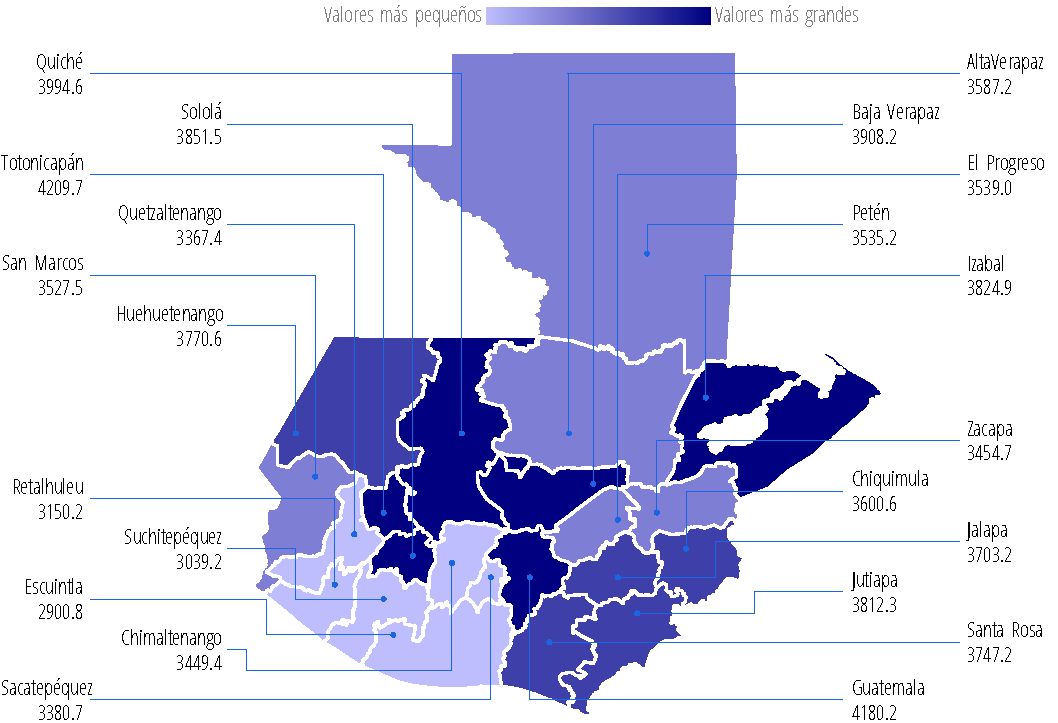
\includegraphics[width=52\cuadri]{graficas/3_06.pdf}}%
  {%
  	Instituto Guatemalteco de Seguridad Social} %

%#########################8########################

\cajita{%
	Costo de la canasta básica}%
{%
En cuanto al acceso de alimentos, en los indicadores sobre el precio de los alimentos, se muestra el costo diario promedio de la canasta básica alimentaria, este fue para el 2015 de Q 113.4.}%
{%
Costo  diario promedio de la canasta básica } %
{%
	República de Guatemala, serie histórica, en quetzales } %
{%
	\begin{tikzpicture}[x=1pt,y=1pt]  % Created by tikzDevice version 0.9 on 2016-03-03 04:35:21
% !TEX encoding = UTF-8 Unicode
\definecolor{fillColor}{RGB}{255,255,255}
\path[use as bounding box,fill=fillColor,fill opacity=0.00] (0,0) rectangle (289.08,198.74);
\begin{scope}
\path[clip] (  0.00,  0.00) rectangle (289.08,198.74);

\path[] (  0.00,  0.00) rectangle (289.08,198.74);
\end{scope}
\begin{scope}
\path[clip] (  0.00,  0.00) rectangle (289.08,198.74);

\path[] (  3.86, 15.61) rectangle (280.54,191.48);

\path[] (  3.86, 18.78) --
	(280.54, 18.78);

\path[] (  3.86, 52.84) --
	(280.54, 52.84);

\path[] (  3.86, 86.90) --
	(280.54, 86.90);

\path[] (  3.86,120.96) --
	(280.54,120.96);

\path[] (  3.86,155.02) --
	(280.54,155.02);

\path[] (  3.86,189.08) --
	(280.54,189.08);

\path[] (  3.86, 35.81) --
	(280.54, 35.81);

\path[] (  3.86, 69.87) --
	(280.54, 69.87);

\path[] (  3.86,103.93) --
	(280.54,103.93);

\path[] (  3.86,137.99) --
	(280.54,137.99);

\path[] (  3.86,172.05) --
	(280.54,172.05);

\path[] ( 35.79, 15.61) --
	( 35.79,191.48);

\path[] ( 88.99, 15.61) --
	( 88.99,191.48);

\path[] (142.20, 15.61) --
	(142.20,191.48);

\path[] (195.41, 15.61) --
	(195.41,191.48);

\path[] (248.62, 15.61) --
	(248.62,191.48);
\definecolor{drawColor}{RGB}{0,0,255}

\path[draw=drawColor,line width= 1.7pt,line join=round] ( 35.79, 60.50) --
	( 88.99, 86.42) --
	(142.20,114.46) --
	(195.41,144.18) --
	(248.62,183.49);
\definecolor{drawColor}{RGB}{0,0,0}

\node[text=drawColor,anchor=base,inner sep=0pt, outer sep=0pt, scale=  1.02] at ( 35.79, 48.59) {77.2};

\node[text=drawColor,anchor=base east,inner sep=0pt, outer sep=0pt, scale=  1.02] at ( 85.87, 86.42) {84.9};

\node[text=drawColor,anchor=base east,inner sep=0pt, outer sep=0pt, scale=  1.02] at (139.07,114.46) {93.1};

\node[text=drawColor,anchor=base east,inner sep=0pt, outer sep=0pt, scale=  1.02] at (191.39,144.18) {101.8};

\node[text=drawColor,anchor=base,inner sep=0pt, outer sep=0pt, scale=  1.02] at (248.62,187.46) {113.4};

\path[draw=drawColor,line width= 0.1pt,line join=round] (  3.86, 23.61) -- (280.54, 23.61);

\path[] (  3.86, 15.61) rectangle (280.54,191.48);
\end{scope}
\begin{scope}
\path[clip] (  0.00,  0.00) rectangle (289.08,198.74);

\path[] (  3.86, 15.61) --
	(  3.86,191.48);
\end{scope}
\begin{scope}
\path[clip] (  0.00,  0.00) rectangle (289.08,198.74);

\path[] (  1.11, 35.81) --
	(  3.86, 35.81);

\path[] (  1.11, 69.87) --
	(  3.86, 69.87);

\path[] (  1.11,103.93) --
	(  3.86,103.93);

\path[] (  1.11,137.99) --
	(  3.86,137.99);

\path[] (  1.11,172.05) --
	(  3.86,172.05);
\end{scope}
\begin{scope}
\path[clip] (  0.00,  0.00) rectangle (289.08,198.74);

\path[] (  3.86, 15.61) --
	(280.54, 15.61);
\end{scope}
\begin{scope}
\path[clip] (  0.00,  0.00) rectangle (289.08,198.74);

\path[] ( 35.79, 12.86) --
	( 35.79, 15.61);

\path[] ( 88.99, 12.86) --
	( 88.99, 15.61);

\path[] (142.20, 12.86) --
	(142.20, 15.61);

\path[] (195.41, 12.86) --
	(195.41, 15.61);

\path[] (248.62, 12.86) --
	(248.62, 15.61);
\end{scope}
\begin{scope}
\path[clip] (  0.00,  0.00) rectangle (289.08,198.74);
\definecolor{drawColor}{RGB}{0,0,0}

\node[text=drawColor,anchor=base,inner sep=0pt, outer sep=0pt, scale=  1.00] at ( 35.79,  2.85) {2011};

\node[text=drawColor,anchor=base,inner sep=0pt, outer sep=0pt, scale=  1.00] at ( 88.99,  2.85) {2012};

\node[text=drawColor,anchor=base,inner sep=0pt, outer sep=0pt, scale=  1.00] at (142.20,  2.85) {2013};

\node[text=drawColor,anchor=base,inner sep=0pt, outer sep=0pt, scale=  1.00] at (195.41,  2.85) {2014};

\node[text=drawColor,anchor=base,inner sep=0pt, outer sep=0pt, scale=  1.00] at (248.62,  2.85) {2015};
\end{scope}
  \end{tikzpicture}}%
{%
	Instituto Nacional de Estadística} %

%#########################9########################

\cajita{%
	Costo de la canasta básica ampliada}%
{%
En cuanto al costo promedio de la canasta básica vital o ampliada, en el 2015 este fue de Q 206.9.

La canasta básica vital incluye gastos de alimentación, vestuario y vivienda.}%
{%
	Costo diario promedio  de la canasta básica ampliada } %
{%
	República de Guatemala, serie histórica, en quetzales } %
{%
	\begin{tikzpicture}[x=1pt,y=1pt]  % Created by tikzDevice version 0.9 on 2016-03-03 04:35:29
% !TEX encoding = UTF-8 Unicode
\definecolor{fillColor}{RGB}{255,255,255}
\path[use as bounding box,fill=fillColor,fill opacity=0.00] (0,0) rectangle (289.08,198.74);
\begin{scope}
\path[clip] (  0.00,  0.00) rectangle (289.08,198.74);

\path[] (  0.00,  0.00) rectangle (289.08,198.74);
\end{scope}
\begin{scope}
\path[clip] (  0.00,  0.00) rectangle (289.08,198.74);

\path[] (  3.86, 15.61) rectangle (280.54,191.48);

\path[] (  3.86, 39.89) --
	(280.54, 39.89);

\path[] (  3.86, 77.26) --
	(280.54, 77.26);

\path[] (  3.86,114.62) --
	(280.54,114.62);

\path[] (  3.86,151.99) --
	(280.54,151.99);

\path[] (  3.86,189.36) --
	(280.54,189.36);

\path[] (  3.86, 21.20) --
	(280.54, 21.20);

\path[] (  3.86, 58.57) --
	(280.54, 58.57);

\path[] (  3.86, 95.94) --
	(280.54, 95.94);

\path[] (  3.86,133.31) --
	(280.54,133.31);

\path[] (  3.86,170.67) --
	(280.54,170.67);

\path[] ( 35.79, 15.61) --
	( 35.79,191.48);

\path[] ( 88.99, 15.61) --
	( 88.99,191.48);

\path[] (142.20, 15.61) --
	(142.20,191.48);

\path[] (195.41, 15.61) --
	(195.41,191.48);

\path[] (248.62, 15.61) --
	(248.62,191.48);
\definecolor{drawColor}{RGB}{0,0,255}

\path[draw=drawColor,line width= 1.7pt,line join=round] ( 35.79, 60.50) --
	( 88.99, 86.30) --
	(142.20,114.41) --
	(195.41,144.13) --
	(248.62,183.49);
\definecolor{drawColor}{RGB}{0,0,0}

\node[text=drawColor,anchor=base,inner sep=0pt, outer sep=0pt, scale=  1.02] at ( 35.79, 48.59) {141.0};

\node[text=drawColor,anchor=base east,inner sep=0pt, outer sep=0pt, scale=  1.02] at ( 84.98, 86.30) {154.8};

\node[text=drawColor,anchor=base east,inner sep=0pt, outer sep=0pt, scale=  1.02] at (138.18,114.41) {169.9};

\node[text=drawColor,anchor=base east,inner sep=0pt, outer sep=0pt, scale=  1.02] at (191.39,144.13) {185.8};

\node[text=drawColor,anchor=base,inner sep=0pt, outer sep=0pt, scale=  1.02] at (248.62,187.46) {206.9};

\path[draw=drawColor,line width= 0.1pt,line join=round] (  3.86, 23.61) -- (280.54, 23.61);

\path[] (  3.86, 15.61) rectangle (280.54,191.48);
\end{scope}
\begin{scope}
\path[clip] (  0.00,  0.00) rectangle (289.08,198.74);

\path[] (  3.86, 15.61) --
	(  3.86,191.48);
\end{scope}
\begin{scope}
\path[clip] (  0.00,  0.00) rectangle (289.08,198.74);

\path[] (  1.11, 21.20) --
	(  3.86, 21.20);

\path[] (  1.11, 58.57) --
	(  3.86, 58.57);

\path[] (  1.11, 95.94) --
	(  3.86, 95.94);

\path[] (  1.11,133.31) --
	(  3.86,133.31);

\path[] (  1.11,170.67) --
	(  3.86,170.67);
\end{scope}
\begin{scope}
\path[clip] (  0.00,  0.00) rectangle (289.08,198.74);

\path[] (  3.86, 15.61) --
	(280.54, 15.61);
\end{scope}
\begin{scope}
\path[clip] (  0.00,  0.00) rectangle (289.08,198.74);

\path[] ( 35.79, 12.86) --
	( 35.79, 15.61);

\path[] ( 88.99, 12.86) --
	( 88.99, 15.61);

\path[] (142.20, 12.86) --
	(142.20, 15.61);

\path[] (195.41, 12.86) --
	(195.41, 15.61);

\path[] (248.62, 12.86) --
	(248.62, 15.61);
\end{scope}
\begin{scope}
\path[clip] (  0.00,  0.00) rectangle (289.08,198.74);
\definecolor{drawColor}{RGB}{0,0,0}

\node[text=drawColor,anchor=base,inner sep=0pt, outer sep=0pt, scale=  1.00] at ( 35.79,  2.85) {2011};

\node[text=drawColor,anchor=base,inner sep=0pt, outer sep=0pt, scale=  1.00] at ( 88.99,  2.85) {2012};

\node[text=drawColor,anchor=base,inner sep=0pt, outer sep=0pt, scale=  1.00] at (142.20,  2.85) {2013};

\node[text=drawColor,anchor=base,inner sep=0pt, outer sep=0pt, scale=  1.00] at (195.41,  2.85) {2014};

\node[text=drawColor,anchor=base,inner sep=0pt, outer sep=0pt, scale=  1.00] at (248.62,  2.85) {2015};
\end{scope}
  \end{tikzpicture}}%
{%
	Instituto Nacional de Estadística} %

	\INEchaptercarta{Consumo de alimentos}{}
	%#########################1########################

 \cajita{%
Lactancia en niños menores de 5 años }%
{%
 }%
{%
 Niños menores de cinco años que lactaron alguna vez} %
{%
 República de Guatemala, 2008/2009, en porcentaje} %
{%
<<<<<<< HEAD
\small
%\ra{1.2}$\ $\\
\begin{tabular}{p{3.5cm}c}\hline
	\rowcolor{color2!0!white}&\\[-4mm]
	{\Bold   Característica}  & \textbf{Alguna vez recibió lactancia}\\
	\hline
	\rowcolor{color1!40!white} &\\[-4mm]
\rowcolor{color1!40!white}\textbf{Área geográfica}	&		\\
\rowcolor{color1!10!white}Urbana	&	94.4	\\
Rural	&	97.1	\\
\rowcolor{color1!40!white}\textbf{Región}	&		\\
\rowcolor{color1!0!white}Metropolitana	&	94.2	\\
Norte	&	95.9	\\
Nororiente	&	95.4	\\
Suroriente	&	93.7	\\
Central	&	96.5	\\
Suroccidente	&	97.1	\\
Noroccidente	&	97.3	\\
Petén	&	97.6	\\
\rowcolor{color1!40!white}\textbf{Categoría étnica de la madre}	&		\\
\rowcolor{color1!10!white}Indígena	&	97.1	\\
Ladino	&	95.2	\\
	\hline
	
\rowcolor{color1!0!white}	&\\[0.05cm]
\end{tabular}
}%
=======
}%
>>>>>>> origin/master
{%
 ENSMI 2008/2009} %


%#########################2########################

\cajita{%
	Duración de la lactancia según área de residencia}%
{%
}%
{%
	Duración de cualquier tipo de lactancia en niños menores de 2 años según área de residencia de la madre} %
{%
	República de Guatemala, 2008/2009, en meses} %
{%
	\begin{tikzpicture}[x=1pt,y=1pt]  % Created by tikzDevice version 0.9 on 2016-03-03 05:03:26
% !TEX encoding = UTF-8 Unicode
\definecolor{fillColor}{RGB}{255,255,255}
\path[use as bounding box,fill=fillColor,fill opacity=0.00] (0,0) rectangle (289.08,198.74);
\begin{scope}
\path[clip] (  0.00,  0.00) rectangle (289.08,198.74);

\path[] (  0.00,  0.00) rectangle (289.08,198.74);
\end{scope}
\begin{scope}
\path[clip] (  0.00,  0.00) rectangle (289.08,198.74);

\path[] (  0.00, 12.77) rectangle (289.08,181.67);

\path[] ( 78.84, 12.77) --
	( 78.84,181.67);

\path[] (210.24, 12.77) --
	(210.24,181.67);
\definecolor{drawColor}{RGB}{0,0,255}
\definecolor{fillColor}{RGB}{0,0,255}

\path[draw=drawColor,line width= 0.6pt,line join=round,fill=fillColor] ( 59.13, 20.44) rectangle ( 98.55,158.50);

\path[draw=drawColor,line width= 0.6pt,line join=round,fill=fillColor] (190.53, 20.44) rectangle (229.95,173.99);
\definecolor{drawColor}{RGB}{0,0,0}

\path[draw=drawColor,line width= 0.1pt,line join=round] (  0.00, 20.44) -- (289.08, 20.44);

\node[text=drawColor,anchor=base,inner sep=0pt, outer sep=0pt, scale=  1.02] at ( 78.84,162.47) {19.6};

\node[text=drawColor,anchor=base,inner sep=0pt, outer sep=0pt, scale=  1.02] at (210.24,177.96) {21.8};

\path[] (  0.00, 12.77) rectangle (289.08,181.67);
\end{scope}
\begin{scope}
\path[clip] (  0.00,  0.00) rectangle (289.08,198.74);

\path[] (  0.00, 12.77) --
	(289.08, 12.77);
\end{scope}
\begin{scope}
\path[clip] (  0.00,  0.00) rectangle (289.08,198.74);

\path[] ( 78.84, 10.02) --
	( 78.84, 12.77);

\path[] (210.24, 10.02) --
	(210.24, 12.77);
\end{scope}
\begin{scope}
\path[clip] (  0.00,  0.00) rectangle (289.08,198.74);
\definecolor{drawColor}{RGB}{0,0,0}

\node[text=drawColor,anchor=base,inner sep=0pt, outer sep=0pt, scale=  1.00] at ( 78.84, -0.00) {Urbana};

\node[text=drawColor,anchor=base,inner sep=0pt, outer sep=0pt, scale=  1.00] at (210.24, -0.00) {Rural};
\end{scope}
  \end{tikzpicture}
}%
{%
	ENSMI 2008/2009} %


%#########################3########################

\cajita{%
	Duración de la lactancia según etnia}%
{%
}%
{%
	Duración de cualquier tipo de lactancia en niños menores de 2 años según etnia de la madre} %
{%
	República de Guatemala, 2008/2009, en meses} %
{%
	\begin{tikzpicture}[x=1pt,y=1pt]  % Created by tikzDevice version 0.9 on 2016-03-03 05:04:33
% !TEX encoding = UTF-8 Unicode
\definecolor{fillColor}{RGB}{255,255,255}
\path[use as bounding box,fill=fillColor,fill opacity=0.00] (0,0) rectangle (289.08,198.74);
\begin{scope}
\path[clip] (  0.00,  0.00) rectangle (289.08,198.74);

\path[] (  0.00,  0.00) rectangle (289.08,198.74);
\end{scope}
\begin{scope}
\path[clip] (  0.00,  0.00) rectangle (289.08,198.74);

\path[] (  0.00, 12.77) rectangle (289.08,181.67);

\path[] ( 78.84, 12.77) --
	( 78.84,181.67);

\path[] (210.24, 12.77) --
	(210.24,181.67);
\definecolor{drawColor}{RGB}{0,0,255}
\definecolor{fillColor}{RGB}{0,0,255}

\path[draw=drawColor,line width= 0.6pt,line join=round,fill=fillColor] ( 59.13, 20.44) rectangle ( 98.55,173.99);

\path[draw=drawColor,line width= 0.6pt,line join=round,fill=fillColor] (190.53, 20.44) rectangle (229.95,142.06);
\definecolor{drawColor}{RGB}{0,0,0}

\path[draw=drawColor,line width= 0.1pt,line join=round] (  0.00, 20.44) -- (289.08, 20.44);

\node[text=drawColor,anchor=base,inner sep=0pt, outer sep=0pt, scale=  1.02] at ( 78.84,177.96) {22.6};

\node[text=drawColor,anchor=base,inner sep=0pt, outer sep=0pt, scale=  1.02] at (210.24,146.03) {17.9};

\path[] (  0.00, 12.77) rectangle (289.08,181.67);
\end{scope}
\begin{scope}
\path[clip] (  0.00,  0.00) rectangle (289.08,198.74);

\path[] (  0.00, 12.77) --
	(289.08, 12.77);
\end{scope}
\begin{scope}
\path[clip] (  0.00,  0.00) rectangle (289.08,198.74);

\path[] ( 78.84, 10.02) --
	( 78.84, 12.77);

\path[] (210.24, 10.02) --
	(210.24, 12.77);
\end{scope}
\begin{scope}
\path[clip] (  0.00,  0.00) rectangle (289.08,198.74);
\definecolor{drawColor}{RGB}{0,0,0}

\node[text=drawColor,anchor=base,inner sep=0pt, outer sep=0pt, scale=  1.00] at ( 78.84, -0.00) {Indígena};

\node[text=drawColor,anchor=base,inner sep=0pt, outer sep=0pt, scale=  1.00] at (210.24, -0.00) {Ladino};
\end{scope}
  \end{tikzpicture}
}%
{%
	ENSMI 2008/2009} %

%#########################4########################

\cajita{%
	Duración de la lactancia por educación}%
{%
}%
{%
	Duración de cualquier tipo de lactancia en niños menores de 2 años según el grado de educación de la madre} %
{%
	República de Guatemala, 2008/2009, en meses} %
{%
	\begin{tikzpicture}[x=1pt,y=1pt]  % Created by tikzDevice version 0.9 on 2016-03-03 04:58:10
% !TEX encoding = UTF-8 Unicode
\definecolor{fillColor}{RGB}{255,255,255}
\path[use as bounding box,fill=fillColor,fill opacity=0.00] (0,0) rectangle (289.08,198.74);
\begin{scope}
\path[clip] (  0.00,  0.00) rectangle (289.08,198.74);

\path[] (  0.00,  0.00) rectangle (289.08,198.74);
\end{scope}
\begin{scope}
\path[clip] (  0.00,  0.00) rectangle (289.08,198.74);

\path[] (  0.00, 12.77) rectangle (289.08,181.67);

\path[] ( 41.30, 12.77) --
	( 41.30,181.67);

\path[] (110.13, 12.77) --
	(110.13,181.67);

\path[] (178.95, 12.77) --
	(178.95,181.67);

\path[] (247.78, 12.77) --
	(247.78,181.67);
\definecolor{drawColor}{RGB}{0,0,255}
\definecolor{fillColor}{RGB}{0,0,255}

\path[draw=drawColor,line width= 0.6pt,line join=round,fill=fillColor] ( 24.09, 20.44) rectangle ( 58.50,173.99);

\path[draw=drawColor,line width= 0.6pt,line join=round,fill=fillColor] ( 92.92, 20.44) rectangle (127.33,169.79);

\path[draw=drawColor,line width= 0.6pt,line join=round,fill=fillColor] (161.75, 20.44) rectangle (196.16,119.30);

\path[draw=drawColor,line width= 0.6pt,line join=round,fill=fillColor] (230.58, 20.44) rectangle (264.99, 77.24);
\definecolor{drawColor}{RGB}{0,0,0}

\path[draw=drawColor,line width= 0.1pt,line join=round] (  0.00, 20.44) -- (289.08, 20.44);

\node[text=drawColor,anchor=base,inner sep=0pt, outer sep=0pt, scale=  1.02] at ( 41.30,177.96) {21.9};

\node[text=drawColor,anchor=base,inner sep=0pt, outer sep=0pt, scale=  1.02] at (110.13,173.76) {21.3};

\node[text=drawColor,anchor=base,inner sep=0pt, outer sep=0pt, scale=  1.02] at (178.95,123.28) {14.1};

\node[text=drawColor,anchor=base,inner sep=0pt, outer sep=0pt, scale=  1.02] at (247.78, 81.21) {8.1};

\path[] (  0.00, 12.77) rectangle (289.08,181.67);
\end{scope}
\begin{scope}
\path[clip] (  0.00,  0.00) rectangle (289.08,198.74);

\path[] (  0.00, 12.77) --
	(289.08, 12.77);
\end{scope}
\begin{scope}
\path[clip] (  0.00,  0.00) rectangle (289.08,198.74);

\path[] ( 41.30, 10.02) --
	( 41.30, 12.77);

\path[] (110.13, 10.02) --
	(110.13, 12.77);

\path[] (178.95, 10.02) --
	(178.95, 12.77);

\path[] (247.78, 10.02) --
	(247.78, 12.77);
\end{scope}
\begin{scope}
\path[clip] (  0.00,  0.00) rectangle (289.08,198.74);
\definecolor{drawColor}{RGB}{0,0,0}

\node[text=drawColor,anchor=base,inner sep=0pt, outer sep=0pt, scale=  1.00] at ( 41.30, -0.00) {Ninguna};

\node[text=drawColor,anchor=base,inner sep=0pt, outer sep=0pt, scale=  1.00] at (110.13, -0.00) {Primaria};

\node[text=drawColor,anchor=base,inner sep=0pt, outer sep=0pt, scale=  1.00] at (178.95, -0.00) {Secundaria};

\node[text=drawColor,anchor=base,inner sep=0pt, outer sep=0pt, scale=  1.00] at (247.78, -0.00) {Superior};
\end{scope}
  \end{tikzpicture}
}%
{%
	ENSMI 2008/2009} %


%#########################5########################

\cajita{%
Niños de 0 a 3 meses según lactancia}%
{%
}%
{%
	Distribución de niños de 0 a 3 meses según lactancia y área de residencia
	} %
{%
	República de Guatemala, 2008/2009, en meses} %
{%
	\begin{tikzpicture}[x=1pt,y=1pt]  % Created by tikzDevice version 0.9 on 2016-03-03 04:58:13
% !TEX encoding = UTF-8 Unicode
\definecolor{fillColor}{RGB}{255,255,255}
\path[use as bounding box,fill=fillColor,fill opacity=0.00] (0,0) rectangle (289.08,198.74);
\begin{scope}
\path[clip] (  0.00,  0.00) rectangle (289.08,198.74);

\path[] (  0.00,  0.00) rectangle (289.08,198.74);
\end{scope}
\begin{scope}
\path[clip] (  0.00,  0.00) rectangle (289.08,198.74);

\path[] (  0.00, 18.46) rectangle (289.08,166.57);

\path[] ( 54.20, 18.46) --
	( 54.20,166.57);

\path[] (144.54, 18.46) --
	(144.54,166.57);

\path[] (234.88, 18.46) --
	(234.88,166.57);
\definecolor{drawColor}{RGB}{0,0,255}
\definecolor{fillColor}{RGB}{0,0,255}

\path[draw=drawColor,line width= 0.6pt,line join=round,fill=fillColor] ( 15.81, 18.46) rectangle ( 51.94, 30.54);
\definecolor{drawColor}{RGB}{157,187,255}
\definecolor{fillColor}{RGB}{157,187,255}

\path[draw=drawColor,line width= 0.6pt,line join=round,fill=fillColor] ( 56.46, 18.46) rectangle ( 92.60, 25.71);
\definecolor{drawColor}{RGB}{0,0,255}
\definecolor{fillColor}{RGB}{0,0,255}

\path[draw=drawColor,line width= 0.6pt,line join=round,fill=fillColor] (106.15, 18.46) rectangle (142.28,101.75);
\definecolor{drawColor}{RGB}{157,187,255}
\definecolor{fillColor}{RGB}{157,187,255}

\path[draw=drawColor,line width= 0.6pt,line join=round,fill=fillColor] (146.80, 18.46) rectangle (182.93,166.57);
\definecolor{drawColor}{RGB}{0,0,255}
\definecolor{fillColor}{RGB}{0,0,255}

\path[draw=drawColor,line width= 0.6pt,line join=round,fill=fillColor] (196.48, 18.46) rectangle (232.62, 72.08);
\definecolor{drawColor}{RGB}{157,187,255}
\definecolor{fillColor}{RGB}{157,187,255}

\path[draw=drawColor,line width= 0.6pt,line join=round,fill=fillColor] (237.14, 18.46) rectangle (273.27, 59.33);
\definecolor{drawColor}{RGB}{0,0,0}

\path[draw=drawColor,line width= 0.6pt,line join=round] (  0.00, 18.46) -- (289.08, 18.46);

\node[text=drawColor,rotate= 90.00,anchor=base west,inner sep=0pt, outer sep=0pt, scale=  0.83] at ( 37.11, 32.37) {5.5};

\node[text=drawColor,rotate= 90.00,anchor=base west,inner sep=0pt, outer sep=0pt, scale=  0.83] at ( 77.76, 27.53) {3.3};

\node[text=drawColor,rotate= 90.00,anchor=base west,inner sep=0pt, outer sep=0pt, scale=  0.83] at (127.45,104.29) {37.9};

\node[text=drawColor,rotate= 90.00,anchor=base west,inner sep=0pt, outer sep=0pt, scale=  0.83] at (168.10,169.12) {67.4};

\node[text=drawColor,rotate= 90.00,anchor=base west,inner sep=0pt, outer sep=0pt, scale=  0.83] at (217.79, 74.63) {24.4};

\node[text=drawColor,rotate= 90.00,anchor=base west,inner sep=0pt, outer sep=0pt, scale=  0.83] at (258.44, 61.88) {18.6};

\path[] (  0.00, 18.46) rectangle (289.08,166.57);
\end{scope}
\begin{scope}
\path[clip] (  0.00,  0.00) rectangle (289.08,198.74);

\path[] (  0.00, 18.46) --
	(289.08, 18.46);
\end{scope}
\begin{scope}
\path[clip] (  0.00,  0.00) rectangle (289.08,198.74);

\path[] ( 54.20, 15.71) --
	( 54.20, 18.46);

\path[] (144.54, 15.71) --
	(144.54, 18.46);

\path[] (234.88, 15.71) --
	(234.88, 18.46);
\end{scope}
\begin{scope}
\path[clip] (  0.00,  0.00) rectangle (289.08,198.74);
\definecolor{drawColor}{RGB}{0,0,0}

\node[text=drawColor,anchor=base,inner sep=0pt, outer sep=0pt, scale=  1.00] at ( 54.20,  5.69) {No lactando};

\node[text=drawColor,anchor=base,inner sep=0pt, outer sep=0pt, scale=  1.00] at (144.54,  5.69) {Lactancia Exclusiva};

\node[text=drawColor,anchor=base,inner sep=0pt, outer sep=0pt, scale=  1.00] at (234.88,  5.69) {Lactancia Predominante};
\end{scope}
\begin{scope}
\path[clip] (  0.00,  0.00) rectangle (289.08,198.74);
\coordinate (apoyo) at (57.27,191.13);
\coordinate (longitudFicticia) at (7.11,7.61);
\coordinate (longitud) at (7.11,7.11);
\coordinate (desX) at (142.24,0);
\coordinate (desY) at (0,0.25);
\definecolor[named]{ct1}{HTML}{
0000FF
}
\definecolor[named]{ct2}{HTML}{
9DBBFF
}
\definecolor[named]{ctb1}{HTML}{
0000FF
}
\definecolor[named]{ctb2}{HTML}{
9DBBFF
}
\path [fill=none] (apoyo) rectangle ($(apoyo)+(longitudFicticia)$)
node [xshift=0.3cm,inner sep=0pt, outer sep=0pt,midway,right,scale = 0.9]{Urbana};
\draw [color = ctb1,fill=ct1] ( $(apoyo)  + (desY) $) rectangle ($(apoyo)+ (desY) +(longitud)$);
\path [fill=none] ($(apoyo)+(desX)$) rectangle ($(apoyo)+(desX)+(longitudFicticia)$)
node [xshift=0.3cm,inner sep=0pt, outer sep=0pt,midway,right,scale = 0.9]{Rural};
\draw [color = ctb2 ,fill=ct2] ( $(apoyo)  + (desY) + (desX) $) rectangle ($(apoyo)+ (desY)+ (desX) +(longitud)$);
\end{scope}
  \end{tikzpicture}
}%
{%
	ENSMI 2008/2009} %


%#########################6########################

\cajita{%
	Niños de 0 a 3 meses según lactancia por etnia}%
{%
}%
{%
	Distribución de niños de 0 a 3 meses según lactancia y etnia
} %
{%
	República de Guatemala, 2008/2009, en meses} %
{%
	\begin{tikzpicture}[x=1pt,y=1pt]  % Created by tikzDevice version 0.9 on 2016-03-03 04:58:20
% !TEX encoding = UTF-8 Unicode
\definecolor{fillColor}{RGB}{255,255,255}
\path[use as bounding box,fill=fillColor,fill opacity=0.00] (0,0) rectangle (289.08,198.74);
\begin{scope}
\path[clip] (  0.00,  0.00) rectangle (289.08,198.74);

\path[] (  0.00,  0.00) rectangle (289.08,198.74);
\end{scope}
\begin{scope}
\path[clip] (  0.00,  0.00) rectangle (289.08,198.74);

\path[] (  0.00, 18.46) rectangle (289.08,164.23);

\path[] ( 54.20, 18.46) --
	( 54.20,164.23);

\path[] (144.54, 18.46) --
	(144.54,164.23);

\path[] (234.88, 18.46) --
	(234.88,164.23);
\definecolor{drawColor}{RGB}{0,0,255}
\definecolor{fillColor}{RGB}{0,0,255}

\path[draw=drawColor,line width= 0.6pt,line join=round,fill=fillColor] ( 15.81, 18.46) rectangle ( 51.94, 26.18);
\definecolor{drawColor}{RGB}{157,187,255}
\definecolor{fillColor}{RGB}{157,187,255}

\path[draw=drawColor,line width= 0.6pt,line join=round,fill=fillColor] ( 56.46, 18.46) rectangle ( 92.60, 27.61);
\definecolor{drawColor}{RGB}{0,0,255}
\definecolor{fillColor}{RGB}{0,0,255}

\path[draw=drawColor,line width= 0.6pt,line join=round,fill=fillColor] (106.15, 18.46) rectangle (142.28,164.23);
\definecolor{drawColor}{RGB}{157,187,255}
\definecolor{fillColor}{RGB}{157,187,255}

\path[draw=drawColor,line width= 0.6pt,line join=round,fill=fillColor] (146.80, 18.46) rectangle (182.93,102.43);
\definecolor{drawColor}{RGB}{0,0,255}
\definecolor{fillColor}{RGB}{0,0,255}

\path[draw=drawColor,line width= 0.6pt,line join=round,fill=fillColor] (196.48, 18.46) rectangle (232.62, 47.73);
\definecolor{drawColor}{RGB}{157,187,255}
\definecolor{fillColor}{RGB}{157,187,255}

\path[draw=drawColor,line width= 0.6pt,line join=round,fill=fillColor] (237.14, 18.46) rectangle (273.27, 72.74);
\definecolor{drawColor}{RGB}{0,0,0}

\path[draw=drawColor,line width= 0.6pt,line join=round] (  0.00, 18.46) -- (289.08, 18.46);

\node[text=drawColor,rotate= 90.00,anchor=base west,inner sep=0pt, outer sep=0pt, scale=  0.83] at ( 37.11, 28.01) {3.8};

\node[text=drawColor,rotate= 90.00,anchor=base west,inner sep=0pt, outer sep=0pt, scale=  0.83] at ( 77.76, 29.43) {4.5};

\node[text=drawColor,rotate= 90.00,anchor=base west,inner sep=0pt, outer sep=0pt, scale=  0.83] at (127.45,166.78) {71.7};

\node[text=drawColor,rotate= 90.00,anchor=base west,inner sep=0pt, outer sep=0pt, scale=  0.83] at (168.10,104.97) {41.3};

\node[text=drawColor,rotate= 90.00,anchor=base west,inner sep=0pt, outer sep=0pt, scale=  0.83] at (217.79, 50.28) {14.4};

\node[text=drawColor,rotate= 90.00,anchor=base west,inner sep=0pt, outer sep=0pt, scale=  0.83] at (258.44, 75.29) {26.7};

\path[] (  0.00, 18.46) rectangle (289.08,164.23);
\end{scope}
\begin{scope}
\path[clip] (  0.00,  0.00) rectangle (289.08,198.74);

\path[] (  0.00, 18.46) --
	(289.08, 18.46);
\end{scope}
\begin{scope}
\path[clip] (  0.00,  0.00) rectangle (289.08,198.74);

\path[] ( 54.20, 15.71) --
	( 54.20, 18.46);

\path[] (144.54, 15.71) --
	(144.54, 18.46);

\path[] (234.88, 15.71) --
	(234.88, 18.46);
\end{scope}
\begin{scope}
\path[clip] (  0.00,  0.00) rectangle (289.08,198.74);
\definecolor{drawColor}{RGB}{0,0,0}

\node[text=drawColor,anchor=base,inner sep=0pt, outer sep=0pt, scale=  1.00] at ( 54.20,  5.69) {No lactando};

\node[text=drawColor,anchor=base,inner sep=0pt, outer sep=0pt, scale=  1.00] at (144.54,  5.69) {Lactancia Exclusiva};

\node[text=drawColor,anchor=base,inner sep=0pt, outer sep=0pt, scale=  1.00] at (234.88,  5.69) {Lactancia Predominante};
\end{scope}
\begin{scope}
\path[clip] (  0.00,  0.00) rectangle (289.08,198.74);
\coordinate (apoyo) at (55.19,188.79);
\coordinate (longitudFicticia) at (7.11,9.95);
\coordinate (longitud) at (7.11,7.11);
\coordinate (desX) at (133.24,0);
\coordinate (desY) at (0,1.42);
\definecolor[named]{ct1}{HTML}{
0000FF
}
\definecolor[named]{ct2}{HTML}{
9DBBFF
}
\definecolor[named]{ctb1}{HTML}{
0000FF
}
\definecolor[named]{ctb2}{HTML}{
9DBBFF
}
\path [fill=none] (apoyo) rectangle ($(apoyo)+(longitudFicticia)$)
node [xshift=0.3cm,inner sep=0pt, outer sep=0pt,midway,right,scale = 0.9]{Indígena};
\draw [color = ctb1,fill=ct1] ( $(apoyo)  + (desY) $) rectangle ($(apoyo)+ (desY) +(longitud)$);
\path [fill=none] ($(apoyo)+(desX)$) rectangle ($(apoyo)+(desX)+(longitudFicticia)$)
node [xshift=0.3cm,inner sep=0pt, outer sep=0pt,midway,right,scale = 0.9]{No indígena};
\draw [color = ctb2 ,fill=ct2] ( $(apoyo)  + (desY) + (desX) $) rectangle ($(apoyo)+ (desY)+ (desX) +(longitud)$);
\end{scope}
  \end{tikzpicture}
}%
{%
	ENSMI 2008/2009} %


%#########################7########################

\cajita{%
	Niños de 0 a 3 meses según lactancia y educación de la madre}%
{%
}%
{%
	Distribución de niños de 0 a 3 meses según lactancia y educación de la madre
} %
{%
	República de Guatemala, 2008/2009, en meses} %
{%
	\begin{tikzpicture}[x=1pt,y=1pt]  % Created by tikzDevice version 0.9 on 2016-03-03 04:58:26
% !TEX encoding = UTF-8 Unicode
\definecolor{fillColor}{RGB}{255,255,255}
\path[use as bounding box,fill=fillColor,fill opacity=0.00] (0,0) rectangle (289.08,198.74);
\begin{scope}
\path[clip] (  0.00,  0.00) rectangle (289.08,198.74);

\path[] (  0.00,  0.00) rectangle (289.08,198.74);
\end{scope}
\begin{scope}
\path[clip] (  0.00,  0.00) rectangle (289.08,198.74);

\path[] (  0.00, 18.46) rectangle (289.08,164.65);

\path[] ( 54.20, 18.46) --
	( 54.20,164.65);

\path[] (144.54, 18.46) --
	(144.54,164.65);

\path[] (234.88, 18.46) --
	(234.88,164.65);
\definecolor{drawColor}{RGB}{0,0,255}
\definecolor{fillColor}{RGB}{0,0,255}

\path[draw=drawColor,line width= 0.6pt,line join=round,fill=fillColor] ( 15.81, 18.46) rectangle ( 51.94, 26.28);
\definecolor{drawColor}{RGB}{157,187,255}
\definecolor{fillColor}{RGB}{157,187,255}

\path[draw=drawColor,line width= 0.6pt,line join=round,fill=fillColor] ( 56.46, 18.46) rectangle ( 92.60, 26.93);
\definecolor{drawColor}{RGB}{0,0,255}
\definecolor{fillColor}{RGB}{0,0,255}

\path[draw=drawColor,line width= 0.6pt,line join=round,fill=fillColor] (106.15, 18.46) rectangle (142.28,164.65);
\definecolor{drawColor}{RGB}{157,187,255}
\definecolor{fillColor}{RGB}{157,187,255}

\path[draw=drawColor,line width= 0.6pt,line join=round,fill=fillColor] (146.80, 18.46) rectangle (182.93, 30.84);
\definecolor{drawColor}{RGB}{0,0,255}
\definecolor{fillColor}{RGB}{0,0,255}

\path[draw=drawColor,line width= 0.6pt,line join=round,fill=fillColor] (196.48, 18.46) rectangle (232.62, 67.33);
\definecolor{drawColor}{RGB}{157,187,255}
\definecolor{fillColor}{RGB}{157,187,255}

\path[draw=drawColor,line width= 0.6pt,line join=round,fill=fillColor] (237.14, 18.46) rectangle (273.27, 44.52);
\definecolor{drawColor}{RGB}{0,0,0}

\path[draw=drawColor,line width= 0.6pt,line join=round] (  0.00, 18.46) -- (289.08, 18.46);

\node[text=drawColor,rotate= 90.00,anchor=base west,inner sep=0pt, outer sep=0pt, scale=  0.83] at ( 37.11, 28.10) {3.6};

\node[text=drawColor,rotate= 90.00,anchor=base west,inner sep=0pt, outer sep=0pt, scale=  0.83] at ( 77.76, 28.75) {3.9};

\node[text=drawColor,rotate= 90.00,anchor=base west,inner sep=0pt, outer sep=0pt, scale=  0.83] at (127.45,167.20) {67.3};

\node[text=drawColor,rotate= 90.00,anchor=base west,inner sep=0pt, outer sep=0pt, scale=  0.83] at (168.10, 32.66) {5.7};

\node[text=drawColor,rotate= 90.00,anchor=base west,inner sep=0pt, outer sep=0pt, scale=  0.83] at (217.79, 69.88) {22.5};

\node[text=drawColor,rotate= 90.00,anchor=base west,inner sep=0pt, outer sep=0pt, scale=  0.83] at (258.44, 47.07) {12.0};

\path[] (  0.00, 18.46) rectangle (289.08,164.65);
\end{scope}
\begin{scope}
\path[clip] (  0.00,  0.00) rectangle (289.08,198.74);

\path[] (  0.00, 18.46) --
	(289.08, 18.46);
\end{scope}
\begin{scope}
\path[clip] (  0.00,  0.00) rectangle (289.08,198.74);

\path[] ( 54.20, 15.71) --
	( 54.20, 18.46);

\path[] (144.54, 15.71) --
	(144.54, 18.46);

\path[] (234.88, 15.71) --
	(234.88, 18.46);
\end{scope}
\begin{scope}
\path[clip] (  0.00,  0.00) rectangle (289.08,198.74);
\definecolor{drawColor}{RGB}{0,0,0}

\node[text=drawColor,anchor=base,inner sep=0pt, outer sep=0pt, scale=  1.00] at ( 54.20,  5.69) {No lactando};

\node[text=drawColor,anchor=base,inner sep=0pt, outer sep=0pt, scale=  1.00] at (144.54,  5.69) {Lactancia Exclusiva};

\node[text=drawColor,anchor=base,inner sep=0pt, outer sep=0pt, scale=  1.00] at (234.88,  5.69) {Lactancia Predominante};
\end{scope}
\begin{scope}
\path[clip] (  0.00,  0.00) rectangle (289.08,198.74);
\coordinate (apoyo) at (46.95,189.2);
\coordinate (longitudFicticia) at (7.11,9.54);
\coordinate (longitud) at (7.11,7.11);
\coordinate (desX) at (147.1,0);
\coordinate (desY) at (0,1.21);
\definecolor[named]{ct1}{HTML}{
0000FF
}
\definecolor[named]{ct2}{HTML}{
9DBBFF
}
\definecolor[named]{ctb1}{HTML}{
0000FF
}
\definecolor[named]{ctb2}{HTML}{
9DBBFF
}
\path [fill=none] (apoyo) rectangle ($(apoyo)+(longitudFicticia)$)
node [xshift=0.3cm,inner sep=0pt, outer sep=0pt,midway,right,scale = 0.9]{Sin educación};
\draw [color = ctb1,fill=ct1] ( $(apoyo)  + (desY) $) rectangle ($(apoyo)+ (desY) +(longitud)$);
\path [fill=none] ($(apoyo)+(desX)$) rectangle ($(apoyo)+(desX)+(longitudFicticia)$)
node [xshift=0.3cm,inner sep=0pt, outer sep=0pt,midway,right,scale = 0.9]{Superior};
\draw [color = ctb2 ,fill=ct2] ( $(apoyo)  + (desY) + (desX) $) rectangle ($(apoyo)+ (desY)+ (desX) +(longitud)$);
\end{scope}
  \end{tikzpicture}
}%
{%
	ENSMI 2008/2009} %

%#########################8########################

\cajita{%
	Niños de 0 a 5 meses según lactancia}%
{%
}%
{%
	Distribución de niños de 0 a 5 meses según lactancia y área de residencia
} %
{%
	República de Guatemala, 2008/2009, en meses} %
{%
	\begin{tikzpicture}[x=1pt,y=1pt]  % Created by tikzDevice version 0.9 on 2016-03-03 04:58:32
% !TEX encoding = UTF-8 Unicode
\definecolor{fillColor}{RGB}{255,255,255}
\path[use as bounding box,fill=fillColor,fill opacity=0.00] (0,0) rectangle (289.08,198.74);
\begin{scope}
\path[clip] (  0.00,  0.00) rectangle (289.08,198.74);

\path[] (  0.00,  0.00) rectangle (289.08,198.74);
\end{scope}
\begin{scope}
\path[clip] (  0.00,  0.00) rectangle (289.08,198.74);

\path[] (  0.00, 18.46) rectangle (289.08,166.57);

\path[] ( 54.20, 18.46) --
	( 54.20,166.57);

\path[] (144.54, 18.46) --
	(144.54,166.57);

\path[] (234.88, 18.46) --
	(234.88,166.57);
\definecolor{drawColor}{RGB}{0,0,255}
\definecolor{fillColor}{RGB}{0,0,255}

\path[draw=drawColor,line width= 0.6pt,line join=round,fill=fillColor] ( 15.81, 18.46) rectangle ( 51.94, 42.73);
\definecolor{drawColor}{RGB}{157,187,255}
\definecolor{fillColor}{RGB}{157,187,255}

\path[draw=drawColor,line width= 0.6pt,line join=round,fill=fillColor] ( 56.46, 18.46) rectangle ( 92.60, 26.80);
\definecolor{drawColor}{RGB}{0,0,255}
\definecolor{fillColor}{RGB}{0,0,255}

\path[draw=drawColor,line width= 0.6pt,line join=round,fill=fillColor] (106.15, 18.46) rectangle (142.28, 98.16);
\definecolor{drawColor}{RGB}{157,187,255}
\definecolor{fillColor}{RGB}{157,187,255}

\path[draw=drawColor,line width= 0.6pt,line join=round,fill=fillColor] (146.80, 18.46) rectangle (182.93,166.57);
\definecolor{drawColor}{RGB}{0,0,255}
\definecolor{fillColor}{RGB}{0,0,255}

\path[draw=drawColor,line width= 0.6pt,line join=round,fill=fillColor] (196.48, 18.46) rectangle (232.62, 73.88);
\definecolor{drawColor}{RGB}{157,187,255}
\definecolor{fillColor}{RGB}{157,187,255}

\path[draw=drawColor,line width= 0.6pt,line join=round,fill=fillColor] (237.14, 18.46) rectangle (273.27, 61.13);
\definecolor{drawColor}{RGB}{0,0,0}

\path[draw=drawColor,line width= 0.6pt,line join=round] (  0.00, 18.46) -- (289.08, 18.46);

\node[text=drawColor,rotate= 90.00,anchor=base west,inner sep=0pt, outer sep=0pt, scale=  0.83] at ( 37.11, 44.56) {9.9};

\node[text=drawColor,rotate= 90.00,anchor=base west,inner sep=0pt, outer sep=0pt, scale=  0.83] at ( 77.76, 28.62) {3.4};

\node[text=drawColor,rotate= 90.00,anchor=base west,inner sep=0pt, outer sep=0pt, scale=  0.83] at (127.45,100.70) {32.5};

\node[text=drawColor,rotate= 90.00,anchor=base west,inner sep=0pt, outer sep=0pt, scale=  0.83] at (168.10,169.12) {60.4};

\node[text=drawColor,rotate= 90.00,anchor=base west,inner sep=0pt, outer sep=0pt, scale=  0.83] at (217.79, 76.43) {22.6};

\node[text=drawColor,rotate= 90.00,anchor=base west,inner sep=0pt, outer sep=0pt, scale=  0.83] at (258.44, 63.68) {17.4};

\path[] (  0.00, 18.46) rectangle (289.08,166.57);
\end{scope}
\begin{scope}
\path[clip] (  0.00,  0.00) rectangle (289.08,198.74);

\path[] (  0.00, 18.46) --
	(289.08, 18.46);
\end{scope}
\begin{scope}
\path[clip] (  0.00,  0.00) rectangle (289.08,198.74);

\path[] ( 54.20, 15.71) --
	( 54.20, 18.46);

\path[] (144.54, 15.71) --
	(144.54, 18.46);

\path[] (234.88, 15.71) --
	(234.88, 18.46);
\end{scope}
\begin{scope}
\path[clip] (  0.00,  0.00) rectangle (289.08,198.74);
\definecolor{drawColor}{RGB}{0,0,0}

\node[text=drawColor,anchor=base,inner sep=0pt, outer sep=0pt, scale=  1.00] at ( 54.20,  5.69) {No lactando};

\node[text=drawColor,anchor=base,inner sep=0pt, outer sep=0pt, scale=  1.00] at (144.54,  5.69) {Lactancia Exclusiva};

\node[text=drawColor,anchor=base,inner sep=0pt, outer sep=0pt, scale=  1.00] at (234.88,  5.69) {Lactancia Predominante};
\end{scope}
\begin{scope}
\path[clip] (  0.00,  0.00) rectangle (289.08,198.74);
\coordinate (apoyo) at (57.27,191.13);
\coordinate (longitudFicticia) at (7.11,7.61);
\coordinate (longitud) at (7.11,7.11);
\coordinate (desX) at (142.24,0);
\coordinate (desY) at (0,0.25);
\definecolor[named]{ct1}{HTML}{
0000FF
}
\definecolor[named]{ct2}{HTML}{
9DBBFF
}
\definecolor[named]{ctb1}{HTML}{
0000FF
}
\definecolor[named]{ctb2}{HTML}{
9DBBFF
}
\path [fill=none] (apoyo) rectangle ($(apoyo)+(longitudFicticia)$)
node [xshift=0.3cm,inner sep=0pt, outer sep=0pt,midway,right,scale = 0.9]{Urbana};
\draw [color = ctb1,fill=ct1] ( $(apoyo)  + (desY) $) rectangle ($(apoyo)+ (desY) +(longitud)$);
\path [fill=none] ($(apoyo)+(desX)$) rectangle ($(apoyo)+(desX)+(longitudFicticia)$)
node [xshift=0.3cm,inner sep=0pt, outer sep=0pt,midway,right,scale = 0.9]{Rural};
\draw [color = ctb2 ,fill=ct2] ( $(apoyo)  + (desY) + (desX) $) rectangle ($(apoyo)+ (desY)+ (desX) +(longitud)$);
\end{scope}
  \end{tikzpicture}
}%
{%
	ENSMI 2008/2009} %


%#########################9########################

\cajita{%
	Niños de 0 a 5 meses según lactancia por etnia}%
{%
}%
{%
	Distribución de niños de 0 a 5 meses según lactancia y etnia
} %
{%
	República de Guatemala, 2008/2009, en meses} %
{%
	\begin{tikzpicture}[x=1pt,y=1pt]  % Created by tikzDevice version 0.9 on 2016-03-03 04:58:38
% !TEX encoding = UTF-8 Unicode
\definecolor{fillColor}{RGB}{255,255,255}
\path[use as bounding box,fill=fillColor,fill opacity=0.00] (0,0) rectangle (289.08,198.74);
\begin{scope}
\path[clip] (  0.00,  0.00) rectangle (289.08,198.74);

\path[] (  0.00,  0.00) rectangle (289.08,198.74);
\end{scope}
\begin{scope}
\path[clip] (  0.00,  0.00) rectangle (289.08,198.74);

\path[] (  0.00, 18.46) rectangle (289.08,164.23);

\path[] ( 54.20, 18.46) --
	( 54.20,164.23);

\path[] (144.54, 18.46) --
	(144.54,164.23);

\path[] (234.88, 18.46) --
	(234.88,164.23);
\definecolor{drawColor}{RGB}{0,0,255}
\definecolor{fillColor}{RGB}{0,0,255}

\path[draw=drawColor,line width= 0.6pt,line join=round,fill=fillColor] ( 15.81, 18.46) rectangle ( 51.94, 25.48);
\definecolor{drawColor}{RGB}{157,187,255}
\definecolor{fillColor}{RGB}{157,187,255}

\path[draw=drawColor,line width= 0.6pt,line join=round,fill=fillColor] ( 56.46, 18.46) rectangle ( 92.60, 36.90);
\definecolor{drawColor}{RGB}{0,0,255}
\definecolor{fillColor}{RGB}{0,0,255}

\path[draw=drawColor,line width= 0.6pt,line join=round,fill=fillColor] (106.15, 18.46) rectangle (142.28,164.23);
\definecolor{drawColor}{RGB}{157,187,255}
\definecolor{fillColor}{RGB}{157,187,255}

\path[draw=drawColor,line width= 0.6pt,line join=round,fill=fillColor] (146.80, 18.46) rectangle (182.93, 93.98);
\definecolor{drawColor}{RGB}{0,0,255}
\definecolor{fillColor}{RGB}{0,0,255}

\path[draw=drawColor,line width= 0.6pt,line join=round,fill=fillColor] (196.48, 18.46) rectangle (232.62, 52.49);
\definecolor{drawColor}{RGB}{157,187,255}
\definecolor{fillColor}{RGB}{157,187,255}

\path[draw=drawColor,line width= 0.6pt,line join=round,fill=fillColor] (237.14, 18.46) rectangle (273.27, 68.95);
\definecolor{drawColor}{RGB}{0,0,0}

\path[draw=drawColor,line width= 0.6pt,line join=round] (  0.00, 18.46) -- (289.08, 18.46);

\node[text=drawColor,rotate= 90.00,anchor=base west,inner sep=0pt, outer sep=0pt, scale=  0.83] at ( 37.11, 27.31) {3.2};

\node[text=drawColor,rotate= 90.00,anchor=base west,inner sep=0pt, outer sep=0pt, scale=  0.83] at ( 77.76, 38.72) {8.4};

\node[text=drawColor,rotate= 90.00,anchor=base west,inner sep=0pt, outer sep=0pt, scale=  0.83] at (127.45,166.78) {66.4};

\node[text=drawColor,rotate= 90.00,anchor=base west,inner sep=0pt, outer sep=0pt, scale=  0.83] at (168.10, 96.53) {34.4};

\node[text=drawColor,rotate= 90.00,anchor=base west,inner sep=0pt, outer sep=0pt, scale=  0.83] at (217.79, 55.03) {15.5};

\node[text=drawColor,rotate= 90.00,anchor=base west,inner sep=0pt, outer sep=0pt, scale=  0.83] at (258.44, 71.50) {23.0};

\path[] (  0.00, 18.46) rectangle (289.08,164.23);
\end{scope}
\begin{scope}
\path[clip] (  0.00,  0.00) rectangle (289.08,198.74);

\path[] (  0.00, 18.46) --
	(289.08, 18.46);
\end{scope}
\begin{scope}
\path[clip] (  0.00,  0.00) rectangle (289.08,198.74);

\path[] ( 54.20, 15.71) --
	( 54.20, 18.46);

\path[] (144.54, 15.71) --
	(144.54, 18.46);

\path[] (234.88, 15.71) --
	(234.88, 18.46);
\end{scope}
\begin{scope}
\path[clip] (  0.00,  0.00) rectangle (289.08,198.74);
\definecolor{drawColor}{RGB}{0,0,0}

\node[text=drawColor,anchor=base,inner sep=0pt, outer sep=0pt, scale=  1.00] at ( 54.20,  5.69) {No lactando};

\node[text=drawColor,anchor=base,inner sep=0pt, outer sep=0pt, scale=  1.00] at (144.54,  5.69) {Lactancia Exclusiva};

\node[text=drawColor,anchor=base,inner sep=0pt, outer sep=0pt, scale=  1.00] at (234.88,  5.69) {Lactancia Predominante};
\end{scope}
\begin{scope}
\path[clip] (  0.00,  0.00) rectangle (289.08,198.74);
\coordinate (apoyo) at (55.19,188.79);
\coordinate (longitudFicticia) at (7.11,9.95);
\coordinate (longitud) at (7.11,7.11);
\coordinate (desX) at (133.24,0);
\coordinate (desY) at (0,1.42);
\definecolor[named]{ct1}{HTML}{
0000FF
}
\definecolor[named]{ct2}{HTML}{
9DBBFF
}
\definecolor[named]{ctb1}{HTML}{
0000FF
}
\definecolor[named]{ctb2}{HTML}{
9DBBFF
}
\path [fill=none] (apoyo) rectangle ($(apoyo)+(longitudFicticia)$)
node [xshift=0.3cm,inner sep=0pt, outer sep=0pt,midway,right,scale = 0.9]{Indígena};
\draw [color = ctb1,fill=ct1] ( $(apoyo)  + (desY) $) rectangle ($(apoyo)+ (desY) +(longitud)$);
\path [fill=none] ($(apoyo)+(desX)$) rectangle ($(apoyo)+(desX)+(longitudFicticia)$)
node [xshift=0.3cm,inner sep=0pt, outer sep=0pt,midway,right,scale = 0.9]{No indígena};
\draw [color = ctb2 ,fill=ct2] ( $(apoyo)  + (desY) + (desX) $) rectangle ($(apoyo)+ (desY)+ (desX) +(longitud)$);
\end{scope}
  \end{tikzpicture}
}%
{%
	ENSMI 2008/2009} %


%#########################10########################

\cajita{%
	Niños de 0 a 5 meses según lactancia y educación de la madre}%
{%
}%
{%
	Distribución de niños de 0 a 5 meses según lactancia y educación de la madre
} %
{%
	República de Guatemala, 2008/2009, en meses} %
{%
	\begin{tikzpicture}[x=1pt,y=1pt]  % Created by tikzDevice version 0.9 on 2016-03-03 04:58:43
% !TEX encoding = UTF-8 Unicode
\definecolor{fillColor}{RGB}{255,255,255}
\path[use as bounding box,fill=fillColor,fill opacity=0.00] (0,0) rectangle (289.08,198.74);
\begin{scope}
\path[clip] (  0.00,  0.00) rectangle (289.08,198.74);

\path[] (  0.00,  0.00) rectangle (289.08,198.74);
\end{scope}
\begin{scope}
\path[clip] (  0.00,  0.00) rectangle (289.08,198.74);

\path[] (  0.00, 18.46) rectangle (289.08,164.65);

\path[] ( 54.20, 18.46) --
	( 54.20,164.65);

\path[] (144.54, 18.46) --
	(144.54,164.65);

\path[] (234.88, 18.46) --
	(234.88,164.65);
\definecolor{drawColor}{RGB}{0,0,255}
\definecolor{fillColor}{RGB}{0,0,255}

\path[draw=drawColor,line width= 0.6pt,line join=round,fill=fillColor] ( 15.81, 18.46) rectangle ( 51.94, 25.31);
\definecolor{drawColor}{RGB}{157,187,255}
\definecolor{fillColor}{RGB}{157,187,255}

\path[draw=drawColor,line width= 0.6pt,line join=round,fill=fillColor] ( 56.46, 18.46) rectangle ( 92.60, 38.79);
\definecolor{drawColor}{RGB}{0,0,255}
\definecolor{fillColor}{RGB}{0,0,255}

\path[draw=drawColor,line width= 0.6pt,line join=round,fill=fillColor] (106.15, 18.46) rectangle (142.28,164.65);
\definecolor{drawColor}{RGB}{157,187,255}
\definecolor{fillColor}{RGB}{157,187,255}

\path[draw=drawColor,line width= 0.6pt,line join=round,fill=fillColor] (146.80, 18.46) rectangle (182.93, 29.19);
\definecolor{drawColor}{RGB}{0,0,255}
\definecolor{fillColor}{RGB}{0,0,255}

\path[draw=drawColor,line width= 0.6pt,line join=round,fill=fillColor] (196.48, 18.46) rectangle (232.62, 63.91);
\definecolor{drawColor}{RGB}{157,187,255}
\definecolor{fillColor}{RGB}{157,187,255}

\path[draw=drawColor,line width= 0.6pt,line join=round,fill=fillColor] (237.14, 18.46) rectangle (273.27, 41.07);
\definecolor{drawColor}{RGB}{0,0,0}

\path[draw=drawColor,line width= 0.6pt,line join=round] (  0.00, 18.46) -- (289.08, 18.46);

\node[text=drawColor,rotate= 90.00,anchor=base west,inner sep=0pt, outer sep=0pt, scale=  0.83] at ( 37.11, 27.13) {3.0};

\node[text=drawColor,rotate= 90.00,anchor=base west,inner sep=0pt, outer sep=0pt, scale=  0.83] at ( 77.76, 40.61) {8.9};

\node[text=drawColor,rotate= 90.00,anchor=base west,inner sep=0pt, outer sep=0pt, scale=  0.83] at (127.45,167.20) {64.0};

\node[text=drawColor,rotate= 90.00,anchor=base west,inner sep=0pt, outer sep=0pt, scale=  0.83] at (168.10, 31.02) {4.7};

\node[text=drawColor,rotate= 90.00,anchor=base west,inner sep=0pt, outer sep=0pt, scale=  0.83] at (217.79, 66.46) {19.9};

\node[text=drawColor,rotate= 90.00,anchor=base west,inner sep=0pt, outer sep=0pt, scale=  0.83] at (258.44, 42.89) {9.9};

\path[] (  0.00, 18.46) rectangle (289.08,164.65);
\end{scope}
\begin{scope}
\path[clip] (  0.00,  0.00) rectangle (289.08,198.74);

\path[] (  0.00, 18.46) --
	(289.08, 18.46);
\end{scope}
\begin{scope}
\path[clip] (  0.00,  0.00) rectangle (289.08,198.74);

\path[] ( 54.20, 15.71) --
	( 54.20, 18.46);

\path[] (144.54, 15.71) --
	(144.54, 18.46);

\path[] (234.88, 15.71) --
	(234.88, 18.46);
\end{scope}
\begin{scope}
\path[clip] (  0.00,  0.00) rectangle (289.08,198.74);
\definecolor{drawColor}{RGB}{0,0,0}

\node[text=drawColor,anchor=base,inner sep=0pt, outer sep=0pt, scale=  1.00] at ( 54.20,  5.69) {No lactando};

\node[text=drawColor,anchor=base,inner sep=0pt, outer sep=0pt, scale=  1.00] at (144.54,  5.69) {Lactancia Exclusiva};

\node[text=drawColor,anchor=base,inner sep=0pt, outer sep=0pt, scale=  1.00] at (234.88,  5.69) {Lactancia Predominante};
\end{scope}
\begin{scope}
\path[clip] (  0.00,  0.00) rectangle (289.08,198.74);
\coordinate (apoyo) at (46.95,189.2);
\coordinate (longitudFicticia) at (7.11,9.54);
\coordinate (longitud) at (7.11,7.11);
\coordinate (desX) at (147.1,0);
\coordinate (desY) at (0,1.21);
\definecolor[named]{ct1}{HTML}{
0000FF
}
\definecolor[named]{ct2}{HTML}{
9DBBFF
}
\definecolor[named]{ctb1}{HTML}{
0000FF
}
\definecolor[named]{ctb2}{HTML}{
9DBBFF
}
\path [fill=none] (apoyo) rectangle ($(apoyo)+(longitudFicticia)$)
node [xshift=0.3cm,inner sep=0pt, outer sep=0pt,midway,right,scale = 0.9]{Sin educación};
\draw [color = ctb1,fill=ct1] ( $(apoyo)  + (desY) $) rectangle ($(apoyo)+ (desY) +(longitud)$);
\path [fill=none] ($(apoyo)+(desX)$) rectangle ($(apoyo)+(desX)+(longitudFicticia)$)
node [xshift=0.3cm,inner sep=0pt, outer sep=0pt,midway,right,scale = 0.9]{Superior};
\draw [color = ctb2 ,fill=ct2] ( $(apoyo)  + (desY) + (desX) $) rectangle ($(apoyo)+ (desY)+ (desX) +(longitud)$);
\end{scope}
  \end{tikzpicture}
}%
{%
	ENSMI 2008/2009} %
	\INEchaptercarta{Utilización biológica de los alimentos}{}
	
%#########################12########################

\cajita{%
	Diarrea}%
{%
	Los casos de diarrea han ido en aumento desde el año 2011, reportándose un total de 331,874 para el 2015.
}%
{%
	Niños menores de cinco años que recibieron atención médica por diarrea} %
{%
	República de Guatemala, serie histórica, número de niños} %
{%
	\begin{tikzpicture}[x=1pt,y=1pt]  % Created by tikzDevice version 0.9 on 2016-03-03 05:26:29
% !TEX encoding = UTF-8 Unicode
\definecolor{fillColor}{RGB}{255,255,255}
\path[use as bounding box,fill=fillColor,fill opacity=0.00] (0,0) rectangle (289.08,198.74);
\begin{scope}
\path[clip] (  0.00,  0.00) rectangle (289.08,198.74);

\path[] (  0.00,  0.00) rectangle (289.08,198.74);
\end{scope}
\begin{scope}
\path[clip] (  0.00,  0.00) rectangle (289.08,198.74);

\path[] ( 17.00, 15.61) rectangle (280.54,191.48);

\path[] ( 17.00, 46.23) --
	(280.54, 46.23);

\path[] ( 17.00, 89.73) --
	(280.54, 89.73);

\path[] ( 17.00,133.22) --
	(280.54,133.22);

\path[] ( 17.00,176.71) --
	(280.54,176.71);

\path[] ( 17.00, 24.49) --
	(280.54, 24.49);

\path[] ( 17.00, 67.98) --
	(280.54, 67.98);

\path[] ( 17.00,111.47) --
	(280.54,111.47);

\path[] ( 17.00,154.97) --
	(280.54,154.97);

\path[] ( 47.41, 15.61) --
	( 47.41,191.48);

\path[] ( 98.09, 15.61) --
	( 98.09,191.48);

\path[] (148.77, 15.61) --
	(148.77,191.48);

\path[] (199.45, 15.61) --
	(199.45,191.48);

\path[] (250.13, 15.61) --
	(250.13,191.48);
\definecolor{drawColor}{RGB}{0,0,255}

\path[draw=drawColor,line width= 1.7pt,line join=round] ( 47.41, 60.50) --
	( 98.09,147.99) --
	(148.77,183.49) --
	(199.45,179.50) --
	(250.13, 95.71);
\definecolor{drawColor}{RGB}{0,0,0}

\node[text=drawColor,anchor=base,inner sep=0pt, outer sep=0pt, scale=  1.02] at ( 47.41, 48.59) {291,404};

\node[text=drawColor,anchor=base east,inner sep=0pt, outer sep=0pt, scale=  1.02] at ( 92.29,147.99) {391,975};

\node[text=drawColor,anchor=base,inner sep=0pt, outer sep=0pt, scale=  1.02] at (148.77,187.46) {432,789};

\node[text=drawColor,anchor=base west,inner sep=0pt, outer sep=0pt, scale=  1.02] at (199.45,183.47) {428,206};

\node[text=drawColor,anchor=base,inner sep=0pt, outer sep=0pt, scale=  1.02] at (250.13, 83.79) {331,874};

\path[draw=drawColor,line width= 0.1pt,line join=round] ( 17.00, 23.61) -- (280.54, 23.61);

\path[] ( 17.00, 15.61) rectangle (280.54,191.48);
\end{scope}
\begin{scope}
\path[clip] (  0.00,  0.00) rectangle (289.08,198.74);

\path[] ( 17.00, 15.61) --
	( 17.00,191.48);
\end{scope}
\begin{scope}
\path[clip] (  0.00,  0.00) rectangle (289.08,198.74);
\definecolor{drawColor}{RGB}{255,255,255}

\node[text=drawColor,text opacity=0.00,anchor=base east,inner sep=0pt, outer sep=0pt, scale=  1.00] at ( 12.05, 20.58) {250000};

\node[text=drawColor,text opacity=0.00,anchor=base east,inner sep=0pt, outer sep=0pt, scale=  1.00] at ( 12.05, 64.07) {300000};

\node[text=drawColor,text opacity=0.00,anchor=base east,inner sep=0pt, outer sep=0pt, scale=  1.00] at ( 12.05,107.56) {350000};

\node[text=drawColor,text opacity=0.00,anchor=base east,inner sep=0pt, outer sep=0pt, scale=  1.00] at ( 12.05,151.06) {400000};
\end{scope}
\begin{scope}
\path[clip] (  0.00,  0.00) rectangle (289.08,198.74);

\path[] ( 14.25, 24.49) --
	( 17.00, 24.49);

\path[] ( 14.25, 67.98) --
	( 17.00, 67.98);

\path[] ( 14.25,111.47) --
	( 17.00,111.47);

\path[] ( 14.25,154.97) --
	( 17.00,154.97);
\end{scope}
\begin{scope}
\path[clip] (  0.00,  0.00) rectangle (289.08,198.74);

\path[] ( 17.00, 15.61) --
	(280.54, 15.61);
\end{scope}
\begin{scope}
\path[clip] (  0.00,  0.00) rectangle (289.08,198.74);

\path[] ( 47.41, 12.86) --
	( 47.41, 15.61);

\path[] ( 98.09, 12.86) --
	( 98.09, 15.61);

\path[] (148.77, 12.86) --
	(148.77, 15.61);

\path[] (199.45, 12.86) --
	(199.45, 15.61);

\path[] (250.13, 12.86) --
	(250.13, 15.61);
\end{scope}
\begin{scope}
\path[clip] (  0.00,  0.00) rectangle (289.08,198.74);
\definecolor{drawColor}{RGB}{0,0,0}

\node[text=drawColor,anchor=base,inner sep=0pt, outer sep=0pt, scale=  1.00] at ( 47.41,  2.85) {2011};

\node[text=drawColor,anchor=base,inner sep=0pt, outer sep=0pt, scale=  1.00] at ( 98.09,  2.85) {2012};

\node[text=drawColor,anchor=base,inner sep=0pt, outer sep=0pt, scale=  1.00] at (148.77,  2.85) {2013};

\node[text=drawColor,anchor=base,inner sep=0pt, outer sep=0pt, scale=  1.00] at (199.45,  2.85) {2014};

\node[text=drawColor,anchor=base,inner sep=0pt, outer sep=0pt, scale=  1.00] at (250.13,  2.85) {2015};
\end{scope}
  \end{tikzpicture}}%
{%
	Sigsa} %


%#########################13########################

\cajita{%
	Diarrea según sexo}%
{%
	Los casos de diarrea para el 2015 se presentaron en cantidades similares en niños y niñas, teniendo menor ocurrencia en las niñas. 
	}%
{%
	Niños menores de cinco años que recibieron atención médica por diarrea, según sexo} %
{%
	República de Guatemala, 2015, número de niños} %
{%
	\begin{tikzpicture}[x=1pt,y=1pt]  % Created by tikzDevice version 0.9 on 2016-03-03 05:26:37
% !TEX encoding = UTF-8 Unicode
\definecolor{fillColor}{RGB}{255,255,255}
\path[use as bounding box,fill=fillColor,fill opacity=0.00] (0,0) rectangle (289.08,198.74);
\begin{scope}
\path[clip] (  0.00,  0.00) rectangle (289.08,198.74);

\path[] (  0.00,  0.00) rectangle (289.08,198.74);
\end{scope}
\begin{scope}
\path[clip] (  0.00,  0.00) rectangle (289.08,198.74);

\path[] (  0.00, 12.77) rectangle (289.08,181.67);

\path[] ( 54.20, 12.77) --
	( 54.20,181.67);

\path[] (144.54, 12.77) --
	(144.54,181.67);

\path[] (234.88, 12.77) --
	(234.88,181.67);
\definecolor{drawColor}{RGB}{0,0,255}
\definecolor{fillColor}{RGB}{0,0,255}

\path[draw=drawColor,line width= 0.6pt,line join=round,fill=fillColor] ( 36.13, 20.44) rectangle ( 72.27,173.99);

\path[draw=drawColor,line width= 0.6pt,line join=round,fill=fillColor] (126.47, 20.44) rectangle (162.61,100.37);

\path[draw=drawColor,line width= 0.6pt,line join=round,fill=fillColor] (216.81, 20.44) rectangle (252.95, 94.07);
\definecolor{drawColor}{RGB}{0,0,0}

\path[draw=drawColor,line width= 0.1pt,line join=round] (  0.00, 20.44) -- (289.08, 20.44);

\node[text=drawColor,anchor=base,inner sep=0pt, outer sep=0pt, scale=  1.02] at ( 54.20,177.96) {331,874};

\node[text=drawColor,anchor=base,inner sep=0pt, outer sep=0pt, scale=  1.02] at (144.54,104.34) {172,748};

\node[text=drawColor,anchor=base,inner sep=0pt, outer sep=0pt, scale=  1.02] at (234.88, 98.04) {159,126};

\path[] (  0.00, 12.77) rectangle (289.08,181.67);
\end{scope}
\begin{scope}
\path[clip] (  0.00,  0.00) rectangle (289.08,198.74);

\path[] (  0.00, 12.77) --
	(289.08, 12.77);
\end{scope}
\begin{scope}
\path[clip] (  0.00,  0.00) rectangle (289.08,198.74);

\path[] ( 54.20, 10.02) --
	( 54.20, 12.77);

\path[] (144.54, 10.02) --
	(144.54, 12.77);

\path[] (234.88, 10.02) --
	(234.88, 12.77);
\end{scope}
\begin{scope}
\path[clip] (  0.00,  0.00) rectangle (289.08,198.74);
\definecolor{drawColor}{RGB}{0,0,0}

\node[text=drawColor,anchor=base,inner sep=0pt, outer sep=0pt, scale=  1.00] at ( 54.20, -0.00) {Total};

\node[text=drawColor,anchor=base,inner sep=0pt, outer sep=0pt, scale=  1.00] at (144.54, -0.00) {Hombre };

\node[text=drawColor,anchor=base,inner sep=0pt, outer sep=0pt, scale=  1.00] at (234.88, -0.00) {Mujer};
\end{scope}
  \end{tikzpicture}}%
{%
	Sigsa} %


%#########################14########################

\cajota{%
	Casos de diarrea por departamento}%
{%
	La asistencia en caso de diarrea es importante, ya que una diarrea desantendida puede causar la muerte del infante, los departamentos que presentaron más casos de atención por diarrea fueron Huehuetenango (35,154 casos), San Marcos (34,588 casos) y Quiché (34,192 casos), mientras que los que tuvieron menos casos de atención médica por diarrea fueron Sacatepéquez (5,528 casos), Zacapa (5,468 casos) y El Progreso (4,055 casos). 
}%
{%
	Niños menores de cinco años que recibieron atención médica por diarrea por departamento} %
{%
	República de Guatemala, departamental, número de niños} %
{%
	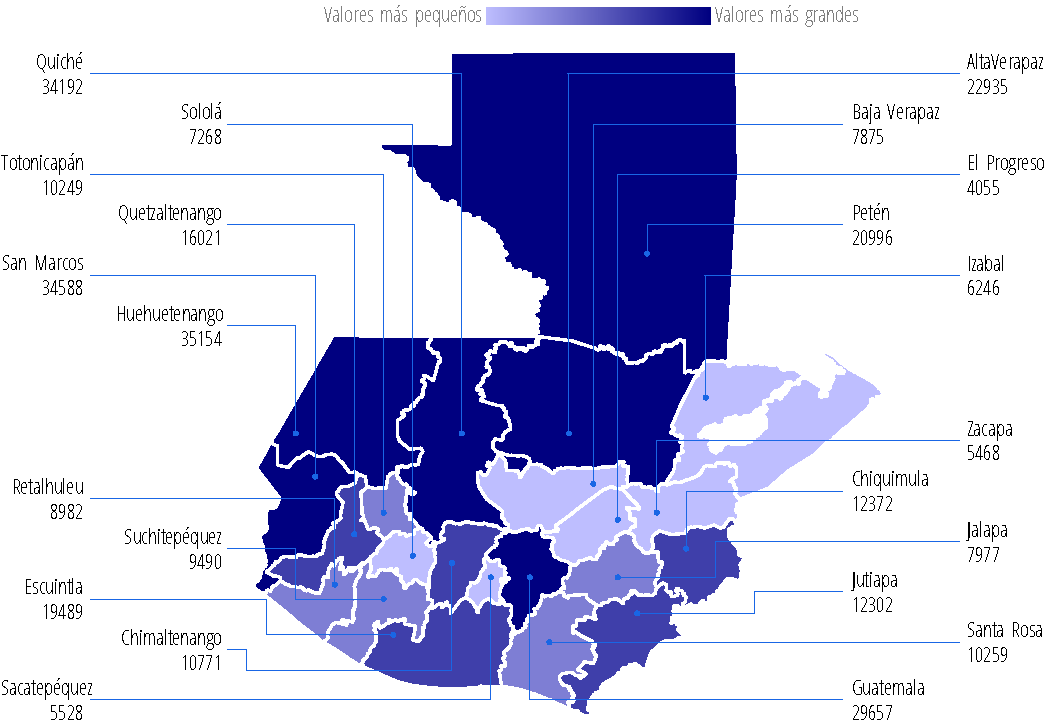
\includegraphics[width=52\cuadri]{graficas/5_14.pdf}}%
{%
	Sigsa} %


%#########################15########################

\cajita{%
	Infecciones respiratorias agudas}%
{%
	En el período de 2011  a 2015 la menor cantidad de Infecciones respiratorias agudas que fueron atendidas por personal médico se registró en 2015, siendo un total de 1,184,756.
}%
{%
	Niños menores de cinco años que recibieron atención médica por infecciones respiratorias agudas} %
{%
	República de Guatemala, serie histórica, número de niños} %
{%
	\begin{tikzpicture}[x=1pt,y=1pt]  % Created by tikzDevice version 0.9 on 2016-03-03 05:26:40
% !TEX encoding = UTF-8 Unicode
\definecolor{fillColor}{RGB}{255,255,255}
\path[use as bounding box,fill=fillColor,fill opacity=0.00] (0,0) rectangle (289.08,198.74);
\begin{scope}
\path[clip] (  0.00,  0.00) rectangle (289.08,198.74);

\path[] (  0.00,  0.00) rectangle (289.08,198.74);
\end{scope}
\begin{scope}
\path[clip] (  0.00,  0.00) rectangle (289.08,198.74);

\path[] ( 21.38, 15.61) rectangle (280.54,191.48);

\path[] ( 21.38, 36.84) --
	(280.54, 36.84);

\path[] ( 21.38, 92.67) --
	(280.54, 92.67);

\path[] ( 21.38,148.50) --
	(280.54,148.50);

\path[] ( 21.38, 64.76) --
	(280.54, 64.76);

\path[] ( 21.38,120.58) --
	(280.54,120.58);

\path[] ( 21.38,176.41) --
	(280.54,176.41);

\path[] ( 51.28, 15.61) --
	( 51.28,191.48);

\path[] (101.12, 15.61) --
	(101.12,191.48);

\path[] (150.96, 15.61) --
	(150.96,191.48);

\path[] (200.80, 15.61) --
	(200.80,191.48);

\path[] (250.64, 15.61) --
	(250.64,191.48);
\definecolor{drawColor}{RGB}{0,0,255}

\path[draw=drawColor,line width= 1.7pt,line join=round] ( 51.28, 66.18) --
	(101.12,107.14) --
	(150.96,183.49) --
	(200.80,147.27) --
	(250.64, 60.50);
\definecolor{drawColor}{RGB}{0,0,0}

\node[text=drawColor,anchor=base,inner sep=0pt, outer sep=0pt, scale=  1.02] at ( 51.28, 54.27) {1,205,111};

\node[text=drawColor,anchor=base east,inner sep=0pt, outer sep=0pt, scale=  1.02] at ( 93.97,107.14) {1,351,837};

\node[text=drawColor,anchor=base,inner sep=0pt, outer sep=0pt, scale=  1.02] at (150.96,187.46) {1,625,358};

\node[text=drawColor,anchor=base west,inner sep=0pt, outer sep=0pt, scale=  1.02] at (200.80,151.24) {1,495,601};

\node[text=drawColor,anchor=base,inner sep=0pt, outer sep=0pt, scale=  1.02] at (250.64, 48.59) {1,184,756};

\path[draw=drawColor,line width= 0.1pt,line join=round] ( 21.38, 23.61) -- (280.54, 23.61);

\path[] ( 21.38, 15.61) rectangle (280.54,191.48);
\end{scope}
\begin{scope}
\path[clip] (  0.00,  0.00) rectangle (289.08,198.74);

\path[] ( 21.38, 15.61) --
	( 21.38,191.48);
\end{scope}
\begin{scope}
\path[clip] (  0.00,  0.00) rectangle (289.08,198.74);
\definecolor{drawColor}{RGB}{255,255,255}

\node[text=drawColor,text opacity=0.00,anchor=base east,inner sep=0pt, outer sep=0pt, scale=  1.00] at ( 16.43, 60.85) {1200000};

\node[text=drawColor,text opacity=0.00,anchor=base east,inner sep=0pt, outer sep=0pt, scale=  1.00] at ( 16.43,116.68) {1400000};

\node[text=drawColor,text opacity=0.00,anchor=base east,inner sep=0pt, outer sep=0pt, scale=  1.00] at ( 16.43,172.50) {1600000};
\end{scope}
\begin{scope}
\path[clip] (  0.00,  0.00) rectangle (289.08,198.74);

\path[] ( 18.63, 64.76) --
	( 21.38, 64.76);

\path[] ( 18.63,120.58) --
	( 21.38,120.58);

\path[] ( 18.63,176.41) --
	( 21.38,176.41);
\end{scope}
\begin{scope}
\path[clip] (  0.00,  0.00) rectangle (289.08,198.74);

\path[] ( 21.38, 15.61) --
	(280.54, 15.61);
\end{scope}
\begin{scope}
\path[clip] (  0.00,  0.00) rectangle (289.08,198.74);

\path[] ( 51.28, 12.86) --
	( 51.28, 15.61);

\path[] (101.12, 12.86) --
	(101.12, 15.61);

\path[] (150.96, 12.86) --
	(150.96, 15.61);

\path[] (200.80, 12.86) --
	(200.80, 15.61);

\path[] (250.64, 12.86) --
	(250.64, 15.61);
\end{scope}
\begin{scope}
\path[clip] (  0.00,  0.00) rectangle (289.08,198.74);
\definecolor{drawColor}{RGB}{0,0,0}

\node[text=drawColor,anchor=base,inner sep=0pt, outer sep=0pt, scale=  1.00] at ( 51.28,  2.85) {2011};

\node[text=drawColor,anchor=base,inner sep=0pt, outer sep=0pt, scale=  1.00] at (101.12,  2.85) {2012};

\node[text=drawColor,anchor=base,inner sep=0pt, outer sep=0pt, scale=  1.00] at (150.96,  2.85) {2013};

\node[text=drawColor,anchor=base,inner sep=0pt, outer sep=0pt, scale=  1.00] at (200.80,  2.85) {2014};

\node[text=drawColor,anchor=base,inner sep=0pt, outer sep=0pt, scale=  1.00] at (250.64,  2.85) {2015};
\end{scope}
  \end{tikzpicture}}%
{%
	Sigsa} %

%#########################16########################

\cajita{%
	Infecciones respiratorias agudas según sexo}%
{%
	Al igual que en el caso de la atención por diarreas, la cantidad de casos de IRA atendidos por personal médico es muy similar entre hombres y mujeres. 
}%
{%
	Niños menores de cinco años que recibieron atención médica por infecciones respiratorias agudas, según sexo} %
{%
	República de Guatemala, 2015, número de niños} %
{%
	\begin{tikzpicture}[x=1pt,y=1pt]  % Created by tikzDevice version 0.9 on 2016-03-03 05:26:47
% !TEX encoding = UTF-8 Unicode
\definecolor{fillColor}{RGB}{255,255,255}
\path[use as bounding box,fill=fillColor,fill opacity=0.00] (0,0) rectangle (289.08,198.74);
\begin{scope}
\path[clip] (  0.00,  0.00) rectangle (289.08,198.74);

\path[] (  0.00,  0.00) rectangle (289.08,198.74);
\end{scope}
\begin{scope}
\path[clip] (  0.00,  0.00) rectangle (289.08,198.74);

\path[] (  0.00, 12.77) rectangle (289.08,181.67);

\path[] ( 54.20, 12.77) --
	( 54.20,181.67);

\path[] (144.54, 12.77) --
	(144.54,181.67);

\path[] (234.88, 12.77) --
	(234.88,181.67);
\definecolor{drawColor}{RGB}{0,0,255}
\definecolor{fillColor}{RGB}{0,0,255}

\path[draw=drawColor,line width= 0.6pt,line join=round,fill=fillColor] ( 36.13, 20.44) rectangle ( 72.27,173.99);

\path[draw=drawColor,line width= 0.6pt,line join=round,fill=fillColor] (126.47, 20.44) rectangle (162.61, 97.96);

\path[draw=drawColor,line width= 0.6pt,line join=round,fill=fillColor] (216.81, 20.44) rectangle (252.95, 96.48);
\definecolor{drawColor}{RGB}{0,0,0}

\path[draw=drawColor,line width= 0.1pt,line join=round] (  0.00, 20.44) -- (289.08, 20.44);

\node[text=drawColor,anchor=base,inner sep=0pt, outer sep=0pt, scale=  1.02] at ( 54.20,177.96) {1,184,756};

\node[text=drawColor,anchor=base,inner sep=0pt, outer sep=0pt, scale=  1.02] at (144.54,101.93) {598,090};

\node[text=drawColor,anchor=base,inner sep=0pt, outer sep=0pt, scale=  1.02] at (234.88,100.45) {586,666};

\path[] (  0.00, 12.77) rectangle (289.08,181.67);
\end{scope}
\begin{scope}
\path[clip] (  0.00,  0.00) rectangle (289.08,198.74);

\path[] (  0.00, 12.77) --
	(289.08, 12.77);
\end{scope}
\begin{scope}
\path[clip] (  0.00,  0.00) rectangle (289.08,198.74);

\path[] ( 54.20, 10.02) --
	( 54.20, 12.77);

\path[] (144.54, 10.02) --
	(144.54, 12.77);

\path[] (234.88, 10.02) --
	(234.88, 12.77);
\end{scope}
\begin{scope}
\path[clip] (  0.00,  0.00) rectangle (289.08,198.74);
\definecolor{drawColor}{RGB}{0,0,0}

\node[text=drawColor,anchor=base,inner sep=0pt, outer sep=0pt, scale=  1.00] at ( 54.20, -0.00) {Total};

\node[text=drawColor,anchor=base,inner sep=0pt, outer sep=0pt, scale=  1.00] at (144.54, -0.00) {Hombre};

\node[text=drawColor,anchor=base,inner sep=0pt, outer sep=0pt, scale=  1.00] at (234.88, -0.00) {Mujer};
\end{scope}
  \end{tikzpicture}}%
{%
	Sigsa} %

%#########################17########################

\cajota{%
	Casos de IRA por departamento}%
{%
	Los departamentos que registraron mayor cantidad de atención médica de casos de IRA fueron Guatemala (124,186), San Marcos (108,781) y Petén (98,928). 	Los departamentos con la menor cantidad de registros médicos de atención a casos de IRA fueron Zacapa (21,997), Sacatepéquez (20,614) y El Progreso (15,350). 
}%
{%
	Niños menores de cinco años que recibieron atención médica por infecciones respiratorias agudas por departamento} %
{%
	República de Guatemala, departamental, número de niños} %
{%
	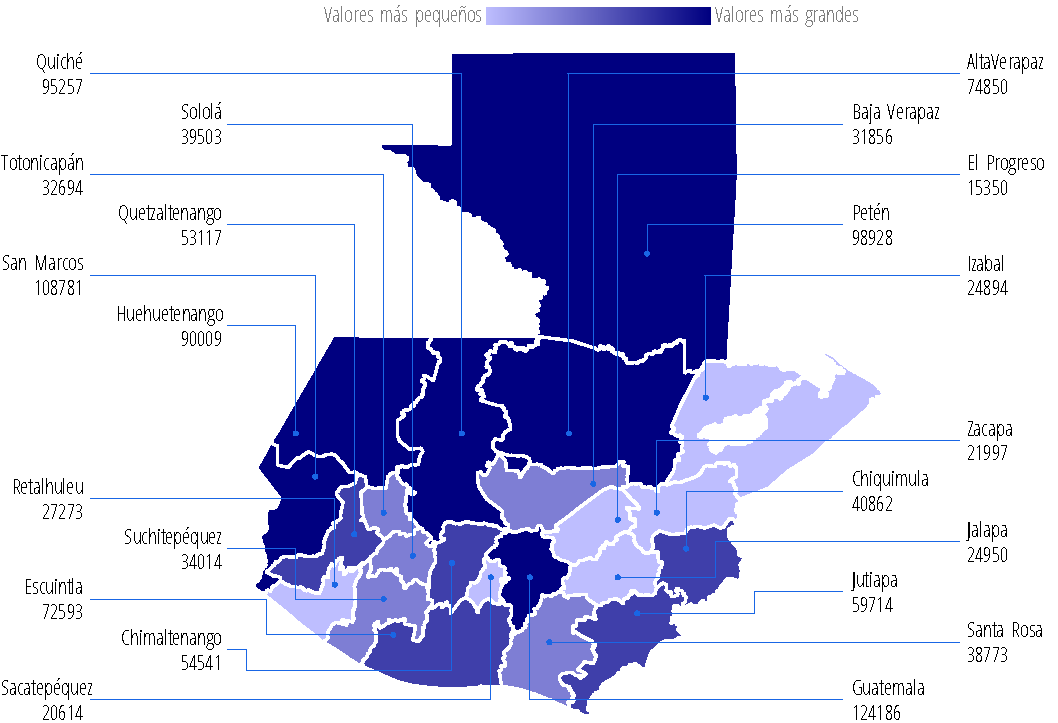
\includegraphics[width=52\cuadri]{graficas/5_17.pdf}}%
{%
	Sigsa} %



%#########################9########################

\cajita{%
	Asistencia prenatal}%
{%

En todos los grupos de edad, el porcentaje de mujeres que recibieron atención médica prenatal de un proveedor calificado es al menos del 90\%. 
}%
{%
	Mujeres que recibieron atención prenatal de un proveedor calificado, según grupos de edad} %
{%
	República de Guatemala, 2014, en porcentaje} %
{%
	\begin{tikzpicture}[x=1pt,y=1pt]  % Created by tikzDevice version 0.9 on 2016-03-03 05:26:15
% !TEX encoding = UTF-8 Unicode
\definecolor{fillColor}{RGB}{255,255,255}
\path[use as bounding box,fill=fillColor,fill opacity=0.00] (0,0) rectangle (289.08,198.74);
\begin{scope}
\path[clip] (  0.00,  0.00) rectangle (289.08,198.74);

\path[] (  0.00,  0.00) rectangle (289.08,198.74);
\end{scope}
\begin{scope}
\path[clip] (  0.00,  0.00) rectangle (289.08,198.74);

\path[] (  0.00, 12.77) rectangle (289.08,181.67);

\path[] ( 54.20, 12.77) --
	( 54.20,181.67);

\path[] (144.54, 12.77) --
	(144.54,181.67);

\path[] (234.88, 12.77) --
	(234.88,181.67);
\definecolor{drawColor}{RGB}{0,0,255}
\definecolor{fillColor}{RGB}{0,0,255}

\path[draw=drawColor,line width= 0.6pt,line join=round,fill=fillColor] ( 36.13, 20.44) rectangle ( 72.27,172.82);

\path[draw=drawColor,line width= 0.6pt,line join=round,fill=fillColor] (126.47, 20.44) rectangle (162.61,173.99);

\path[draw=drawColor,line width= 0.6pt,line join=round,fill=fillColor] (216.81, 20.44) rectangle (252.95,171.31);
\definecolor{drawColor}{RGB}{0,0,0}

\path[draw=drawColor,line width= 0.1pt,line join=round] (  0.00, 20.44) -- (289.08, 20.44);

\node[text=drawColor,anchor=base,inner sep=0pt, outer sep=0pt, scale=  1.02] at ( 54.20,176.79) {90.9};

\node[text=drawColor,anchor=base,inner sep=0pt, outer sep=0pt, scale=  1.02] at (144.54,177.96) {91.6};

\node[text=drawColor,anchor=base,inner sep=0pt, outer sep=0pt, scale=  1.02] at (234.88,175.28) {90.0};

\path[] (  0.00, 12.77) rectangle (289.08,181.67);
\end{scope}
\begin{scope}
\path[clip] (  0.00,  0.00) rectangle (289.08,198.74);

\path[] (  0.00, 12.77) --
	(289.08, 12.77);
\end{scope}
\begin{scope}
\path[clip] (  0.00,  0.00) rectangle (289.08,198.74);

\path[] ( 54.20, 10.02) --
	( 54.20, 12.77);

\path[] (144.54, 10.02) --
	(144.54, 12.77);

\path[] (234.88, 10.02) --
	(234.88, 12.77);
\end{scope}
\begin{scope}
\path[clip] (  0.00,  0.00) rectangle (289.08,198.74);
\definecolor{drawColor}{RGB}{0,0,0}

\node[text=drawColor,anchor=base,inner sep=0pt, outer sep=0pt, scale=  1.00] at ( 54.20, -0.00) {Menor a 20};

\node[text=drawColor,anchor=base,inner sep=0pt, outer sep=0pt, scale=  1.00] at (144.54, -0.00) {20-34};

\node[text=drawColor,anchor=base,inner sep=0pt, outer sep=0pt, scale=  1.00] at (234.88, -0.00) {35-49};
\end{scope}
  \end{tikzpicture}}%
{%
	Ensmi 2014} %

%#########################10########################

\cajita{%
	Asistencia en el parto}%
{%
	Siete de cada diez mujeres menores de 34 años reciben algún tipo de asistencia médica a la hora del parto, mientras que para mujeres mayores de 34 años este indicador baja a 6 de cada diez. 
}%
{%
	Mujeres que recibieron atención a la hora del parto  de un proveedor calificado, según grupos de edad} %
{%
	República de Guatemala, 2014, en porcentaje} %
{%
	\begin{tikzpicture}[x=1pt,y=1pt]  % Created by tikzDevice version 0.9 on 2016-03-03 05:26:19
% !TEX encoding = UTF-8 Unicode
\definecolor{fillColor}{RGB}{255,255,255}
\path[use as bounding box,fill=fillColor,fill opacity=0.00] (0,0) rectangle (289.08,198.74);
\begin{scope}
\path[clip] (  0.00,  0.00) rectangle (289.08,198.74);

\path[] (  0.00,  0.00) rectangle (289.08,198.74);
\end{scope}
\begin{scope}
\path[clip] (  0.00,  0.00) rectangle (289.08,198.74);

\path[] (  0.00, 12.77) rectangle (289.08,181.67);

\path[] ( 54.20, 12.77) --
	( 54.20,181.67);

\path[] (144.54, 12.77) --
	(144.54,181.67);

\path[] (234.88, 12.77) --
	(234.88,181.67);
\definecolor{drawColor}{RGB}{0,0,255}
\definecolor{fillColor}{RGB}{0,0,255}

\path[draw=drawColor,line width= 0.6pt,line join=round,fill=fillColor] ( 36.13, 20.44) rectangle ( 72.27,173.99);

\path[draw=drawColor,line width= 0.6pt,line join=round,fill=fillColor] (126.47, 20.44) rectangle (162.61,169.93);

\path[draw=drawColor,line width= 0.6pt,line join=round,fill=fillColor] (216.81, 20.44) rectangle (252.95,146.49);
\definecolor{drawColor}{RGB}{0,0,0}

\path[draw=drawColor,line width= 0.1pt,line join=round] (  0.00, 20.44) -- (289.08, 20.44);

\node[text=drawColor,anchor=base,inner sep=0pt, outer sep=0pt, scale=  1.02] at ( 54.20,177.96) {68.1};

\node[text=drawColor,anchor=base,inner sep=0pt, outer sep=0pt, scale=  1.02] at (144.54,173.91) {66.3};

\node[text=drawColor,anchor=base,inner sep=0pt, outer sep=0pt, scale=  1.02] at (234.88,150.46) {55.9};

\path[] (  0.00, 12.77) rectangle (289.08,181.67);
\end{scope}
\begin{scope}
\path[clip] (  0.00,  0.00) rectangle (289.08,198.74);

\path[] (  0.00, 12.77) --
	(289.08, 12.77);
\end{scope}
\begin{scope}
\path[clip] (  0.00,  0.00) rectangle (289.08,198.74);

\path[] ( 54.20, 10.02) --
	( 54.20, 12.77);

\path[] (144.54, 10.02) --
	(144.54, 12.77);

\path[] (234.88, 10.02) --
	(234.88, 12.77);
\end{scope}
\begin{scope}
\path[clip] (  0.00,  0.00) rectangle (289.08,198.74);
\definecolor{drawColor}{RGB}{0,0,0}

\node[text=drawColor,anchor=base,inner sep=0pt, outer sep=0pt, scale=  1.00] at ( 54.20, -0.00) {Menor a 20};

\node[text=drawColor,anchor=base,inner sep=0pt, outer sep=0pt, scale=  1.00] at (144.54, -0.00) {20-34};

\node[text=drawColor,anchor=base,inner sep=0pt, outer sep=0pt, scale=  1.00] at (234.88, -0.00) {35-49};
\end{scope}
  \end{tikzpicture}}%
{%
	Ensmi 2014} %



%#########################11########################

\cajita{%
	Niños que reciben alguna vacuna o desparasitante}%
{%
	El número de niños que recibe alguna vacuna o desparasitante aumentó en 2015 respecto al 2011. 
	
	El año que presentó mayor cantidad de niños desparasitados o vacunados fue  2012.
}%
{%
	Niños que reciben vacunas o desparasitantes} %
{%
	República de Guatemala, serie histórica, número de niños} %
{%
	\begin{tikzpicture}[x=1pt,y=1pt]  % Created by tikzDevice version 0.9 on 2016-03-03 05:26:22
% !TEX encoding = UTF-8 Unicode
\definecolor{fillColor}{RGB}{255,255,255}
\path[use as bounding box,fill=fillColor,fill opacity=0.00] (0,0) rectangle (289.08,198.74);
\begin{scope}
\path[clip] (  0.00,  0.00) rectangle (289.08,198.74);

\path[] (  0.00,  0.00) rectangle (289.08,198.74);
\end{scope}
\begin{scope}
\path[clip] (  0.00,  0.00) rectangle (289.08,198.74);

\path[] ( 21.38, 15.61) rectangle (280.54,191.48);

\path[] ( 21.38, 44.20) --
	(280.54, 44.20);

\path[] ( 21.38, 99.35) --
	(280.54, 99.35);

\path[] ( 21.38,154.49) --
	(280.54,154.49);

\path[] ( 21.38, 16.63) --
	(280.54, 16.63);

\path[] ( 21.38, 71.77) --
	(280.54, 71.77);

\path[] ( 21.38,126.92) --
	(280.54,126.92);

\path[] ( 21.38,182.06) --
	(280.54,182.06);

\path[] ( 51.28, 15.61) --
	( 51.28,191.48);

\path[] (101.12, 15.61) --
	(101.12,191.48);

\path[] (150.96, 15.61) --
	(150.96,191.48);

\path[] (200.80, 15.61) --
	(200.80,191.48);

\path[] (250.64, 15.61) --
	(250.64,191.48);
\definecolor{drawColor}{RGB}{0,0,255}

\path[draw=drawColor,line width= 1.7pt,line join=round] ( 51.28, 60.50) --
	(101.12,183.49) --
	(150.96,102.33) --
	(200.80, 99.78) --
	(250.64, 99.78);
\definecolor{drawColor}{RGB}{0,0,0}

\node[text=drawColor,anchor=base,inner sep=0pt, outer sep=0pt, scale=  1.02] at ( 51.28, 48.59) {2,897,786};

\node[text=drawColor,anchor=base,inner sep=0pt, outer sep=0pt, scale=  1.02] at (101.12,187.46) {4,012,987};

\node[text=drawColor,anchor=base west,inner sep=0pt, outer sep=0pt, scale=  1.02] at (150.96,106.30) {3,277,046};

\node[text=drawColor,anchor=base west,inner sep=0pt, outer sep=0pt, scale=  1.02] at (200.80,103.76) {3,253,982};

\node[text=drawColor,anchor=base,inner sep=0pt, outer sep=0pt, scale=  1.02] at (250.64, 87.87) {3,253,951};

\path[draw=drawColor,line width= 0.1pt,line join=round] ( 21.38, 23.61) -- (280.54, 23.61);

\path[] ( 21.38, 15.61) rectangle (280.54,191.48);
\end{scope}
\begin{scope}
\path[clip] (  0.00,  0.00) rectangle (289.08,198.74);

\path[] ( 21.38, 15.61) --
	( 21.38,191.48);
\end{scope}
\begin{scope}
\path[clip] (  0.00,  0.00) rectangle (289.08,198.74);
\definecolor{drawColor}{RGB}{255,255,255}

\node[text=drawColor,text opacity=0.00,anchor=base east,inner sep=0pt, outer sep=0pt, scale=  1.00] at ( 16.43, 12.73) {2500000};

\node[text=drawColor,text opacity=0.00,anchor=base east,inner sep=0pt, outer sep=0pt, scale=  1.00] at ( 16.43, 67.87) {3000000};

\node[text=drawColor,text opacity=0.00,anchor=base east,inner sep=0pt, outer sep=0pt, scale=  1.00] at ( 16.43,123.01) {3500000};

\node[text=drawColor,text opacity=0.00,anchor=base east,inner sep=0pt, outer sep=0pt, scale=  1.00] at ( 16.43,178.15) {4000000};
\end{scope}
\begin{scope}
\path[clip] (  0.00,  0.00) rectangle (289.08,198.74);

\path[] ( 18.63, 16.63) --
	( 21.38, 16.63);

\path[] ( 18.63, 71.77) --
	( 21.38, 71.77);

\path[] ( 18.63,126.92) --
	( 21.38,126.92);

\path[] ( 18.63,182.06) --
	( 21.38,182.06);
\end{scope}
\begin{scope}
\path[clip] (  0.00,  0.00) rectangle (289.08,198.74);

\path[] ( 21.38, 15.61) --
	(280.54, 15.61);
\end{scope}
\begin{scope}
\path[clip] (  0.00,  0.00) rectangle (289.08,198.74);

\path[] ( 51.28, 12.86) --
	( 51.28, 15.61);

\path[] (101.12, 12.86) --
	(101.12, 15.61);

\path[] (150.96, 12.86) --
	(150.96, 15.61);

\path[] (200.80, 12.86) --
	(200.80, 15.61);

\path[] (250.64, 12.86) --
	(250.64, 15.61);
\end{scope}
\begin{scope}
\path[clip] (  0.00,  0.00) rectangle (289.08,198.74);
\definecolor{drawColor}{RGB}{0,0,0}

\node[text=drawColor,anchor=base,inner sep=0pt, outer sep=0pt, scale=  1.00] at ( 51.28,  2.85) {2011};

\node[text=drawColor,anchor=base,inner sep=0pt, outer sep=0pt, scale=  1.00] at (101.12,  2.85) {2012};

\node[text=drawColor,anchor=base,inner sep=0pt, outer sep=0pt, scale=  1.00] at (150.96,  2.85) {2013};

\node[text=drawColor,anchor=base,inner sep=0pt, outer sep=0pt, scale=  1.00] at (200.80,  2.85) {2014};

\node[text=drawColor,anchor=base,inner sep=0pt, outer sep=0pt, scale=  1.00] at (250.64,  2.85) {2015};
\end{scope}
  \end{tikzpicture}}%
{%
	Sigsa} %

%#########################7########################

\cajita{%
	Tasa Global de Fecundidad}%
{%	
	La Tasa Global de Fecundidad (TGF) ha ido en descenso, ya que en 1995 se ubicó en 5.1, mientras que para el 2014 llegó a 3.1 niños por mujer. 
}%
{%
	Evolución de la tasa global de fecundidad} %
{%
	República de Guatemala, serie histórica, niños por mujer} %
{%
	\begin{tikzpicture}[x=1pt,y=1pt]  % Created by tikzDevice version 0.9 on 2016-03-03 05:26:08
% !TEX encoding = UTF-8 Unicode
\definecolor{fillColor}{RGB}{255,255,255}
\path[use as bounding box,fill=fillColor,fill opacity=0.00] (0,0) rectangle (289.08,198.74);
\begin{scope}
\path[clip] (  0.00,  0.00) rectangle (289.08,198.74);

\path[] (  0.00,  0.00) rectangle (289.08,198.74);
\end{scope}
\begin{scope}
\path[clip] (  0.00,  0.00) rectangle (289.08,198.74);

\path[] (  1.74, 15.61) rectangle (280.54,191.48);

\path[] (  1.74, 38.98) --
	(280.54, 38.98);

\path[] (  1.74, 69.73) --
	(280.54, 69.73);

\path[] (  1.74,100.47) --
	(280.54,100.47);

\path[] (  1.74,131.22) --
	(280.54,131.22);

\path[] (  1.74,161.97) --
	(280.54,161.97);

\path[] (  1.74, 23.61) --
	(280.54, 23.61);

\path[] (  1.74, 54.35) --
	(280.54, 54.35);

\path[] (  1.74, 85.10) --
	(280.54, 85.10);

\path[] (  1.74,115.85) --
	(280.54,115.85);

\path[] (  1.74,146.59) --
	(280.54,146.59);

\path[] (  1.74,177.34) --
	(280.54,177.34);

\path[] ( 41.57, 15.61) --
	( 41.57,191.48);

\path[] (107.95, 15.61) --
	(107.95,191.48);

\path[] (174.33, 15.61) --
	(174.33,191.48);

\path[] (240.71, 15.61) --
	(240.71,191.48);
\definecolor{drawColor}{RGB}{0,0,255}

\path[draw=drawColor,line width= 1.7pt,line join=round] ( 41.57,183.49) --
	(107.95,140.44) --
	(174.33, 91.25) --
	(240.71, 60.50);
\definecolor{drawColor}{RGB}{0,0,0}

\node[text=drawColor,anchor=base,inner sep=0pt, outer sep=0pt, scale=  1.02] at ( 41.57,187.46) {5.1};

\node[text=drawColor,anchor=base west,inner sep=0pt, outer sep=0pt, scale=  1.02] at (107.95,144.41) {4.4};

\node[text=drawColor,anchor=base west,inner sep=0pt, outer sep=0pt, scale=  1.02] at (174.33, 95.22) {3.6};

\node[text=drawColor,anchor=base,inner sep=0pt, outer sep=0pt, scale=  1.02] at (240.71, 48.59) {3.1};

\path[draw=drawColor,line width= 0.1pt,line join=round] (  1.74, 23.61) -- (280.54, 23.61);

\path[] (  1.74, 15.61) rectangle (280.54,191.48);
\end{scope}
\begin{scope}
\path[clip] (  0.00,  0.00) rectangle (289.08,198.74);

\path[] (  1.74, 15.61) --
	(  1.74,191.48);
\end{scope}
\begin{scope}
\path[clip] (  0.00,  0.00) rectangle (289.08,198.74);

\path[] (  0.00, 23.61) --
	(  1.74, 23.61);

\path[] (  0.00, 54.35) --
	(  1.74, 54.35);

\path[] (  0.00, 85.10) --
	(  1.74, 85.10);

\path[] (  0.00,115.85) --
	(  1.74,115.85);

\path[] (  0.00,146.59) --
	(  1.74,146.59);

\path[] (  0.00,177.34) --
	(  1.74,177.34);
\end{scope}
\begin{scope}
\path[clip] (  0.00,  0.00) rectangle (289.08,198.74);

\path[] (  1.74, 15.61) --
	(280.54, 15.61);
\end{scope}
\begin{scope}
\path[clip] (  0.00,  0.00) rectangle (289.08,198.74);

\path[] ( 41.57, 12.86) --
	( 41.57, 15.61);

\path[] (107.95, 12.86) --
	(107.95, 15.61);

\path[] (174.33, 12.86) --
	(174.33, 15.61);

\path[] (240.71, 12.86) --
	(240.71, 15.61);
\end{scope}
\begin{scope}
\path[clip] (  0.00,  0.00) rectangle (289.08,198.74);
\definecolor{drawColor}{RGB}{0,0,0}

\node[text=drawColor,anchor=base,inner sep=0pt, outer sep=0pt, scale=  1.00] at ( 41.57,  2.85) {1995};

\node[text=drawColor,anchor=base,inner sep=0pt, outer sep=0pt, scale=  1.00] at (107.95,  2.85) {2002};

\node[text=drawColor,anchor=base,inner sep=0pt, outer sep=0pt, scale=  1.00] at (174.33,  2.85) {2008-2009};

\node[text=drawColor,anchor=base,inner sep=0pt, outer sep=0pt, scale=  1.00] at (240.71,  2.85) {2014-2015};
\end{scope}
  \end{tikzpicture}}%
{%
	Ensmi 2014, 2008, 2002 y 1995} %

%#########################8########################

\cajita{%
	Tasa Global de Fecundidad, por área de residencia}%
{%
	Al analizar la Tasa Global de Fecundidad por área de residencia, se observa que las mujeres en el área rural tienen menos hijos que las del área rural, esto es 2.5 contra 3.7. 
}%
{%
	Tasa global de fecundidad por área de residencia} %
{%
	República de Guatemala, 2014, niños por mujer} %
{%
	\begin{tikzpicture}[x=1pt,y=1pt]  % Created by tikzDevice version 0.9 on 2016-03-03 05:26:13
% !TEX encoding = UTF-8 Unicode
\definecolor{fillColor}{RGB}{255,255,255}
\path[use as bounding box,fill=fillColor,fill opacity=0.00] (0,0) rectangle (289.08,198.74);
\begin{scope}
\path[clip] (  0.00,  0.00) rectangle (289.08,198.74);

\path[] (  0.00,  0.00) rectangle (289.08,198.74);
\end{scope}
\begin{scope}
\path[clip] (  0.00,  0.00) rectangle (289.08,198.74);

\path[] (  0.00, 12.77) rectangle (289.08,181.67);

\path[] ( 54.20, 12.77) --
	( 54.20,181.67);

\path[] (144.54, 12.77) --
	(144.54,181.67);

\path[] (234.88, 12.77) --
	(234.88,181.67);
\definecolor{drawColor}{RGB}{0,0,255}
\definecolor{fillColor}{RGB}{0,0,255}

\path[draw=drawColor,line width= 0.6pt,line join=round,fill=fillColor] ( 36.13, 20.44) rectangle ( 72.27,149.09);

\path[draw=drawColor,line width= 0.6pt,line join=round,fill=fillColor] (126.47, 20.44) rectangle (162.61,173.99);

\path[draw=drawColor,line width= 0.6pt,line join=round,fill=fillColor] (216.81, 20.44) rectangle (252.95,124.19);
\definecolor{drawColor}{RGB}{0,0,0}

\path[draw=drawColor,line width= 0.1pt,line join=round] (  0.00, 20.44) -- (289.08, 20.44);

\node[text=drawColor,anchor=base,inner sep=0pt, outer sep=0pt, scale=  1.02] at ( 54.20,153.06) {3.1};

\node[text=drawColor,anchor=base,inner sep=0pt, outer sep=0pt, scale=  1.02] at (144.54,177.96) {3.7};

\node[text=drawColor,anchor=base,inner sep=0pt, outer sep=0pt, scale=  1.02] at (234.88,128.16) {2.5};

\path[] (  0.00, 12.77) rectangle (289.08,181.67);
\end{scope}
\begin{scope}
\path[clip] (  0.00,  0.00) rectangle (289.08,198.74);

\path[] (  0.00, 12.77) --
	(289.08, 12.77);
\end{scope}
\begin{scope}
\path[clip] (  0.00,  0.00) rectangle (289.08,198.74);

\path[] ( 54.20, 10.02) --
	( 54.20, 12.77);

\path[] (144.54, 10.02) --
	(144.54, 12.77);

\path[] (234.88, 10.02) --
	(234.88, 12.77);
\end{scope}
\begin{scope}
\path[clip] (  0.00,  0.00) rectangle (289.08,198.74);
\definecolor{drawColor}{RGB}{0,0,0}

\node[text=drawColor,anchor=base,inner sep=0pt, outer sep=0pt, scale=  1.00] at ( 54.20, -0.00) {Total};

\node[text=drawColor,anchor=base,inner sep=0pt, outer sep=0pt, scale=  1.00] at (144.54, -0.00) {Urbana};

\node[text=drawColor,anchor=base,inner sep=0pt, outer sep=0pt, scale=  1.00] at (234.88, -0.00) {Rural};
\end{scope}
  \end{tikzpicture}}%
{%
	Ensmi 2014} %




%%%%%%%%%%%%%%%%%%%%%%%%%%%%%%%%%%13%%%%%%%%%%%%%%%%%%%%%%%%

\cajota{%
	Acceso a agua}%
{%
	
	Para el 2011, los departamentos en los cuales más del 50\% de los hogares rurales no contaban con la disponibilidad de agua potable fueron Alta Verapaz y Retalhuleu.}%
{%
	Proporción de hogares del área rural que no poseían acceso a agua potable
} %
{%
	Por departamento, año 2011, en porcentaje} %
{%
	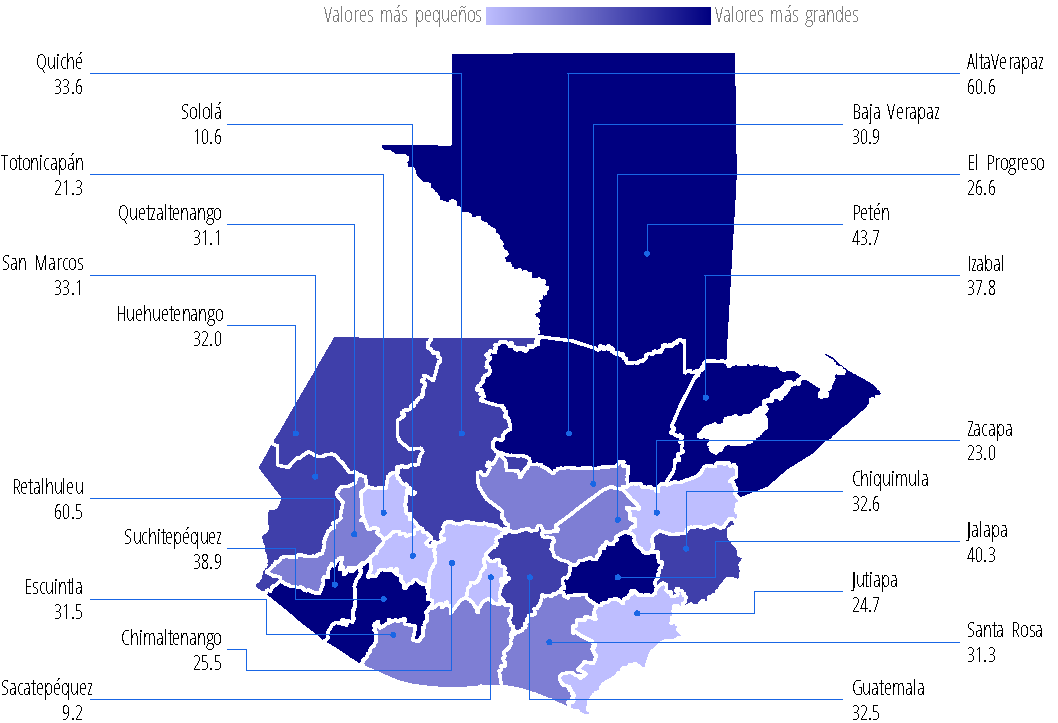
\includegraphics[width=52\cuadri]{graficas/1_14.pdf}}%
{%
	Instituto Nacional de Estadística (INE), Censos Municipales 2008 - 2011.} %




%%%%%%%%%%%%%%%%%%%%%%%%%%%%%%%%%%14%%%%%%%%%%%%%%%%%%%%%%%%

\cajota{%
	Acceso a servicios de saneamiento}%
{%
	Esta necesidad básica clasificada en el acceso a servicios sanitarios, tomas las variables de la Encuesta Nacional de Condiciones de Vida que recoge datos sobre la disponibilidad de servicios sanitarios y sistemas de eliminación de excretas.
	
	Para el 2011, el 40.4\% de los hogares rurales en Chiquimula no contaba con acceso a servicios de saneamiento, y en Jutiapa, Petén y Jalapa, tres de cada diez hogares del área rural también carecían de este servicio.   }%
{%
	Proporción de hogares del área rural sin acceso a servicios de saneamiento }
{%
	Por departamento, año 2011, en porcentaje} %
{%
	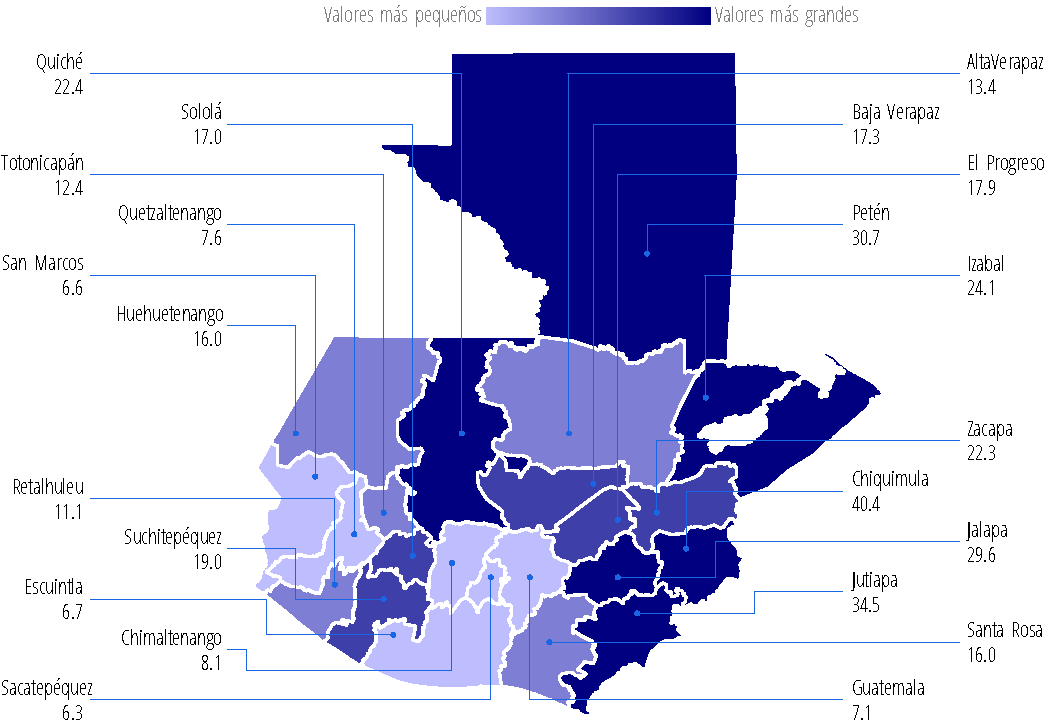
\includegraphics[width=52\cuadri]{graficas/1_15.pdf}}%
{%
	Instituto Nacional de Estadística (INE), Censos Municipales 2008 - 2011. } %


%#########################5########################

\cajita{%
	Viviendas y acceso al agua}%
{%
	Para el 2014, el 78.1\% de los hogares contaba con acceso a agua. A pesar de esto se presentan diferencias significativas entre el área rural y el área urbana, teniendo menor acceso esta última.
}%
{%
	Viviendas que tienen acceso a agua, según área de residencia} %
{%
	República de Guatemala, 2014, en porcentaje} %
{%
	\begin{tikzpicture}[x=1pt,y=1pt]  % Created by tikzDevice version 0.9 on 2016-03-03 05:26:02
% !TEX encoding = UTF-8 Unicode
\definecolor{fillColor}{RGB}{255,255,255}
\path[use as bounding box,fill=fillColor,fill opacity=0.00] (0,0) rectangle (289.08,198.74);
\begin{scope}
\path[clip] (  0.00,  0.00) rectangle (289.08,198.74);

\path[] (  0.00,  0.00) rectangle (289.08,198.74);
\end{scope}
\begin{scope}
\path[clip] (  0.00,  0.00) rectangle (289.08,198.74);

\path[] (  0.00, 12.77) rectangle (289.08,181.67);

\path[] ( 54.20, 12.77) --
	( 54.20,181.67);

\path[] (144.54, 12.77) --
	(144.54,181.67);

\path[] (234.88, 12.77) --
	(234.88,181.67);
\definecolor{drawColor}{RGB}{0,0,255}
\definecolor{fillColor}{RGB}{0,0,255}

\path[draw=drawColor,line width= 0.6pt,line join=round,fill=fillColor] ( 36.13, 20.44) rectangle ( 72.27,153.99);

\path[draw=drawColor,line width= 0.6pt,line join=round,fill=fillColor] (126.47, 20.44) rectangle (162.61,173.99);

\path[draw=drawColor,line width= 0.6pt,line join=round,fill=fillColor] (216.81, 20.44) rectangle (252.95,130.22);
\definecolor{drawColor}{RGB}{0,0,0}

\path[draw=drawColor,line width= 0.1pt,line join=round] (  0.00, 20.44) -- (289.08, 20.44);

\node[text=drawColor,anchor=base,inner sep=0pt, outer sep=0pt, scale=  1.02] at ( 54.20,157.96) {78.1};

\node[text=drawColor,anchor=base,inner sep=0pt, outer sep=0pt, scale=  1.02] at (144.54,177.96) {89.8};

\node[text=drawColor,anchor=base,inner sep=0pt, outer sep=0pt, scale=  1.02] at (234.88,134.19) {64.2};

\path[] (  0.00, 12.77) rectangle (289.08,181.67);
\end{scope}
\begin{scope}
\path[clip] (  0.00,  0.00) rectangle (289.08,198.74);

\path[] (  0.00, 12.77) --
	(289.08, 12.77);
\end{scope}
\begin{scope}
\path[clip] (  0.00,  0.00) rectangle (289.08,198.74);

\path[] ( 54.20, 10.02) --
	( 54.20, 12.77);

\path[] (144.54, 10.02) --
	(144.54, 12.77);

\path[] (234.88, 10.02) --
	(234.88, 12.77);
\end{scope}
\begin{scope}
\path[clip] (  0.00,  0.00) rectangle (289.08,198.74);
\definecolor{drawColor}{RGB}{0,0,0}

\node[text=drawColor,anchor=base,inner sep=0pt, outer sep=0pt, scale=  1.00] at ( 54.20, -0.00) { Total};

\node[text=drawColor,anchor=base,inner sep=0pt, outer sep=0pt, scale=  1.00] at (144.54, -0.00) {Urbana};

\node[text=drawColor,anchor=base,inner sep=0pt, outer sep=0pt, scale=  1.00] at (234.88, -0.00) {Rural};
\end{scope}
  \end{tikzpicture}}%
{%
	Encovi 2014} %


%#########################6########################

\cajita{%
	Viviendas y acceso a drenajes}%
{%
	
	Para el 2014, en la República de Guatemala, el acceso a drenajes no alcanzaba el 50\%. Además, en el área rural apenas el 11.6\% usa drenajes. 
	
}%
{%
	Viviendas que tienen acceso a drenajes según area de residencia} %
{%
	República de Guatemala, 2014, en porcentaje} %
{%
	\begin{tikzpicture}[x=1pt,y=1pt]  % Created by tikzDevice version 0.9 on 2016-03-03 05:26:05
% !TEX encoding = UTF-8 Unicode
\definecolor{fillColor}{RGB}{255,255,255}
\path[use as bounding box,fill=fillColor,fill opacity=0.00] (0,0) rectangle (289.08,198.74);
\begin{scope}
\path[clip] (  0.00,  0.00) rectangle (289.08,198.74);

\path[] (  0.00,  0.00) rectangle (289.08,198.74);
\end{scope}
\begin{scope}
\path[clip] (  0.00,  0.00) rectangle (289.08,198.74);

\path[] (  0.00, 12.77) rectangle (289.08,181.67);

\path[] ( 54.20, 12.77) --
	( 54.20,181.67);

\path[] (144.54, 12.77) --
	(144.54,181.67);

\path[] (234.88, 12.77) --
	(234.88,181.67);
\definecolor{drawColor}{RGB}{0,0,255}
\definecolor{fillColor}{RGB}{0,0,255}

\path[draw=drawColor,line width= 0.6pt,line join=round,fill=fillColor] ( 36.13, 20.44) rectangle ( 72.27,115.00);

\path[draw=drawColor,line width= 0.6pt,line join=round,fill=fillColor] (126.47, 20.44) rectangle (162.61,173.99);

\path[draw=drawColor,line width= 0.6pt,line join=round,fill=fillColor] (216.81, 20.44) rectangle (252.95, 44.71);
\definecolor{drawColor}{RGB}{0,0,0}

\path[draw=drawColor,line width= 0.1pt,line join=round] (  0.00, 20.44) -- (289.08, 20.44);

\node[text=drawColor,anchor=base,inner sep=0pt, outer sep=0pt, scale=  1.02] at ( 54.20,118.97) {45.2};

\node[text=drawColor,anchor=base,inner sep=0pt, outer sep=0pt, scale=  1.02] at (144.54,177.96) {73.4};

\node[text=drawColor,anchor=base,inner sep=0pt, outer sep=0pt, scale=  1.02] at (234.88, 48.68) {11.6};

\path[] (  0.00, 12.77) rectangle (289.08,181.67);
\end{scope}
\begin{scope}
\path[clip] (  0.00,  0.00) rectangle (289.08,198.74);

\path[] (  0.00, 12.77) --
	(289.08, 12.77);
\end{scope}
\begin{scope}
\path[clip] (  0.00,  0.00) rectangle (289.08,198.74);

\path[] ( 54.20, 10.02) --
	( 54.20, 12.77);

\path[] (144.54, 10.02) --
	(144.54, 12.77);

\path[] (234.88, 10.02) --
	(234.88, 12.77);
\end{scope}
\begin{scope}
\path[clip] (  0.00,  0.00) rectangle (289.08,198.74);
\definecolor{drawColor}{RGB}{0,0,0}

\node[text=drawColor,anchor=base,inner sep=0pt, outer sep=0pt, scale=  1.00] at ( 54.20, -0.00) {Total};

\node[text=drawColor,anchor=base,inner sep=0pt, outer sep=0pt, scale=  1.00] at (144.54, -0.00) {Urbana};

\node[text=drawColor,anchor=base,inner sep=0pt, outer sep=0pt, scale=  1.00] at (234.88, -0.00) {Rural};
\end{scope}
  \end{tikzpicture}}%
{%
	Encovi 2014} %



%#########################1########################

 \cajita{%
Viviendas formales }%
{%
	En la República, el 91.4\% de los hogares que no son pobres tiene una vivienda formal, mientras que cerca del 20\%  de los hogares que está en pobreza extrema no cuenta con una vivienda formal.  
 }%
{%
 Hogares con viviendas formales, según tipo de pobreza} %
{%
 República de Guatemala, 2014, en porcentaje} %
{%
 \begin{tikzpicture}[x=1pt,y=1pt]  % Created by tikzDevice version 0.9 on 2016-03-14 17:55:53
% !TEX encoding = UTF-8 Unicode
\definecolor{fillColor}{RGB}{255,255,255}
\path[use as bounding box,fill=fillColor,fill opacity=0.00] (0,0) rectangle (289.08,198.74);
\begin{scope}
\path[clip] (  0.00,  0.00) rectangle (289.08,198.74);

\path[] (  0.00,  0.00) rectangle (289.08,198.74);
\end{scope}
\begin{scope}
\path[clip] (  0.00,  0.00) rectangle (289.08,198.74);

\path[] (  0.00, 12.77) rectangle (289.08,181.67);

\path[] ( 54.20, 12.77) --
	( 54.20,181.67);

\path[] (144.54, 12.77) --
	(144.54,181.67);

\path[] (234.88, 12.77) --
	(234.88,181.67);
\definecolor{drawColor}{RGB}{0,0,255}
\definecolor{fillColor}{RGB}{0,0,255}

\path[draw=drawColor,line width= 0.6pt,line join=round,fill=fillColor] ( 36.13, 20.44) rectangle ( 72.27,173.99);

\path[draw=drawColor,line width= 0.6pt,line join=round,fill=fillColor] (126.47, 20.44) rectangle (162.61,168.11);

\path[draw=drawColor,line width= 0.6pt,line join=round,fill=fillColor] (216.81, 20.44) rectangle (252.95,156.69);
\definecolor{drawColor}{RGB}{0,0,0}

\path[draw=drawColor,line width= 0.1pt,line join=round] (  0.00, 20.44) -- (289.08, 20.44);

\node[text=drawColor,anchor=base,inner sep=0pt, outer sep=0pt, scale=  1.02] at ( 54.20,177.96) {91.4};

\node[text=drawColor,anchor=base,inner sep=0pt, outer sep=0pt, scale=  1.02] at (144.54,172.08) {87.9};

\node[text=drawColor,anchor=base,inner sep=0pt, outer sep=0pt, scale=  1.02] at (234.88,160.66) {81.1};

\path[] (  0.00, 12.77) rectangle (289.08,181.67);
\end{scope}
\begin{scope}
\path[clip] (  0.00,  0.00) rectangle (289.08,198.74);

\path[] (  0.00, 12.77) --
	(289.08, 12.77);
\end{scope}
\begin{scope}
\path[clip] (  0.00,  0.00) rectangle (289.08,198.74);

\path[] ( 54.20, 10.02) --
	( 54.20, 12.77);

\path[] (144.54, 10.02) --
	(144.54, 12.77);

\path[] (234.88, 10.02) --
	(234.88, 12.77);
\end{scope}
\begin{scope}
\path[clip] (  0.00,  0.00) rectangle (289.08,198.74);
\definecolor{drawColor}{RGB}{0,0,0}

\node[text=drawColor,anchor=base,inner sep=0pt, outer sep=0pt, scale=  1.00] at ( 54.20, -0.00) {No pobreza};

\node[text=drawColor,anchor=base,inner sep=0pt, outer sep=0pt, scale=  1.00] at (144.54, -0.00) {Pobreza no extrema};

\node[text=drawColor,anchor=base,inner sep=0pt, outer sep=0pt, scale=  1.00] at (234.88, -0.00) {Pobreza Extrema};
\end{scope}
  \end{tikzpicture}}%
{%
 Encovi 2014} %



%%%%%%%%%%%%%%%%%%%%%%%%%%%%%%%%%%12%%%%%%%%%%%%%%%%%%%%%%%%

\cajota{%
	Hogares que viven en hacinamiento en los departamentos}%
{% 
	El hacinamiento toma las variables de la Encuesta Nacional de Condiciones de Vida que recogen información sobre el número de personas en el hogar y el número de cuartos de la vivienda. 	Los departamentos con mayor porcentaje de hogares en el área rural que vivían en hacinamiento en el 2011 fueron: Alta Verapaz (64.8\%), Quiché (59.9\%), Huehuetenango (54.6\%), San Marcos (54.6\%), Suchitepéquez (52.7\%), Izabal (52.5\%), Petén (51.4\%), y Jalapa (51.4\%). }%
{%
	Proporción de hogares del área rural que vive en hacinamiento
} %
{%
	Por departamento, año 2011, en porcentaje} %
{%
	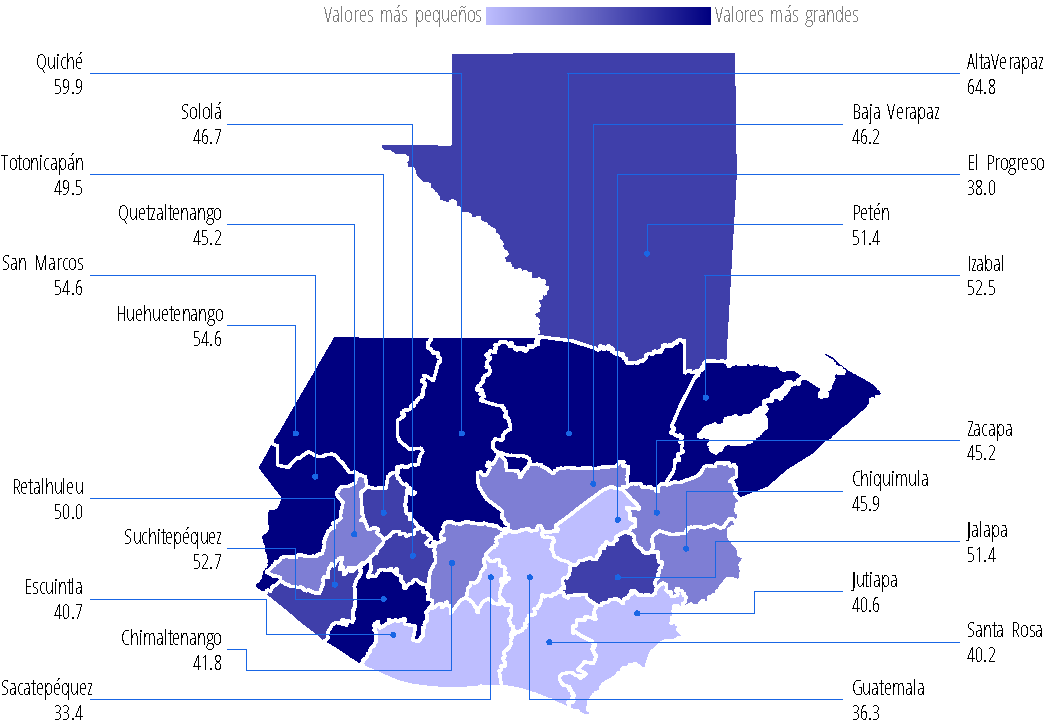
\includegraphics[width=52\cuadri]{graficas/1_13.pdf}}%
{%
 Encovi 2014} %


%#########################2########################

\cajita{%
	Viviendas con pared de block }%
{%
	Para el 2014, apenas el 22\% de los hogares en pobreza extrema tenía una vivienda con pared de block, mientras que los hogares que  no son pobres este indicador se ubicaba en 75.7\%. 
}%
{%
	Viviendas con pared de block, según tipo de pobreza} %
{%
	República de Guatemala, 2014, en porcentaje} %
{%
	\begin{tikzpicture}[x=1pt,y=1pt]  % Created by tikzDevice version 0.9 on 2016-03-14 17:57:53
% !TEX encoding = UTF-8 Unicode
\definecolor{fillColor}{RGB}{255,255,255}
\path[use as bounding box,fill=fillColor,fill opacity=0.00] (0,0) rectangle (289.08,198.74);
\begin{scope}
\path[clip] (  0.00,  0.00) rectangle (289.08,198.74);

\path[] (  0.00,  0.00) rectangle (289.08,198.74);
\end{scope}
\begin{scope}
\path[clip] (  0.00,  0.00) rectangle (289.08,198.74);

\path[] (  0.00, 12.77) rectangle (289.08,181.67);

\path[] ( 54.20, 12.77) --
	( 54.20,181.67);

\path[] (144.54, 12.77) --
	(144.54,181.67);

\path[] (234.88, 12.77) --
	(234.88,181.67);
\definecolor{drawColor}{RGB}{0,0,255}
\definecolor{fillColor}{RGB}{0,0,255}

\path[draw=drawColor,line width= 0.6pt,line join=round,fill=fillColor] ( 36.13, 20.44) rectangle ( 72.27,173.99);

\path[draw=drawColor,line width= 0.6pt,line join=round,fill=fillColor] (126.47, 20.44) rectangle (162.61,118.90);

\path[draw=drawColor,line width= 0.6pt,line join=round,fill=fillColor] (216.81, 20.44) rectangle (252.95, 65.03);
\definecolor{drawColor}{RGB}{0,0,0}

\path[draw=drawColor,line width= 0.1pt,line join=round] (  0.00, 20.44) -- (289.08, 20.44);

\node[text=drawColor,anchor=base,inner sep=0pt, outer sep=0pt, scale=  1.02] at ( 54.20,177.96) {75.7};

\node[text=drawColor,anchor=base,inner sep=0pt, outer sep=0pt, scale=  1.02] at (144.54,122.87) {48.5};

\node[text=drawColor,anchor=base,inner sep=0pt, outer sep=0pt, scale=  1.02] at (234.88, 69.00) {22.0};

\path[] (  0.00, 12.77) rectangle (289.08,181.67);
\end{scope}
\begin{scope}
\path[clip] (  0.00,  0.00) rectangle (289.08,198.74);

\path[] (  0.00, 12.77) --
	(289.08, 12.77);
\end{scope}
\begin{scope}
\path[clip] (  0.00,  0.00) rectangle (289.08,198.74);

\path[] ( 54.20, 10.02) --
	( 54.20, 12.77);

\path[] (144.54, 10.02) --
	(144.54, 12.77);

\path[] (234.88, 10.02) --
	(234.88, 12.77);
\end{scope}
\begin{scope}
\path[clip] (  0.00,  0.00) rectangle (289.08,198.74);
\definecolor{drawColor}{RGB}{0,0,0}

\node[text=drawColor,anchor=base,inner sep=0pt, outer sep=0pt, scale=  1.00] at ( 54.20, -0.00) {No pobreza};

\node[text=drawColor,anchor=base,inner sep=0pt, outer sep=0pt, scale=  1.00] at (144.54, -0.00) {Pobreza no extrema};

\node[text=drawColor,anchor=base,inner sep=0pt, outer sep=0pt, scale=  1.00] at (234.88, -0.00) {Pobreza Extrema};
\end{scope}
  \end{tikzpicture}}%
{%
	Encovi 2014} %

%#########################3########################

\cajita{%
	Viviendas con techo de lámina }%
{%
Los hogares que no son pobres utilizan en menor medida la lámina para la construcción del techo, con una diferencia cercana a los 25 puntos respecto a los hogares en pobreza extrema. 
	}%
{%
	Viviendas con techo de lámina,  según tipo de pobreza} %
{%
	República de Guatemala, 2014, en porcentaje} %
{%
	\begin{tikzpicture}[x=1pt,y=1pt]  % Created by tikzDevice version 0.9 on 2016-03-03 05:25:49
% !TEX encoding = UTF-8 Unicode
\definecolor{fillColor}{RGB}{255,255,255}
\path[use as bounding box,fill=fillColor,fill opacity=0.00] (0,0) rectangle (289.08,198.74);
\begin{scope}
\path[clip] (  0.00,  0.00) rectangle (289.08,198.74);

\path[] (  0.00,  0.00) rectangle (289.08,198.74);
\end{scope}
\begin{scope}
\path[clip] (  0.00,  0.00) rectangle (289.08,198.74);

\path[] ( -0.52, 15.61) rectangle (280.54,191.48);

\path[] (  0.00, 34.39) --
	(280.54, 34.39);

\path[] (  0.00, 62.22) --
	(280.54, 62.22);

\path[] (  0.00, 90.06) --
	(280.54, 90.06);

\path[] (  0.00,117.89) --
	(280.54,117.89);

\path[] (  0.00,145.72) --
	(280.54,145.72);

\path[] (  0.00,173.56) --
	(280.54,173.56);

\path[] (  0.00, 20.47) --
	(280.54, 20.47);

\path[] (  0.00, 48.31) --
	(280.54, 48.31);

\path[] (  0.00, 76.14) --
	(280.54, 76.14);

\path[] (  0.00,103.97) --
	(280.54,103.97);

\path[] (  0.00,131.81) --
	(280.54,131.81);

\path[] (  0.00,159.64) --
	(280.54,159.64);

\path[] (  0.00,187.47) --
	(280.54,187.47);

\path[] ( 52.18, 15.61) --
	( 52.18,191.48);

\path[] (140.01, 15.61) --
	(140.01,191.48);

\path[] (227.84, 15.61) --
	(227.84,191.48);
\definecolor{drawColor}{RGB}{0,0,255}

\path[draw=drawColor,line width= 1.7pt,line join=round] ( 52.18,183.49) --
	(140.01,172.52) --
	(227.84, 60.50);
\definecolor{drawColor}{RGB}{0,0,0}

\node[text=drawColor,anchor=base,inner sep=0pt, outer sep=0pt, scale=  1.02] at ( 52.18,187.46) {84.3};

\node[text=drawColor,anchor=base west,inner sep=0pt, outer sep=0pt, scale=  1.02] at (140.01,176.49) {82.3};

\node[text=drawColor,anchor=base,inner sep=0pt, outer sep=0pt, scale=  1.02] at (227.84, 48.59) {62.2};

\path[draw=drawColor,line width= 0.1pt,line join=round] (  0.00, 23.61) -- (280.54, 23.61);

\path[] ( -0.52, 15.61) rectangle (280.54,191.48);
\end{scope}
\begin{scope}
\path[clip] (  0.00,  0.00) rectangle (289.08,198.74);

\path[] (  0.00, 15.61) --
	(280.54, 15.61);
\end{scope}
\begin{scope}
\path[clip] (  0.00,  0.00) rectangle (289.08,198.74);

\path[] ( 52.18, 12.86) --
	( 52.18, 15.61);

\path[] (140.01, 12.86) --
	(140.01, 15.61);

\path[] (227.84, 12.86) --
	(227.84, 15.61);
\end{scope}
\begin{scope}
\path[clip] (  0.00,  0.00) rectangle (289.08,198.74);
\definecolor{drawColor}{RGB}{0,0,0}

\node[text=drawColor,anchor=base,inner sep=0pt, outer sep=0pt, scale=  1.00] at ( 52.18,  2.85) {Pobreza Extrema};

\node[text=drawColor,anchor=base,inner sep=0pt, outer sep=0pt, scale=  1.00] at (140.01,  2.85) {Pobreza no extrema};

\node[text=drawColor,anchor=base,inner sep=0pt, outer sep=0pt, scale=  1.00] at (227.84,  2.85) {No pobreza};
\end{scope}
  \end{tikzpicture}}%
{%
	Encovi 2014} %

%#########################4########################

\cajita{%
	Viviendas y material del piso}%
{%
	Los hogares en   pobreza extrema son los que presentan una menor proporción en el uso de torta de cemento (25.3\% contra un 67\%). Para los hogares que no son pobres predomina el uso de torta de cemento, ya que el 40.2\% de los hogares lo usa, contra un 10.4\% que usa piso de tierra. 
}%
{%
	Viviendas según material del piso y tipo de pobreza} %
{%
	República de Guatemala, 2014, en porcentaje} %
{%
	\begin{tikzpicture}[x=1pt,y=1pt]  % Created by tikzDevice version 0.9 on 2016-03-03 05:25:52
% !TEX encoding = UTF-8 Unicode
\definecolor{fillColor}{RGB}{255,255,255}
\path[use as bounding box,fill=fillColor,fill opacity=0.00] (0,0) rectangle (289.08,198.74);
\begin{scope}
\path[clip] (  0.00,  0.00) rectangle (289.08,198.74);

\path[] (  0.00,  0.00) rectangle (289.08,198.74);
\end{scope}
\begin{scope}
\path[clip] (  0.00,  0.00) rectangle (289.08,198.74);

\path[] (  0.00, 18.46) rectangle (289.08,166.57);

\path[] ( 54.20, 18.46) --
	( 54.20,166.57);

\path[] (144.54, 18.46) --
	(144.54,166.57);

\path[] (234.88, 18.46) --
	(234.88,166.57);
\definecolor{drawColor}{RGB}{0,0,255}
\definecolor{fillColor}{RGB}{0,0,255}

\path[draw=drawColor,line width= 0.6pt,line join=round,fill=fillColor] ( 15.81, 18.46) rectangle ( 51.94, 74.33);
\definecolor{drawColor}{RGB}{157,187,255}
\definecolor{fillColor}{RGB}{157,187,255}

\path[draw=drawColor,line width= 0.6pt,line join=round,fill=fillColor] ( 56.46, 18.46) rectangle ( 92.60,166.57);
\definecolor{drawColor}{RGB}{0,0,255}
\definecolor{fillColor}{RGB}{0,0,255}

\path[draw=drawColor,line width= 0.6pt,line join=round,fill=fillColor] (106.15, 18.46) rectangle (142.28,120.72);
\definecolor{drawColor}{RGB}{157,187,255}
\definecolor{fillColor}{RGB}{157,187,255}

\path[draw=drawColor,line width= 0.6pt,line join=round,fill=fillColor] (146.80, 18.46) rectangle (182.93, 95.86);
\definecolor{drawColor}{RGB}{0,0,255}
\definecolor{fillColor}{RGB}{0,0,255}

\path[draw=drawColor,line width= 0.6pt,line join=round,fill=fillColor] (196.48, 18.46) rectangle (232.62,107.27);
\definecolor{drawColor}{RGB}{157,187,255}
\definecolor{fillColor}{RGB}{157,187,255}

\path[draw=drawColor,line width= 0.6pt,line join=round,fill=fillColor] (237.14, 18.46) rectangle (273.27, 41.36);
\definecolor{drawColor}{RGB}{0,0,0}

\path[draw=drawColor,line width= 0.6pt,line join=round] (  0.00, 18.46) -- (289.08, 18.46);

\node[text=drawColor,rotate= 90.00,anchor=base west,inner sep=0pt, outer sep=0pt, scale=  0.83] at ( 37.11, 76.88) {25.3};

\node[text=drawColor,rotate= 90.00,anchor=base west,inner sep=0pt, outer sep=0pt, scale=  0.83] at ( 77.76,169.12) {67.0};

\node[text=drawColor,rotate= 90.00,anchor=base west,inner sep=0pt, outer sep=0pt, scale=  0.83] at (127.45,123.26) {46.3};

\node[text=drawColor,rotate= 90.00,anchor=base west,inner sep=0pt, outer sep=0pt, scale=  0.83] at (168.10, 98.40) {35.0};

\node[text=drawColor,rotate= 90.00,anchor=base west,inner sep=0pt, outer sep=0pt, scale=  0.83] at (217.79,109.81) {40.2};

\node[text=drawColor,rotate= 90.00,anchor=base west,inner sep=0pt, outer sep=0pt, scale=  0.83] at (258.44, 43.91) {10.4};

\path[] (  0.00, 18.46) rectangle (289.08,166.57);
\end{scope}
\begin{scope}
\path[clip] (  0.00,  0.00) rectangle (289.08,198.74);

\path[] (  0.00, 18.46) --
	(289.08, 18.46);
\end{scope}
\begin{scope}
\path[clip] (  0.00,  0.00) rectangle (289.08,198.74);

\path[] ( 54.20, 15.71) --
	( 54.20, 18.46);

\path[] (144.54, 15.71) --
	(144.54, 18.46);

\path[] (234.88, 15.71) --
	(234.88, 18.46);
\end{scope}
\begin{scope}
\path[clip] (  0.00,  0.00) rectangle (289.08,198.74);
\definecolor{drawColor}{RGB}{0,0,0}

\node[text=drawColor,anchor=base,inner sep=0pt, outer sep=0pt, scale=  1.00] at ( 54.20,  5.69) {Pobreza Extrema};

\node[text=drawColor,anchor=base,inner sep=0pt, outer sep=0pt, scale=  1.00] at (144.54,  5.69) {Pobreza no extrema};

\node[text=drawColor,anchor=base,inner sep=0pt, outer sep=0pt, scale=  1.00] at (234.88,  5.69) {No pobreza};
\end{scope}
\begin{scope}
\path[clip] (  0.00,  0.00) rectangle (289.08,198.74);
\coordinate (apoyo) at (41.26,191.13);
\coordinate (longitudFicticia) at (7.11,7.61);
\coordinate (longitud) at (7.11,7.11);
\coordinate (desX) at (157.45,0);
\coordinate (desY) at (0,0.25);
\definecolor[named]{ct1}{HTML}{
0000FF
}
\definecolor[named]{ct2}{HTML}{
9DBBFF
}
\definecolor[named]{ctb1}{HTML}{
0000FF
}
\definecolor[named]{ctb2}{HTML}{
9DBBFF
}
\path [fill=none] (apoyo) rectangle ($(apoyo)+(longitudFicticia)$)
node [xshift=0.3cm,inner sep=0pt, outer sep=0pt,midway,right,scale = 0.9]{Torta de cemento};
\draw [color = ctb1,fill=ct1] ( $(apoyo)  + (desY) $) rectangle ($(apoyo)+ (desY) +(longitud)$);
\path [fill=none] ($(apoyo)+(desX)$) rectangle ($(apoyo)+(desX)+(longitudFicticia)$)
node [xshift=0.3cm,inner sep=0pt, outer sep=0pt,midway,right,scale = 0.9]{Tierra};
\draw [color = ctb2 ,fill=ct2] ( $(apoyo)  + (desY) + (desX) $) rectangle ($(apoyo)+ (desY)+ (desX) +(longitud)$);
\end{scope}
  \end{tikzpicture}}%
{%
	Encovi 2014} %


%	\INEchaptercarta{Situación y atención a la desnutrición }{}
%	%#########################1########################

 \cajita{%
Mujeres con anemia }%
{%
	La salud de las madres debe ser monitoreada durante todo el período de gestación, para evitar futuros problemas en la salud tanto de la madre como del recién nacido. 
	
	Para el año 2008 se registró que del total de las madres embarazadas el 29.1\% padecía anemia\footnote{Síndrome que se caracteriza por la disminución anormal del número o tamaño de los glóbulos rojos que contiene la sangre o de su nivel de hemoglobina.}, mientras que en las mujeres que no se encontraban en gestación el porcentaje de anemia baja en 7.7 puntos porcentuales. 
 }%
{%
 Mujeres con anemia según estado de gestación} %
{%
 República de Guatemala, 2008-2009, en porcentaje} %
{%
 \begin{tikzpicture}[x=1pt,y=1pt]  % Created by tikzDevice version 0.9 on 2016-03-03 06:06:27
% !TEX encoding = UTF-8 Unicode
\definecolor{fillColor}{RGB}{255,255,255}
\path[use as bounding box,fill=fillColor,fill opacity=0.00] (0,0) rectangle (289.08,198.74);
\begin{scope}
\path[clip] (  0.00,  0.00) rectangle (289.08,198.74);

\path[] (  0.00,  0.00) rectangle (289.08,198.74);
\end{scope}
\begin{scope}
\path[clip] (  0.00,  0.00) rectangle (289.08,198.74);

\path[] (  0.00, 12.77) rectangle (289.08,181.67);

\path[] ( 78.84, 12.77) --
	( 78.84,181.67);

\path[] (210.24, 12.77) --
	(210.24,181.67);
\definecolor{drawColor}{RGB}{0,0,255}
\definecolor{fillColor}{RGB}{0,0,255}

\path[draw=drawColor,line width= 0.6pt,line join=round,fill=fillColor] ( 59.13, 20.44) rectangle ( 98.55,173.99);

\path[draw=drawColor,line width= 0.6pt,line join=round,fill=fillColor] (190.53, 20.44) rectangle (229.95,133.36);
\definecolor{drawColor}{RGB}{0,0,0}

\path[draw=drawColor,line width= 0.1pt,line join=round] (  0.00, 20.44) -- (289.08, 20.44);

\node[text=drawColor,anchor=base,inner sep=0pt, outer sep=0pt, scale=  1.02] at ( 78.84,177.96) {29.1};

\node[text=drawColor,anchor=base,inner sep=0pt, outer sep=0pt, scale=  1.02] at (210.24,137.33) {21.4};

\path[] (  0.00, 12.77) rectangle (289.08,181.67);
\end{scope}
\begin{scope}
\path[clip] (  0.00,  0.00) rectangle (289.08,198.74);

\path[] (  0.00, 12.77) --
	(289.08, 12.77);
\end{scope}
\begin{scope}
\path[clip] (  0.00,  0.00) rectangle (289.08,198.74);

\path[] ( 78.84, 10.02) --
	( 78.84, 12.77);

\path[] (210.24, 10.02) --
	(210.24, 12.77);
\end{scope}
\begin{scope}
\path[clip] (  0.00,  0.00) rectangle (289.08,198.74);
\definecolor{drawColor}{RGB}{0,0,0}

\node[text=drawColor,anchor=base,inner sep=0pt, outer sep=0pt, scale=  1.00] at ( 78.84, -0.00) {Embarazadas};

\node[text=drawColor,anchor=base,inner sep=0pt, outer sep=0pt, scale=  1.00] at (210.24, -0.00) {No embarazadas};
\end{scope}
  \end{tikzpicture}}%
{%
ENSMI 2008 } %

%#########################2########################

\cajita{%
	IMC }%
{%
	El índice de masa corporal (IMC)\footnote{$IMC = \frac{m}{a},
		 $ donde $m$ es la masa en kilogramos y $a$ la altura en metros.} es una medida de asociación entre la masa y la talla de un individuo ideada por el estadístico belga Adolphe Quetelet, por lo que también se conoce como índice de Quetelet.
		
		La mayoría de las mujeres guatemaltecas que no se encontraban embarazadas en el 2008 presentaban un IMC normal, mientras que solo un 1.6\% tenían IMC bajo. 
}%
{%
	Índice de masa corporal de mujeres no embarazadas} %
{%
	República de Guatemala, 2008-2009, en porcentaje} %
{%
	\begin{tikzpicture}[x=1pt,y=1pt]  % Created by tikzDevice version 0.9 on 2016-03-03 06:06:28
% !TEX encoding = UTF-8 Unicode
\definecolor{fillColor}{RGB}{255,255,255}
\path[use as bounding box,fill=fillColor,fill opacity=0.00] (0,0) rectangle (289.08,198.74);
\begin{scope}
\path[clip] (  0.00,  0.00) rectangle (289.08,198.74);

\path[] (  0.00,  0.00) rectangle (289.08,198.74);
\end{scope}
\begin{scope}
\path[clip] (  0.00,  0.00) rectangle (289.08,198.74);

\path[] (  0.00, 12.77) rectangle (289.08,181.67);

\path[] ( 41.30, 12.77) --
	( 41.30,181.67);

\path[] (110.13, 12.77) --
	(110.13,181.67);

\path[] (178.95, 12.77) --
	(178.95,181.67);

\path[] (247.78, 12.77) --
	(247.78,181.67);
\definecolor{drawColor}{RGB}{0,0,255}
\definecolor{fillColor}{RGB}{0,0,255}

\path[draw=drawColor,line width= 0.6pt,line join=round,fill=fillColor] ( 24.09, 20.44) rectangle ( 58.50, 25.57);

\path[draw=drawColor,line width= 0.6pt,line join=round,fill=fillColor] ( 92.92, 20.44) rectangle (127.33,173.99);

\path[draw=drawColor,line width= 0.6pt,line join=round,fill=fillColor] (161.75, 20.44) rectangle (196.16,132.96);

\path[draw=drawColor,line width= 0.6pt,line join=round,fill=fillColor] (230.58, 20.44) rectangle (264.99, 69.81);
\definecolor{drawColor}{RGB}{0,0,0}

\path[draw=drawColor,line width= 0.1pt,line join=round] (  0.00, 20.44) -- (289.08, 20.44);

\node[text=drawColor,anchor=base,inner sep=0pt, outer sep=0pt, scale=  1.02] at ( 41.30, 29.54) {1.6};

\node[text=drawColor,anchor=base,inner sep=0pt, outer sep=0pt, scale=  1.02] at (110.13,177.96) {47.9};

\node[text=drawColor,anchor=base,inner sep=0pt, outer sep=0pt, scale=  1.02] at (178.95,136.93) {35.1};

\node[text=drawColor,anchor=base,inner sep=0pt, outer sep=0pt, scale=  1.02] at (247.78, 73.78) {15.4};

\path[] (  0.00, 12.77) rectangle (289.08,181.67);
\end{scope}
\begin{scope}
\path[clip] (  0.00,  0.00) rectangle (289.08,198.74);

\path[] (  0.00, 12.77) --
	(289.08, 12.77);
\end{scope}
\begin{scope}
\path[clip] (  0.00,  0.00) rectangle (289.08,198.74);

\path[] ( 41.30, 10.02) --
	( 41.30, 12.77);

\path[] (110.13, 10.02) --
	(110.13, 12.77);

\path[] (178.95, 10.02) --
	(178.95, 12.77);

\path[] (247.78, 10.02) --
	(247.78, 12.77);
\end{scope}
\begin{scope}
\path[clip] (  0.00,  0.00) rectangle (289.08,198.74);
\definecolor{drawColor}{RGB}{0,0,0}

\node[text=drawColor,anchor=base,inner sep=0pt, outer sep=0pt, scale=  1.00] at ( 41.30, -0.00) {Bajo};

\node[text=drawColor,anchor=base,inner sep=0pt, outer sep=0pt, scale=  1.00] at (110.13, -0.00) {Normal};

\node[text=drawColor,anchor=base,inner sep=0pt, outer sep=0pt, scale=  1.00] at (178.95, -0.00) {Sobre peso};

\node[text=drawColor,anchor=base,inner sep=0pt, outer sep=0pt, scale=  1.00] at (247.78, -0.00) {Obesidad};
\end{scope}
  \end{tikzpicture}}%
{%
	ENSMI 2008} %


%#########################3########################

\cajita{%
	IMC según área de residencia }%
{%
	En el área urbana se presenta mayor proporción de de muejeres con sobre peso y obesidad (37.5\% y 20.3\%) que en el área rural. 
	
	Además el área rural presenta mayor proporción de mujeres con IMC normal que las del área urbana.  
	
	
}%
{%
	Índice de masa corporal de mujeres no embarazadas según área de residencia} %
{%
	República de Guatemala, 2008-2009, en porcentaje} %
{%
	\begin{tikzpicture}[x=1pt,y=1pt]  % Created by tikzDevice version 0.9 on 2016-03-03 06:06:32
% !TEX encoding = UTF-8 Unicode
\definecolor{fillColor}{RGB}{255,255,255}
\path[use as bounding box,fill=fillColor,fill opacity=0.00] (0,0) rectangle (289.08,198.74);
\begin{scope}
\path[clip] (  0.00,  0.00) rectangle (289.08,198.74);

\path[] (  0.00,  0.00) rectangle (289.08,198.74);
\end{scope}
\begin{scope}
\path[clip] (  0.00,  0.00) rectangle (289.08,198.74);

\path[] (  0.00, 18.46) rectangle (289.08,166.57);

\path[] ( 41.30, 18.46) --
	( 41.30,166.57);

\path[] (110.13, 18.46) --
	(110.13,166.57);

\path[] (178.95, 18.46) --
	(178.95,166.57);

\path[] (247.78, 18.46) --
	(247.78,166.57);
\definecolor{drawColor}{RGB}{0,0,255}
\definecolor{fillColor}{RGB}{0,0,255}

\path[draw=drawColor,line width= 0.6pt,line join=round,fill=fillColor] ( 12.05, 18.46) rectangle ( 39.58, 23.49);
\definecolor{drawColor}{RGB}{157,187,255}
\definecolor{fillColor}{RGB}{157,187,255}

\path[draw=drawColor,line width= 0.6pt,line join=round,fill=fillColor] ( 43.02, 18.46) rectangle ( 70.55, 22.65);
\definecolor{drawColor}{RGB}{0,0,255}
\definecolor{fillColor}{RGB}{0,0,255}

\path[draw=drawColor,line width= 0.6pt,line join=round,fill=fillColor] ( 80.87, 18.46) rectangle (108.40,131.64);
\definecolor{drawColor}{RGB}{157,187,255}
\definecolor{fillColor}{RGB}{157,187,255}

\path[draw=drawColor,line width= 0.6pt,line join=round,fill=fillColor] (111.85, 18.46) rectangle (139.38,166.57);
\definecolor{drawColor}{RGB}{0,0,255}
\definecolor{fillColor}{RGB}{0,0,255}

\path[draw=drawColor,line width= 0.6pt,line join=round,fill=fillColor] (149.70, 18.46) rectangle (177.23,123.26);
\definecolor{drawColor}{RGB}{157,187,255}
\definecolor{fillColor}{RGB}{157,187,255}

\path[draw=drawColor,line width= 0.6pt,line join=round,fill=fillColor] (180.68, 18.46) rectangle (208.21,111.80);
\definecolor{drawColor}{RGB}{0,0,255}
\definecolor{fillColor}{RGB}{0,0,255}

\path[draw=drawColor,line width= 0.6pt,line join=round,fill=fillColor] (218.53, 18.46) rectangle (246.06, 75.19);
\definecolor{drawColor}{RGB}{157,187,255}
\definecolor{fillColor}{RGB}{157,187,255}

\path[draw=drawColor,line width= 0.6pt,line join=round,fill=fillColor] (249.50, 18.46) rectangle (277.03, 52.27);
\definecolor{drawColor}{RGB}{0,0,0}

\path[draw=drawColor,line width= 0.6pt,line join=round] (  0.00, 18.46) -- (289.08, 18.46);

\node[text=drawColor,rotate= 90.00,anchor=base west,inner sep=0pt, outer sep=0pt, scale=  0.83] at ( 29.05, 25.31) {1.8};

\node[text=drawColor,rotate= 90.00,anchor=base west,inner sep=0pt, outer sep=0pt, scale=  0.83] at ( 60.02, 24.47) {1.5};

\node[text=drawColor,rotate= 90.00,anchor=base west,inner sep=0pt, outer sep=0pt, scale=  0.83] at ( 97.87,134.19) {40.5};

\node[text=drawColor,rotate= 90.00,anchor=base west,inner sep=0pt, outer sep=0pt, scale=  0.83] at (128.85,169.12) {53.0};

\node[text=drawColor,rotate= 90.00,anchor=base west,inner sep=0pt, outer sep=0pt, scale=  0.83] at (166.70,125.81) {37.5};

\node[text=drawColor,rotate= 90.00,anchor=base west,inner sep=0pt, outer sep=0pt, scale=  0.83] at (197.68,114.35) {33.4};

\node[text=drawColor,rotate= 90.00,anchor=base west,inner sep=0pt, outer sep=0pt, scale=  0.83] at (235.53, 77.74) {20.3};

\node[text=drawColor,rotate= 90.00,anchor=base west,inner sep=0pt, outer sep=0pt, scale=  0.83] at (266.50, 54.82) {12.1};

\path[] (  0.00, 18.46) rectangle (289.08,166.57);
\end{scope}
\begin{scope}
\path[clip] (  0.00,  0.00) rectangle (289.08,198.74);

\path[] (  0.00, 18.46) --
	(289.08, 18.46);
\end{scope}
\begin{scope}
\path[clip] (  0.00,  0.00) rectangle (289.08,198.74);

\path[] ( 41.30, 15.71) --
	( 41.30, 18.46);

\path[] (110.13, 15.71) --
	(110.13, 18.46);

\path[] (178.95, 15.71) --
	(178.95, 18.46);

\path[] (247.78, 15.71) --
	(247.78, 18.46);
\end{scope}
\begin{scope}
\path[clip] (  0.00,  0.00) rectangle (289.08,198.74);
\definecolor{drawColor}{RGB}{0,0,0}

\node[text=drawColor,anchor=base,inner sep=0pt, outer sep=0pt, scale=  1.00] at ( 41.30,  5.69) {Bajo};

\node[text=drawColor,anchor=base,inner sep=0pt, outer sep=0pt, scale=  1.00] at (110.13,  5.69) {Normal};

\node[text=drawColor,anchor=base,inner sep=0pt, outer sep=0pt, scale=  1.00] at (178.95,  5.69) {Sobre peso};

\node[text=drawColor,anchor=base,inner sep=0pt, outer sep=0pt, scale=  1.00] at (247.78,  5.69) {Obesidad};
\end{scope}
\begin{scope}
\path[clip] (  0.00,  0.00) rectangle (289.08,198.74);
\coordinate (apoyo) at (57.27,191.13);
\coordinate (longitudFicticia) at (7.11,7.61);
\coordinate (longitud) at (7.11,7.11);
\coordinate (desX) at (142.24,0);
\coordinate (desY) at (0,0.25);
\definecolor[named]{ct1}{HTML}{
0000FF
}
\definecolor[named]{ct2}{HTML}{
9DBBFF
}
\definecolor[named]{ctb1}{HTML}{
0000FF
}
\definecolor[named]{ctb2}{HTML}{
9DBBFF
}
\path [fill=none] (apoyo) rectangle ($(apoyo)+(longitudFicticia)$)
node [xshift=0.3cm,inner sep=0pt, outer sep=0pt,midway,right,scale = 0.9]{Urbana};
\draw [color = ctb1,fill=ct1] ( $(apoyo)  + (desY) $) rectangle ($(apoyo)+ (desY) +(longitud)$);
\path [fill=none] ($(apoyo)+(desX)$) rectangle ($(apoyo)+(desX)+(longitudFicticia)$)
node [xshift=0.3cm,inner sep=0pt, outer sep=0pt,midway,right,scale = 0.9]{Rural};
\draw [color = ctb2 ,fill=ct2] ( $(apoyo)  + (desY) + (desX) $) rectangle ($(apoyo)+ (desY)+ (desX) +(longitud)$);
\end{scope}
  \end{tikzpicture}}%
{%
	ENSMI 2008} %


%#########################4########################

\cajita{%
	Talla promedio según área de residencia }%
{%
	Para el 2008 la talla\footnote{Hace referencia a la estatura de una persona y en este caso se presenta en centímetros.} para madres de niños menores de 5 años es apenas mayor que la de las madres (de las mismas características) del área rural. 
}%
{%
	Talla promedio de madres  de niños menores de 5 años según área de residencia} %
{%
	República de Guatemala, 2008-2009, en centímetros} %
{%
	\begin{tikzpicture}[x=1pt,y=1pt]  % Created by tikzDevice version 0.9 on 2016-03-03 06:06:39
% !TEX encoding = UTF-8 Unicode
\definecolor{fillColor}{RGB}{255,255,255}
\path[use as bounding box,fill=fillColor,fill opacity=0.00] (0,0) rectangle (289.08,198.74);
\begin{scope}
\path[clip] (  0.00,  0.00) rectangle (289.08,198.74);

\path[] (  0.00,  0.00) rectangle (289.08,198.74);
\end{scope}
\begin{scope}
\path[clip] (  0.00,  0.00) rectangle (289.08,198.74);

\path[] (  0.00, 12.77) rectangle (289.08,181.67);

\path[] ( 78.84, 12.77) --
	( 78.84,181.67);

\path[] (210.24, 12.77) --
	(210.24,181.67);
\definecolor{drawColor}{RGB}{0,0,255}
\definecolor{fillColor}{RGB}{0,0,255}

\path[draw=drawColor,line width= 0.6pt,line join=round,fill=fillColor] ( 59.13, 20.44) rectangle ( 98.55,173.99);

\path[draw=drawColor,line width= 0.6pt,line join=round,fill=fillColor] (190.53, 20.44) rectangle (229.95,171.63);
\definecolor{drawColor}{RGB}{0,0,0}

\path[draw=drawColor,line width= 0.1pt,line join=round] (  0.00, 20.44) -- (289.08, 20.44);

\node[text=drawColor,anchor=base,inner sep=0pt, outer sep=0pt, scale=  1.02] at ( 78.84,177.96) {149.4};

\node[text=drawColor,anchor=base,inner sep=0pt, outer sep=0pt, scale=  1.02] at (210.24,175.60) {147.1};

\path[] (  0.00, 12.77) rectangle (289.08,181.67);
\end{scope}
\begin{scope}
\path[clip] (  0.00,  0.00) rectangle (289.08,198.74);

\path[] (  0.00, 12.77) --
	(289.08, 12.77);
\end{scope}
\begin{scope}
\path[clip] (  0.00,  0.00) rectangle (289.08,198.74);

\path[] ( 78.84, 10.02) --
	( 78.84, 12.77);

\path[] (210.24, 10.02) --
	(210.24, 12.77);
\end{scope}
\begin{scope}
\path[clip] (  0.00,  0.00) rectangle (289.08,198.74);
\definecolor{drawColor}{RGB}{0,0,0}

\node[text=drawColor,anchor=base,inner sep=0pt, outer sep=0pt, scale=  1.00] at ( 78.84, -0.00) {Urbana};

\node[text=drawColor,anchor=base,inner sep=0pt, outer sep=0pt, scale=  1.00] at (210.24, -0.00) {Rural};
\end{scope}
  \end{tikzpicture}}%
{%
	ENSMI 2008} %

%#########################5########################

\cajita{%
	Peso de niños recién nacidos }%
{%
	Uno de los datos más importantes que debe ser medido en un neonato es el peso. 
	
	Para el 2008 el 88.1\% de los recién nacidos presentaron un peso no menor de  2.5 kilogramos. 
}%
{%
	Distribución de niños recién nacidos según peso reportado por la madre} %
{%
	República de Guatemala, 2008-2009, en porcentaje} %
{%
	\begin{tikzpicture}[x=1pt,y=1pt]  % Created by tikzDevice version 0.9 on 2016-03-03 06:06:40
% !TEX encoding = UTF-8 Unicode
\definecolor{fillColor}{RGB}{255,255,255}
\path[use as bounding box,fill=fillColor,fill opacity=0.00] (0,0) rectangle (289.08,198.74);
\begin{scope}
\path[clip] (  0.00,  0.00) rectangle (289.08,198.74);

\path[] (  0.00,  0.00) rectangle (289.08,198.74);
\end{scope}
\begin{scope}
\path[clip] (  0.00,  0.00) rectangle (289.08,198.74);

\path[] (  0.00, 12.77) rectangle (289.08,181.67);

\path[] ( 54.20, 12.77) --
	( 54.20,181.67);

\path[] (144.54, 12.77) --
	(144.54,181.67);

\path[] (234.88, 12.77) --
	(234.88,181.67);
\definecolor{drawColor}{RGB}{0,0,255}
\definecolor{fillColor}{RGB}{0,0,255}

\path[draw=drawColor,line width= 0.6pt,line join=round,fill=fillColor] ( 36.13, 20.44) rectangle ( 72.27, 40.31);

\path[draw=drawColor,line width= 0.6pt,line join=round,fill=fillColor] (126.47, 20.44) rectangle (162.61,173.99);

\path[draw=drawColor,line width= 0.6pt,line join=round,fill=fillColor] (216.81, 20.44) rectangle (252.95, 21.32);
\definecolor{drawColor}{RGB}{0,0,0}

\path[draw=drawColor,line width= 0.1pt,line join=round] (  0.00, 20.44) -- (289.08, 20.44);

\node[text=drawColor,anchor=base,inner sep=0pt, outer sep=0pt, scale=  1.02] at ( 54.20, 44.28) {11.4};

\node[text=drawColor,anchor=base,inner sep=0pt, outer sep=0pt, scale=  1.02] at (144.54,177.96) {88.1};

\node[text=drawColor,anchor=base,inner sep=0pt, outer sep=0pt, scale=  1.02] at (234.88, 25.29) {0.5};

\path[] (  0.00, 12.77) rectangle (289.08,181.67);
\end{scope}
\begin{scope}
\path[clip] (  0.00,  0.00) rectangle (289.08,198.74);

\path[] (  0.00, 12.77) --
	(289.08, 12.77);
\end{scope}
\begin{scope}
\path[clip] (  0.00,  0.00) rectangle (289.08,198.74);

\path[] ( 54.20, 10.02) --
	( 54.20, 12.77);

\path[] (144.54, 10.02) --
	(144.54, 12.77);

\path[] (234.88, 10.02) --
	(234.88, 12.77);
\end{scope}
\begin{scope}
\path[clip] (  0.00,  0.00) rectangle (289.08,198.74);
\definecolor{drawColor}{RGB}{0,0,0}

\node[text=drawColor,anchor=base,inner sep=0pt, outer sep=0pt, scale=  1.00] at ( 54.20, -0.00) {Menos de 2.5 Kg};

\node[text=drawColor,anchor=base,inner sep=0pt, outer sep=0pt, scale=  1.00] at (144.54, -0.00) {2.5 Kg o más};

\node[text=drawColor,anchor=base,inner sep=0pt, outer sep=0pt, scale=  1.00] at (234.88, -0.00) {No sabe};
\end{scope}
  \end{tikzpicture}}%
{%
	ENSMI 2008} %

%#########################6########################

\cajita{%
	Desnutrición global }%
{%
	Durante los primeros años de vida de las niños se debe procurar un balance alimenticio para garantizar la salud de la niñez. 
	
	La tasa de desnutricion\footnote{Desnutrición es una deficiencia en la ingesta de calorías y proteínas, la cual, especialmente si es crónica, dificulta la salud y puede llevar a problemas en el desarrollo físico o intelectual que se pueden manifestar en diferentes problemas de adulto} global\footnote{La desnutrición global es  la deficiencia de peso para la edad} total para el 2008 fue de 13.1\%, siendo el 2.1\% desnutrición global severa. 
	
	
}%
{%
	Niños menores de 5 años con desnutrición global} %
{%
	República de Guatemala, 2008-2009, en porcentaje} %
{%
	\begin{tikzpicture}[x=1pt,y=1pt]  % Created by tikzDevice version 0.9 on 2016-03-03 06:06:44
% !TEX encoding = UTF-8 Unicode
\definecolor{fillColor}{RGB}{255,255,255}
\path[use as bounding box,fill=fillColor,fill opacity=0.00] (0,0) rectangle (289.08,198.74);
\begin{scope}
\path[clip] (  0.00,  0.00) rectangle (289.08,198.74);

\path[] (  0.00,  0.00) rectangle (289.08,198.74);
\end{scope}
\begin{scope}
\path[clip] (  0.00,  0.00) rectangle (289.08,198.74);

\path[] (  0.00, 12.77) rectangle (289.08,181.67);

\path[] ( 78.84, 12.77) --
	( 78.84,181.67);

\path[] (210.24, 12.77) --
	(210.24,181.67);
\definecolor{drawColor}{RGB}{0,0,255}
\definecolor{fillColor}{RGB}{0,0,255}

\path[draw=drawColor,line width= 0.6pt,line join=round,fill=fillColor] ( 59.13, 20.44) rectangle ( 98.55, 45.06);

\path[draw=drawColor,line width= 0.6pt,line join=round,fill=fillColor] (190.53, 20.44) rectangle (229.95,173.99);
\definecolor{drawColor}{RGB}{0,0,0}

\path[draw=drawColor,line width= 0.1pt,line join=round] (  0.00, 20.44) -- (289.08, 20.44);

\node[text=drawColor,anchor=base,inner sep=0pt, outer sep=0pt, scale=  1.02] at ( 78.84, 49.03) {2.1};

\node[text=drawColor,anchor=base,inner sep=0pt, outer sep=0pt, scale=  1.02] at (210.24,177.96) {13.1};

\path[] (  0.00, 12.77) rectangle (289.08,181.67);
\end{scope}
\begin{scope}
\path[clip] (  0.00,  0.00) rectangle (289.08,198.74);

\path[] (  0.00, 12.77) --
	(289.08, 12.77);
\end{scope}
\begin{scope}
\path[clip] (  0.00,  0.00) rectangle (289.08,198.74);

\path[] ( 78.84, 10.02) --
	( 78.84, 12.77);

\path[] (210.24, 10.02) --
	(210.24, 12.77);
\end{scope}
\begin{scope}
\path[clip] (  0.00,  0.00) rectangle (289.08,198.74);
\definecolor{drawColor}{RGB}{0,0,0}

\node[text=drawColor,anchor=base,inner sep=0pt, outer sep=0pt, scale=  1.00] at ( 78.84, -0.00) {Severa};

\node[text=drawColor,anchor=base,inner sep=0pt, outer sep=0pt, scale=  1.00] at (210.24, -0.00) {Total};
\end{scope}
  \end{tikzpicture}}%
{%
	ENSMI 2008} %

%#########################7########################

\cajita{%
	Desnutrición aguda }%
{%
	La desnutrición aguda se manifiesta por bajo peso en relación a la talla del individuo, el cual se origina por una situación reciente de falta de alimentos o una enfermedad que haya producido una pérdida rápida de peso. Este tipo de desnutrición es recuperable, sin embargo, de no ser atendida oportunamente pone en alto riesgo la vida del individuo.
	
	Este indicador se ubicó en 1.4\% para el 2008.
}%
{%
	Niños menores de 5 años con desnutrición aguda} %
{%
	República de Guatemala, 2008-2009, en porcentaje} %
{%
	\begin{tikzpicture}[x=1pt,y=1pt]  % Created by tikzDevice version 0.9 on 2016-03-03 06:06:45
% !TEX encoding = UTF-8 Unicode
\definecolor{fillColor}{RGB}{255,255,255}
\path[use as bounding box,fill=fillColor,fill opacity=0.00] (0,0) rectangle (289.08,198.74);
\begin{scope}
\path[clip] (  0.00,  0.00) rectangle (289.08,198.74);

\path[] (  0.00,  0.00) rectangle (289.08,198.74);
\end{scope}
\begin{scope}
\path[clip] (  0.00,  0.00) rectangle (289.08,198.74);

\path[] (  0.00, 12.77) rectangle (289.08,181.67);

\path[] ( 78.84, 12.77) --
	( 78.84,181.67);

\path[] (210.24, 12.77) --
	(210.24,181.67);
\definecolor{drawColor}{RGB}{0,0,255}
\definecolor{fillColor}{RGB}{0,0,255}

\path[draw=drawColor,line width= 0.6pt,line join=round,fill=fillColor] ( 59.13, 20.44) rectangle ( 98.55, 75.28);

\path[draw=drawColor,line width= 0.6pt,line join=round,fill=fillColor] (190.53, 20.44) rectangle (229.95,173.99);
\definecolor{drawColor}{RGB}{0,0,0}

\path[draw=drawColor,line width= 0.1pt,line join=round] (  0.00, 20.44) -- (289.08, 20.44);

\node[text=drawColor,anchor=base,inner sep=0pt, outer sep=0pt, scale=  1.02] at ( 78.84, 79.25) {0.5};

\node[text=drawColor,anchor=base,inner sep=0pt, outer sep=0pt, scale=  1.02] at (210.24,177.96) {1.4};

\path[] (  0.00, 12.77) rectangle (289.08,181.67);
\end{scope}
\begin{scope}
\path[clip] (  0.00,  0.00) rectangle (289.08,198.74);

\path[] (  0.00, 12.77) --
	(289.08, 12.77);
\end{scope}
\begin{scope}
\path[clip] (  0.00,  0.00) rectangle (289.08,198.74);

\path[] ( 78.84, 10.02) --
	( 78.84, 12.77);

\path[] (210.24, 10.02) --
	(210.24, 12.77);
\end{scope}
\begin{scope}
\path[clip] (  0.00,  0.00) rectangle (289.08,198.74);
\definecolor{drawColor}{RGB}{0,0,0}

\node[text=drawColor,anchor=base,inner sep=0pt, outer sep=0pt, scale=  1.00] at ( 78.84, -0.00) {Severa};

\node[text=drawColor,anchor=base,inner sep=0pt, outer sep=0pt, scale=  1.00] at (210.24, -0.00) {Total};
\end{scope}
  \end{tikzpicture}}%
{%
	ENSMI 2008} %


%#########################8########################

\cajita{%
	Desnutrición crónica }%
{%
	La desnutrición crónica es el retraso del crecimiento esperado para una edad. 
	
	Para niños menor de 5 años se observó en 2008 que el 49.8\% de estos presentan una talla menor a la esperada para su edad, es decir que se encontraban con desnutrición crónica. 
}%
{%
	Niños menores de 5 años con desnutrición crónica} %
{%
	República de Guatemala, 2008-2009, en porcentaje} %
{%
	\begin{tikzpicture}[x=1pt,y=1pt]  % Created by tikzDevice version 0.9 on 2016-03-03 06:18:20
% !TEX encoding = UTF-8 Unicode
\definecolor{fillColor}{RGB}{255,255,255}
\path[use as bounding box,fill=fillColor,fill opacity=0.00] (0,0) rectangle (289.08,198.74);
\begin{scope}
\path[clip] (  0.00,  0.00) rectangle (289.08,198.74);

\path[] (  0.00,  0.00) rectangle (289.08,198.74);
\end{scope}
\begin{scope}
\path[clip] (  0.00,  0.00) rectangle (289.08,198.74);

\path[] (  0.00, 12.77) rectangle (289.08,181.67);

\path[] ( 78.84, 12.77) --
	( 78.84,181.67);

\path[] (210.24, 12.77) --
	(210.24,181.67);
\definecolor{drawColor}{RGB}{0,0,255}
\definecolor{fillColor}{RGB}{0,0,255}

\path[draw=drawColor,line width= 0.6pt,line join=round,fill=fillColor] ( 59.13, 20.44) rectangle ( 98.55, 85.81);

\path[draw=drawColor,line width= 0.6pt,line join=round,fill=fillColor] (190.53, 20.44) rectangle (229.95,173.99);
\definecolor{drawColor}{RGB}{0,0,0}

\path[draw=drawColor,line width= 0.1pt,line join=round] (  0.00, 20.44) -- (289.08, 20.44);

\node[text=drawColor,anchor=base,inner sep=0pt, outer sep=0pt, scale=  1.02] at ( 78.84, 89.78) {21.2};

\node[text=drawColor,anchor=base,inner sep=0pt, outer sep=0pt, scale=  1.02] at (210.24,177.96) {49.8};

\path[] (  0.00, 12.77) rectangle (289.08,181.67);
\end{scope}
\begin{scope}
\path[clip] (  0.00,  0.00) rectangle (289.08,198.74);

\path[] (  0.00, 12.77) --
	(289.08, 12.77);
\end{scope}
\begin{scope}
\path[clip] (  0.00,  0.00) rectangle (289.08,198.74);

\path[] ( 78.84, 10.02) --
	( 78.84, 12.77);

\path[] (210.24, 10.02) --
	(210.24, 12.77);
\end{scope}
\begin{scope}
\path[clip] (  0.00,  0.00) rectangle (289.08,198.74);
\definecolor{drawColor}{RGB}{0,0,0}

\node[text=drawColor,anchor=base,inner sep=0pt, outer sep=0pt, scale=  1.00] at ( 78.84, -0.00) {Severa};

\node[text=drawColor,anchor=base,inner sep=0pt, outer sep=0pt, scale=  1.00] at (210.24, -0.00) {Total};
\end{scope}
  \end{tikzpicture}}%
{%
	ENSMI 2008} %


%#########################9########################

\cajita{%
	Niños con anemia }%
{%
	La pérdidad de peso, falta de producción de glóbulos rojos y aumento en la velocidad de destrucción de glóbulos rojos son las causas principales de la anemia. 
	
	Para la toma de políticas pública es imporante conocer la tasa de anemia en niños menores de 5 años. 
	
	El área rural presenta mayor porcentaje de niños con anemia ubicandose en 48.6\%, esto es 2.4 puntos por arriba del indicador para el área urbana. 
	
	}%
{%
	Niños entre 6 y 59 meses con anemia según área de residencia} %
{%
	República de Guatemala, 2008-2009, en porcentaje} %
{%
	\begin{tikzpicture}[x=1pt,y=1pt]  % Created by tikzDevice version 0.9 on 2016-03-03 06:06:46
% !TEX encoding = UTF-8 Unicode
\definecolor{fillColor}{RGB}{255,255,255}
\path[use as bounding box,fill=fillColor,fill opacity=0.00] (0,0) rectangle (289.08,198.74);
\begin{scope}
\path[clip] (  0.00,  0.00) rectangle (289.08,198.74);

\path[] (  0.00,  0.00) rectangle (289.08,198.74);
\end{scope}
\begin{scope}
\path[clip] (  0.00,  0.00) rectangle (289.08,198.74);

\path[] (  0.00, 12.77) rectangle (289.08,181.67);

\path[] ( 54.20, 12.77) --
	( 54.20,181.67);

\path[] (144.54, 12.77) --
	(144.54,181.67);

\path[] (234.88, 12.77) --
	(234.88,181.67);
\definecolor{drawColor}{RGB}{0,0,255}
\definecolor{fillColor}{RGB}{0,0,255}

\path[draw=drawColor,line width= 0.6pt,line join=round,fill=fillColor] ( 36.13, 20.44) rectangle ( 72.27,171.15);

\path[draw=drawColor,line width= 0.6pt,line join=round,fill=fillColor] (126.47, 20.44) rectangle (162.61,166.41);

\path[draw=drawColor,line width= 0.6pt,line join=round,fill=fillColor] (216.81, 20.44) rectangle (252.95,173.99);
\definecolor{drawColor}{RGB}{0,0,0}

\path[draw=drawColor,line width= 0.1pt,line join=round] (  0.00, 20.44) -- (289.08, 20.44);

\node[text=drawColor,anchor=base,inner sep=0pt, outer sep=0pt, scale=  1.02] at ( 54.20,175.12) {47.7};

\node[text=drawColor,anchor=base,inner sep=0pt, outer sep=0pt, scale=  1.02] at (144.54,170.38) {46.2};

\node[text=drawColor,anchor=base,inner sep=0pt, outer sep=0pt, scale=  1.02] at (234.88,177.96) {48.6};

\path[] (  0.00, 12.77) rectangle (289.08,181.67);
\end{scope}
\begin{scope}
\path[clip] (  0.00,  0.00) rectangle (289.08,198.74);

\path[] (  0.00, 12.77) --
	(289.08, 12.77);
\end{scope}
\begin{scope}
\path[clip] (  0.00,  0.00) rectangle (289.08,198.74);

\path[] ( 54.20, 10.02) --
	( 54.20, 12.77);

\path[] (144.54, 10.02) --
	(144.54, 12.77);

\path[] (234.88, 10.02) --
	(234.88, 12.77);
\end{scope}
\begin{scope}
\path[clip] (  0.00,  0.00) rectangle (289.08,198.74);
\definecolor{drawColor}{RGB}{0,0,0}

\node[text=drawColor,anchor=base,inner sep=0pt, outer sep=0pt, scale=  1.00] at ( 54.20, -0.00) {Total};

\node[text=drawColor,anchor=base,inner sep=0pt, outer sep=0pt, scale=  1.00] at (144.54, -0.00) {Urbana};

\node[text=drawColor,anchor=base,inner sep=0pt, outer sep=0pt, scale=  1.00] at (234.88, -0.00) {Rural};
\end{scope}
  \end{tikzpicture}}%
{%
	ENSMI 2008} %

%#########################9########################

\cajota{%
	Niños con anemia por departamento }%
{%
	El departamento de Suchitepéquez es el que presenta menor porcentaje de niños con anemia (37.7\%), seguido de El Progreso (37.8\%) y Quetzaltenango (40.2\%).
	
	Los departamentos con mayor porcentaje de anemia en niños son Totonicapán, Sololá y Chiquimula con 62.2\%, 56.1\% y 55.5\% respectivamente.  
	
	  
}%
{%
	Niños entre 6 y 59 meses con anemia por departamento} %
{%
	República de Guatemala, 2008-2009, en porcentaje} %
{%
	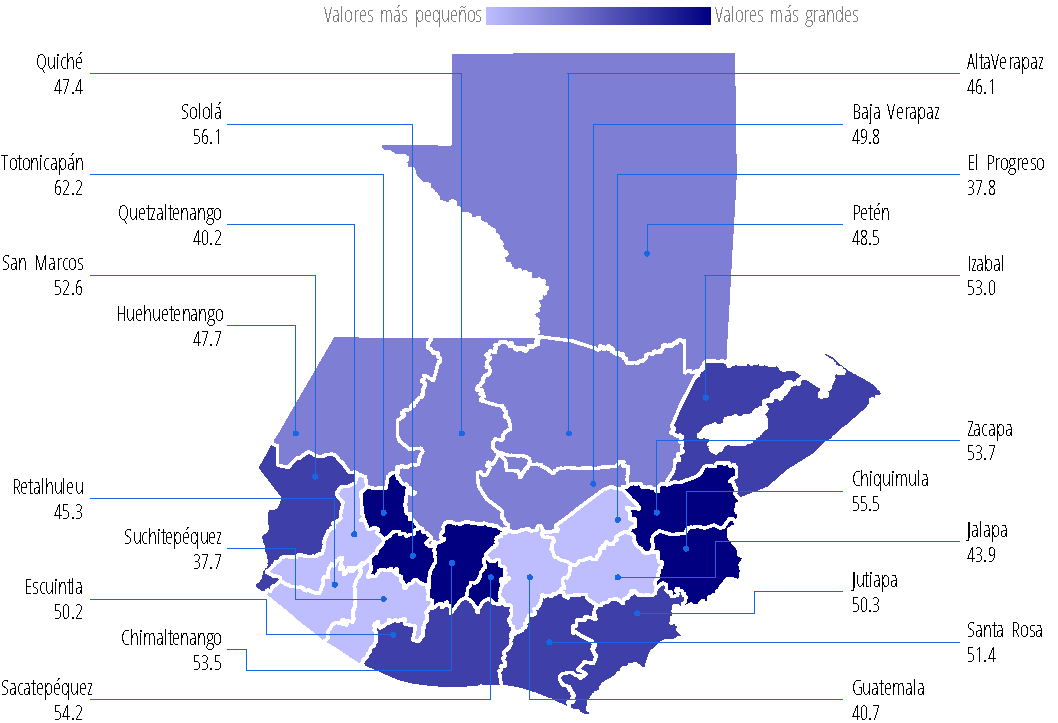
\includegraphics[width=52\cuadri]{graficas/6_09.pdf}}%
{%
	ENSMI 2008} %
%	\INEchaptercarta{Inversión pública en SAN }{}
%	%#########################1########################

 \cajita{%
Asignación presupuestaria a la SESAN }%
{%
	La SESAN es la Secretaría de Seguridad Alimentaria y Nutricional de la presidencia de la república. Es importante conocer el porcentaje de asignación que se hace a esta secretaria respecto al presupuesto de ingresos e ingresos de la nación. En 2015 está asignación fue del 7.7\%\footnote{La asignación presupuestaria no siempre logra ser ejecutada en su totalidad por las instituciones de gobierno}.  
 }%
{%
 Tasa de asignación presupuestaria a la SESAN respecto del presupuesto general de la nación } %
{%
 República de Guatemala, serie histórica, en porcentaje} %
{%
 \begin{tikzpicture}[x=1pt,y=1pt]  % Created by tikzDevice version 0.9 on 2016-03-03 06:36:56
% !TEX encoding = UTF-8 Unicode
\definecolor{fillColor}{RGB}{255,255,255}
\path[use as bounding box,fill=fillColor,fill opacity=0.00] (0,0) rectangle (289.08,198.74);
\begin{scope}
\path[clip] (  0.00,  0.00) rectangle (289.08,198.74);

\path[] (  0.00,  0.00) rectangle (289.08,198.74);
\end{scope}
\begin{scope}
\path[clip] (  0.00,  0.00) rectangle (289.08,198.74);

\path[] (  1.74, 15.61) rectangle (280.54,191.48);

\path[] (  1.74, 37.77) --
	(280.54, 37.77);

\path[] (  1.74, 86.42) --
	(280.54, 86.42);

\path[] (  1.74,135.08) --
	(280.54,135.08);

\path[] (  1.74,183.73) --
	(280.54,183.73);

\path[] (  1.74, 62.10) --
	(280.54, 62.10);

\path[] (  1.74,110.75) --
	(280.54,110.75);

\path[] (  1.74,159.40) --
	(280.54,159.40);

\path[] ( 54.01, 15.61) --
	( 54.01,191.48);

\path[] (141.14, 15.61) --
	(141.14,191.48);

\path[] (228.27, 15.61) --
	(228.27,191.48);
\definecolor{drawColor}{RGB}{0,0,255}

\path[draw=drawColor,line width= 1.7pt,line join=round] ( 54.01,183.49) --
	(141.14,144.70) --
	(228.27, 60.50);
\definecolor{drawColor}{RGB}{0,0,0}

\node[text=drawColor,anchor=base,inner sep=0pt, outer sep=0pt, scale=  1.02] at ( 54.01,187.46) {7.9};

\node[text=drawColor,anchor=base west,inner sep=0pt, outer sep=0pt, scale=  1.02] at (141.14,148.68) {7.9};

\node[text=drawColor,anchor=base,inner sep=0pt, outer sep=0pt, scale=  1.02] at (228.27, 48.59) {7.7};

\path[draw=drawColor,line width= 0.1pt,line join=round] (  1.74, 23.61) -- (280.54, 23.61);

\path[] (  1.74, 15.61) rectangle (280.54,191.48);
\end{scope}
\begin{scope}
\path[clip] (  0.00,  0.00) rectangle (289.08,198.74);

\path[] (  1.74, 15.61) --
	(  1.74,191.48);
\end{scope}
\begin{scope}
\path[clip] (  0.00,  0.00) rectangle (289.08,198.74);

\path[] (  0.00, 62.10) --
	(  1.74, 62.10);

\path[] (  0.00,110.75) --
	(  1.74,110.75);

\path[] (  0.00,159.40) --
	(  1.74,159.40);
\end{scope}
\begin{scope}
\path[clip] (  0.00,  0.00) rectangle (289.08,198.74);

\path[] (  1.74, 15.61) --
	(280.54, 15.61);
\end{scope}
\begin{scope}
\path[clip] (  0.00,  0.00) rectangle (289.08,198.74);

\path[] ( 54.01, 12.86) --
	( 54.01, 15.61);

\path[] (141.14, 12.86) --
	(141.14, 15.61);

\path[] (228.27, 12.86) --
	(228.27, 15.61);
\end{scope}
\begin{scope}
\path[clip] (  0.00,  0.00) rectangle (289.08,198.74);
\definecolor{drawColor}{RGB}{0,0,0}

\node[text=drawColor,anchor=base,inner sep=0pt, outer sep=0pt, scale=  1.00] at ( 54.01,  2.85) {2012};

\node[text=drawColor,anchor=base,inner sep=0pt, outer sep=0pt, scale=  1.00] at (141.14,  2.85) {2014};

\node[text=drawColor,anchor=base,inner sep=0pt, outer sep=0pt, scale=  1.00] at (228.27,  2.85) {2015};
\end{scope}
  \end{tikzpicture}}%
{%
 SICOIN} %


 \cajita{%
 	Ejecución presupuestaria de la SESAN }%
 {%
 	El porcentaje de ejecución presupuestaria es la razón entre el monto total erogado por la SESAN respecto de su asignación presupuestaria. 
 	
 	La ejecución presupuestaria de la SESAN entre el 2012 y 2015 ha variado entre 66.6 y 89.2 por ciento, teniendo su ejecuación más baja en el 2015.
 }%
 {%
 	Tasa de ejecución de la SESAN respecto al presupuesto asignado } %
 {%
 	República de Guatemala, serie histórica, en porcentaje} %
 {%
 	\begin{tikzpicture}[x=1pt,y=1pt]  % Created by tikzDevice version 0.9 on 2016-03-03 06:36:58
% !TEX encoding = UTF-8 Unicode
\definecolor{fillColor}{RGB}{255,255,255}
\path[use as bounding box,fill=fillColor,fill opacity=0.00] (0,0) rectangle (289.08,198.74);
\begin{scope}
\path[clip] (  0.00,  0.00) rectangle (289.08,198.74);

\path[] (  0.00,  0.00) rectangle (289.08,198.74);
\end{scope}
\begin{scope}
\path[clip] (  0.00,  0.00) rectangle (289.08,198.74);

\path[] ( -0.52, 15.61) rectangle (280.54,191.48);

\path[] (  0.00, 51.79) --
	(280.54, 51.79);

\path[] (  0.00,106.22) --
	(280.54,106.22);

\path[] (  0.00,160.66) --
	(280.54,160.66);

\path[] (  0.00, 24.58) --
	(280.54, 24.58);

\path[] (  0.00, 79.01) --
	(280.54, 79.01);

\path[] (  0.00,133.44) --
	(280.54,133.44);

\path[] (  0.00,187.87) --
	(280.54,187.87);

\path[] ( 39.63, 15.61) --
	( 39.63,191.48);

\path[] (106.55, 15.61) --
	(106.55,191.48);

\path[] (173.47, 15.61) --
	(173.47,191.48);

\path[] (240.39, 15.61) --
	(240.39,191.48);
\definecolor{drawColor}{RGB}{0,0,255}

\path[draw=drawColor,line width= 1.7pt,line join=round] ( 39.63,183.49) --
	(106.55,106.32) --
	(173.47,161.99) --
	(240.39, 60.50);
\definecolor{drawColor}{RGB}{0,0,0}

\node[text=drawColor,anchor=base,inner sep=0pt, outer sep=0pt, scale=  1.02] at ( 39.63,187.46) {89.2};

\node[text=drawColor,anchor=base,inner sep=0pt, outer sep=0pt, scale=  1.02] at (106.55, 94.41) {75.0};

\node[text=drawColor,anchor=base,inner sep=0pt, outer sep=0pt, scale=  1.02] at (173.47,165.96) {85.2};

\node[text=drawColor,anchor=base,inner sep=0pt, outer sep=0pt, scale=  1.02] at (240.39, 48.59) {66.6};

\path[draw=drawColor,line width= 0.1pt,line join=round] (  0.00, 23.61) -- (280.54, 23.61);

\path[] ( -0.52, 15.61) rectangle (280.54,191.48);
\end{scope}
\begin{scope}
\path[clip] (  0.00,  0.00) rectangle (289.08,198.74);

\path[] (  0.00, 15.61) --
	(280.54, 15.61);
\end{scope}
\begin{scope}
\path[clip] (  0.00,  0.00) rectangle (289.08,198.74);

\path[] ( 39.63, 12.86) --
	( 39.63, 15.61);

\path[] (106.55, 12.86) --
	(106.55, 15.61);

\path[] (173.47, 12.86) --
	(173.47, 15.61);

\path[] (240.39, 12.86) --
	(240.39, 15.61);
\end{scope}
\begin{scope}
\path[clip] (  0.00,  0.00) rectangle (289.08,198.74);
\definecolor{drawColor}{RGB}{0,0,0}

\node[text=drawColor,anchor=base,inner sep=0pt, outer sep=0pt, scale=  1.00] at ( 39.63,  2.85) {2012};

\node[text=drawColor,anchor=base,inner sep=0pt, outer sep=0pt, scale=  1.00] at (106.55,  2.85) {2013};

\node[text=drawColor,anchor=base,inner sep=0pt, outer sep=0pt, scale=  1.00] at (173.47,  2.85) {2014};

\node[text=drawColor,anchor=base,inner sep=0pt, outer sep=0pt, scale=  1.00] at (240.39,  2.85) {2015};
\end{scope}
  \end{tikzpicture}}%
 {%
 	SICOIN} %
 
 
  \cajita{%
  	Detalle de gasto de la SESAN }%
  {%
  	Para atender la desnutrición se implementó el plan hambre cero\footnote{El Plan hambre cero representa una estrategia conjunta de atención a la desnutrición crónica, la
  		desnutrición aguda y la inseguridad alimentaria, que afectan principalmente a la niñez
  		guatemalteca menor de cinco años, que vive en condiciones de pobreza y pobreza
  		extrema. Está focalizado especialmente en el área rural y urbana marginal del país, y
  		promueve la creación de condiciones y medios necesarios para la generación en el
  		mediano y largo plazo, de una seguridad alimentaria y nutricional efectiva y sostenible,
  		con el propósito de disminuir en forma significativa la desnutrición crónica y la
  		desnutrición aguda que afecta a la niñez guatemalteca.
  		}, siendo la SESAN parte importante en la ejecución del mismo. 
  		
  		En Plan Hambre Cero está compuesto por componentes directos, de viabilidad y el eje transversal\footnote{La transversalidad se refiere a aquellos temas cuyo contenido debe ser aplicado en
  			forma intrínseca, integral y apropiada en todos los componente del Plan Hambre Cero.
  			}, siendo este último el aspecto en la que más se invirtió dinero por parte de la SESAN para el 2015
  	
  	
  }%
  {%
  	Detalle de ejecución de la SESAN } %
  {%
  	República de Guatemala, 2014, en quetzales} %
  {%
  	\begin{tikzpicture}[x=1pt,y=1pt]  % Created by tikzDevice version 0.9 on 2016-03-03 06:36:59
% !TEX encoding = UTF-8 Unicode
\definecolor{fillColor}{RGB}{255,255,255}
\path[use as bounding box,fill=fillColor,fill opacity=0.00] (0,0) rectangle (289.08,198.74);
\begin{scope}
\path[clip] (  0.00,  0.00) rectangle (289.08,198.74);

\path[] (  0.00,  0.00) rectangle (289.08,198.74);
\end{scope}
\begin{scope}
\path[clip] (  0.00,  0.00) rectangle (289.08,198.74);

\path[] (  0.00, 12.77) rectangle (289.08,181.67);

\path[] ( 54.20, 12.77) --
	( 54.20,181.67);

\path[] (144.54, 12.77) --
	(144.54,181.67);

\path[] (234.88, 12.77) --
	(234.88,181.67);
\definecolor{drawColor}{RGB}{0,0,255}
\definecolor{fillColor}{RGB}{0,0,255}

\path[draw=drawColor,line width= 0.6pt,line join=round,fill=fillColor] ( 36.13, 20.44) rectangle ( 72.27,120.27);

\path[draw=drawColor,line width= 0.6pt,line join=round,fill=fillColor] (126.47, 20.44) rectangle (162.61,173.99);

\path[draw=drawColor,line width= 0.6pt,line join=round,fill=fillColor] (216.81, 20.44) rectangle (252.95, 24.48);
\definecolor{drawColor}{RGB}{0,0,0}

\path[draw=drawColor,line width= 0.1pt,line join=round] (  0.00, 20.44) -- (289.08, 20.44);

\node[text=drawColor,anchor=base,inner sep=0pt, outer sep=0pt, scale=  1.02] at ( 54.20,124.25) {2,107,359,915};

\node[text=drawColor,anchor=base,inner sep=0pt, outer sep=0pt, scale=  1.02] at (144.54,177.96) {3,241,332,009};

\node[text=drawColor,anchor=base,inner sep=0pt, outer sep=0pt, scale=  1.02] at (234.88, 28.45) {85,191,335};

\path[] (  0.00, 12.77) rectangle (289.08,181.67);
\end{scope}
\begin{scope}
\path[clip] (  0.00,  0.00) rectangle (289.08,198.74);

\path[] (  0.00, 12.77) --
	(289.08, 12.77);
\end{scope}
\begin{scope}
\path[clip] (  0.00,  0.00) rectangle (289.08,198.74);

\path[] ( 54.20, 10.02) --
	( 54.20, 12.77);

\path[] (144.54, 10.02) --
	(144.54, 12.77);

\path[] (234.88, 10.02) --
	(234.88, 12.77);
\end{scope}
\begin{scope}
\path[clip] (  0.00,  0.00) rectangle (289.08,198.74);
\definecolor{drawColor}{RGB}{0,0,0}

\node[text=drawColor,anchor=base,inner sep=0pt, outer sep=0pt, scale=  1.00] at ( 54.20, -0.00) {Componentes directos};

\node[text=drawColor,anchor=base,inner sep=0pt, outer sep=0pt, scale=  1.00] at (144.54, -0.00) {Componentes de viabilidad};

\node[text=drawColor,anchor=base,inner sep=0pt, outer sep=0pt, scale=  1.00] at (234.88, -0.00) {Eje transversal};
\end{scope}
  \end{tikzpicture}}%
  {%
  	SICOIN} %
  
  
  
  \cajita{%
  	Asignación presupuestaria a la ventana de los mil días}%
  {%
  	La ventana de los mil días\footnote{es el período que transcurre desde el embarazo -270 días promedio- hasta los dos años de vida del niño -730 días- } es una estrategia lanzada por el Ministerio de Salud Pública y Asistencia Social y funciona como un paquete de atención en salud y nutrición cuyo objetivo principal es reducir y prevenir la desnutrición crónica en Guatemala
  	
  	En la serie histórica se observa que ha habido un aumento en la inversión para el plan la ventana de los mil días. En el 2015 se hizo una asignación de 705,840,558 quetzales. 
  }%
  {%
  Asignación presupuestaria al programa ventana de los mi días para el año 2015} %
  {%
  	República de Guatemala, serie histórica, en quetzales} %
  {%
  	\begin{tikzpicture}[x=1pt,y=1pt]  % Created by tikzDevice version 0.9 on 2016-03-03 06:37:00
% !TEX encoding = UTF-8 Unicode
\definecolor{fillColor}{RGB}{255,255,255}
\path[use as bounding box,fill=fillColor,fill opacity=0.00] (0,0) rectangle (289.08,198.74);
\begin{scope}
\path[clip] (  0.00,  0.00) rectangle (289.08,198.74);

\path[] (  0.00,  0.00) rectangle (289.08,198.74);
\end{scope}
\begin{scope}
\path[clip] (  0.00,  0.00) rectangle (289.08,198.74);

\path[] ( 12.53, 15.61) rectangle (280.54,191.48);

\path[] ( 12.53, 54.04) --
	(280.54, 54.04);

\path[] ( 12.53, 96.77) --
	(280.54, 96.77);

\path[] ( 12.53,139.51) --
	(280.54,139.51);

\path[] ( 12.53,182.24) --
	(280.54,182.24);

\path[] ( 12.53, 32.67) --
	(280.54, 32.67);

\path[] ( 12.53, 75.41) --
	(280.54, 75.41);

\path[] ( 12.53,118.14) --
	(280.54,118.14);

\path[] ( 12.53,160.87) --
	(280.54,160.87);

\path[] ( 62.78, 15.61) --
	( 62.78,191.48);

\path[] (146.54, 15.61) --
	(146.54,191.48);

\path[] (230.29, 15.61) --
	(230.29,191.48);
\definecolor{drawColor}{RGB}{0,0,255}

\path[draw=drawColor,line width= 1.7pt,line join=round] ( 62.78, 60.50) --
	(146.54,113.90) --
	(230.29,183.49);
\definecolor{drawColor}{RGB}{0,0,0}

\node[text=drawColor,anchor=base,inner sep=0pt, outer sep=0pt, scale=  1.02] at ( 62.78, 48.59) {130,246,108};

\node[text=drawColor,anchor=base east,inner sep=0pt, outer sep=0pt, scale=  1.02] at (137.61,113.90) {380,172,611};

\node[text=drawColor,anchor=base,inner sep=0pt, outer sep=0pt, scale=  1.02] at (230.29,187.46) {705,840,558};

\path[draw=drawColor,line width= 0.1pt,line join=round] ( 12.53, 23.61) -- (280.54, 23.61);

\path[] ( 12.53, 15.61) rectangle (280.54,191.48);
\end{scope}
\begin{scope}
\path[clip] (  0.00,  0.00) rectangle (289.08,198.74);

\path[] ( 12.53, 15.61) --
	( 12.53,191.48);
\end{scope}
\begin{scope}
\path[clip] (  0.00,  0.00) rectangle (289.08,198.74);
\definecolor{drawColor}{RGB}{255,255,255}

\node[text=drawColor,text opacity=0.00,anchor=base east,inner sep=0pt, outer sep=0pt, scale=  1.00] at (  7.58, 28.76) {0e+00};

\node[text=drawColor,text opacity=0.00,anchor=base east,inner sep=0pt, outer sep=0pt, scale=  1.00] at (  7.58, 71.50) {2e+08};

\node[text=drawColor,text opacity=0.00,anchor=base east,inner sep=0pt, outer sep=0pt, scale=  1.00] at (  7.58,114.23) {4e+08};

\node[text=drawColor,text opacity=0.00,anchor=base east,inner sep=0pt, outer sep=0pt, scale=  1.00] at (  7.58,156.97) {6e+08};
\end{scope}
\begin{scope}
\path[clip] (  0.00,  0.00) rectangle (289.08,198.74);

\path[] (  9.78, 32.67) --
	( 12.53, 32.67);

\path[] (  9.78, 75.41) --
	( 12.53, 75.41);

\path[] (  9.78,118.14) --
	( 12.53,118.14);

\path[] (  9.78,160.87) --
	( 12.53,160.87);
\end{scope}
\begin{scope}
\path[clip] (  0.00,  0.00) rectangle (289.08,198.74);

\path[] ( 12.53, 15.61) --
	(280.54, 15.61);
\end{scope}
\begin{scope}
\path[clip] (  0.00,  0.00) rectangle (289.08,198.74);

\path[] ( 62.78, 12.86) --
	( 62.78, 15.61);

\path[] (146.54, 12.86) --
	(146.54, 15.61);

\path[] (230.29, 12.86) --
	(230.29, 15.61);
\end{scope}
\begin{scope}
\path[clip] (  0.00,  0.00) rectangle (289.08,198.74);
\definecolor{drawColor}{RGB}{0,0,0}

\node[text=drawColor,anchor=base,inner sep=0pt, outer sep=0pt, scale=  1.00] at ( 62.78,  2.85) {2013};

\node[text=drawColor,anchor=base,inner sep=0pt, outer sep=0pt, scale=  1.00] at (146.54,  2.85) {2014};

\node[text=drawColor,anchor=base,inner sep=0pt, outer sep=0pt, scale=  1.00] at (230.29,  2.85) {2015};
\end{scope}
  \end{tikzpicture}}%
  {%
  	SICOIN} %
  
  
    \cajita{%
    	Gasto programa ventana de los mil días}%
    {%
    	El programa la ventana de los mil días tiene varios rubros de inversión, que responden a necesidades que la población necesita satisfacer.
    	
    	Para el 2015 el gasto se centralizó en la compra de vacunas, seguido de la compra de Vitamina A.
    }%
    {%
    	Detalle del gasto en el programa ventana de los mil días} %
    {%
    	República de Guatemala, 2015, en miles de millones quetzales} %
    {%
    	\begin{tikzpicture}[x=1pt,y=1pt]  % Created by tikzDevice version 0.9 on 2016-03-03 06:46:08
% !TEX encoding = UTF-8 Unicode
\definecolor{fillColor}{RGB}{255,255,255}
\path[use as bounding box,fill=fillColor,fill opacity=0.00] (0,0) rectangle (289.08,198.74);
\begin{scope}
\path[clip] (  0.00,  0.00) rectangle (289.08,198.74);

\path[] (  0.00,  0.00) rectangle (289.08,198.74);
\end{scope}
\begin{scope}
\path[clip] (  0.00,  0.00) rectangle (289.08,198.74);

\path[] (  0.00, 24.65) rectangle (289.08,181.67);

\path[] ( 24.09, 24.65) --
	( 24.09,181.67);

\path[] ( 64.24, 24.65) --
	( 64.24,181.67);

\path[] (104.39, 24.65) --
	(104.39,181.67);

\path[] (144.54, 24.65) --
	(144.54,181.67);

\path[] (184.69, 24.65) --
	(184.69,181.67);

\path[] (224.84, 24.65) --
	(224.84,181.67);

\path[] (264.99, 24.65) --
	(264.99,181.67);
\definecolor{drawColor}{RGB}{0,0,255}
\definecolor{fillColor}{RGB}{0,0,255}

\path[draw=drawColor,line width= 0.6pt,line join=round,fill=fillColor] ( 12.04, 31.78) rectangle ( 36.14, 43.15);

\path[draw=drawColor,line width= 0.6pt,line join=round,fill=fillColor] ( 52.20, 31.78) rectangle ( 76.29, 34.07);

\path[draw=drawColor,line width= 0.6pt,line join=round,fill=fillColor] ( 92.35, 31.78) rectangle (116.43, 57.18);

\path[draw=drawColor,line width= 0.6pt,line join=round,fill=fillColor] (132.50, 31.78) rectangle (156.59,174.53);

\path[draw=drawColor,line width= 0.6pt,line join=round,fill=fillColor] (172.64, 31.78) rectangle (196.73, 35.67);

\path[draw=drawColor,line width= 0.6pt,line join=round,fill=fillColor] (212.80, 31.78) rectangle (236.88, 45.97);

\path[draw=drawColor,line width= 0.6pt,line join=round,fill=fillColor] (252.94, 31.78) rectangle (277.03, 31.82);
\definecolor{drawColor}{RGB}{0,0,0}

\path[draw=drawColor,line width= 0.1pt,line join=round] (  0.00, 31.78) -- (289.08, 31.78);

\node[text=drawColor,anchor=base,inner sep=0pt, outer sep=0pt, scale=  1.02] at ( 24.09, 47.12) {44,701.7};

\node[text=drawColor,anchor=base,inner sep=0pt, outer sep=0pt, scale=  1.02] at ( 64.24, 38.04) {9,003.1};

\node[text=drawColor,anchor=base,inner sep=0pt, outer sep=0pt, scale=  1.02] at (104.39, 61.15) {99,898.7};

\node[text=drawColor,anchor=base,inner sep=0pt, outer sep=0pt, scale=  1.02] at (144.54,178.50) {561,531.9};

\node[text=drawColor,anchor=base,inner sep=0pt, outer sep=0pt, scale=  1.02] at (184.69, 39.64) {15,274.6};

\node[text=drawColor,anchor=base,inner sep=0pt, outer sep=0pt, scale=  1.02] at (224.84, 49.95) {55,819.2};

\node[text=drawColor,anchor=base,inner sep=0pt, outer sep=0pt, scale=  1.02] at (264.99, 35.79) {129.7};

\path[] (  0.00, 24.65) rectangle (289.08,181.67);
\end{scope}
\begin{scope}
\path[clip] (  0.00,  0.00) rectangle (289.08,198.74);

\path[] (  0.00, 24.65) --
	(289.08, 24.65);
\end{scope}
\begin{scope}
\path[clip] (  0.00,  0.00) rectangle (289.08,198.74);

\path[] ( 24.09, 21.90) --
	( 24.09, 24.65);

\path[] ( 64.24, 21.90) --
	( 64.24, 24.65);

\path[] (104.39, 21.90) --
	(104.39, 24.65);

\path[] (144.54, 21.90) --
	(144.54, 24.65);

\path[] (184.69, 21.90) --
	(184.69, 24.65);

\path[] (224.84, 21.90) --
	(224.84, 24.65);

\path[] (264.99, 21.90) --
	(264.99, 24.65);
\end{scope}
\begin{scope}
\path[clip] (  0.00,  0.00) rectangle (289.08,198.74);
\definecolor{drawColor}{RGB}{0,0,0}

\node[text=drawColor,anchor=base,inner sep=0pt, outer sep=0pt, scale=  0.750] at ( 24.09, 11.88) {Lactancia };

\node[text=drawColor,anchor=base,inner sep=0pt, outer sep=0pt, scale=  0.750] at ( 24.09,  0.00) {  materna};

\node[text=drawColor,anchor=base,inner sep=0pt, outer sep=0pt, scale=  0.750] at ( 64.24, 11.88) {Atención a };

\node[text=drawColor,anchor=base,inner sep=0pt, outer sep=0pt, scale=  0.750] at ( 64.24,  0.00) { diarrea};

\node[text=drawColor,anchor=base,inner sep=0pt, outer sep=0pt, scale=  0.750] at (104.39,  5.94) {Vitamina A};

\node[text=drawColor,anchor=base,inner sep=0pt, outer sep=0pt, scale=  0.750] at (144.54,  5.94) {Vacunas};

\node[text=drawColor,anchor=base,inner sep=0pt, outer sep=0pt, scale=  0.750] at (184.69, 11.88) {Suplementación a };

\node[text=drawColor,anchor=base,inner sep=0pt, outer sep=0pt, scale=  0.750] at (184.69,  0.00) { la mujer fértil};

\node[text=drawColor,anchor=base,inner sep=0pt, outer sep=0pt, scale=  0.750] at (224.84, 11.88) {Alimento p. };

\node[text=drawColor,anchor=base,inner sep=0pt, outer sep=0pt, scale=  0.750] at (224.84,  0.00) { 6 meses};

\node[text=drawColor,anchor=base,inner sep=0pt, outer sep=0pt, scale=  0.750] at (264.99,  5.94) {Micronutrientes};
\end{scope}
  \end{tikzpicture}}%
    {%
    	SICOIN} %
  
		
		\appendix
		
		
\INEchaptercarta{Proyecciones de población}{}
%%%cuadro 1


\hoja{
	{\Bold\Large 1.1 Población}\\[-.5cm]
	\begin{center}\fontsize{3.3mm}{1.45em}\selectfont \setlength{\arrayrulewidth}{0.7pt}\addtocounter{Cuadro}{1}
		$\!$\begin{tabular}{lrrrrrrrr}
			\multicolumn{9}{l}{$\ $}\\[0.15cm]
			\multicolumn{9}{l}{\Bold\color{color1!80!black}{\normalsize Cuadro \theCuadro $\,-$   Proyecciones de población por departamento y por año.}}\\
			\multicolumn{9}{l}{\normalsize (Personas)}
			\\[0.4cm]
			\multicolumn{1}{l}{$\ $} &  \multicolumn{8}{c}{$\ $} \\[-0.28cm]\hline
	\multicolumn{1}{l}{\multirow{3}[0]{*}{\Bold{\raisebox{0.2cm}{Departamento}}}} & \multicolumn{8}{c}{\Bold{Año}} \\\cline{2-9}
				\multicolumn{1}{l}{$\ $} &  \multicolumn{8}{c}{$\ $} \\[-0.28cm] 
			\rowcolor{color1!0!white} { } & \multicolumn{1}{c}{2008} & \multicolumn{1}{c}{2009} & \multicolumn{1}{c}{2010} & \multicolumn{1}{c}{2011} & \multicolumn{1}{c}{2012} & \multicolumn{1}{c}{2013} & \multicolumn{1}{c}{2014} & \multicolumn{1}{c}{2015} \\ \hline
%			\rowcolor{color1!40!white} &&&&&&&& \\[-0.28cm]
			\rowcolor{color1!40!white} {\Bold{Total}}	&	 \Bold{13,677,815} 	&	 \Bold{14,017,057} 	&	 \Bold{14,361,666 }	&	 \Bold{14,713,763} 	&	 \Bold{15,073,375} 	&	 \Bold{15,438,384} 	&	 \Bold{15,806,675} 	&	 \Bold{16,176,133} 	\\\hline
%				&&&&&&&& \\[-0.58cm]
			\multicolumn{1}{l}{Guatemala}	&	 2,994,047 	&	 3,049,601 	&	 3,103,685 	&	 3,156,284 	&	 3,207,587 	&	 3,257,616 	&	 3,306,397 	&	 3,353,951 	\\
			\rowcolor{color1!10!white} \multicolumn{1}{l}{El Progreso}	&	 151,058 	&	 153,261 	&	 155,596 	&	 158,092 	&	 160,754 	&	 163,537 	&	 166,397 	&	 169,290 	\\
			\multicolumn{1}{l}{Sacatepéquez}	&	 296,890 	&	 303,459 	&	 310,037 	&	 316,638 	&	 323,283 	&	 329,947 	&	 336,606 	&	 343,236 	\\
			\rowcolor{color1!10!white} \multicolumn{1}{l}{Chimaltenango}	&	 562,555 	&	 578,976 	&	 595,769 	&	 612,973 	&	 630,609 	&	 648,617 	&	 666,938 	&	 685,513 	\\
			\multicolumn{1}{l}{Escuintla}	&	 655,189 	&	 670,570 	&	 685,830 	&	 701,016 	&	 716,204 	&	 731,326 	&	 746,309 	&	 761,085 	\\
			\rowcolor{color1!10!white} \multicolumn{1}{l}{Santa Rosa}	&	 329,433 	&	 334,720 	&	 340,381 	&	 346,590 	&	 353,261 	&	 360,288 	&	 367,569 	&	 375,001 	\\
			\multicolumn{1}{l}{Sololá}	&	 398,519 	&	 411,202 	&	 424,068 	&	 437,145 	&	 450,471 	&	 464,005 	&	 477,705 	&	 491,530 	\\
			\rowcolor{color1!10!white} \multicolumn{1}{l}{Totonicapán}	&	 433,749 	&	 447,651 	&	 461,838 	&	 476,369 	&	 491,298 	&	 506,537 	&	 521,995 	&	 537,584 	\\
			\multicolumn{1}{l}{Quetzaltenango}	&	 737,593 	&	 754,457 	&	 771,674 	&	 789,358 	&	 807,571 	&	 826,143 	&	 844,906 	&	 863,689 	\\
		\rowcolor{color1!10!white} \multicolumn{1}{l}{Suchitepéquez}	&	 481,047 	&	 492,481 	&	 504,267 	&	 516,467 	&	 529,096 	&	 542,059 	&	 555,261 	&	 568,608 	\\
			\multicolumn{1}{l}{Retalhuleu}	&	 284,359 	&	 290,796 	&	 297,385 	&	 304,168 	&	 311,167 	&	 318,319 	&	 325,556 	&	 332,815 	\\
			\rowcolor{color1!10!white} \multicolumn{1}{l}{San Marcos}	&	 950,592 	&	 972,781 	&	 995,742 	&	 1,019,719 	&	 1,044,667 	&	 1,070,215 	&	 1,095,997 	&	 1,121,644 	\\
			\multicolumn{1}{l}{Huehuetenango}	&	 1,056,566 	&	 1,085,357 	&	 1,114,389 	&	 1,143,887 	&	 1,173,977 	&	 1,204,324 	&	 1,234,593 	&	 1,264,449 	\\
			\rowcolor{color1!10!white} \multicolumn{1}{l}{Quiché}	&	 861,089 	&	 890,764 	&	 921,390 	&	 953,027 	&	 985,690 	&	 1,019,290 	&	 1,053,737 	&	 1,088,942 	\\
			\multicolumn{1}{l}{Baja Verapaz}	&	 252,047 	&	 257,876 	&	 264,019 	&	 270,521 	&	 277,380 	&	 284,530 	&	 291,903 	&	 299,432 	\\
			\rowcolor{color1!10!white} \multicolumn{1}{l}{Alta Verapaz}	&	 1,014,419 	&	 1,046,185 	&	 1,078,942 	&	 1,112,781 	&	 1,147,593 	&	 1,183,241 	&	 1,219,585 	&	 1,256,486 	\\
			\multicolumn{1}{l}{Petén}	&	 563,832 	&	 588,860 	&	 613,693 	&	 638,296 	&	 662,779 	&	 687,192 	&	 711,585 	&	 736,010 	\\
			\rowcolor{color1!10!white} \multicolumn{1}{l}{Izabal}	&	 383,636 	&	 393,345 	&	 403,256 	&	 413,399 	&	 423,788 	&	 434,378 	&	 445,125 	&	 455,982 	\\
			\multicolumn{1}{l}{Zacapa}	&	 213,313 	&	 215,752 	&	 218,510 	&	 221,646 	&	 225,108 	&	 228,810 	&	 232,667 	&	 236,593 	\\
			\rowcolor{color1!10!white} \multicolumn{1}{l}{Chiquimula}	&	 347,960 	&	 355,223 	&	 362,826 	&	 370,891 	&	 379,359 	&	 388,155 	&	 397,202 	&	 406,422 	\\
			\multicolumn{1}{l}{Jalapa}	&	 293,926 	&	 301,755 	&	 309,908 	&	 318,420 	&	 327,297 	&	 336,484 	&	 345,926 	&	 355,566 	\\
			\rowcolor{color1!10!white} \multicolumn{1}{l}{Jutiapa}	&	 415,996 	&	 421,984 	&	 428,462 	&	 436,076 	&	 444,434 	&	 453,369 	&	 462,714 	&	 472,304 	\\
			\hline
			&&&&&&&&\\[-0.28cm]
			\multicolumn{9}{l}{\footnotesize Fuente:  INE. Proyecciones de Población con base en el XI Censo de Población y VI de Habitación.}
		\end{tabular}\addtocounter{Cuadro}{1}
	\end{center}}


\hoja{
	{\Bold\color{color1!80!black}{\normalsize Cuadro \theCuadro $\,-$ Densidad poblacional por departamento y por año.}}\\
	{\Bold\color{color1!80!black}{\normalsize República de Guatemala, 2008-2015}}\\
	{\normalsize (Personas por kilómetro cuadrado)}
	\begin{center}\fontsize{3.6mm}{1.45em}\selectfont \setlength{\arrayrulewidth}{0.7pt}
		$\!$\begin{tabular}{lrrrrrrrr}
			\multicolumn{9}{l}{$\ $}\\[0.15cm]
%			\multicolumn{9}{l}{\Bold\color{color1!80!black}{\normalsize Cuadro \theCuadro $\,-$ Densidad poblacional por departamento y por año.}}\\
%						\multicolumn{9}{l}{\Bold\color{color1!80!black}{\normalsize República de Guatemala, 2008-2015}}\\[-0.01cm]
%			\multicolumn{9}{l}{\normalsize (Personas por kilómetro cuadrado)}
%			\\[0.4cm]
			\multicolumn{1}{l}{$\ $} &  \multicolumn{8}{c}{$\ $} \\[-0.28cm]	
	\multicolumn{1}{l}{\multirow{3}[0]{*}{\Bold{\raisebox{-0.6cm}{ }}}} & \multicolumn{8}{c}{\Bold{Año}} \\\cline{2-9}
	\multicolumn{1}{l}{$\ $} &  \multicolumn{8}{c}{$\ $} \\[-0.28cm]
			%			\rowcolor{color1!0!white} &&&&&&&& \\[-0.28cm]     
			\rowcolor{color1!0!white} { } & \multicolumn{1}{c}{2008} & \multicolumn{1}{c}{2009} & \multicolumn{1}{c}{2010} & \multicolumn{1}{c}{2011} & \multicolumn{1}{c}{2012} & \multicolumn{1}{c}{2013} & \multicolumn{1}{c}{2014} & \multicolumn{1}{c}{2015} \\ \hline
			%			\rowcolor{color1!40!white} &&&&&&&& \\[-0.28cm]
			\rowcolor{color1!40!white} {\Bold{Total República}}&	\Bold{126}	&	\Bold{129}	&	\Bold{132}	&	\Bold{135}	&	\Bold{138}	&	\Bold{142}	&	\Bold{145}	&	\Bold{149}	\\\hline
			%				&&&&&&&& \\[-0.58cm]
			 \multicolumn{1}{l}{Guatemala	}&	1408	&	1434	&	1460	&	1485	&	1509	&	1532	&	1555	&	1578	\\
			\rowcolor{color1!10!white} \multicolumn{1}{l}{El Progreso	}&	79	&	80	&	81	&	82	&	84	&	85	&	87	&	88	\\
			 \multicolumn{1}{l}{Sacatepéquez	}&	638	&	653	&	667	&	681	&	695	&	710	&	724	&	738	\\
			\rowcolor{color1!10!white} \multicolumn{1}{l}{Chimaltenango	}&	284	&	293	&	301	&	310	&	319	&	328	&	337	&	346	\\
			 \multicolumn{1}{l}{Escuintla	}&	149	&	153	&	156	&	160	&	163	&	167	&	170	&	174	\\
			\rowcolor{color1!10!white} \multicolumn{1}{l}{Santa Rosa	}&	111	&	113	&	115	&	117	&	120	&	122	&	124	&	127	\\
			 \multicolumn{1}{l}{Sololá	}&	376	&	388	&	400	&	412	&	425	&	437	&	450	&	463	\\
			\rowcolor{color1!10!white} \multicolumn{1}{l}{Totonicapán	}&	409	&	422	&	435	&	449	&	463	&	477	&	492	&	507	\\
			 \multicolumn{1}{l}{Quetzaltenango	}&	378	&	387	&	396	&	405	&	414	&	423	&	433	&	443	\\
			\rowcolor{color1!10!white} \multicolumn{1}{l}{Suchitepéquez	}&	192	&	196	&	201	&	206	&	211	&	216	&	221	&	227	\\
			 \multicolumn{1}{l}{Retalhuleu	}&	153	&	157	&	160	&	164	&	168	&	172	&	175	&	179	\\
			\rowcolor{color1!10!white} \multicolumn{1}{l}{San Marcos	}&	251	&	257	&	263	&	269	&	276	&	282	&	289	&	296	\\
			 \multicolumn{1}{l}{Huehuetenango	}&	143	&	147	&	151	&	155	&	159	&	163	&	167	&	171	\\
			\rowcolor{color1!10!white} \multicolumn{1}{l}{Quiché	}&	103	&	106	&	110	&	114	&	118	&	122	&	126	&	130	\\
			 \multicolumn{1}{l}{Baja Verapaz	}&	81	&	83	&	85	&	87	&	89	&	91	&	93	&	96	\\
			\rowcolor{color1!10!white} \multicolumn{1}{l}{Alta Verapaz	}&	117	&	120	&	124	&	128	&	132	&	136	&	140	&	145	\\
			 \multicolumn{1}{l}{Petén	}&	16	&	16	&	17	&	18	&	18	&	19	&	20	&	21	\\
			\rowcolor{color1!10!white} \multicolumn{1}{l}{Izabal	}&	42	&	44	&	45	&	46	&	47	&	48	&	49	&	50	\\
			 \multicolumn{1}{l}{Zacapa	}&	79	&	80	&	81	&	82	&	84	&	85	&	86	&	88	\\
			\rowcolor{color1!10!white} \multicolumn{1}{l}{Chiquimula	}&	146	&	150	&	153	&	156	&	160	&	163	&	167	&	171	\\
			 \multicolumn{1}{l}{Jalapa	}&	142	&	146	&	150	&	154	&	159	&	163	&	168	&	172	\\
			\rowcolor{color1!10!white} \multicolumn{1}{l}{Jutiapa	}&	129	&	131	&	133	&	135	&	138	&	141	&	144	&	147	\\

			\hline
			&&&&&&&&\\[-0.28cm]
			\multicolumn{9}{l}{\footnotesize Fuente:  INE. Proyecciones de Población con base en el XI Censo de Población y VI de Habitación.}
		\end{tabular}\addtocounter{Cuadro}{1}
	\end{center}}


%%%%%%%%%%%%%%%%%%%%%%%%%%%%%%111
\hoja{{\Bold\color{color1!80!black}{\normalsize Cuadro \theCuadro $\,-$ Número de habitantes total y por sexo; según grupos quinquenales de edad. }}\\
	{\Bold\color{color1!80!black}{\normalsize República de Guatemala, 2008-2015}}\\
	{\normalsize (Personas)}\\[-10mm]
	\begin{center}\fontsize{2.6mm}{1.1em}\selectfont \setlength{\arrayrulewidth}{0.7pt}
		$\!$\begin{tabular}{lrrrrrrrr}
			\multicolumn{9}{l}{$\ $}\\[0.15cm]
%			\multicolumn{9}{l}{\Bold\color{color1!80!black}{\normalsize Cuadro \theCuadro $\,-$ Número de habitantes total y por sexo; según grupos quinquenales de edad. }}\\
%			\multicolumn{9}{l}{\Bold\color{color1!80!black}{\normalsize República de Guatemala, 2008-2015}}\\[-0.01cm]
%			\multicolumn{9}{l}{\normalsize (Personas)}
%			\\[-0.01cm]
			\multicolumn{1}{l}{$\ $} &  \multicolumn{8}{c}{$\ $} \\[-0.48cm]\hline
			\multicolumn{1}{l}{\multirow{3}[0]{*}{\Bold{\raisebox{0.06cm}{Rango}}}} & \multicolumn{8}{c}{\Bold{Año}} \\\cline{2-9}
			\multicolumn{1}{l}{$\ $} &  \multicolumn{8}{c}{$\ $} \\[-0.28cm]
			%			\rowcolor{color1!0!white} &&&&&&&& \\[-0.28cm]     
		& \multicolumn{1}{c}{2008} & \multicolumn{1}{c}{2009} & \multicolumn{1}{c}{2010} & \multicolumn{1}{c}{2011} & \multicolumn{1}{c}{2012} & \multicolumn{1}{c}{2013} & \multicolumn{1}{c}{2014} & \multicolumn{1}{c}{2015} \\ \hline
			%			\rowcolor{color1!40!white} &&&&&&&& \\[-0.28cm]
			%				&&&&&&&& \\[-0.58cm]
\rowcolor{color1!40!white} {\Bold{Total	}}&	\Bold{13,677,815}	&	\Bold{14,017,057}	&	\Bold{14,361,666}	&	\Bold{14,713,763}	&	\Bold{15,073,375}	&	\Bold{15,438,384}	&	\Bold{15,806,675}	&	\Bold{16,176,133}	\\
\hline
\multicolumn{1}{l}{0- 4	}&	2,118,563	&	2,142,733	&	2,165,745	&	2,187,869	&	2,208,844	&	2,229,167	&	2,246,402	&	2,262,514	\\
\rowcolor{color1!10!white} \multicolumn{1}{l}{5- 9	}&	1,934,742	&	1,971,063	&	2,004,670	&	2,035,555	&	2,064,591	&	2,092,393	&	2,117,797	&	2,142,308	\\
\multicolumn{1}{l}{10-14	}&	1,728,741	&	1,762,864	&	1,798,262	&	1,836,052	&	1,875,512	&	1,914,769	&	1,953,293	&	1,988,541	\\
\rowcolor{color1!10!white} \multicolumn{1}{l}{15-19	}&	1,503,455	&	1,548,213	&	1,590,147	&	1,628,787	&	1,665,901	&	1,702,408	&	1,738,858	&	1,776,352	\\
\multicolumn{1}{l}{20-24	}&	1,259,936	&	1,288,381	&	1,322,125	&	1,363,226	&	1,409,899	&	1,458,875	&	1,508,001	&	1,553,450	\\
\rowcolor{color1!10!white} \multicolumn{1}{l}{25-29	}&	1,058,598	&	1,094,515	&	1,128,960	&	1,160,398	&	1,189,507	&	1,218,461	&	1,250,250	&	1,286,639	\\
\multicolumn{1}{l}{30-34	}&	845,487	&	878,933	&	913,192	&	949,092	&	986,818	&	1,025,113	&	1,062,983	&	1,099,039	\\
\rowcolor{color1!10!white} \multicolumn{1}{l}{35-39	}&	670,838	&	697,509	&	725,691	&	755,662	&	787,422	&	820,315	&	854,804	&	889,673	\\
\multicolumn{1}{l}{40-44	}&	541,392	&	559,931	&	580,303	&	602,581	&	626,480	&	651,879	&	678,855	&	707,191	\\
\rowcolor{color1!10!white} \multicolumn{1}{l}{45-49	}&	445,635	&	460,246	&	475,449	&	491,013	&	507,211	&	524,383	&	543,038	&	563,431	\\
\multicolumn{1}{l}{50-54	}&	380,865	&	386,090	&	393,702	&	404,004	&	416,153	&	429,651	&	444,291	&	459,432	\\
\rowcolor{color1!10!white} \multicolumn{1}{l}{55-59	}&	336,368	&	343,414	&	350,124	&	355,719	&	360,033	&	364,368	&	369,601	&	377,242	\\
\multicolumn{1}{l}{60-64	}&	268,582	&	281,316	&	292,331	&	301,501	&	309,722	&	317,174	&	324,161	&	330,803	\\
\rowcolor{color1!10!white} \multicolumn{1}{l}{65 o más	}&	584,612	&	601,848	&	620,965	&	642,304	&	665,281	&	689,429	&	714,340	&	739,518	\\
\rowcolor{color1!40!white} {\Bold{Hombres	}}&\textbf{6,673,533}	&	\textbf{6,836,849}	&	\textbf{7,003,337}	&	\textbf{7,173,966}	&	\textbf{7,352,869}	&	\textbf{7,535,238}	&	\textbf{7,719,396}	&	\textbf{7,903,664}	\\
\multicolumn{1}{l}{0- 4	}&	1,079,536	&	1,091,882	&	1,103,521	&	1,114,514	&	1,125,419	&	1,136,241	&	1,144,931	&	1,153,297	\\
\rowcolor{color1!10!white} \multicolumn{1}{l}{5- 9	}&	980,907	&	999,773	&	1,017,180	&	1,033,112	&	1,048,670	&	1,063,755	&	1,077,256	&	1,090,294	\\
\multicolumn{1}{l}{10-14	}&	870,648	&	888,268	&	906,603	&	926,237	&	947,338	&	968,295	&	989,122	&	1,008,018	\\
\rowcolor{color1!10!white} \multicolumn{1}{l}{15-19	}&	749,719	&	772,779	&	794,459	&	814,513	&	834,337	&	853,985	&	873,579	&	893,687	\\
\multicolumn{1}{l}{20-24	}&	613,854	&	628,975	&	646,911	&	668,760	&	694,005	&	720,428	&	747,110	&	771,615	\\
\rowcolor{color1!10!white} \multicolumn{1}{l}{25-29	}&	501,091	&	519,984	&	538,214	&	555,029	&	571,128	&	587,243	&	604,937	&	624,841	\\
\multicolumn{1}{l}{30-34	}&	384,537	&	401,181	&	418,535	&	437,092	&	457,160	&	477,757	&	498,342	&	517,919	\\
\rowcolor{color1!10!white} \multicolumn{1}{l}{35-39	}&	299,300	&	310,518	&	323,010	&	336,935	&	352,290	&	368,458	&	385,960	&	403,769	\\
\multicolumn{1}{l}{40-44	}&	243,402	&	250,452	&	258,454	&	267,301	&	276,955	&	287,439	&	299,001	&	311,703	\\
\rowcolor{color1!10!white} \multicolumn{1}{l}{45-49	}&	204,460	&	209,746	&	215,304	&	220,989	&	227,026	&	233,512	&	240,738	&	248,840	\\
\multicolumn{1}{l}{50-54	}&	179,132	&	180,370	&	182,662	&	186,117	&	190,433	&	195,298	&	200,699	&	206,306	\\
\rowcolor{color1!10!white} \multicolumn{1}{l}{55-59	}&	160,655	&	163,446	&	165,910	&	167,663	&	168,770	&	169,821	&	171,112	&	173,501	\\
\multicolumn{1}{l}{60-64	}&	129,175	&	134,692	&	139,395	&	143,257	&	146,778	&	149,903	&	152,725	&	155,222	\\
\rowcolor{color1!10!white} \multicolumn{1}{l}{65 o más	}&	277,117	&	284,783	&	293,178	&	302,448	&	312,558	&	323,102	&	333,884	&	344,652	\\
\rowcolor{color1!40!white} {\Bold{Mujeres	}}&	\textbf{7,004,282}	&	\textbf{7,180,208}	&	\textbf{7,358,328}	&	\textbf{7,539,797}	&	\textbf{7,720,506}	&	\textbf{7,903,145}	&	\textbf{8,087,279}	&	\textbf{8,272,469}	\\
\multicolumn{1}{l}{0- 4	}&	1,039,027	&	1,050,850	&	1,062,224	&	1,073,355	&	1,083,425	&	1,092,926	&	1,101,471	&	1,109,217	\\
\rowcolor{color1!10!white} \multicolumn{1}{l}{5- 9	}&	953,835	&	971,290	&	987,490	&	1,002,443	&	1,015,920	&	1,028,637	&	1,040,541	&	1,052,014	\\
\multicolumn{1}{l}{10-14	}&	858,093	&	874,596	&	891,659	&	909,814	&	928,174	&	946,474	&	964,171	&	980,523	\\
\rowcolor{color1!10!white} \multicolumn{1}{l}{15-19	}&	753,736	&	775,434	&	795,688	&	814,274	&	831,565	&	848,423	&	865,280	&	882,665	\\
\multicolumn{1}{l}{20-24	}&	646,083	&	659,406	&	675,214	&	694,466	&	715,894	&	738,447	&	760,891	&	781,835	\\
\rowcolor{color1!10!white} \multicolumn{1}{l}{25-29	}&	557,507	&	574,531	&	590,746	&	605,369	&	618,379	&	631,218	&	645,313	&	661,798	\\
\multicolumn{1}{l}{30-34	}&	460,950	&	477,752	&	494,657	&	512,000	&	529,658	&	547,355	&	564,642	&	581,120	\\
\rowcolor{color1!10!white} \multicolumn{1}{l}{35-39	}&	371,538	&	386,992	&	402,681	&	418,727	&	435,132	&	451,857	&	468,844	&	485,904	\\
\multicolumn{1}{l}{40-44	}&	297,990	&	309,479	&	321,849	&	335,281	&	349,525	&	364,440	&	379,854	&	395,488	\\
\rowcolor{color1!10!white} \multicolumn{1}{l}{45-49	}&	241,175	&	250,500	&	260,145	&	270,025	&	280,185	&	290,871	&	302,301	&	314,591	\\
\multicolumn{1}{l}{50-54	}&	201,734	&	205,720	&	211,040	&	217,887	&	225,719	&	234,353	&	243,592	&	253,126	\\
\rowcolor{color1!10!white} \multicolumn{1}{l}{55-59	}&	175,712	&	179,969	&	184,214	&	188,056	&	191,263	&	194,547	&	198,488	&	203,741	\\
\multicolumn{1}{l}{60-64	}&	139,406	&	146,624	&	152,936	&	158,245	&	162,944	&	167,271	&	171,436	&	175,581	\\
\rowcolor{color1!10!white} \multicolumn{1}{l}{65 o más	}&	307,495	&	317,065	&	327,787	&	339,856	&	352,724	&	366,327	&	380,456	&	394,866	\\
	\hline
			&&&&&&&&\\[-0.28cm]
			\multicolumn{9}{l}{\footnotesize Fuente:  INE. Proyecciones de Población con base en el XI Censo de Población y VI de Habitación.}
		\end{tabular}\addtocounter{Cuadro}{1}
	\end{center}}


%%%%%%%%%%%%5

%
%
%\hoja{
%{\Bold\color{color1!80!black}{Cuadro \theCuadro $\,-$  Población por sexo y grupo quinquenal de edad. }}\\
%{\Bold\color{color1!80!black}{República de Guatemala. Año 2015. }}\\
%(Personas)\\
%\begin{center}
%%	$\ $\\[-7cm]
%	\begin{tabular}{lrr}
%%		\multicolumn{3}{l}{\Bold\color{color1!80!black}{Cuadro \theCuadro $\,-$   Pirámide poblacional. Año 2015.}}\\
%%		\multicolumn{3}{l}{(Personas)}
%%		\\[0.4cm]
%		\hline\rowcolor{color1!40!white} &&\\[-0.36cm] \rowcolor{color1!40!white}
%		\multicolumn{1}{x{2.1cm}}{\Bold{Rangos}} & \multicolumn{1}{x{2.1cm}}{\Bold{Hombres}} & \multicolumn{1}{x{2.2cm}}{\Bold{Mujeres}} \\[0.05cm]
%		\hline
%		&&\\[-0.35cm]		
%\multicolumn{1}{l}{0- 4	 }& 	 1,153,297 	 & 	1,153,297	 \\ 
%\rowcolor{color1!10!white} \multicolumn{1}{l}{5- 9	 }& 	 1,090,294 	 & 	1,090,294	 \\ 
%\multicolumn{1}{l}{10-14	 }& 	 1,008,018 	 & 	1,008,018	 \\ 
%\rowcolor{color1!10!white} \multicolumn{1}{l}{15-19	 }& 	 893,687 	 & 	893,687	 \\ 
%\multicolumn{1}{l}{20-24	 }& 	 771,615 	 & 	771,615	 \\ 
%\rowcolor{color1!10!white} \multicolumn{1}{l}{25-29	 }& 	 624,841 	 & 	624,841	 \\ 
%\multicolumn{1}{l}{30-34	 }& 	 517,919 	 & 	517,919	 \\ 
%\rowcolor{color1!10!white} \multicolumn{1}{l}{35-39	 }& 	 403,769 	 & 	403,769	 \\ 
%\multicolumn{1}{l}{40-44	 }& 	 311,703 	 & 	311,703	 \\ 
%\rowcolor{color1!10!white} \multicolumn{1}{l}{45-49	 }& 	 248,840 	 & 	248,840	 \\ 
%\multicolumn{1}{l}{50-54	 }& 	 206,306 	 & 	206,306	 \\ 
%\rowcolor{color1!10!white} \multicolumn{1}{l}{55-59	 }& 	 173,501 	 & 	173,501	 \\ 
%\multicolumn{1}{l}{60-64	 }& 	 155,222 	 & 	155,222	 \\ 
%\rowcolor{color1!10!white} \multicolumn{1}{l}{65 o más	 }& 	 344,652 	 & 	344,652	 \\ 
%%Tasa global de participación de la PEA $\quad $ & 65.2  & 79.7  & 52.5 \\
%%Tasa bruta de ocupación  $\quad $ & 61.5  & 75.8  & 49.0 \\
%%Tasa específica de ocupación $\quad $ & 94.3  & 95.0  & 93.4 \\
%%Tasa de desempleo abierto $\quad $ & 5.7   & 5.0   & 6.6 \\
%%Tasa de subempleo visible $\quad $ & 12.5  & 12.2  & 13.0 \\
%\hline
%&&\\[-0.36cm]
%\multicolumn{3}{l}{\footnotesize Fuente:  INE. Proyecciones de Población con base }\\
%\multicolumn{3}{l}{\footnotesize  en el XI Censo de Población y VI de Habitación.}\\[-0.36cm]
%\end{tabular}\\[1.8cm]\addtocounter{Cuadro}{1}
%\end{center}
%}



\hoja{{\Bold\color{color1!80!black}{\normalsize Cuadro \theCuadro $\,-$  Índice de desarrollo humano por componentes, según departamento. }}\\
	{\Bold\color{color1!80!black}{\normalsize 	República de Guatemala, años 2006 y 2011.}}\\
	(Adimensional)\\[-.5cm]
	\begin{center}\fontsize{3.8mm}{1.6em}\selectfont \setlength{\arrayrulewidth}{0.7pt}
		$\!$\begin{tabular}{lrrrrrrrr}
			\multicolumn{9}{l}{$\ $}\\[-.2cm]
			%			\multicolumn{9}{l}{\Bold\color{color1!80!black}{\normalsize Cuadro \theCuadro $\,-$ Número de habitantes total y por sexo; según grupos quinquenales de edad.}}\\
			%			\multicolumn{9}{l}{\normalsize (Personas)}
			%			\\[-0.1cm]
			\multicolumn{1}{l}{\multirow{3}[0]{*}{\Bold{\raisebox{-0.6cm}{Departamento}}}} & \multicolumn{8}{c}{\Bold{{Indice de Desarrollo Humano}}} \\\cline{2-9}
			&&&&&&&& \\[-0.6cm]
			\multicolumn{1}{l}{$\ $} &  \multicolumn{8}{c}{$\ $} \\[-0.48cm]
			\multicolumn{1}{c}{$\ $} & \multicolumn{2}{c}{\Bold{IDH}} & \multicolumn{2}{c}{\Bold{IDH Salud}} & \multicolumn{2}{c}{\Bold{IDH Educación}} & \multicolumn{2}{c}{\Bold{IDH Ingresos}} \\
			\multicolumn{1}{c}{} &  \multicolumn{1}{c}{\Bold{2006}} & \multicolumn{1}{c}{\Bold{2011}} &  \multicolumn{1}{c}{\Bold{2006}} & \multicolumn{1}{c}{\Bold{2011}} &  \multicolumn{1}{c}{\Bold{2006}} & \multicolumn{1}{c}{\Bold{2011}} &  \multicolumn{1}{c}{\Bold{2006}} & \multicolumn{1}{c}{\Bold{2011}} \\						     
			\hline
			\rowcolor{color1!40!white}				     &&&&&&&& \\[-0.5cm]
			%			\multicolumn{1}{l}{\multirow{3}[0]{*}{\Bold{\raisebox{-0.6cm}{ }}}} & \multicolumn{8}{c}{\Bold{Año}} \\\cline{2-9}
			%			\multicolumn{1}{l}{$\ $} &  \multicolumn{8}{c}{$\ $} \\[-0.28cm]
			%			\rowcolor{color1!0!white} &&&&&&&& \\[-0.28cm]     
			%			\rowcolor{color1!0!white} { } & \multicolumn{1}{c}{2008} & \multicolumn{1}{c}{2009} & \multicolumn{1}{c}{2010} & \multicolumn{1}{c}{2011} & \multicolumn{1}{c}{2012} & \multicolumn{1}{c}{2013} & \multicolumn{1}{c}{2014} & \multicolumn{1}{c}{2015} \\ \hline
			%			\rowcolor{color1!40!white} &&&&&&&& \\[-0.28cm]
			%				&&&&&&&& \\[-0.58cm]
			\rowcolor{color1!40!white} {\Bold{República}}&	\textbf{0.569}	&	\textbf{0.580}	&	\textbf{0.823}	&	\textbf{0.807}	&	\textbf{0.419}	&	\textbf{0.452}	&	\textbf{0.533}	&	\textbf{0.534}	\\
			\multicolumn{1}{l}{Guatemala}&	0.703	&	0.697	&	0.867	&	0.846	&	0.636	&	0.636	&	0.631	&	0.631	\\
			\rowcolor{color1!10!white} \multicolumn{1}{l}{El Progreso}&	0.578	&	0.593	&	0.829	&	0.816	&	0.454	&	0.489	&	0.513	&	0.524	\\
			\multicolumn{1}{l}{Sacatepéquez}&	0.618	&	0.623	&	0.848	&	0.832	&	0.511	&	0.525	&	0.544	&	0.553	\\
			\rowcolor{color1!10!white} \multicolumn{1}{l}{Chimaltenango}&	0.558	&	0.559	&	0.828	&	0.805	&	0.442	&	0.457	&	0.476	&	0.476	\\
			\multicolumn{1}{l}{Escuintla}&	0.557	&	0.615	&	0.835	&	0.826	&	0.404	&	0.505	&	0.510	&	0.557	\\
			\rowcolor{color1!10!white} \multicolumn{1}{l}{Santa Rosa}&	0.532	&	0.547	&	0.813	&	0.801	&	0.374	&	0.417	&	0.495	&	0.492	\\
			\multicolumn{1}{l}{Sololá}&	0.471	&	0.514	&	0.811	&	0.803	&	0.307	&	0.377	&	0.421	&	0.449	\\
			\rowcolor{color1!10!white} \multicolumn{1}{l}{Totonicapán}&	0.465	&	0.502	&	0.802	&	0.792	&	0.293	&	0.357	&	0.428	&	0.448	\\
			\multicolumn{1}{l}{Quetzaltenango}&	0.575	&	0.566	&	0.828	&	0.812	&	0.445	&	0.460	&	0.517	&	0.486	\\
			\rowcolor{color1!10!white} \multicolumn{1}{l}{Suchitepéquez}&	0.524	&	0.539	&	0.817	&	0.803	&	0.363	&	0.390	&	0.486	&	0.500	\\
			\multicolumn{1}{l}{Retalhuleu}&	0.550	&	0.540	&	0.817	&	0.798	&	0.405	&	0.419	&	0.503	&	0.472	\\
			\rowcolor{color1!10!white} \multicolumn{1}{l}{San Marcos}&	0.512	&	0.512	&	0.806	&	0.790	&	0.360	&	0.387	&	0.462	&	0.441	\\
			\multicolumn{1}{l}{Huehuetenango}&	0.467	&	0.498	&	0.803	&	0.789	&	0.279	&	0.337	&	0.453	&	0.465	\\
			\rowcolor{color1!10!white} \multicolumn{1}{l}{Quiché}&	0.416	&	0.470	&	0.794	&	0.785	&	0.229	&	0.287	&	0.397	&	0.460	\\
			\multicolumn{1}{l}{Baja Verapaz}&	0.494	&	0.556	&	0.801	&	0.799	&	0.338	&	0.412	&	0.447	&	0.522	\\
			\rowcolor{color1!10!white} \multicolumn{1}{l}{Alta Verapaz}&	0.474	&	0.507	&	0.784	&	0.768	&	0.288	&	0.342	&	0.473	&	0.495	\\
			\multicolumn{1}{l}{Petén}&	0.525	&	0.524	&	0.795	&	0.783	&	0.356	&	0.367	&	0.511	&	0.502	\\
			\rowcolor{color1!10!white} \multicolumn{1}{l}{Izabal}&	0.560	&	0.568	&	0.813	&	0.806	&	0.379	&	0.434	&	0.570	&	0.523	\\
			\multicolumn{1}{l}{Zacapa}&	0.564	&	0.572	&	0.827	&	0.808	&	0.409	&	0.445	&	0.530	&	0.521	\\
			\rowcolor{color1!10!white} \multicolumn{1}{l}{Chiquimula}&	0.521	&	0.541	&	0.806	&	0.793	&	0.351	&	0.413	&	0.500	&	0.484	\\
			\multicolumn{1}{l}{Jalapa}&	0.486	&	0.526	&	0.796	&	0.790	&	0.315	&	0.401	&	0.457	&	0.459	\\
			\rowcolor{color1!10!white} \multicolumn{1}{l}{Jutiapa}&	0.534	&	0.579	&	0.804	&	0.798	&	0.376	&	0.459	&	0.505	&	0.530	\\
			\hline
			&&&&&&&&\\[-0.28cm]
			%			\multicolumn{9}{l}{\footnotesize Fuente: Informe Nacional de Desarrollo Humano (PNUD), con base en las Encuestas Nacionales de Condiciones de Vida (Encovi).}
		\end{tabular}\addtocounter{Cuadro}{1}
	\end{center}
	{\footnotesize Fuente: Informe Nacional de Desarrollo Humano (PNUD), con base en las Encuestas Nacionales de Condiciones de Vida (Encovi).}}

%%%%%%%%%%%%%%%%%%%%1-5 (5)
\hoja{
	{\Bold\Large 1.2 Vivienda}\\[.5cm]
	{\Bold\color{color1!80!black}{\parbox{15cm}{Cuadro \theCuadro $\,-$  Necesidades Básicas Insatisfechas de los hogares rurales en  vivienda, hacinamiento, agua y saneamiento; según departamento. }}}\\[.1cm]
{\Bold\color{color1!80!black}{República de Guatemala. Año 2011.}}\\
{(Porcentaje de hogares)}\\[0.4cm]
\begin{center}\fontsize{3.8mm}{1.65em}\selectfont 
	\begin{tabular}{p{3cm}S[table-format=3]S[table-format=3]S[table-format=3]S[table-format=3]}
		
%		\multicolumn{5}{l}{\Bold\color{color1!80!black}{\parbox{15cm}{Cuadro \theCuadro $\,-$  Necesidades Básicas Insatisfechas de los hogares rurales en  vivienda, hacinamiento, agua y saneamiento; según departamento. }}}\\
%				\multicolumn{5}{l}{\Bold\color{color1!80!black}{República de Guatemala. Año 2011.}}\\
%		\multicolumn{5}{l}{(Porcentaje de hogares)}
%		\\[0.4cm]
		\hline\rowcolor{color1!40!white} &&&&\\[-0.4cm] \rowcolor{color1!40!white}
		\multicolumn{1}{x{3cm}}{\Bold{Departamento}} & \multicolumn{1}{x{2.cm}}{\Bold{Vivienda}} & \multicolumn{1}{x{2.cm}}{\Bold{Hacinamiento}} & \multicolumn{1}{x{2.cm}}{\Bold{Agua}} & \multicolumn{1}{x{2.cm}}{\Bold{Saneamiento}} \\[0.05cm]
		\hline\color{black}
		&&&&\\[-0.8cm]
		Guatemala	&	 33.9 	&	 36.3 	&	32.5	&	 7.1 	\\
		\rowcolor{color1!10!white}El Progreso	&	 33.5 	&	 38.0 	&	26.6	&	 17.9 	\\
		Sacatepéquez	&	 32.1 	&	 33.4 	&	9.2	&	 6.3 	\\
		\rowcolor{color1!10!white}Chimaltenango	&	 36.8 	&	 41.8 	&	25.5	&	 8.1 	\\
		Escuintla	&	 25.2 	&	 40.7 	&	31.5	&	 6.7 	\\
		\rowcolor{color1!10!white}Santa Rosa	&	 44.0 	&	 40.2 	&	31.3	&	 16.0 	\\
		Sololá	&	 42.0 	&	 46.7 	&	10.6	&	 17.0 	\\
		\rowcolor{color1!10!white}Totonicapán	&	 59.0 	&	 49.5 	&	21.3	&	 12.4 	\\
		Quetzaltenango	&	 33.3 	&	 45.2 	&	31.1	&	 7.6 	\\
		\rowcolor{color1!10!white}Suchitepéquez	&	 37.6 	&	 52.7 	&	38.9	&	 19.0 	\\
		Retalhuleu	&	 48.3 	&	 50.0 	&	60.5	&	 11.1 	\\
		\rowcolor{color1!10!white}San Marcos	&	 46.9 	&	 54.6 	&	33.1	&	 6.6 	\\
		Huehuetenango	&	 56.2 	&	 54.6 	&	32	&	 16.0 	\\
		\rowcolor{color1!10!white}Quiché	&	 70.2 	&	 59.9 	&	33.6	&	 22.4 	\\
		Baja Verapaz	&	 54.0 	&	 46.2 	&	30.9	&	 17.3 	\\
		\rowcolor{color1!10!white}Alta Verapaz	&	 77.2 	&	 64.8 	&	60.6	&	 13.4 	\\
		Petén	&	 54.4 	&	 51.4 	&	43.7	&	 30.7 	\\
		\rowcolor{color1!10!white}Izabal	&	 53.6 	&	 52.5 	&	37.8	&	 24.1 	\\
		Zacapa	&	 40.0 	&	 45.2 	&	23	&	 22.3 	\\
		\rowcolor{color1!10!white}Chiquimula	&	 60.6 	&	 45.9 	&	32.6	&	 40.4 	\\
		Jalapa	&	 70.1 	&	 51.4 	&	40.3	&	 29.6 	\\
		\rowcolor{color1!10!white}Jutiapa	&	 40.0 	&	 40.6 	&	24.7	&	 34.5 	\\
		\hline
		&&&&\\[-0.36cm]
		\multicolumn{5}{l}{\footnotesize Fuente: Instituto Nacional de Estadística (INE), Censos Municipales 2008 – 2011.}
	\end{tabular}\\[1.8cm] \addtocounter{Cuadro}{1}
\end{center}
}



%%% cuadro 1-6
\newpage
	{\Bold\Large 1.3 Pobreza}\\[-1.5cm]

\begin{center}\fontsize{3.2mm}{1.4em}\selectfont \setlength{\arrayrulewidth}{0.7pt}
	$\ $\\[-0.5cm]
	$\!$\begin{longtable}{lrrrrrr}
								\multicolumn{7}{l}{\Bold\color{color1!80!black}{\normalsize Cuadro \theCuadro $\,-$  Mapa de pobreza rural, por departamento y municipio; según tipo de pobreza.  }}\\
								\multicolumn{7}{l}{\Bold\color{color1!80!black}{\normalsize República de Guatemala, año 2011.}}\\[-.1cm]
								(Porcentaje de personas)\\
								\multicolumn{7}{l}{$\ $}\\[-.2cm]\hline
								\multicolumn{1}{x{5.5cm}}{\multirow{3}[0]{*}{\Bold{\raisebox{.3cm}{Departamento y municipio}}}} & \multicolumn{2}{c}{\Bold{{Pobreza extrema}}}& & \multicolumn{2}{c}{\Bold{{Pobreza total}}} &\\\cline{2-7}
								&&&&&& \\[-0.6cm]
								\multicolumn{1}{l}{$\ $} &  \multicolumn{6}{c}{$\ $} \\[-0.48cm]
								\multicolumn{1}{c}{} &  \multicolumn{1}{c}{\Bold{Incidencia}} & \multicolumn{1}{c}{\Bold{Error estándar}} &  \multicolumn{1}{c}{ } &\multicolumn{1}{c}{\Bold{Incidencia}} & \multicolumn{1}{c}{\Bold{Error estándar}} &  \multicolumn{1}{c}{ }\\						     
								\hline\endfirsthead
									\multicolumn{7}{l}{\Bold\color{color1!80!black}{\normalsize Cuadro \theCuadro $\,-$  Mapa de pobreza rural, por departamento y municipio; según tipo de pobreza.  }}\\
%									\multicolumn{7}{l}{\Bold\color{color1!80!black}{\normalsize República de Guatemala, año 2011.}}\\[-.1cm]
									(Continuación)\\
									\multicolumn{7}{l}{$\ $}\\[-.2cm]\hline
									\multicolumn{1}{l}{\multirow{3}[0]{*}{\Bold{\raisebox{.3cm}{Departamento y municipio}}}} & \multicolumn{2}{c}{\Bold{{Pobreza extrema}}}& & \multicolumn{2}{c}{\Bold{{Pobreza total}}} &\\\cline{2-7}
									&&&&&& \\[-0.6cm]
									\multicolumn{1}{l}{$\ $} &  \multicolumn{6}{c}{$\ $} \\[-0.48cm]
									\multicolumn{1}{c}{} &  \multicolumn{1}{c}{\Bold{Incidencia}} & \multicolumn{1}{c}{\Bold{Error estándar}} &  \multicolumn{1}{c}{ } &\multicolumn{1}{c}{\Bold{Incidencia}} & \multicolumn{1}{c}{\Bold{Error estándar}} &  \multicolumn{1}{c}{ }\\						     
									\hline\endhead
		\hline \multicolumn{7}{r}{\textit{Continúa en la siguiente página}} \\
		\endfoot
		&&&&&& \\[-0.7cm]
		\multicolumn{7}{l}{\footnotesize Fuente: INE y Banco Mundial, 2013.}\\
		\multicolumn{7}{l}{\parbox{15cm}{\footnotesize \textbf{Notas:} - Solo áreas rurales. La tasa de pobreza total se calculó usando la línea oficial de Q.8,283. La tasa de pobreza extrema se calculó usando la línea oficial de Q.4,380.}}\\[0.2cm]
		\multicolumn{7}{l}{\parbox{15cm}{\footnotesize (*) Dato no confiable porque el coeficiente de variación está por encima de 10\% para la tasa de pobreza total y 25\% para la tasa de pobreza extrema (valores de referencia observados en la Encovi para estas medidas).}}\\[0.1cm]
		\multicolumn{7}{l}{\parbox{15cm}{\footnotesize (+) Dato no confiable porque hay menos de 500 hogares en el  municipio.}}\\[0.1cm]
		\multicolumn{7}{l}{\parbox{15cm}{\footnotesize Instituto Nacional de Estadística (INE) y Banco Mundial. 2013. Mapas de Pobreza Rural en Guatemala 2011. Autor, Guatemala. En: \url{http://www.ine.gob.gt/sistema/uploads/2014/01/10/ifRRpEnf0cjUfRZGhyXD7RQjf7EQH2Er.pdf} (Consultado: febrero 2016).}}
		\endlastfoot
		\rowcolor{color1!40!white}				     &&&&&& \\[-0.5cm]
		\rowcolor{color1!40!white} {\Bold{	El Progreso	}}&	6.11	&	0.01	&		&	44.28	&	0.02	&		\\
		\multicolumn{1}{l}{	Guastatoya	}&	2.877	&	0.691	&		&	24.333	&	2.060	&		\\
		\rowcolor{color1!10!white} \multicolumn{1}{l}{	Morazán	}&	4.620	&	0.957	&		&	29.961	&	1.980	&		\\
		\multicolumn{1}{l}{	San Agustín Acasaguastlán	}&	12.667	&	1.140	&		&	53.889	&	1.420	&		\\
		\rowcolor{color1!10!white} \multicolumn{1}{l}{	San Cristóbal Acasaguastlán	}&	6.229	&	1.420	&		&	35.029	&	2.600	&		\\
		\multicolumn{1}{l}{	El Jícaro	}&	7.602	&	1.240	&		&	43.372	&	2.580	&		\\
		\rowcolor{color1!10!white} \multicolumn{1}{l}{	Sansare	}&	15.715	&	1.760	&		&	56.254	&	2.330	&		\\
		\multicolumn{1}{l}{	Sanarate	}&	6.714	&	0.922	&		&	38.473	&	1.880	&		\\
		\rowcolor{color1!10!white} \multicolumn{1}{l}{	San Antonio La Paz	}&	11.215	&	1.240	&		&	49.672	&	1.840	&		\\
		\rowcolor{color1!40!white} {\Bold{	Sacatepéquez	}}&	11.40	&	0.02	&		&	62.14	&	0.04	&		\\
		\multicolumn{1}{l}{	Antigua Guatemala	}&	9.270	&	2.400	&	(*)	&	54.048	&	4.750	&		\\
		\rowcolor{color1!10!white} \multicolumn{1}{l}{	Jocotenango	}&	7.045	&	3.600	&	(*)	&	55.163	&	8.360	&	(*)	\\
		\multicolumn{1}{l}{	Pastores	}&	4.638	&	1.940	&	(*)	&	46.423	&	6.420	&	(*)	\\
		\rowcolor{color1!10!white} \multicolumn{1}{l}{	Sumpango	}&	20.911	&	4.240	&		&	71.953	&	3.340	&		\\
		\multicolumn{1}{l}{	Santo Domingo Xenacoj	}&	21.251	&	6.870	&	(*)(+)	&	78.426	&	6.270	&	(+)	\\
		\rowcolor{color1!10!white} \multicolumn{1}{l}{	San Bartolomé Milpas Altas	}&	0.912	&	2.950	&	(*)(+)	&	26.063	&	16.500	&	(*)(+)	\\
		\multicolumn{1}{l}{	Magdalena Milpas Altas	}&	13.492	&	4.310	&	(*)	&	65.747	&	5.670	&		\\
		\rowcolor{color1!10!white} \multicolumn{1}{l}{	Santa Maria De Jesus	}&	21.103	&	9.920	&	(*)(+)	&	77.695	&	8.270	&	(*)(+)	\\
		\multicolumn{1}{l}{	Ciudad Vieja	}&	4.647	&	3.120	&	(*)	&	46.524	&	9.620	&	(*)	\\
		\rowcolor{color1!10!white} \multicolumn{1}{l}{	Alotenango	}&	4.054	&	3.310	&	(*)(+)	&	46.799	&	9.440	&	(*)(+)	\\
		\multicolumn{1}{l}{	   Santa Catarina Barahona	}&	9.776	&	9.880	&	(*)(+)	&	74.635	&	13.400	&	(*)(+)	\\
		\rowcolor{color1!40!white} {\Bold{	Chimaltenango	}}&	16.37	&	0.06	&		&	78.68	&	0.08	&		\\
		\multicolumn{1}{l}{	Chimaltenango	}&	19.762	&	1.720	&		&	74.308	&	1.440	&		\\
		\rowcolor{color1!10!white} \multicolumn{1}{l}{	San José Poaquil	}&	13.455	&	1.880	&		&	76.685	&	1.810	&		\\
		\multicolumn{1}{l}{	San Martín Jilotepeque	}&	17.298	&	1.420	&		&	79.329	&	1.200	&		\\
		\rowcolor{color1!10!white} \multicolumn{1}{l}{	Comalapa	}&	7.004	&	1.350	&		&	60.704	&	2.530	&		\\
		\multicolumn{1}{l}{	Santa Apolonia	}&	27.755	&	2.540	&		&	83.046	&	1.760	&		\\
		\rowcolor{color1!10!white} \multicolumn{1}{l}{	Tecpán Guatemala	}&	20.959	&	1.200	&		&	75.102	&	1.200	&		\\
		\multicolumn{1}{l}{	Patzún	}&	9.609	&	1.040	&		&	62.809	&	2.020	&		\\
		\rowcolor{color1!10!white} \multicolumn{1}{l}{	Pochuta	}&	31.057	&	2.560	&		&	77.620	&	2.840	&		\\
		\multicolumn{1}{l}{	Patzicia	}&	11.578	&	2.130	&		&	78.167	&	2.590	&		\\
		\rowcolor{color1!10!white} \multicolumn{1}{l}{	Santa Cruz Balanyá	}&	5.714	&	1.620	&	(*)(+)	&	61.588	&	4.980	&	(+)	\\
		\multicolumn{1}{l}{	Acatenango	}&	16.590	&	1.710	&		&	73.349	&	1.690	&		\\
		\rowcolor{color1!10!white} \multicolumn{1}{l}{	Yepocapa	}&	24.446	&	2.150	&		&	78.677	&	1.710	&		\\
		\multicolumn{1}{l}{	San Andrés Itzapa	}&	20.051	&	2.730	&		&	78.287	&	2.450	&		\\
		\rowcolor{color1!10!white} \multicolumn{1}{l}{	Parramos	}&	17.141	&	3.070	&		&	78.218	&	3.150	&		\\
		\multicolumn{1}{l}{	Zaragoza	}&	11.587	&	1.850	&		&	72.472	&	2.020	&		\\
		\rowcolor{color1!10!white} \multicolumn{1}{l}{	El Tejar	}&	21.735	&	3.170	&		&	67.279	&	2.990	&		\\
		\rowcolor{color1!40!white} {\Bold{	Escuintla	}}&	3.04	&	0.03	&		&	47.37	&	0.12	&		\\
		\multicolumn{1}{l}{	Escuintla	}&	5.490	&	0.537	&		&	53.507	&	1.350	&		\\
		\rowcolor{color1!10!white} \multicolumn{1}{l}{	Santa Lucía Cotzumalguapa	}&	4.913	&	0.526	&		&	51.734	&	1.470	&		\\
		\multicolumn{1}{l}{	La Democracia	}&	1.404	&	0.499	&	(*)	&	28.523	&	1.520	&		\\
		\rowcolor{color1!10!white} \multicolumn{1}{l}{	Siquinalá	}&	9.222	&	0.907	&		&	68.323	&	1.730	&		\\
		\multicolumn{1}{l}{	Masagua	}&	6.478	&	0.619	&		&	56.146	&	1.840	&		\\
		\rowcolor{color1!10!white} \multicolumn{1}{l}{	Tiquisate	}&	2.871	&	1.020	&	(*)	&	34.583	&	2.750	&		\\
		\multicolumn{1}{l}{	La Gomera	}&	3.529	&	1.480	&	(*)	&	34.573	&	2.910	&		\\
		\rowcolor{color1!10!white} \multicolumn{1}{l}{	Guanagazapa	}&	16.166	&	1.330	&		&	74.936	&	2.040	&		\\
		\multicolumn{1}{l}{	San José	}&	1.393	&	0.489	&	(*)	&	23.947	&	1.570	&		\\
		\rowcolor{color1!10!white} \multicolumn{1}{l}{	Iztapa	}&	2.211	&	1.020	&	(*)	&	23.854	&	2.950	&	(*)	\\
		\multicolumn{1}{l}{	Palín	}&	3.057	&	0.554	&		&	45.244	&	1.630	&		\\
		\rowcolor{color1!10!white} \multicolumn{1}{l}{	San Vicente Pacaya	}&	2.771	&	0.598	&		&	40.953	&	1.910	&		\\
		\multicolumn{1}{l}{	Nueva Concepción	}&	4.949	&	0.779	&		&	44.898	&	1.530	&		\\
		\rowcolor{color1!40!white} {\Bold{	Santa Rosa	}}&	14.27	&	0.05	&		&	62.61	&	0.07	&		\\
		\multicolumn{1}{l}{	Cuilapa	}&	11.051	&	1.390	&		&	61.367	&	0.916	&		\\
		\rowcolor{color1!10!white} \multicolumn{1}{l}{	Barberena	}&	6.033	&	1.310	&		&	54.204	&	0.967	&		\\
		\multicolumn{1}{l}{	Santa Rosa De Lima	}&	8.723	&	1.750	&		&	45.465	&	1.440	&		\\
		\rowcolor{color1!10!white} \multicolumn{1}{l}{	Casillas	}&	10.474	&	1.490	&		&	56.204	&	1.140	&		\\
		\multicolumn{1}{l}{	San Rafael Las Flores	}&	11.075	&	1.820	&		&	63.818	&	1.690	&		\\
		\rowcolor{color1!10!white} \multicolumn{1}{l}{	Oratorio	}&	15.967	&	1.780	&		&	61.340	&	1.220	&		\\
		\multicolumn{1}{l}{	San Juan Tecuaco	}&	19.638	&	2.570	&		&	70.858	&	1.800	&		\\
		\rowcolor{color1!10!white} \multicolumn{1}{l}{	Chiquimulilla	}&	15.937	&	1.170	&		&	62.745	&	0.735	&		\\
		\multicolumn{1}{l}{	Taxisco	}&	13.837	&	1.320	&		&	64.906	&	1.040	&		\\
		\rowcolor{color1!10!white} \multicolumn{1}{l}{	Santa Maráa Ixhuatán	}&	19.356	&	1.500	&		&	66.888	&	1.100	&		\\
		\multicolumn{1}{l}{	Guazacapán	}&	10.249	&	1.670	&		&	61.385	&	1.520	&		\\
		\rowcolor{color1!10!white} \multicolumn{1}{l}{	Santa Cruz Naranjo	}&	8.122	&	1.750	&		&	47.678	&	1.240	&		\\
		\multicolumn{1}{l}{	Pueblo Nuevo Viñas	}&	15.409	&	1.740	&		&	69.708	&	1.200	&		\\
		\rowcolor{color1!10!white} \multicolumn{1}{l}{	Nueva Santa Rosa	}&	13.172	&	1.390	&		&	58.042	&	0.977	&		\\
		\rowcolor{color1!40!white} {\Bold{	Sololá	}}&	14.57	&	0.05	&		&	84.48	&	0.08	&		\\
		\multicolumn{1}{l}{	Sololá	}&	17.400	&	2.430	&		&	84.911	&	2.030	&		\\
		\rowcolor{color1!10!white} \multicolumn{1}{l}{	San José Chacayá	}&	6.303	&	2.970	&	(*)(+)	&	69.552	&	4.790	&	(+)	\\
		\multicolumn{1}{l}{	Santa María Visitación	}&	13.454	&	5.800	&	(*)(+)	&	66.538	&	8.730	&	(*)(+)	\\
		\rowcolor{color1!10!white} \multicolumn{1}{l}{	Santa Lucía Utatlán	}&	17.294	&	2.310	&		&	80.668	&	2.130	&		\\
		\multicolumn{1}{l}{	Nahualá	}&	13.125	&	2.070	&		&	85.868	&	1.910	&		\\
		\rowcolor{color1!10!white} \multicolumn{1}{l}{	Santa Catarina Ixtahuacán	}&	12.836	&	2.210	&		&	83.515	&	2.120	&		\\
		\multicolumn{1}{l}{	Santa Clara La Laguna	}&	7.252	&	2.680	&	(*)(+)	&	62.028	&	7.030	&	(*)(+)	\\
		\rowcolor{color1!10!white} \multicolumn{1}{l}{	Concepción	}&	8.651	&	4.690	&	(*)(+)	&	86.452	&	4.420	&	(+)	\\
		\multicolumn{1}{l}{	San Andrés Semetabaj	}&	19.167	&	3.800	&		&	82.800	&	2.890	&		\\
		\rowcolor{color1!10!white} \multicolumn{1}{l}{	Panajachel	}&	11.148	&	2.980	&	(*)	&	57.987	&	5.500	&		\\
		\multicolumn{1}{l}{	Santa Catarina Palopó	}&	28.170	&	8.630	&	(*)(+)	&	89.467	&	3.360	&	(+)	\\
		\rowcolor{color1!10!white} \multicolumn{1}{l}{	San Antonio Palopó	}&	14.716	&	2.700	&		&	80.721	&	2.770	&		\\
		\multicolumn{1}{l}{	San Lucas Tolimán	}&	29.420	&	4.330	&		&	91.133	&	1.640	&		\\
		\rowcolor{color1!10!white} \multicolumn{1}{l}{	Santa Cruz La Laguna	}&	30.780	&	6.750	&		&	94.987	&	1.860	&		\\
		\multicolumn{1}{l}{	San Juan La Laguna	}&	9.723	&	4.460	&	(*)	&	78.044	&	5.470	&		\\
		\rowcolor{color1!10!white} \multicolumn{1}{l}{	San Pedro La Laguna	}&	8.222	&	5.450	&	(*)(+)	&	81.527	&	8.280	&	(*)(+)	\\
		\multicolumn{1}{l}{	Santiago Atitlán	}&	43.738	&	7.450	&		&	97.305	&	1.270	&		\\
		\rowcolor{color1!40!white} {\Bold{	Totonicapán	}}&	24.50	&	0.05	&		&	80.57	&	0.06	&		\\
		\multicolumn{1}{l}{	Totonicapán	}&	22.577	&	1.650	&		&	69.653	&	1.580	&		\\
		\rowcolor{color1!10!white} \multicolumn{1}{l}{	San Cristóbal Totonicapán	}&	18.888	&	2.030	&		&	68.403	&	2.360	&		\\
		\multicolumn{1}{l}{	San Francisco El Alto	}&	20.208	&	2.380	&		&	70.667	&	2.610	&		\\
		\rowcolor{color1!10!white} \multicolumn{1}{l}{	San Andrés Xecul	}&	22.155	&	2.760	&		&	73.414	&	3.310	&		\\
		\multicolumn{1}{l}{	Momostenango	}&	46.974	&	1.500	&		&	87.904	&	0.812	&		\\
		\rowcolor{color1!10!white} \multicolumn{1}{l}{	Santa María Chiquimula	}&	30.907	&	1.870	&		&	83.088	&	1.340	&		\\
		\multicolumn{1}{l}{	Santa Lucía La Reforma	}&	70.133	&	3.540	&		&	97.774	&	0.663	&		\\
		\rowcolor{color1!10!white} \multicolumn{1}{l}{	San Bartolo Aguas Calientes	}&	35.791	&	3.260	&		&	82.909	&	2.330	&		\\
		\rowcolor{color1!40!white} {\Bold{	Quetzaltenango	}}&	17.31	&	0.08	&		&	67.33	&	0.10	&		\\
		\multicolumn{1}{l}{	Quetzaltenango	}&	15.730	&	1.880	&		&	68.909	&	2.300	&		\\
		\rowcolor{color1!10!white} \multicolumn{1}{l}{	San Carlos Sija	}&	13.100	&	1.490	&		&	56.765	&	2.080	&		\\
		\multicolumn{1}{l}{	Cabrican	}&	15.569	&	2.000	&		&	64.841	&	2.680	&		\\
		\rowcolor{color1!10!white} \multicolumn{1}{l}{	Cajolá	}&	54.754	&	5.730	&		&	94.852	&	1.430	&		\\
		\multicolumn{1}{l}{	San Miguel Siguilá	}&	39.259	&	5.790	&		&	90.615	&	2.170	&		\\
		\rowcolor{color1!10!white} \multicolumn{1}{l}{	Ostuncalco	}&	39.471	&	2.500	&		&	85.577	&	1.340	&		\\
		\multicolumn{1}{l}{	Concepción Chiquirichapa	}&	11.428	&	2.240	&		&	61.205	&	3.960	&		\\
		\rowcolor{color1!10!white} \multicolumn{1}{l}{	San Martín Sacatepéquez	}&	21.053	&	2.200	&		&	73.600	&	2.420	&		\\
		\multicolumn{1}{l}{	Cantel	}&	22.697	&	3.000	&		&	76.326	&	2.680	&		\\
		\rowcolor{color1!10!white} \multicolumn{1}{l}{	Huitán	}&	16.521	&	3.430	&		&	76.465	&	3.270	&		\\
		\multicolumn{1}{l}{	Colomba	}&	13.324	&	1.480	&		&	52.576	&	2.370	&		\\
		\rowcolor{color1!10!white} \multicolumn{1}{l}{	San Francisco La Unión	}&	26.625	&	3.540	&		&	72.904	&	3.680	&		\\
		\multicolumn{1}{l}{	El Palmar	}&	8.952	&	1.710	&		&	49.310	&	3.090	&		\\
		\rowcolor{color1!10!white} \multicolumn{1}{l}{	Coatepeque	}&	15.713	&	1.030	&		&	56.655	&	2.030	&		\\
		\multicolumn{1}{l}{	Génova	}&	25.716	&	1.680	&		&	74.270	&	2.030	&		\\
		\rowcolor{color1!10!white} \multicolumn{1}{l}{	Flores Costa Cuca	}&	9.330	&	1.300	&		&	53.071	&	2.410	&		\\
		\multicolumn{1}{l}{	Palestina De Los Altos	}&	22.716	&	2.350	&		&	75.728	&	1.950	&		\\
		\rowcolor{color1!40!white} {\Bold{	Suchitepéquez	}}&	29.53	&	0.08	&		&	80.48	&	0.10	&		\\
		\multicolumn{1}{l}{	Mazatenango	}&	35.200	&	2.220	&		&	73.035	&	1.490	&		\\
		\rowcolor{color1!10!white} \multicolumn{1}{l}{	Cuyotenango	}&	23.763	&	2.310	&		&	73.667	&	1.880	&		\\
		\multicolumn{1}{l}{	San Francisco Zapotitlán	}&	18.661	&	3.840	&		&	78.833	&	4.790	&		\\
		\rowcolor{color1!10!white} \multicolumn{1}{l}{	San Bernardino	}&	5.464	&	3.270	&	(*)	&	49.224	&	5.480	&	(*)	\\
		\multicolumn{1}{l}{	San José El Ídolo	}&	23.160	&	3.820	&		&	75.858	&	2.730	&		\\
		\rowcolor{color1!10!white} \multicolumn{1}{l}{	Santo Domingo Suchitepéquez	}&	16.084	&	2.040	&		&	68.048	&	2.200	&		\\
		\multicolumn{1}{l}{	San Lorenzo	}&	50.522	&	4.160	&		&	93.181	&	1.530	&		\\
		\rowcolor{color1!10!white} \multicolumn{1}{l}{	Samayac	}&	17.116	&	3.430	&		&	75.058	&	3.470	&		\\
		\multicolumn{1}{l}{	San Pablo Jocopilas	}&	10.077	&	2.340	&		&	60.455	&	3.840	&		\\
		\rowcolor{color1!10!white} \multicolumn{1}{l}{	San Antonio Suchitepéquez	}&	11.317	&	2.030	&		&	61.237	&	3.380	&		\\
		\multicolumn{1}{l}{	San Miguel Panán	}&	11.577	&	4.740	&	(*)	&	64.362	&	8.550	&	(*)	\\
		\rowcolor{color1!10!white} \multicolumn{1}{l}{	San Gabriel	}&	36.498	&	6.610	&	(+)	&	77.086	&	4.640	&	(+)	\\
		\multicolumn{1}{l}{	Chicacao	}&	76.599	&	2.700	&		&	96.435	&	0.748	&		\\
		\rowcolor{color1!10!white} \multicolumn{1}{l}{	Patulul	}&	33.178	&	1.920	&		&	70.641	&	1.780	&		\\
		\multicolumn{1}{l}{	Santa Bárbara	}&	37.537	&	2.880	&		&	83.986	&	1.570	&		\\
		\rowcolor{color1!10!white} \multicolumn{1}{l}{	San Juan Bautista	}&	20.111	&	4.290	&		&	78.006	&	4.810	&		\\
		\multicolumn{1}{l}{	Santo Tomás La Unión	}&	26.891	&	4.950	&		&	80.707	&	4.240	&		\\
		\rowcolor{color1!10!white} \multicolumn{1}{l}{	Zunilito	}&	12.967	&	4.920	&	(*)	&	66.987	&	5.700	&		\\
		\multicolumn{1}{l}{	Pueblo Nuevo	}&	52.533	&	3.870	&		&	89.927	&	2.480	&		\\
		\rowcolor{color1!10!white} \multicolumn{1}{l}{	Rio Bravo	}&	37.569	&	4.040	&		&	88.675	&	1.820	&		\\
		\rowcolor{color1!40!white} {\Bold{	Retalhuleu	}}&	15.04	&	0.03	&		&	68.62	&	0.05	&		\\
		\multicolumn{1}{l}{	Retalhuleu	}&	13.900	&	1.340	&		&	64.735	&	1.940	&		\\
		\rowcolor{color1!10!white} \multicolumn{1}{l}{	Santa Cruz Muluá	}&	10.724	&	2.770	&	(*)	&	58.789	&	4.980	&		\\
		\multicolumn{1}{l}{	San Andres Villa Seca	}&	6.580	&	1.410	&		&	45.555	&	2.900	&		\\
		\rowcolor{color1!10!white} \multicolumn{1}{l}{	Champerico	}&	13.613	&	1.900	&		&	61.148	&	2.020	&		\\
		\multicolumn{1}{l}{	Nuevo San Carlos	}&	17.442	&	2.060	&		&	71.191	&	2.270	&		\\
		\rowcolor{color1!10!white} \multicolumn{1}{l}{	El Asintal	}&	24.611	&	2.690	&		&	76.255	&	2.430	&		\\
		\rowcolor{color1!40!white} {\Bold{	San Marcos	}}&	18.73	&	0.14	&		&	76.43	&	0.22	&		\\
		\rowcolor{color1!10!white} \multicolumn{1}{l}{	San Marcos	}&	2.365	&	0.501	&		&	42.286	&	1.420	&		\\
		\multicolumn{1}{l}{	San Pedro Sacatepéquez	}&	3.852	&	0.509	&		&	50.203	&	1.180	&		\\
		\rowcolor{color1!10!white} \multicolumn{1}{l}{	San Antonio Sacatepéquez	}&	4.232	&	0.869	&		&	56.487	&	1.730	&		\\
		\multicolumn{1}{l}{	Comitancillo	}&	26.617	&	2.060	&		&	89.893	&	1.070	&		\\
		\rowcolor{color1!10!white} \multicolumn{1}{l}{	San Miguel Ixtahuacán	}&	27.874	&	1.910	&		&	91.092	&	0.868	&		\\
		\multicolumn{1}{l}{	Concepción Tutuapa	}&	37.418	&	1.650	&		&	91.915	&	0.689	&		\\
		\rowcolor{color1!10!white} \multicolumn{1}{l}{	Tacaná	}&	37.849	&	1.250	&		&	88.758	&	0.738	&		\\
		\multicolumn{1}{l}{	Sibinal	}&	46.907	&	2.090	&		&	91.170	&	1.120	&		\\
		\rowcolor{color1!10!white} \multicolumn{1}{l}{	Tajumulco	}&	21.432	&	1.300	&		&	79.696	&	1.010	&		\\
		\multicolumn{1}{l}{	Tejutla	}&	40.983	&	1.910	&		&	89.156	&	1.220	&		\\
		\rowcolor{color1!10!white} \multicolumn{1}{l}{	San Rafael Pie De La Cuesta	}&	9.371	&	1.090	&		&	66.245	&	1.730	&		\\
		\multicolumn{1}{l}{	Nuevo Progreso	}&	24.054	&	1.240	&		&	79.201	&	1.070	&		\\
		\rowcolor{color1!10!white} \multicolumn{1}{l}{	El Tumbador	}&	14.342	&	1.040	&		&	72.995	&	1.240	&		\\
		\multicolumn{1}{l}{	El Rodeo	}&	30.257	&	1.700	&		&	84.028	&	1.380	&		\\
		\rowcolor{color1!10!white} \multicolumn{1}{l}{	Malacatán	}&	18.416	&	1.030	&		&	77.056	&	0.925	&		\\
		\multicolumn{1}{l}{	Catarina	}&	15.545	&	1.330	&		&	77.288	&	1.570	&		\\
		\rowcolor{color1!10!white} \multicolumn{1}{l}{	Ayutla	}&	1.400	&	0.454	&	(*)	&	37.003	&	2.540	&		\\
		\multicolumn{1}{l}{	Ocós	}&	10.440	&	1.060	&		&	74.942	&	1.820	&		\\
		\rowcolor{color1!10!white} \multicolumn{1}{l}{	San Pablo	}&	14.367	&	0.924	&		&	71.765	&	1.050	&		\\
		\multicolumn{1}{l}{	El Quetzal	}&	27.114	&	1.540	&		&	81.885	&	1.280	&		\\
		\rowcolor{color1!10!white} \multicolumn{1}{l}{	La Reforma	}&	30.849	&	1.550	&		&	86.429	&	1.230	&		\\
		\multicolumn{1}{l}{	Pajapita	}&	22.669	&	1.980	&		&	81.423	&	1.470	&		\\
		\rowcolor{color1!10!white} \multicolumn{1}{l}{	Ixchiguán	}&	27.573	&	1.700	&		&	80.289	&	1.120	&		\\
		\multicolumn{1}{l}{	San José Ojetenam	}&	53.852	&	2.310	&		&	93.207	&	0.999	&		\\
		\rowcolor{color1!10!white} \multicolumn{1}{l}{	San Cristóbal Cucho	}&	16.893	&	1.690	&		&	78.752	&	1.930	&		\\
		\multicolumn{1}{l}{	Sipacapa	}&	36.738	&	2.140	&		&	93.174	&	0.848	&		\\
		\rowcolor{color1!10!white} \multicolumn{1}{l}{	Esquipulas Palo Gordo	}&	11.562	&	1.610	&		&	74.815	&	2.110	&		\\
		\multicolumn{1}{l}{	Río Blanco	}&	7.084	&	1.840	&	(*)	&	60.243	&	2.150	&		\\
		\rowcolor{color1!10!white} \multicolumn{1}{l}{	San Lorenzo	}&	33.808	&	2.320	&		&	86.692	&	1.320	&		\\
		\rowcolor{color1!40!white} {\Bold{	Huehuetenango	}}&	11.27	&	0.11	&		&	67.59	&	0.20	&		\\
		\multicolumn{1}{l}{	Huehuetenango	}&	1.687	&	0.254	&		&	37.121	&	1.540	&		\\
		\rowcolor{color1!10!white} \multicolumn{1}{l}{	Chiantla	}&	8.987	&	1.230	&		&	64.646	&	1.050	&		\\
		\multicolumn{1}{l}{	Malacatancito	}&	9.154	&	1.040	&		&	69.718	&	1.350	&		\\
		\rowcolor{color1!10!white} \multicolumn{1}{l}{	Cuilco	}&	16.789	&	1.050	&		&	81.023	&	0.904	&		\\
		\multicolumn{1}{l}{	Nentón	}&	17.861	&	2.010	&		&	78.967	&	1.540	&		\\
		\rowcolor{color1!10!white} \multicolumn{1}{l}{	San Pedro Necta	}&	10.167	&	1.260	&		&	82.735	&	1.120	&		\\
		\multicolumn{1}{l}{	Jacaltenango	}&	8.517	&	1.510	&		&	58.212	&	1.470	&		\\
		\rowcolor{color1!10!white} \multicolumn{1}{l}{	Soloma	}&	9.911	&	1.300	&		&	71.805	&	1.340	&		\\
		\multicolumn{1}{l}{	San Ildefonso Ixtahuacán	}&	23.045	&	1.850	&		&	90.857	&	0.942	&		\\
		\rowcolor{color1!10!white} \multicolumn{1}{l}{	Santa Bárbara	}&	15.890	&	1.870	&		&	82.222	&	1.550	&		\\
		\multicolumn{1}{l}{	La Libertad	}&	14.284	&	1.160	&		&	75.451	&	1.160	&		\\
		\rowcolor{color1!10!white} \multicolumn{1}{l}{	La Democracia	}&	14.996	&	1.130	&		&	70.647	&	1.040	&		\\
		\multicolumn{1}{l}{	San Miguel Acatán	}&	22.469	&	1.450	&		&	73.085	&	2.090	&		\\
		\rowcolor{color1!10!white} \multicolumn{1}{l}{	San Rafael La Independencia	}&	31.164	&	1.900	&		&	84.797	&	2.620	&		\\
		\multicolumn{1}{l}{	Todos Santos Cuchumatán	}&	6.538	&	1.240	&		&	71.865	&	1.150	&		\\
		\rowcolor{color1!10!white} \multicolumn{1}{l}{	San Juan Atitán	}&	8.342	&	1.540	&		&	82.072	&	1.310	&		\\
		\multicolumn{1}{l}{	Santa Eulalia	}&	7.772	&	1.550	&		&	74.186	&	1.510	&		\\
		\rowcolor{color1!10!white} \multicolumn{1}{l}{	San Mateo Ixtatán	}&	9.720	&	1.190	&		&	76.833	&	1.290	&		\\
		\multicolumn{1}{l}{	Colotenango	}&	16.783	&	1.620	&		&	88.112	&	1.220	&		\\
		\rowcolor{color1!10!white} \multicolumn{1}{l}{	San Sebastían Huehuetenango	}&	8.994	&	1.440	&		&	77.542	&	1.230	&		\\
		\multicolumn{1}{l}{	Tectitán	}&	12.397	&	1.590	&		&	84.853	&	1.180	&		\\
		\rowcolor{color1!10!white} \multicolumn{1}{l}{	Concepción Huista	}&	16.661	&	1.420	&		&	76.905	&	1.470	&		\\
		\multicolumn{1}{l}{	San Juan Ixcoy	}&	18.924	&	1.570	&		&	82.093	&	1.390	&		\\
		\rowcolor{color1!10!white} \multicolumn{1}{l}{	San Antonio Huista	}&	13.856	&	1.380	&		&	64.914	&	1.610	&		\\
		\multicolumn{1}{l}{	San Sebastián Coatán	}&	6.411	&	1.430	&		&	74.154	&	1.240	&		\\
		\rowcolor{color1!10!white} \multicolumn{1}{l}{	Barillas	}&	5.759	&	0.961	&		&	72.900	&	1.110	&		\\
		\multicolumn{1}{l}{	Aguacatán	}&	2.435	&	0.593	&		&	52.986	&	1.460	&		\\
		\rowcolor{color1!10!white} \multicolumn{1}{l}{	San Rafael Petzal	}&	2.881	&	1.020	&	(*)	&	67.663	&	2.330	&		\\
		\multicolumn{1}{l}{	San Gaspar Ixchil	}&	33.063	&	2.270	&		&	89.381	&	1.610	&		\\
		\rowcolor{color1!10!white} \multicolumn{1}{l}{	Santiago Chimaltenango	}&	18.935	&	2.780	&		&	87.934	&	1.600	&		\\
		\multicolumn{1}{l}{	Santa Ana Huista	}&	9.931	&	1.550	&		&	61.195	&	1.840	&		\\
		\rowcolor{color1!10!white} \multicolumn{1}{l}{	Union Cantinil	}&	15.919	&	2.980	&		&	74.610	&	2.420	&		\\
		\rowcolor{color1!40!white} {\Bold{	Quiché	}}&	20.15	&	0.12	&		&	76.90	&	0.17	&		\\
		\multicolumn{1}{l}{	Santa Cruz Del Quiché	}&	15.486	&	1.300	&		&	65.234	&	1.680	&		\\
		\rowcolor{color1!10!white} \multicolumn{1}{l}{	Chiché	}&	10.735	&	1.640	&		&	61.833	&	2.740	&		\\
		\multicolumn{1}{l}{	Chinique	}&	31.929	&	3.290	&		&	80.973	&	2.110	&		\\
		\rowcolor{color1!10!white} \multicolumn{1}{l}{	Zacualpa	}&	23.440	&	2.170	&		&	77.070	&	2.150	&		\\
		\multicolumn{1}{l}{	Chajul	}&	26.779	&	2.650	&		&	83.441	&	2.220	&		\\
		\rowcolor{color1!10!white} \multicolumn{1}{l}{	Chichicastenango	}&	28.438	&	2.020	&		&	82.899	&	1.340	&		\\
		\multicolumn{1}{l}{	Patzité	}&	26.524	&	3.320	&		&	82.435	&	2.460	&		\\
		\rowcolor{color1!10!white} \multicolumn{1}{l}{	San Antonio Ilotenango	}&	9.942	&	1.370	&		&	60.301	&	2.300	&		\\
		\multicolumn{1}{l}{	San Pedro Jocopilas	}&	9.598	&	1.660	&		&	55.403	&	2.320	&		\\
		\rowcolor{color1!10!white} \multicolumn{1}{l}{	Cunén	}&	9.180	&	1.630	&		&	54.995	&	2.850	&		\\
		\multicolumn{1}{l}{	San Juan Cotzal	}&	67.340	&	7.760	&		&	97.784	&	1.230	&		\\
		\rowcolor{color1!10!white} \multicolumn{1}{l}{	Joyabaj	}&	32.157	&	2.220	&		&	81.484	&	1.490	&		\\
		\multicolumn{1}{l}{	Nebaj	}&	12.110	&	1.280	&		&	68.301	&	1.980	&		\\
		\rowcolor{color1!10!white} \multicolumn{1}{l}{	San Andrés Sajcabaja	}&	21.408	&	2.150	&		&	77.746	&	1.880	&		\\
		\multicolumn{1}{l}{	Uspantán	}&	19.295	&	1.710	&		&	75.997	&	1.860	&		\\
		\rowcolor{color1!10!white} \multicolumn{1}{l}{	Sacapulas	}&	22.711	&	2.480	&		&	75.775	&	2.310	&		\\
		\multicolumn{1}{l}{	San Bartolomé Jocotenango	}&	55.862	&	3.720	&		&	95.719	&	1.050	&		\\
		\rowcolor{color1!10!white} \multicolumn{1}{l}{	Canillá	}&	17.758	&	2.150	&		&	65.005	&	2.180	&		\\
		\multicolumn{1}{l}{	Chicamán	}&	21.486	&	2.290	&		&	77.529	&	1.930	&		\\
		\rowcolor{color1!10!white} \multicolumn{1}{l}{	Ixcán	}&	16.853	&	2.300	&		&	62.698	&	1.720	&		\\
		\multicolumn{1}{l}{	Pachalum	}&	55.402	&	11.500	&		&	92.950	&	5.160	&		\\
		\rowcolor{color1!40!white} {\Bold{	Baja Verapaz	}}&	27.30	&	0.04	&		&	72.54	&	0.05	&		\\
		\multicolumn{1}{l}{	Salamá	}&	16.818	&	0.861	&		&	60.820	&	0.798	&		\\
		\rowcolor{color1!10!white} \multicolumn{1}{l}{	San Miguel Chicaj	}&	25.355	&	1.070	&		&	76.956	&	1.010	&		\\
		\multicolumn{1}{l}{	Rabinal	}&	17.268	&	1.110	&		&	68.176	&	1.030	&		\\
		\rowcolor{color1!10!white} \multicolumn{1}{l}{	Cubulco	}&	16.777	&	0.967	&		&	67.625	&	0.910	&		\\
		\multicolumn{1}{l}{	Granados	}&	16.778	&	1.080	&		&	60.826	&	0.931	&		\\
		\rowcolor{color1!10!white} \multicolumn{1}{l}{	El Chol	}&	6.538	&	0.970	&		&	44.408	&	1.350	&		\\
		\multicolumn{1}{l}{	San Jerónimo	}&	16.103	&	0.956	&		&	62.120	&	0.977	&		\\
		\rowcolor{color1!10!white} \multicolumn{1}{l}{	Purulhá	}&	71.336	&	1.780	&		&	96.508	&	0.453	&		\\
		\rowcolor{color1!40!white} {\Bold{	Alta Verapaz	}}&	46.65	&	0.33	&		&	89.58	&	0.33	&		\\
		\multicolumn{1}{l}{	Cobán	}&	25.519	&	0.746	&		&	78.972	&	0.918	&		\\
		\rowcolor{color1!10!white} \multicolumn{1}{l}{	Santa Cruz Verapaz	}&	37.132	&	1.380	&		&	81.374	&	2.170	&		\\
		\multicolumn{1}{l}{	San Cristóbal Verapaz	}&	53.592	&	1.590	&		&	87.059	&	1.900	&		\\
		\rowcolor{color1!10!white} \multicolumn{1}{l}{	Tactic	}&	10.072	&	2.680	&	(*)	&	39.672	&	1.370	&		\\
		\multicolumn{1}{l}{	Tamahú	}&	50.309	&	1.940	&		&	84.047	&	2.750	&		\\
		\rowcolor{color1!10!white} \multicolumn{1}{l}{	Tucurú	}&	65.093	&	1.400	&		&	94.704	&	0.725	&		\\
		\multicolumn{1}{l}{	Panzós	}&	75.753	&	1.530	&		&	96.802	&	0.414	&		\\
		\rowcolor{color1!10!white} \multicolumn{1}{l}{	Senahú	}&	27.949	&	1.050	&		&	85.950	&	1.030	&		\\
		\multicolumn{1}{l}{	San Pedro Carchá	}&	45.588	&	0.752	&		&	89.402	&	1.080	&		\\
		\rowcolor{color1!10!white} \multicolumn{1}{l}{	San Juan Chamelco	}&	3.078	&	0.598	&		&	40.956	&	1.450	&		\\
		\multicolumn{1}{l}{	Lanquín	}&	28.753	&	1.690	&		&	85.459	&	1.500	&		\\
		\rowcolor{color1!10!white} \multicolumn{1}{l}{	Cahabón	}&	26.285	&	1.050	&		&	80.355	&	1.200	&		\\
		\multicolumn{1}{l}{	Chisec	}&	65.453	&	1.140	&		&	97.290	&	0.442	&		\\
		\rowcolor{color1!10!white} \multicolumn{1}{l}{	Chahal	}&	11.990	&	2.140	&		&	47.894	&	1.620	&		\\
		\multicolumn{1}{l}{	Fray Bartolomé De Las Casas	}&	39.809	&	0.849	&		&	84.539	&	2.990	&		\\
		\rowcolor{color1!10!white} \multicolumn{1}{l}{	Santa Catalina La Tinta	}&	61.235	&	1.350	&		&	96.420	&	0.526	&		\\
		\multicolumn{1}{l}{	Raxruha	}&	36.678	&	3.090	&		&	86.759	&	2.070	&		\\
		\rowcolor{color1!40!white} {\Bold{	Petén	}}&	19.79	&	0.09	&		&	75.14	&	0.14	&		\\
		\multicolumn{1}{l}{	Flores	}&	11.164	&	1.870	&		&	52.230	&	4.320	&		\\
		\rowcolor{color1!10!white} \multicolumn{1}{l}{	San José	}&	31.948	&	3.910	&		&	83.737	&	2.550	&		\\
		\multicolumn{1}{l}{	San Benito	}&	16.206	&	2.070	&		&	57.989	&	3.220	&		\\
		\rowcolor{color1!10!white} \multicolumn{1}{l}{	San Andrés	}&	19.817	&	1.930	&		&	73.367	&	2.200	&		\\
		\multicolumn{1}{l}{	La Libertad	}&	13.718	&	1.150	&		&	64.563	&	1.670	&		\\
		\rowcolor{color1!10!white} \multicolumn{1}{l}{	San Francisco	}&	17.437	&	2.080	&		&	64.915	&	2.790	&		\\
		\multicolumn{1}{l}{	Santa Ana	}&	12.457	&	1.540	&		&	59.956	&	3.120	&		\\
		\rowcolor{color1!10!white} \multicolumn{1}{l}{	Dolores	}&	13.073	&	1.090	&		&	53.736	&	2.250	&		\\
		\multicolumn{1}{l}{	San Luis	}&	45.038	&	2.500	&		&	86.028	&	1.180	&		\\
		\rowcolor{color1!10!white} \multicolumn{1}{l}{	Sayaxché	}&	29.360	&	2.220	&		&	76.329	&	1.730	&		\\
		\multicolumn{1}{l}{	Melchor De Mencos	}&	11.509	&	1.340	&		&	59.038	&	2.360	&		\\
		\rowcolor{color1!10!white} \multicolumn{1}{l}{	Poptún	}&	12.488	&	1.380	&		&	49.156	&	2.150	&		\\
		\rowcolor{color1!40!white} {\Bold{	Izabal	}}&	28.90	&	0.06	&		&	69.10	&	0.08	&		\\
		\multicolumn{1}{l}{	Puerto Barrios	}&	9.224	&	1.190	&		&	43.037	&	1.560	&		\\
		\rowcolor{color1!10!white} \multicolumn{1}{l}{	Livingston	}&	53.872	&	1.270	&		&	90.061	&	0.780	&		\\
		\multicolumn{1}{l}{	El Estor	}&	19.680	&	1.850	&		&	82.395	&	1.730	&		\\
		\rowcolor{color1!10!white} \multicolumn{1}{l}{	Morales	}&	22.137	&	0.917	&		&	62.444	&	1.010	&		\\
		\multicolumn{1}{l}{	Los Amates	}&	30.017	&	1.110	&		&	75.402	&	0.980	&		\\
		\rowcolor{color1!40!white} {\Bold{	Zacapa	}}&	36.72	&	0.03	&		&	71.64	&	0.03	&		\\
		\multicolumn{1}{l}{	Zacapa	}&	37.064	&	2.710	&		&	73.039	&	2.610	&		\\
		\rowcolor{color1!10!white} \multicolumn{1}{l}{	Estanzuela	}&	17.568	&	5.540	&	(*)(+)	&	54.364	&	8.040	&	(*)(+)	\\
		\multicolumn{1}{l}{	Río Hondo	}&	12.375	&	1.910	&		&	44.596	&	3.880	&		\\
		\rowcolor{color1!10!white} \multicolumn{1}{l}{	Gualán	}&	43.135	&	2.310	&		&	78.864	&	1.990	&		\\
		\multicolumn{1}{l}{	Teculután	}&	10.892	&	2.120	&		&	42.289	&	3.600	&		\\
		\rowcolor{color1!10!white} \multicolumn{1}{l}{	Usumatlán	}&	10.776	&	2.130	&		&	40.004	&	4.270	&	(*)	\\
		\multicolumn{1}{l}{	Cabañas	}&	16.329	&	3.420	&		&	50.577	&	4.210	&		\\
		\rowcolor{color1!10!white} \multicolumn{1}{l}{	San Diego	}&	20.408	&	4.090	&		&	64.787	&	5.330	&		\\
		\multicolumn{1}{l}{	La Unión	}&	66.227	&	3.280	&		&	93.527	&	1.410	&		\\
		\rowcolor{color1!10!white} \multicolumn{1}{l}{	Huité	}&	15.984	&	3.340	&		&	49.030	&	4.970	&	(*)	\\
		\rowcolor{color1!40!white} {\Bold{	Chiquimula	}}&	37.00	&	0.07	&		&	78.98	&	0.07	&		\\
		\multicolumn{1}{l}{	Chiquimula	}&	34.878	&	3.290	&		&	86.453	&	1.480	&		\\
		\rowcolor{color1!10!white} \multicolumn{1}{l}{	San José La Arada	}&	18.877	&	2.440	&		&	61.122	&	2.470	&		\\
		\multicolumn{1}{l}{	San Juan Ermita	}&	39.641	&	2.140	&		&	83.502	&	1.050	&		\\
		\rowcolor{color1!10!white} \multicolumn{1}{l}{	Jocotán	}&	59.840	&	1.920	&		&	93.537	&	0.604	&		\\
		\multicolumn{1}{l}{	Camotán	}&	41.384	&	2.020	&		&	85.842	&	0.930	&		\\
		\rowcolor{color1!10!white} \multicolumn{1}{l}{	Olopa	}&	39.577	&	2.270	&		&	87.743	&	0.987	&		\\
		\multicolumn{1}{l}{	Esquipulas	}&	39.445	&	1.580	&		&	78.116	&	1.030	&		\\
		\rowcolor{color1!10!white} \multicolumn{1}{l}{	Concepción Las Minas	}&	8.635	&	1.210	&		&	41.273	&	2.380	&		\\
		\multicolumn{1}{l}{	Quezaltepeque	}&	27.820	&	1.740	&		&	75.434	&	1.370	&		\\
		\rowcolor{color1!10!white} \multicolumn{1}{l}{	San Jacinto	}&	31.624	&	2.980	&		&	81.051	&	1.780	&		\\
		\multicolumn{1}{l}{	Ipala	}&	8.370	&	1.330	&		&	45.756	&	2.170	&		\\
		\rowcolor{color1!40!white} {\Bold{	Jalapa	}}&	22.75	&	0.05	&		&	77.34	&	0.07	&		\\
		\multicolumn{1}{l}{	Jalapa	}&	36.283	&	1.510	&		&	89.383	&	0.907	&		\\
		\rowcolor{color1!10!white} \multicolumn{1}{l}{	San Pedro Pinula	}&	31.537	&	1.590	&		&	87.753	&	1.130	&		\\
		\multicolumn{1}{l}{	San Luis Jilotepeque	}&	24.396	&	1.700	&		&	73.690	&	2.030	&		\\
		\rowcolor{color1!10!white} \multicolumn{1}{l}{	San Manuel Chaparrón	}&	8.502	&	1.480	&		&	54.348	&	2.500	&		\\
		\multicolumn{1}{l}{	San Carlos Alzatate	}&	33.656	&	2.980	&		&	91.316	&	1.350	&		\\
		\rowcolor{color1!10!white} \multicolumn{1}{l}{	Monjas	}&	18.929	&	1.390	&		&	62.426	&	1.930	&		\\
		\multicolumn{1}{l}{	Mataquescuintla	}&	10.987	&	1.340	&		&	58.429	&	1.860	&		\\
		\rowcolor{color1!40!white} {\Bold{	Jutiapa	}}&	16.27	&	0.05	&		&	60.17	&	0.08	&		\\
		\multicolumn{1}{l}{	Jutiapa	}&	5.735	&	0.802	&		&	43.570	&	1.700	&		\\
		\rowcolor{color1!10!white} \multicolumn{1}{l}{	El Progreso	}&	8.917	&	1.350	&		&	39.793	&	2.170	&		\\
		\multicolumn{1}{l}{	Santa Catarina Mita	}&	6.288	&	1.030	&		&	38.927	&	2.050	&		\\
		\rowcolor{color1!10!white} \multicolumn{1}{l}{	Agua Blanca	}&	10.353	&	1.460	&		&	50.619	&	2.660	&		\\
		\multicolumn{1}{l}{	Asunción Mita	}&	13.031	&	1.610	&		&	55.504	&	2.090	&		\\
		\rowcolor{color1!10!white} \multicolumn{1}{l}{	Yupiltepeque	}&	10.444	&	1.690	&		&	50.282	&	2.550	&		\\
		\multicolumn{1}{l}{	Atescatempa	}&	10.103	&	1.510	&		&	52.339	&	2.660	&		\\
		\rowcolor{color1!10!white} \multicolumn{1}{l}{	Jerez	}&	7.454	&	1.570	&		&	38.393	&	3.610	&		\\
		\multicolumn{1}{l}{	El Adelanto	}&	9.580	&	2.690	&	(*)	&	54.371	&	4.620	&		\\
		\rowcolor{color1!10!white} \multicolumn{1}{l}{	Zapotitlán	}&	27.462	&	2.930	&		&	75.903	&	2.780	&		\\
		\multicolumn{1}{l}{	Comapa	}&	28.176	&	1.960	&		&	71.590	&	1.960	&		\\
		\rowcolor{color1!10!white} \multicolumn{1}{l}{	Jalpatagua	}&	27.010	&	2.400	&		&	74.604	&	1.830	&		\\
		\multicolumn{1}{l}{	Conguaco	}&	57.036	&	3.250	&		&	87.127	&	2.640	&		\\
		\rowcolor{color1!10!white} \multicolumn{1}{l}{	Moyuta	}&	53.916	&	2.460	&		&	90.851	&	0.940	&		\\
		\multicolumn{1}{l}{	Pasaco	}&	73.113	&	2.770	&		&	97.345	&	0.650	&		\\
		\rowcolor{color1!10!white} \multicolumn{1}{l}{	San José Acatempa	}&	1.468	&	0.552	&	(*)	&	22.014	&	2.330	&	(*)	\\
		\multicolumn{1}{l}{	Quezada	}&	5.375	&	1.150	&		&	46.058	&	2.360	&		\\
		\hline
		&&&&&&\\[-0.28cm]
	\end{longtable}\addtocounter{Cuadro}{1}
\end{center}




%%%%%8... (1.7)



\hoja{	{\Bold\color{color1!80!black}{Cuadro \theCuadro $\,-$  Incidencia de pobreza (personas) por departamentos. }}\\
	{\Bold\color{color1!80!black}{\normalsize República de Guatemala, año 2014.}}\\[.1cm]
	{(Porcentaje de la población)}
	\\[0.4cm]
\begin{center}\fontsize{3.8mm}{1.6em}\selectfont
	\begin{tabular}{lS[table-format=2]S[table-format=2]S[table-format=2]S[table-format=2]}
%		\multicolumn{5}{l}{\Bold\color{color1!80!black}{Cuadro \theCuadro $\,-$  Incidencia de pobreza (personas) por departamentos. }}\\
%											\multicolumn{5}{l}{\Bold\color{color1!80!black}{\normalsize República de Guatemala, año 2014.}}\\[-.1cm]
%		\multicolumn{5}{l}{(Porcentaje de la población)}
%		\\[0.4cm]
		\hline  &&&&\\[-0.55cm]
		& 		\multicolumn{3}{c}{\Bold{Pobreza}}&	\\[.05cm]\cline{2-4}
		\multicolumn{1}{x{2.4cm}}{\Bold{\raisebox{.2cm}{Departamento}}} & \multicolumn{1}{x{2.4cm}}{\Bold{Total}} & \multicolumn{1}{x{2.4cm}}{\textbf{Extrema}} & \multicolumn{1}{x{2.4cm}}{\Bold{No extrema}}& \multicolumn{1}{x{2.4cm}}{\raisebox{.2cm}{\Bold{No pobreza}}} \\[0.05cm]
		\hline
		\rowcolor{color1!40!white} 	&&&&\\[-0.35cm]
		\rowcolor{color1!40!white} {\Bold{	Total	}}&	\textbf{59.3}	&	\textbf{23.4}	&	\textbf{35.9}&	\textbf{40.7}	\\[0.05cm]
		\multicolumn{1}{l}{	Guatemala	}&	 33 	&	 5 	&	 28 	&	 67 	\\
		\rowcolor{color1!10!white} \multicolumn{1}{l}{	El Progreso	}&	 53 	&	 13 	&	 40 	&	 47 	\\
		\multicolumn{1}{l}{	Sacatepéquez	}&	 41 	&	 8 	&	 33 	&	 59 	\\
		\rowcolor{color1!10!white} \multicolumn{1}{l}{	Chimaltenango	}&	 66 	&	 23 	&	 43 	&	 34 	\\
		\multicolumn{1}{l}{	Escuintla	}&	 53 	&	 11 	&	 42 	&	 47 	\\
		\rowcolor{color1!10!white} \multicolumn{1}{l}{	Santa Rosa	}&	 54 	&	 13 	&	 41 	&	 46 	\\
		\multicolumn{1}{l}{	Sololá	}&	 81 	&	 40 	&	 41 	&	 19 	\\
		\rowcolor{color1!10!white} \multicolumn{1}{l}{	Totonicapán	}&	 77 	&	 41 	&	 36 	&	 23 	\\
		\multicolumn{1}{l}{	Quetzaltenango	}&	 56 	&	 17 	&	 39 	&	 44 	\\
		\rowcolor{color1!10!white} \multicolumn{1}{l}{	Suchitepéquez	}&	 64 	&	 20 	&	 44 	&	 36 	\\
		\multicolumn{1}{l}{	Retalhuleu	}&	 56 	&	 15 	&	 41 	&	 44 	\\
		\rowcolor{color1!10!white} \multicolumn{1}{l}{	San Marcos	}&	 60 	&	 22 	&	 38 	&	 40 	\\
		\multicolumn{1}{l}{	Huehuetenango	}&	 74 	&	 29 	&	 45 	&	 26 	\\
		\rowcolor{color1!10!white} \multicolumn{1}{l}{	Quiché	}&	 75 	&	 42 	&	 33 	&	 25 	\\
		\multicolumn{1}{l}{	Baja Verapaz	}&	 66 	&	 25 	&	 42 	&	 34 	\\
		\rowcolor{color1!10!white} \multicolumn{1}{l}{	Alta Verapaz	}&	 83 	&	 54 	&	 29 	&	 17 	\\
		\multicolumn{1}{l}{	Petén	}&	 61 	&	 20 	&	 41 	&	 39 	\\
		\rowcolor{color1!10!white} \multicolumn{1}{l}{	Izabal	}&	 60 	&	 35 	&	 25 	&	 40 	\\
		\multicolumn{1}{l}{	Zacapa	}&	 56 	&	 21 	&	 35 	&	 44 	\\
		\rowcolor{color1!10!white} \multicolumn{1}{l}{	Chiquimula	}&	 71 	&	 41 	&	 29 	&	 29 	\\
		\multicolumn{1}{l}{	Jalapa	}&	 67 	&	 22 	&	 45 	&	 33 	\\
		\rowcolor{color1!10!white} \multicolumn{1}{l}{	Jutiapa	}&	 63 	&	 24 	&	 39 	&	 37 	\\
		\hline
		&&&&\\[-0.36cm]
		\multicolumn{5}{l}{\footnotesize Fuente: INE, Encuesta Nacional de Condiciones de Vida (Encovi) 2014.}
	\end{tabular}\\[1.8cm] \addtocounter{Cuadro}{1}
\end{center}
}


\newpage
	{\Bold\Large 1.4 Trabajo}\\[.5cm]
	{\Bold\color{color1!80!black}{Cuadro \theCuadro $\,-$  Principales poblaciones del mercado laboral.}}\\
	{\Bold\color{color1!80!black}{República de Guatemala, varios años.}}\\
	{(Población de 15 o más años de edad)}	\\[-0.2cm]
\begin{center}\fontsize{3.8mm}{1.6em}\selectfont
	\begin{tabular}{lccc}
%		\multicolumn{4}{l}{\Bold\color{color1!80!black}{Cuadro \theCuadro $\,-$  Principales poblaciones del mercado laboral.}}\\
%			\multicolumn{4}{l}{\Bold\color{color1!80!black}{República de Guatemala, varios años.}}\\
%		\multicolumn{4}{l}{(Población de 15 o más años de edad)}
%		\\[0.4cm]
		\hline
		&&&\\[-0.35cm]
		\multicolumn{1}{l}{\Bold{Característica}} & \multicolumn{1}{x{2.4cm}}{\Bold{ENEI 2012}} & \multicolumn{1}{x{2.4cm}}{\Bold{ENEI 2-2013}} & \multicolumn{1}{x{2.4cm}}{\Bold{ENEI 2-2014}} \\[.1cm]
		\hline
		\rowcolor{color1!40!white}	&&&\\[-0.55cm]
		\rowcolor{color1!40!white} {\Bold{	Población en edad de trabajar	 }}& 	 9,531,370 	 & 	 9,894,951 	 & 	 10,498,289 	 \\%[.1cm]
		\multicolumn{1}{l}{\Bold{	Por sexo	}}&		 & 		 & 		 \\ 
		\multicolumn{1}{l}{	Hombre	}&	 4,479,049 	 & 	 4,664,729 	 & 	 4,965,724 	 \\ 
		\multicolumn{1}{l}{	Mujer	}&	 5,052,321 	 & 	 5,230,222 	 & 	 5,532,565 	 \\ 
		\rowcolor{color1!10!white} \multicolumn{1}{l}{{\Bold{	Por dominio de estudio	}}}&		 & 		 & 		 \\ 
		\rowcolor{color1!10!white} \multicolumn{1}{l}{	Urbano Metropolitano	}&	 1,925,399 	 & 	 1,986,084 	 & 	 2,052,166 	 \\ 
		\rowcolor{color1!10!white} \multicolumn{1}{l}{	Resto Urbano	}&	 2,990,735 	 & 	 3,133,478 	 & 	 3,518,609 	 \\ 
		\rowcolor{color1!10!white} \multicolumn{1}{l}{	Rural nacional	}&	 4,615,236 	 & 	 4,775,389 	 & 	 4,927,514 	 \\ 
			\rowcolor{color1!40!white}	&&&\\[-0.55cm]
		\rowcolor{color1!40!white} {\Bold{	Población económicamente activa	 }}& 	 6,235,064 	 & 	 5,990,436 	 & 	 6,316,005 	 \\
		\multicolumn{1}{l}{\Bold{	Por sexo	}}&		 & 		 & 		 \\ 
		\multicolumn{1}{l}{	Hombre	}&	 3,924,339 	 & 	 3,868,166 	 & 	 4,107,605 	 \\ 
		\multicolumn{1}{l}{	Mujer	}&	 2,310,725 	 & 	 2,122,270 	 & 	 2,208,400 	 \\ 
		\rowcolor{color1!10!white} \multicolumn{1}{l}{\Bold{	Por dominio de estudio	}}&		 & 		 & 		 \\ 
		\rowcolor{color1!10!white} \multicolumn{1}{l}{	Urbano Metropolitano	}&	 1,240,741 	 & 	 1,311,235 	 & 	 1,344,195 	 \\ 
		\rowcolor{color1!10!white} \multicolumn{1}{l}{	Resto Urbano	}&	 1,976,966 	 & 	 1,881,020 	 & 	 2,116,184 	 \\ 
		\rowcolor{color1!10!white} \multicolumn{1}{l}{	Rural nacional	}&	 3,017,357 	 & 	 2,798,181 	 & 	 2,855,626 	 \\ 
			\rowcolor{color1!40!white}	&&&\\[-0.55cm]
		\rowcolor{color1!40!white} {\Bold{	Población ocupada	 }}& 	 6,055,826 	 & 	 5,811,193 	 & 	 6,131,995 	 \\ %[.1cm]
		\multicolumn{1}{l}{\Bold{	Por sexo	}}&		 & 		 & 		 \\ 
		\multicolumn{1}{l}{	Hombre	}&	 3,829,175 	 & 	 3,750,099 	 & 	 3,995,886 	 \\ 
		\multicolumn{1}{l}{	Mujer	}&	 2,226,651 	 & 	 2,061,094 	 & 	 2,136,109 	 \\ 
		\rowcolor{color1!10!white} \multicolumn{1}{l}{\Bold{	Por dominio de estudio	}}&		 & 		 & 		 \\ 
		\rowcolor{color1!10!white} \multicolumn{1}{l}{	Urbano Metropolitano	}&	 1,157,608 	 & 	 1,243,210 	 & 	 1,281,013 	 \\ 
		\rowcolor{color1!10!white} \multicolumn{1}{l}{	Resto Urbano	}&	 1,930,524 	 & 	 1,829,287 	 & 	 2,047,652 	 \\ 
		\rowcolor{color1!10!white} \multicolumn{1}{l}{	Rural nacional	}&	 2,967,694 	 & 	 2,738,696 	 & 	 2,803,330 	 \\ 
		\hline
		&&&\\[-0.36cm]
		\multicolumn{4}{l}{\footnotesize  INE, Encuesta Nacional de Empleo e Ingresos (Enei). }
	\end{tabular}\\[1.8cm] \addtocounter{Cuadro}{1}
\end{center}

		
		\INEchaptercarta[Disponibilidad de alimentos. (Dimensión 2)]{Disponibilidad de alimentos.\\
	(Dimensión 2)}{}
\addtocounter{Cuadro}{1}


{\Bold\color{color1!80!black}{\large $\,-$   PRODUCCIÓN DE ALIMENTOS}}

	{\Bold\color{color1!80!black}{Cuadro \theCuadro $\,-$   Maíz (Zea mays) por área cosechada, producción y rendimiento, según año agrícola.}}\\
	{\Bold\color{color1!80!black}{\quad\quad República de Guatemala, años varios.}}\\
	{\color{color1!80!black}{\quad\quad En manzanas y quintales}}\\[-1cm]
\begin{center}
	\begin{tabular}{lS[table-format=8]S[table-format=8]S[table-format=8]}
%		\multicolumn{4}{l}{\Bold\color{color1!80!black}{Cuadro \theCuadro $\,-$   Maíz (Zea mays) por área cosechada, producción y rendimiento}}\\
%		\multicolumn{4}{l}{\Bold\color{color1!80!black}{según año agrícola.}}\\ \multicolumn{4}{l}{\Bold\color{color1!80!black}{República de Guatemala, años varios.}}\\
%		\multicolumn{4}{l}{\Bold\color{color1!80!black}{En manzanas y quintales}}
%		%		\multicolumn{4}{l}{(Población de 15 o más años de edad)}
%		\\[0.4cm]
		\hline &&&\\[-0.36cm]  
		\multicolumn{1}{x{2.7cm}}{ } &	\multicolumn{3}{c}{\Bold{Maíz en grano}}\\[0.05cm]\cline{2-4}
		\multicolumn{1}{x{2.7cm}}{\Bold{Año agrícola 1/}} &	\multicolumn{1}{x{2.7cm}}{\Bold{Área cosechada}} & \multicolumn{1}{x{2.7cm}}{\Bold{Producción }} & \multicolumn{1}{x{2.4cm}}{\Bold{Rendimiento}}\\[0.05cm]
		\multicolumn{1}{x{2.7cm}}{} &	\multicolumn{1}{x{2.7cm}}{\Bold{(manzanas)}} & \multicolumn{1}{x{2.7cm}}{\Bold{(quintales)}} & \multicolumn{1}{x{2.4cm}}{\Bold{(qq/mz)}}\\[0.05cm]
		\hline
		\rowcolor{color1!10!white}	&&&\\[-0.35cm]
		\rowcolor{color1!10!white}2009/2010	&	1,174,955	&	35,842,974	&	30.5	\\[0.05cm]
		2010/2011	&	1,175,255	&	36,117,212	&	30.7	\\[0.05cm]
		\rowcolor{color1!10!white}2011/2012	&	1,199,900	&	36,932,600	&	30.8	\\[0.05cm]
		2012/2013	&	1,211,900	&	37,995,900	&	31.4	\\[0.05cm]
		\rowcolor{color1!10!white}2013/2014 p/	&	1,233,300	&	39,576,500	&	32.1	\\[0.05cm]
		2014/2015 e/	&	1,247,100	&	40,724,100	&	32.7	\\
		
		\hline
		&&&\\[-0.36cm]
		\multicolumn{4}{l}{\footnotesize Fuente: Diplan-MAGA con datos de Banguat (MAGA, 2013).}\\
		\multicolumn{4}{l}{\footnotesize 1/ De mayo de un año a abril del siguiente.}\\
		\multicolumn{4}{l}{\footnotesize p/ Cifras preliminares.  e/ Cifras estimadas.}\\	
		%		\multicolumn{4}{m{15cm}}{\footnotesize	Ministerio de Agricultura, Ganadería y Alimentación (MAGA). 2013. El agro en cifras 2015. En: \url{http://web.maga.gob.gt/download/1agro-cifras2014.pdf}  (Consultado: febrero 2016).}
	\end{tabular}\addtocounter{Cuadro}{1}
\end{center}
$\ $\\[-1cm]{\footnotesize	Ministerio de Agricultura, Ganadería y Alimentación (MAGA). 2013. El agro en cifras 2015. En: \url{http://web.maga.gob.gt/download/1agro-cifras2014.pdf}  (Consultado: febrero 2016).}\\




%%% 2-2
{\Bold\color{color1!80!black}{Cuadro \theCuadro $\,-$   Frijol (Phaseolus vulgaris) por área cosechada, producción y rendimiento}}\\
	{\Bold\color{color1!80!black}{\quad\quad República de Guatemala, años varios.}}\\
	{\color{color1!80!black}{\quad\quad En manzanas y quintales}}\\[-1cm]
\begin{center}
	\begin{tabular}{lS[table-format=8]S[table-format=8]S[table-format=3]}
%		\multicolumn{4}{l}{\Bold\color{color1!80!black}{Cuadro \theCuadro $\,-$   Frijol (Phaseolus vulgaris) por área cosechada, producción y rendimiento}}\\
%		\multicolumn{4}{l}{\Bold\color{color1!80!black}{según año agrícola. República de Guatemala, años varios.}}\\
		%		\multicolumn{4}{l}{(Población de 15 o más años de edad)}
		\hline &&&\\[-0.36cm]  
		\multicolumn{1}{x{2.7cm}}{ } &	\multicolumn{3}{c}{\Bold{Frijol}}\\[0.05cm]\cline{2-4}
		\multicolumn{1}{x{2.7cm}}{\Bold{Año agrícola 1/}} &	\multicolumn{1}{x{2.7cm}}{\Bold{Área cosechada}} & \multicolumn{1}{x{2.7cm}}{\Bold{Producción }} & \multicolumn{1}{x{2.4cm}}{\Bold{Rendimiento}}\\[0.05cm]
		\multicolumn{1}{x{2.7cm}}{} &	\multicolumn{1}{x{2.7cm}}{\Bold{(manzanas)}} & \multicolumn{1}{x{2.7cm}}{\Bold{(quintales)}} & \multicolumn{1}{x{2.4cm}}{\Bold{(qq/mz)}}\\[0.05cm]
		\hline
		\rowcolor{color1!10!white}	&&&\\[-0.35cm]
		\rowcolor{color1!10!white}	2009/2010	&	336,500	&	4,367,660	&	13.0	\\[0.05cm]
		2010/2011	&	336,756	&	4,610,828	&	13.7	\\[0.05cm]
		\rowcolor{color1!10!white}	2011/2012	&	339,200	&	4,704,200	&	13.9	\\[0.05cm]
		2012/2013	&	345,400	&	4,845,500	&	14.0	\\[0.05cm]
		\rowcolor{color1!10!white}	2013/2014 p/	&	352,500	&	5,026,200	&	14.3	\\[0.05cm]
		2014/2015 e/	&	358,300	&	5,181,500	&	14.5	\\[0.05cm]
		\hline
		&&&\\[-0.36cm]
		\multicolumn{4}{l}{\footnotesize Fuente: Diplan-MAGA con datos de Banguat (MAGA, 2013).}\\
		\multicolumn{4}{l}{\footnotesize 1/ De mayo de un año a abril del siguiente.}\\
		\multicolumn{4}{l}{\footnotesize p/ Cifras preliminares.  e/ Cifras estimadas.}\\	
		%					\multicolumn{4}{m{15cm}}{\footnotesize	Ministerio de Agricultura, Ganadería y Alimentación (MAGA). 2013. El agro en cifras 2015. En: \url{http://web.maga.gob.gt/download/1agro-cifras2014.pdf}  (Consultado: febrero 2016).}
	\end{tabular}\addtocounter{Cuadro}{1}
\end{center}
$\ $\\[-1cm]{\footnotesize	Ministerio de Agricultura, Ganadería y Alimentación (MAGA). 2013. El agro en cifras 2015. En: \url{http://web.maga.gob.gt/download/1agro-cifras2014.pdf}  (Consultado: febrero 2016).}






%%%%%  2-3
\hoja{
	{\Bold\color{color1!80!black}{Cuadro \theCuadro $\,-$    Arroz (Oryza sativa), por área cosechada, producción y rendimiento, según año agrícola.}}\\
		{\Bold\color{color1!80!black}{\quad\quad República de Guatemala, años varios.}}\\
		{\color{color1!80!black}{\quad\quad En manzanas y quintales}}\\[-.1cm]
	\begin{center}
		\begin{tabular}{lccc}
			%		\multicolumn{4}{l}{(Población de 15 o más años de edad)}
			\hline &&&\\[-0.36cm]  
			\multicolumn{1}{r}{ } &	\multicolumn{3}{c}{\Bold{Arroz}}\\%[0.05cm]
			&&&\\[-0.3cm]\cline{2-4}
			&&&\\[-0.15cm]
			\multicolumn{1}{c}{\Bold{Año agrícola 1/}} &	\multicolumn{1}{c}{\Bold{Área cosechada}} & \multicolumn{1}{c}{\Bold{Producción 2/}} & \multicolumn{1}{c}{\Bold{Rendimiento}}\\[0.05cm]
			\multicolumn{1}{c}{} &	\multicolumn{1}{c}{\Bold{(manzanas)}} & \multicolumn{1}{c}{\Bold{(quintales)}} & \multicolumn{1}{c}{\Bold{(qq/mz)}}\\[0.05cm]
			\hline
			\rowcolor{color1!10!white}	&&&\\[-0.35cm]
			\rowcolor{color1!10!white}	2009/2010	&	14,200	&	632,765	&	44.6	\\[0.05cm]
			2010/2011	&	15,012	&	653,140	&	43.5	\\[0.05cm]
			\rowcolor{color1!10!white}	2011/2012	&	15,200	&	670,300	&	44.1	\\[0.05cm]
			2012/2013	&	15,400	&	686,400	&	44.6	\\[0.05cm]
			\rowcolor{color1!10!white}	2013/2014 p/	&	15,700	&	710,900	&	45.3	\\[0.05cm]
			2014/2015 e/	&	16,000	&	732,900	&	45.8	\\[0.05cm]
			\hline
			&&&\\[-0.36cm]
			\multicolumn{4}{l}{\footnotesize Fuente: Diplan-MAGA con datos de Banguat (MAGA, 2013).}\\
			\multicolumn{4}{l}{\footnotesize 1/ De mayo de un año a abril del siguiente.}\\
			\multicolumn{4}{l}{\footnotesize 2/ Se refiere al grano en granza.}\\
			\multicolumn{4}{l}{\footnotesize p/ Cifras preliminares.  e/ Cifras estimadas.}\\	
			%					\multicolumn{4}{m{15cm}}{\footnotesize	Ministerio de Agricultura, Ganadería y Alimentación (MAGA). 2013. El agro en cifras 2015. En: \url{http://web.maga.gob.gt/download/1agro-cifras2014.pdf}  (Consultado: febrero 2016).}
		\end{tabular}\addtocounter{Cuadro}{1}
	\end{center}
{\footnotesize	Ministerio de Agricultura, Ganadería y Alimentación (MAGA). 2013. El agro en cifras 2015. En:}\\ {\footnotesize\url{http://web.maga.gob.gt/download/1agro-cifras2014.pdf}} 
	{\footnotesize (Consultado: febrero 2016).}





		%%%%%%%%%%%
		$\ $\\[1cm]
		{\Bold\color{color1!80!black}{Cuadro \theCuadro $\,-$    Trigo (Triticum spp.), por área cosechada, producción y rendimiento, según año agrícola.}}\\
		{\Bold\color{color1!80!black}{\quad\quad República de Guatemala, años varios.}}\\
		{\color{color1!80!black}{\quad\quad En manzanas y quintales}}\\[-1cm]
%		$\ $\\[-1cm]
		\begin{center}	\begin{tabular}{lccc}
			&&&\\[0.6cm]
			\hline &&&\\[-0.36cm]  
			\multicolumn{1}{x{2.7cm}}{ } &	\multicolumn{3}{c}{\Bold{Trigo}}\\[0.01cm]\cline{2-4}
			\multicolumn{1}{x{2.7cm}}{\Bold{Año agrícola 1/}} &	\multicolumn{1}{x{2.7cm}}{\Bold{Área cosechada}} & \multicolumn{1}{x{2.7cm}}{\Bold{Producción /2}} & \multicolumn{1}{x{2.4cm}}{\Bold{Rendimiento}}\\[0.05cm]
			\multicolumn{1}{x{2.7cm}}{} &	\multicolumn{1}{x{2.7cm}}{\Bold{(manzanas)}} & \multicolumn{1}{x{2.7cm}}{\Bold{(quintales)}} & \multicolumn{1}{x{2.4cm}}{\Bold{(qq/mz)}}\\[0.05cm]
			\hline
			\rowcolor{color1!10!white}	&&&\\[-0.35cm]
			\rowcolor{color1!10!white}	2008/2009	&	1,005	&	35,633	&	35.5	\\[0.05cm]
			2009/2010	&	975	&	34,125	&	35.0	\\[0.05cm]
			\rowcolor{color1!10!white}	2010/2011	&	968	&	31,681	&	32.7	\\[0.05cm]
			2011/2012	&	1,000	&	31,600	&	31.6	\\[0.05cm]
			\rowcolor{color1!10!white}	2012/2013	&	1,000	&	33,400	&	33.4	\\[0.05cm]
			2013/2014 p/	&	1,100	&	34,300	&	31.2	\\[0.05cm]
			\rowcolor{color1!10!white}	2014/2015 e/	&	1,100	&	35,800	&	32.5	\\[0.05cm]
			\hline
			&&&\\[-0.36cm]
			\multicolumn{4}{l}{\footnotesize Fuente: Diplan-MAGA con datos de Banguat (MAGA, 2013).}\\
			\multicolumn{4}{l}{\footnotesize 1/ De mayo de un año a abril del siguiente.}\\
			%			\multicolumn{4}{l}{\footnotesize 2/ Se refiere al grano en granza.}\\
			\multicolumn{4}{l}{\footnotesize p/ Cifras preliminares.  e/ Cifras estimadas.}\\	
			%					\multicolumn{4}{m{15cm}}{\footnotesize	Ministerio de Agricultura, Ganadería y Alimentación (MAGA). 2013. El agro en cifras 2015. En: \url{http://web.maga.gob.gt/download/1agro-cifras2014.pdf}  (Consultado: febrero 2016).}
			\multicolumn{4}{l}{\footnotesize	Ministerio de Agricultura, Ganadería y Alimentación (MAGA). 2013. El agro en cifras 2015. En:}\\
			\multicolumn{4}{l}{\footnotesize \url{http://web.maga.gob.gt/download/1agro-cifras2014.pdf}}\\
			\multicolumn{4}{l}{\footnotesize  (Consultado: febrero 2016).}
		\end{tabular}\addtocounter{Cuadro}{1}
%$\ $\\
%{\footnotesize	Ministerio de Agricultura, Ganadería y Alimentación (MAGA). 2013. El agro en cifras 2015. En:}\\ {\footnotesize\url{http://web.maga.gob.gt/download/1agro-cifras2014.pdf}} 
%{\footnotesize (Consultado: febrero 2016).}
	\end{center} }
	
	\hoja{
				{\Bold\color{color1!80!black}{Cuadro \theCuadro $\,-$    Ajonjolí (Sesamum indicum), por área cosechada, producción y rendimiento, según año agrícola.}}\\
		{\Bold\color{color1!80!black}{República de Guatemala, años varios.}}\\
		{\color{color1!80!black}{\quad\quad En manzanas y quintales}}\\%[-1cm]
		\begin{center}
			\begin{tabular}{lS[table-format=8]S[table-format=8]S[table-format=8]}
%				\multicolumn{4}{l}{\Bold\color{color1!80!black}{Cuadro \theCuadro $\,-$    Ajonjolí (Sesamum indicum), por área cosechada, producción y rendimiento}}\\
%				\multicolumn{4}{l}{\Bold\color{color1!80!black}{según año agrícola. República de Guatemala, años varios.}}\\
						\multicolumn{4}{l}{ }\\
%				[0.4cm]
				\hline &&&\\[-0.36cm]  
				\multicolumn{1}{x{2.7cm}}{ } &	\multicolumn{3}{c}{\Bold{Ajonjolí}}\\[0.05cm]\cline{2-4}
				\multicolumn{1}{x{2.7cm}}{\Bold{Año agrícola 1/}} &	\multicolumn{1}{x{2.7cm}}{\Bold{Área cosechada}} & \multicolumn{1}{x{2.7cm}}{\Bold{Producción 2/}} & \multicolumn{1}{x{2.4cm}}{\Bold{Rendimiento}}\\[0.05cm]
				\multicolumn{1}{x{2.7cm}}{} &	\multicolumn{1}{x{2.7cm}}{\Bold{(manzanas)}} & \multicolumn{1}{x{2.7cm}}{\Bold{(quintales)}} & \multicolumn{1}{x{2.4cm}}{\Bold{(qq/mz)}}\\[0.05cm]
				\hline
				\rowcolor{color1!10!white}	&&&\\[-0.35cm]
				\rowcolor{color1!10!white}	2008/2009	&	48,900	&	838,000	&	17.1	\\[0.05cm]
				2009/2010	&	50,378	&	1,099,422	&	21.8	\\[0.05cm]
				\rowcolor{color1!10!white}	2010/2011	&	43,200	&	870,100	&	20.1	\\[0.05cm]
				2011/2012	&	54,000	&	1,077,600	&	20.0	\\[0.05cm]
				\rowcolor{color1!10!white}	2012/2013 p/	&	56,200	&	1,304,500	&	23.2	\\[0.05cm]
				2013/2014 e/	&	54,900	&	1,119,800	&	20.4	\\[0.05cm]
				\hline
				&&&\\[-0.36cm]
				\multicolumn{4}{l}{\footnotesize Fuente: Diplan-MAGA con datos de Banguat (MAGA, 2013).}\\
				\multicolumn{4}{l}{\footnotesize 1/ De octubre de un año a septiembre del siguiente.}\\
				%			\multicolumn{4}{l}{\footnotesize 2/ Se refiere al grano en granza.}\\
				\multicolumn{4}{l}{\footnotesize p/ Cifras preliminares.  e/ Cifras estimadas.}\\	
				%					\multicolumn{4}{m{15cm}}{\footnotesize	Ministerio de Agricultura, Ganadería y Alimentación (MAGA). 2013. El agro en cifras 2015. En: \url{http://web.maga.gob.gt/download/1agro-cifras2014.pdf}  (Consultado: febrero 2016).}
			\end{tabular}\addtocounter{Cuadro}{1}
		\end{center}
		{\footnotesize	Ministerio de Agricultura, Ganadería y Alimentación (MAGA). 2013. El agro en cifras 2015. En: \url{http://web.maga.gob.gt/download/1agro-cifras2014.pdf}  (Consultado: febrero 2016).}}
		
\newpage
		%%%%%%%%%%%%%%%%%%
		$\ $\\[-1cm]
		
		{\Bold\color{color1!80!black}{\Large COMERCIO DE ALIMENTOS}}\\[-.5cm]
		
		{\Bold\color{color1!80!black}{Cuadro \theCuadro $\,-$    Comercio exterior de maíz blanco por año}}\\
		{\Bold\color{color1!80!black}{República de Guatemala,  2005 - 2014.}}\\
		{(En toneladas métricas.)}\\[-0.5cm]
		\begin{center}
			\begin{tabular}{cS[table-format=8]S[table-format=8]}	
				%[0.4cm]
				\hline &&\\[-0.3cm]  
				\multicolumn{1}{x{2.7cm}}{ } &	\multicolumn{2}{c}{\Bold{Maíz blanco}}\\[0.05cm]\cline{2-3}
				\multicolumn{1}{x{2.7cm}}{\Bold{\raisebox{.4cm}{Año}}}&\multicolumn{1}{x{2.7cm}}{\Bold{Exportaciones}} &	\multicolumn{1}{x{2.7cm}}{\Bold{Importaciones}} \\[0.05cm]
				\hline
				\rowcolor{color1!10!white}	&&\\[-0.35cm]
				\rowcolor{color1!10!white}	2005	&	457.09	&	78,206.93	\\[0.05cm]
				2006	&	8.78	&	80,426.15	\\[0.05cm]
				\rowcolor{color1!10!white}	2007	&	4,094.29	&	58,143.62	\\[0.05cm]
				2008	&	11,977.73	&	19,558.90	\\[0.05cm]
				\rowcolor{color1!10!white}	2009	&	2,153.46	&	39,092.91	\\[0.05cm]
				2010	&	2,127.54	&	24,745.31	\\[0.05cm]
				\rowcolor{color1!10!white}	2011	&	14,164.00	&	41,547.83	\\[0.05cm]
				2012	&	2,568.63	&	36,393.62	\\[0.05cm]
				\rowcolor{color1!10!white}	2013	&	8,214.93	&	18,422.06	\\[0.05cm]
				2014*	&	1,994.95	&	23,081.27	\\[0.05cm]
				\hline
				&&\\[-0.36cm]
				\multicolumn{3}{l}{\footnotesize Fuente: Diplan-MAGA con datos de Banguat (MAGA, 2013).}\\
				\multicolumn{3}{l}{\footnotesize */ Cifras al mes de agosto.}\\[-.5cm]
			\end{tabular}\addtocounter{Cuadro}{1}
		\end{center}
%		{\footnotesize	Ministerio de Agricultura, Ganadería y Alimentación (MAGA). 2013. El agro en cifras 2015. En: \url{http://web.maga.gob.gt/download/1agro-cifras2014.pdf}  (Consultado: febrero 2016).}
	
	
	
	{\Bold\color{color1!80!black}{Cuadro \theCuadro $\,-$    Comercio exterior de maíz amarillo, por año.}}\\
{\Bold\color{color1!80!black}{República de Guatemala,  2005 - 2014.}}\\
{(En toneladas métricas.)}\\[-1cm]
	
	\begin{center}
		\begin{tabular}{cS[table-format=8]S[table-format=8]S[table-format=8]}
%			\multicolumn{4}{l}{\Bold\color{color1!80!black}{Cuadro \theCuadro $\,-$    Comercio exterior de maíz amarillo, por año.}}\\
%			\multicolumn{4}{l}{\Bold\color{color1!80!black}{República de Guatemala,  2005 - 2014.}}\\
%			\multicolumn{4}{l}{ }\\
			%[0.4cm]
			\hline &&&\\[-0.36cm]  
			\multicolumn{1}{x{2.7cm}}{ } &	\multicolumn{3}{c}{\Bold{Maíz amarillo}}\\[0.05cm]\cline{2-4}
			\multicolumn{1}{x{2.7cm}}{\Bold{\raisebox{.4cm}{Año}}}&\multicolumn{1}{x{2.7cm}}{\Bold{Exportaciones}} &	\multicolumn{1}{x{2.7cm}}{\Bold{Importaciones}} &	\multicolumn{1}{x{2.7cm}}{\Bold{Balanza}} \\[0.05cm]
			\hline
			\rowcolor{color1!10!white}&	&&\\[-0.35cm]
			\rowcolor{color1!10!white}	2005	&	12.9	&	585,177.2	&	-585,164.4	\\[0.05cm]
			2006	&	0.0	&	686,018.6	&	-686,018.5	\\[0.05cm]
			\rowcolor{color1!10!white}	2007	&	62.1	&	641,780.6	&	-641,718.5	\\[0.05cm]
			2008	&	0.8	&	574,103.6	&	-574,102.8	\\[0.05cm]
			\rowcolor{color1!10!white}	2009	&	2,437.2	&	618,840.8	&	-616,403.6	\\[0.05cm]
			2010	&	782.3	&	602,003.1	&	-601,220.8	\\[0.05cm]
			\rowcolor{color1!10!white}	2011	&	0.0	&	666,495.0	&	-666,495.0	\\[0.05cm]
			2012	&	2.5	&	652,455.8	&	-652,453.3	\\[0.05cm]
			\rowcolor{color1!10!white}	2013	&	4.1	&	667,311.8	&	-667,307.8	\\[0.05cm]
			2014*	&	25.2	&	519,406.2	&	-519,381.0	\\[0.05cm]
			
			\hline
			&&&\\[-0.36cm]
			\multicolumn{4}{l}{\footnotesize Fuente: Diplan-MAGA con datos de Banguat (MAGA, 2013).}\\
			\multicolumn{4}{l}{\footnotesize */ Cifras al mes de agosto.}\\
			\multicolumn{4}{l}{\footnotesize 1 tonelada métrica = 22.046 quintales}\\[-.5cm]
		\end{tabular}\addtocounter{Cuadro}{1}
	\end{center}
	{\footnotesize	Ministerio de Agricultura, Ganadería y Alimentación (MAGA). 2013. El agro en cifras 2015. En: \url{http://web.maga.gob.gt/download/1agro-cifras2014.pdf}  (Consultado: febrero 2016).}

	
	%%%%%%%%%%%%%%%%%%%%%%%%%5
	
	{\Bold\color{color1!80!black}{Cuadro \theCuadro $\,-$    Comercio exterior de frijol (Phaseolus vulgaris), por año.}}\\
	{\Bold\color{color1!80!black}{República de Guatemala,  2005 - 2014.}}\\
	{(En toneladas métricas.)}\\[-2cm]
	
	\begin{center}
		\begin{tabular}{cS[table-format=8]S[table-format=8]S[table-format=8]}
%			\multicolumn{4}{l}{\Bold\color{color1!80!black}{Cuadro \theCuadro $\,-$    Comercio exterior de frijol (Phaseolus vulgaris)}}\\
%			\multicolumn{4}{l}{\Bold\color{color1!80!black}{según año. República de Guatemala,  2005 - 2014.}}\\
			\multicolumn{4}{l}{ }\\
			[0.4cm]
			\hline &&&\\[-0.36cm]  
			\multicolumn{1}{x{2.7cm}}{ } &	\multicolumn{3}{c}{\Bold{Frijol}}\\[0.05cm]\cline{2-4}
			\multicolumn{1}{x{2.7cm}}{\Bold{\raisebox{.4cm}{Año}}}&\multicolumn{1}{x{2.7cm}}{\Bold{Exportaciones}} &	\multicolumn{1}{x{2.7cm}}{\Bold{Importaciones}} &	\multicolumn{1}{x{2.7cm}}{\Bold{Balanza}} \\[0.05cm]
			\hline
			\rowcolor{color1!10!white}&	&&\\[-0.35cm]
			\rowcolor{color1!10!white}	2005	&	1,093.8	&	4,778.9	&	-3,685.1	\\[0.05cm]
			2006	&	55.8	&	11,547.6	&	-11,491.8	\\[0.05cm]
			\rowcolor{color1!10!white}	2007	&	2,306.1	&	7,975.8	&	-5,669.7	\\[0.05cm]
			2008	&	2,187.1	&	5,148.7	&	-2,961.6	\\[0.05cm]
			\rowcolor{color1!10!white}	2009	&	478.1	&	8,134.5	&	-7,656.4	\\[0.05cm]
			2010	&	1,246.3	&	11,913.9	&	-10,667.6	\\[0.05cm]
			\rowcolor{color1!10!white}	2011	&	1,568.0	&	20,531.0	&	-18,963.0	\\[0.05cm]
			2012	&	216.9	&	10,980.1	&	-10,763.2	\\[0.05cm]
			\rowcolor{color1!10!white}	2013	&	1,508.1	&	6,414.1	&	-4,906.1	\\[0.05cm]
			2014*	&	2,222.7	&	3,839.2	&	-1,616.5	\\[0.05cm]
			\hline
			&&&\\[-0.36cm]
			\multicolumn{4}{l}{\footnotesize Fuente: Diplan-MAGA con datos de Banguat (MAGA, 2013).}\\
			\multicolumn{4}{l}{\footnotesize */ Cifras al mes de agosto.}\\
			\multicolumn{4}{l}{\footnotesize 1 tonelada métrica = 22.046 quintales}\\[-.5cm]
		\end{tabular}\addtocounter{Cuadro}{1}
	\end{center}
	{\footnotesize	Ministerio de Agricultura, Ganadería y Alimentación (MAGA). 2013. El agro en cifras 2015. En: \url{http://web.maga.gob.gt/download/1agro-cifras2014.pdf}  (Consultado: febrero 2016).}
	
	
	
	%%%%%%%%%%%%%%%%5
	
	{\Bold\color{color1!80!black}{Cuadro \theCuadro $\,-$    Comercio exterior de arroz (Oriza sativa), por año.}}\\
	{\Bold\color{color1!80!black}{República de Guatemala,  2005 - 2014.}}\\
	{(En toneladas métricas.)}\\[-1.5cm]
	
	\begin{center}
		\begin{tabular}{cS[table-format=8]S[table-format=8]S[table-format=8]}
%			\multicolumn{4}{l}{\Bold\color{color1!80!black}{Cuadro \theCuadro $\,-$    Comercio exterior de arroz (Oriza sativa)}}\\
%			\multicolumn{4}{l}{\Bold\color{color1!80!black}{según año. República de Guatemala,  2005 - 2014.}}\\
			\multicolumn{4}{l}{ }\\
			[0.4cm]
			\hline &&&\\[-0.36cm]  
			\multicolumn{1}{x{2.7cm}}{ } &	\multicolumn{3}{c}{\Bold{Arroz}}\\[0.05cm]\cline{2-4}
			\multicolumn{1}{x{2.7cm}}{\Bold{\raisebox{.4cm}{Año}}}&\multicolumn{1}{x{2.7cm}}{\Bold{Exportaciones}} &	\multicolumn{1}{x{2.7cm}}{\Bold{Importaciones}} &	\multicolumn{1}{x{2.7cm}}{\Bold{Balanza}} \\[0.05cm]
			\hline
			\rowcolor{color1!10!white}&	&&\\[-0.35cm]
			\rowcolor{color1!10!white}	2005	&	3,204.51	&	91,283.85	&	-88,079.34	\\[0.05cm]
			2006	&	4,720.84	&	108,190.15	&	-103,469.31	\\[0.05cm]
			\rowcolor{color1!10!white}	2007	&	6,351.59	&	96,218.06	&	-89,866.47	\\[0.05cm]
			2008	&	5,338.60	&	88,951.71	&	-83,613.11	\\[0.05cm]
			\rowcolor{color1!10!white}	2009	&	4,112.57	&	83,050.01	&	-78,937.44	\\[0.05cm]
			2010	&	2,445.67	&	71,041.94	&	-68,596.27	\\[0.05cm]
			\rowcolor{color1!10!white}	2011	&	1,472.00	&	77,464.00	&	-75,992.00	\\[0.05cm]
			2012	&	2,261.72	&	101,424.27	&	-99,162.55	\\[0.05cm]
			\rowcolor{color1!10!white}	2013	&	490.57	&	97,845.52	&	-97,354.95	\\[0.05cm]
			2014*	&	55.76	&	64,289.78	&	-64,234.02	\\[0.05cm]
			\hline
			&&&\\[-0.36cm]
			\multicolumn{4}{l}{\footnotesize Fuente: Diplan-MAGA con datos de Banguat (MAGA, 2013).}\\
			\multicolumn{4}{l}{\footnotesize */ Cifras al mes de agosto.}\\
			\multicolumn{4}{l}{\footnotesize 1 tonelada métrica = 22.046 quintales}\\[-.5cm]
		\end{tabular}\addtocounter{Cuadro}{1}
	\end{center}
	{\footnotesize	Ministerio de Agricultura, Ganadería y Alimentación (MAGA). 2013. El agro en cifras 2015. En: \url{http://web.maga.gob.gt/download/1agro-cifras2014.pdf}  (Consultado: febrero 2016).}
	
	
	
	
{\Bold\color{color1!80!black}{Cuadro \theCuadro $\,-$    Comercio exterior de trigo (Triticum spp.), por año.}}\\
	{\Bold\color{color1!80!black}{República de Guatemala,  2005 - 2014.}}\\
	{(En toneladas métricas.)}\\[-1.5cm]
	
	\begin{center}
		\begin{tabular}{cS[table-format=8]S[table-format=8]S[table-format=8]}
%			\multicolumn{4}{l}{\Bold\color{color1!80!black}{Cuadro \theCuadro $\,-$    Comercio exterior de trigo (Triticum spp.)}}\\
%			\multicolumn{4}{l}{\Bold\color{color1!80!black}{según año. República de Guatemala,  2005 - 2014.}}\\
			\multicolumn{4}{l}{ }\\
			%[0.4cm]
			\hline &&&\\[-0.36cm]  
			\multicolumn{1}{x{2.7cm}}{ } &	\multicolumn{3}{c}{\Bold{Trigo}}\\[0.05cm]\cline{2-4}
			\multicolumn{1}{x{2.7cm}}{\Bold{\raisebox{.4cm}{Año}}}&\multicolumn{1}{x{2.7cm}}{\Bold{Exportaciones}} &	\multicolumn{1}{x{2.7cm}}{\Bold{Importaciones}} &	\multicolumn{1}{x{2.7cm}}{\Bold{Balanza}} \\[0.05cm]
			\hline
			\rowcolor{color1!10!white}&	&&\\[-0.35cm]
			\rowcolor{color1!10!white}	2005	&	2,041.0	&	487,422.7	&	-485,381.7	\\[0.05cm]
			2006	&	262.3	&	450,196.7	&	-449,934.4	\\[0.05cm]
			\rowcolor{color1!10!white}	2007	&	1,774.0	&	493,626.5	&	-491,852.5	\\[0.05cm]
			2008	&	1,709.8	&	473,767.1	&	-472,057.3	\\[0.05cm]
			\rowcolor{color1!10!white}	2009	&	215.7	&	444,051.5	&	-443,835.8	\\[0.05cm]
			2010	&	3.0	&	492,354.0	&	-492,351.0	\\[0.05cm]
			\rowcolor{color1!10!white}	2011	&	201.0	&	516,907.0	&	-516,706.0	\\[0.05cm]
			2012	&	252.9	&	514,445.6	&	-514,192.7	\\[0.05cm]
			\rowcolor{color1!10!white}	2013	&	1,092.6	&	462,758.5	&	-461,665.9	\\[0.05cm]
			2014*	&	706.0	&	364,685.9	&	-363,980.0	\\[0.05cm]
			\hline
			&&&\\[-0.36cm]
			\multicolumn{4}{l}{\footnotesize Fuente: Diplan-MAGA con datos de Banguat (MAGA, 2013).}\\
			\multicolumn{4}{l}{\footnotesize */ Cifras al mes de agosto.}\\
			\multicolumn{4}{l}{\footnotesize 1 tonelada métrica = 22.046 quintales}\\[-.5cm]
		\end{tabular}\addtocounter{Cuadro}{1}
	\end{center}
	{\footnotesize	Ministerio de Agricultura, Ganadería y Alimentación (MAGA). 2013. El agro en cifras 2015. En: \url{http://web.maga.gob.gt/download/1agro-cifras2014.pdf}  (Consultado: febrero 2016).}
	
	
	%%%%%%%%%%%%%5
	
{\Bold\color{color1!80!black}{Cuadro \theCuadro $\,-$    Comercio exterior de ajonjolí (Sesamum indicum), por año}}\\
{\Bold\color{color1!80!black}{República de Guatemala,  2005 - 2014.}}\\
{(En toneladas métricas.)}\\[-1.5cm]
	
	\begin{center}
		\begin{tabular}{cS[table-format=8]S[table-format=8]S[table-format=8]}
%			\multicolumn{4}{l}{\Bold\color{color1!80!black}{Cuadro \theCuadro $\,-$    Comercio exterior de ajonjolí (Sesamum indicum)}}\\
%			\multicolumn{4}{l}{\Bold\color{color1!80!black}{según año. República de Guatemala,  2005 - 2014.}}\\
			\multicolumn{4}{l}{ }\\
			%[0.4cm]
			\hline &&&\\[-0.36cm]  
			\multicolumn{1}{x{2.7cm}}{ } &	\multicolumn{3}{c}{\Bold{Ajonjolí}}\\[0.05cm]\cline{2-4}
			\multicolumn{1}{x{2.7cm}}{\Bold{\raisebox{.4cm}{Año}}}&\multicolumn{1}{x{2.7cm}}{\Bold{Exportaciones}} &	\multicolumn{1}{x{2.7cm}}{\Bold{Importaciones}} &	\multicolumn{1}{x{2.7cm}}{\Bold{Balanza}} \\[0.05cm]
			\hline
			\rowcolor{color1!10!white}&	&&\\[-0.35cm]
			\rowcolor{color1!10!white}	2005	&	28,295.3	&	14,523.6	&	13,771.7	\\[0.05cm]
			2006	&	22,306.7	&	11,313.0	&	10,993.7	\\[0.05cm]
			\rowcolor{color1!10!white}	2007	&	26,652.3	&	6,642.2	&	20,010.1	\\[0.05cm]
			2008	&	13,344.6	&	9,754.8	&	3,589.8	\\[0.05cm]
			\rowcolor{color1!10!white}	2009	&	19,261.9	&	9,591.2	&	9,670.6	\\[0.05cm]
			2010	&	23,143.9	&	8,764.1	&	14,379.8	\\[0.05cm]
			\rowcolor{color1!10!white}	2011	&	17,977.0	&	18,812.0	&	-835.0	\\[0.05cm]
			2012	&	24,812.0	&	9,282.0	&	15,530.1	\\[0.05cm]
			\rowcolor{color1!10!white}	2013	&	34,078.0	&	11,061.2	&	23,016.9	\\[0.05cm]
			2014*	&	17,799.0	&	14,645.6	&	3,153.4	\\[0.05cm]
			\hline
			&&&\\[-0.36cm]
			\multicolumn{4}{l}{\footnotesize Fuente: Diplan-MAGA con datos de Banguat (MAGA, 2013).}\\
			\multicolumn{4}{l}{\footnotesize */ Cifras al mes de agosto.}\\	\multicolumn{4}{l}{\footnotesize 1 tonelada métrica = 22.046 quintales}\\[-.5cm]
		\end{tabular}\addtocounter{Cuadro}{1}
	\end{center}
	{\footnotesize	Ministerio de Agricultura, Ganadería y Alimentación (MAGA). 2013. El agro en cifras 2015. En: \url{http://web.maga.gob.gt/download/1agro-cifras2014.pdf}  (Consultado: febrero 2016).}\\
	






%{\Bold\color{color1!80!black}{\normalsize Cuadro \theCuadro $\,-$  Disponibilidad per cápita, estimación de pérdidas de los productos de la hoja de balance de alimentos; según producto.}}\\
%{\Bold\color{color1!80!black}{\normalsize República de Guatemala, año 2013.}}\\
%%(Porcentaje de personas)\
\begin{center}\fontsize{3.8mm}{1.6em}\selectfont \setlength{\arrayrulewidth}{0.7pt}
	$\ $\\[-2.5cm]
	$\!$\begin{longtable}{x{0.65cm}m{4.3cm}x{2cm}x{3cm}x{2.2cm}x{2cm}}
		\multicolumn{6}{l}{$\ $}\\[-.2cm]
					\multicolumn{6}{l}{\Bold\color{color1!80!black}\parbox{15cm}{\normalsize Cuadro \theCuadro $\,-$ Disponibilidad per cápita, estimación de pérdidas de los productos de la hoja de balance de alimentos; según producto.}}\\
					\multicolumn{6}{l}{\Bold\color{color1!80!black}\normalsize República de Guatemala, año 2013.}
					\\[-0.1cm]
		\hline
		\multicolumn{1}{l}{\small \Bold{No.}} & \multicolumn{1}{c}{\small \Bold{Productos}}& \multicolumn{1}{c}{\small \Bold{Precio de}} &\multicolumn{1}{c}{\small \Bold{Unidad de }}&\multicolumn{1}{c}{\small \Bold{Disponibilidad}}&\multicolumn{1}{c}{\small \Bold{Pérdidas}}\\
		\multicolumn{1}{l}{ } & \multicolumn{1}{c}{ }& \multicolumn{1}{c}{\small \Bold{productos a/}} &\multicolumn{1}{c}{\small \Bold{medida}}&\multicolumn{1}{c}{\small \Bold{per cápita (kg)}}&\multicolumn{1}{c}{\small \Bold{mermas (Tm)}}\\
		&&&&& \\[-0.6cm]
		\multicolumn{1}{l}{$\ $} &  \multicolumn{5}{c}{$\ $} \\[-0.48cm]
		%			\multicolumn{1}{c}{$\ $} & \multicolumn{1}{c}{\Bold{IDH}} & \multicolumn{2}{c}{\Bold{IDH Salud}} & \multicolumn{2}{c}{\Bold{IDH Educación}} & \multicolumn{2}{c}{\Bold{IDH Ingresos}} \\
		%		\multicolumn{1}{c}{} &  \multicolumn{1}{c}{\Bold{Incidencia}} & \multicolumn{1}{c}{\Bold{Error estándar}} &  \multicolumn{1}{c}{ } &\multicolumn{1}{c}{\Bold{Incidencia}} & \multicolumn{1}{c}{\Bold{Error estándar}} &  \multicolumn{1}{c}{ }\\						     
		\hline\endhead
		\hline \multicolumn{6}{r}{\textit{Continúa en la siguiente página}} \\
		\endfoot
		&&&&& \\[-0.9cm]
		\multicolumn{6}{l}{\footnotesize Fuente: INE, 2014 y MAGA 2015.}\\
		\multicolumn{6}{l}{\parbox{15cm}{\footnotesize \textbf{Notas:} - Solo áreas rurales. La tasa de pobreza total se calculó usando la línea oficial de Q.8,283.a/ los precios son promedios anuales. En la medida de lo posible se ha utilizado datos del IPC, donde no datos de precios a mayoristas.}}\\[0.1cm]
		\multicolumn{6}{l}{\parbox{15cm}{\footnotesize n.d: dato no disponible.}}\\[0.1cm]
		\multicolumn{6}{l}{\parbox{15cm}{\footnotesize n.a: no aplica}}\\[0.1cm]
		\multicolumn{6}{l}{\parbox{15cm}{\footnotesize Instituto Nacional de Estadística (INE). 2014. Hoja de Balance de Alimentos 2013. Guatemala. autor. }}\\[0.1cm]
		\multicolumn{6}{l}{\parbox{15cm}{\footnotesize  Ministerio de Agricultura, Ganadería y Alimentación (MAGA). 2015. El Agro en Cifras 2014. Índice de precios al consumidor, diciembre 2013.}}
		\endlastfoot
		\rowcolor{color1!40!white}				     &&&&& \\[-0.5cm]
		%						\multicolumn{1}{l}{\multirow{3}[0]{*}{\Bold{\raisebox{-0.6cm}{ }}}} & \multicolumn{7}{c}{\Bold{Año}} \\\cline{2-8}
		%						\multicolumn{1}{l}{$\ $} &  \multicolumn{7}{c}{$\ $} \\[-0.28cm]
		%						\rowcolor{color1!0!white} &&&&&& \\[-0.28cm]     
		%						\rowcolor{color1!0!white} { } & \multicolumn{1}{c}{2008} & \multicolumn{1}{c}{2009} & \multicolumn{1}{c}{2010} & \multicolumn{1}{c}{2011} & \multicolumn{1}{c}{2012} & \multicolumn{1}{c}{2013} & \multicolumn{1}{c}{2014}  \\ \hline
		%						\rowcolor{color1!40!white} &&&&&&& \\[-0.28cm]
		%							&&&&&& \\[-0.58cm]
		\rowcolor{color1!40!white} \multicolumn{6}{l}{\Bold{	1. Cereales	}}		\\
		\multicolumn{1}{l}{	1	}&		Maíz blanco	&	131.71	&	Quintal	&		&	58066	\\
		\rowcolor{color1!5!white}\multicolumn{1}{l}{	2	}&		Maíz amarillo	&	144.70	&	Quintal	&		&	9453	\\
		\multicolumn{1}{l}{	3	}&		Harina de maíz	&	n.d	&	n.d	&	9.9	&	20863	\\
		\rowcolor{color1!5!white}\multicolumn{1}{l}{	4	}&		Tortilla	&	6.27	&	460 gramos	&	173.1	&		\\
		\multicolumn{1}{l}{	5	}&		Trigo	&	n.d	&	n.d	&		&	47	\\
		\rowcolor{color1!5!white}\multicolumn{1}{l}{	6	}&		Harina de trigo	&	n.d	&	n.d	&	10.4	&	1673	\\
		\multicolumn{1}{l}{	7	}&		Pan y galleta	&	n.d	&	n.d	&	11.8	&		\\
		\rowcolor{color1!5!white}\multicolumn{1}{l}{	8	}&		Pastas alimenticias	&	n.d	&	n.d	&	1.3	&		\\
		\multicolumn{1}{l}{	9	}&		Avena 	&	n.d	&	n.d	&	0	&		\\
		\rowcolor{color1!5!white}\multicolumn{1}{l}{	10	}&		Arroz en granza	&	n.d	&	n.d	&		&	1090	\\
		\multicolumn{1}{l}{	11	}&		Arroz oro	&	322.96	&	Quintal	&	4.8	&	10032	\\
		\rowcolor{color1!5!white}\multicolumn{1}{l}{	12	}&		Maicillo (sorgo)	&	n.d	&	n.d	&		&	1752	\\
		\multicolumn{1}{l}{	13	}&		Tortilla (maicillo)	&	n.d	&	n.d	&	1.3	&		\\
		\rowcolor{color1!40!white} \multicolumn{6}{l}{\Bold{	2.  Leguminosas	}}		\\
		\rowcolor{color1!5!white} \multicolumn{1}{l}{	1	}&		Frijoles	&	5.74	&	460 gramos	&	11.8	&	34688	\\
		\rowcolor{color1!40!white} \multicolumn{6}{l}{\Bold{	3.  Azúcares	}}	\\
		\multicolumn{1}{l}{	1	}&		Caña de azúcar	&	n.d	&	n.d	&		&	269136	\\
		\multicolumn{1}{l}{	2	}&		Azúcar cruda	&	n.d	&	n.d	&		&	633	\\
		\rowcolor{color1!5!white}\multicolumn{1}{l}{	3	}&		Azúcar blanca y refinada	&	3.66	&	460 gramos	&	35.7	&	153	\\
		\multicolumn{1}{l}{	4	}&		Materiales azucarados	&	n.d	&	n.d	&	2	&	7	\\
		\rowcolor{color1!5!white}\multicolumn{1}{l}{	5	}&		Melazas  	&	n.d	&	n.d	&		&	35111	\\
		\rowcolor{color1!40!white} \multicolumn{6}{l}{\Bold{	4.  Tubérculos y raíces	}}	\\
		\multicolumn{1}{l}{	1	}&		Papa	&	6.72	&	460 gramos	&	24.6	&	57914	\\
		\rowcolor{color1!5!white} \multicolumn{1}{l}{	2	}&		Yuca	&	n.d	&	n.d	&	0.3	&	440	\\
		\rowcolor{color1!40!white} \multicolumn{6}{l}{\Bold{	5.  Hortalizas	}}	\\
		\multicolumn{1}{l}{	1	}&		Cebolla	&	5.70	&	460 gramos	&	7.8	&	12169	\\
		\rowcolor{color1!5!white}\multicolumn{1}{l}{	2	}&		Tomate	&	6.49	&	460 gramos	&	13.7	&	37788	\\
		\multicolumn{1}{l}{	3	}&		Zanahoria	&	31.69	&	Red (7 a 8 docenas)	&	2.2	&	8638	\\
		\rowcolor{color1!5!white}\multicolumn{1}{l}{	4	}&		Chile pimiento	&	91.72	&	Caja (90 a 100 unidades)	&	2.6	&	5570	\\
		\multicolumn{1}{l}{	5	}&		Güicoy	&	n.d	&	n.d	&	3.5	&	6502	\\
		\rowcolor{color1!5!white}\multicolumn{1}{l}{	6	}&		Otras hortalizas (lechuga, repollo y coliflor)	&	n.a	&	n.a	&	2.6	&	15786	\\
		\rowcolor{color1!40!white} \multicolumn{6}{l}{\Bold{	6.  Frutas	}}		\\
		\multicolumn{1}{l}{	1	}&		Plátano	&	4.56	&	460 gramos	&	1.9	&	17934	\\
		\rowcolor{color1!5!white} \multicolumn{1}{l}{	2	}&		Banano	&	4.53	&	460 gramos	&	51.2	&	160054	\\
		\multicolumn{1}{l}{	3	}&		Cítricos (limón, naranja)	&	n.d	&	n.d	&	18.1	&	42141	\\
		\rowcolor{color1!5!white} \multicolumn{1}{l}{	4	}&		Aguacate	&	209.74	&	Red (90 a 100 unidades)	&	4.9	&	19192	\\
		\multicolumn{1}{l}{	5	}&		Melón	&	501.11	&	Ciento	&	5.6	&	79652	\\
		\rowcolor{color1!5!white} \multicolumn{1}{l}{	6	}&		Piña	&	328.70	&	Ciento	&	11.2	&	48705	\\
		\multicolumn{1}{l}{	7	}&		Otras frutas (sandía, papaya, manzana y mango)	&	n.a	&	n.a	&	6.2	&	34072	\\
		\rowcolor{color1!40!white} \multicolumn{6}{l}{\Bold{	7.  Carnes	}}		\\
		\multicolumn{1}{l}{	1	}&		Carne con y sin hueso (vacunos)	&	14.18	&	Libra	&	6.7	&	9274	\\
		\rowcolor{color1!5!white}\multicolumn{1}{l}{	2	}&		Vísceras y menudos (vacunos)	&	n.d	&	n.d	&	0.9	&	1179	\\
		\multicolumn{1}{l}{	3	}&		Carne con y sin hueso (cerdos)	&	12.62	&	Libra	&	2.1	&	2722	\\
		\rowcolor{color1!5!white}\multicolumn{1}{l}{	4	}&		Vísceras y menudos (cerdos) 	&	n.d	&	n.d	&	0.2	&	203	\\
		\multicolumn{1}{l}{	5	}&		carne de ave	&	n.a	&	n.a	&	5.4	&	7725	\\
		\rowcolor{color1!5!white}\multicolumn{1}{l}{	6	}&		Embutidos de toda clase	&	n.d	&	n.d	&	1.8	&	2113	\\
		\rowcolor{color1!40!white} \multicolumn{6}{l}{\Bold{	8.  Huevos	}}	\\
		\rowcolor{color1!5!white} \multicolumn{1}{l}{	1	}&		Gallinas en postura (cabezas) / Huevos	&	17,33	&	648 gramos	&	7.6	&	11867	\\
		\rowcolor{color1!40!white} \multicolumn{6}{l}{\Bold{	9.  Pescado y mariscos	}}	\\
		\multicolumn{1}{l}{	1	}&		Pescado	&	n.d	&	n.d	&	2.5	&	7881	\\
		\rowcolor{color1!5!white}\multicolumn{1}{l}{	2	}&		Camarón	&	n.d	&	n.d	&	0.00	&	30	\\
		\rowcolor{color1!40!white} \multicolumn{6}{l}{\Bold{	10.  Productos lácteos	}}	\\
		\multicolumn{1}{l}{	1	}&		Leche fluida cruda de vaca	&	n.d	&	n.d	&	2.2	&	57815	\\
		\rowcolor{color1!5!white} \multicolumn{1}{l}{	2	}&		Leche fluida entera pasteurizada	&	11,84	&	Litro	&	17.5	&		\\
		\multicolumn{1}{l}{	3	}&		Leche fluida semidescremada	&	n.d	&	n.d	&	1.6	&		\\
		\rowcolor{color1!5!white} \multicolumn{1}{l}{	4	}&		Leche en polvo semidescremada	&	n.d	&	n.d	&	0	&		\\
		\multicolumn{1}{l}{	5	}&		Leche pasteurizada/ Leche fluida descremada	&	n.d	&	n.d	&	0.1	&		\\
		\rowcolor{color1!5!white} \multicolumn{1}{l}{	6	}&		Lecha en polvo descremada	&	28,11	&	Bolsa (360 gramos)	&	0.1	&		\\
		\multicolumn{1}{l}{	7	}&		Leche en polvo entera 	&	26,92	&	Bolsa (360 gramos)	&	0.6	&		\\
		\rowcolor{color1!5!white} \multicolumn{1}{l}{	8	}&		Quesos	&	33.98	&	250 ml	&	1.6	&		\\
		\multicolumn{1}{l}{	9	}&		Leche pasteurizada/crema de leche	&	8,76	&	250 ml	&	0.5	&		\\
		\rowcolor{color1!5!white} \multicolumn{1}{l}{	10	}&		Leche pasteurizada/yogur	&	n.d	&	n.d	&	0.3	&		\\
		\rowcolor{color1!40!white} \multicolumn{6}{l}{\Bold{	11.  Aceites y grasas	}}	\\
		\rowcolor{color1!15!white} \multicolumn{6}{l}{\Bold{	Aceites vegetales:	}}		\\
		\multicolumn{1}{l}{	1	}&		Aceite refinado/palma africana	&	n.d	&	n.d	&	1.4	&	2838	\\
		\rowcolor{color1!5!white}\multicolumn{1}{l}{	2	}&		Aceite refinado/soya	&	n.d	&	n.d	&	4	&	7991	\\
		\multicolumn{1}{l}{	3	}&		Aceite refinado/semilla de algodón	&	n.d	&	n.d	&	0.00	&	2	\\
		\rowcolor{color1!5!white}\multicolumn{1}{l}{	4	}&		Aceite refinado/semilla de girasol	&	n.d	&	n.d	&	0.8	&	1690	\\
		\multicolumn{1}{l}{	5	}&		Aceite refinado/aceituna (oliva)	&	n.d	&	n.d	&	0.00	&	100	\\
		\rowcolor{color1!15!white} \multicolumn{6}{l}{\Bold{	Grasas animales:	}}	\\
		\multicolumn{1}{l}{	1	}&		Leche pasteurizada/mantequilla	&	n.d	&	n.d	&	0.1	&	155	\\
		\rowcolor{color1!5!white} \multicolumn{1}{l}{	2	}&		Vacunos faenados/grasa de res	&	n.d	&	n.d	&	0.1	&	5069	\\
		\multicolumn{1}{l}{	3	}&		Cerdos faenados/manteca	&	n.d	&	n.d	&	0.1	&		\\
		\rowcolor{color1!40!white} \multicolumn{6}{l}{\Bold{	12. Alimentos gratificantes	}}	\\
		\multicolumn{1}{l}{	1	}&		Cerveza	&	n.d	&	n.d	&	11.9	&		\\
		\rowcolor{color1!5!white}\multicolumn{1}{l}{	2	}&		melazas/licores	&	n.d	&	n.d	&	3.2	&	805	\\
		\multicolumn{1}{l}{	3	}&		azúcar/bebidas gaseosas	&	10,39	&	1000 ml	&	68.2	&		\\
		\hline
		&&&&&\\[-0.28cm]
		%			\multicolumn{9}{l}{\footnotesize Fuente: Informe Nacional de Desarrollo Humano (PNUD), con base en las Encuestas Nacionales de Condiciones de Vida (Encovi).}
	\end{longtable}\addtocounter{Cuadro}{1}
\end{center}






		\INEchaptercarta{Acceso a los alimentos}{}
\addtocounter{Cuadro}{1}
\hoja{
	{\Bold\color{color1!80!black}{NIVEL DE INGRESOS}}\\
		
	{\Bold\color{color1!80!black}{Cuadro \theCuadro $\,-$  Salario mínimo por actividad de actividad económica.}}
	{\Bold\color{color1!80!black}{República de Guatemala, años 2008-2015.}}\\
	{\color{color1!80!black}{(Quetzales corrientes.)}}\\[-.5cm]
\begin{center}
	\begin{spacing}{1.2}
	\begin{tabular}{m{2.5cm}rrr}
		\hline &&&\\[-0.56cm]  
		\multicolumn{1}{r}{ } &	\multicolumn{3}{c}{\Bold{Actividad económica}}\\[0cm]\cline{2-4}
		 &&&\\[-0.36cm] 
		\multicolumn{1}{c}{\Bold{Año}} & \multicolumn{1}{c}{\Bold{Agrícolas}} &	\multicolumn{1}{c}{\Bold{No agrícolas}} & \multicolumn{1}{c}{\Bold{De exportación}} \\[0.05cm]
		\hline
		\rowcolor{color1!40!white}$\ $	&&&\\[-0.55cm]
\rowcolor{color1!40!white} \multicolumn{4}{c}{\Bold{Salario diario	}} 	\\
	\multicolumn{1}{c}{	2008	} &	Q. 47.00	&	Q. 48.50	&	Q47.75	\\
	\rowcolor{color1!5!white}\multicolumn{1}{c}{	2009	} &	Q. 52.00	&	Q. 52.00	&	Q47.75	\\
	\multicolumn{1}{c}{	2010	} &	Q. 56.00	&	Q. 56.00	&	Q51.75	\\
	\rowcolor{color1!5!white}\multicolumn{1}{c}{	2011	} &	Q.  63.70	&	Q.  63.70	&	Q59.45	\\
	\multicolumn{1}{c}{	2012	} &	Q.  68.00	&	Q.  68.00	&	Q62.50	\\
	\rowcolor{color1!5!white}\multicolumn{1}{c}{	2013	} &	Q.  71.40	&	Q.  71.40	&	Q65.63	\\
	\multicolumn{1}{c}{	2014	} &	Q.  74.97	&	Q.  74.97	&	Q68.91	\\
	\rowcolor{color1!5!white}\multicolumn{1}{c}{	2015	} &	Q.  78.72	&	Q.  78.72	&	Q72.36	\\
	\rowcolor{color1!40!white} \multicolumn{4}{c}{\Bold{Salario mensual	}} 	\\
		\multicolumn{1}{c}{	2008	} &	 1,433.5 	&	 1,479.3 	&	Q1,456.38	\\
		\rowcolor{color1!5!white}\multicolumn{1}{c}{	2009	} &	 1,581.7 	&	 1,581.7 	&	Q1,452.39	\\
		\multicolumn{1}{c}{	2010	} &	 1,703.3 	&	 1,703.3 	&	Q1,574.06	\\
		\rowcolor{color1!5!white}\multicolumn{1}{c}{	2011	} &	 1,937.5 	&	 1,937.5 	&	Q1,808.27	\\
		\multicolumn{1}{c}{	2012	} &	 2,074.0 	&	 2,074.0 	&	Q1,906.25	\\
		\rowcolor{color1!5!white}\multicolumn{1}{c}{	2013	} &	 2,171.8 	&	 2,171.8 	&	Q1,996.25	\\
		\multicolumn{1}{c}{	2014	} &	 2,280.3 	&	 2,280.3 	&	Q2,096.06	\\
		\rowcolor{color1!5!white}\multicolumn{1}{c}{	2015	} &	 2,394.4 	&	 2,394.4 	&	Q2,200.95	\\
		\rowcolor{color1!40!white} \multicolumn{4}{c}{\Bold{Salario total	}} \\	
\multicolumn{1}{c}{	2008	} &	 1,683.5 	&	 1,729.3 	&	Q1,706.38	\\
\rowcolor{color1!5!white}\multicolumn{1}{c}{	2009	} &	 1,831.7 	&	 1,831.7 	&	Q1,702.39	\\
\multicolumn{1}{c}{	2010	} &	 1,953.3 	&	 1,953.3 	&	Q1,824.06	\\
\rowcolor{color1!5!white}\multicolumn{1}{c}{	2011	} &	 2,187.5 	&	 2,187.5 	&	Q2,058.27	\\
\multicolumn{1}{c}{	2012	} &	 2,324.0 	&	 2,324.0 	&	Q2,156.25	\\
\rowcolor{color1!5!white}\multicolumn{1}{c}{	2013	} &	 2,421.8 	&	 2,421.8 	&	Q2,246.25	\\
\multicolumn{1}{c}{	2014	} &	 2,530.3 	&	 2,530.3 	&	Q2,346.06	\\
\rowcolor{color1!5!white}\multicolumn{1}{c}{	2015	} &	 2,644.4 	&	 2,644.4 	&	Q2,450.95	\\\hline
		&&&\\[-0.36cm]
		\multicolumn{4}{l}{\footnotesize Fuente: Mintrab, Observatorio Laboral.}\\
		\multicolumn{4}{l}{\footnotesize Nota: Bonificación incentivo de Q. 250 según decreto No. 37-2001.}\\	
	\end{tabular}\addtocounter{Cuadro}{1}
		\end{spacing}
\end{center}
}

\hoja{{\Bold\color{color1!80!black}{Cuadro \theCuadro $\,-$  Acuerdos gubernativos sobre salario mínimo, según año.}}\\
	{\Bold\color{color1!80!black}{República de Guatemala, años 2008-2015.}}\\[-.5cm]
\begin{center}
	\begin{spacing}{1.2}
		\begin{tabular}{m{2.5cm}rrr}
			\hline &&&\\[-0.56cm] 
\rowcolor{color1!40!white} \multicolumn{4}{c}{\Bold{Acuerdo Gubernativo	}} 	\\
\multicolumn{1}{c}{	2008	} & \multicolumn{3}{c}{	No. 625-2007	} \\	
\rowcolor{color1!5!white}\multicolumn{1}{c}{	2009	} & \multicolumn{3}{c}{	No.398-2008	}\\ 	
\multicolumn{1}{c}{	2010	} & \multicolumn{3}{c}{	No. 347-2009	} \\	
\rowcolor{color1!5!white}\multicolumn{1}{c}{	2011	} & \multicolumn{3}{c}{	No. 388-2010	} 		\\		
\multicolumn{1}{c}{	2012	} & \multicolumn{3}{c}{	No. 520-2011	} 	\\
\rowcolor{color1!5!white}\multicolumn{1}{c}{	2013	} & \multicolumn{3}{c}{	No. 359-2012	} 	\\
\multicolumn{1}{c}{	2014	} & \multicolumn{3}{c}{	No. 537-2013	} 	\\
\rowcolor{color1!5!white}\multicolumn{1}{c}{	2015	} & \multicolumn{3}{c}{	No. 470-2014	} 	\\	\hline
	\end{tabular}\addtocounter{Cuadro}{1}
\end{spacing}
\end{center}

}





\begin{landscape}
	{\Bold\color{color1!80!black}{Cuadro \theCuadro $\,-$   Ingreso laboral mensual promedio por características de la población.}}\\
	{\Bold\color{color1!80!black}{República de Guatemala, varios años.}}\\
	{\color{color1!80!black}{(Quetzales corrientes.)}}\\[-.5cm]
	\begin{center}
		\begin{spacing}{1.2}
			\begin{tabular}{lcccccccccc}
				\hline &&&&&&&&&&\\[-0.56cm]  
				\multicolumn{1}{c}{\small\raisebox{-.5cm}{\textbf{Año}}} &	\multicolumn{1}{c}{\small\raisebox{-.5cm}{\textbf{Total}}}&	\multicolumn{3}{c}{\textbf{Dominio de estudio}}&	\multicolumn{2}{c}{\textbf{Sexo}}&\multicolumn{2}{c}{\textbf{Étnia}}&\multicolumn{2}{c}{\textbf{Grupo etario}}\\[-.36cm]\cline{3-11}
				&&&&&&&&&&\\[-0.36cm] 
				\multicolumn{1}{c}{ } & \multicolumn{1}{c}{ }& \multicolumn{1}{c}{\parbox{2cm}{\Bold{$\ \ \ \ \ $Urbano\\ metropolitano} }}& \multicolumn{1}{c}{\Bold{Resto urbano}}& \multicolumn{1}{c}{\Bold{Rural}}& \multicolumn{1}{c}{\Bold{Hombre}} &	\multicolumn{1}{c}{\Bold{Mujer}} & \multicolumn{1}{c}{\Bold{Indígena}} & \multicolumn{1}{c}{\Bold{No indígena}} & \multicolumn{1}{c}{\Bold{15 a 24 años}} & \multicolumn{1}{c}{\Bold{25 años o más}}\\[0.05cm]
				\hline
				\rowcolor{color1!0!white}$\ $	&&&&&&&&&&\\[-0.55cm]
				%				\rowcolor{color1!40!white} \multicolumn{4}{c}{\Bold{Salario diario	}} 	\\
				\multicolumn{1}{l}{	ENEI 2002	}&	 1,216 	 & 	 1,989 	 & 	 1,124 	 & 	 853 	 & 	 1,412 	 & 	 879 	 & 	 923 	 & 	 1,434 	 & 	 967 	 & 	 1,303 	 \\ 
				\rowcolor{color1!5!white}\multicolumn{1}{l}{	ENEI 2003	}&	 1,424 	 & 	 2,193 	 & 	 1,521 	 & 	 1,019 	 & 	 1,634 	 & 	 1,050 	 & 	 881 	 & 	 1,688 	 & 	 1,068 	 & 	 1,570 	 \\ 
				\multicolumn{1}{l}{	ENEI 2004	}&	 1,205 	 & 	 1,728 	 & 	 1,301 	 & 	 820 	 & 	 1,339 	 & 	 951 	 & 	 817 	 & 	 1,397 	 & 	 1,008 	 & 	 1,269 	 \\ 
				\rowcolor{color1!5!white}\multicolumn{1}{l}{	ENEI 2010	}&	 1,680 	 & 	 2,563 	 & 	 1,768 	 & 	 1,133 	 & 	 1,831 	 & 	 1,393 	 & 	 1,119 	 & 	 2,001 	 & 	 1,214 	 & 	 1,817 	 \\ 
				\multicolumn{1}{l}{	ENEI 2011	}&	 1,685 	 & 	 2,657 	 & 	 1,719 	 & 	 1,223 	 & 	 1,801 	 & 	 1,443 	 & 	 1,198 	 & 	 1,988 	 & 	 1,229 	 & 	 1,828 	 \\ 
				\rowcolor{color1!5!white}\multicolumn{1}{l}{	ENEI 2012	}&	 1,734 	 & 	 2,628 	 & 	 1,837 	 & 	 1,258 	 & 	 1,880 	 & 	 1,465 	 & 	 1,214 	 & 	 2,056 	 & 	 1,241 	 & 	 1,877 	 \\ 
				\multicolumn{1}{l}{	ENEI 2013 / 1*	}&	 1,917 	 & 	 2,841 	 & 	 1,865 	 & 	 1,499 	 & 	 2,028 	 & 	 1,703 	 & 	 1,325 	 & 	 2,241 	 & 	 1,490 	 & 	 2,039 	 \\ 
				\rowcolor{color1!5!white}\multicolumn{1}{l}{	ENEI 2013 / 2	}&	 1,893 	 & 	 2,714 	 & 	 1,907 	 & 	 1,478 	 & 	 2,006 	 & 	 1,682 	 & 	 1,367 	 & 	 2,236 	 & 	 1,481 	 & 	 2,012 	 \\ 
				\multicolumn{1}{l}{	ENEI 2014 / 1	}&	 2,083 	 & 	 3,031 	 & 	 2,399 	 & 	 1,345 	 & 	 2,253 	 & 	 1,758 	 & 	 1,235 	 & 	 2,457 	 & 	 1,492 	 & 	 2,263 	 \\ 
				\rowcolor{color1!5!white}\multicolumn{1}{l}{	ENEI 2014 / 2	}&	 2,207 	 & 	 2,930 	 & 	 2,671 	 & 	 1,470 	 & 	 2,298 	 & 	 2,028 	 & 	 1,561 	 & 	 2,538 	 & 	 1,517 	 & 	 2,401 	 \\ 
				
				\hline
				&&&&&&&&&\\[-0.36cm]
				\multicolumn{10}{l}{\footnotesize Fuente: Instituto Guatemalteco de Seguridad Social.}\\
								\multicolumn{4}{l}{\footnotesize Nota: 1/ Primer semestre. 2/ Segundo semestre. }\\	
			\end{tabular}\addtocounter{Cuadro}{1}
		\end{spacing}
	\end{center}
\end{landscape}







\begin{landscape}
	{\Bold\color{color1!80!black}{Cuadro \theCuadro $\,-$  Salario medio mensual de trabajadores afiliados cotizantes al IGSS por año; según departamento. República de Guatemala, años 2010-2015.}}\\
	{\color{color1!80!black}{(Quetzales corrientes.)}}\\[-.5cm]
	\begin{center}
		\begin{spacing}{1.2}
			\begin{tabular}{p{5.5cm}ccccccccc}
				\hline &&&&&&&&&\\[-0.56cm]  
				\multicolumn{1}{p{5.5cm}}{\small\raisebox{-.5cm}{\textbf{Actividad económica}}} &	\multicolumn{9}{c}{\Bold{Año}}\\[0cm]\cline{2-10}
				&&&&&&&&&\\[-0.36cm] 
				\multicolumn{1}{p{5.5cm}}{\raisebox{0.3cm}{ }} & \multicolumn{1}{c}{\Bold{2006}}& \multicolumn{1}{c}{\Bold{2007}}& \multicolumn{1}{c}{\Bold{2008}}& \multicolumn{1}{c}{\Bold{2009}}& \multicolumn{1}{c}{\Bold{2010}} &	\multicolumn{1}{c}{\Bold{2011}} & \multicolumn{1}{c}{\Bold{2012}} & \multicolumn{1}{c}{\Bold{2013}} & \multicolumn{1}{c}{\Bold{2014}}\\[0.05cm]
				\hline
				\rowcolor{color1!40!white}$\ $	&&&&&&&&&\\[-0.55cm]
				%				\rowcolor{color1!40!white} \multicolumn{4}{c}{\Bold{Salario diario	}} 	\\
				\rowcolor{color1!40!white}\multicolumn{1}{p{5.5cm}}{\textbf{	Total}	}&	\textbf{2,454.24}	&	\textbf{2,580.30}	&	\textbf{2,798.84}	&	\textbf{2,854.14}	&	\textbf{3,048.20}	&	\textbf{3,250.93}	&	\textbf{3,508.32}	&	\textbf{3,655.44}	&	\textbf{3,874.55}	\\
				\multicolumn{1}{p{5.5cm}}{	Agricultura, Silv., Caza y Pezca	}&	 1,406.1 	 & 	 1,466.4 	 & 	 1,613.1 	 & 	 1,669.7 	 & 	 1,839.9 	 & 	 1,953.4 	 & 	 2,193.8 	 & 	 2,306.2 	 & 	 2,443.3 	 \\ 
				\rowcolor{color1!5!white}\multicolumn{1}{p{5.5cm}}{	Explotación de minas y canteras	}&	 4,556.2 	 & 	 5,025.9 	 & 	 5,766.9 	 & 	 6,194.6 	 & 	 7,585.7 	 & 	 7,844.1 	 & 	 7,440.1 	 & 	 7,698.8 	 & 	 8,150.6 	 \\ 
				\multicolumn{1}{p{5.5cm}}{	Industria manufacturera	}&	 2,482.1 	 & 	 2,653.0 	 & 	 2,883.3 	 & 	 2,971.6 	 & 	 3,129.8 	 & 	 3,399.2 	 & 	 3,620.1 	 & 	 3,789.8 	 & 	 4,000.5 	 \\ 
				\rowcolor{color1!5!white}\multicolumn{1}{p{5.5cm}}{	Construcción	}&	 1,864.6 	 & 	 1,908.0 	 & 	 2,042.2 	 & 	 2,165.1 	 & 	 2,326.5 	 & 	 2,519.5 	 & 	 2,700.6 	 & 	 2,825.1 	 & 	 3,040.5 	 \\ 
				\multicolumn{1}{p{5.5cm}}{	Electricidad, Gas, Agua y Servicios Sanitarios	}&	 4,659.3 	 & 	 5,038.4 	 & 	 5,209.7 	 & 	 5,605.6 	 & 	 5,432.0 	 & 	 5,929.9 	 & 	 6,199.8 	 & 	 6,716.4 	 & 	 7,019.2 	 \\ 
				\rowcolor{color1!5!white}\multicolumn{1}{p{5.5cm}}{	Comercio	}&	 2,747.6 	 & 	 2,850.0 	 & 	 2,988.0 	 & 	 3,077.2 	 & 	 3,224.1 	 & 	 3,500.9 	 & 	 3,648.6 	 & 	 3,770.6 	 & 	 4,073.9 	 \\ 
				\multicolumn{1}{p{5.5cm}}{	Transporte, almacenaje y comunicaciones	}&	 3,188.2 	 & 	 3,228.6 	 & 	 3,382.3 	 & 	 3,514.1 	 & 	 3,438.3 	 & 	 3,687.7 	 & 	 3,777.0 	 & 	 3,980.6 	 & 	 4,398.5 	 \\ 
				\rowcolor{color1!5!white}\multicolumn{1}{p{5.5cm}}{	Servicios	}&	 2,574.9 	 & 	 2,718.8 	 & 	 2,970.4 	 & 	 2,994.8 	 & 	 3,221.4 	 & 	 3,373.5 	 & 	 3,675.0 	 & 	 3,798.7 	 & 	 3,996.9 	 \\ 
				\hline
				&&&&&&&&&\\[-0.36cm]
				\multicolumn{10}{l}{\footnotesize Fuente: Instituto Guatemalteco de Seguridad Social.}\\
				%				\multicolumn{4}{l}{\footnotesize Nota: bonificación incentivo de Q. 250 según decreto No. 37-2001.}\\	
			\end{tabular}\addtocounter{Cuadro}{1}
		\end{spacing}
	\end{center}
\end{landscape}








{\Bold\color{color1!80!black}{Cuadro \theCuadro $\,-$  Salario medio mensual de trabajadores afiliados cotizantes al IGSS por año; según departamento. República de Guatemala, años 2010-2014.}}\\
{\color{color1!80!black}{(Quetzales corrientes.)}}\\[-.5cm]
\begin{center}
	\begin{spacing}{1.2}
		\begin{tabular}{p{2.5cm}ccccc}
			\hline &&&&&\\[-0.56cm]  
			\multicolumn{1}{r}{ } &	\multicolumn{5}{c}{\Bold{Año}}\\[0cm]\cline{2-6}
			&&&&&\\[-0.46cm] 
			\multicolumn{1}{l}{\raisebox{0.1cm}{\Bold{Departamento}}} & \multicolumn{1}{c}{\Bold{2010}} &	\multicolumn{1}{c}{\Bold{2011}} & \multicolumn{1}{c}{\Bold{2012}} & \multicolumn{1}{c}{\Bold{2013}} & \multicolumn{1}{c}{\Bold{2014}}\\[0.05cm]
			\hline
			\rowcolor{color1!40!white}$\ $	&&&&&\\[-0.55cm]
			%				\rowcolor{color1!40!white} \multicolumn{4}{c}{\Bold{Salario diario	}} 	\\
			\rowcolor{color1!40!white} \multicolumn{1}{l}{\Bold{	Total 	}}&	 3,048.0 	 & 	3,250.93	 & 	3,508.32	 & 	3,655.44	 & 	 3,874.55 	 \\ 
			\multicolumn{1}{l}{	Guatemala	}&	 3,328.0 	 & 	3,549.83	 & 	3,772.82	 & 	3,903.63	 & 	 4,180.22 	 \\ 
			\rowcolor{color1!5!white}\multicolumn{1}{l}{	El Progreso	}&	 3,108.2 	 & 	3,239.38	 & 	2,985.83	 & 	3,114.59	 & 	 3,539.03 	 \\ 
			\multicolumn{1}{l}{	Sacatepéquez	}&	 2,465.3 	 & 	2,641.15	 & 	2,753.79	 & 	2,873.10	 & 	 3,380.69 	 \\ 
			\rowcolor{color1!5!white}\multicolumn{1}{l}{	Chimaltenango	}&	 2,607.6 	 & 	2,920.47	 & 	3,127.39	 & 	3,329.25	 & 	 3,449.37 	 \\ 
			\multicolumn{1}{l}{	Escuintla	}&	 2,209.7 	 & 	2,375.15	 & 	2,624.13	 & 	2,708.05	 & 	 2,900.84 	 \\ 
			\rowcolor{color1!5!white}\multicolumn{1}{l}{	Santa Rosa	}&	 2,505.4 	 & 	2,567.92	 & 	3,073.14	 & 	3,463.90	 & 	 3,747.21 	 \\ 
			\multicolumn{1}{l}{	Sololá	}&	 2,892.0 	 & 	3,021.07	 & 	3,244.02	 & 	3,554.79	 & 	 3,851.51 	 \\ 
			\rowcolor{color1!5!white}\multicolumn{1}{l}{	Totonicapán	}&	 3,235.0 	 & 	3,296.25	 & 	3,599.22	 & 	3,879.86	 & 	 4,209.71 	 \\ 
			\multicolumn{1}{l}{	Quetzaltenango	}&	 2,670.8 	 & 	2,717.05	 & 	2,966.40	 & 	3,217.36	 & 	 3,367.37 	 \\ 
			\rowcolor{color1!5!white}\multicolumn{1}{l}{	Suchitepéquez	}&	 2,333.9 	 & 	2,513.45	 & 	2,745.54	 & 	2,861.96	 & 	 3,039.23 	 \\ 
			\multicolumn{1}{l}{	Retalhuleu	}&	 2,667.3 	 & 	2,708.15	 & 	2,885.37	 & 	3,060.26	 & 	 3,150.16 	 \\ 
			\rowcolor{color1!5!white}\multicolumn{1}{l}{	San Marcos	}&	 2,675.4 	 & 	3,083.79	 & 	3,239.86	 & 	3,452.58	 & 	 3,527.54 	 \\ 
			\multicolumn{1}{l}{	Huehuetenango	}&	 2,909.3 	 & 	3,012.42	 & 	3,268.39	 & 	3,476.98	 & 	 3,770.58 	 \\ 
			\rowcolor{color1!5!white}\multicolumn{1}{l}{	Quiché	}&	 3,077.0 	 & 	3,146.92	 & 	3,428.62	 & 	3,615.72	 & 	 3,994.57 	 \\ 
			\multicolumn{1}{l}{	Baja Verapaz	}&	 3,009.0 	 & 	3,139.09	 & 	3,488.57	 & 	3,766.08	 & 	 3,908.24 	 \\ 
			\rowcolor{color1!5!white}\multicolumn{1}{l}{	Alta Verapaz	}&	 2,652.2 	 & 	2,679.48	 & 	2,883.07	 & 	3,208.40	 & 	 3,587.20 	 \\ 
			\multicolumn{1}{l}{	Petén	}&	 2,918.3 	 & 	3,029.82	 & 	3,180.43	 & 	3,303.45	 & 	 3,535.21 	 \\ 
			\rowcolor{color1!5!white}\multicolumn{1}{l}{	Izabal	}&	 2,816.3 	 & 	3,208.02	 & 	3,444.45	 & 	3,611.02	 & 	 3,824.90 	 \\ 
			\multicolumn{1}{l}{	Zacapa	}&	 2,722.4 	 & 	2,980.87	 & 	3,131.15	 & 	3,301.09	 & 	 3,454.73 	 \\ 
			\rowcolor{color1!5!white}\multicolumn{1}{l}{	Chiquimula	}&	 2,996.7 	 & 	3,031.39	 & 	3,194.29	 & 	3,338.12	 & 	 3,600.57 	 \\ 
			\multicolumn{1}{l}{	Jalapa	}&	 2,815.3 	 & 	2,994.03	 & 	3,265.29	 & 	3,432.02	 & 	 3,703.20 	 \\ 
			\rowcolor{color1!5!white}\multicolumn{1}{l}{	Jutiapa	}&	 2,935.1 	 & 	3,072.86	 & 	3,444.38	 & 	3,687.63	 & 	 3,812.30 	 \\ 
			\hline
			&&&\\[-0.36cm]
			\multicolumn{4}{l}{\footnotesize Fuente: Instituto Guatemalteco de Seguridad Social.}\\
			%				\multicolumn{4}{l}{\footnotesize Nota: bonificación incentivo de Q. 250 según decreto No. 37-2001.}\\	
		\end{tabular}\addtocounter{Cuadro}{1}
	\end{spacing}
\end{center}

%%%%%%%%% canasta básica




\newpage

{\Bold\color{color1!80!black}{PRECIO DE ALIMENTOS}}\\

%{\Bold\color{color1!80!black}{\normalsize Cuadro \theCuadro $\,-$  MCosto y variación de la canasta básica alimentaria y ampliada; según año y mes. }}\\
%{\Bold\color{color1!80!black}{\normalsize República de Guatemala, años 2016-2015.}}\\
%(Porcentaje de personas)\\
\begin{center}\fontsize{3.8mm}{1.6em}\selectfont \setlength{\arrayrulewidth}{0.7pt}
	$\ $\\[-2.5cm]
	$\!$\begin{longtable}{llrrrrrrrrr}
		\multicolumn{11}{l}{$\ $}\\[-.2cm]
	\multicolumn{11}{l}{\Bold\color{color1!80!black}{\parbox{15cm}{\normalsize Cuadro \theCuadro $\,-$  Costo y variación de la canasta básica alimentaria y ampliada; según año y mes. }}}\\
	\multicolumn{11}{l}{\Bold\color{color1!80!black}{\normalsize República de Guatemala, años 2006-2015.}}\\
		\multicolumn{11}{l}{\color{color1!80!black}{\normalsize (Porcentaje de personas)}}\\[-0.1cm]	\hline
	\multicolumn{1}{l}{\multirow{3}[0]{*}{\Bold{Año}}} & \multicolumn{1}{c}{\multirow{3}[0]{*}{\Bold{Mes}}}& \multicolumn{4}{c}{\Bold{Canasta básica alimentaria}}&& \multicolumn{4}{c}{\Bold{Canasta básica ampliada}}\\\cline{3-6}\cline{8-11}
		&&&&&&&&&& \\[-0.6cm]
		\multicolumn{1}{l}{$\ $} &  \multicolumn{7}{c}{$\ $}&&& \\[-0.48cm]
		%			\multicolumn{1}{c}{$\ $} & \multicolumn{1}{c}{\Bold{IDH}} & \multicolumn{2}{c}{\Bold{IDH Salud}} & \multicolumn{2}{c}{\Bold{IDH Educación}} & \multicolumn{2}{c}{\Bold{IDH Ingresos}} \\
		\multicolumn{1}{c}{} &  \multicolumn{1}{c}{ } & \multicolumn{1}{c}{\small\parbox{1.2cm}{Costo\\ diario
				(Q.)}} &  \multicolumn{1}{c}{\small\parbox{1.4cm}{Costo\\ mensual (Q)}} &\multicolumn{1}{c}{\small\parbox{1.4cm}{Variación\\ mensual(\%)}} & \multicolumn{1}{c}{\small\parbox{1.4cm}{Variación\\ interanual(\%)}} & & \multicolumn{1}{c}{\small\parbox{1.2cm}{Costo\\ diario
				(Q.)}} &  \multicolumn{1}{c}{\small\parbox{1.4cm}{Costo\\ mensual (Q)}} &\multicolumn{1}{c}{\small\parbox{1.4cm}{Variación\\ mensual(\%)}} & \multicolumn{1}{c}{\small\parbox{1.4cm}{Variación\\ interanual(\%)}}\\						     
		\hline\endhead
		\hline \multicolumn{11}{r}{\textit{Continúa en la siguiente página}} \\
		\endfoot
		&&&&&&&&&& \\[-0.9cm]
		\multicolumn{11}{l}{\footnotesize Fuente: INE}\\
		\endlastfoot
		\rowcolor{color1!0!white}    &&&&&&&&&& \\[-0.55cm]
		%		\rowcolor{color1!0!white}\multicolumn{1}{l}{2006} &	Enero	&	 47.4 	&	 1,420.7 	&	 1.1 	&	 6.3 	&  &	 86.4 	&	 2,592.5 	&	 1.1 	&	 6.3 	\\
\rowcolor{color1!5!white}\multicolumn{1}{l}{	2006	}&	Febrero	&	 46.5 	&	 1,394.0 	&	 (1.9)	&	 3.2 	&  &	 84.8 	&	 2,543.9 	&	 (1.9)	&	 3.2 	\\
\multicolumn{1}{l}{	2006	}&	Marzo	&	 46.5 	&	 1,396.3 	&	 0.2 	&	 4.2 	&  &	 84.9 	&	 2,547.9 	&	 0.2 	&	 4.2 	\\
\rowcolor{color1!5!white}\multicolumn{1}{l}{	2006	}&	Abril	&	 47.1 	&	 1,414.3 	&	 1.3 	&	 5.2 	&  &	 86.0 	&	 2,580.8 	&	 1.3 	&	 5.2 	\\
\multicolumn{1}{l}{	2006	}&	Mayo	&	 47.2 	&	 1,416.3 	&	 0.1 	&	 5.9 	&  &	 86.1 	&	 2,584.5 	&	 0.1 	&	 5.9 	\\
\rowcolor{color1!5!white}\multicolumn{1}{l}{	2006	}&	Junio	&	 47.7 	&	 1,431.9 	&	 1.1 	&	 6.1 	&  &	 87.1 	&	 2,613.0 	&	 1.1 	&	 6.1 	\\
\multicolumn{1}{l}{	2006	}&	Julio	&	 47.9 	&	 1,438.1 	&	 0.4 	&	 5.8 	&  &	 87.5 	&	 2,624.3 	&	 0.4 	&	 5.8 	\\
\rowcolor{color1!5!white}\multicolumn{1}{l}{	2006	}&	Agosto	&	 47.6 	&	 1,428.6 	&	 (0.7)	&	 6.9 	&  &	 86.9 	&	 2,606.9 	&	 (0.7)	&	 6.9 	\\
\multicolumn{1}{l}{	2006	}&	Septiembre	&	 46.9 	&	 1,408.5 	&	 (1.4)	&	 2.5 	&  &	 85.7 	&	 2,570.2 	&	 (1.4)	&	 2.5 	\\
\rowcolor{color1!5!white}\multicolumn{1}{l}{	2006	}&	Octubre	&	 47.4 	&	 1,422.3 	&	 1.0 	&	 0.1 	&  &	 86.5 	&	 2,595.4 	&	 1.0 	&	 0.1 	\\
\multicolumn{1}{l}{	2006	}&	Noviembre	&	 48.2 	&	 1,447.5 	&	 1.8 	&	 2.0 	&  &	 88.0 	&	 2,641.4 	&	 1.8 	&	 2.0 	\\
\rowcolor{color1!5!white}\multicolumn{1}{l}{	2006	}&	Diciembre	&	 49.8 	&	 1,493.3 	&	 3.2 	&	 6.2 	&  &	 90.8 	&	 2,724.9 	&	 3.2 	&	 6.2 	\\
\multicolumn{1}{l}{	2007	}&	Enero	&	 50.6 	&	 1,518.6 	&	 1.7 	&	 6.9 	&  &	 92.4 	&	 2,771.2 	&	 1.7 	&	 6.9 	\\
\rowcolor{color1!5!white}\multicolumn{1}{l}{	2007	}&	Febrero	&	 50.4 	&	 1,512.2 	&	 (0.4)	&	 8.5 	&  &	 92.0 	&	 2,759.4 	&	 (0.4)	&	 8.5 	\\
\multicolumn{1}{l}{	2007	}&	Marzo	&	 51.1 	&	 1,532.7 	&	 1.4 	&	 9.8 	&  &	 93.2 	&	 2,796.8 	&	 1.4 	&	 9.8 	\\
\rowcolor{color1!5!white}\multicolumn{1}{l}{	2007	}&	Abril	&	 50.9 	&	 1,527.7 	&	 (0.3)	&	 8.0 	&  &	 92.9 	&	 2,787.8 	&	 (0.3)	&	 8.0 	\\
\multicolumn{1}{l}{	2007	}&	Mayo	&	 50.4 	&	 1,513.2 	&	 (1.0)	&	 6.8 	&  &	 92.0 	&	 2,761.2 	&	 (1.0)	&	 6.8 	\\
\rowcolor{color1!5!white}\multicolumn{1}{l}{	2007	}&	Junio	&	 50.8 	&	 1,525.4 	&	 0.8 	&	 6.5 	&  &	 92.8 	&	 2,783.7 	&	 0.8 	&	 6.5 	\\
\multicolumn{1}{l}{	2007	}&	Julio	&	 52.4 	&	 1,572.0 	&	 3.1 	&	 9.3 	&  &	 95.6 	&	 2,868.6 	&	 3.1 	&	 9.3 	\\
\rowcolor{color1!5!white}\multicolumn{1}{l}{	2007	}&	Agosto	&	 53.8 	&	 1,613.3 	&	 2.6 	&	 12.9 	&  &	 98.1 	&	 2,944.0 	&	 2.6 	&	 12.9 	\\
\multicolumn{1}{l}{	2007	}&	Septiembre	&	 54.8 	&	 1,644.2 	&	 1.9 	&	 16.7 	&  &	 100.0 	&	 3,000.3 	&	 1.9 	&	 16.7 	\\
\rowcolor{color1!5!white}\multicolumn{1}{l}{	2007	}&	Octubre	&	 54.4 	&	 1,631.6 	&	 (0.8)	&	 14.7 	&  &	 99.2 	&	 2,977.4 	&	 (0.8)	&	 14.7 	\\
\multicolumn{1}{l}{	2007	}&	Noviembre	&	 56.0 	&	 1,681.1 	&	 3.0 	&	 16.1 	&  &	 102.3 	&	 3,067.7 	&	 3.0 	&	 16.1 	\\
\rowcolor{color1!5!white}\multicolumn{1}{l}{	2007	}&	Diciembre	&	 55.4 	&	 1,662.6 	&	 (1.1)	&	 11.3 	&  &	 101.1 	&	 3,033.9 	&	 (1.1)	&	 11.3 	\\
\multicolumn{1}{l}{	2008	}&	Enero	&	 56.2 	&	 1,685.0 	&	 1.3 	&	 11.0 	&  &	 102.5 	&	 3,074.8 	&	 1.3 	&	 11.0 	\\
\rowcolor{color1!5!white}\multicolumn{1}{l}{	2008	}&	Febrero	&	 55.9 	&	 1,677.2 	&	 (0.5)	&	 10.9 	&  &	 102.0 	&	 3,060.6 	&	 (0.5)	&	 10.9 	\\
\multicolumn{1}{l}{	2008	}&	Marzo	&	 58.2 	&	 1,745.3 	&	 4.1 	&	 13.9 	&  &	 106.2 	&	 3,184.8 	&	 4.1 	&	 13.9 	\\
\rowcolor{color1!5!white}\multicolumn{1}{l}{	2008	}&	Abril	&	 59.2 	&	 1,776.0 	&	 1.8 	&	 16.3 	&  &	 108.0 	&	 3,240.9 	&	 1.8 	&	 16.3 	\\
\multicolumn{1}{l}{	2008	}&	Mayo	&	 60.6 	&	 1,817.0 	&	 2.3 	&	 20.1 	&  &	 110.5 	&	 3,315.7 	&	 2.3 	&	 20.1 	\\
\rowcolor{color1!5!white}\multicolumn{1}{l}{	2008	}&	Junio	&	 62.4 	&	 1,872.8 	&	 3.1 	&	 22.8 	&  &	 113.9 	&	 3,417.6 	&	 3.1 	&	 22.8 	\\
\multicolumn{1}{l}{	2008	}&	Julio	&	 64.6 	&	 1,939.1 	&	 3.5 	&	 23.3 	&  &	 117.9 	&	 3,538.4 	&	 3.5 	&	 23.3 	\\
\rowcolor{color1!5!white}\multicolumn{1}{l}{	2008	}&	Agosto	&	 65.2 	&	 1,954.7 	&	 0.8 	&	 21.2 	&  &	 118.9 	&	 3,566.9 	&	 0.8 	&	 21.2 	\\
\multicolumn{1}{l}{	2008	}&	Septiembre	&	 64.7 	&	 1,939.2 	&	 (0.8)	&	 17.9 	&  &	 118.0 	&	 3,538.7 	&	 (0.8)	&	 17.9 	\\
\rowcolor{color1!5!white}\multicolumn{1}{l}{	2008	}&	Octubre	&	 65.3 	&	 1,958.1 	&	 1.0 	&	 20.0 	&  &	 119.1 	&	 3,573.1 	&	 1.0 	&	 20.0 	\\
\multicolumn{1}{l}{	2008	}&	Noviembre	&	 65.8 	&	 1,974.7 	&	 0.8 	&	 17.5 	&  &	 120.1 	&	 3,603.5 	&	 0.8 	&	 17.5 	\\
\rowcolor{color1!5!white}\multicolumn{1}{l}{	2008	}&	Diciembre	&	 65.9 	&	 1,976.1 	&	 0.1 	&	 18.9 	&  &	 120.2 	&	 3,605.9 	&	 0.1 	&	 18.9 	\\
\multicolumn{1}{l}{	2009	}&	Enero	&	 66.3 	&	 1,989.1 	&	 0.7 	&	 18.1 	&  &	 121.0 	&	 3,629.8 	&	 0.7 	&	 18.0 	\\
\rowcolor{color1!5!white}\multicolumn{1}{l}{	2009	}&	Febrero	&	 65.9 	&	 1,978.1 	&	 (0.6)	&	 17.9 	&  &	 120.3 	&	 3,609.7 	&	 (0.6)	&	 17.9 	\\
\multicolumn{1}{l}{	2009	}&	Marzo	&	 65.9 	&	 1,976.8 	&	 (0.1)	&	 13.3 	&  &	 120.2 	&	 3,607.3 	&	 (0.1)	&	 13.3 	\\
\rowcolor{color1!5!white}\multicolumn{1}{l}{	2009	}&	Abril	&	 65.6 	&	 1,968.1 	&	 (0.4)	&	 10.8 	&  &	 119.7 	&	 3,591.4 	&	 (0.4)	&	 10.8 	\\
\multicolumn{1}{l}{	2009	}&	Mayo	&	 65.1 	&	 1,952.5 	&	 (0.8)	&	 7.5 	&  &	 118.8 	&	 3,563.0 	&	 (0.8)	&	 7.5 	\\
\rowcolor{color1!5!white}\multicolumn{1}{l}{	2009	}&	Junio	&	 65.2 	&	 1,955.2 	&	 0.1 	&	 4.4 	&  &	 118.9 	&	 3,568.0 	&	 0.1 	&	 4.4 	\\
\multicolumn{1}{l}{	2009	}&	Julio	&	 65.3 	&	 1,958.0 	&	 0.1 	&	 1.0 	&  &	 119.1 	&	 3,573.1 	&	 0.1 	&	 1.0 	\\
\rowcolor{color1!5!white}\multicolumn{1}{l}{	2009	}&	Agosto	&	 64.7 	&	 1,940.3 	&	 (0.9)	&	 (0.7)	&  &	 118.0 	&	 3,540.6 	&	 (0.9)	&	 (0.7)	\\
\multicolumn{1}{l}{	2009	}&	Septiembre	&	 65.1 	&	 1,952.3 	&	 0.6 	&	 0.7 	&  &	 118.8 	&	 3,562.5 	&	 0.6 	&	 0.7 	\\
\rowcolor{color1!5!white}\multicolumn{1}{l}{	2009	}&	Octubre	&	 65.1 	&	 1,951.8 	&	 (0.0)	&	 (0.3)	&  &	 118.7 	&	 3,561.7 	&	 (0.0)	&	 (0.3)	\\
\multicolumn{1}{l}{	2009	}&	Noviembre	&	 63.9 	&	 1,917.3 	&	 (1.8)	&	 (2.9)	&  &	 116.6 	&	 3,498.8 	&	 (1.8)	&	 (2.9)	\\
\rowcolor{color1!5!white}\multicolumn{1}{l}{	2009	}&	Diciembre	&	 63.2 	&	 1,897.3 	&	 (1.0)	&	 (4.0)	&  &	 115.4 	&	 3,462.3 	&	 (1.0)	&	 (4.0)	\\
\multicolumn{1}{l}{	2010	}&	Enero	&	 64.6 	&	 1,938.3 	&	 2.2 	&	 (2.6)	&  &	 117.9 	&	 3,537.0 	&	 2.2 	&	 (2.6)	\\
\rowcolor{color1!5!white}\multicolumn{1}{l}{	2010	}&	Febrero	&	 65.2 	&	 1,955.1 	&	 0.9 	&	 (1.2)	&  &	 118.9 	&	 3,567.6 	&	 0.9 	&	 (1.2)	\\
\multicolumn{1}{l}{	2010	}&	Marzo	&	 66.8 	&	 2,003.9 	&	 2.5 	&	 1.4 	&  &	 121.9 	&	 3,656.7 	&	 2.5 	&	 1.4 	\\
\rowcolor{color1!5!white}\multicolumn{1}{l}{	2010	}&	Abril	&	 66.5 	&	 1,996.1 	&	 (0.4)	&	 1.4 	&  &	 121.4 	&	 3,642.6 	&	 (0.4)	&	 1.4 	\\
\multicolumn{1}{l}{	2010	}&	Mayo	&	 66.4 	&	 1,992.6 	&	 (0.2)	&	 2.1 	&  &	 121.2 	&	 3,636.2 	&	 (0.2)	&	 2.1 	\\
\rowcolor{color1!5!white}\multicolumn{1}{l}{	2010	}&	Junio	&	 67.5 	&	 2,024.7 	&	 1.6 	&	 3.6 	&  &	 123.2 	&	 3,694.7 	&	 1.6 	&	 3.6 	\\
\multicolumn{1}{l}{	2010	}&	Julio	&	 67.8 	&	 2,034.6 	&	 0.5 	&	 3.9 	&  &	 123.8 	&	 3,712.8 	&	 0.5 	&	 3.9 	\\
\rowcolor{color1!5!white}\multicolumn{1}{l}{	2010	}&	Agosto	&	 67.2 	&	 2,017.2 	&	 (0.9)	&	 4.0 	&  &	 122.7 	&	 3,681.0 	&	 (0.9)	&	 4.0 	\\
\multicolumn{1}{l}{	2010	}&	Septiembre	&	 67.7 	&	 2,030.1 	&	 0.6 	&	 4.0 	&  &	 123.5 	&	 3,704.6 	&	 0.6 	&	 4.0 	\\
\rowcolor{color1!5!white}\multicolumn{1}{l}{	2010	}&	Octubre	&	 69.6 	&	 2,089.2 	&	 2.9 	&	 7.0 	&  &	 127.1 	&	 3,812.4 	&	 2.9 	&	 7.0 	\\
\multicolumn{1}{l}{	2010	}&	Noviembre	&	 71.3 	&	 2,138.4 	&	 2.4 	&	 11.5 	&  &	 130.1 	&	 3,902.2 	&	 2.4 	&	 11.5 	\\
\rowcolor{color1!5!white}\multicolumn{1}{l}{	2010	}&	Diciembre	&	 71.6 	&	 2,149.2 	&	 0.5 	&	 13.3 	&  &	 130.7 	&	 3,921.9 	&	 0.5 	&	 13.3 	\\
\multicolumn{1}{l}{	2011	}&	Enero	&	 72.4 	&	 2,172.6 	&	 1.1 	&	 12.1 	&  &	 132.2 	&	 3,964.6 	&	 1.1 	&	 12.1 	\\
\rowcolor{color1!5!white}\multicolumn{1}{l}{	2011	}&	Febrero	&	 72.9 	&	 2,187.3 	&	 0.7 	&	 11.9 	&  &	 133.0 	&	 3,991.4 	&	 0.7 	&	 11.9 	\\
\multicolumn{1}{l}{	2011	}&	Marzo	&	 74.2 	&	 2,224.8 	&	 1.7 	&	 11.0 	&  &	 135.3 	&	 4,059.9 	&	 1.7 	&	 11.0 	\\
\rowcolor{color1!5!white}\multicolumn{1}{l}{	2011	}&	Abril	&	 75.1 	&	 2,252.7 	&	 1.3 	&	 12.9 	&  &	 137.0 	&	 4,110.8 	&	 1.3 	&	 12.9 	\\
\multicolumn{1}{l}{	2011	}&	Mayo	&	 75.4 	&	 2,262.0 	&	 0.4 	&	 13.5 	&  &	 137.6 	&	 4,127.7 	&	 0.4 	&	 13.5 	\\
\rowcolor{color1!5!white}\multicolumn{1}{l}{	2011	}&	Junio	&	 76.9 	&	 2,307.6 	&	 2.0 	&	 14.0 	&  &	 140.4 	&	 4,211.0 	&	 2.0 	&	 14.0 	\\
\multicolumn{1}{l}{	2011	}&	Julio	&	 79.2 	&	 2,376.0 	&	 3.0 	&	 16.8 	&  &	 144.5 	&	 4,335.8 	&	 3.0 	&	 16.8 	\\
\rowcolor{color1!5!white}\multicolumn{1}{l}{	2011	}&	Agosto	&	 80.1 	&	 2,403.3 	&	 1.1 	&	 19.1 	&  &	 146.2 	&	 4,385.6 	&	 1.1 	&	 19.1 	\\
\multicolumn{1}{l}{	2011	}&	Septiembre	&	 79.5 	&	 2,383.5 	&	 (0.8)	&	 17.4 	&  &	 145.0 	&	 4,349.5 	&	 (0.8)	&	 17.4 	\\
\rowcolor{color1!5!white}\multicolumn{1}{l}{	2011	}&	Octubre	&	 79.9 	&	 2,397.3 	&	 0.6 	&	 14.7 	&  &	 145.8 	&	 4,374.6 	&	 0.6 	&	 14.7 	\\
\multicolumn{1}{l}{	2011	}&	Noviembre	&	 80.5 	&	 2,415.6 	&	 0.8 	&	 13.0 	&  &	 146.9 	&	 4,408.0 	&	 0.8 	&	 13.0 	\\
\rowcolor{color1!5!white}\multicolumn{1}{l}{	2011	}&	Diciembre	&	 81.3 	&	 2,440.2 	&	 1.0 	&	 13.5 	&  &	 148.4 	&	 4,452.9 	&	 1.0 	&	 13.5 	\\
\multicolumn{1}{l}{	2012	}&	Enero	&	 81.7 	&	 2,449.8 	&	 0.4 	&	 12.8 	&  &	 149.0 	&	 4,470.4 	&	 0.4 	&	 12.8 	\\
\rowcolor{color1!5!white}\multicolumn{1}{l}{	2012	}&	Febrero	&	 83.1 	&	 2,494.2 	&	 1.8 	&	 14.0 	&  &	 151.7 	&	 4,551.5 	&	 1.8 	&	 14.0 	\\
\multicolumn{1}{l}{	2012	}&	Marzo	&	 83.4 	&	 2,501.1 	&	 0.3 	&	 12.4 	&  &	 152.1 	&	 4,564.1 	&	 0.3 	&	 12.4 	\\
\rowcolor{color1!5!white}\multicolumn{1}{l}{	2012	}&	Abril	&	 83.8 	&	 2,513.1 	&	 0.5 	&	 11.6 	&  &	 152.9 	&	 4,586.0 	&	 0.5 	&	 11.6 	\\
\multicolumn{1}{l}{	2012	}&	Mayo	&	 84.1 	&	 2,522.1 	&	 0.4 	&	 11.5 	&  &	 153.4 	&	 4,602.4 	&	 0.4 	&	 11.5 	\\
\rowcolor{color1!5!white}\multicolumn{1}{l}{	2012	}&	Junio	&	 84.5 	&	 2,534.1 	&	 0.5 	&	 9.8 	&  &	 154.1 	&	 4,624.3 	&	 0.5 	&	 9.8 	\\
\multicolumn{1}{l}{	2012	}&	Julio	&	 85.3 	&	 2,558.4 	&	 1.0 	&	 7.7 	&  &	 155.6 	&	 4,668.6 	&	 1.0 	&	 7.7 	\\
\rowcolor{color1!5!white}\multicolumn{1}{l}{	2012	}&	Agosto	&	 85.5 	&	 2,565.9 	&	 0.3 	&	 6.8 	&  &	 156.1 	&	 4,682.3 	&	 0.3 	&	 6.8 	\\
\multicolumn{1}{l}{	2012	}&	Septiembre	&	 86.2 	&	 2,585.1 	&	 0.8 	&	 8.5 	&  &	 157.2 	&	 4,717.3 	&	 0.8 	&	 8.5 	\\
\rowcolor{color1!5!white}\multicolumn{1}{l}{	2012	}&	Octubre	&	 86.6 	&	 2,596.8 	&	 0.5 	&	 8.3 	&  &	 158.0 	&	 4,738.7 	&	 0.5 	&	 8.3 	\\
\multicolumn{1}{l}{	2012	}&	Noviembre	&	 87.0 	&	 2,609.1 	&	 0.5 	&	 8.0 	&  &	 158.7 	&	 4,761.1 	&	 0.5 	&	 8.0 	\\
\rowcolor{color1!5!white}\multicolumn{1}{l}{	2012	}&	Diciembre	&	 87.3 	&	 2,617.8 	&	 0.3 	&	 7.3 	&  &	 159.2 	&	 4,777.0 	&	 0.3 	&	 7.3 	\\
\multicolumn{1}{l}{	2013	}&	Enero	&	 88.0 	&	 2,639.4 	&	 0.8 	&	 7.7 	&  &	 160.5 	&	 4,816.4 	&	 0.8 	&	 7.7 	\\
\rowcolor{color1!5!white}\multicolumn{1}{l}{	2013	}&	Febrero	&	 89.8 	&	 2,692.5 	&	 2.0 	&	 8.0 	&  &	 163.8 	&	 4,913.3 	&	 2.0 	&	 8.0 	\\
\multicolumn{1}{l}{	2013	}&	Marzo	&	 90.8 	&	 2,723.7 	&	 1.2 	&	 8.9 	&  &	 165.7 	&	 4,970.3 	&	 1.2 	&	 8.9 	\\
\rowcolor{color1!5!white}\multicolumn{1}{l}{	2013	}&	Abril	&	 91.0 	&	 2,730.9 	&	 0.3 	&	 8.7 	&  &	 166.1 	&	 4,983.4 	&	 0.3 	&	 8.7 	\\
\multicolumn{1}{l}{	2013	}&	Mayo	&	 92.4 	&	 2,772.0 	&	 1.5 	&	 9.9 	&  &	 168.6 	&	 5,058.4 	&	 1.5 	&	 9.9 	\\
\rowcolor{color1!5!white}\multicolumn{1}{l}{	2013	}&	Junio	&	 94.3 	&	 2,829.0 	&	 2.1 	&	 11.6 	&  &	 172.1 	&	 5,162.4 	&	 2.1 	&	 11.6 	\\
\multicolumn{1}{l}{	2013	}&	Julio	&	 94.3 	&	 2,829.3 	&	 0.0 	&	 10.6 	&  &	 172.1 	&	 5,163.0 	&	 0.0 	&	 10.6 	\\
\rowcolor{color1!5!white}\multicolumn{1}{l}{	2013	}&	Agosto	&	 94.0 	&	 2,821.2 	&	 (0.3)	&	 10.0 	&  &	 171.6 	&	 5,148.2 	&	 (0.3)	&	 10.0 	\\
\multicolumn{1}{l}{	2013	}&	Septiembre	&	 94.6 	&	 2,838.0 	&	 0.6 	&	 9.8 	&  &	 172.6 	&	 5,178.8 	&	 0.6 	&	 9.8 	\\
\rowcolor{color1!5!white}\multicolumn{1}{l}{	2013	}&	Octubre	&	 94.7 	&	 2,841.3 	&	 0.1 	&	 9.4 	&  &	 172.8 	&	 5,184.9 	&	 0.1 	&	 9.4 	\\
\multicolumn{1}{l}{	2013	}&	Noviembre	&	 96.6 	&	 2,896.5 	&	 1.9 	&	 11.0 	&  &	 176.2 	&	 5,285.6 	&	 1.9 	&	 11.0 	\\
\rowcolor{color1!5!white}\multicolumn{1}{l}{	2013	}&	Diciembre	&	 96.7 	&	 2,900.1 	&	 0.1 	&	 10.8 	&  &	 176.4 	&	 5,292.2 	&	 0.1 	&	 10.8 	\\
\multicolumn{1}{l}{	2014	}&	Enero	&	 97.4 	&	 2,922.3 	&	 0.8 	&	 10.7 	&  &	 177.8 	&	 5,332.7 	&	 0.8 	&	 10.7 	\\
\rowcolor{color1!5!white}\multicolumn{1}{l}{	2014	}&	Febrero	&	 97.7 	&	 2,929.5 	&	 0.3 	&	 8.8 	&  &	 178.2 	&	 5,345.8 	&	 0.3 	&	 8.8 	\\
\multicolumn{1}{l}{	2014	}&	Marzo	&	 98.2 	&	 2,945.1 	&	 0.5 	&	 8.1 	&  &	 179.1 	&	 5,374.3 	&	 0.5 	&	 8.1 	\\
\rowcolor{color1!5!white}\multicolumn{1}{l}{	2014	}&	Abril	&	 98.9 	&	 2,966.4 	&	 0.7 	&	 8.6 	&  &	 180.4 	&	 5,413.1 	&	 0.7 	&	 8.6 	\\
\multicolumn{1}{l}{	2014	}&	Mayo	&	 99.4 	&	 2,982.0 	&	 0.5 	&	 7.6 	&  &	 181.4 	&	 5,441.6 	&	 0.5 	&	 7.6 	\\
\rowcolor{color1!5!white}\multicolumn{1}{l}{	2014	}&	Junio	&	 100.4 	&	 3,012.3 	&	 1.0 	&	 6.5 	&  &	 183.2 	&	 5,496.9 	&	 1.0 	&	 6.5 	\\
\multicolumn{1}{l}{	2014	}&	Julio	&	 101.3 	&	 3,039.0 	&	 0.9 	&	 7.4 	&  &	 184.9 	&	 5,545.6 	&	 0.9 	&	 7.4 	\\
\rowcolor{color1!5!white}\multicolumn{1}{l}{	2014	}&	Agosto	&	 102.8 	&	 3,084.6 	&	 1.5 	&	 9.3 	&  &	 187.6 	&	 5,628.8 	&	 1.5 	&	 9.3 	\\
\multicolumn{1}{l}{	2014	}&	Septiembre	&	 104.1 	&	 3,123.6 	&	 1.3 	&	 10.1 	&  &	 190.0 	&	 5,700.0 	&	 1.3 	&	 10.1 	\\
\rowcolor{color1!5!white}\multicolumn{1}{l}{	2014	}&	Octubre	&	 106.5 	&	 3,193.5 	&	 2.2 	&	 12.4 	&  &	 194.3 	&	 5,827.6 	&	 2.2 	&	 12.4 	\\
\multicolumn{1}{l}{	2014	}&	Noviembre	&	 107.3 	&	 3,218.1 	&	 0.8 	&	 11.1 	&  &	 195.8 	&	 5,872.5 	&	 0.8 	&	 11.1 	\\
\rowcolor{color1!5!white}\multicolumn{1}{l}{	2014	}&	Diciembre	&	 107.9 	&	 3,236.7 	&	 0.6 	&	 11.6 	&  &	 196.9 	&	 5,906.4 	&	 0.6 	&	 11.6 	\\
\multicolumn{1}{l}{	2015	}&	Enero	&	 108.2 	&	 3,247.2 	&	 0.3 	&	 11.1 	&  &	 197.5 	&	 5,925.6 	&	 0.3 	&	 11.1 	\\
\rowcolor{color1!5!white}\multicolumn{1}{l}{	2015	}&	Febrero	&	 109.4 	&	 3,281.7 	&	 1.1 	&	 12.0 	&  &	 199.6 	&	 5,988.5 	&	 1.1 	&	 12.0 	\\
\multicolumn{1}{l}{	2015	}&	Marzo	&	 109.4 	&	 3,282.3 	&	 0.0 	&	 11.5 	&  &	 199.7 	&	 5,989.6 	&	 0.0 	&	 11.5 	\\
\rowcolor{color1!5!white}\multicolumn{1}{l}{	2015	}&	Abril	&	 110.5 	&	 3,315.0 	&	 1.0 	&	 11.8 	&  &	 201.6 	&	 6,049.3 	&	 1.0 	&	 11.8 	\\
\multicolumn{1}{l}{	2015	}&	Mayo	&	 112.0 	&	 3,358.5 	&	 1.3 	&	 12.6 	&  &	 204.3 	&	 6,128.7 	&	 1.3 	&	 12.6 	\\
\rowcolor{color1!5!white}\multicolumn{1}{l}{	2015	}&	Junio	&	 113.5 	&	 3,405.6 	&	 1.4 	&	 13.1 	&  &	 207.2 	&	 6,214.6 	&	 1.4 	&	 13.1 	\\
\multicolumn{1}{l}{	2015	}&	Julio	&	 114.1 	&	 3,422.7 	&	 0.5 	&	 12.6 	&  &	 208.2 	&	 6,245.8 	&	 0.5 	&	 12.6 	\\
\rowcolor{color1!5!white}\multicolumn{1}{l}{	2015	}&	Agosto	&	 114.0 	&	 3,420.9 	&	 (0.1)	&	 10.9 	&  &	 208.1 	&	 6,242.5 	&	 (0.1)	&	 10.9 	\\
\multicolumn{1}{l}{	2015	}&	Septiembre	&	 114.6 	&	 3,436.8 	&	 0.5 	&	 10.0 	&  &	 209.1 	&	 6,271.5 	&	 0.5 	&	 10.0 	\\
\rowcolor{color1!5!white}\multicolumn{1}{l}{	2015	}&	Octubre	&	 116.9 	&	 3,507.6 	&	 2.1 	&	 9.8 	&  &	 213.4 	&	 6,400.7 	&	 2.1 	&	 9.8 	\\
\multicolumn{1}{l}{	2015	}&	Noviembre	&	 118.0 	&	 3,540.6 	&	 0.9 	&	 10.0 	&  &	 215.4 	&	 6,461.0 	&	 0.9 	&	 10.0 	\\
\rowcolor{color1!5!white}\multicolumn{1}{l}{	2015	}&	Diciembre	&	 119.7 	&	 3,589.8 	&	 1.4 	&	 10.9 	&  &	 218.4 	&	 6,550.7 	&	 1.4 	&	 10.9 	\\

		\rowcolor{color1!0!white}\multicolumn{1}{l}{2006} &	Enero	&	 47.4 	&	 1,420.7 	&	 1.1 	&	 6.3 	&  &	 86.4 	&	 2,592.5 	&	 1.1 	&	 6.3 	\\
		\rowcolor{color1!5!white}\multicolumn{1}{l}{	2006	}&	Febrero	&	 46.5 	&	 1,394.0 	&	 (1.9)	&	 3.2 	&  &	 84.8 	&	 2,543.9 	&	 (1.9)	&	 3.2 	\\
		\multicolumn{1}{l}{	2006	}&	Marzo	&	 46.5 	&	 1,396.3 	&	 0.2 	&	 4.2 	&  &	 84.9 	&	 2,547.9 	&	 0.2 	&	 4.2 	\\
		\rowcolor{color1!5!white}\multicolumn{1}{l}{	2006	}&	Abril	&	 47.1 	&	 1,414.3 	&	 1.3 	&	 5.2 	&  &	 86.0 	&	 2,580.8 	&	 1.3 	&	 5.2 	\\
		\multicolumn{1}{l}{	2006	}&	Mayo	&	 47.2 	&	 1,416.3 	&	 0.1 	&	 5.9 	&  &	 86.1 	&	 2,584.5 	&	 0.1 	&	 5.9 	\\
		\rowcolor{color1!5!white}\multicolumn{1}{l}{	2006	}&	Junio	&	 47.7 	&	 1,431.9 	&	 1.1 	&	 6.1 	&  &	 87.1 	&	 2,613.0 	&	 1.1 	&	 6.1 	\\
		\multicolumn{1}{l}{	2006	}&	Julio	&	 47.9 	&	 1,438.1 	&	 0.4 	&	 5.8 	&  &	 87.5 	&	 2,624.3 	&	 0.4 	&	 5.8 	\\
		\rowcolor{color1!5!white}\multicolumn{1}{l}{	2006	}&	Agosto	&	 47.6 	&	 1,428.6 	&	 (0.7)	&	 6.9 	&  &	 86.9 	&	 2,606.9 	&	 (0.7)	&	 6.9 	\\
		\multicolumn{1}{l}{	2006	}&	Septiembre	&	 46.9 	&	 1,408.5 	&	 (1.4)	&	 2.5 	&  &	 85.7 	&	 2,570.2 	&	 (1.4)	&	 2.5 	\\
		\rowcolor{color1!5!white}\multicolumn{1}{l}{	2006	}&	Octubre	&	 47.4 	&	 1,422.3 	&	 1.0 	&	 0.1 	&  &	 86.5 	&	 2,595.4 	&	 1.0 	&	 0.1 	\\
		\multicolumn{1}{l}{	2006	}&	Noviembre	&	 48.2 	&	 1,447.5 	&	 1.8 	&	 2.0 	&  &	 88.0 	&	 2,641.4 	&	 1.8 	&	 2.0 	\\
		\rowcolor{color1!5!white}\multicolumn{1}{l}{	2006	}&	Diciembre	&	 49.8 	&	 1,493.3 	&	 3.2 	&	 6.2 	&  &	 90.8 	&	 2,724.9 	&	 3.2 	&	 6.2 	\\
		\multicolumn{1}{l}{	2007	}&	Enero	&	 50.6 	&	 1,518.6 	&	 1.7 	&	 6.9 	&  &	 92.4 	&	 2,771.2 	&	 1.7 	&	 6.9 	\\
		\rowcolor{color1!5!white}\multicolumn{1}{l}{	2007	}&	Febrero	&	 50.4 	&	 1,512.2 	&	 (0.4)	&	 8.5 	&  &	 92.0 	&	 2,759.4 	&	 (0.4)	&	 8.5 	\\
		\multicolumn{1}{l}{	2007	}&	Marzo	&	 51.1 	&	 1,532.7 	&	 1.4 	&	 9.8 	&  &	 93.2 	&	 2,796.8 	&	 1.4 	&	 9.8 	\\
		\rowcolor{color1!5!white}\multicolumn{1}{l}{	2007	}&	Abril	&	 50.9 	&	 1,527.7 	&	 (0.3)	&	 8.0 	&  &	 92.9 	&	 2,787.8 	&	 (0.3)	&	 8.0 	\\
		\multicolumn{1}{l}{	2007	}&	Mayo	&	 50.4 	&	 1,513.2 	&	 (1.0)	&	 6.8 	&  &	 92.0 	&	 2,761.2 	&	 (1.0)	&	 6.8 	\\
		\rowcolor{color1!5!white}\multicolumn{1}{l}{	2007	}&	Junio	&	 50.8 	&	 1,525.4 	&	 0.8 	&	 6.5 	&  &	 92.8 	&	 2,783.7 	&	 0.8 	&	 6.5 	\\
		\multicolumn{1}{l}{	2007	}&	Julio	&	 52.4 	&	 1,572.0 	&	 3.1 	&	 9.3 	&  &	 95.6 	&	 2,868.6 	&	 3.1 	&	 9.3 	\\
		\rowcolor{color1!5!white}\multicolumn{1}{l}{	2007	}&	Agosto	&	 53.8 	&	 1,613.3 	&	 2.6 	&	 12.9 	&  &	 98.1 	&	 2,944.0 	&	 2.6 	&	 12.9 	\\
		\multicolumn{1}{l}{	2007	}&	Septiembre	&	 54.8 	&	 1,644.2 	&	 1.9 	&	 16.7 	&  &	 100.0 	&	 3,000.3 	&	 1.9 	&	 16.7 	\\
		\rowcolor{color1!5!white}\multicolumn{1}{l}{	2007	}&	Octubre	&	 54.4 	&	 1,631.6 	&	 (0.8)	&	 14.7 	&  &	 99.2 	&	 2,977.4 	&	 (0.8)	&	 14.7 	\\
		\multicolumn{1}{l}{	2007	}&	Noviembre	&	 56.0 	&	 1,681.1 	&	 3.0 	&	 16.1 	&  &	 102.3 	&	 3,067.7 	&	 3.0 	&	 16.1 	\\
		\rowcolor{color1!5!white}\multicolumn{1}{l}{	2007	}&	Diciembre	&	 55.4 	&	 1,662.6 	&	 (1.1)	&	 11.3 	&  &	 101.1 	&	 3,033.9 	&	 (1.1)	&	 11.3 	\\
		\multicolumn{1}{l}{	2008	}&	Enero	&	 56.2 	&	 1,685.0 	&	 1.3 	&	 11.0 	&  &	 102.5 	&	 3,074.8 	&	 1.3 	&	 11.0 	\\
		\rowcolor{color1!5!white}\multicolumn{1}{l}{	2008	}&	Febrero	&	 55.9 	&	 1,677.2 	&	 (0.5)	&	 10.9 	&  &	 102.0 	&	 3,060.6 	&	 (0.5)	&	 10.9 	\\
		\multicolumn{1}{l}{	2008	}&	Marzo	&	 58.2 	&	 1,745.3 	&	 4.1 	&	 13.9 	&  &	 106.2 	&	 3,184.8 	&	 4.1 	&	 13.9 	\\
		\rowcolor{color1!5!white}\multicolumn{1}{l}{	2008	}&	Abril	&	 59.2 	&	 1,776.0 	&	 1.8 	&	 16.3 	&  &	 108.0 	&	 3,240.9 	&	 1.8 	&	 16.3 	\\
		\multicolumn{1}{l}{	2008	}&	Mayo	&	 60.6 	&	 1,817.0 	&	 2.3 	&	 20.1 	&  &	 110.5 	&	 3,315.7 	&	 2.3 	&	 20.1 	\\
		\rowcolor{color1!5!white}\multicolumn{1}{l}{	2008	}&	Junio	&	 62.4 	&	 1,872.8 	&	 3.1 	&	 22.8 	&  &	 113.9 	&	 3,417.6 	&	 3.1 	&	 22.8 	\\
		\multicolumn{1}{l}{	2008	}&	Julio	&	 64.6 	&	 1,939.1 	&	 3.5 	&	 23.3 	&  &	 117.9 	&	 3,538.4 	&	 3.5 	&	 23.3 	\\
		\rowcolor{color1!5!white}\multicolumn{1}{l}{	2008	}&	Agosto	&	 65.2 	&	 1,954.7 	&	 0.8 	&	 21.2 	&  &	 118.9 	&	 3,566.9 	&	 0.8 	&	 21.2 	\\
		\multicolumn{1}{l}{	2008	}&	Septiembre	&	 64.7 	&	 1,939.2 	&	 (0.8)	&	 17.9 	&  &	 118.0 	&	 3,538.7 	&	 (0.8)	&	 17.9 	\\
		\rowcolor{color1!5!white}\multicolumn{1}{l}{	2008	}&	Octubre	&	 65.3 	&	 1,958.1 	&	 1.0 	&	 20.0 	&  &	 119.1 	&	 3,573.1 	&	 1.0 	&	 20.0 	\\
		\multicolumn{1}{l}{	2008	}&	Noviembre	&	 65.8 	&	 1,974.7 	&	 0.8 	&	 17.5 	&  &	 120.1 	&	 3,603.5 	&	 0.8 	&	 17.5 	\\
		\rowcolor{color1!5!white}\multicolumn{1}{l}{	2008	}&	Diciembre	&	 65.9 	&	 1,976.1 	&	 0.1 	&	 18.9 	&  &	 120.2 	&	 3,605.9 	&	 0.1 	&	 18.9 	\\
		\multicolumn{1}{l}{	2009	}&	Enero	&	 66.3 	&	 1,989.1 	&	 0.7 	&	 18.1 	&  &	 121.0 	&	 3,629.8 	&	 0.7 	&	 18.0 	\\
		\rowcolor{color1!5!white}\multicolumn{1}{l}{	2009	}&	Febrero	&	 65.9 	&	 1,978.1 	&	 (0.6)	&	 17.9 	&  &	 120.3 	&	 3,609.7 	&	 (0.6)	&	 17.9 	\\
		\multicolumn{1}{l}{	2009	}&	Marzo	&	 65.9 	&	 1,976.8 	&	 (0.1)	&	 13.3 	&  &	 120.2 	&	 3,607.3 	&	 (0.1)	&	 13.3 	\\
		\rowcolor{color1!5!white}\multicolumn{1}{l}{	2009	}&	Abril	&	 65.6 	&	 1,968.1 	&	 (0.4)	&	 10.8 	&  &	 119.7 	&	 3,591.4 	&	 (0.4)	&	 10.8 	\\
		\multicolumn{1}{l}{	2009	}&	Mayo	&	 65.1 	&	 1,952.5 	&	 (0.8)	&	 7.5 	&  &	 118.8 	&	 3,563.0 	&	 (0.8)	&	 7.5 	\\
		\rowcolor{color1!5!white}\multicolumn{1}{l}{	2009	}&	Junio	&	 65.2 	&	 1,955.2 	&	 0.1 	&	 4.4 	&  &	 118.9 	&	 3,568.0 	&	 0.1 	&	 4.4 	\\
		\multicolumn{1}{l}{	2009	}&	Julio	&	 65.3 	&	 1,958.0 	&	 0.1 	&	 1.0 	&  &	 119.1 	&	 3,573.1 	&	 0.1 	&	 1.0 	\\
		\rowcolor{color1!5!white}\multicolumn{1}{l}{	2009	}&	Agosto	&	 64.7 	&	 1,940.3 	&	 (0.9)	&	 (0.7)	&  &	 118.0 	&	 3,540.6 	&	 (0.9)	&	 (0.7)	\\
		\multicolumn{1}{l}{	2009	}&	Septiembre	&	 65.1 	&	 1,952.3 	&	 0.6 	&	 0.7 	&  &	 118.8 	&	 3,562.5 	&	 0.6 	&	 0.7 	\\
		\rowcolor{color1!5!white}\multicolumn{1}{l}{	2009	}&	Octubre	&	 65.1 	&	 1,951.8 	&	 (0.0)	&	 (0.3)	&  &	 118.7 	&	 3,561.7 	&	 (0.0)	&	 (0.3)	\\
		\multicolumn{1}{l}{	2009	}&	Noviembre	&	 63.9 	&	 1,917.3 	&	 (1.8)	&	 (2.9)	&  &	 116.6 	&	 3,498.8 	&	 (1.8)	&	 (2.9)	\\
		\rowcolor{color1!5!white}\multicolumn{1}{l}{	2009	}&	Diciembre	&	 63.2 	&	 1,897.3 	&	 (1.0)	&	 (4.0)	&  &	 115.4 	&	 3,462.3 	&	 (1.0)	&	 (4.0)	\\
		\multicolumn{1}{l}{	2010	}&	Enero	&	 64.6 	&	 1,938.3 	&	 2.2 	&	 (2.6)	&  &	 117.9 	&	 3,537.0 	&	 2.2 	&	 (2.6)	\\
		\rowcolor{color1!5!white}\multicolumn{1}{l}{	2010	}&	Febrero	&	 65.2 	&	 1,955.1 	&	 0.9 	&	 (1.2)	&  &	 118.9 	&	 3,567.6 	&	 0.9 	&	 (1.2)	\\
		\multicolumn{1}{l}{	2010	}&	Marzo	&	 66.8 	&	 2,003.9 	&	 2.5 	&	 1.4 	&  &	 121.9 	&	 3,656.7 	&	 2.5 	&	 1.4 	\\
		\rowcolor{color1!5!white}\multicolumn{1}{l}{	2010	}&	Abril	&	 66.5 	&	 1,996.1 	&	 (0.4)	&	 1.4 	&  &	 121.4 	&	 3,642.6 	&	 (0.4)	&	 1.4 	\\
		\multicolumn{1}{l}{	2010	}&	Mayo	&	 66.4 	&	 1,992.6 	&	 (0.2)	&	 2.1 	&  &	 121.2 	&	 3,636.2 	&	 (0.2)	&	 2.1 	\\
		\rowcolor{color1!5!white}\multicolumn{1}{l}{	2010	}&	Junio	&	 67.5 	&	 2,024.7 	&	 1.6 	&	 3.6 	&  &	 123.2 	&	 3,694.7 	&	 1.6 	&	 3.6 	\\
		\multicolumn{1}{l}{	2010	}&	Julio	&	 67.8 	&	 2,034.6 	&	 0.5 	&	 3.9 	&  &	 123.8 	&	 3,712.8 	&	 0.5 	&	 3.9 	\\
		\rowcolor{color1!5!white}\multicolumn{1}{l}{	2010	}&	Agosto	&	 67.2 	&	 2,017.2 	&	 (0.9)	&	 4.0 	&  &	 122.7 	&	 3,681.0 	&	 (0.9)	&	 4.0 	\\
		\multicolumn{1}{l}{	2010	}&	Septiembre	&	 67.7 	&	 2,030.1 	&	 0.6 	&	 4.0 	&  &	 123.5 	&	 3,704.6 	&	 0.6 	&	 4.0 	\\
		\rowcolor{color1!5!white}\multicolumn{1}{l}{	2010	}&	Octubre	&	 69.6 	&	 2,089.2 	&	 2.9 	&	 7.0 	&  &	 127.1 	&	 3,812.4 	&	 2.9 	&	 7.0 	\\
		\multicolumn{1}{l}{	2010	}&	Noviembre	&	 71.3 	&	 2,138.4 	&	 2.4 	&	 11.5 	&  &	 130.1 	&	 3,902.2 	&	 2.4 	&	 11.5 	\\
		\rowcolor{color1!5!white}\multicolumn{1}{l}{	2010	}&	Diciembre	&	 71.6 	&	 2,149.2 	&	 0.5 	&	 13.3 	&  &	 130.7 	&	 3,921.9 	&	 0.5 	&	 13.3 	\\
		\multicolumn{1}{l}{	2011	}&	Enero	&	 72.4 	&	 2,172.6 	&	 1.1 	&	 12.1 	&  &	 132.2 	&	 3,964.6 	&	 1.1 	&	 12.1 	\\
		\rowcolor{color1!5!white}\multicolumn{1}{l}{	2011	}&	Febrero	&	 72.9 	&	 2,187.3 	&	 0.7 	&	 11.9 	&  &	 133.0 	&	 3,991.4 	&	 0.7 	&	 11.9 	\\
		\multicolumn{1}{l}{	2011	}&	Marzo	&	 74.2 	&	 2,224.8 	&	 1.7 	&	 11.0 	&  &	 135.3 	&	 4,059.9 	&	 1.7 	&	 11.0 	\\
		\rowcolor{color1!5!white}\multicolumn{1}{l}{	2011	}&	Abril	&	 75.1 	&	 2,252.7 	&	 1.3 	&	 12.9 	&  &	 137.0 	&	 4,110.8 	&	 1.3 	&	 12.9 	\\
		\multicolumn{1}{l}{	2011	}&	Mayo	&	 75.4 	&	 2,262.0 	&	 0.4 	&	 13.5 	&  &	 137.6 	&	 4,127.7 	&	 0.4 	&	 13.5 	\\
		\rowcolor{color1!5!white}\multicolumn{1}{l}{	2011	}&	Junio	&	 76.9 	&	 2,307.6 	&	 2.0 	&	 14.0 	&  &	 140.4 	&	 4,211.0 	&	 2.0 	&	 14.0 	\\
		\multicolumn{1}{l}{	2011	}&	Julio	&	 79.2 	&	 2,376.0 	&	 3.0 	&	 16.8 	&  &	 144.5 	&	 4,335.8 	&	 3.0 	&	 16.8 	\\
		\rowcolor{color1!5!white}\multicolumn{1}{l}{	2011	}&	Agosto	&	 80.1 	&	 2,403.3 	&	 1.1 	&	 19.1 	&  &	 146.2 	&	 4,385.6 	&	 1.1 	&	 19.1 	\\
		\multicolumn{1}{l}{	2011	}&	Septiembre	&	 79.5 	&	 2,383.5 	&	 (0.8)	&	 17.4 	&  &	 145.0 	&	 4,349.5 	&	 (0.8)	&	 17.4 	\\
		\rowcolor{color1!5!white}\multicolumn{1}{l}{	2011	}&	Octubre	&	 79.9 	&	 2,397.3 	&	 0.6 	&	 14.7 	&  &	 145.8 	&	 4,374.6 	&	 0.6 	&	 14.7 	\\
		\multicolumn{1}{l}{	2011	}&	Noviembre	&	 80.5 	&	 2,415.6 	&	 0.8 	&	 13.0 	&  &	 146.9 	&	 4,408.0 	&	 0.8 	&	 13.0 	\\
		\rowcolor{color1!5!white}\multicolumn{1}{l}{	2011	}&	Diciembre	&	 81.3 	&	 2,440.2 	&	 1.0 	&	 13.5 	&  &	 148.4 	&	 4,452.9 	&	 1.0 	&	 13.5 	\\
		\multicolumn{1}{l}{	2012	}&	Enero	&	 81.7 	&	 2,449.8 	&	 0.4 	&	 12.8 	&  &	 149.0 	&	 4,470.4 	&	 0.4 	&	 12.8 	\\
		\rowcolor{color1!5!white}\multicolumn{1}{l}{	2012	}&	Febrero	&	 83.1 	&	 2,494.2 	&	 1.8 	&	 14.0 	&  &	 151.7 	&	 4,551.5 	&	 1.8 	&	 14.0 	\\
		\multicolumn{1}{l}{	2012	}&	Marzo	&	 83.4 	&	 2,501.1 	&	 0.3 	&	 12.4 	&  &	 152.1 	&	 4,564.1 	&	 0.3 	&	 12.4 	\\
		\rowcolor{color1!5!white}\multicolumn{1}{l}{	2012	}&	Abril	&	 83.8 	&	 2,513.1 	&	 0.5 	&	 11.6 	&  &	 152.9 	&	 4,586.0 	&	 0.5 	&	 11.6 	\\
		\multicolumn{1}{l}{	2012	}&	Mayo	&	 84.1 	&	 2,522.1 	&	 0.4 	&	 11.5 	&  &	 153.4 	&	 4,602.4 	&	 0.4 	&	 11.5 	\\
		\rowcolor{color1!5!white}\multicolumn{1}{l}{	2012	}&	Junio	&	 84.5 	&	 2,534.1 	&	 0.5 	&	 9.8 	&  &	 154.1 	&	 4,624.3 	&	 0.5 	&	 9.8 	\\
		\multicolumn{1}{l}{	2012	}&	Julio	&	 85.3 	&	 2,558.4 	&	 1.0 	&	 7.7 	&  &	 155.6 	&	 4,668.6 	&	 1.0 	&	 7.7 	\\
		\rowcolor{color1!5!white}\multicolumn{1}{l}{	2012	}&	Agosto	&	 85.5 	&	 2,565.9 	&	 0.3 	&	 6.8 	&  &	 156.1 	&	 4,682.3 	&	 0.3 	&	 6.8 	\\
		\multicolumn{1}{l}{	2012	}&	Septiembre	&	 86.2 	&	 2,585.1 	&	 0.8 	&	 8.5 	&  &	 157.2 	&	 4,717.3 	&	 0.8 	&	 8.5 	\\
		\rowcolor{color1!5!white}\multicolumn{1}{l}{	2012	}&	Octubre	&	 86.6 	&	 2,596.8 	&	 0.5 	&	 8.3 	&  &	 158.0 	&	 4,738.7 	&	 0.5 	&	 8.3 	\\
		\multicolumn{1}{l}{	2012	}&	Noviembre	&	 87.0 	&	 2,609.1 	&	 0.5 	&	 8.0 	&  &	 158.7 	&	 4,761.1 	&	 0.5 	&	 8.0 	\\
		\rowcolor{color1!5!white}\multicolumn{1}{l}{	2012	}&	Diciembre	&	 87.3 	&	 2,617.8 	&	 0.3 	&	 7.3 	&  &	 159.2 	&	 4,777.0 	&	 0.3 	&	 7.3 	\\
		\multicolumn{1}{l}{	2013	}&	Enero	&	 88.0 	&	 2,639.4 	&	 0.8 	&	 7.7 	&  &	 160.5 	&	 4,816.4 	&	 0.8 	&	 7.7 	\\
		\rowcolor{color1!5!white}\multicolumn{1}{l}{	2013	}&	Febrero	&	 89.8 	&	 2,692.5 	&	 2.0 	&	 8.0 	&  &	 163.8 	&	 4,913.3 	&	 2.0 	&	 8.0 	\\
		\multicolumn{1}{l}{	2013	}&	Marzo	&	 90.8 	&	 2,723.7 	&	 1.2 	&	 8.9 	&  &	 165.7 	&	 4,970.3 	&	 1.2 	&	 8.9 	\\
		\rowcolor{color1!5!white}\multicolumn{1}{l}{	2013	}&	Abril	&	 91.0 	&	 2,730.9 	&	 0.3 	&	 8.7 	&  &	 166.1 	&	 4,983.4 	&	 0.3 	&	 8.7 	\\
		\multicolumn{1}{l}{	2013	}&	Mayo	&	 92.4 	&	 2,772.0 	&	 1.5 	&	 9.9 	&  &	 168.6 	&	 5,058.4 	&	 1.5 	&	 9.9 	\\
		\rowcolor{color1!5!white}\multicolumn{1}{l}{	2013	}&	Junio	&	 94.3 	&	 2,829.0 	&	 2.1 	&	 11.6 	&  &	 172.1 	&	 5,162.4 	&	 2.1 	&	 11.6 	\\
		\multicolumn{1}{l}{	2013	}&	Julio	&	 94.3 	&	 2,829.3 	&	 0.0 	&	 10.6 	&  &	 172.1 	&	 5,163.0 	&	 0.0 	&	 10.6 	\\
		\rowcolor{color1!5!white}\multicolumn{1}{l}{	2013	}&	Agosto	&	 94.0 	&	 2,821.2 	&	 (0.3)	&	 10.0 	&  &	 171.6 	&	 5,148.2 	&	 (0.3)	&	 10.0 	\\
		\multicolumn{1}{l}{	2013	}&	Septiembre	&	 94.6 	&	 2,838.0 	&	 0.6 	&	 9.8 	&  &	 172.6 	&	 5,178.8 	&	 0.6 	&	 9.8 	\\
		\rowcolor{color1!5!white}\multicolumn{1}{l}{	2013	}&	Octubre	&	 94.7 	&	 2,841.3 	&	 0.1 	&	 9.4 	&  &	 172.8 	&	 5,184.9 	&	 0.1 	&	 9.4 	\\
		\multicolumn{1}{l}{	2013	}&	Noviembre	&	 96.6 	&	 2,896.5 	&	 1.9 	&	 11.0 	&  &	 176.2 	&	 5,285.6 	&	 1.9 	&	 11.0 	\\
		\rowcolor{color1!5!white}\multicolumn{1}{l}{	2013	}&	Diciembre	&	 96.7 	&	 2,900.1 	&	 0.1 	&	 10.8 	&  &	 176.4 	&	 5,292.2 	&	 0.1 	&	 10.8 	\\
		\multicolumn{1}{l}{	2014	}&	Enero	&	 97.4 	&	 2,922.3 	&	 0.8 	&	 10.7 	&  &	 177.8 	&	 5,332.7 	&	 0.8 	&	 10.7 	\\
		\rowcolor{color1!5!white}\multicolumn{1}{l}{	2014	}&	Febrero	&	 97.7 	&	 2,929.5 	&	 0.3 	&	 8.8 	&  &	 178.2 	&	 5,345.8 	&	 0.3 	&	 8.8 	\\
		\multicolumn{1}{l}{	2014	}&	Marzo	&	 98.2 	&	 2,945.1 	&	 0.5 	&	 8.1 	&  &	 179.1 	&	 5,374.3 	&	 0.5 	&	 8.1 	\\
		\rowcolor{color1!5!white}\multicolumn{1}{l}{	2014	}&	Abril	&	 98.9 	&	 2,966.4 	&	 0.7 	&	 8.6 	&  &	 180.4 	&	 5,413.1 	&	 0.7 	&	 8.6 	\\
		\multicolumn{1}{l}{	2014	}&	Mayo	&	 99.4 	&	 2,982.0 	&	 0.5 	&	 7.6 	&  &	 181.4 	&	 5,441.6 	&	 0.5 	&	 7.6 	\\
		\rowcolor{color1!5!white}\multicolumn{1}{l}{	2014	}&	Junio	&	 100.4 	&	 3,012.3 	&	 1.0 	&	 6.5 	&  &	 183.2 	&	 5,496.9 	&	 1.0 	&	 6.5 	\\
		\multicolumn{1}{l}{	2014	}&	Julio	&	 101.3 	&	 3,039.0 	&	 0.9 	&	 7.4 	&  &	 184.9 	&	 5,545.6 	&	 0.9 	&	 7.4 	\\
		\rowcolor{color1!5!white}\multicolumn{1}{l}{	2014	}&	Agosto	&	 102.8 	&	 3,084.6 	&	 1.5 	&	 9.3 	&  &	 187.6 	&	 5,628.8 	&	 1.5 	&	 9.3 	\\
		\multicolumn{1}{l}{	2014	}&	Septiembre	&	 104.1 	&	 3,123.6 	&	 1.3 	&	 10.1 	&  &	 190.0 	&	 5,700.0 	&	 1.3 	&	 10.1 	\\
		\rowcolor{color1!5!white}\multicolumn{1}{l}{	2014	}&	Octubre	&	 106.5 	&	 3,193.5 	&	 2.2 	&	 12.4 	&  &	 194.3 	&	 5,827.6 	&	 2.2 	&	 12.4 	\\
		\multicolumn{1}{l}{	2014	}&	Noviembre	&	 107.3 	&	 3,218.1 	&	 0.8 	&	 11.1 	&  &	 195.8 	&	 5,872.5 	&	 0.8 	&	 11.1 	\\
		\rowcolor{color1!5!white}\multicolumn{1}{l}{	2014	}&	Diciembre	&	 107.9 	&	 3,236.7 	&	 0.6 	&	 11.6 	&  &	 196.9 	&	 5,906.4 	&	 0.6 	&	 11.6 	\\
		\multicolumn{1}{l}{	2015	}&	Enero	&	 108.2 	&	 3,247.2 	&	 0.3 	&	 11.1 	&  &	 197.5 	&	 5,925.6 	&	 0.3 	&	 11.1 	\\
		\rowcolor{color1!5!white}\multicolumn{1}{l}{	2015	}&	Febrero	&	 109.4 	&	 3,281.7 	&	 1.1 	&	 12.0 	&  &	 199.6 	&	 5,988.5 	&	 1.1 	&	 12.0 	\\
		\multicolumn{1}{l}{	2015	}&	Marzo	&	 109.4 	&	 3,282.3 	&	 0.0 	&	 11.5 	&  &	 199.7 	&	 5,989.6 	&	 0.0 	&	 11.5 	\\
		\rowcolor{color1!5!white}\multicolumn{1}{l}{	2015	}&	Abril	&	 110.5 	&	 3,315.0 	&	 1.0 	&	 11.8 	&  &	 201.6 	&	 6,049.3 	&	 1.0 	&	 11.8 	\\
		\multicolumn{1}{l}{	2015	}&	Mayo	&	 112.0 	&	 3,358.5 	&	 1.3 	&	 12.6 	&  &	 204.3 	&	 6,128.7 	&	 1.3 	&	 12.6 	\\
		\rowcolor{color1!5!white}\multicolumn{1}{l}{	2015	}&	Junio	&	 113.5 	&	 3,405.6 	&	 1.4 	&	 13.1 	&  &	 207.2 	&	 6,214.6 	&	 1.4 	&	 13.1 	\\
		\multicolumn{1}{l}{	2015	}&	Julio	&	 114.1 	&	 3,422.7 	&	 0.5 	&	 12.6 	&  &	 208.2 	&	 6,245.8 	&	 0.5 	&	 12.6 	\\
		\rowcolor{color1!5!white}\multicolumn{1}{l}{	2015	}&	Agosto	&	 114.0 	&	 3,420.9 	&	 (0.1)	&	 10.9 	&  &	 208.1 	&	 6,242.5 	&	 (0.1)	&	 10.9 	\\
		\multicolumn{1}{l}{	2015	}&	Septiembre	&	 114.6 	&	 3,436.8 	&	 0.5 	&	 10.0 	&  &	 209.1 	&	 6,271.5 	&	 0.5 	&	 10.0 	\\
		\rowcolor{color1!5!white}\multicolumn{1}{l}{	2015	}&	Octubre	&	 116.9 	&	 3,507.6 	&	 2.1 	&	 9.8 	&  &	 213.4 	&	 6,400.7 	&	 2.1 	&	 9.8 	\\
		\multicolumn{1}{l}{	2015	}&	Noviembre	&	 118.0 	&	 3,540.6 	&	 0.9 	&	 10.0 	&  &	 215.4 	&	 6,461.0 	&	 0.9 	&	 10.0 	\\
		\rowcolor{color1!5!white}\multicolumn{1}{l}{	2015	}&	Diciembre	&	 119.7 	&	 3,589.8 	&	 1.4 	&	 10.9 	&  &	 218.4 	&	 6,550.7 	&	 1.4 	&	 10.9 	\\
		\hline
		&&&&&&&&&&\\[-0.28cm]
		%			\multicolumn{9}{l}{\footnotesize Fuente: Informe Nacional de Desarrollo Humano (PNUD), con base en las Encuestas Nacionales de Condiciones de Vida (Encovi).}
	\end{longtable}
\end{center}


		
			
		
		
		\addtocounter{Cuadro}{1}
		
		{\Bold\color{color1!80!black}{\normalsize Cuadro \theCuadro $\,-$  Niños menores de 5 años que recibieron lactancia materna; según características varias. }}\\
		{\Bold\color{color1!80!black}{\normalsize República de Guatemala, año 2018/2009.}}\\
		(Porcentajes)\
		\begin{center}\fontsize{3.8mm}{1.6em}\selectfont \setlength{\arrayrulewidth}{0.7pt}
			$\ $\\[-2.5cm]
			$\!$\begin{longtable}{x{4.3cm}ccc}
				\multicolumn{4}{l}{$\ $}\\[-.2cm]
				%			\multicolumn{9}{l}{\Bold\color{color1!80!black}{\normalsize Cuadro \theCuadro $\,-$ Número de habitantes total y por sexo; según grupos quinquenales de edad.}}\\
				%			\multicolumn{9}{l}{\normalsize (Personas)}
				%			\\[-0.1cm]
			\hline\multicolumn{1}{c}{\raisebox{-.3cm}{\small \Bold{Características}}}& \multicolumn{1}{c}{\small \Bold{Alguna vez}} &\multicolumn{1}{c}{\small \Bold{Empezó a lactar dentro}}&\multicolumn{1}{c}{\small \Bold{Empezó a lactar}}\\[-0.3cm]
				\multicolumn{1}{l}{ } & \multicolumn{1}{c}{\textbf{lactó}}& \multicolumn{1}{c}{\small \Bold{de la primera hora}} &\multicolumn{1}{c}{\small \Bold{durante el primer día}}\\
				&&& \\[-0.6cm]
				\multicolumn{1}{l}{$\ $} &  \multicolumn{3}{c}{$\ $} \\[-0.48cm]
				%			\multicolumn{1}{c}{$\ $} & \multicolumn{1}{c}{\Bold{IDH}} & \multicolumn{2}{c}{\Bold{IDH Salud}} & \multicolumn{2}{c}{\Bold{IDH Educación}} & \multicolumn{2}{c}{\Bold{IDH Ingresos}} \\
				%		\multicolumn{1}{c}{} &  \multicolumn{1}{c}{\Bold{Incidencia}} & \multicolumn{1}{c}{\Bold{Error estándar}} &  \multicolumn{1}{c}{ } &\multicolumn{1}{c}{\Bold{Incidencia}} & \multicolumn{1}{c}{\Bold{Error estándar}} &  \multicolumn{1}{c}{ }\\						     
				\hline\endhead
				\hline \multicolumn{4}{r}{\textit{Continúa en la siguiente página}} \\
				\endfoot
				&&& \\[-0.9cm]
				\multicolumn{4}{l}{\footnotesize INE. Encuesta Nacional de Salud Materno Infantil (Ensmi) 2008/2009.}\\
%				\multicolumn{6}{l}{\parbox{15cm}{\footnotesize \textbf{Notas:} - Solo áreas rurales. La tasa de pobreza total se calculó usando la línea oficial de Q.8,283.a/ los precios son promedios anuales. En la medida de lo posible se ha utilizado datos del IPC, donde no datos de precios a mayoristas.}}\\[0.1cm]
				\endlastfoot
%				\rowcolor{color1!40!white}				     &&& \\[-0.5cm]
				%						\multicolumn{1}{l}{\multirow{3}[0]{*}{\Bold{\raisebox{-0.6cm}{ }}}} & \multicolumn{7}{c}{\Bold{Año}} \\\cline{2-8}
				%						\multicolumn{1}{l}{$\ $} &  \multicolumn{7}{c}{$\ $} \\[-0.28cm]
				%						\rowcolor{color1!0!white} &&&&&& \\[-0.28cm]     
				%						\rowcolor{color1!0!white} { } & \multicolumn{1}{c}{2008} & \multicolumn{1}{c}{2009} & \multicolumn{1}{c}{2010} & \multicolumn{1}{c}{2011} & \multicolumn{1}{c}{2012} & \multicolumn{1}{c}{2013} & \multicolumn{1}{c}{2014}  \\ \hline
				%						\rowcolor{color1!40!white} &&&&&&& \\[-0.28cm]
				%							&&&&&& \\[-0.58cm]
\rowcolor{color1!60!white} \multicolumn{1}{l}{\Bold{	Total	}}&	 96.0 	 & 	 55.5 	 & 	 79.2 	 \\ 
\rowcolor{color1!40!white} \multicolumn{1}{l}{\Bold{	Área geográfica	}}&		&		&		\\
\multicolumn{1}{l}{	Urbana	}&	94.4	&	49	&	76.5	\\
\rowcolor{color1!5!white}\multicolumn{1}{l}{	Rural	}&	97.1	&	59.8	&	81	\\
\rowcolor{color1!40!white} \multicolumn{1}{l}{\Bold{	Región	}}&		&		&		\\
\multicolumn{1}{l}{	Metropolitana	}&	94.2	&	47.3	&	78.6	\\
\rowcolor{color1!5!white}\multicolumn{1}{l}{	Norte	}&	95.9	&	62.5	&	80.3	\\
\multicolumn{1}{l}{	Nororiente	}&	95.4	&	58.4	&	80.9	\\
\rowcolor{color1!5!white}\multicolumn{1}{l}{	Suroriente	}&	93.7	&	57.2	&	80.2	\\
\multicolumn{1}{l}{	Central	}&	96.5	&	56.1	&	81.1	\\
\rowcolor{color1!5!white}\multicolumn{1}{l}{	Suroccidente	}&	97.1	&	54.2	&	78.9	\\
\multicolumn{1}{l}{	Noroccidente	}&	97.3	&	59.8	&	79	\\
\rowcolor{color1!5!white}\multicolumn{1}{l}{	Petén	}&	97.6	&	52.9	&	71.8	\\
\rowcolor{color1!40!white} \multicolumn{1}{l}{\Bold{	Categoría étnica de la madre	}}&		&		&		\\
\multicolumn{1}{l}{	Indígena	}&	97.1	&	59.6	&	79.4	\\
\rowcolor{color1!5!white}\multicolumn{1}{l}{	Ladino	}&	95.2	&	52.4	&	79.1	\\
\rowcolor{color1!40!white} \multicolumn{1}{l}{\Bold{	Nivel de educación de la madre	}}&		&		&		\\
\multicolumn{1}{l}{	Sin educación	}&	96.9	&	60.7	&	80.5	\\
\rowcolor{color1!5!white}\multicolumn{1}{l}{	Primaria	}&	96.7	&	56.9	&	80.5	\\
\multicolumn{1}{l}{	Secundaria	}&	93.3	&	47.7	&	75.6	\\
\rowcolor{color1!5!white}\multicolumn{1}{l}{	Superior	}&	94.1	&	41.3	&	72.3	\\
\rowcolor{color1!40!white} \multicolumn{1}{l}{\Bold{	Asistencia en el parto	}}&		&		&		\\
\multicolumn{1}{l}{	Personal médico	}&	94.9	&	49.2	&	78	\\
\rowcolor{color1!5!white}\multicolumn{1}{l}{	Comadrona	}&	97.6	&	63.8	&	81	\\
\multicolumn{1}{l}{	Otro o ninguno	}&	96.3	&	63.6	&	79.7	\\
\rowcolor{color1!40!white} \multicolumn{1}{l}{\Bold{	Lugar del parto	}}&		&		&		\\
\multicolumn{1}{l}{	Establecimiento de salud	}&	94.9	&	49.2	&	78.1	\\
\rowcolor{color1!5!white}\multicolumn{1}{l}{	En casa	}&	97.6	&	63.9	&	80.9	\\
\multicolumn{1}{l}{	Otro	}&	88.2	&	35.1	&	57.8	\\

				\hline
				&&&\\[-0.28cm]
				%			\multicolumn{9}{l}{\footnotesize Fuente: Informe Nacional de Desarrollo Humano (PNUD), con base en las Encuestas Nacionales de Condiciones de Vida (Encovi).}
			\end{longtable}\addtocounter{Cuadro}{1}
		\end{center}
		


	
	
	
	
	
	{\Bold\color{color1!80!black}{\normalsize Cuadro \theCuadro $\,-$   Duración mediana de la lactancia para menores de 2 años e intensidad de lactancia en menores de 6 meses por características varias. }}\\
	{\Bold\color{color1!80!black}{\normalsize República de Guatemala, año 2018/2009.}}\\
	(Meses y porcentajes)\\[-9mm]
	\begin{center}\fontsize{3.8mm}{1.6em}\selectfont \setlength{\arrayrulewidth}{0.7pt}
		$\ $\\[-2.5cm]
		$\!$\begin{longtable}{x{4.3cm}cccx{0.1mm}c}
			\multicolumn{4}{l}{$\ $}\\[-.2cm]
			%			\multicolumn{9}{l}{\Bold\color{color1!80!black}{\normalsize Cuadro \theCuadro $\,-$ Número de habitantes total y por sexo; según grupos quinquenales de edad.}}\\
			%			\multicolumn{9}{l}{\normalsize (Personas)}
			%			\\[-0.1cm]
		\hline	
			\multicolumn{1}{c}{\multirow{3}[0]{*}{ \Bold{Característica}}}	& \multicolumn{3}{c}{\multirow{2}{*}[2mm]{\small \Bold{Duración mediana (meses)}}}&&\multicolumn{1}{c}{\small \Bold{Intensidad de}}\\[-0.2cm]
			\multicolumn{1}{c}{ }& \multicolumn{1}{c}{} &\multicolumn{3}{c}{ }&\multicolumn{1}{c}{\small \Bold{lactancia (porcentaje)}}\\[-0.1cm]\cline{2-4}\cline{6-6}
			& \multicolumn{1}{c}{\small \Bold{Cualquier}} &\multicolumn{1}{c}{\small \Bold{Lactancia}}&\multicolumn{1}{c}{\small \Bold{Lactancia}}&\multicolumn{1}{c}{ }&\multicolumn{1}{c}{\small \Bold{Pecho 6 o más veces}}\\[-0.2cm]
			\multicolumn{1}{c}{ }& \multicolumn{1}{c}{\small \Bold{lactancia}} &\multicolumn{1}{c}{\small \Bold{exclusiva}}&\multicolumn{1}{c}{\small \Bold{completa}}& &\multicolumn{1}{c}{\small \Bold{en las últimas 24 horas}}\\[-0.2cm]
			%											&&&&&\multicolumn{1}{c}{\small \Bold{24 horas}}\\[-0.3cm]
			&&& \\[-0.6cm]
			\multicolumn{1}{l}{$\ $} &  \multicolumn{3}{c}{$\ $} \\[-0.48cm]
			%			\multicolumn{1}{c}{$\ $} & \multicolumn{1}{c}{\Bold{IDH}} & \multicolumn{2}{c}{\Bold{IDH Salud}} & \multicolumn{2}{c}{\Bold{IDH Educación}} & \multicolumn{2}{c}{\Bold{IDH Ingresos}} \\
			%		\multicolumn{1}{c}{} &  \multicolumn{1}{c}{\Bold{Incidencia}} & \multicolumn{1}{c}{\Bold{Error estándar}} &  \multicolumn{1}{c}{ } &\multicolumn{1}{c}{\Bold{Incidencia}} & \multicolumn{1}{c}{\Bold{Error estándar}} &  \multicolumn{1}{c}{ }\\						     
			\hline\endhead
			\hline \multicolumn{4}{r}{\textit{Continúa en la siguiente página}} \\
			\endfoot
			&&& \\[-0.9cm]
			\multicolumn{6}{l}{\footnotesize INE. Encuesta Nacional de Salud Materno Infantil (Ensmi) 2008/2009.}\\[-0.1cm]
			\multicolumn{6}{l}{\parbox{15cm}{\footnotesize \textbf{Definiciones:} - Lactancia exclusiva: solo pecho.}}\\[-0.1cm]			\multicolumn{6}{l}{\parbox{15cm}{\footnotesize Lactancia completa: pecho y agua.}}\\[-0.1cm]
			\endlastfoot
			\rowcolor{color1!60!white} \multicolumn{1}{l}{\Bold{Total}}&	 21.0 	&	 2.9 	&	 4.2 	&&	93.7	\\
			\rowcolor{color1!40!white} \multicolumn{1}{l}{\Bold{	Área geográfica	}}&		&		&		&&		\\
			\multicolumn{1}{l}{	Urbana	}&	19.6	&	0.6	&	1.3	&&	90.8	\\
			\rowcolor{color1!5!white}\multicolumn{1}{l}{	Rural	}&	21.8	&	4.6	&	5	&&	95.4	\\
			\rowcolor{color1!40!white} \multicolumn{1}{l}{\Bold{	Región	}}&		&		&		&&		\\
			\multicolumn{1}{l}{	Metropolitana	}&	13.8	&	0.5	&	0.6	&&	91.2	\\
			\rowcolor{color1!5!white}\multicolumn{1}{l}{	Norte	}&	21.3	&	5.9	&	6	&&	95.5	\\
			\multicolumn{1}{l}{	Nororiente	}&	22.8	&	0.5	&	1.5	&&	91.5	\\
			\rowcolor{color1!5!white}\multicolumn{1}{l}{	Suroriente	}&	18	&	0.4	&	1.8	&&	94.2	\\
			\multicolumn{1}{l}{	Central	}&	19.2	&	0.5	&	3	&&	93.7	\\
			\rowcolor{color1!5!white}\multicolumn{1}{l}{	Suroccidente	}&	21.5	&	4.4	&	4.9	&&	94.5	\\
			\multicolumn{1}{l}{	Noroccidente	}&	22.8	&	5.1	&	5.4	&&	93.2	\\
			\rowcolor{color1!5!white}\multicolumn{1}{l}{	Petén	}&	21.7	&	3.8	&	3.9	&&	96.3	\\
			\rowcolor{color1!40!white} \multicolumn{1}{l}{\Bold{	Categoría étnica de la madre	}}&		&		&		&&		\\
			\multicolumn{1}{l}{	Indígena	}&	22.6	&	5.2	&	5.6	&&	95.3	\\
			\rowcolor{color1!5!white}\multicolumn{1}{l}{	Ladino	}&	17.9	&	0.9	&	1.5	&&	92.2	\\
			\rowcolor{color1!40!white} \multicolumn{1}{l}{\Bold{	Nivel de educación de la madre	}}&		&		&		&&		\\
			\multicolumn{1}{l}{	Sin educación	}&	21.9	&	5.2	&	5.3	&&	93.6	\\
			\rowcolor{color1!5!white}\multicolumn{1}{l}{	Primaria	}&	21.3	&	4	&	4.5	&&	96.8	\\
			\multicolumn{1}{l}{	Secundaria	}&	14.1	&	0.5	&	0.6	&&	86.8	\\
			\rowcolor{color1!5!white}\multicolumn{1}{l}{	Superior	}&	8.1	&	0.3	&	0.3	&&	84.7	\\
			\rowcolor{color1!40!white} \multicolumn{1}{l}{\Bold{	Asistencia en el parto	}}&		&		&		&&		\\
			\multicolumn{1}{l}{	Personal médico	}&	18.3	&	1	&	1.5	&&	92.8	\\
			\rowcolor{color1!5!white}\multicolumn{1}{l}{	Comadrona	}&	22.6	&	5.1	&	5.4	&&	84.9	\\
			\multicolumn{1}{l}{	Otro o ninguno	}&	21.4	&	5	&	5.2	&&	94.7	\\
			\rowcolor{color1!40!white} \multicolumn{1}{l}{\Bold{	Lugar del parto	}}&		&		&		&&		\\
			\multicolumn{1}{l}{	Establecimiento de salud	}&	18.4	&	1	&	1.6	&&	92.7	\\
			\rowcolor{color1!5!white}\multicolumn{1}{l}{	En casa	}&	22.4	&	5.1	&	5.4	&&	94.9	\\
			
			%				\rowcolor{color1!40!white}				     &&& \\[-0.5cm]
			%						\multicolumn{1}{l}{\multirow{3}[0]{*}{\Bold{\raisebox{-0.6cm}{ }}}} & \multicolumn{7}{c}{\Bold{Año}} \\\cline{2-8}
			%						\multicolumn{1}{l}{$\ $} &  \multicolumn{7}{c}{$\ $} \\[-0.28cm]
			%						\rowcolor{color1!0!white} &&&&&& \\[-0.28cm]     
			%						\rowcolor{color1!0!white} { } & \multicolumn{1}{c}{2008} & \multicolumn{1}{c}{2009} & \multicolumn{1}{c}{2010} & \multicolumn{1}{c}{2011} & \multicolumn{1}{c}{2012} & \multicolumn{1}{c}{2013} & \multicolumn{1}{c}{2014}  \\ \hline
			%						\rowcolor{color1!40!white} &&&&&&& \\[-0.28cm]
			%							&&&&&& \\[-0.58cm]
			
			
			
			\hline
			&&&\\[-0.28cm]
			%			\multicolumn{9}{l}{\footnotesize Fuente: Informe Nacional de Desarrollo Humano (PNUD), con base en las Encuestas Nacionales de Condiciones de Vida (Encovi).}
		\end{longtable}\addtocounter{Cuadro}{1}
	\end{center}
	

%%%%%%%%%%%%%%%%%%





\begin{landscape}
	$\ $\\[-1.8cm]
	{\Bold\color{color1!80!black}{\normalsize Cuadro \theCuadro $\,-$   Niños de 0 a 23 meses por tipo de lactancia; según características varias.}}\\
	{\Bold\color{color1!80!black}{\normalsize República de Guatemala, año 2018/2009.}}\\
	(Porcentajes)\\[-5mm]
	\begin{center}\fontsize{3.8mm}{1.6em}\selectfont \setlength{\arrayrulewidth}{0.7pt}
		$\ $\\[-2.5cm]
		$\!$\begin{longtable}{x{3.0cm} D{.}{.}{-1} D{.}{.}{-1}D{.}{.}{-1}x{0.05mm}D{.}{.}{-1}D{.}{.}{-1}D{.}{.}{-1}x{0.05mm}D{.}{.}{-1}x{0.05mm}D{.}{.}{-1}x{0.05mm}D{.}{.}{-1}}
			\multicolumn{14}{l}{$\ $}\\[-.2cm]\hline
			\multicolumn{1}{c}{\multirow{3}[0]{*}{ \Bold{Característica}}}	& \multicolumn{3}{c}{\Bold{0 - 3 meses}}&\multicolumn{1}{c}{} &\multicolumn{3}{c}{\Bold{0 - 5 meses}}&\multicolumn{1}{c}{ }&\multicolumn{1}{c}{ \Bold{6 - 9 meses}}&\multicolumn{1}{c}{ }&\multicolumn{1}{c}{ \Bold{12 - 15 meses}}&\multicolumn{1}{c}{}&\multicolumn{1}{c}{ \Bold{20 - 23 meses}}\\[-0.1cm]\cline{2-4}\cline{6-8}\cline{10-10}\cline{12-12}\cline{14-14}
			\multicolumn{1}{c}{ }& \multicolumn{1}{c}{\scriptsize\textbf{ No lactando}} &\multicolumn{1}{c}{\scriptsize \textbf{Lactancia}}&\multicolumn{1}{c}{\scriptsize \Bold{Lactancia}}&& \multicolumn{1}{c}{\scriptsize \textbf{No lactando}} &\multicolumn{1}{c}{\scriptsize \textbf{Lactancia}}&\multicolumn{1}{c}{\scriptsize \Bold{Lactancia}}&&\multicolumn{1}{c}{\scriptsize \textbf{Lactancia}}&&\multicolumn{1}{c}{\scriptsize \Bold{Lactancia}}&&\multicolumn{1}{c}{\scriptsize \Bold{Lactancia}}\\[-0.25cm]
			\multicolumn{1}{c}{ }& &\multicolumn{1}{c}{\scriptsize \textbf{exclusiva}}&\multicolumn{1}{c}{\scriptsize \Bold{predominante}}&& &\multicolumn{1}{c}{\scriptsize \textbf{exclusiva}}&\multicolumn{1}{c}{\scriptsize \Bold{predominante}}&&\multicolumn{1}{c}{\scriptsize \textbf{complementaria}}&&\multicolumn{1}{c}{\scriptsize \Bold{continuada}}&&\multicolumn{1}{c}{\scriptsize \Bold{continuada}}\\[-0.1cm]
			&&&&&&&&&&&&& \\[-0.6cm]
			\multicolumn{1}{l}{$\ $} &  \multicolumn{13}{c}{$\ $} \\[-0.48cm]				     
			\hline\endhead
			\hline \multicolumn{14}{r}{\textit{Continúa en la siguiente página}} \\[2cm]
			\endfoot
			&&&&&&&&&&&&& \\[-0.9cm]
			\multicolumn{14}{l}{\footnotesize INE. Encuesta Nacional de Salud Materno Infantil (Ensmi) 2008/2009.}\\[-0.1cm]
			\multicolumn{14}{l}{\parbox{15cm}{\footnotesize \textbf{Definiciones:} - Lactancia exclusiva: solo pecho.}}\\[-0.1cm]			\multicolumn{14}{l}{\parbox{15cm}{\footnotesize Lactancia completa: pecho y agua.}}\\[-0.1cm]
			\endlastfoot
			\rowcolor{color1!60!white} \multicolumn{1}{l}{\Bold{	Total	}}&	 4.2 	 & 	 55.6 	 & 	 20.9 	 & 	 & 	5.9	&	49.6	&	 19.4 	 & 	 & 	 71.3 	 & 	 & 	 78.6 	 & 	 & 	46.2	 \\ 
			\rowcolor{color1!40!white} \multicolumn{1}{l}{\Bold{	Área Geográfica	}}&		&		&		&	&		&		&		&	&		&	&		&	&		 \\ 
			\multicolumn{1}{l}{	Urbana	}&	5.5	&	37.9	&	24.4	&	&	9.9	&	32.5	&	22.6	&	&	63.7	&	&	64	&	&	39.9	 \\ 
			\rowcolor{color1!5!white}\multicolumn{1}{l}{	Rural	}&	3.3	&	67.4	&	18.6	&	&	3.4	&	60.4	&	17.4	&	&	75.8	&	&	87.2	&	&	50	 \\ 
			\rowcolor{color1!40!white} \multicolumn{1}{l}{\Bold{	Región	}}&		&		&		&	&		&		&		&	&		&	&		&	&		 \\ 
			\multicolumn{1}{l}{	Metropolitana	}&	2.3	&	35.6	&	22.2	&	&	11.9	&	25.8	&	22.8	&	&	61.4	&	&	51.1	&	&	30.6	 \\ 
			\rowcolor{color1!5!white}\multicolumn{1}{l}{	Norte	}&	7.3	&	78.2	&	6.4	&	&	5.7	&	74.4	&	8.4	&	&	60.4	&	&	79.5	&	&	40.1	 \\ 
			\multicolumn{1}{l}{	Nororiente	}&	9.3	&	46.2	&	18.4	&	&	10.2	&	36.1	&	14.2	&	&	71.2	&	&	68	&	&	55.8	 \\ 
			\rowcolor{color1!5!white}\multicolumn{1}{l}{	Suroriente	}&	4.8	&	40.3	&	34.9	&	&	3.4	&	35.4	&	29.5	&	&	81	&	&	71.6	&	&	36.3	 \\ 
			\multicolumn{1}{l}{	Central	}&	4.4	&	40.6	&	30.8	&	&	6.7	&	35.8	&	28.3	&	&	67.9	&	&	82.3	&	&	47.8	 \\ 
			\rowcolor{color1!5!white}\multicolumn{1}{l}{	Suroccidente	}&	3.5	&	63.4	&	22.7	&	&	4	&	58.3	&	20	&	&	74.3	&	&	91	&	&	48.1	 \\ 
			\multicolumn{1}{l}{	Noroccidente	}&	3.1	&	62.5	&	17.9	&	&	2.7	&	60.4	&	15.8	&	&	80.4	&	&	92	&	&	59.6	 \\ 
			\rowcolor{color1!5!white}\multicolumn{1}{l}{	Petén	}&	0	&	61.7	&	22.4	&	&	2.4	&	52.1	&	20.6	&	&	78.1	&	&	89	&	&	49.3	 \\ 
			\rowcolor{color1!40!white} \multicolumn{1}{l}{\Bold{	Categoría étnica	}}&		&		&		&	&		&		&		&	&		&	&		&	&		 \\ 
			\multicolumn{1}{l}{	Indígena	}&	3.8	&	71.7	&	14.4	&	&	3.2	&	66.4	&	15.5	&	&	69.4	&	&	88.9	&	&	57.9	 \\ 
			\rowcolor{color1!5!white}\multicolumn{1}{l}{	Ladino	}&	4.5	&	41.3	&	26.7	&	&	8.4	&	34.4	&	23	&	&	72.9	&	&	69.6	&	&	35.6	 \\ 
			\rowcolor{color1!40!white} \multicolumn{1}{l}{\Bold{	Nivel de educación	}}&		&		&		&	&		&		&		&	&		&	&		&	&		 \\ 
			\multicolumn{1}{l}{	Sin educación	}&	3.6	&	67.3	&	22.5	&	&	3	&	64	&	19.9	&	&	75.2	&	&	90	&	&	52.2	 \\ 
			\rowcolor{color1!5!white}\multicolumn{1}{l}{	Primaria	}&	4	&	62.6	&	19.4	&	&	5	&	55.1	&	18.9	&	&	72.4	&	&	86.9	&	&	47.2	 \\ 
			\multicolumn{1}{l}{	Secundaria	}&	5.2	&	32.6	&	24.3	&	&	10.9	&	26.4	&	21.3	&	&	67.5	&	&	51.6	&	&	40.2	 \\ 
			\rowcolor{color1!5!white}\multicolumn{1}{l}{	Superior	}&	3.9	&	5.7	&	12	&	&	8.9	&	4.7	&	9.9	&	&	37.2	&	&	46.8	&	&	11.1	 \\ 
			\rowcolor{color1!40!white} \multicolumn{1}{l}{\Bold{	Asistencia en el parto	}}&		&		&		&	&		&		&		&	&		&	&		&	&		 \\ 
			\multicolumn{1}{l}{	Personal médico	}&	5.8	&	42.7	&	25	&	&	8.8	&	36.5	&	23.2	&	&	72.5	&	&	67.7	&	&	38.5	 \\ 
			\rowcolor{color1!5!white}\multicolumn{1}{l}{	Comadrona	}&	2	&	75	&	15.2	&	&	2.4	&	67.7	&	14.6	&	&	69.6	&	&	90.2	&	&	56.5	 \\ 
			\rowcolor{color1!40!white} \multicolumn{1}{l}{\Bold{	Lugar del parto	}}&		&		&		&	&		&		&		&	&		&	&		&	&		 \\ 
			\multicolumn{1}{l}{	Establecimiento de salud	}&	5.6	&	43	&	25	&	&	8.8	&	36.6	&	23.2	&	&	72.4	&	&	68.1	&	&	38.6	 \\ 
			\rowcolor{color1!5!white}\multicolumn{1}{l}{	En casa	}&	2	&	74.2	&	14.8	&	&	2.1	&	67	&	14.5	&	&	70.1	&	&	90.6	&	&	55	 \\ 
			\hline
			&&&&&&&&&&&&&\\[-0.28cm]
		\end{longtable}\addtocounter{Cuadro}{1}
	\end{center}
\end{landscape}	



%%%%%%%%%%%%



\begin{landscape}
	$\ $\\[-1.8cm]
	{\Bold\color{color1!80!black}{\normalsize Cuadro \theCuadro $\,-$   Distribución porcentual de las mujeres en edad fértil (15 a 49 años de edad), por nivel de educación más alto alcanzado; según características seleccionadas. }}\\
	{\Bold\color{color1!80!black}{\normalsize República de Guatemala, año 2018/2009.}}\\
	(Porcentajes)\\[-5mm]
	\begin{center}\fontsize{3.8mm}{1.6em}\selectfont \setlength{\arrayrulewidth}{0.7pt}
		$\ $\\[-2.5cm]
		$\!$\begin{longtable}{x{3.0cm}D{.}{.}{-1} x{0.05mm}D{.}{.}{-1}x{0.05mm} D{.}{.}{-1}D{.}{.}{-1}x{0.05mm}D{.}{.}{-1}D{.}{.}{-1}x{0.05mm}D{.}{.}{-1}x{0.05mm}D{.}{.}{-1}}
			\multicolumn{14}{l}{$\ $}\\[-.2cm]\hline
			%			\multicolumn{9}{l}{\Bold\color{color1!80!black}{\normalsize Cuadro \theCuadro $\,-$ Número de habitantes total y por sexo; según grupos quinquenales de edad.}}\\
			%			\multicolumn{9}{l}{\normalsize (Personas)}
			%			\\[-0.1cm]		
			\multicolumn{1}{c}{\multirow{2}{*}[2mm]{ \Bold{Característica}}}	& \multicolumn{1}{c}{\scriptsize\Bold{Sin}}&&\multicolumn{1}{c}{\multirow{2}{*}[2mm]{\textbf{Alfabetización}}}& &\multicolumn{2}{c}{\Bold{Primaria}}&\multicolumn{1}{c}{ }&\multicolumn{2}{c}{ \Bold{Secundaria}}&\multicolumn{1}{c}{ }&\multicolumn{1}{c}{\multirow{2}{*}[2mm]{ \Bold{Superior}}}&\multicolumn{1}{c}{}&\multicolumn{1}{c}{\multirow{2}{*}[2mm]{ \Bold{Total}}}\\[-0.1cm]\cline{6-7}\cline{9-10}
			\multicolumn{1}{c}{ }& \multicolumn{1}{c}{\scriptsize\textbf{educación}} &\multicolumn{1}{c}{ }&\multicolumn{1}{c}{ }&\multicolumn{1}{c}{  }&\multicolumn{1}{c}{\scriptsize \Bold{Incompleta}}&\multicolumn{1}{c}{\scriptsize \Bold{Completa}}& \multicolumn{1}{c}{ }&\multicolumn{1}{c}{\scriptsize \Bold{Incompleta}}&\multicolumn{1}{c}{\scriptsize \Bold{Completa}}& \multicolumn{1}{c}{ }&\multicolumn{1}{c}{} &\multicolumn{1}{c}{}&\multicolumn{1}{c}{}\\[-0.1cm]
			%			& \multicolumn{1}{c}{\scriptsize \Bold{Cualquier}} &\multicolumn{1}{c}{\scriptsize \Bold{Lactancia}}&\multicolumn{1}{c}{\scriptsize \Bold{Lactancia}}&\multicolumn{1}{c}{ }&\multicolumn{1}{c}{\scriptsize \Bold{Pecho 6 o más veces}}\\[-0.2cm]
			%			\multicolumn{1}{c}{ }& \multicolumn{1}{c}{\scriptsize \Bold{lactancia}} &\multicolumn{1}{c}{\scriptsize \Bold{exclusiva}}&\multicolumn{1}{c}{\scriptsize \Bold{completa}}& &\multicolumn{1}{c}{\scriptsize \Bold{en las últimas 24 horas}}\\[-0.2cm]
			%											&&&&&\multicolumn{1}{c}{\scriptsize \Bold{24 horas}}\\[-0.3cm]
			&&&&&&&&&&&&& \\[-0.6cm]
			\multicolumn{1}{l}{$\ $} &  \multicolumn{13}{c}{$\ $} \\[-0.48cm]
			%			\multicolumn{1}{c}{$\ $} & \multicolumn{1}{c}{\Bold{IDH}} & \multicolumn{2}{c}{\Bold{IDH Salud}} & \multicolumn{2}{c}{\Bold{IDH Educación}} & \multicolumn{2}{c}{\Bold{IDH Ingresos}} \\
			%		\multicolumn{1}{c}{} &  \multicolumn{1}{c}{\Bold{Incidencia}} & \multicolumn{1}{c}{\Bold{Error estándar}} &  \multicolumn{1}{c}{ } &\multicolumn{1}{c}{\Bold{Incidencia}} & \multicolumn{1}{c}{\Bold{Error estándar}} &  \multicolumn{1}{c}{ }\\						     
			\hline\endhead
			\hline \multicolumn{14}{r}{\textit{Continúa en la siguiente página}} \\[2cm]
			\endfoot
			&&&&&&&&&&&&& \\[-0.9cm]
			\multicolumn{14}{l}{\footnotesize INE. Encuesta Nacional de Salud Materno Infantil (Ensmi) 2008/2009.}\\[-0.1cm]
			%			\multicolumn{14}{l}{\parbox{15cm}{\footnotesize \textbf{Definiciones:} - Lactancia exclusiva: solo pecho.}}\\[-0.1cm]			\multicolumn{14}{l}{\parbox{15cm}{\footnotesize Lactancia completa: pecho y agua.}}\\[-0.1cm]
			\endlastfoot
			\rowcolor{color1!60!white} \multicolumn{1}{l}{\Bold{	Total	}}&	 20.2 	&&	 1.0 	&&	 30.8 	&	15.1	&&	 20.2 	&	 7.1 	&&	5.6	&&	 100 	\\
			\rowcolor{color1!40!white} \multicolumn{1}{l}{\Bold{	Área geográfica	}}&		&&		&&		&		&&		&		&&		&&		\\
			\multicolumn{1}{l}{	Urbana	}&	10	&&	0.8	&&	21.3	&	14.6	&&	29.7	&	12.5	&&	11.1	&&	 100 	\\
			\rowcolor{color1!5!white}\multicolumn{1}{l}{	Rural	}&	28.8	&&	1.1	&&	38.8	&	15.4	&&	12.2	&	2.7	&&	1	&&	 100 	\\
			\rowcolor{color1!40!white} \multicolumn{1}{l}{\Bold{	Departamento	}}&		&&		&&		&		&&		&		&&		&&		\\
			\multicolumn{1}{l}{	Guatemala	 }& 	 7.2 	 && 	 0.7 	 && 	 17.9 	 & 	 16.6 	 && 	 32.7 	 & 	 11.7 	 && 	 13.2 	 && 	 100 	 \\ 
			\rowcolor{color1!5!white}\multicolumn{1}{l}{	El Progreso	 }& 	 10.9 	 && 	 0.1 	 && 	 26.3 	 & 	 23.8 	 && 	 25.7 	 & 	 9.9 	 && 	 3.3 	 && 	 100 	 \\ 
			\multicolumn{1}{l}{	Sacatepéquez	 }& 	 12.4 	 && 	 1.9 	 && 	 29.6 	 & 	 18.1 	 && 	 24.2 	 & 	 8.2 	 && 	 5.7 	 && 	 100 	 \\ 
			\rowcolor{color1!5!white}\multicolumn{1}{l}{	Chimaltenango	 }& 	 14.7 	 && 	 0.8 	 && 	 34.4 	 & 	 17.3 	 && 	 21.4 	 & 	 8.3 	 && 	 3.0 	 && 	 100 	 \\ 
			\multicolumn{1}{l}{	Escuintla	 }& 	 13.3 	 && 	 1.3 	 && 	 33.6 	 & 	 16.9 	 && 	 24.6 	 & 	 6.0 	 && 	 4.3 	 && 	 100 	 \\ 
			\rowcolor{color1!5!white}\multicolumn{1}{l}{	Santa Rosa	 }& 	 9.9 	 && 	 0.9 	 && 	 33.5 	 & 	 22.7 	 && 	 22.1 	 & 	 7.2 	 && 	 3.6 	 && 	 100 	 \\ 
			\multicolumn{1}{l}{	Sololá	 }& 	 31.6 	 && 	 0.6 	 && 	 29.0 	 & 	 13.2 	 && 	 14.5 	 & 	 9.1 	 && 	 1.9 	 && 	 100 	 \\ 
			\rowcolor{color1!5!white}\multicolumn{1}{l}{	Totonicapán	 }& 	 28.1 	 && 	 1.8 	 && 	 30.9 	 & 	 14.4 	 && 	 16.3 	 & 	 5.7 	 && 	 2.7 	 && 	 100 	 \\ 
			\multicolumn{1}{l}{	Quetzaltenango	 }& 	 14.4 	 && 	 0.7 	 && 	 30.8 	 & 	 11.0 	 && 	 25.3 	 & 	 8.5 	 && 	 9.4 	 && 	 100 	 \\ 
			\rowcolor{color1!5!white}\multicolumn{1}{l}{	Suchitepéquez	 }& 	 15.2 	 && 	 1.8 	 && 	 36.9 	 & 	 13.5 	 && 	 21.3 	 & 	 8.1 	 && 	 3.2 	 && 	 100 	 \\ 
			\multicolumn{1}{l}{	Retalhuleu	 }& 	 15.4 	 && 	 0.8 	 && 	 35.1 	 & 	 16.2 	 && 	 20.5 	 & 	 6.9 	 && 	 5.1 	 && 	 100 	 \\ 
			\rowcolor{color1!5!white}\multicolumn{1}{l}{	San Marcos	 }& 	 19.3 	 && 	 0.6 	 && 	 39.6 	 & 	 16.1 	 && 	 15.3 	 & 	 5.9 	 && 	 3.1 	 && 	 100 	 \\ 
			\multicolumn{1}{l}{	Huehuetenango	 }& 	 34.4 	 && 	 0.8 	 && 	 39.6 	 & 	 12.3 	 && 	 8.3 	 & 	 2.7 	 && 	 1.9 	 && 	 100 	 \\ 
			\rowcolor{color1!5!white}\multicolumn{1}{l}{	Quiché	 }& 	 41.9 	 && 	 0.4 	 && 	 34.3 	 & 	 9.6 	 && 	 8.7 	 & 	 2.9 	 && 	 2.2 	 && 	 100 	 \\ 
			\multicolumn{1}{l}{	Baja Verapaz	 }& 	 32.5 	 && 	 1.1 	 && 	 32.1 	 & 	 12.1 	 && 	 13.6 	 & 	 5.2 	 && 	 3.5 	 && 	 100 	 \\ 
			\rowcolor{color1!5!white}\multicolumn{1}{l}{	Alta Verapaz	 }& 	 37.8 	 && 	 2.2 	 && 	 31.0 	 & 	 11.9 	 && 	 11.0 	 & 	 3.6 	 && 	 2.6 	 && 	 100 	 \\ 
			\multicolumn{1}{l}{	Petén	 }& 	 25.2 	 && 	 0.3 	 && 	 34.8 	 & 	 13.7 	 && 	 18.0 	 & 	 6.3 	 && 	 1.7 	 && 	 100 	 \\ 
			\rowcolor{color1!5!white}\multicolumn{1}{l}{	Izabal	 }& 	 17.4 	 && 	 1.9 	 && 	 27.8 	 & 	 15.0 	 && 	 25.0 	 & 	 9.5 	 && 	 3.4 	 && 	 100 	 \\ 
			\multicolumn{1}{l}{	Zacapa	 }& 	 18.4 	 && 	 0.3 	 && 	 31.0 	 & 	 14.3 	 && 	 22.7 	 & 	 8.2 	 && 	 5.2 	 && 	 100 	 \\ 
			\rowcolor{color1!5!white}\multicolumn{1}{l}{	Chiquimula	 }& 	 26.5 	 && 	 1.2 	 && 	 27.0 	 & 	 18.8 	 && 	 13.3 	 & 	 6.4 	 && 	 6.9 	 && 	 100 	 \\ 
			\multicolumn{1}{l}{	Jalapa	 }& 	 16.4 	 && 	 0.7 	 && 	 42.1 	 & 	 11.5 	 && 	 17.3 	 & 	 6.8 	 && 	 5.2 	 && 	 100 	 \\ 
			\rowcolor{color1!5!white}\multicolumn{1}{l}{	Jutiapa	 }& 	 14.4 	 && 	 0.9 	 && 	 37.5 	 & 	 22.0 	 && 	 17.2 	 & 	 4.6 	 && 	 3.5 	 && 	 100 	 \\ 
			\rowcolor{color1!40!white} \multicolumn{1}{l}{\Bold{	Grupo de edad	}}&		 && 		 && 		 & 		 && 		 & 		 && 		 && 		 \\ 
			\multicolumn{1}{l}{	15-19	 }& 	 7.0 	 && 	 0.6 	 && 	 26.2 	 & 	 20.9 	 && 	 40.7 	 & 	 3.6 	 && 	 1.0 	 && 	 100 	 \\ 
			\rowcolor{color1!5!white}\multicolumn{1}{l}{	20-24	 }& 	 13.8 	 && 	 0.6 	 && 	 30.4 	 & 	 15.1 	 && 	 19.6 	 & 	 11.4 	 && 	 9.2 	 && 	 100 	 \\ 
			\multicolumn{1}{l}{	25-29	 }& 	 19.9 	 && 	 0.9 	 && 	 32.0 	 & 	 15.2 	 && 	 15.5 	 & 	 8.6 	 && 	 7.9 	 && 	 100 	 \\ 
			\rowcolor{color1!5!white}\multicolumn{1}{l}{	30-34	 }& 	 23.9 	 && 	 1.3 	 && 	 33.3 	 & 	 12.4 	 && 	 14.5 	 & 	 7.8 	 && 	 6.8 	 && 	 100 	 \\ 
			\multicolumn{1}{l}{	35-39	 }& 	 28.5 	 && 	 1.0 	 && 	 37.0 	 & 	 11.7 	 && 	 10.9 	 & 	 6.0 	 && 	 4.8 	 && 	 100 	 \\ 
			\rowcolor{color1!5!white}\multicolumn{1}{l}{	40-44	 }& 	 33.9 	 && 	 1.4 	 && 	 31.8 	 & 	 11.8 	 && 	 8.9 	 & 	 6.4 	 && 	 5.8 	 && 	 100 	 \\ 
			\multicolumn{1}{l}{	45-49	 }& 	 38.5 	 && 	 1.8 	 && 	 28.9 	 & 	 11.0 	 && 	 7.6 	 & 	 6.8 	 && 	 5.4 	 && 	 100 	 \\ 
			\rowcolor{color1!40!white} \multicolumn{1}{l}{\Bold{	Grupo étnico	}}&		 && 		 && 		 & 		 && 		 & 		 && 		 && 		 \\ 
			\multicolumn{1}{l}{	Indígena	 }& 	 34.7 	 && 	 1.3 	 && 	 35.6 	 & 	 13.1 	 && 	 10.6 	 & 	 3.0 	 && 	 1.7 	 && 	 100 	 \\ 
			\rowcolor{color1!5!white}\multicolumn{1}{l}{	No indígena	 }& 	 11.1 	 && 	 0.8 	 && 	 27.9 	 & 	 16.3 	 && 	 26.2 	 & 	 9.7 	 && 	 8.1 	 && 	 100 	 \\ 
			
			\hline
			&&&&&&&&&&&&&\\[-0.28cm]
			%			\multicolumn{9}{l}{\footnotesize Fuente: Informe Nacional de Desarrollo Humano (PNUD), con base en las Encuestas Nacionales de Condiciones de Vida (Encovi).}
		\end{longtable}\addtocounter{Cuadro}{1}
	\end{center}
\end{landscape}	


%%%%%%%%%%%%%%%%



{\Bold\color{color1!80!black}{\normalsize Cuadro \theCuadro $\,-$   Distribución porcentual de las mujeres en edad fértil (15 a 49 años de edad), por nivel de educación más alto alcanzado; según características seleccionadas. }}\\
{\Bold\color{color1!80!black}{\normalsize República de Guatemala, año 2018/2009.}}\\
(Porcentajes)\\[-5mm]
\begin{center}\fontsize{3.8mm}{1.6em}\selectfont \setlength{\arrayrulewidth}{0.7pt}
	$\ $\\[-2.5cm]
	$\!$\begin{longtable}{x{3.0cm}D{.}{.}{-1}D{.}{.}{-1}D{.}{.}{-1}D{.}{.}{-1}D{.}{.}{-1}D{.}{.}{-1}}
		\multicolumn{7}{l}{$\ $}\\[-.2cm]
		%			\multicolumn{9}{l}{\Bold\color{color1!80!black}{\normalsize Cuadro \theCuadro $\,-$ Número de habitantes total y por sexo; según grupos quinquenales de edad.}}\\
		%			\multicolumn{9}{l}{\normalsize (Personas)}
		%			\\[-0.1cm]	
		\hline
		\multicolumn{1}{c}{\multirow{2}{*}[2mm]{ \Bold{Característica}}}	& \multicolumn{1}{c}{\scriptsize\Bold{Capacidad de}}&\multicolumn{1}{c}{\multirow{2}{*}[2mm]{\textbf{Nigún medio}}}&\multicolumn{2}{c}{\Bold{Una vez a la semana}}&\multicolumn{1}{c}{\textbf{Radio todos}}&\multicolumn{1}{c}{ \Bold{Los 3 medios}}\\[-0.1cm]\cline{4-5}
		\multicolumn{1}{c}{ }& \multicolumn{1}{c}{\scriptsize\textbf{comprensión}} &\multicolumn{1}{c}{ }&\multicolumn{1}{c}{\textbf{Periódico} }&\multicolumn{1}{c}{\textbf{Televisión}}&\multicolumn{1}{c}{ \Bold{los días}}&\multicolumn{1}{c}{}\\[-0.1cm]
		%			& \multicolumn{1}{c}{\scriptsize \Bold{Cualquier}} &\multicolumn{1}{c}{\scriptsize \Bold{Lactancia}}&\multicolumn{1}{c}{\scriptsize \Bold{Lactancia}}&\multicolumn{1}{c}{ }&\multicolumn{1}{c}{\scriptsize \Bold{Pecho 6 o más veces}}\\[-0.2cm]
		%			\multicolumn{1}{c}{ }& \multicolumn{1}{c}{\scriptsize \Bold{lactancia}} &\multicolumn{1}{c}{\scriptsize \Bold{exclusiva}}&\multicolumn{1}{c}{\scriptsize \Bold{completa}}& &\multicolumn{1}{c}{\scriptsize \Bold{en las últimas 24 horas}}\\[-0.2cm]
		%											&&&&&\multicolumn{1}{c}{\scriptsize \Bold{24 horas}}\\[-0.3cm]
		&&&&&& \\[-0.6cm]
		\multicolumn{1}{l}{$\ $} &  \multicolumn{6}{c}{$\ $} \\[-0.48cm]					     
		\hline\endhead
		\hline \multicolumn{7}{r}{\textit{Continúa en la siguiente página}} \\[2cm]
		\endfoot
		&&&&&&\\[-0.9cm]
		\multicolumn{7}{l}{\footnotesize INE. Encuesta Nacional de Salud Materno Infantil (Ensmi) 2008/2009.}\\[-0.1cm]
		%			\multicolumn{14}{l}{\parbox{15cm}{\footnotesize \textbf{Definiciones:} - Lactancia exclusiva: solo pecho.}}\\[-0.1cm]			\multicolumn{14}{l}{\parbox{15cm}{\footnotesize Lactancia completa: pecho y agua.}}\\[-0.1cm]
		\endlastfoot
		\rowcolor{color1!60!white} \multicolumn{1}{l}{\Bold{	Total	}}&	 58.3 	&	 2.8 	&	 60.3 	&	 71.4 	&	 66.8 	&	 38.1 	\\
		\rowcolor{color1!40!white} \multicolumn{1}{l}{\Bold{	Área geográfica	}}&		&		&		&		&		&		\\
		\multicolumn{1}{l}{	Urbana	}&	75.1	&	1	&	74.8	&	89	&	69.7	&	51.8	\\
		\rowcolor{color1!5!white}\multicolumn{1}{l}{	Rural	}&	44	&	4.2	&	48.1	&	56.5	&	64.4	&	26.6	\\
		\rowcolor{color1!40!white} \multicolumn{1}{l}{\Bold{	Grupo de edad	}}&		&		&		&		&		&		\\
		\multicolumn{1}{l}{	15-19	 }& 	74.5	&	2.1	&	74	&	74.6	&	76.1	&	49.8	\\
		\rowcolor{color1!5!white}\multicolumn{1}{l}{	20-24	 }& 	63.8	&	3.7	&	63.7	&	72.2	&	67.1	&	39.3	\\
		\multicolumn{1}{l}{	25-29	 }& 	58.2	&	3.4	&	58.5	&	70.3	&	63.4	&	36.3	\\
		\rowcolor{color1!5!white}\multicolumn{1}{l}{	30-34	 }& 	53.8	&	3.2	&	55.9	&	70.8	&	62.1	&	33.9	\\
		\multicolumn{1}{l}{	35-39	 }& 	46.7	&	2.5	&	52.5	&	68.5	&	65.4	&	34	\\
		\rowcolor{color1!5!white}\multicolumn{1}{l}{	40-44	 }& 	44.8	&	2.6	&	51.3	&	67.4	&	60.3	&	29.8	\\
		\multicolumn{1}{l}{	45-49	 }& 	39.2	&	1.1	&	46.1	&	72.2	&	62.9	&	28.3	\\
		\rowcolor{color1!40!white} \multicolumn{1}{l}{\Bold{	Grupo étnico	}}&		&		&		&		&		&		\\
		\multicolumn{1}{l}{	Indígena	 }& 	35.9	&	4.3	&	41.9	&	51.4	&	64.5	&	23.4	\\
		\rowcolor{color1!5!white}\multicolumn{1}{l}{	No indígena	 }& 	72.2	&	1.8	&	71.8	&	83.8	&	68.2	&	74.3	\\
		\rowcolor{color1!40!white} \multicolumn{1}{l}{\Bold{	Nivel de educación	}}&		&		&		&		&		&		\\
		\multicolumn{1}{l}{	Sin educación	 }& 	0.8	&	0.6	&	3.9	&	39	&	53.6	&	1.7	\\
		\rowcolor{color1!5!white}\multicolumn{1}{l}{	Primaria incompleta	 }& 	41.7	&	6.6	&	58.1	&	65.6	&	65.3	&	30.7	\\
		\multicolumn{1}{l}{	Primaria completa	 }& 	79.9	&	2.8	&	77.2	&	79.9	&	72.4	&	48.5	\\
		\rowcolor{color1!5!white}\multicolumn{1}{l}{	Secundaria incompleta	 }& 	100.0	&	0.6	&	88.2	&	91.2	&	75.5	&	62.2	\\
		\multicolumn{1}{l}{	Secundaria completa	 }& 	100.0	&	0.5	&	90.5	&	95.3	&	69.1	&	62.1	\\
		\rowcolor{color1!5!white}\multicolumn{1}{l}{	Superior	 }& 	100.0	&	0	&	92.3	&	96.1	&	73.5	&	67.2	\\
		\multicolumn{1}{l}{	Alfabetización	 }& 	26.3	&	4.1	&	51.4	&	62.6	&	64.8	&	25.2	\\
		\hline
		&&&&&&\\[-0.28cm]
		%			\multicolumn{9}{l}{\footnotesize Fuente: Informe Nacional de Desarrollo Humano (PNUD), con base en las Encuestas Nacionales de Condiciones de Vida (Encovi).}
	\end{longtable}\addtocounter{Cuadro}{1}
\end{center}


%%%%%%%%%%%%%%%%%%%%%%5




		\INEchaptercarta{Utilización biológica de los alimentos}{}
\addtocounter{Cuadro}{1}

\begin{landscape}
	$\ $\\[-1.8cm]
	{\Bold\color{color1!80!black}{\normalsize Cuadro \theCuadro $\,-$   Consultas por diarrea aguda en niños y niñas menores de cinco años; según departamento.}}\\
	{\Bold\color{color1!80!black}{\normalsize República de Guatemala, año 2011/2015.}}\\
	(Número de consultas)\\[-5mm]
	\begin{center}\fontsize{3mm}{1.5em}\selectfont \setlength{\arrayrulewidth}{0.7pt}
		$\ $\\[-2.0cm]
		$\!$\begin{longtable}{lrrrx{0.05mm}rrrx{0.05mm}rrrx{0.05mm}rrrx{0.05mm}rrr}
			\multicolumn{19}{l}{$\ $}\\[-.2cm]\hline
			\multicolumn{1}{c}{\multirow{2}{*}[0.5mm]{ \Bold{Departamento}}}	& \multicolumn{3}{c}{\textbf{2011}}&\tiny&\multicolumn{3}{c}{\textbf{2012}}&& \multicolumn{3}{c}{\textbf{2013}}&\tiny& \multicolumn{3}{c}{\textbf{2014}}&& \multicolumn{3}{c}{\textbf{2015}}\\[-0.1cm]\cline{2-4}\cline{6-8}\cline{10-12}\cline{14-16}\cline{18-20}
			\multicolumn{1}{c}{}& \multicolumn{1}{c}{\scriptsize\textbf{Mujer}} &\multicolumn{1}{c}{\Bold{Hombre}}&\multicolumn{1}{c}{\Bold{Total} } &\tiny&  \multicolumn{1}{c}{\scriptsize\textbf{Mujer}} &\multicolumn{1}{c}{\textbf{\Bold{Hombre}}}&\multicolumn{1}{c}{\Bold{Total} } &\tiny&  \multicolumn{1}{c}{\scriptsize\textbf{Mujer}} &\multicolumn{1}{c}{\Bold{Hombre}}&\multicolumn{1}{c}{\Bold{Total} } &\tiny&  \multicolumn{1}{c}{\scriptsize\textbf{Mujer}} &\multicolumn{1}{c}{\Bold{Hombre}}&\multicolumn{1}{c}{\Bold{Total} } &\tiny&  \multicolumn{1}{c}{\scriptsize\textbf{Mujer}} &\multicolumn{1}{c}{\Bold{Hombre}}&\multicolumn{1}{c}{\Bold{Total} }\\[-0.1cm]
			&&&&\tiny&&&&\tiny&&&&\tiny&&&& \\[-0.6cm]
			\multicolumn{1}{l}{$\ $} &  \multicolumn{18}{c}{$\ $} \\[-0.48cm]				     
			\hline\endhead
			\hline \multicolumn{19}{r}{\textit{Continúa en la siguiente página}} \\[2cm]
			\endfoot
			&&&&\tiny&&&&\tiny&&&&\tiny&&&& \\[-0.9cm]
			\multicolumn{19}{l}{\footnotesize INE. Encuesta Nacional de Salud Materno Infantil (Ensmi) 2008/2009.}\\[-0.1cm]
			\endlastfoot
	\rowcolor{color1!60!white} \multicolumn{1}{l}{\Bold{\textcolor{white}{Total}} }& \Bold{\textcolor{white}{145,156}}& \Bold{\textcolor{white}{146,248}}	 & \Bold{\textcolor{white}{291,404}}	 &\tiny&\Bold{\textcolor{white}{189,029}}	 &\Bold{\textcolor{white}{202,946}}	 &  \Bold{\textcolor{white}{391,975}}	 &\tiny&  \Bold{\textcolor{white}{208,999}}	 &\Bold{\textcolor{white}{223,790}}	 &\Bold{\textcolor{white}{432,789}}	 &\tiny&  \Bold{\textcolor{white}{207,233}}	 &\Bold{\textcolor{white}{220,973}}& \Bold{\textcolor{white}{428,206}}	 &\tiny&\Bold{\textcolor{white}{159,126}}	 &\Bold{\textcolor{white}{172,748}}	 &\Bold{\textcolor{white}{331,874}}	 \\ 
\multicolumn{1}{l}{	 Alta Verapaz }&10,387&9,835&20,222&&15,584&15,969&31,553&&16,744&17,499&34,243&&15,404&16,258&31,662&&10,878&12,057&22,935\\ 
\rowcolor{color1!5!white}\multicolumn{1}{l}{	  Baja Verapaz }&2,921&2,906&5,827&&4,763&4,956&9,719&&4,116&4,326&8,442&&4,856&5,127&9,983&&3,851&4,024&7,875\\ 
\multicolumn{1}{l}{	 Chimaltenango }&4,784&4,973&9,757&&5,590&6,098&11,688&&7,183&8,027&15,210&&6,886&7,571&14,457&&5,113&5,658&10,771\\ 
\rowcolor{color1!5!white}\multicolumn{1}{l}{	 Chiquimula }&7,185&7,185&14,370&&7,993&8,433&16,426&&9,279&9,159&18,438&&7,804&7,652&15,456&&6,149&6,223&12,372\\ 
\multicolumn{1}{l}{	  El Peten }&6,728&6,894&13,622&&8,480&9,133&17,613&&9,454&10,385&19,839&&12,457&13,636&26,093&&9,978&11,018&20,996\\ 
\rowcolor{color1!5!white}\multicolumn{1}{l}{	  El Progreso }&1,536&1,553&3,089&&2,370&2,854&5,224&&2,494&2,883&5,377&&2,473&2,872&5,345&&1,923&2,132&4,055\\ 
\multicolumn{1}{l}{	 Escuintla }&8,515&8,946&17,461&&10,469&12,173&22,642&&9,920&11,987&21,907&&11,150&12,655&23,805&&9,261&10,228&19,489\\ 
\rowcolor{color1!5!white}\multicolumn{1}{l}{	 Guatemala }&11,799&12,582&24,381&&19,492&21,679&41,171&&19,521&21,667&41,188&&19,714&21,332&41,046&&14,169&15,488&29,657\\ 
\multicolumn{1}{l}{	  Huehuetenango }&15,067&14,924&29,991&&23,453&24,320&47,773&&27,031&28,038&55,069&&21,327&22,324&43,651&&17,072&18,082&35,154\\ 
\rowcolor{color1!5!white}\multicolumn{1}{l}{	  Izabal }&4,008&3,954&7,962&&5,097&5,155&10,252&&4,198&4,322&8,520&&4,264&4,396&8,660&&2,968&3,278&6,246\\ 
\multicolumn{1}{l}{	 Jalapa }&5,721&6,153&11,874&&4,963&5,311&10,274&&4,918&5,139&10,057&&4,719&5,245&9,964&&3,860&4,117&7,977\\ 
\rowcolor{color1!5!white}\multicolumn{1}{l}{	  Jutiapa }&4,172&4,380&8,552&&6,197&7,082&13,279&&7,654&8,210&15,864&&7,024&7,647&14,671&&5,863&6,439&12,302\\ 
\multicolumn{1}{l}{	  Quetzaltenango }&6,950&6,775&13,725&&9,305&9,734&19,039&&9,703&10,351&20,054&&11,005&11,571&22,576&&7,591&8,430&16,021\\ 
\rowcolor{color1!5!white}\multicolumn{1}{l}{	  Quiché }&17,316&17,425&34,741&&21,064&23,224&44,288&&22,585&24,774&47,359&&19,796&21,481&41,277&&16,419&17,773&34,192\\ 
\multicolumn{1}{l}{	  Retalhuleu }&1,734&1,557&3,291&&2,078&1,993&4,071&&4,553&4,806&9,359&&5,352&5,637&10,989&&4,231&4,751&8,982\\ 
\rowcolor{color1!5!white}\multicolumn{1}{l}{	  Sacatepéquez }&2,031&2,330&4,361&&3,366&4,016&7,382&&3,407&3,688&7,095&&3,227&3,750&6,977&&2,575&2,953&5,528\\ 
\multicolumn{1}{l}{	 San Marcos }&16,544&15,326&31,870&&16,029&15,959&31,988&&19,407&19,613&39,020&&20,444&20,856&41,300&&16,849&17,739&34,588\\ 
\rowcolor{color1!5!white}\multicolumn{1}{l}{	 Santa Rosa }&4,085&4,678&8,763&&5,386&6,313&11,699&&5,878&6,371&12,249&&6,638&7,134&13,772&&5,054&5,205&10,259\\ 
\multicolumn{1}{l}{	 Solola }&4,093&4,095&8,188&&3,928&3,976&7,904&&5,948&6,283&12,231&&5,301&5,583&10,884&&3,358&3,910&7,268\\ 
\rowcolor{color1!5!white}\multicolumn{1}{l}{	 Suchitepequez }&2,912&3,151&6,063&&5,333&5,711&11,044&&5,985&6,802&12,787&&6,766&7,172&13,938&&4,426&5,064&9,490\\ 
\multicolumn{1}{l}{	 Totonicapan }&4,034&3,619&7,653&&4,444&4,741&9,185&&5,592&5,776&11,368&&7,236&7,241&14,477&&4,962&5,287&10,249\\ 
\rowcolor{color1!5!white}\multicolumn{1}{l}{	 Zacapa }&2,634&3,007&5,641&&3,645&4,116&7,761&&3,429&3,684&7,113&&3,390&3,833&7,223&&2,576&2,892&5,468\\ 
			\hline
		&&&&\tiny&&&&\tiny&&&&\tiny&&&&\\[-0.28cm]
		\end{longtable}\addtocounter{Cuadro}{1}
	\end{center}
\end{landscape}	




\begin{landscape}\fontsize{3.3mm}{1.9em}\selectfont \setlength{\arrayrulewidth}{01pt}
%	$\ $\\[-1.8cm]
	{\Bold\color{color1!80!black}{\normalsize Cuadro \theCuadro $\,-$   Consultas por Infecciones Respiratorias Agudas (IRA) en niños y niñas menores de cinco años; según departamento. }}\\
	{\Bold\color{color1!80!black}{\normalsize República de Guatemala, año 2011/2015.}}\\
	(Número de consultas)\\[-5mm]
	\begin{center}\fontsize{3mm}{1.5em}\selectfont \setlength{\arrayrulewidth}{0.7pt}
		$\ $\\[-2.0cm]
		$\!$\begin{longtable}{lrrrx{0.05mm}rrrx{0.05mm}rrrx{0.05mm}rrrx{0.05mm}rrr}
			\multicolumn{19}{l}{$\ $}\\[-.3cm]\hline
			$\ $\\[-.3cm]
			\multicolumn{1}{c}{\multirow{2}{*}[0.5mm]{\begin{sideways}\Bold{Departamento}\end{sideways}}}	& \multicolumn{3}{c}{\normalsize\textbf{2011}}&&\multicolumn{3}{c}{\normalsize\textbf{2012}}&& \multicolumn{3}{c}{\normalsize\textbf{2013}}&& \multicolumn{3}{c}{\normalsize\textbf{2014}}&& \multicolumn{3}{c}{\normalsize\textbf{2015}}\\[0.1cm]\cline{2-4}\cline{6-8}\cline{10-12}\cline{14-16}\cline{18-20}
			$\ $\\[0.05cm]
			\multicolumn{1}{c}{}& \multicolumn{1}{c}{\raisebox{.3cm}{\scriptsize\textbf{Mujer}}} &\multicolumn{1}{c}{\raisebox{.3cm}{\Bold{Hombre}}}&\multicolumn{1}{c}{\raisebox{.3cm}{\Bold{Total} }} &\tiny&  \multicolumn{1}{c}{\raisebox{.3cm}{\scriptsize\textbf{Mujer}}} &\multicolumn{1}{c}{\raisebox{.3cm}{\Bold{Hombre}}}&\multicolumn{1}{c}{\raisebox{.3cm}{\Bold{Total} }} &\tiny&  \multicolumn{1}{c}{\raisebox{.3cm}{\scriptsize\textbf{Mujer}}} &\multicolumn{1}{c}{\raisebox{.3cm}{\Bold{Hombre}}}&\multicolumn{1}{c}{\raisebox{.3cm}{\Bold{Total} }} &\tiny&  \multicolumn{1}{c}{\raisebox{.3cm}{\scriptsize\textbf{Mujer}}} &\multicolumn{1}{c}{\raisebox{.3cm}{\Bold{Hombre}}}&\multicolumn{1}{c}{\raisebox{.3cm}{\Bold{Total} }} &\tiny&  \multicolumn{1}{c}{\raisebox{.3cm}{\scriptsize\textbf{Mujer}}} &\multicolumn{1}{c}{\raisebox{.3cm}{\Bold{Hombre}}}&\multicolumn{1}{c}{\raisebox{.3cm}{\Bold{Total} }}\\[0.1cm]
%			&&&&&&&&&&&&&&&& \\[-0.1cm]
			\multicolumn{1}{l}{$\ $} &  \multicolumn{18}{c}{$\ $} \\[-0.48cm]				     
			\hline\endhead
			\hline \multicolumn{19}{r}{\textit{Continúa en la siguiente página}} \\[2cm]
			\endfoot
%			&&&&\tiny&&&&\tiny&&&&\tiny&&&& \\[-0.3cm]
			\multicolumn{19}{l}{\footnotesize INE. Encuesta Nacional de Salud Materno Infantil (Ensmi) 2008/2009.}\\[-0.1cm]
						\multicolumn{19}{l}{\footnotesize Datos preliminares a noviembre, para el año 2015. }\\[-0.1cm]
			\endlastfoot
			\rowcolor{color1!60!white} \multicolumn{1}{l}{\Bold{\textcolor{white}{Total }} }& \Bold{\scriptsize\textcolor{white}{617,843}}   &    \Bold{\scriptsize\textcolor{white}{587,268}}&\Bold{\scriptsize\textcolor{white}{1,205,111}}&\tiny&\Bold{\scriptsize\textcolor{white}{674,529}}&\Bold{\scriptsize\textcolor{white}{677,308}}&\Bold{\scriptsize\textcolor{white}{1,351,837}}&\tiny&\Bold{\scriptsize\textcolor{white}{809,593}}&\Bold{\scriptsize\textcolor{white}{815,765}}&\Bold{\scriptsize\textcolor{white}{1,625,358}}&\tiny&\Bold{\scriptsize\textcolor{white}{745,808}}&\Bold{\scriptsize\textcolor{white}{749,793}}&\Bold{\scriptsize\textcolor{white}{1,495,601}}&\tiny&\Bold{\scriptsize\textcolor{white}{586,666}}&\Bold{\scriptsize\textcolor{white}{598,090}}&\Bold{\scriptsize\textcolor{white}{1,184,756}}\\
			\multicolumn{1}{l}{Alta Verapaz}&35,181&32,061&67,242&&45,419&43,908&89,327&&60,356&59,433&119,789&&48,715&46,957&95,672&&37,227&37,623&74,850\\
			\rowcolor{color1!5!white}\multicolumn{1}{l}{Baja Verapaz}&21,318&20,258&41,576&&24,873&23,859&48,732&&21,098&20,093&41,191&&23,040&22,460&45,500&&15,712&16,144&31,856\\
			\multicolumn{1}{l}{Chimaltenango}&29,272&27,990&57,262&&29,563&31,050&60,613&&39,570&41,333&80,903&&36,023&36,451&72,474&&26,924&27,617&54,541\\
			\rowcolor{color1!5!white}\multicolumn{1}{l}{Chiquimula}&28,815&27,446&56,261&&27,957&26,683&54,640&&35,531&33,402&68,933&&27,313&26,176&53,489&&20,898&19,964&40,862\\
			\multicolumn{1}{l}{Peten}&36,902&34,128&71,030&&39,894&37,359&77,253&&50,355&50,383&100,738&&54,042&53,531&107,573&&49,174&49,754&98,928\\
			\rowcolor{color1!5!white}\multicolumn{1}{l}{El Progreso}&7,048&7,019&14,067&&8,755&9,784&18,539&&9,851&10,853&20,704&&9,851&10,500&20,351&&7,484&7,866&15,350\\
			\multicolumn{1}{l}{Escuintla}&57,161&53,015&110,176&&43,005&46,114&89,119&&42,428&45,492&87,920&&43,251&45,023&88,274&&35,610&36,983&72,593\\
			\rowcolor{color1!5!white}\multicolumn{1}{l}{Guatemala}&52,798&51,851&104,649&&75,305&79,130&154,435&&88,562&90,093&178,655&&82,014&83,492&165,506&&61,081&63,105&124,186\\
			\multicolumn{1}{l}{Huehuetenango}&45,457&42,544&88,001&&62,305&60,278&122,583&&75,661&75,829&151,490&&57,479&57,322&114,801&&44,782&45,227&90,009\\
			\rowcolor{color1!5!white}\multicolumn{1}{l}{Izabal}&20,389&19,229&39,618&&19,396&18,573&37,969&&19,280&19,525&38,805&&18,600&18,435&37,035&&12,171&12,723&24,894\\
			\multicolumn{1}{l}{Jalapa}&19,685&19,767&39,452&&16,755&16,558&33,313&&19,289&19,692&38,981&&16,339&16,517&32,856&&12,560&12,390&24,950\\
			\rowcolor{color1!5!white}\multicolumn{1}{l}{Jutiapa}&25,456&25,176&50,632&&31,731&32,303&64,034&&40,031&40,008&80,039&&36,017&36,722&72,739&&29,589&30,125&59,714\\
			\multicolumn{1}{l}{Quetzaltenango}&30,386&28,456&58,842&&33,344&33,419&66,763&&36,381&37,202&73,583&&34,261&34,643&68,904&&25,955&27,162&53,117\\
			\rowcolor{color1!5!white}\multicolumn{1}{l}{Quiché}&47,930&46,056&93,986&&55,228&55,364&110,592&&67,545&68,487&136,032&&55,785&56,943&112,728&&47,127&48,130&95,257\\
			\multicolumn{1}{l}{Retalhuleu}&12,538&11,417&23,955&&12,962&12,134&25,096&&15,216&14,964&30,180&&16,432&16,082&32,514&&13,586&13,687&27,273\\
			\rowcolor{color1!5!white}\multicolumn{1}{l}{Sacatepéquez}&7,722&7,449&15,171&&12,045&12,931&24,976&&15,144&15,558&30,702&&11,983&12,911&24,894&&10,055&10,559&20,614\\
			\multicolumn{1}{l}{San Marcos}&57,622&51,751&109,373&&47,553&46,903&94,456&&62,182&61,683&123,865&&64,197&63,767&127,964&&54,416&54,365&108,781\\
			\rowcolor{color1!5!white}\multicolumn{1}{l}{Santa Rosa}&15,967&17,143&33,110&&17,423&19,233&36,656&&22,055&23,279&45,334&&22,751&24,055&46,806&&18,974&19,799&38,773\\
			\multicolumn{1}{l}{Sololá}&24,438&24,208&48,646&&20,983&20,854&41,837&&29,204&28,546&57,750&&26,209&25,703&51,912&&19,416&20,087&39,503\\
			\rowcolor{color1!5!white}\multicolumn{1}{l}{Suchitepéquez}&12,990&12,425&25,415&&17,667&18,277&35,944&&20,464&20,963&41,427&&21,885&22,762&44,647&&16,815&17,199&34,014\\
			\multicolumn{1}{l}{Totonicapán}&14,854&13,701&28,555&&17,192&16,864&34,056&&21,092&20,750&41,842&&25,019&24,467&49,486&&16,153&16,541&32,694\\
			\rowcolor{color1!5!white}\multicolumn{1}{l}{Zacapa}&13,914&14,178&28,092&&15,174&15,730&30,904&&18,298&18,197&36,495&&14,602&14,874&29,476&&10,957&11,040&21,997\\
			\hline
			&&&&\tiny&&&&\tiny&&&&\tiny&&&&\\[-0.28cm]
		\end{longtable}\addtocounter{Cuadro}{1}
	\end{center}
\end{landscape}






%%%%%%%%%%%%%%%%%



\begin{landscape}\fontsize{4mm}{1.9em}\selectfont \setlength{\arrayrulewidth}{01pt}
	$\ $\\[-1.8cm]
	{\Bold\color{color1!80!black}{Cuadro \theCuadro $\,-$  Mujeres embarazadas al momento de la encuesta, que recibieron atención pre natal, por establecimiento o lugar a donde asistieron; según características varias. }}\\
	{\Bold\color{color1!80!black}{República de Guatemala, año 2008/2009. }}\\
	\normalsize (Porcentajes)\\[0.4cm]
	\begin{center}\fontsize{4mm}{1.8em}
		\selectfont \setlength{\arrayrulewidth}{1pt}
		$\ $\\[-2.0cm]
		$\!$\begin{longtable}{lrrrrrrrrrrrr}
			\multicolumn{12}{l}{$\ $}\\[-1.5cm]\hline
			$\ $\\[-.5cm]
			\multicolumn{1}{c}{\multirow{2}{*}[1mm]{\Bold{Característica}}}	& \multicolumn{11}{c}{\normalsize\textbf{Lugar de atención prenatal}}\\[0.1cm]\cline{2-12}
			%$\ $\\[0.05cm]
			\multicolumn{1}{c}{}& \multicolumn{1}{c}{\scriptsize\textbf{Hospital}} &\multicolumn{1}{c}{\scriptsize\Bold{Centro }}&  \multicolumn{1}{c}{\scriptsize\textbf{Puesto }} &\multicolumn{1}{c}{\scriptsize\Bold{Centro }}&\multicolumn{1}{c}{\scriptsize\Bold{IGSS}} & \multicolumn{1}{c}{\scriptsize\textbf{Hospital}} &\multicolumn{1}{c}{\scriptsize\Bold{Consultorio}}&\multicolumn{1}{c}{\scriptsize\Bold{Aprofam }} &  \multicolumn{1}{c}{\scriptsize\textbf{Casa }} &\multicolumn{1}{c}{\scriptsize\Bold{Casa de}}&\multicolumn{1}{c}{\scriptsize\Bold{Otro }}\\%[0.1cm]
			\multicolumn{1}{c}{}& \multicolumn{1}{c}{\scriptsize\textbf{público}} &\multicolumn{1}{c}{\scriptsize\Bold{de salud }}&  \multicolumn{1}{c}{\scriptsize\textbf{de salud}} &\multicolumn{1}{c}{\scriptsize\Bold{comunitario }}&\multicolumn{1}{c}{ } & \multicolumn{1}{c}{\scriptsize\textbf{privado*}} &\multicolumn{1}{c}{ }&\multicolumn{1}{c}{ } &  \multicolumn{1}{c}{\scriptsize\textbf{Comadrona}} &\multicolumn{1}{c}{\scriptsize\Bold{entrevistada}}&\multicolumn{1}{c}{ }\\[-0.1cm]
			%			&&&&&&&&&&&&&&&& \\[-0.1cm]
			\multicolumn{1}{l}{$\ $} &  \multicolumn{11}{c}{$\ $} \\[-0.48cm]				     
			\hline\endhead
			\hline \multicolumn{12}{r}{\textit{Continúa en la siguiente página}} \\[2cm]
			\endfoot
			%			&&&&\tiny&&&&\tiny&&&&\tiny&&&& \\[-0.3cm]
			\multicolumn{12}{l}{\footnotesize INE. Encuesta Nacional de Salud Materno Infantil (Ensmi) 2008/2009.}\\[-0.1cm]
			\multicolumn{12}{l}{\footnotesize * Menos de 25 casos. }\\[-0.1cm]
			\endlastfoot
			%					\rowcolor{color1!60!white} \multicolumn{1}{l}{\Bold{\textcolor{white}{Total }} }& \Bold{\scriptsize\textcolor{white}{617,843}}   &    \Bold{\scriptsize\textcolor{white}{587,268}}&\Bold{\scriptsize\textcolor{white}{1,205,111}}&\tiny&\Bold{\scriptsize\textcolor{white}{674,529}}&\Bold{\scriptsize\textcolor{white}{677,308}}&\Bold{\scriptsize\textcolor{white}{1,351,837}}&\tiny&\Bold{\scriptsize\textcolor{white}{809,593}}&\Bold{\scriptsize\textcolor{white}{815,765}}&\Bold{\scriptsize\textcolor{white}{1,625,358}}&\tiny&\Bold{\scriptsize\textcolor{white}{745,808}}&\Bold{\scriptsize\textcolor{white}{749,793}}&\Bold{\scriptsize\textcolor{white}{1,495,601}}&\tiny&\Bold{\scriptsize\textcolor{white}{586,666}}&\Bold{\scriptsize\textcolor{white}{598,090}}&\Bold{\scriptsize\textcolor{white}{1,184,756}}\\
			\rowcolor{color1!60!white} \multicolumn{1}{l}{\Bold{	Total	}}&	8.1	&	26.8	&	16.4	&	17	&	6.6	&	15.3	&	7.6	&	2.2	&	33.2	&	10.7	&	2.8	\\
			\rowcolor{color1!40!white}\multicolumn{1}{l}{\Bold{	Área geográfica	}}&		&		&		&		&		&		&		&		&		&		&	\\
			\multicolumn{1}{l}{	Urbana	}&	 13.3&27.2&9.0&1.4&11.3&27.2&13.4&2.8&27.4&7.1&1.7\\ 
			\rowcolor{color1!5!white}\multicolumn{1}{l}{	Rural	}&	 5.0&26.5&20.8&26.4&3.7&8.1&4.1&1.8&36.7&12.9&3.4\\ 
			\rowcolor{color1!40!white} \multicolumn{1}{l}{\Bold{	Departamentos	}}&		 & 		 & 		 & 		 & 		 & 		 & 		 & 		 & 		 & 		 & 		 \\ 
			\multicolumn{1}{l}{	Guatemala	}&	 10.0&28.3&7.2&-  &14.0&25.2&17.5&2.9&30.3&3.3&1.8\\ 
			\rowcolor{color1!5!white}\multicolumn{1}{l}{	El Progreso	}&	 20.1&26.3&8.0&-  &25.5&22.7&4.1&3.2&23.7&-  &-  \\ 
			\multicolumn{1}{l}{	Sacatepéquez	}&	*	&	*	&	*	&	*	&	*	&	*	&	*	&	*	&	*	&	*	&	*	\\
			\rowcolor{color1!5!white}\multicolumn{1}{l}{	Chimaltenango	}&	 7.0&16.3&23.4&14.2&3.0&21.2&6.1&-  &34.3&2.9&-  \\ 
			\multicolumn{1}{l}{	Escuintla	}&	 10.1&13.7&4.7&-  &29.6&21.4&5.1&11.8&54.4&1.4&2.2\\ 
			\rowcolor{color1!5!white}\multicolumn{1}{l}{	Santa Rosa	}&	 5.3&47.2&4.0&14.3&-  &11.5&7.4&10.2&34.9&8.9&-  \\ 
			\multicolumn{1}{l}{	Sololá	}&	 -  &51.1&21.4&7.9&-  &14.6&-  &-  &12.0&24.8&10.2\\ 
			\rowcolor{color1!5!white}\multicolumn{1}{l}{	Totonicapán	}&	 1.4&43.6&33.8&14.5&-  &13.3&2.0&-  &6.9&38.1&-  \\ 
			\multicolumn{1}{l}{	Quetzaltenango	}&	 18.8&25.5&16.5&9.8&-  &13.6&11.0&-  &37.0&3.3&-  \\ 
			\rowcolor{color1!5!white}\multicolumn{1}{l}{	Suchitepéquez	}&	 10.0&29.7&10.3&10.3&12.2&13.2&12.3&-  &44.8&11.0&2.8\\ 
			\multicolumn{1}{l}{	Retalhuleu	}&	 13.2&25.7&15.7&11.6&7.5&20.5&6.1&-  &43.9&16.1&1.9\\ 
			\rowcolor{color1!5!white}\multicolumn{1}{l}{	San Marcos	}&	 3.2&28.1&19.4&15.7&5.3&21.8&1.8&3.8&43.4&2.8&1.5\\ 
			\multicolumn{1}{l}{	Huehuetenango	}&	 8.3&12.8&45.1&7.3&-  &9.2&4.6&-  &44.1&19.0&3.4\\ 
			\rowcolor{color1!5!white}\multicolumn{1}{l}{	Quiché	}&	 9.0&28.2&16.2&29.6&-  &7.7&-  &-  &35.0&13.5&3.1\\ 
			\multicolumn{1}{l}{	Baja Verapaz	}&	 2.5&11.9&9.1&47.2&7.2&1.9&14.1&-  &10.9&25.9&-  \\ 
			\rowcolor{color1!5!white}\multicolumn{1}{l}{	Alta Verapaz	}&	 4.9&26.2&4.9&49.3&3.0&5.5&4.9&2.3&11.8&21.1&8.0\\ 
			\multicolumn{1}{l}{	Petén	}&	 37.7&18.9&39.6&9.1&-  &14.3&2.8&1.8&39.5&6.4&1.8\\ 
			\rowcolor{color1!5!white}\multicolumn{1}{l}{	Izabal	}&	 5.0&33.0&21.4&14.3&8.5&13.0&9.1&-  &24.6&18.3&-  \\ 
			\multicolumn{1}{l}{	Zacapa	}&	 2.7&38.0&17.9&-  &12.0&15.2&19.1&-  &22.4&-  &-  \\ 
			\rowcolor{color1!5!white}\multicolumn{1}{l}{	Chiquimula	}&	 -  &21.7&6.1&59.6&-  &17.7&3.2&-  &27.2&11.1&3.6\\ 
			\multicolumn{1}{l}{	Jalapa	}&	 1.4&31.8&21.3&18.7&-  &7.5&4.7&-  &40.9&2.0&12.5\\ 
			\rowcolor{color1!5!white}\multicolumn{1}{l}{	Jutiapa	}&	 4.0&28.4&14.6&36.2&4.5&13.0&9.8&-  &46.4&7.7&-  \\ 
			\rowcolor{color1!40!white} \multicolumn{1}{l}{\Bold{	Categoría étnica	}}&		&		&		&		&		&		&		&		&		&		&		\\
			\multicolumn{1}{l}{	Indígena	}&	 3.1&27.4&19.3&26.7&2.1&8.7&4.3&1.2&30.8&20.0&3.3\\ 
			\rowcolor{color1!5!white}\multicolumn{1}{l}{	Ladino	}&	 11.7&26.3&14.3&10.1&9.8&20.0&10.0&2.9&35.0&4.1&2.4\\ 
			\rowcolor{color1!40!white} \multicolumn{1}{l}{\Bold{	Nivel de educación	}}&		&		&		&		&		&		&		&		&		&		&		\\
			\multicolumn{1}{l}{	Sin educación	}&	 4.2&21.4&21.4&29.0&1.3&4.1&0.5&0.6&38.9&17.1&3.5\\ 
			\rowcolor{color1!5!white}\multicolumn{1}{l}{	Primaria	}&	 9.0&30.5&19.0&18.2&3.3&10.4&6.9&2.0&37.7&11.1&3.1\\ 
			\multicolumn{1}{l}{	Secundaria	}&	 10.6&27.5&8.3&5.1&17.3&28.6&13.2&4.5&22.8&5.4&1.8\\ 
			\rowcolor{color1!5!white}\multicolumn{1}{l}{	Superior	}&	 5.4&8.0&1.0&-  &15.4&65.0&25.6&1.4&4.6&-  &-  \\ \hline
			&&&&&&&&&&&\\[-0.28cm]
		\end{longtable}\addtocounter{Cuadro}{1}
	\end{center}
\end{landscape}



%%%%%%%%%%%5



\hoja{
	\begin{center}\fontsize{3.mm}{1.45em}\selectfont \setlength{\arrayrulewidth}{0.7pt}
		$\!$\begin{tabular}{lrrrrrr}
			\multicolumn{7}{l}{$\ $}\\[0.15cm]
			\multicolumn{7}{l}{\Bold\color{color1!80!black}{\parbox{15cm}{\normalsize Cuadro \theCuadro $\,-$   Distribución porcentual de niñas y niños nacidos vivos en los cinco años anteriores a la encuesta, por trimestre en que las madres recibieron su primera atención prenatal; según características varias. }}}\\
			\multicolumn{7}{l}{\Bold\color{color1!80!black}{República de Guatemala, años 2008/2009.}}\\
			\multicolumn{7}{l}{\normalsize (Porcentajes)}
		\end{tabular}
	\end{center}			
	\begin{center}\fontsize{3.mm}{1.2em}\selectfont \setlength{\arrayrulewidth}{0.7pt}
		$\!$\begin{tabular}{lrrrrrr}				
			\multicolumn{1}{l}{$\ $} &  \multicolumn{6}{c}{$\ $} \\[-0.4cm]\hline
			\multicolumn{1}{l}{\multirow{3}[0]{*}{\Bold{Característica}}} & \multicolumn{1}{c}{\raisebox{-2mm}{\Bold{Tuvo}}} &\multicolumn{3}{c}{\Bold{Trimestre}}&\multicolumn{1}{c}{\multirow{3}[0]{*}{\Bold{No sabe}}}&\multicolumn{1}{c}{\multirow{3}[0]{*}{\Bold{No tuvo}}} \\[1mm]\cline{3-5}
			\multicolumn{7}{l}{$\ $}  \\[-2mm]
			\multicolumn{1}{l}{ } & \multicolumn{1}{c}{\Bold{atención}} &\multicolumn{1}{c}{\Bold{Primero}}&\multicolumn{1}{c}{\Bold{Segundo}}&\multicolumn{1}{c}{\Bold{Tercero}}&\multicolumn{1}{c}{}&\multicolumn{1}{c}{} \\
			\multicolumn{1}{l}{$\ $} &  \multicolumn{6}{c}{$\ $} \\[-0.4cm]
			\hline
			\rowcolor{color1!60!white} \multicolumn{1}{l}{\Bold{	Total	}}&	93.2	&	60.4	&	28.3	&	4.4	&	0.1	&	6.8	\\
			\rowcolor{color1!40!white} \multicolumn{1}{l}{\Bold{	Área geográfica	}}&		&		&		&		&		&		\\
			\multicolumn{1}{l}{	Urbana	}&	95.9	 & 	70.6	 & 	21.9	 & 	3.3	 & 	0.1	 & 	4.1	 \\ 
			\rowcolor{color1!5!white}\multicolumn{1}{l}{	Rural	}&	91.7	 & 	54.5	 & 	32	 & 	5	 & 	0.1	 & 	8.3	 \\ 
			\rowcolor{color1!40!white} \multicolumn{1}{l}{\Bold{	Departamentos	}}&		 & 		 & 		 & 		 & 		 & 		 \\ 
			\multicolumn{1}{l}{	Guatemala	}&	96.6	 & 	71.9	 & 	21.6	 & 	3.2	 & 	0	 & 	3.4	 \\ 
			\rowcolor{color1!5!white}\multicolumn{1}{l}{	El Progreso	}&	90.8	 & 	74.4	 & 	14.9	 & 	1.4	 & 	0.1	 & 	9.2	 \\ 
			\multicolumn{1}{l}{	Sacatepéquez	}&	94.2	&	66.9	&	24.4	&	3	&	0	&	5.8	\\
			\rowcolor{color1!5!white}\multicolumn{1}{l}{	Chimaltenango	}&	95.9	 & 	57	 & 	32.6	 & 	5.8	 & 	0.5	 & 	4.1	 \\ 
			\multicolumn{1}{l}{	Escuintla	}&	91.4	 & 	66.2	 & 	20.5	 & 	4.4	 & 	0.4	 & 	8.6	 \\ 
			\rowcolor{color1!5!white}\multicolumn{1}{l}{	Santa Rosa	}&	93.4	 & 	69.5	 & 	20.6	 & 	2.8	 & 	0.5	 & 	6.6	 \\ 
			\multicolumn{1}{l}{	Sololá	}&	92.6	 & 	44.2	 & 	35.2	 & 	12.8	 & 	0.5	 & 	7.4	 \\ 
			\rowcolor{color1!5!white}\multicolumn{1}{l}{	Totonicapán	}&	96.2	 & 	46	 & 	42.5	 & 	7.6	 & 	0.2	 & 	3.8	 \\ 
			\multicolumn{1}{l}{	Quetzaltenango	}&	97.2	 & 	67	 & 	26.9	 & 	3.3	 & 	0	 & 	2.8	 \\ 
			\rowcolor{color1!5!white}\multicolumn{1}{l}{	Suchitepéquez	}&	94.5	 & 	61.3	 & 	27.7	 & 	5.6	 & 	0	 & 	5.5	 \\ 
			\multicolumn{1}{l}{	Retalhuleu	}&	90.8	 & 	59.1	 & 	26.1	 & 	4.9	 & 	0.7	 & 	9.2	 \\ 
			\rowcolor{color1!5!white}\multicolumn{1}{l}{	San Marcos	}&	91.8	 & 	54.7	 & 	33.5	 & 	3.4	 & 	0.1	 & 	8.2	 \\ 
			\multicolumn{1}{l}{	Huehuetenango	}&	91.8	 & 	52	 & 	32.8	 & 	7	 & 	0	 & 	8.2	 \\ 
			\rowcolor{color1!5!white}\multicolumn{1}{l}{	Quiché	}&	94.9	 & 	50.7	 & 	37.9	 & 	6.2	 & 	0.1	 & 	5.1	 \\ 
			\multicolumn{1}{l}{	Baja Verapaz	}&	96.2	 & 	59.7	 & 	34.6	 & 	1.9	 & 	0	 & 	3.8	 \\ 
			\rowcolor{color1!5!white}\multicolumn{1}{l}{	Alta Verapaz	}&	92.4	 & 	61.3	 & 	28	 & 	2.9	 & 	0.2	 & 	7.6	 \\ 
			\multicolumn{1}{l}{	Petén	}&	88.5	 & 	56	 & 	28.5	 & 	3.9	 & 	0.1	 & 	11.5	 \\ 
			\rowcolor{color1!5!white}\multicolumn{1}{l}{	Izabal	}&	91.2	 & 	65.5	 & 	24.2	 & 	1.5	 & 	0	 & 	8.8	 \\ 
			\multicolumn{1}{l}{	Zacapa	}&	78.2	 & 	57.8	 & 	17.9	 & 	2.4	 & 	0	 & 	21.8	 \\ 
			\rowcolor{color1!5!white}\multicolumn{1}{l}{	Chiquimula	}&	84	 & 	48.8	 & 	31.4	 & 	3.8	 & 	0	 & 	16	 \\ 
			\multicolumn{1}{l}{	Jalapa	}&	96.9	 & 	65.8	 & 	25.4	 & 	5.7	 & 	0	 & 	3.1	 \\ 
			\rowcolor{color1!5!white}\multicolumn{1}{l}{	Jutiapa	}&	94.2	 & 	71.6	 & 	21.9	 & 	0.7	 & 	0	 & 	5.8	 \\ 
			\rowcolor{color1!40!white} \multicolumn{1}{l}{\Bold{	Categoría étnica	}}&		&		&		&		&		&		\\
			\multicolumn{1}{l}{	Indígena	}&	92.7	 & 	51.8	 & 	35.2	 & 	5.6	 & 	0.1	 & 	7.3	 \\ 
			\rowcolor{color1!5!white}\multicolumn{1}{l}{	Ladino	}&	93.7	 & 	67.8	 & 	22.4	 & 	3.4	 & 	0.1	 & 	6.3	 \\ 
			\rowcolor{color1!40!white} \multicolumn{1}{l}{\Bold{	Nivel de educación	}}&		&		&		&		&		&		\\
			\multicolumn{1}{l}{	Sin educación	}&	89.8	 & 	49.2	 & 	34.3	 & 	6.2	 & 	0.1	 & 	10.2	 \\ 
			\rowcolor{color1!5!white}\multicolumn{1}{l}{	Primaria	}&	93.1	 & 	59.2	 & 	29.6	 & 	4.2	 & 	0.2	 & 	6.9	 \\ 
			\multicolumn{1}{l}{	Secundaria	}&	98.3	 & 	77.9	 & 	17.8	 & 	2.6	 & 	0	 & 	1.7	 \\ 
			\rowcolor{color1!5!white}\multicolumn{1}{l}{	Superior	}&	99.7	 & 	90	 & 	9	 & 	0.7	 & 	0	 & 	0.3	 \\ \hline
			&&&&&&\\[-0.28cm]
			\multicolumn{7}{l}{\footnotesize Fuente:  INE. Encuesta Nacional de Salud Materno Infantil (Ensmi), 2008/2009.}
		\end{tabular}\addtocounter{Cuadro}{1}
	\end{center}}




%%%%%%%%%%%%%%%%%%%%%%






\begin{center}\fontsize{3.mm}{1.45em}\selectfont \setlength{\arrayrulewidth}{0.7pt}
	$\!$\begin{tabular}{lrrrrrr}
		\multicolumn{7}{l}{$\ $}\\[0.15cm]
		\multicolumn{7}{l}{\Bold\color{color1!80!black}{\parbox{15cm}{\normalsize Cuadro \theCuadro $\,-$ Esquema de vacunación por mes y departamento; según tipo de vacunas y grupos de edad. }}}\\
		\multicolumn{7}{l}{\Bold\color{color1!80!black}{República de Guatemala, años 2010-2015.}}\\
		\multicolumn{7}{l}{\normalsize (Dosis aplicadas)}
	\end{tabular}
\end{center}			
\begin{center}\fontsize{3.mm}{1.2em}\selectfont \setlength{\arrayrulewidth}{0.7pt}
	$\!$\begin{longtable}{lrrrrrr}				
		%			\multicolumn{7}{l}{$\ $}  \\[-2mm]
		&&&&&& \\[-2cm]\hline
		\multicolumn{1}{l}{\Bold{Departamento}} & \multicolumn{1}{c}{\Bold{2010}} &\multicolumn{1}{c}{\Bold{2011}}&\multicolumn{1}{c}{\Bold{2012}}&\multicolumn{1}{c}{\Bold{2013}}&\multicolumn{1}{c}{\textbf{2014}}&\multicolumn{1}{c}{\textbf{2015}} \\
		\multicolumn{1}{l}{$\ $} &  \multicolumn{6}{c}{$\ $} \\[-0.4cm]
		\hline\endhead
		\hline \multicolumn{7}{r}{\textit{Continúa en la siguiente página}} \\[2cm]
		\endfoot
		&&&&&& \\[-0.1cm]
		\multicolumn{7}{l}{\footnotesize INE. Encuesta Nacional de Salud Materno Infantil (Ensmi) 2008/2009.}\\[-0.1cm]
		\endlastfoot
		\rowcolor{color1!60!white} \multicolumn{1}{l}{\Bold{	Total general	}}&	5,818,857	 & 	2,897,786	 & 	4,012,987	 & 	3,277,046	 & 	3,253,982	 & 	3,253,951	 \\ 
		\rowcolor{color1!40!white} \multicolumn{1}{l}{\Bold{	Alta Verapaz	}}&	676,557	 & 	298,083	 & 	299,852	 & 	270,848	 & 	147,273	 & 	249,026	 \\ 
		\multicolumn{1}{l}{	 Ácido fólico 	}&	308,789	 & 	89,156	 & 	55,170	 & 	33,856	 & 	8,566	 & 	1,047	 \\ 
		\rowcolor{color1!5!white}\multicolumn{1}{l}{	 Sulfato ferroso 	}&	310,396	&	91,694	&	57,593	&	34,739	&	9,988	&	1,505	\\
		\multicolumn{1}{l}{	 Vitamina A 	}&	54,488	 & 	110,767	 & 	123,385	 & 	124,278	 & 	60,396	 & 	93,415	 \\ 
		\rowcolor{color1!5!white}\multicolumn{1}{l}{	 Vitaminas y minerales espolvoreados 	}&	2,884	 & 	6,466	 & 	18,102	 & 	21,063	 & 	39,510	 & 	99,052	 \\ 
		\multicolumn{1}{l}{	 Desparasitante 	}&	0	&	0	&	45,602	&	56,912	&	28,813	&	54,007	\\
		\rowcolor{color1!40!white} \multicolumn{1}{l}{\Bold{	Baja Verapaz	}}&	168,654	&	74,437	&	95,368	&	72,480	&	77,389	&	84,859	\\
		\multicolumn{1}{l}{	 Ácido fólico 	}&	63,005	&	20,738	&	24,107	&	3,451	&	298	&	25	\\
		\rowcolor{color1!5!white}\multicolumn{1}{l}{	 Sulfato ferroso 	}&	63,864	&	21,806	&	25,525	&	3,836	&	404	&	12	\\
		\multicolumn{1}{l}{	 Vitamina A 	}&	38,893	&	28,101	&	39,065	&	29,521	&	32,182	&	26,100	\\
		\rowcolor{color1!5!white}\multicolumn{1}{l}{	 Vitaminas y minerales espolvoreados 	}&	2,892	&	3,792	&	6,671	&	18,846	&	26,594	&	38,713	\\
		\multicolumn{1}{l}{	 Desparasitante 	}&	0	&	0	&	18,681	&	16,826	&	17,911	&	20,009	\\
		\rowcolor{color1!40!white} \multicolumn{1}{l}{\Bold{	Chimaltenango	}}&	334,669	&	169,275	&	300,169	&	217,131	&	201,093	&	194,297	\\
		\multicolumn{1}{l}{	 Ácido fólico 	}&	126,483	&	64,766	&	107,944	&	19,755	&	988	&	7	\\
		\rowcolor{color1!5!white}\multicolumn{1}{l}{	 Sulfato ferroso 	}&	128,074	&	65,023	&	109,558	&	20,565	&	2,918	&	6	\\
		\multicolumn{1}{l}{	 Vitamina A 	}&	80,084	&	39,428	&	74,255	&	81,901	&	85,552	&	69,914	\\
		\rowcolor{color1!5!white}\multicolumn{1}{l}{	 Vitaminas y minerales espolvoreados 	}&	28	&	58	&	8,412	&	51,365	&	60,465	&	79,293	\\
		\multicolumn{1}{l}{	 Desparasitante 	}&	0	&	0	&	38,650	&	43,545	&	51,170	&	45,077	\\
		\rowcolor{color1!40!white} \multicolumn{1}{l}{\Bold{	Chiquimula	}}&	257,733	&	140,742	&	171,295	&	141,162	&	122,570	&	111,942	\\
		\multicolumn{1}{l}{	 Ácido fólico 	}&	82,758	&	44,626	&	54,264	&	20,913	&	14,732	&	294	\\
		\rowcolor{color1!5!white}\multicolumn{1}{l}{	 Sulfato ferroso 	}&	81,816	&	46,233	&	56,528	&	21,308	&	15,440	&	255	\\
		\multicolumn{1}{l}{	 Vitamina A 	}&	93,126	&	49,005	&	57,715	&	53,704	&	47,409	&	40,021	\\
		\rowcolor{color1!5!white}\multicolumn{1}{l}{	 Vitaminas y minerales espolvoreados 	}&	33	&	878	&	2,788	&	17,262	&	21,095	&	45,951	\\
		\multicolumn{1}{l}{	 Desparasitante 	}&	0	&	0	&	28,323	&	27,975	&	23,894	&	25,421	\\
		\rowcolor{color1!40!white} \multicolumn{1}{l}{\Bold{	Petén	}}&	310,174	&	159,506	&	290,736	&	239,607	&	253,237	&	241,389	\\
		\multicolumn{1}{l}{	 Ácido fólico 	}&	118,175	&	54,942	&	83,942	&	13,671	&	1,163	&	483	\\
		\rowcolor{color1!5!white}\multicolumn{1}{l}{	 Sulfato ferroso 	}&	120,577	&	56,180	&	87,994	&	17,429	&	2,142	&	458	\\
		\multicolumn{1}{l}{	 Vitamina A 	}&	67,013	&	40,957	&	104,757	&	85,413	&	97,615	&	86,501	\\
		\rowcolor{color1!5!white}\multicolumn{1}{l}{	 Vitaminas y minerales espolvoreados 	}&	4,409	&	7,427	&	14,043	&	75,274	&	96,449	&	96,362	\\
		\multicolumn{1}{l}{	 Desparasitante 	}&	0	&	0	&	56,801	&	47,820	&	55,868	&	57,585	\\
		\rowcolor{color1!40!white} \multicolumn{1}{l}{\Bold{	El Progreso	}}&	100,822	&	16,254	&	26,427	&	23,025	&	32,811	&	35,839	\\
		\multicolumn{1}{l}{	 Ácido fólico 	}&	40,770	&	5,721	&	10,141	&	1,512	&	1,413	&	169	\\
		\rowcolor{color1!5!white}\multicolumn{1}{l}{	 Sulfato ferroso 	}&	36,908	&	5,663	&	8,632	&	1,773	&	1,670	&	193	\\
		\multicolumn{1}{l}{	 Vitamina A 	}&	23,135	&	4,854	&	7,578	&	8,287	&	13,635	&	14,191	\\
		\rowcolor{color1!5!white}\multicolumn{1}{l}{	 Vitaminas y minerales espolvoreados 	}&	9	&	16	&	76	&	7,992	&	13,343	&	15,996	\\
		\multicolumn{1}{l}{	 Desparasitante 	}&	0	&	0	&	2,461	&	3,461	&	2,750	&	5,290	\\
		\rowcolor{color1!40!white} \multicolumn{1}{l}{\Bold{	Escuintla	}}&	291,259	&	92,160	&	320,399	&	182,696	&	217,270	&	181,492	\\
		\multicolumn{1}{l}{	 Ácido fólico 	}&	113,689	&	26,656	&	120,237	&	1,097	&	87	&	58	\\
		\rowcolor{color1!5!white}\multicolumn{1}{l}{	 Sulfato ferroso 	}&	109,985	&	38,211	&	112,802	&	1,044	&	121	&	46	\\
		\multicolumn{1}{l}{	 Vitamina A 	}&	67,555	&	27,215	&	82,914	&	72,094	&	90,704	&	66,892	\\
		\rowcolor{color1!5!white}\multicolumn{1}{l}{	 Vitaminas y minerales espolvoreados 	}&	30	&	78	&	4,446	&	80,068	&	89,989	&	80,725	\\
		\multicolumn{1}{l}{	 Desparasitante 	}&	0	&	0	&	35,134	&	28,393	&	36,369	&	33,771	\\
		\rowcolor{color1!40!white} \multicolumn{1}{l}{\Bold{	Guatemala	}}&	522,835	&	527,912	&	633,965	&	441,264	&	435,114	&	373,748	\\
		\multicolumn{1}{l}{	 Ácido fólico 	}&	194,234	&	189,958	&	225,923	&	56,380	&	8,973	&	1,737	\\
		\rowcolor{color1!5!white}\multicolumn{1}{l}{	 Sulfato ferroso 	}&	203,597	&	194,853	&	232,826	&	57,482	&	9,340	&	1,989	\\
		\multicolumn{1}{l}{	 Vitamina A 	}&	124,928	&	142,930	&	173,813	&	176,127	&	181,336	&	147,636	\\
		\rowcolor{color1!5!white}\multicolumn{1}{l}{	 Vitaminas y minerales espolvoreados 	}&	76	&	171	&	1,403	&	122,882	&	159,786	&	162,240	\\
		\multicolumn{1}{l}{	 Desparasitante 	}&	0	&	0	&	61,838	&	28,393	&	75,679	&	60,146	\\
		\rowcolor{color1!40!white} \multicolumn{1}{l}{\Bold{	Huehuetenango	}}&	565,152	&	145,201	&	417,399	&	277,705	&	215,078	&	241,351	\\
		\multicolumn{1}{l}{	 Ácido fólico 	}&	250,839	&	43,379	&	138,016	&	34,051	&	20,194	&	4,337	\\
		\rowcolor{color1!5!white}\multicolumn{1}{l}{	 Sulfato ferroso 	}&	252,256	&	46,475	&	138,050	&	36,514	&	21,335	&	6,105	\\
		\multicolumn{1}{l}{	 Vitamina A 	}&	60,569	&	49,713	&	121,369	&	156,458	&	93,937	&	101,450	\\
		\rowcolor{color1!5!white}\multicolumn{1}{l}{	 Vitaminas y minerales espolvoreados 	}&	1,488	&	5,634	&	19,964	&	50,682	&	44,066	&	85,079	\\
		\multicolumn{1}{l}{	 Desparasitante 	}&	0	&	0	&	46,850	&	76,552	&	35,546	&	44,380	\\
		\rowcolor{color1!40!white} \multicolumn{1}{l}{\Bold{	Izabal	}}&	156,302	&	100,449	&	120,110	&	95,112	&	71,318	&	51,989	\\
		\multicolumn{1}{l}{	 Ácido fólico 	}&	58,385	&	30,867	&	40,410	&	15,675	&	6,948	&	1,147	\\
		\rowcolor{color1!5!white}\multicolumn{1}{l}{	 Sulfato ferroso 	}&	59,439	&	33,133	&	42,470	&	16,044	&	8,643	&	1,443	\\
		\multicolumn{1}{l}{	 Vitamina A 	}&	38,447	&	36,363	&	36,098	&	43,777	&	32,007	&	18,065	\\
		\rowcolor{color1!5!white}\multicolumn{1}{l}{	 Vitaminas y minerales espolvoreados 	}&	31	&	86	&	1,132	&	20	&	9,165	&	20,846	\\
		\multicolumn{1}{l}{	 Desparasitante 	}&	0	&	0	&	17,156	&	19,596	&	14,555	&	10,488	\\
		\rowcolor{color1!40!white} \multicolumn{1}{l}{\Bold{	Jalapa	}}&	141,523	&	41,147	&	73,987	&	104,116	&	99,288	&	97,043	\\
		\multicolumn{1}{l}{	 Ácido fólico 	}&	44,523	&	6,260	&	18,179	&	10,480	&	374	&	11	\\
		\rowcolor{color1!5!white}\multicolumn{1}{l}{	 Sulfato ferroso 	}&	45,590	&	5,967	&	17,309	&	11,705	&	1,137	&	3	\\
		\multicolumn{1}{l}{	 Vitamina A 	}&	48,028	&	23,911	&	27,434	&	44,271	&	48,629	&	35,271	\\
		\rowcolor{color1!5!white}\multicolumn{1}{l}{	 Vitaminas y minerales espolvoreados 	}&	3,382	&	5,009	&	11,065	&	16,236	&	23,199	&	40,541	\\
		\multicolumn{1}{l}{	 Desparasitante 	}&	0	&	0	&	13,113	&	21,424	&	25,949	&	21,217	\\
		\rowcolor{color1!40!white} \multicolumn{1}{l}{\Bold{	Jutiapa	}}&	98,343	&	61,250	&	96,721	&	76,586	&	120,300	&	145,241	\\
		\multicolumn{1}{l}{	 Ácido fólico 	}&	34,979	&	18,571	&	27,441	&	3,772	&	2,900	&	225	\\
		\rowcolor{color1!5!white}\multicolumn{1}{l}{	 Sulfato ferroso 	}&	37,596	&	18,751	&	29,164	&	3,869	&	4,289	&	224	\\
		\multicolumn{1}{l}{	 Vitamina A 	}&	23,534	&	18,001	&	28,201	&	31,293	&	48,876	&	53,711	\\
		\rowcolor{color1!5!white}\multicolumn{1}{l}{	 Vitaminas y minerales espolvoreados 	}&	2,234	&	5,927	&	11,915	&	24,319	&	40,331	&	59,871	\\
		\multicolumn{1}{l}{	 Desparasitante 	}&	0	&	0	&	10,854	&	13,333	&	23,904	&	31,210	\\
		\rowcolor{color1!40!white} \multicolumn{1}{l}{\Bold{	Quetzaltenango	}}&	263,348	&	79,281	&	153,991	&	168,727	&	216,336	&	184,840	\\
		\multicolumn{1}{l}{	 Ácido fólico 	}&	93,958	&	26,894	&	53,649	&	32,845	&	21,205	&	86	\\
		\rowcolor{color1!5!white}\multicolumn{1}{l}{	 Sulfato ferroso 	}&	101,928	&	27,966	&	53,235	&	33,036	&	21,456	&	117	\\
		\multicolumn{1}{l}{	 Vitamina A 	}&	67,322	&	23,834	&	42,279	&	51,916	&	75,727	&	70,291	\\
		\rowcolor{color1!5!white}\multicolumn{1}{l}{	 Vitaminas y minerales espolvoreados 	}&	140	&	587	&	4,828	&	30,421	&	62,472	&	77,105	\\
		\multicolumn{1}{l}{	 Desparasitante 	}&	0	&	0	&	14,458	&	20,509	&	35,476	&	37,241	\\
		\rowcolor{color1!40!white} \multicolumn{1}{l}{\Bold{	Quiché	}}&	504,455	&	314,251	&	343,531	&	365,826	&	261,067	&	280,623	\\
		\multicolumn{1}{l}{	 Ácido fólico 	}&	197,546	&	110,266	&	100,495	&	79,958	&	24,185	&	1,977	\\
		\rowcolor{color1!5!white}\multicolumn{1}{l}{	 Sulfato ferroso 	}&	199,444	&	111,370	&	107,337	&	82,003	&	24,470	&	2,183	\\
		\multicolumn{1}{l}{	 Vitamina A 	}&	105,575	&	86,037	&	109,816	&	115,713	&	95,321	&	101,880	\\
		\rowcolor{color1!5!white}\multicolumn{1}{l}{	 Vitaminas y minerales espolvoreados 	}&	1,890	&	6,578	&	25,883	&	29,400	&	66,847	&	111,507	\\
		\multicolumn{1}{l}{	 Desparasitante 	}&	0	&	0	&	44,847	&	58,752	&	50,244	&	63,076	\\
		\rowcolor{color1!40!white} \multicolumn{1}{l}{\Bold{	Retalhuleu	}}&	95,041	&	29,413	&	91,789	&	64,996	&	83,680	&	82,806	\\
		\multicolumn{1}{l}{	 Ácido fólico 	}&	30,230	&	9,661	&	30,468	&	6,667	&	4,285	&	320	\\
		\rowcolor{color1!5!white}\multicolumn{1}{l}{	 Sulfato ferroso 	}&	37,319	&	10,884	&	30,979	&	7,288	&	5,561	&	497	\\
		\multicolumn{1}{l}{	 Vitamina A 	}&	27,417	&	8,651	&	29,064	&	21,721	&	31,387	&	30,948	\\
		\rowcolor{color1!5!white}\multicolumn{1}{l}{	 Vitaminas y minerales espolvoreados 	}&	75	&	217	&	1,278	&	19,785	&	27,571	&	33,672	\\
		\multicolumn{1}{l}{	 Desparasitante 	}&	0	&	0	&	12,159	&	9,535	&	14,876	&	17,369	\\
		\rowcolor{color1!40!white} \multicolumn{1}{l}{\Bold{	Sacatepéquez	}}&	115,886	&	77,089	&	60,128	&	30,914	&	49,414	&	67,304	\\
		\multicolumn{1}{l}{	 Ácido fólico 	}&	36,934	&	23,905	&	23,085	&	5,583	&	108	&	10	\\
		\rowcolor{color1!5!white}\multicolumn{1}{l}{	 Sulfato ferroso 	}&	47,425	&	31,045	&	23,004	&	5,596	&	190	&	15	\\
		\multicolumn{1}{l}{	 Vitamina A 	}&	31,518	&	22,097	&	13,920	&	9,309	&	19,608	&	24,161	\\
		\rowcolor{color1!5!white}\multicolumn{1}{l}{	 Vitaminas y minerales espolvoreados 	}&	9	&	42	&	119	&	6,850	&	20,741	&	29,606	\\
		\multicolumn{1}{l}{	 Desparasitante 	}&	0	&	0	&	7,777	&	3,576	&	8,767	&	13,512	\\
		\rowcolor{color1!40!white} \multicolumn{1}{l}{\Bold{	San Marcos	}}&	347,730	&	148,955	&	97,456	&	67,073	&	191,824	&	154,420	\\
		\multicolumn{1}{l}{	 Ácido fólico 	}&	95,188	&	42,327	&	29,923	&	12,001	&	38,775	&	12,410	\\
		\rowcolor{color1!5!white}\multicolumn{1}{l}{	 Sulfato ferroso 	}&	118,553	&	48,322	&	30,668	&	13,436	&	41,612	&	13,449	\\
		\multicolumn{1}{l}{	 Vitamina A 	}&	132,795	&	55,237	&	25,173	&	22,100	&	73,885	&	64,487	\\
		\rowcolor{color1!5!white}\multicolumn{1}{l}{	 Vitaminas y minerales espolvoreados 	}&	1,194	&	3,069	&	11,692	&	13,050	&	28,785	&	42,820	\\
		\multicolumn{1}{l}{	 Desparasitante 	}&	0	&	0	&	10,194	&	6,486	&	8,767	&	21,254	\\
		\rowcolor{color1!40!white} \multicolumn{1}{l}{\Bold{	Santa Rosa	}}&	231,323	&	127,352	&	127,635	&	100,421	&	69,969	&	85,457	\\
		\multicolumn{1}{l}{	 Ácido fólico 	}&	86,861	&	46,956	&	44,118	&	13,190	&	2,350	&	14	\\
		\rowcolor{color1!5!white}\multicolumn{1}{l}{	 Sulfato ferroso 	}&	87,775	&	46,709	&	44,028	&	15,602	&	2,889	&	47	\\
		\multicolumn{1}{l}{	 Vitamina A 	}&	56,175	&	32,456	&	36,248	&	32,916	&	27,196	&	29,820	\\
		\rowcolor{color1!5!white}\multicolumn{1}{l}{	 Vitaminas y minerales espolvoreados 	}&	512	&	1,231	&	3,241	&	24,421	&	24,626	&	36,735	\\
		\multicolumn{1}{l}{	 Desparasitante 	}&	0	&	0	&	14,951	&	14,292	&	12,908	&	18,841	\\
		\rowcolor{color1!40!white} \multicolumn{1}{l}{\Bold{	Sololá	}}&	260,816	&	59,698	&	63,489	&	100,417	&	122,299	&	114,384	\\
		\multicolumn{1}{l}{	 Ácido fólico 	}&	99,642	&	17,430	&	14,143	&	19,239	&	11,526	&	44	\\
		\rowcolor{color1!5!white}\multicolumn{1}{l}{	 Sulfato ferroso 	}&	104,550	&	17,962	&	14,344	&	19,722	&	12,005	&	63	\\
		\multicolumn{1}{l}{	 Vitamina A 	}&	53,951	&	19,571	&	24,099	&	31,361	&	44,041	&	39,642	\\
		\rowcolor{color1!5!white}\multicolumn{1}{l}{	 Vitaminas y minerales espolvoreados 	}&	2,673	&	4,735	&	10,903	&	13,223	&	30,559	&	47,108	\\
		\multicolumn{1}{l}{	 Desparasitante 	}&	0	&	0	&	10,458	&	16,872	&	24,168	&	27,527	\\
		\rowcolor{color1!40!white} \multicolumn{1}{l}{\Bold{	Suchitepéquez	}}&	124,230	&	75,017	&	80,974	&	140,845	&	131,261	&	131,543	\\
		\multicolumn{1}{l}{	 Ácido fólico 	}&	31,422	&	12,231	&	18,467	&	1,557	&	724	&	170	\\
		\rowcolor{color1!5!white}\multicolumn{1}{l}{	 Sulfato ferroso 	}&	39,805	&	27,262	&	28,387	&	4,562	&	2,812	&	631	\\
		\multicolumn{1}{l}{	 Vitamina A 	}&	52,987	&	35,426	&	33,707	&	56,294	&	56,663	&	54,366	\\
		\rowcolor{color1!5!white}\multicolumn{1}{l}{	 Vitaminas y minerales espolvoreados 	}&	16	&	98	&	413	&	55,469	&	47,922	&	53,792	\\
		\multicolumn{1}{l}{	 Desparasitante 	}&	0	&	0	&	9,365	&	22,963	&	23,140	&	22,584	\\
		\rowcolor{color1!40!white} \multicolumn{1}{l}{\Bold{	Totonicapán	}}&	114,182	&	123,607	&	64,202	&	67,422	&	75,234	&	88,291	\\
		\multicolumn{1}{l}{	 Ácido fólico 	}&	36,541	&	28,081	&	12,426	&	10,908	&	3,805	&	19	\\
		\rowcolor{color1!5!white}\multicolumn{1}{l}{	 Sulfato ferroso 	}&	36,709	&	35,162	&	12,925	&	10,679	&	4,311	&	33	\\
		\multicolumn{1}{l}{	 Vitamina A 	}&	37,190	&	53,712	&	29,051	&	24,501	&	28,788	&	34,179	\\
		\rowcolor{color1!5!white}\multicolumn{1}{l}{	 Vitaminas y minerales espolvoreados 	}&	3,742	&	6,652	&	9,800	&	10,985	&	23,588	&	37,841	\\
		\multicolumn{1}{l}{	 Desparasitante 	}&	0	&	0	&	9,971	&	10,349	&	14,742	&	16,219	\\
		\rowcolor{color1!40!white} \multicolumn{1}{l}{\Bold{	Zacapa	}}&	137,822	&	36,707	&	83,364	&	28,673	&	60,157	&	56,067	\\
		\multicolumn{1}{l}{	 Ácido fólico 	}&	54,147	&	13,030	&	25,411	&	1,429	&	2,841	&	265	\\
		\rowcolor{color1!5!white}\multicolumn{1}{l}{	 Sulfato ferroso 	}&	53,522	&	13,514	&	29,371	&	2,330	&	3,362	&	273	\\
		\multicolumn{1}{l}{	 Vitamina A 	}&	30,035	&	9,738	&	26,628	&	12,787	&	23,847	&	22,089	\\
		\rowcolor{color1!5!white}\multicolumn{1}{l}{	 Vitaminas y minerales espolvoreados 	}&	118	&	425	&	1,954	&	6,559	&	20,028	&	21,880	\\
		\multicolumn{1}{l}{	 Desparasitante 	}&	0	&	0	&	10,410	&	5,568	&	10,079	&	11,560	\\
		\hline
	\end{longtable}\addtocounter{Cuadro}{1}
\end{center}





%%%%%%%%%%%%%%%%%%%%%%%%%%%%%%5






%%%%%%%%%%%%%%%%%



\begin{landscape}%\fontsize{4mm}{1.9em}\selectfont \setlength{\arrayrulewidth}{01pt}
	%	$\ $\\[-1.8cm]
	%	{\Bold\color{color1!80!black}{Cuadro \theCuadro $\,-$  Mujeres embarazadas al momento de la encuesta, que recibieron atención pre natal, por establecimiento o lugar a donde asistieron; según características varias. }}\\
	%	{\Bold\color{color1!80!black}{República de Guatemala, año 2008/2009. }}\\
	%	\normalsize (Porcentajes)\\[0.4cm]
	\begin{center}\fontsize{4mm}{1.8em}
		\selectfont \setlength{\arrayrulewidth}{1pt}
		$\ $\\[-2.0cm]
		$\!$\begin{longtable}{llrrrrrrrrrrrrrrr}
			\multicolumn{17}{l}{\Bold\color{color1!80!black}{\parbox{20cm}{Cuadro \theCuadro $\,-$ Esquema de vacunación por mes y departamento; según tipo de vacunas y grupos de edad. }}}\\
			\multicolumn{17}{l}{\Bold\color{color1!80!black}{República de Guatemala, año 2015. }}\\
			\multicolumn{17}{l}{	\normalsize (Dosis aplicadas)}\\
			\multicolumn{17}{l}{$\ $}\\[-.5cm]\hline
			$\ $\\[-.3cm]
			\multicolumn{1}{c}{\multirow{3}{*}[1mm]{\begin{sideways}\Bold{Mes} \end{sideways}}}	&	\multicolumn{1}{c}{\multirow{3}{*}[1mm]{\begin{sideways}\Bold{Departamento}\end{sideways}}}&	\multicolumn{10}{c}{\Bold{Menores a 1 año}} &\multicolumn{3}{c}{\Bold{Entre 1 y 2 años}}&\multicolumn{2}{c}{\Bold{4 años}}\\[0.1cm]\cline{3-12}\cline{16-17}
			%$\ $\\[0.05cm]
			\multicolumn{1}{c}{ }	&	\multicolumn{1}{c}{ }&	\multicolumn{1}{c}{\Bold{BCG}} &\multicolumn{1}{c}{\Bold{Hep B}}&\multicolumn{3}{c}{\Bold{OPV}}&\multicolumn{2}{c}{\Bold{Rotavirus 2*}}&\multicolumn{3}{c}{\Bold{Rotavirus 3*}}&	\multicolumn{1}{c}{\Bold{DPT}}&	\multicolumn{1}{c}{\Bold{OPV}}&	\multicolumn{1}{c}{\Bold{SPR}}&	\multicolumn{2}{c}{\Bold{DPT}}\\[0.1cm]
			\multicolumn{1}{c}{ }&\multicolumn{1}{c}{ }&	\multicolumn{1}{c}{1°}&		\multicolumn{1}{c}{1°}&		\multicolumn{1}{c}{1°}&		\multicolumn{1}{c}{2°}&		\multicolumn{1}{c}{3°}&		\multicolumn{1}{c}{1°}&		\multicolumn{1}{c}{2°}&		\multicolumn{1}{c}{1°}&		\multicolumn{1}{c}{2°}&		\multicolumn{1}{c}{3°}&		\multicolumn{1}{c}{R1}&		\multicolumn{1}{c}{R1}&		\multicolumn{1}{c}{1°}&	\multicolumn{1}{c}{R2}&		\multicolumn{1}{c}{R2}	\\\hline\endhead
						\hline \multicolumn{17}{r}{\textit{Continúa en la siguiente página}} \\
						\endfoot
						\hline \multicolumn{17}{l}{\textbf{Fuente:}\textit{SIGSA}} \\\endlastfoot
			\rowcolor{color1!40!white} \multicolumn{1}{l}{\Bold{	\footnotesize	 Total 	}}&		&	 286,123 	&	 96,437 	&	 354,206 	&	 334,688 	&	 282,830 	&	 334,945 	&	 265,266 	&	 172 	&	 54 	&	 27 	&	 295,202 	&	 271,830 	&	 330,677 	&	 254,214 	&	 236,152 	\\
			\multicolumn{1}{l}{	\footnotesize	 Enero 	}&	 Alta Verapaz 	&	 2,305 	&	 477 	&	 2,823 	&	 1,707 	&	 891 	&	 2,110 	&	 901 	&	 -   	&	 -   	&	 -   	&	 1,486 	&	 1,500 	&	 252 	&	 1,450 	&	 1,396 	\\
			\rowcolor{color1!5!white}\multicolumn{1}{l}{	\footnotesize	 Enero 	}&	 Baja Verapaz 	&	 597 	&	 239 	&	 492 	&	 647 	&	 589 	&	 533 	&	 539 	&	 -   	&	 -   	&	 -   	&	 920 	&	 531 	&	 214 	&	 807 	&	 496 	\\
			\multicolumn{1}{l}{	\footnotesize	 Enero 	}&	 Chimaltenango 	&	 1,138 	&	 394 	&	 1,473 	&	 1,209 	&	 799 	&	 1,729 	&	 848 	&	 -   	&	 -   	&	 -   	&	 1,222 	&	 1,041 	&	 9 	&	 1,027 	&	 955 	\\
			\rowcolor{color1!5!white}\multicolumn{1}{l}{	\footnotesize	 Enero 	}&	 Chiquimula 	&	 837 	&	 444 	&	 885 	&	 1,041 	&	 593 	&	 708 	&	 546 	&	 -   	&	 -   	&	 -   	&	 761 	&	 648 	&	 46 	&	 670 	&	 571 	\\
			\multicolumn{1}{l}{	\footnotesize	 Enero 	}&	 Petén 	&	 1,191 	&	 478 	&	 1,445 	&	 1,449 	&	 1,005 	&	 1,349 	&	 1,185 	&	 1 	&	 -   	&	 -   	&	 726 	&	 655 	&	 457 	&	 655 	&	 593 	\\
			\rowcolor{color1!5!white}\multicolumn{1}{l}{	\footnotesize	 Enero 	}&	 El Progreso 	&	 352 	&	 130 	&	 454 	&	 492 	&	 269 	&	 322 	&	 286 	&	 -   	&	 -   	&	 -   	&	 433 	&	 274 	&	 50 	&	 395 	&	 235 	\\
			\multicolumn{1}{l}{	\footnotesize	 Enero 	}&	 Escuintla 	&	 1,132 	&	 133 	&	 777 	&	 578 	&	 363 	&	 980 	&	 700 	&	 -   	&	 -   	&	 -   	&	 444 	&	 465 	&	 166 	&	 424 	&	 429 	\\
			\rowcolor{color1!5!white}\multicolumn{1}{l}{	\footnotesize	 Enero 	}&	 Guatemala 	&	 4,095 	&	 721 	&	 5,163 	&	 4,975 	&	 3,452 	&	 7,049 	&	 4,129 	&	 -   	&	 -   	&	 -   	&	 5,695 	&	 4,046 	&	 75 	&	 3,764 	&	 2,903 	\\
			\multicolumn{1}{l}{	\footnotesize	 Enero 	}&	 Huehuetenango 	&	 1,922 	&	 334 	&	 1,341 	&	 696 	&	 503 	&	 974 	&	 444 	&	 -   	&	 2 	&	 -   	&	 772 	&	 807 	&	 36 	&	 616 	&	 635 	\\
			\rowcolor{color1!5!white}\multicolumn{1}{l}{	\footnotesize	 Enero 	}&	 Izabal 	&	 786 	&	 32 	&	 826 	&	 621 	&	 307 	&	 568 	&	 360 	&	 1 	&	 -   	&	 -   	&	 245 	&	 377 	&	 27 	&	 174 	&	 287 	\\
			\multicolumn{1}{l}{	\footnotesize	 Enero 	}&	 Jalapa 	&	 680 	&	 402 	&	 460 	&	 766 	&	 352 	&	 750 	&	 710 	&	 -   	&	 -   	&	 -   	&	 1,116 	&	 331 	&	 1 	&	 784 	&	 285 	\\
			\rowcolor{color1!5!white}\multicolumn{1}{l}{	\footnotesize	 Enero 	}&	 Jutiapa 	&	 1,269 	&	 222 	&	 1,287 	&	 1,283 	&	 714 	&	 1,051 	&	 933 	&	 -   	&	 -   	&	 -   	&	 1,056 	&	 954 	&	 86 	&	 873 	&	 779 	\\
			\multicolumn{1}{l}{	\footnotesize	 Enero 	}&	 Quetzaltenango 	&	 1,645 	&	 79 	&	 1,979 	&	 1,965 	&	 1,449 	&	 758 	&	 506 	&	 -   	&	 -   	&	 -   	&	 588 	&	 1,030 	&	 116 	&	 482 	&	 683 	\\
			\rowcolor{color1!5!white}\multicolumn{1}{l}{	\footnotesize	 Enero 	}&	 Quiché 	&	 2,391 	&	 843 	&	 2,235 	&	 2,261 	&	 1,359 	&	 2,017 	&	 1,229 	&	 5 	&	 -   	&	 3 	&	 2,219 	&	 1,812 	&	 43 	&	 1,743 	&	 1,481 	\\
			\multicolumn{1}{l}{	\footnotesize	 Enero 	}&	 Retalhuleu 	&	 585 	&	 55 	&	 839 	&	 944 	&	 507 	&	 719 	&	 535 	&	 -   	&	 -   	&	 -   	&	 572 	&	 541 	&	 29 	&	 454 	&	 376 	\\
			\rowcolor{color1!5!white}\multicolumn{1}{l}{	\footnotesize	 Enero 	}&	 Sacatepéquez 	&	 294 	&	 16 	&	 843 	&	 1,042 	&	 594 	&	 742 	&	 542 	&	 -   	&	 -   	&	 -   	&	 574 	&	 541 	&	 -   	&	 498 	&	 510 	\\
			\multicolumn{1}{l}{	\footnotesize	 Enero 	}&	 San Marcos 	&	 3,015 	&	 617 	&	 2,082 	&	 1,623 	&	 951 	&	 2,874 	&	 1,380 	&	 1 	&	 2 	&	 2 	&	 2,332 	&	 1,122 	&	 63 	&	 1,545 	&	 875 	\\
			\rowcolor{color1!5!white}\multicolumn{1}{l}{	\footnotesize	 Enero 	}&	 Santa Rosa 	&	 622 	&	 373 	&	 1,101 	&	 883 	&	 489 	&	 814 	&	 617 	&	 -   	&	 -   	&	 -   	&	 812 	&	 839 	&	 105 	&	 806 	&	 812 	\\
			\multicolumn{1}{l}{	\footnotesize	 Enero 	}&	 Solola 	&	 416 	&	 71 	&	 548 	&	 509 	&	 301 	&	 524 	&	 430 	&	 6 	&	 -   	&	 -   	&	 273 	&	 328 	&	 20 	&	 260 	&	 264 	\\
			\rowcolor{color1!5!white}\multicolumn{1}{l}{	\footnotesize	 Enero 	}&	 Suchitepéquez 	&	 947 	&	 178 	&	 1,292 	&	 1,289 	&	 883 	&	 909 	&	 711 	&	 1 	&	 1 	&	 -   	&	 924 	&	 847 	&	 93 	&	 791 	&	 675 	\\
			\multicolumn{1}{l}{	\footnotesize	 Enero 	}&	 Totonicapán 	&	 799 	&	 126 	&	 749 	&	 581 	&	 436 	&	 100 	&	 102 	&	 -   	&	 -   	&	 1 	&	 69 	&	 336 	&	 15 	&	 52 	&	 176 	\\
			\rowcolor{color1!5!white}\multicolumn{1}{l}{	\footnotesize	 Enero 	}&	 Zacapa 	&	 460 	&	 193 	&	 721 	&	 722 	&	 478 	&	 634 	&	 457 	&	 -   	&	 -   	&	 -   	&	 473 	&	 474 	&	 67 	&	 308 	&	 305 	\\
			\multicolumn{1}{l}{	\footnotesize	 Febrero 	}&	 Alta Verapaz 	&	 3,036 	&	 707 	&	 3,361 	&	 2,286 	&	 1,125 	&	 2,659 	&	 978 	&	 -   	&	 -   	&	 -   	&	 2,078 	&	 1,803 	&	 1,871 	&	 1,609 	&	 1,488 	\\
			\rowcolor{color1!5!white}\multicolumn{1}{l}{	\footnotesize	 Febrero 	}&	 Baja Verapaz 	&	 652 	&	 251 	&	 716 	&	 804 	&	 690 	&	 694 	&	 584 	&	 -   	&	 -   	&	 -   	&	 806 	&	 730 	&	 1,003 	&	 638 	&	 579 	\\
			\multicolumn{1}{l}{	\footnotesize	 Febrero 	}&	 Chimaltenango 	&	 1,343 	&	 714 	&	 1,499 	&	 1,250 	&	 1,031 	&	 1,450 	&	 831 	&	 -   	&	 -   	&	 -   	&	 1,562 	&	 1,334 	&	 1,918 	&	 1,214 	&	 1,117 	\\
			\rowcolor{color1!5!white}\multicolumn{1}{l}{	\footnotesize	 Febrero 	}&	 Chiquimula 	&	 1,037 	&	 460 	&	 1,054 	&	 994 	&	 749 	&	 1,186 	&	 648 	&	 -   	&	 -   	&	 -   	&	 998 	&	 728 	&	 1,413 	&	 1,012 	&	 794 	\\
			\multicolumn{1}{l}{	\footnotesize	 Febrero 	}&	 Petén 	&	 1,561 	&	 852 	&	 2,020 	&	 2,058 	&	 1,559 	&	 1,837 	&	 1,602 	&	 -   	&	 -   	&	 -   	&	 3,001 	&	 2,807 	&	 1,335 	&	 2,661 	&	 2,509 	\\
			\rowcolor{color1!5!white}\multicolumn{1}{l}{	\footnotesize	 Febrero 	}&	 El Progreso 	&	 377 	&	 152 	&	 491 	&	 568 	&	 387 	&	 637 	&	 411 	&	 -   	&	 -   	&	 -   	&	 545 	&	 443 	&	 745 	&	 413 	&	 327 	\\
			\multicolumn{1}{l}{	\footnotesize	 Febrero 	}&	 Escuintla 	&	 2,242 	&	 476 	&	 2,754 	&	 2,157 	&	 1,824 	&	 2,588 	&	 1,874 	&	 -   	&	 -   	&	 -   	&	 2,337 	&	 2,260 	&	 2,173 	&	 2,627 	&	 2,527 	\\
			\rowcolor{color1!5!white}\multicolumn{1}{l}{	\footnotesize	 Febrero 	}&	 Guatemala 	&	 3,875 	&	 1,152 	&	 5,813 	&	 4,964 	&	 3,882 	&	 7,355 	&	 4,387 	&	 -   	&	 -   	&	 -   	&	 5,893 	&	 4,530 	&	 7,714 	&	 3,794 	&	 2,987 	\\
			\multicolumn{1}{l}{	\footnotesize	 Febrero 	}&	 Huehuetenango 	&	 4,540 	&	 539 	&	 5,416 	&	 3,467 	&	 2,200 	&	 5,321 	&	 2,172 	&	 19 	&	 5 	&	 -   	&	 4,837 	&	 4,535 	&	 5,158 	&	 4,015 	&	 3,807 	\\
			\rowcolor{color1!5!white}\multicolumn{1}{l}{	\footnotesize	 Febrero 	}&	 Izabal 	&	 765 	&	 262 	&	 1,176 	&	 985 	&	 471 	&	 953 	&	 465 	&	 -   	&	 -   	&	 -   	&	 425 	&	 599 	&	 799 	&	 372 	&	 485 	\\
			\multicolumn{1}{l}{	\footnotesize	 Febrero 	}&	 Jalapa 	&	 924 	&	 482 	&	 1,158 	&	 1,528 	&	 684 	&	 1,268 	&	 572 	&	 1 	&	 -   	&	 -   	&	 1,509 	&	 1,007 	&	 2,144 	&	 1,210 	&	 801 	\\
			\rowcolor{color1!5!white}\multicolumn{1}{l}{	\footnotesize	 Febrero 	}&	 Jutiapa 	&	 1,282 	&	 341 	&	 913 	&	 1,010 	&	 625 	&	 1,301 	&	 1,132 	&	 -   	&	 1 	&	 -   	&	 1,508 	&	 933 	&	 2,440 	&	 1,248 	&	 757 	\\
			\multicolumn{1}{l}{	\footnotesize	 Febrero 	}&	 Quetzaltenango 	&	 1,867 	&	 337 	&	 1,740 	&	 1,571 	&	 1,314 	&	 3,139 	&	 1,776 	&	 1 	&	 -   	&	 -   	&	 2,807 	&	 1,459 	&	 2,207 	&	 2,267 	&	 1,240 	\\
			\rowcolor{color1!5!white}\multicolumn{1}{l}{	\footnotesize	 Febrero 	}&	 Quiché 	&	 2,959 	&	 967 	&	 2,572 	&	 2,274 	&	 1,678 	&	 3,129 	&	 1,738 	&	 1 	&	 1 	&	 1 	&	 2,857 	&	 2,034 	&	 3,477 	&	 2,285 	&	 1,814 	\\
			\multicolumn{1}{l}{	\footnotesize	 Febrero 	}&	 Retalhuleu 	&	 675 	&	 102 	&	 813 	&	 744 	&	 590 	&	 1,020 	&	 678 	&	 -   	&	 -   	&	 -   	&	 841 	&	 642 	&	 971 	&	 625 	&	 438 	\\
			\rowcolor{color1!5!white}\multicolumn{1}{l}{	\footnotesize	 Febrero 	}&	 Sacatepéquez 	&	 279 	&	 39 	&	 991 	&	 835 	&	 711 	&	 1,350 	&	 815 	&	 -   	&	 -   	&	 -   	&	 1,096 	&	 720 	&	 1,107 	&	 884 	&	 678 	\\
			\multicolumn{1}{l}{	\footnotesize	 Febrero 	}&	 San Marcos 	&	 4,436 	&	 1,176 	&	 4,396 	&	 3,473 	&	 2,216 	&	 5,430 	&	 2,206 	&	 1 	&	 -   	&	 1 	&	 4,233 	&	 2,718 	&	 5,469 	&	 3,255 	&	 2,300 	\\
			\rowcolor{color1!5!white}\multicolumn{1}{l}{	\footnotesize	 Febrero 	}&	 Santa Rosa 	&	 652 	&	 180 	&	 687 	&	 608 	&	 425 	&	 1,117 	&	 803 	&	 -   	&	 -   	&	 -   	&	 1,119 	&	 528 	&	 909 	&	 972 	&	 520 	\\
			\multicolumn{1}{l}{	\footnotesize	 Febrero 	}&	 Sololá 	&	 499 	&	 195 	&	 779 	&	 698 	&	 602 	&	 787 	&	 567 	&	 1 	&	 -   	&	 -   	&	 972 	&	 766 	&	 742 	&	 760 	&	 646 	\\
			\rowcolor{color1!5!white}\multicolumn{1}{l}{	\footnotesize	 Febrero 	}&	 Suchitepéquez 	&	 1,117 	&	 344 	&	 1,387 	&	 1,310 	&	 1,059 	&	 1,666 	&	 1,081 	&	 -   	&	 1 	&	 -   	&	 2,192 	&	 1,467 	&	 2,390 	&	 1,644 	&	 1,191 	\\
			\multicolumn{1}{l}{	\footnotesize	 Febrero 	}&	 Totonicapán 	&	 940 	&	 228 	&	 1,009 	&	 762 	&	 529 	&	 1,001 	&	 651 	&	 -   	&	 -   	&	 -   	&	 813 	&	 659 	&	 626 	&	 544 	&	 455 	\\
			\rowcolor{color1!5!white}\multicolumn{1}{l}{	\footnotesize	 Febrero 	}&	 Zacapa 	&	 563 	&	 182 	&	 673 	&	 726 	&	 532 	&	 734 	&	 590 	&	 -   	&	 -   	&	 1 	&	 704 	&	 603 	&	 620 	&	 493 	&	 396 	\\
			\multicolumn{1}{l}{	\footnotesize	 Marzo 	}&	 Alta Verapaz 	&	 2,256 	&	 627 	&	 2,903 	&	 2,161 	&	 1,128 	&	 2,695 	&	 1,329 	&	 -   	&	 -   	&	 -   	&	 1,830 	&	 1,489 	&	 2,859 	&	 1,675 	&	 1,366 	\\
			\rowcolor{color1!5!white}\multicolumn{1}{l}{	\footnotesize	 Marzo 	}&	 Baja Verapaz 	&	 553 	&	 258 	&	 602 	&	 594 	&	 588 	&	 479 	&	 459 	&	 1 	&	 -   	&	 -   	&	 588 	&	 599 	&	 753 	&	 481 	&	 496 	\\
			\multicolumn{1}{l}{	\footnotesize	 Marzo 	}&	 Chimaltenango 	&	 1,113 	&	 615 	&	 1,015 	&	 908 	&	 755 	&	 1,534 	&	 988 	&	 -   	&	 -   	&	 -   	&	 1,000 	&	 737 	&	 1,573 	&	 869 	&	 603 	\\
			\rowcolor{color1!5!white}\multicolumn{1}{l}{	\footnotesize	 Marzo 	}&	 Chiquimula 	&	 816 	&	 274 	&	 1,148 	&	 1,054 	&	 912 	&	 1,227 	&	 775 	&	 -   	&	 -   	&	 -   	&	 1,059 	&	 888 	&	 1,791 	&	 1,021 	&	 889 	\\
			\multicolumn{1}{l}{	\footnotesize	 Marzo 	}&	 Petén 	&	 1,372 	&	 792 	&	 1,379 	&	 1,685 	&	 1,583 	&	 1,296 	&	 1,462 	&	 -   	&	 -   	&	 -   	&	 1,556 	&	 1,499 	&	 1,847 	&	 1,263 	&	 1,240 	\\
			\rowcolor{color1!5!white}\multicolumn{1}{l}{	\footnotesize	 Marzo 	}&	 El Progreso 	&	 274 	&	 195 	&	 549 	&	 555 	&	 508 	&	 452 	&	 378 	&	 -   	&	 -   	&	 -   	&	 365 	&	 440 	&	 571 	&	 335 	&	 357 	\\
			\multicolumn{1}{l}{	\footnotesize	 Marzo 	}&	 Escuintla 	&	 1,627 	&	 310 	&	 1,168 	&	 848 	&	 715 	&	 1,220 	&	 774 	&	 -   	&	 -   	&	 -   	&	 1,118 	&	 1,035 	&	 1,558 	&	 1,006 	&	 909 	\\
			\rowcolor{color1!5!white}\multicolumn{1}{l}{	\footnotesize	 Marzo 	}&	 Guatemala 	&	 3,191 	&	 1,272 	&	 6,184 	&	 5,818 	&	 4,756 	&	 4,722 	&	 4,374 	&	 1 	&	 -   	&	 -   	&	 5,124 	&	 4,950 	&	 8,160 	&	 3,565 	&	 3,366 	\\
			\multicolumn{1}{l}{	\footnotesize	 Marzo 	}&	 Huehuetenango 	&	 3,230 	&	 810 	&	 4,446 	&	 3,001 	&	 2,033 	&	 4,360 	&	 1,998 	&	 20 	&	 2 	&	 1 	&	 4,279 	&	 3,936 	&	 4,613 	&	 3,301 	&	 3,047 	\\
			\rowcolor{color1!5!white}\multicolumn{1}{l}{	\footnotesize	 Marzo 	}&	 Izabal 	&	 446 	&	 238 	&	 981 	&	 800 	&	 567 	&	 905 	&	 555 	&	 1 	&	 1 	&	 1 	&	 707 	&	 558 	&	 1,122 	&	 608 	&	 486 	\\
			\multicolumn{1}{l}{	\footnotesize	 Marzo 	}&	 Jalapa 	&	 638 	&	 220 	&	 1,016 	&	 847 	&	 729 	&	 636 	&	 504 	&	 -   	&	 -   	&	 -   	&	 930 	&	 793 	&	 1,083 	&	 666 	&	 630 	\\
			\rowcolor{color1!5!white}\multicolumn{1}{l}{	\footnotesize	 Marzo 	}&	 Jutiapa 	&	 1,040 	&	 294 	&	 1,906 	&	 1,772 	&	 1,523 	&	 1,396 	&	 1,092 	&	 -   	&	 -   	&	 -   	&	 1,736 	&	 1,542 	&	 1,835 	&	 1,430 	&	 1,329 	\\
			\multicolumn{1}{l}{	\footnotesize	 Marzo 	}&	 Quetzaltenango 	&	 1,555 	&	 409 	&	 2,182 	&	 2,166 	&	 1,688 	&	 2,111 	&	 1,808 	&	 -   	&	 -   	&	 -   	&	 2,033 	&	 1,455 	&	 3,127 	&	 1,518 	&	 1,130 	\\
			\rowcolor{color1!5!white}\multicolumn{1}{l}{	\footnotesize	 Marzo 	}&	 Quiché 	&	 2,814 	&	 723 	&	 3,533 	&	 2,990 	&	 2,317 	&	 3,372 	&	 2,189 	&	 -   	&	 1 	&	 1 	&	 4,046 	&	 2,950 	&	 4,224 	&	 3,330 	&	 2,636 	\\
			\multicolumn{1}{l}{	\footnotesize	 Marzo 	}&	 Retalhuleu 	&	 545 	&	 135 	&	 921 	&	 935 	&	 754 	&	 748 	&	 628 	&	 -   	&	 -   	&	 -   	&	 715 	&	 723 	&	 907 	&	 538 	&	 514 	\\
			\rowcolor{color1!5!white}\multicolumn{1}{l}{	\footnotesize	 Marzo 	}&	 Sacatepéquez 	&	 300 	&	 54 	&	 630 	&	 638 	&	 668 	&	 691 	&	 711 	&	 -   	&	 -   	&	 -   	&	 591 	&	 496 	&	 1,059 	&	 494 	&	 411 	\\
			\multicolumn{1}{l}{	\footnotesize	 Marzo 	}&	 San Marcos 	&	 2,735 	&	 828 	&	 3,895 	&	 3,163 	&	 2,341 	&	 3,163 	&	 2,260 	&	 1 	&	 -   	&	 2 	&	 1,936 	&	 2,153 	&	 2,708 	&	 1,454 	&	 1,409 	\\
			\rowcolor{color1!5!white}\multicolumn{1}{l}{	\footnotesize	 Marzo 	}&	 Santa Rosa 	&	 663 	&	 237 	&	 979 	&	 980 	&	 697 	&	 674 	&	 614 	&	 -   	&	 -   	&	 -   	&	 766 	&	 822 	&	 1,415 	&	 668 	&	 643 	\\
			\multicolumn{1}{l}{	\footnotesize	 Marzo 	}&	 Sololá 	&	 525 	&	 178 	&	 911 	&	 730 	&	 645 	&	 852 	&	 586 	&	 -   	&	 -   	&	 -   	&	 649 	&	 683 	&	 1,465 	&	 647 	&	 668 	\\
			\rowcolor{color1!5!white}\multicolumn{1}{l}{	\footnotesize	 Marzo 	}&	 Suchitepéquez 	&	 792 	&	 298 	&	 1,317 	&	 1,341 	&	 1,227 	&	 1,160 	&	 994 	&	 1 	&	 -   	&	 -   	&	 1,379 	&	 1,308 	&	 2,102 	&	 1,035 	&	 972 	\\
			\multicolumn{1}{l}{	\footnotesize	 Marzo 	}&	 Totonicapán 	&	 847 	&	 196 	&	 809 	&	 774 	&	 604 	&	 859 	&	 568 	&	 -   	&	 -   	&	 -   	&	 526 	&	 472 	&	 1,089 	&	 417 	&	 385 	\\
			\rowcolor{color1!5!white}\multicolumn{1}{l}{	\footnotesize	 Marzo 	}&	 Zacapa 	&	 465 	&	 173 	&	 569 	&	 614 	&	 586 	&	 573 	&	 590 	&	 -   	&	 -   	&	 -   	&	 676 	&	 564 	&	 784 	&	 386 	&	 340 	\\
			\multicolumn{1}{l}{	\footnotesize	 Mayo 	}&	 Alta Verapaz 	&	 1,931 	&	 607 	&	 2,453 	&	 2,237 	&	 1,458 	&	 2,163 	&	 1,757 	&	 1 	&	 -   	&	 1 	&	 2,000 	&	 1,603 	&	 2,238 	&	 1,663 	&	 1,447 	\\
			\rowcolor{color1!5!white}\multicolumn{1}{l}{	\footnotesize	 Mayo 	}&	 Baja Verapaz 	&	 702 	&	 240 	&	 916 	&	 810 	&	 711 	&	 753 	&	 660 	&	 -   	&	 -   	&	 -   	&	 831 	&	 847 	&	 660 	&	 812 	&	 748 	\\
			\multicolumn{1}{l}{	\footnotesize	 Mayo 	}&	 Chimaltenango 	&	 1,229 	&	 540 	&	 1,593 	&	 1,516 	&	 1,296 	&	 1,364 	&	 1,151 	&	 -   	&	 -   	&	 -   	&	 1,489 	&	 1,426 	&	 1,480 	&	 1,309 	&	 1,231 	\\
			\rowcolor{color1!5!white}\multicolumn{1}{l}{	\footnotesize	 Mayo 	}&	 Chiquimula 	&	 1,045 	&	 320 	&	 1,544 	&	 1,451 	&	 1,119 	&	 1,015 	&	 895 	&	 -   	&	 -   	&	 -   	&	 1,093 	&	 1,065 	&	 614 	&	 1,007 	&	 979 	\\
			\multicolumn{1}{l}{	\footnotesize	 Mayo 	}&	 Petén 	&	 1,484 	&	 889 	&	 1,632 	&	 1,672 	&	 1,899 	&	 1,420 	&	 1,322 	&	 -   	&	 -   	&	 -   	&	 1,622 	&	 1,600 	&	 1,679 	&	 1,277 	&	 1,265 	\\
			\rowcolor{color1!5!white}\multicolumn{1}{l}{	\footnotesize	 Mayo 	}&	 El Progreso 	&	 265 	&	 173 	&	 446 	&	 601 	&	 567 	&	 397 	&	 433 	&	 1 	&	 -   	&	 -   	&	 403 	&	 457 	&	 478 	&	 303 	&	 316 	\\
			\multicolumn{1}{l}{	\footnotesize	 Mayo 	}&	 Escuintla 	&	 1,156 	&	 525 	&	 1,777 	&	 1,940 	&	 1,484 	&	 1,440 	&	 1,396 	&	 -   	&	 -   	&	 -   	&	 2,104 	&	 1,976 	&	 2,385 	&	 2,025 	&	 1,887 	\\
			\rowcolor{color1!5!white}\multicolumn{1}{l}{	\footnotesize	 Mayo 	}&	 Guatemala 	&	 2,977 	&	 1,128 	&	 5,873 	&	 5,893 	&	 5,182 	&	 5,123 	&	 4,482 	&	 -   	&	 -   	&	 -   	&	 4,943 	&	 4,930 	&	 6,357 	&	 4,366 	&	 4,290 	\\
			\multicolumn{1}{l}{	\footnotesize	 Mayo 	}&	 Huehuetenango 	&	 2,857 	&	 934 	&	 3,711 	&	 4,070 	&	 2,857 	&	 2,719 	&	 2,569 	&	 7 	&	 3 	&	 -   	&	 3,473 	&	 3,420 	&	 2,325 	&	 2,530 	&	 2,439 	\\
			\rowcolor{color1!5!white}\multicolumn{1}{l}{	\footnotesize	 Mayo 	}&	 Izabal 	&	 836 	&	 156 	&	 667 	&	 786 	&	 622 	&	 146 	&	 152 	&	 2 	&	 1 	&	 1 	&	 553 	&	 489 	&	 644 	&	 487 	&	 422 	\\
			\multicolumn{1}{l}{	\footnotesize	 Mayo 	}&	 Jalapa 	&	 764 	&	 404 	&	 924 	&	 1,118 	&	 893 	&	 1,109 	&	 843 	&	 -   	&	 -   	&	 -   	&	 695 	&	 935 	&	 890 	&	 512 	&	 669 	\\
			\rowcolor{color1!5!white}\multicolumn{1}{l}{	\footnotesize	 Mayo 	}&	 Jutiapa 	&	 888 	&	 438 	&	 1,659 	&	 1,864 	&	 1,767 	&	 1,048 	&	 1,005 	&	 1 	&	 -   	&	 -   	&	 1,808 	&	 1,607 	&	 496 	&	 1,535 	&	 1,443 	\\
			\multicolumn{1}{l}{	\footnotesize	 Mayo 	}&	 Quetzaltenango 	&	 1,832 	&	 209 	&	 2,090 	&	 2,208 	&	 2,102 	&	 1,500 	&	 1,257 	&	 -   	&	 -   	&	 -   	&	 1,813 	&	 1,764 	&	 2,332 	&	 1,778 	&	 1,630 	\\
			\rowcolor{color1!5!white}\multicolumn{1}{l}{	\footnotesize	 Mayo 	}&	 Quiché 	&	 2,728 	&	 1,103 	&	 3,205 	&	 3,181 	&	 2,759 	&	 2,700 	&	 2,395 	&	 1 	&	 -   	&	 -   	&	 3,087 	&	 2,688 	&	 2,527 	&	 2,824 	&	 2,513 	\\
			\multicolumn{1}{l}{	\footnotesize	 Mayo 	}&	 Retalhuleu 	&	 649 	&	 204 	&	 836 	&	 935 	&	 907 	&	 742 	&	 677 	&	 1 	&	 1 	&	 -   	&	 851 	&	 963 	&	 678 	&	 693 	&	 740 	\\
			\rowcolor{color1!5!white}\multicolumn{1}{l}{	\footnotesize	 Mayo 	}&	 Sacatepéquez 	&	 413 	&	 54 	&	 791 	&	 781 	&	 754 	&	 666 	&	 635 	&	 -   	&	 -   	&	 -   	&	 598 	&	 596 	&	 709 	&	 564 	&	 551 	\\
			\multicolumn{1}{l}{	\footnotesize	 Mayo 	}&	 San Marcos 	&	 3,274 	&	 732 	&	 3,877 	&	 4,213 	&	 3,296 	&	 2,938 	&	 2,529 	&	 3 	&	 1 	&	 1 	&	 2,928 	&	 2,739 	&	 2,159 	&	 2,104 	&	 1,978 	\\
			\rowcolor{color1!5!white}\multicolumn{1}{l}{	\footnotesize	 Mayo 	}&	 Santa Rosa 	&	 660 	&	 464 	&	 899 	&	 985 	&	 877 	&	 687 	&	 652 	&	 1 	&	 -   	&	 -   	&	 839 	&	 846 	&	 387 	&	 767 	&	 768 	\\
			\multicolumn{1}{l}{	\footnotesize	 Mayo 	}&	 Solola 	&	 529 	&	 238 	&	 894 	&	 937 	&	 742 	&	 751 	&	 753 	&	 -   	&	 -   	&	 -   	&	 842 	&	 817 	&	 670 	&	 791 	&	 744 	\\
			\rowcolor{color1!5!white}\multicolumn{1}{l}{	\footnotesize	 Mayo 	}&	 Suchitepéquez 	&	 876 	&	 327 	&	 1,294 	&	 1,370 	&	 1,236 	&	 1,075 	&	 1,101 	&	 4 	&	 -   	&	 -   	&	 1,401 	&	 1,459 	&	 939 	&	 1,298 	&	 1,310 	\\
			\multicolumn{1}{l}{	\footnotesize	 Mayo 	}&	 Totonicapán 	&	 1,040 	&	 318 	&	 945 	&	 930 	&	 964 	&	 896 	&	 711 	&	 -   	&	 -   	&	 -   	&	 638 	&	 629 	&	 135 	&	 569 	&	 566 	\\
			\rowcolor{color1!5!white}\multicolumn{1}{l}{	\footnotesize	 Mayo 	}&	 Zacapa 	&	 358 	&	 138 	&	 544 	&	 575 	&	 584 	&	 387 	&	 409 	&	 2 	&	 1 	&	 1 	&	 491 	&	 534 	&	 348 	&	 323 	&	 335 	\\
			\multicolumn{1}{l}{	\footnotesize	 Abril 	}&	 Alta Verapaz 	&	 1,068 	&	 698 	&	 2,072 	&	 2,140 	&	 1,270 	&	 1,915 	&	 1,558 	&	 -   	&	 -   	&	 -   	&	 1,584 	&	 1,279 	&	 2,012 	&	 1,030 	&	 887 	\\
			\rowcolor{color1!5!white}\multicolumn{1}{l}{	\footnotesize	 Abril 	}&	 Baja Verapaz 	&	 497 	&	 267 	&	 709 	&	 620 	&	 590 	&	 825 	&	 696 	&	 -   	&	 -   	&	 -   	&	 722 	&	 550 	&	 849 	&	 649 	&	 543 	\\
			\multicolumn{1}{l}{	\footnotesize	 Abril 	}&	 Chimaltenango 	&	 909 	&	 636 	&	 1,520 	&	 1,451 	&	 1,064 	&	 1,295 	&	 1,087 	&	 -   	&	 -   	&	 -   	&	 1,382 	&	 1,290 	&	 1,615 	&	 1,286 	&	 1,191 	\\
			\rowcolor{color1!5!white}\multicolumn{1}{l}{	\footnotesize	 Abril 	}&	 Chiquimula 	&	 704 	&	 24 	&	 425 	&	 446 	&	 355 	&	 490 	&	 387 	&	 -   	&	 -   	&	 -   	&	 474 	&	 328 	&	 1,013 	&	 441 	&	 303 	\\
			\multicolumn{1}{l}{	\footnotesize	 Abril 	}&	 Petén 	&	 1,248 	&	 636 	&	 1,165 	&	 1,334 	&	 1,320 	&	 1,172 	&	 1,229 	&	 -   	&	 -   	&	 -   	&	 1,444 	&	 1,454 	&	 1,947 	&	 1,146 	&	 1,134 	\\
			\rowcolor{color1!5!white}\multicolumn{1}{l}{	\footnotesize	 Abril 	}&	 El Progreso 	&	 299 	&	 175 	&	 455 	&	 545 	&	 524 	&	 398 	&	 428 	&	 -   	&	 -   	&	 -   	&	 298 	&	 348 	&	 492 	&	 300 	&	 327 	\\
			\multicolumn{1}{l}{	\footnotesize	 Abril 	}&	 Escuintla 	&	 1,435 	&	 431 	&	 1,228 	&	 1,338 	&	 1,011 	&	 1,348 	&	 1,414 	&	 -   	&	 -   	&	 -   	&	 985 	&	 813 	&	 1,389 	&	 827 	&	 669 	\\
			\rowcolor{color1!5!white}\multicolumn{1}{l}{	\footnotesize	 Abril 	}&	 Guatemala 	&	 3,270 	&	 1,121 	&	 5,832 	&	 5,540 	&	 4,653 	&	 4,936 	&	 4,850 	&	 2 	&	 1 	&	 -   	&	 4,367 	&	 4,099 	&	 5,875 	&	 3,236 	&	 3,104 	\\
			\multicolumn{1}{l}{	\footnotesize	 Abril 	}&	 Huehuetenango 	&	 2,637 	&	 806 	&	 3,232 	&	 3,245 	&	 2,214 	&	 3,264 	&	 2,620 	&	 4 	&	 3 	&	 1 	&	 3,321 	&	 3,249 	&	 1,701 	&	 2,690 	&	 2,606 	\\
			\rowcolor{color1!5!white}\multicolumn{1}{l}{	\footnotesize	 Abril 	}&	 Izabal 	&	 253 	&	 115 	&	 663 	&	 763 	&	 598 	&	 545 	&	 451 	&	 1 	&	 -   	&	 -   	&	 395 	&	 414 	&	 701 	&	 312 	&	 323 	\\
			\multicolumn{1}{l}{	\footnotesize	 Abril 	}&	 Jalapa 	&	 528 	&	 535 	&	 999 	&	 1,018 	&	 957 	&	 896 	&	 944 	&	 -   	&	 -   	&	 -   	&	 858 	&	 893 	&	 1,291 	&	 686 	&	 714 	\\
			\rowcolor{color1!5!white}\multicolumn{1}{l}{	\footnotesize	 Abril 	}&	 Jutiapa 	&	 853 	&	 561 	&	 1,375 	&	 1,412 	&	 1,297 	&	 890 	&	 723 	&	 1 	&	 -   	&	 -   	&	 1,516 	&	 1,368 	&	 591 	&	 1,162 	&	 1,089 	\\
			\multicolumn{1}{l}{	\footnotesize	 Abril 	}&	 Quetzaltenango 	&	 1,119 	&	 150 	&	 2,035 	&	 2,070 	&	 1,685 	&	 1,250 	&	 1,285 	&	 -   	&	 -   	&	 -   	&	 1,865 	&	 1,554 	&	 2,171 	&	 1,676 	&	 1,314 	\\
			\rowcolor{color1!5!white}\multicolumn{1}{l}{	\footnotesize	 Abril 	}&	 Quiché 	&	 2,402 	&	 631 	&	 2,987 	&	 2,920 	&	 2,364 	&	 2,326 	&	 1,907 	&	 -   	&	 -   	&	 -   	&	 2,447 	&	 2,275 	&	 2,659 	&	 2,237 	&	 2,057 	\\
			\multicolumn{1}{l}{	\footnotesize	 Abril 	}&	 Retalhuleu 	&	 556 	&	 156 	&	 871 	&	 938 	&	 727 	&	 752 	&	 792 	&	 -   	&	 -   	&	 -   	&	 804 	&	 853 	&	 850 	&	 591 	&	 594 	\\
			\rowcolor{color1!5!white}\multicolumn{1}{l}{	\footnotesize	 Abril 	}&	 Sacatepéquez 	&	 427 	&	 46 	&	 766 	&	 850 	&	 644 	&	 749 	&	 831 	&	 -   	&	 -   	&	 -   	&	 630 	&	 526 	&	 845 	&	 540 	&	 457 	\\
			\multicolumn{1}{l}{	\footnotesize	 Abril 	}&	 San Marcos 	&	 1,638 	&	 918 	&	 3,642 	&	 3,108 	&	 2,446 	&	 2,466 	&	 2,142 	&	 1 	&	 -   	&	 -   	&	 2,133 	&	 2,136 	&	 3,623 	&	 1,512 	&	 1,432 	\\
			\rowcolor{color1!5!white}\multicolumn{1}{l}{	\footnotesize	 Abril 	}&	 Santa Rosa 	&	 673 	&	 258 	&	 928 	&	 939 	&	 752 	&	 863 	&	 891 	&	 -   	&	 -   	&	 -   	&	 765 	&	 783 	&	 770 	&	 740 	&	 731 	\\
			\multicolumn{1}{l}{	\footnotesize	 Abril 	}&	 Sololá 	&	 576 	&	 215 	&	 827 	&	 739 	&	 655 	&	 814 	&	 655 	&	 -   	&	 -   	&	 -   	&	 596 	&	 570 	&	 951 	&	 472 	&	 483 	\\
			\rowcolor{color1!5!white}\multicolumn{1}{l}{	\footnotesize	 Abril 	}&	 Suchitepéquez 	&	 838 	&	 359 	&	 1,221 	&	 1,228 	&	 1,037 	&	 1,017 	&	 1,055 	&	 1 	&	 -   	&	 -   	&	 1,139 	&	 1,125 	&	 1,299 	&	 997 	&	 948 	\\
			\multicolumn{1}{l}{	\footnotesize	 Abril 	}&	 Totonicapán 	&	 683 	&	 208 	&	 831 	&	 792 	&	 602 	&	 823 	&	 652 	&	 -   	&	 -   	&	 -   	&	 522 	&	 500 	&	 245 	&	 433 	&	 428 	\\
			\rowcolor{color1!5!white}\multicolumn{1}{l}{	\footnotesize	 Abril 	}&	 Zacapa 	&	 452 	&	 140 	&	 591 	&	 717 	&	 672 	&	 453 	&	 549 	&	 -   	&	 -   	&	 -   	&	 530 	&	 576 	&	 545 	&	 335 	&	 365 	\\
			\multicolumn{1}{l}{	\footnotesize	 Agosto 	}&	 Alta Verapaz 	&	 2,804 	&	 579 	&	 2,150 	&	 2,076 	&	 1,630 	&	 2,048 	&	 1,591 	&	 2 	&	 -   	&	 -   	&	 1,554 	&	 1,267 	&	 1,933 	&	 1,514 	&	 1,260 	\\
			\rowcolor{color1!5!white}\multicolumn{1}{l}{	\footnotesize	 Agosto 	}&	 Baja Verapaz 	&	 758 	&	 281 	&	 572 	&	 648 	&	 634 	&	 604 	&	 617 	&	 -   	&	 1 	&	 -   	&	 631 	&	 668 	&	 733 	&	 581 	&	 598 	\\
			\multicolumn{1}{l}{	\footnotesize	 Agosto 	}&	 Chimaltenango 	&	 1,230 	&	 716 	&	 960 	&	 844 	&	 723 	&	 1,240 	&	 1,154 	&	 -   	&	 -   	&	 -   	&	 1,149 	&	 978 	&	 1,140 	&	 1,015 	&	 892 	\\
			\rowcolor{color1!5!white}\multicolumn{1}{l}{	\footnotesize	 Agosto 	}&	 Chiquimula 	&	 846 	&	 138 	&	 983 	&	 1,098 	&	 969 	&	 1,032 	&	 879 	&	 -   	&	 -   	&	 -   	&	 737 	&	 742 	&	 1,045 	&	 683 	&	 674 	\\
			\multicolumn{1}{l}{	\footnotesize	 Agosto 	}&	 Petén 	&	 1,427 	&	 1,007 	&	 1,318 	&	 1,283 	&	 1,303 	&	 1,297 	&	 1,209 	&	 2 	&	 -   	&	 1 	&	 1,257 	&	 1,252 	&	 1,370 	&	 1,244 	&	 1,242 	\\
			\rowcolor{color1!5!white}\multicolumn{1}{l}{	\footnotesize	 Agosto 	}&	 El Progreso 	&	 332 	&	 178 	&	 420 	&	 468 	&	 518 	&	 392 	&	 408 	&	 -   	&	 -   	&	 -   	&	 288 	&	 286 	&	 416 	&	 305 	&	 318 	\\
			\multicolumn{1}{l}{	\footnotesize	 Agosto 	}&	 Escuintla 	&	 1,367 	&	 565 	&	 1,244 	&	 1,206 	&	 1,012 	&	 1,358 	&	 1,194 	&	 -   	&	 -   	&	 -   	&	 1,276 	&	 1,237 	&	 1,460 	&	 1,125 	&	 1,101 	\\
			\rowcolor{color1!5!white}\multicolumn{1}{l}{	\footnotesize	 Agosto 	}&	 Guatemala 	&	 3,447 	&	 1,328 	&	 5,006 	&	 4,892 	&	 4,224 	&	 4,670 	&	 4,472 	&	 -   	&	 -   	&	 -   	&	 3,155 	&	 3,322 	&	 3,930 	&	 2,599 	&	 2,700 	\\
			\multicolumn{1}{l}{	\footnotesize	 Agosto 	}&	 Huehuetenango 	&	 2,682 	&	 865 	&	 2,496 	&	 2,433 	&	 2,305 	&	 2,697 	&	 2,342 	&	 12 	&	 3 	&	 -   	&	 2,593 	&	 2,513 	&	 3,072 	&	 1,877 	&	 1,848 	\\
			\rowcolor{color1!5!white}\multicolumn{1}{l}{	\footnotesize	 Agosto 	}&	 Izabal 	&	 901 	&	 64 	&	 649 	&	 590 	&	 540 	&	 860 	&	 477 	&	 1 	&	 -   	&	 -   	&	 528 	&	 478 	&	 720 	&	 588 	&	 507 	\\
			\multicolumn{1}{l}{	\footnotesize	 Agosto 	}&	 Jalapa 	&	 706 	&	 216 	&	 685 	&	 643 	&	 669 	&	 737 	&	 811 	&	 -   	&	 -   	&	 -   	&	 756 	&	 737 	&	 924 	&	 738 	&	 662 	\\
			\rowcolor{color1!5!white}\multicolumn{1}{l}{	\footnotesize	 Agosto 	}&	 Jutiapa 	&	 1,138 	&	 283 	&	 1,606 	&	 1,347 	&	 1,346 	&	 1,669 	&	 1,305 	&	 -   	&	 -   	&	 -   	&	 1,063 	&	 1,057 	&	 1,505 	&	 940 	&	 900 	\\
			\multicolumn{1}{l}{	\footnotesize	 Agosto 	}&	 Quetzaltenango 	&	 1,585 	&	 198 	&	 1,983 	&	 1,960 	&	 1,682 	&	 2,002 	&	 1,773 	&	 2 	&	 -   	&	 -   	&	 1,392 	&	 1,275 	&	 1,666 	&	 1,245 	&	 1,225 	\\
			\rowcolor{color1!5!white}\multicolumn{1}{l}{	\footnotesize	 Agosto 	}&	 Quiché 	&	 1,965 	&	 1,021 	&	 2,236 	&	 2,238 	&	 2,079 	&	 2,227 	&	 2,254 	&	 2 	&	 -   	&	 -   	&	 1,893 	&	 1,817 	&	 2,027 	&	 1,808 	&	 1,776 	\\
			\multicolumn{1}{l}{	\footnotesize	 Agosto 	}&	 Retalhuleu 	&	 667 	&	 65 	&	 772 	&	 736 	&	 789 	&	 761 	&	 634 	&	 -   	&	 -   	&	 -   	&	 575 	&	 563 	&	 669 	&	 484 	&	 488 	\\
			\rowcolor{color1!5!white}\multicolumn{1}{l}{	\footnotesize	 Agosto 	}&	 Sacatepéquez 	&	 251 	&	 46 	&	 628 	&	 651 	&	 562 	&	 620 	&	 605 	&	 -   	&	 -   	&	 -   	&	 345 	&	 342 	&	 514 	&	 297 	&	 290 	\\
			\multicolumn{1}{l}{	\footnotesize	 Agosto 	}&	 San Marcos 	&	 2,610 	&	 1,094 	&	 2,588 	&	 2,745 	&	 2,551 	&	 2,218 	&	 1,864 	&	 2 	&	 -   	&	 -   	&	 2,267 	&	 2,265 	&	 2,629 	&	 1,760 	&	 1,745 	\\
			\rowcolor{color1!5!white}\multicolumn{1}{l}{	\footnotesize	 Agosto 	}&	 Santa Rosa 	&	 752 	&	 201 	&	 731 	&	 843 	&	 818 	&	 746 	&	 814 	&	 -   	&	 -   	&	 -   	&	 757 	&	 791 	&	 1,004 	&	 739 	&	 748 	\\
			\multicolumn{1}{l}{	\footnotesize	 Agosto 	}&	 Sololá 	&	 554 	&	 265 	&	 814 	&	 687 	&	 642 	&	 759 	&	 586 	&	 -   	&	 -   	&	 -   	&	 650 	&	 616 	&	 905 	&	 511 	&	 500 	\\
			\rowcolor{color1!5!white}\multicolumn{1}{l}{	\footnotesize	 Agosto 	}&	 Suchitepéquez 	&	 628 	&	 247 	&	 1,072 	&	 1,008 	&	 986 	&	 1,025 	&	 921 	&	 -   	&	 -   	&	 -   	&	 917 	&	 908 	&	 1,010 	&	 840 	&	 830 	\\
			\multicolumn{1}{l}{	\footnotesize	 Agosto 	}&	 Totonicapán 	&	 978 	&	 259 	&	 920 	&	 828 	&	 779 	&	 944 	&	 808 	&	 -   	&	 -   	&	 -   	&	 661 	&	 658 	&	 1,172 	&	 516 	&	 520 	\\
			\rowcolor{color1!5!white}\multicolumn{1}{l}{	\footnotesize	 Agosto 	}&	 Zacapa 	&	 363 	&	 123 	&	 454 	&	 447 	&	 449 	&	 444 	&	 444 	&	 -   	&	 -   	&	 -   	&	 303 	&	 303 	&	 420 	&	 286 	&	 283 	\\
			\multicolumn{1}{l}{	\footnotesize	 Julio 	}&	 Alta Verapaz 	&	 2,240 	&	 521 	&	 2,387 	&	 2,122 	&	 1,673 	&	 1,730 	&	 1,423 	&	 -   	&	 -   	&	 -   	&	 1,661 	&	 1,559 	&	 2,014 	&	 1,401 	&	 1,301 	\\
			\rowcolor{color1!5!white}\multicolumn{1}{l}{	\footnotesize	 Julio 	}&	 Baja Verapaz 	&	 573 	&	 234 	&	 581 	&	 626 	&	 664 	&	 575 	&	 577 	&	 -   	&	 -   	&	 -   	&	 576 	&	 577 	&	 694 	&	 546 	&	 584 	\\
			\multicolumn{1}{l}{	\footnotesize	 Julio 	}&	 Chimaltenango 	&	 1,364 	&	 683 	&	 1,412 	&	 1,449 	&	 1,436 	&	 1,557 	&	 1,413 	&	 -   	&	 -   	&	 -   	&	 1,209 	&	 1,213 	&	 1,371 	&	 1,268 	&	 1,283 	\\
			\rowcolor{color1!5!white}\multicolumn{1}{l}{	\footnotesize	 Julio 	}&	 Chiquimula 	&	 873 	&	 405 	&	 713 	&	 884 	&	 855 	&	 717 	&	 686 	&	 -   	&	 -   	&	 -   	&	 682 	&	 667 	&	 893 	&	 613 	&	 613 	\\
			\multicolumn{1}{l}{	\footnotesize	 Julio 	}&	 Petén 	&	 1,128 	&	 955 	&	 1,032 	&	 1,020 	&	 1,050 	&	 1,037 	&	 953 	&	 -   	&	 -   	&	 -   	&	 913 	&	 914 	&	 1,090 	&	 877 	&	 881 	\\
			\rowcolor{color1!5!white}\multicolumn{1}{l}{	\footnotesize	 Julio 	}&	 El Progreso 	&	 202 	&	 202 	&	 208 	&	 255 	&	 290 	&	 187 	&	 196 	&	 -   	&	 -   	&	 -   	&	 152 	&	 151 	&	 219 	&	 144 	&	 145 	\\
			\multicolumn{1}{l}{	\footnotesize	 Julio 	}&	 Escuintla 	&	 1,177 	&	 544 	&	 925 	&	 1,033 	&	 1,036 	&	 885 	&	 823 	&	 -   	&	 -   	&	 -   	&	 790 	&	 794 	&	 1,004 	&	 780 	&	 757 	\\
			\rowcolor{color1!5!white}\multicolumn{1}{l}{	\footnotesize	 Julio 	}&	 Guatemala 	&	 3,041 	&	 1,214 	&	 4,992 	&	 5,056 	&	 4,608 	&	 4,535 	&	 4,344 	&	 -   	&	 -   	&	 -   	&	 3,188 	&	 3,338 	&	 4,104 	&	 2,449 	&	 2,505 	\\
			\multicolumn{1}{l}{	\footnotesize	 Julio 	}&	 Huehuetenango 	&	 3,028 	&	 898 	&	 3,716 	&	 3,557 	&	 3,539 	&	 3,369 	&	 2,487 	&	 3 	&	 1 	&	 1 	&	 3,108 	&	 3,069 	&	 3,631 	&	 2,301 	&	 2,228 	\\
			\rowcolor{color1!5!white}\multicolumn{1}{l}{	\footnotesize	 Julio 	}&	 Izabal 	&	 287 	&	 62 	&	 318 	&	 316 	&	 277 	&	 276 	&	 150 	&	 -   	&	 -   	&	 -   	&	 324 	&	 280 	&	 356 	&	 247 	&	 189 	\\
			\multicolumn{1}{l}{	\footnotesize	 Julio 	}&	 Jalapa 	&	 924 	&	 402 	&	 1,007 	&	 1,143 	&	 1,065 	&	 827 	&	 856 	&	 -   	&	 -   	&	 -   	&	 1,358 	&	 988 	&	 885 	&	 1,090 	&	 810 	\\
			\rowcolor{color1!5!white}\multicolumn{1}{l}{	\footnotesize	 Julio 	}&	 Jutiapa 	&	 767 	&	 215 	&	 792 	&	 901 	&	 865 	&	 778 	&	 628 	&	 -   	&	 -   	&	 -   	&	 721 	&	 566 	&	 1,000 	&	 606 	&	 500 	\\
			\multicolumn{1}{l}{	\footnotesize	 Julio 	}&	 Quetzaltenango 	&	 1,370 	&	 199 	&	 1,854 	&	 1,772 	&	 1,610 	&	 1,882 	&	 1,608 	&	 3 	&	 1 	&	 -   	&	 1,210 	&	 1,238 	&	 1,519 	&	 1,022 	&	 1,045 	\\
			\rowcolor{color1!5!white}\multicolumn{1}{l}{	\footnotesize	 Julio 	}&	 Quiché 	&	 2,032 	&	 1,189 	&	 2,340 	&	 2,409 	&	 2,324 	&	 2,337 	&	 2,086 	&	 2 	&	 -   	&	 -   	&	 2,093 	&	 2,002 	&	 2,446 	&	 1,847 	&	 1,762 	\\
			\multicolumn{1}{l}{	\footnotesize	 Julio 	}&	 Retalhuleu 	&	 528 	&	 88 	&	 631 	&	 628 	&	 715 	&	 601 	&	 518 	&	 1 	&	 -   	&	 -   	&	 523 	&	 532 	&	 615 	&	 430 	&	 432 	\\
			\rowcolor{color1!5!white}\multicolumn{1}{l}{	\footnotesize	 Julio 	}&	 Sacatepéquez 	&	 291 	&	 59 	&	 700 	&	 717 	&	 612 	&	 681 	&	 653 	&	 -   	&	 -   	&	 -   	&	 422 	&	 417 	&	 550 	&	 428 	&	 430 	\\
			\multicolumn{1}{l}{	\footnotesize	 Julio 	}&	 San marcos 	&	 2,537 	&	 1,074 	&	 2,528 	&	 2,871 	&	 2,700 	&	 2,144 	&	 1,806 	&	 2 	&	 1 	&	 -   	&	 2,289 	&	 2,228 	&	 2,927 	&	 1,707 	&	 1,656 	\\
			\rowcolor{color1!5!white}\multicolumn{1}{l}{	\footnotesize	 Julio 	}&	 Santa rosa 	&	 463 	&	 157 	&	 515 	&	 573 	&	 597 	&	 537 	&	 519 	&	 -   	&	 -   	&	 -   	&	 490 	&	 459 	&	 614 	&	 459 	&	 406 	\\
			\multicolumn{1}{l}{	\footnotesize	 Julio 	}&	 Sololá 	&	 537 	&	 241 	&	 812 	&	 716 	&	 765 	&	 785 	&	 595 	&	 -   	&	 -   	&	 -   	&	 705 	&	 691 	&	 822 	&	 605 	&	 594 	\\
			\rowcolor{color1!5!white}\multicolumn{1}{l}{	\footnotesize	 Julio 	}&	 Suchitepéquez 	&	 749 	&	 256 	&	 1,184 	&	 1,222 	&	 1,165 	&	 1,002 	&	 871 	&	 -   	&	 -   	&	 -   	&	 1,101 	&	 1,110 	&	 1,530 	&	 982 	&	 970 	\\
			\multicolumn{1}{l}{	\footnotesize	 Julio 	}&	 Totonicapán 	&	 831 	&	 267 	&	 902 	&	 904 	&	 756 	&	 960 	&	 832 	&	 -   	&	 -   	&	 -   	&	 674 	&	 677 	&	 1,336 	&	 516 	&	 516 	\\
			\rowcolor{color1!5!white}\multicolumn{1}{l}{	\footnotesize	 Julio 	}&	 Zacapa 	&	 204 	&	 104 	&	 340 	&	 368 	&	 368 	&	 354 	&	 336 	&	 -   	&	 -   	&	 -   	&	 248 	&	 262 	&	 351 	&	 200 	&	 207 	\\
			\multicolumn{1}{l}{	\footnotesize	 Junio 	}&	 Alta Verapaz 	&	 1,518 	&	 581 	&	 1,924 	&	 1,810 	&	 1,426 	&	 2,192 	&	 1,493 	&	 1 	&	 1 	&	 -   	&	 1,697 	&	 1,302 	&	 1,867 	&	 1,416 	&	 1,041 	\\
			\rowcolor{color1!5!white}\multicolumn{1}{l}{	\footnotesize	 Junio 	}&	 Baja Verapaz 	&	 572 	&	 229 	&	 649 	&	 752 	&	 610 	&	 720 	&	 685 	&	 -   	&	 -   	&	 -   	&	 645 	&	 597 	&	 658 	&	 658 	&	 595 	\\
			\multicolumn{1}{l}{	\footnotesize	 Junio 	}&	 Chimaltenango 	&	 1,239 	&	 728 	&	 1,357 	&	 1,440 	&	 1,227 	&	 1,670 	&	 1,314 	&	 -   	&	 -   	&	 -   	&	 1,309 	&	 1,325 	&	 1,293 	&	 1,227 	&	 1,205 	\\
			\rowcolor{color1!5!white}\multicolumn{1}{l}{	\footnotesize	 Junio 	}&	 Chiquimula 	&	 904 	&	 367 	&	 1,181 	&	 1,096 	&	 924 	&	 1,055 	&	 760 	&	 -   	&	 -   	&	 -   	&	 933 	&	 982 	&	 1,503 	&	 807 	&	 851 	\\
			\multicolumn{1}{l}{	\footnotesize	 Junio 	}&	 Petén 	&	 1,560 	&	 1,051 	&	 1,306 	&	 1,424 	&	 1,479 	&	 1,321 	&	 1,345 	&	 -   	&	 -   	&	 -   	&	 1,363 	&	 1,350 	&	 1,488 	&	 1,065 	&	 1,054 	\\
			\rowcolor{color1!5!white}\multicolumn{1}{l}{	\footnotesize	 Junio 	}&	 El Progreso 	&	 286 	&	 207 	&	 403 	&	 445 	&	 445 	&	 381 	&	 349 	&	 -   	&	 -   	&	 -   	&	 274 	&	 312 	&	 354 	&	 278 	&	 309 	\\
			\multicolumn{1}{l}{	\footnotesize	 Junio 	}&	 Escuintla 	&	 1,393 	&	 509 	&	 1,723 	&	 1,555 	&	 1,495 	&	 1,626 	&	 1,266 	&	 -   	&	 -   	&	 -   	&	 1,442 	&	 1,456 	&	 1,662 	&	 1,467 	&	 1,458 	\\
			\rowcolor{color1!5!white}\multicolumn{1}{l}{	\footnotesize	 Junio 	}&	 Guatemala 	&	 3,159 	&	 1,202 	&	 5,780 	&	 5,517 	&	 5,038 	&	 5,571 	&	 4,857 	&	 1 	&	 -   	&	 -   	&	 3,901 	&	 4,134 	&	 5,082 	&	 3,221 	&	 3,202 	\\
			\multicolumn{1}{l}{	\footnotesize	 Junio 	}&	 Huehuetenango 	&	 2,382 	&	 984 	&	 3,899 	&	 3,954 	&	 3,390 	&	 3,558 	&	 2,970 	&	 4 	&	 5 	&	 3 	&	 3,417 	&	 3,303 	&	 5,042 	&	 2,572 	&	 2,435 	\\
			\rowcolor{color1!5!white}\multicolumn{1}{l}{	\footnotesize	 Junio 	}&	 Izabal 	&	 632 	&	 74 	&	 612 	&	 652 	&	 564 	&	 692 	&	 462 	&	 -   	&	 -   	&	 -   	&	 567 	&	 471 	&	 592 	&	 452 	&	 387 	\\
			\multicolumn{1}{l}{	\footnotesize	 Junio 	}&	 Jalapa 	&	 739 	&	 23 	&	 450 	&	 525 	&	 416 	&	 903 	&	 764 	&	 -   	&	 -   	&	 -   	&	 116 	&	 324 	&	 634 	&	 88 	&	 263 	\\
			\rowcolor{color1!5!white}\multicolumn{1}{l}{	\footnotesize	 Junio 	}&	 Jutiapa 	&	 1,001 	&	 292 	&	 926 	&	 997 	&	 943 	&	 1,221 	&	 933 	&	 -   	&	 -   	&	 -   	&	 730 	&	 648 	&	 1,209 	&	 624 	&	 570 	\\
			\multicolumn{1}{l}{	\footnotesize	 Junio 	}&	 Quetzaltenango 	&	 1,760 	&	 172 	&	 1,984 	&	 2,100 	&	 2,001 	&	 2,455 	&	 1,924 	&	 -   	&	 -   	&	 -   	&	 1,553 	&	 1,437 	&	 2,013 	&	 1,526 	&	 1,430 	\\
			\rowcolor{color1!5!white}\multicolumn{1}{l}{	\footnotesize	 Junio 	}&	 Quiché 	&	 2,667 	&	 1,379 	&	 2,501 	&	 2,689 	&	 2,465 	&	 2,939 	&	 2,417 	&	 3 	&	 -   	&	 -   	&	 2,284 	&	 2,124 	&	 3,405 	&	 2,059 	&	 1,924 	\\
			\multicolumn{1}{l}{	\footnotesize	 Junio 	}&	 Retalhuleu 	&	 604 	&	 194 	&	 709 	&	 811 	&	 793 	&	 661 	&	 638 	&	 -   	&	 -   	&	 -   	&	 556 	&	 607 	&	 782 	&	 454 	&	 457 	\\
			\rowcolor{color1!5!white}\multicolumn{1}{l}{	\footnotesize	 Junio 	}&	 Sacatepéquez 	&	 423 	&	 68 	&	 806 	&	 854 	&	 805 	&	 778 	&	 727 	&	 -   	&	 -   	&	 -   	&	 547 	&	 567 	&	 721 	&	 545 	&	 564 	\\
			\multicolumn{1}{l}{	\footnotesize	 Junio 	}&	 San Marcos 	&	 3,086 	&	 1,335 	&	 3,566 	&	 3,862 	&	 3,272 	&	 2,643 	&	 2,154 	&	 3 	&	 -   	&	 -   	&	 2,951 	&	 2,801 	&	 4,255 	&	 2,264 	&	 2,152 	\\
			\rowcolor{color1!5!white}\multicolumn{1}{l}{	\footnotesize	 Junio 	}&	 Santa Rosa 	&	 547 	&	 272 	&	 789 	&	 853 	&	 854 	&	 872 	&	 810 	&	 -   	&	 1 	&	 -   	&	 744 	&	 709 	&	 803 	&	 667 	&	 610 	\\
			\multicolumn{1}{l}{	\footnotesize	 Junio 	}&	 Sololá 	&	 676 	&	 298 	&	 807 	&	 848 	&	 668 	&	 775 	&	 715 	&	 -   	&	 -   	&	 -   	&	 701 	&	 686 	&	 657 	&	 607 	&	 592 	\\
			\rowcolor{color1!5!white}\multicolumn{1}{l}{	\footnotesize	 Junio 	}&	 Suchitepéquez 	&	 712 	&	 333 	&	 1,280 	&	 1,305 	&	 1,213 	&	 1,079 	&	 967 	&	 4 	&	 -   	&	 -   	&	 1,125 	&	 1,147 	&	 1,586 	&	 943 	&	 940 	\\
			\multicolumn{1}{l}{	\footnotesize	 Junio 	}&	 Totonicapán 	&	 1,048 	&	 324 	&	 983 	&	 897 	&	 822 	&	 1,129 	&	 896 	&	 -   	&	 -   	&	 -   	&	 652 	&	 646 	&	 1,779 	&	 529 	&	 522 	\\
			\rowcolor{color1!5!white}\multicolumn{1}{l}{	\footnotesize	 Junio 	}&	 Zacapa 	&	 373 	&	 169 	&	 490 	&	 519 	&	 559 	&	 553 	&	 512 	&	 2 	&	 1 	&	 1 	&	 358 	&	 361 	&	 474 	&	 254 	&	 264 	\\
			\multicolumn{1}{l}{	\footnotesize	 Septiembre 	}&	 Alta Verapaz 	&	 1,653 	&	 576 	&	 1,296 	&	 1,123 	&	 1,012 	&	 1,277 	&	 1,112 	&	 -   	&	 -   	&	 -   	&	 747 	&	 681 	&	 1,189 	&	 894 	&	 776 	\\
			\rowcolor{color1!5!white}\multicolumn{1}{l}{	\footnotesize	 Septiembre 	}&	 Baja Verapaz 	&	 329 	&	 241 	&	 471 	&	 453 	&	 488 	&	 347 	&	 300 	&	 -   	&	 -   	&	 -   	&	 510 	&	 497 	&	 565 	&	 484 	&	 462 	\\
			\multicolumn{1}{l}{	\footnotesize	 Septiembre 	}&	 Chimaltenango 	&	 1,194 	&	 679 	&	 1,143 	&	 1,178 	&	 1,091 	&	 1,065 	&	 1,074 	&	 -   	&	 -   	&	 -   	&	 854 	&	 808 	&	 982 	&	 899 	&	 846 	\\
			\rowcolor{color1!5!white}\multicolumn{1}{l}{	\footnotesize	 Septiembre 	}&	 Chiquimula 	&	 685 	&	 233 	&	 870 	&	 763 	&	 804 	&	 853 	&	 652 	&	 -   	&	 -   	&	 -   	&	 548 	&	 536 	&	 773 	&	 641 	&	 676 	\\
			\multicolumn{1}{l}{	\footnotesize	 Septiembre 	}&	 Petén 	&	 1,602 	&	 1,137 	&	 1,296 	&	 1,192 	&	 1,100 	&	 1,273 	&	 1,110 	&	 -   	&	 -   	&	 -   	&	 1,085 	&	 1,062 	&	 1,495 	&	 1,171 	&	 1,169 	\\
			\rowcolor{color1!5!white}\multicolumn{1}{l}{	\footnotesize	 Septiembre 	}&	 El Progreso 	&	 307 	&	 198 	&	 303 	&	 278 	&	 321 	&	 303 	&	 236 	&	 -   	&	 -   	&	 -   	&	 248 	&	 222 	&	 296 	&	 291 	&	 304 	\\
			\multicolumn{1}{l}{	\footnotesize	 Septiembre 	}&	 Escuintla 	&	 1,267 	&	 444 	&	 1,548 	&	 1,278 	&	 1,236 	&	 1,338 	&	 1,015 	&	 -   	&	 -   	&	 1 	&	 1,057 	&	 1,081 	&	 1,283 	&	 1,094 	&	 1,096 	\\
			\rowcolor{color1!5!white}\multicolumn{1}{l}{	\footnotesize	 Septiembre 	}&	 Guatemala 	&	 3,539 	&	 1,143 	&	 3,763 	&	 3,628 	&	 3,197 	&	 4,148 	&	 3,878 	&	 -   	&	 -   	&	 1 	&	 2,779 	&	 2,421 	&	 3,753 	&	 2,331 	&	 2,060 	\\
			\multicolumn{1}{l}{	\footnotesize	 Septiembre 	}&	 Huehuetenango 	&	 2,681 	&	 560 	&	 2,521 	&	 2,488 	&	 2,203 	&	 2,490 	&	 2,176 	&	 3 	&	 -   	&	 -   	&	 1,888 	&	 1,865 	&	 2,384 	&	 1,595 	&	 1,573 	\\
			\rowcolor{color1!5!white}\multicolumn{1}{l}{	\footnotesize	 Septiembre 	}&	 Izabal 	&	 330 	&	 50 	&	 588 	&	 349 	&	 315 	&	 495 	&	 269 	&	 -   	&	 -   	&	 -   	&	 301 	&	 299 	&	 478 	&	 430 	&	 398 	\\
			\multicolumn{1}{l}{	\footnotesize	 Septiembre 	}&	 Jalapa 	&	 611 	&	 275 	&	 159 	&	 173 	&	 162 	&	 580 	&	 557 	&	 -   	&	 -   	&	 -   	&	 156 	&	 117 	&	 482 	&	 153 	&	 123 	\\
			\rowcolor{color1!5!white}\multicolumn{1}{l}{	\footnotesize	 Septiembre 	}&	 Jutiapa 	&	 967 	&	 439 	&	 1,110 	&	 1,023 	&	 1,042 	&	 1,135 	&	 839 	&	 -   	&	 -   	&	 -   	&	 781 	&	 726 	&	 596 	&	 847 	&	 825 	\\
			\multicolumn{1}{l}{	\footnotesize	 Septiembre 	}&	 Quetzaltenango 	&	 1,481 	&	 216 	&	 1,519 	&	 1,451 	&	 1,400 	&	 1,263 	&	 1,158 	&	 -   	&	 -   	&	 -   	&	 1,114 	&	 1,102 	&	 1,448 	&	 1,131 	&	 1,093 	\\
			\rowcolor{color1!5!white}\multicolumn{1}{l}{	\footnotesize	 Septiembre 	}&	 Quiché 	&	 1,766 	&	 990 	&	 2,024 	&	 2,049 	&	 1,931 	&	 1,937 	&	 1,893 	&	 1 	&	 -   	&	 -   	&	 1,576 	&	 1,463 	&	 1,830 	&	 1,461 	&	 1,440 	\\
			\multicolumn{1}{l}{	\footnotesize	 Septiembre 	}&	 Retalhuleu 	&	 542 	&	 128 	&	 661 	&	 640 	&	 605 	&	 641 	&	 589 	&	 -   	&	 1 	&	 -   	&	 425 	&	 432 	&	 543 	&	 442 	&	 448 	\\
			\rowcolor{color1!5!white}\multicolumn{1}{l}{	\footnotesize	 Septiembre 	}&	 Sacatepéquez 	&	 252 	&	 62 	&	 622 	&	 557 	&	 518 	&	 607 	&	 547 	&	 -   	&	 -   	&	 -   	&	 424 	&	 398 	&	 581 	&	 454 	&	 452 	\\
			\multicolumn{1}{l}{	\footnotesize	 Septiembre 	}&	 San Marcos 	&	 1,939 	&	 886 	&	 2,307 	&	 2,270 	&	 2,236 	&	 2,066 	&	 1,672 	&	 -   	&	 -   	&	 -   	&	 1,560 	&	 1,607 	&	 2,417 	&	 1,444 	&	 1,416 	\\
			\rowcolor{color1!5!white}\multicolumn{1}{l}{	\footnotesize	 Septiembre 	}&	 Santa Rosa 	&	 679 	&	 228 	&	 655 	&	 629 	&	 610 	&	 675 	&	 574 	&	 -   	&	 -   	&	 -   	&	 580 	&	 562 	&	 744 	&	 664 	&	 622 	\\
			\multicolumn{1}{l}{	\footnotesize	 Septiembre 	}&	 Sololá 	&	 624 	&	 281 	&	 716 	&	 649 	&	 496 	&	 662 	&	 554 	&	 -   	&	 -   	&	 -   	&	 543 	&	 508 	&	 665 	&	 503 	&	 478 	\\
			\rowcolor{color1!5!white}\multicolumn{1}{l}{	\footnotesize	 Septiembre 	}&	 Suchitepéquez 	&	 806 	&	 298 	&	 1,298 	&	 1,168 	&	 1,080 	&	 1,119 	&	 954 	&	 1 	&	 -   	&	 -   	&	 1,000 	&	 953 	&	 1,220 	&	 899 	&	 899 	\\
			\multicolumn{1}{l}{	\footnotesize	 Septiembre 	}&	 Totonicapán 	&	 924 	&	 267 	&	 888 	&	 779 	&	 729 	&	 870 	&	 701 	&	 -   	&	 -   	&	 -   	&	 546 	&	 545 	&	 934 	&	 509 	&	 502 	\\
			\rowcolor{color1!5!white}\multicolumn{1}{l}{	\footnotesize	 Septiembre 	}&	 Zacapa 	&	 290 	&	 88 	&	 353 	&	 313 	&	 297 	&	 350 	&	 292 	&	 -   	&	 -   	&	 -   	&	 275 	&	 269 	&	 376 	&	 249 	&	 253 	\\
			\multicolumn{1}{l}{	\footnotesize	 Octubre 	}&	 Alta Verapaz 	&	 1,941 	&	 368 	&	 2,243 	&	 2,035 	&	 1,654 	&	 1,677 	&	 1,350 	&	 -   	&	 1 	&	 -   	&	 1,183 	&	 1,209 	&	 1,786 	&	 1,590 	&	 1,523 	\\
			\rowcolor{color1!5!white}\multicolumn{1}{l}{	\footnotesize	 Octubre 	}&	 Baja Verapaz 	&	 472 	&	 189 	&	 507 	&	 463 	&	 503 	&	 622 	&	 565 	&	 -   	&	 -   	&	 -   	&	 452 	&	 456 	&	 460 	&	 419 	&	 414 	\\
			\multicolumn{1}{l}{	\footnotesize	 Octubre 	}&	 Chimaltenango 	&	 1,214 	&	 668 	&	 1,579 	&	 1,280 	&	 1,206 	&	 1,399 	&	 1,167 	&	 -   	&	 -   	&	 -   	&	 1,098 	&	 1,139 	&	 1,341 	&	 1,176 	&	 1,199 	\\
			\rowcolor{color1!5!white}\multicolumn{1}{l}{	\footnotesize	 Octubre 	}&	 Chiquimula 	&	 626 	&	 16 	&	 871 	&	 764 	&	 693 	&	 854 	&	 690 	&	 -   	&	 -   	&	 -   	&	 562 	&	 513 	&	 889 	&	 686 	&	 704 	\\
			\multicolumn{1}{l}{	\footnotesize	 Octubre 	}&	 Petén 	&	 1,447 	&	 958 	&	 1,368 	&	 1,298 	&	 1,269 	&	 1,306 	&	 1,208 	&	 -   	&	 -   	&	 -   	&	 1,256 	&	 1,251 	&	 1,568 	&	 1,332 	&	 1,328 	\\
			\rowcolor{color1!5!white}\multicolumn{1}{l}{	\footnotesize	 Octubre 	}&	 El Progreso 	&	 280 	&	 169 	&	 315 	&	 303 	&	 338 	&	 310 	&	 256 	&	 -   	&	 -   	&	 -   	&	 221 	&	 189 	&	 316 	&	 278 	&	 281 	\\
			\multicolumn{1}{l}{	\footnotesize	 Octubre 	}&	 Escuintla 	&	 1,310 	&	 358 	&	 1,502 	&	 1,250 	&	 1,101 	&	 1,315 	&	 962 	&	 -   	&	 -   	&	 -   	&	 1,060 	&	 1,084 	&	 1,406 	&	 1,160 	&	 1,177 	\\
			\rowcolor{color1!5!white}\multicolumn{1}{l}{	\footnotesize	 Octubre 	}&	 Guatemala 	&	 2,571 	&	 778 	&	 3,828 	&	 3,472 	&	 3,233 	&	 3,601 	&	 3,129 	&	 -   	&	 -   	&	 -   	&	 2,673 	&	 2,640 	&	 3,146 	&	 2,012 	&	 2,012 	\\
			\multicolumn{1}{l}{	\footnotesize	 Octubre 	}&	 Huehuetenango 	&	 2,756 	&	 583 	&	 3,253 	&	 2,782 	&	 2,560 	&	 2,852 	&	 2,170 	&	 2 	&	 3 	&	 -   	&	 2,063 	&	 2,040 	&	 3,014 	&	 1,938 	&	 1,932 	\\
			\rowcolor{color1!5!white}\multicolumn{1}{l}{	\footnotesize	 Octubre 	}&	 Izabal 	&	 444 	&	 27 	&	 606 	&	 398 	&	 312 	&	 642 	&	 384 	&	 -   	&	 -   	&	 -   	&	 280 	&	 287 	&	 491 	&	 360 	&	 375 	\\
			\multicolumn{1}{l}{	\footnotesize	 Octubre 	}&	 Jalapa 	&	 749 	&	 82 	&	 1,398 	&	 1,410 	&	 1,361 	&	 875 	&	 803 	&	 -   	&	 -   	&	 -   	&	 1,087 	&	 1,137 	&	 880 	&	 1,042 	&	 1,092 	\\
			\rowcolor{color1!5!white}\multicolumn{1}{l}{	\footnotesize	 Octubre 	}&	 Jutiapa 	&	 616 	&	 152 	&	 1,144 	&	 1,154 	&	 1,026 	&	 1,068 	&	 979 	&	 1 	&	 1 	&	 -   	&	 896 	&	 841 	&	 1,385 	&	 925 	&	 914 	\\
			\multicolumn{1}{l}{	\footnotesize	 Octubre 	}&	 Quetzaltenango 	&	 1,327 	&	 176 	&	 1,855 	&	 1,698 	&	 1,561 	&	 1,921 	&	 1,644 	&	 1 	&	 3 	&	 -   	&	 1,183 	&	 1,187 	&	 1,482 	&	 1,150 	&	 1,180 	\\
			\rowcolor{color1!5!white}\multicolumn{1}{l}{	\footnotesize	 Octubre 	}&	 Quiché 	&	 1,429 	&	 688 	&	 2,063 	&	 2,008 	&	 1,878 	&	 1,933 	&	 1,828 	&	 -   	&	 -   	&	 -   	&	 1,695 	&	 1,692 	&	 1,892 	&	 1,605 	&	 1,626 	\\
			\multicolumn{1}{l}{	\footnotesize	 Octubre 	}&	 Retalhuleu 	&	 295 	&	 66 	&	 687 	&	 730 	&	 673 	&	 681 	&	 639 	&	 2 	&	 -   	&	 -   	&	 561 	&	 543 	&	 668 	&	 605 	&	 608 	\\
			\rowcolor{color1!5!white}\multicolumn{1}{l}{	\footnotesize	 Octubre 	}&	 Sacatepéquez 	&	 240 	&	 43 	&	 625 	&	 527 	&	 548 	&	 595 	&	 469 	&	 -   	&	 -   	&	 -   	&	 436 	&	 418 	&	 540 	&	 412 	&	 415 	\\
			\multicolumn{1}{l}{	\footnotesize	 Octubre 	}&	 San Marcos 	&	 1,751 	&	 905 	&	 1,846 	&	 1,566 	&	 1,563 	&	 1,877 	&	 1,373 	&	 3 	&	 -   	&	 -   	&	 1,218 	&	 1,161 	&	 1,781 	&	 1,248 	&	 1,147 	\\
			\rowcolor{color1!5!white}\multicolumn{1}{l}{	\footnotesize	 Octubre 	}&	 Santa Rosa 	&	 723 	&	 253 	&	 772 	&	 736 	&	 769 	&	 722 	&	 635 	&	 -   	&	 -   	&	 -   	&	 648 	&	 661 	&	 877 	&	 709 	&	 708 	\\
			\multicolumn{1}{l}{	\footnotesize	 Octubre 	}&	 Sololá 	&	 639 	&	 241 	&	 786 	&	 740 	&	 624 	&	 810 	&	 720 	&	 -   	&	 -   	&	 -   	&	 560 	&	 549 	&	 708 	&	 543 	&	 527 	\\
			\rowcolor{color1!5!white}\multicolumn{1}{l}{	\footnotesize	 Octubre 	}&	 Suchitepéquez 	&	 592 	&	 258 	&	 1,027 	&	 983 	&	 953 	&	 984 	&	 912 	&	 -   	&	 -   	&	 -   	&	 860 	&	 851 	&	 1,082 	&	 945 	&	 939 	\\
			\multicolumn{1}{l}{	\footnotesize	 Octubre 	}&	 Totonicapán 	&	 896 	&	 253 	&	 979 	&	 848 	&	 795 	&	 969 	&	 792 	&	 -   	&	 -   	&	 -   	&	 638 	&	 647 	&	 1,018 	&	 606 	&	 608 	\\
			\rowcolor{color1!5!white}\multicolumn{1}{l}{	\footnotesize	 Octubre 	}&	 Zacapa 	&	 238 	&	 50 	&	 367 	&	 327 	&	 366 	&	 380 	&	 312 	&	 -   	&	 -   	&	 -   	&	 252 	&	 259 	&	 356 	&	 251 	&	 256 	\\
			\multicolumn{1}{l}{	\footnotesize	 Noviembre 	}&	 Alta Verapaz 	&	 1,006 	&	 89 	&	 1,023 	&	 798 	&	 752 	&	 810 	&	 510 	&	 -   	&	 -   	&	 -   	&	 514 	&	 520 	&	 937 	&	 725 	&	 745 	\\
			\rowcolor{color1!5!white}\multicolumn{1}{l}{	\footnotesize	 Noviembre 	}&	 Baja Verapaz 	&	 406 	&	 120 	&	 522 	&	 430 	&	 378 	&	 474 	&	 355 	&	 1 	&	 -   	&	 -   	&	 385 	&	 375 	&	 448 	&	 389 	&	 395 	\\
			\multicolumn{1}{l}{	\footnotesize	 Noviembre 	}&	 Chimaltenango 	&	 929 	&	 465 	&	 1,087 	&	 1,017 	&	 1,060 	&	 645 	&	 506 	&	 -   	&	 -   	&	 -   	&	 853 	&	 865 	&	 1,060 	&	 1,004 	&	 998 	\\
			\rowcolor{color1!5!white}\multicolumn{1}{l}{	\footnotesize	 Noviembre 	}&	 Chiquimula 	&	 529 	&	 20 	&	 769 	&	 691 	&	 553 	&	 638 	&	 524 	&	 -   	&	 -   	&	 -   	&	 370 	&	 380 	&	 599 	&	 534 	&	 556 	\\
			\multicolumn{1}{l}{	\footnotesize	 Noviembre 	}&	 Petén 	&	 940 	&	 677 	&	 1,107 	&	 848 	&	 925 	&	 914 	&	 659 	&	 -   	&	 -   	&	 -   	&	 861 	&	 856 	&	 1,083 	&	 935 	&	 929 	\\
			\rowcolor{color1!5!white}\multicolumn{1}{l}{	\footnotesize	 Noviembre 	}&	 El Progreso 	&	 264 	&	 65 	&	 274 	&	 221 	&	 231 	&	 267 	&	 210 	&	 -   	&	 -   	&	 -   	&	 202 	&	 194 	&	 223 	&	 234 	&	 241 	\\
			\multicolumn{1}{l}{	\footnotesize	 Noviembre 	}&	 Escuintla 	&	 1,051 	&	 157 	&	 1,321 	&	 1,067 	&	 1,011 	&	 1,240 	&	 961 	&	 -   	&	 -   	&	 -   	&	 1,031 	&	 1,080 	&	 1,467 	&	 1,130 	&	 1,165 	\\
			\rowcolor{color1!5!white}\multicolumn{1}{l}{	\footnotesize	 Noviembre 	}&	 Guatemala 	&	 1,958 	&	 490 	&	 3,251 	&	 2,556 	&	 2,463 	&	 3,019 	&	 2,265 	&	 -   	&	 -   	&	 -   	&	 2,275 	&	 2,321 	&	 2,825 	&	 2,140 	&	 2,156 	\\
			\multicolumn{1}{l}{	\footnotesize	 Noviembre 	}&	 Huehuetenango 	&	 1,554 	&	 307 	&	 1,718 	&	 1,225 	&	 1,167 	&	 1,488 	&	 940 	&	 1 	&	 -   	&	 -   	&	 1,029 	&	 1,006 	&	 1,524 	&	 1,083 	&	 1,067 	\\
			\rowcolor{color1!5!white}\multicolumn{1}{l}{	\footnotesize	 Noviembre 	}&	 Izabal 	&	 168 	&	 3 	&	 203 	&	 201 	&	 114 	&	 258 	&	 159 	&	 -   	&	 -   	&	 -   	&	 86 	&	 77 	&	 185 	&	 178 	&	 168 	\\
			\multicolumn{1}{l}{	\footnotesize	 Noviembre 	}&	 Jalapa 	&	 695 	&	 83 	&	 720 	&	 310 	&	 320 	&	 594 	&	 469 	&	 -   	&	 -   	&	 -   	&	 768 	&	 680 	&	 764 	&	 806 	&	 766 	\\
			\rowcolor{color1!5!white}\multicolumn{1}{l}{	\footnotesize	 Noviembre 	}&	 Jutiapa 	&	 447 	&	 104 	&	 979 	&	 1,025 	&	 923 	&	 930 	&	 837 	&	 -   	&	 -   	&	 -   	&	 705 	&	 756 	&	 1,316 	&	 955 	&	 1,025 	\\
			\multicolumn{1}{l}{	\footnotesize	 Noviembre 	}&	 Quetzaltenango 	&	 1,141 	&	 87 	&	 1,388 	&	 1,189 	&	 1,086 	&	 1,364 	&	 1,071 	&	 1 	&	 -   	&	 -   	&	 1,016 	&	 1,010 	&	 1,313 	&	 1,030 	&	 1,063 	\\
			\rowcolor{color1!5!white}\multicolumn{1}{l}{	\footnotesize	 Noviembre 	}&	 Quiché 	&	 1,082 	&	 425 	&	 1,240 	&	 1,195 	&	 1,125 	&	 1,111 	&	 949 	&	 -   	&	 -   	&	 -   	&	 923 	&	 926 	&	 1,140 	&	 981 	&	 1,013 	\\
			\multicolumn{1}{l}{	\footnotesize	 Noviembre 	}&	 Retalhuleu 	&	 320 	&	 61 	&	 676 	&	 581 	&	 555 	&	 661 	&	 551 	&	 -   	&	 -   	&	 -   	&	 497 	&	 492 	&	 615 	&	 520 	&	 517 	\\
			\rowcolor{color1!5!white}\multicolumn{1}{l}{	\footnotesize	 Noviembre 	}&	 Sacatepéquez 	&	 217 	&	 43 	&	 553 	&	 481 	&	 413 	&	 546 	&	 463 	&	 -   	&	 -   	&	 -   	&	 349 	&	 346 	&	 454 	&	 357 	&	 355 	\\
			\multicolumn{1}{l}{	\footnotesize	 Noviembre 	}&	 San Marcos 	&	 1,062 	&	 474 	&	 1,007 	&	 792 	&	 767 	&	 672 	&	 488 	&	 1 	&	 1 	&	 -   	&	 544 	&	 576 	&	 807 	&	 562 	&	 532 	\\
			\rowcolor{color1!5!white}\multicolumn{1}{l}{	\footnotesize	 Noviembre 	}&	 Santa Rosa 	&	 566 	&	 53 	&	 620 	&	 505 	&	 513 	&	 615 	&	 464 	&	 -   	&	 -   	&	 -   	&	 457 	&	 468 	&	 690 	&	 552 	&	 558 	\\
			\multicolumn{1}{l}{	\footnotesize	 Noviembre 	}&	 Sololá 	&	 304 	&	 89 	&	 519 	&	 493 	&	 432 	&	 500 	&	 426 	&	 -   	&	 1 	&	 -   	&	 375 	&	 360 	&	 610 	&	 432 	&	 425 	\\
			\rowcolor{color1!5!white}\multicolumn{1}{l}{	\footnotesize	 Noviembre 	}&	 Suchitepéquez 	&	 555 	&	 161 	&	 947 	&	 890 	&	 767 	&	 917 	&	 804 	&	 4 	&	 -   	&	 -   	&	 739 	&	 711 	&	 1,001 	&	 847 	&	 844 	\\
			\multicolumn{1}{l}{	\footnotesize	 Noviembre 	}&	 Totonicapán 	&	 829 	&	 181 	&	 786 	&	 676 	&	 626 	&	 765 	&	 623 	&	 -   	&	 -   	&	 -   	&	 409 	&	 406 	&	 755 	&	 501 	&	 497 	\\
			\rowcolor{color1!5!white}\multicolumn{1}{l}{	\footnotesize	 Noviembre 	}&	 Zacapa 	&	 204 	&	 26 	&	 243 	&	 221 	&	 197 	&	 243 	&	 196 	&	 -   	&	 -   	&	 -   	&	 153 	&	 152 	&	 237 	&	 143 	&	 142 	\\
%			[-0.28cm]
		\end{longtable}\addtocounter{Cuadro}{1}
	\end{center}
\end{landscape}




%%%%%%%%%%%%%%%%%%%%%%





%%%%%%%%%%%%%%%%%



\begin{landscape}%\fontsize{4mm}{1.9em}\selectfont \setlength{\arrayrulewidth}{01pt}
	%	$\ $\\[-1.8cm]
	%	{\Bold\color{color1!80!black}{Cuadro \theCuadro $\,-$  Mujeres embarazadas al momento de la encuesta, que recibieron atención pre natal, por establecimiento o lugar a donde asistieron; según características varias. }}\\
	%	{\Bold\color{color1!80!black}{República de Guatemala, año 2008/2009. }}\\
	%	\normalsize (Porcentajes)\\[0.4cm]
	\begin{center}\fontsize{4mm}{1.8em}
		\selectfont \setlength{\arrayrulewidth}{1pt}
		$\ $\\[-2.0cm]
		$\!$\begin{longtable}{llrrrrrrrrrrr}
			\multicolumn{13}{l}{\Bold\color{color1!80!black}{Cuadro \theCuadro $\,-$  Esquema de vacunación por mes y departamento; según tipo de vacunas y grupos de edad. }}\\[-0.2cm]
			\multicolumn{13}{l}{\Bold\color{color1!80!black}{República de Guatemala, año 2015. }}\\
			\multicolumn{13}{l}{	\normalsize (Dosis aplicadas)}\\
			\multicolumn{13}{l}{$\ $}\\[-.5cm]\hline
			$\ $\\[-.3cm]
			\multicolumn{1}{c}{\multirow{3}{*}[1mm]{\begin{sideways}\Bold{Mes} \end{sideways}}}	&	\multicolumn{1}{c}{\multirow{3}{*}[1mm]{\begin{sideways}\Bold{Departamento}\end{sideways}}}&	\multicolumn{8}{c}{\Bold{Entre 1 y 6 años}} &\multicolumn{3}{c}{\Bold{Otras}}\\[0.1cm]\cline{3-10}
			%$\ $\\[0.05cm]
			\multicolumn{1}{c}{ }	&	\multicolumn{1}{c}{ }&	\multicolumn{2}{c}{\Bold{DTP}} &\multicolumn{5}{c}{\Bold{OPV}}&\multicolumn{1}{c}{\Bold{SPR}}&\multicolumn{3}{c}{\Bold{Rotavirus 3 Dosis}}\\[0.1cm]
			\multicolumn{1}{c}{ }&\multicolumn{1}{c}{ }&	\multicolumn{1}{c}{R1}&		\multicolumn{1}{c}{R2}&		\multicolumn{1}{c}{1°}&		\multicolumn{1}{c}{2°}&		\multicolumn{1}{c}{3°}&		\multicolumn{1}{c}{R1}&		\multicolumn{1}{c}{R2}&		\multicolumn{1}{c}{1°}&		\multicolumn{1}{c}{1°}&		\multicolumn{1}{c}{2°}&		\multicolumn{1}{c}{3°}\\\hline\endhead
			\hline \multicolumn{13}{r}{\textit{Continúa en la siguiente página}} \\
			\endfoot
									\hline \multicolumn{13}{l}{\textbf{Fuente:}\textit{SIGSA}} \\\endlastfoot
			\rowcolor{color1!40!white} \multicolumn{1}{l}{\Bold{	\footnotesize	 Total 	}}&		&	 43,118 	&	 20,232 	&	 10,109 	&	 21,818 	&	 45,535 	&	 38,686 	&	 17,673 	&	 23,757 	&	 6 	&	 -   	&	 -   	\\
			\multicolumn{1}{l}{	\footnotesize	 Enero 	}&	 Alta Verapaz 	&	 180 	&	 144 	&	 47 	&	 153 	&	 355 	&	 240 	&	 123 	&	 12 	&	 -   	&	 -   	&	 -   	\\
			\rowcolor{color1!5!white}\multicolumn{1}{l}{	\footnotesize	 Enero 	}&	 Baja Verapaz 	&	 25 	&	 63 	&	 6 	&	 6 	&	 24 	&	 13 	&	 26 	&	 1 	&	 -   	&	 -   	&	 -   	\\
			\multicolumn{1}{l}{	\footnotesize	 Enero 	}&	 Chimaltenango 	&	 35 	&	 347 	&	 5 	&	 8 	&	 33 	&	 37 	&	 244 	&	 -   	&	 -   	&	 -   	&	 -   	\\
			\rowcolor{color1!5!white}\multicolumn{1}{l}{	\footnotesize	 Enero 	}&	 Chiquimula 	&	 27 	&	 6 	&	 10 	&	 32 	&	 76 	&	 42 	&	 7 	&	 -   	&	 -   	&	 -   	&	 -   	\\
			\multicolumn{1}{l}{	\footnotesize	 Enero 	}&	 Petén 	&	 25 	&	 7 	&	 25 	&	 26 	&	 74 	&	 41 	&	 5 	&	 9 	&	 -   	&	 -   	&	 -   	\\
			\rowcolor{color1!5!white}\multicolumn{1}{l}{	\footnotesize	 Enero 	}&	 El Progreso 	&	 20 	&	 1 	&	 21 	&	 -   	&	 -   	&	 4 	&	 1 	&	 -   	&	 -   	&	 -   	&	 -   	\\
			\multicolumn{1}{l}{	\footnotesize	 Enero 	}&	 Escuintla 	&	 31 	&	 43 	&	 7 	&	 3 	&	 13 	&	 33 	&	 46 	&	 4 	&	 -   	&	 -   	&	 -   	\\
			\rowcolor{color1!5!white}\multicolumn{1}{l}{	\footnotesize	 Enero 	}&	 Guatemala 	&	 387 	&	 354 	&	 66 	&	 73 	&	 283 	&	 342 	&	 295 	&	 -   	&	 -   	&	 -   	&	 -   	\\
			\multicolumn{1}{l}{	\footnotesize	 Enero 	}&	 Huehuetenango 	&	 65 	&	 36 	&	 14 	&	 13 	&	 18 	&	 42 	&	 23 	&	 2 	&	 -   	&	 -   	&	 -   	\\
			\rowcolor{color1!5!white}\multicolumn{1}{l}{	\footnotesize	 Enero 	}&	 Izabal 	&	 46 	&	 5 	&	 19 	&	 21 	&	 43 	&	 52 	&	 17 	&	 3 	&	 -   	&	 -   	&	 -   	\\
			\multicolumn{1}{l}{	\footnotesize	 Enero 	}&	 Jalapa 	&	 30 	&	 98 	&	 -   	&	 4 	&	 14 	&	 16 	&	 63 	&	 -   	&	 -   	&	 -   	&	 -   	\\
			\rowcolor{color1!5!white}\multicolumn{1}{l}{	\footnotesize	 Enero 	}&	 Jutiapa 	&	 37 	&	 48 	&	 12 	&	 3 	&	 3 	&	 24 	&	 42 	&	 3 	&	 -   	&	 -   	&	 -   	\\
			\multicolumn{1}{l}{	\footnotesize	 Enero 	}&	 Quetzaltenango 	&	 20 	&	 21 	&	 16 	&	 38 	&	 118 	&	 76 	&	 30 	&	 15 	&	 -   	&	 -   	&	 -   	\\
			\rowcolor{color1!5!white}\multicolumn{1}{l}{	\footnotesize	 Enero 	}&	 Quiché 	&	 118 	&	 124 	&	 35 	&	 41 	&	 127 	&	 95 	&	 94 	&	 3 	&	 -   	&	 -   	&	 -   	\\
			\multicolumn{1}{l}{	\footnotesize	 Enero 	}&	 Retalhuleu 	&	 19 	&	 4 	&	 14 	&	 8 	&	 28 	&	 13 	&	 5 	&	 1 	&	 -   	&	 -   	&	 -   	\\
			\rowcolor{color1!5!white}\multicolumn{1}{l}{	\footnotesize	 Enero 	}&	 Sacatepéquez 	&	 44 	&	 50 	&	 10 	&	 28 	&	 109 	&	 83 	&	 51 	&	 -   	&	 -   	&	 -   	&	 -   	\\
			\multicolumn{1}{l}{	\footnotesize	 Enero 	}&	 San Marcos 	&	 230 	&	 226 	&	 34 	&	 14 	&	 28 	&	 45 	&	 51 	&	 7 	&	 -   	&	 -   	&	 -   	\\
			\rowcolor{color1!5!white}\multicolumn{1}{l}{	\footnotesize	 Enero 	}&	 Santa Rosa 	&	 43 	&	 7 	&	 3 	&	 12 	&	 63 	&	 44 	&	 7 	&	 1 	&	 -   	&	 -   	&	 -   	\\
			\multicolumn{1}{l}{	\footnotesize	 Enero 	}&	 Solola 	&	 14 	&	 5 	&	 4 	&	 5 	&	 14 	&	 28 	&	 12 	&	 9 	&	 -   	&	 -   	&	 -   	\\
			\rowcolor{color1!5!white}\multicolumn{1}{l}{	\footnotesize	 Enero 	}&	 Suchitepéquez 	&	 30 	&	 35 	&	 8 	&	 13 	&	 14 	&	 32 	&	 40 	&	 3 	&	 -   	&	 -   	&	 -   	\\
			\multicolumn{1}{l}{	\footnotesize	 Enero 	}&	 Totonicapán 	&	 3 	&	 2 	&	 5 	&	 14 	&	 16 	&	 10 	&	 3 	&	 -   	&	 -   	&	 -   	&	 -   	\\
			\rowcolor{color1!5!white}\multicolumn{1}{l}{	\footnotesize	 Enero 	}&	 Zacapa 	&	 20 	&	 4 	&	 21 	&	 5 	&	 11 	&	 5 	&	 1 	&	 -   	&	 -   	&	 -   	&	 -   	\\
			\multicolumn{1}{l}{	\footnotesize	 Febrero 	}&	 Alta Verapaz 	&	 466 	&	 416 	&	 72 	&	 304 	&	 722 	&	 501 	&	 338 	&	 798 	&	 -   	&	 -   	&	 -   	\\
			\rowcolor{color1!5!white}\multicolumn{1}{l}{	\footnotesize	 Febrero 	}&	 Baja Verapaz 	&	 43 	&	 89 	&	 1 	&	 9 	&	 31 	&	 42 	&	 96 	&	 4 	&	 -   	&	 -   	&	 -   	\\
			\multicolumn{1}{l}{	\footnotesize	 Febrero 	}&	 Chimaltenango 	&	 159 	&	 381 	&	 11 	&	 33 	&	 65 	&	 158 	&	 307 	&	 1,558 	&	 -   	&	 -   	&	 -   	\\
			\rowcolor{color1!5!white}\multicolumn{1}{l}{	\footnotesize	 Febrero 	}&	 Chiquimula 	&	 71 	&	 12 	&	 14 	&	 41 	&	 101 	&	 78 	&	 10 	&	 8 	&	 -   	&	 -   	&	 -   	\\
			\multicolumn{1}{l}{	\footnotesize	 Febrero 	}&	 Petén 	&	 258 	&	 17 	&	 49 	&	 83 	&	 184 	&	 250 	&	 16 	&	 34 	&	 -   	&	 -   	&	 -   	\\
			\rowcolor{color1!5!white}\multicolumn{1}{l}{	\footnotesize	 Febrero 	}&	 El Progreso 	&	 13 	&	 3 	&	 2 	&	 4 	&	 4 	&	 4 	&	 1 	&	 8 	&	 -   	&	 -   	&	 -   	\\
			\multicolumn{1}{l}{	\footnotesize	 Febrero 	}&	 Escuintla 	&	 231 	&	 111 	&	 28 	&	 56 	&	 168 	&	 223 	&	 109 	&	 69 	&	 -   	&	 -   	&	 -   	\\
			\rowcolor{color1!5!white}\multicolumn{1}{l}{	\footnotesize	 Febrero 	}&	 Guatemala 	&	 577 	&	 304 	&	 69 	&	 176 	&	 492 	&	 447 	&	 212 	&	 137 	&	 -   	&	 -   	&	 -   	\\
			\multicolumn{1}{l}{	\footnotesize	 Febrero 	}&	 Huehuetenango 	&	 504 	&	 203 	&	 114 	&	 88 	&	 221 	&	 411 	&	 131 	&	 80 	&	 -   	&	 -   	&	 -   	\\
			\rowcolor{color1!5!white}\multicolumn{1}{l}{	\footnotesize	 Febrero 	}&	 Izabal 	&	 70 	&	 7 	&	 52 	&	 52 	&	 168 	&	 76 	&	 8 	&	 216 	&	 -   	&	 -   	&	 -   	\\
			\multicolumn{1}{l}{	\footnotesize	 Febrero 	}&	 Jalapa 	&	 192 	&	 214 	&	 6 	&	 57 	&	 210 	&	 122 	&	 117 	&	 532 	&	 -   	&	 -   	&	 -   	\\
			\rowcolor{color1!5!white}\multicolumn{1}{l}{	\footnotesize	 Febrero 	}&	 Jutiapa 	&	 23 	&	 18 	&	 7 	&	 4 	&	 10 	&	 11 	&	 6 	&	 12 	&	 -   	&	 -   	&	 -   	\\
			\multicolumn{1}{l}{	\footnotesize	 Febrero 	}&	 Quetzaltenango 	&	 219 	&	 145 	&	 30 	&	 88 	&	 222 	&	 155 	&	 93 	&	 70 	&	 -   	&	 -   	&	 -   	\\
			\rowcolor{color1!5!white}\multicolumn{1}{l}{	\footnotesize	 Febrero 	}&	 Quiché 	&	 269 	&	 159 	&	 36 	&	 116 	&	 239 	&	 164 	&	 90 	&	 291 	&	 -   	&	 -   	&	 -   	\\
			\multicolumn{1}{l}{	\footnotesize	 Febrero 	}&	 Retalhuleu 	&	 48 	&	 22 	&	 28 	&	 25 	&	 52 	&	 36 	&	 19 	&	 122 	&	 -   	&	 -   	&	 -   	\\
			\rowcolor{color1!5!white}\multicolumn{1}{l}{	\footnotesize	 Febrero 	}&	 Sacatepéquez 	&	 86 	&	 81 	&	 15 	&	 43 	&	 141 	&	 107 	&	 68 	&	 19 	&	 -   	&	 -   	&	 -   	\\
			\multicolumn{1}{l}{	\footnotesize	 Febrero 	}&	 San Marcos 	&	 351 	&	 297 	&	 91 	&	 32 	&	 126 	&	 153 	&	 185 	&	 503 	&	 -   	&	 -   	&	 -   	\\
			\rowcolor{color1!5!white}\multicolumn{1}{l}{	\footnotesize	 Febrero 	}&	 Santa Rosa 	&	 63 	&	 22 	&	 5 	&	 16 	&	 70 	&	 46 	&	 12 	&	 6 	&	 -   	&	 -   	&	 -   	\\
			\multicolumn{1}{l}{	\footnotesize	 Febrero 	}&	 Sololá 	&	 133 	&	 62 	&	 9 	&	 22 	&	 37 	&	 135 	&	 66 	&	 20 	&	 -   	&	 -   	&	 -   	\\
			\rowcolor{color1!5!white}\multicolumn{1}{l}{	\footnotesize	 Febrero 	}&	 Suchitepéquez 	&	 82 	&	 31 	&	 18 	&	 38 	&	 126 	&	 88 	&	 40 	&	 19 	&	 -   	&	 -   	&	 -   	\\
			\multicolumn{1}{l}{	\footnotesize	 Febrero 	}&	 Totonicapán 	&	 34 	&	 3 	&	 25 	&	 35 	&	 38 	&	 38 	&	 3 	&	 4 	&	 -   	&	 -   	&	 -   	\\
			\rowcolor{color1!5!white}\multicolumn{1}{l}{	\footnotesize	 Febrero 	}&	 Zacapa 	&	 50 	&	 18 	&	 30 	&	 17 	&	 39 	&	 26 	&	 18 	&	 12 	&	 5 	&	 -   	&	 -   	\\
			\multicolumn{1}{l}{	\footnotesize	 Marzo 	}&	 Alta Verapaz 	&	 743 	&	 315 	&	 128 	&	 410 	&	 641 	&	 588 	&	 255 	&	 1,251 	&	 -   	&	 -   	&	 -   	\\
			\rowcolor{color1!5!white}\multicolumn{1}{l}{	\footnotesize	 Marzo 	}&	 Baja Verapaz 	&	 21 	&	 17 	&	 1 	&	 26 	&	 64 	&	 24 	&	 24 	&	 22 	&	 -   	&	 -   	&	 -   	\\
			\multicolumn{1}{l}{	\footnotesize	 Marzo 	}&	 Chimaltenango 	&	 170 	&	 218 	&	 19 	&	 17 	&	 53 	&	 73 	&	 87 	&	 799 	&	 -   	&	 -   	&	 -   	\\
			\rowcolor{color1!5!white}\multicolumn{1}{l}{	\footnotesize	 Marzo 	}&	 Chiquimula 	&	 126 	&	 16 	&	 21 	&	 73 	&	 172 	&	 128 	&	 16 	&	 26 	&	 -   	&	 -   	&	 -   	\\
			\multicolumn{1}{l}{	\footnotesize	 Marzo 	}&	 Petén 	&	 224 	&	 33 	&	 51 	&	 120 	&	 139 	&	 220 	&	 27 	&	 89 	&	 -   	&	 -   	&	 -   	\\
			\rowcolor{color1!5!white}\multicolumn{1}{l}{	\footnotesize	 Marzo 	}&	 El Progreso 	&	 16 	&	 2 	&	 7 	&	 22 	&	 35 	&	 13 	&	 3 	&	 14 	&	 -   	&	 -   	&	 -   	\\
			\multicolumn{1}{l}{	\footnotesize	 Marzo 	}&	 Escuintla 	&	 114 	&	 45 	&	 15 	&	 51 	&	 74 	&	 92 	&	 37 	&	 69 	&	 -   	&	 -   	&	 -   	\\
			\rowcolor{color1!5!white}\multicolumn{1}{l}{	\footnotesize	 Marzo 	}&	 Guatemala 	&	 658 	&	 396 	&	 105 	&	 304 	&	 734 	&	 623 	&	 382 	&	 350 	&	 -   	&	 -   	&	 -   	\\
			\multicolumn{1}{l}{	\footnotesize	 Marzo 	}&	 Huehuetenango 	&	 525 	&	 217 	&	 110 	&	 115 	&	 233 	&	 399 	&	 176 	&	 93 	&	 -   	&	 -   	&	 -   	\\
			\rowcolor{color1!5!white}\multicolumn{1}{l}{	\footnotesize	 Marzo 	}&	 Izabal 	&	 132 	&	 28 	&	 31 	&	 69 	&	 137 	&	 93 	&	 35 	&	 130 	&	 -   	&	 -   	&	 -   	\\
			\multicolumn{1}{l}{	\footnotesize	 Marzo 	}&	 Jalapa 	&	 148 	&	 119 	&	 10 	&	 51 	&	 167 	&	 120 	&	 81 	&	 210 	&	 -   	&	 -   	&	 -   	\\
			\rowcolor{color1!5!white}\multicolumn{1}{l}{	\footnotesize	 Marzo 	}&	 Jutiapa 	&	 48 	&	 15 	&	 10 	&	 27 	&	 43 	&	 52 	&	 7 	&	 16 	&	 -   	&	 -   	&	 -   	\\
			\multicolumn{1}{l}{	\footnotesize	 Marzo 	}&	 Quetzaltenango 	&	 232 	&	 89 	&	 42 	&	 110 	&	 246 	&	 157 	&	 83 	&	 58 	&	 -   	&	 -   	&	 -   	\\
			\rowcolor{color1!5!white}\multicolumn{1}{l}{	\footnotesize	 Marzo 	}&	 Quiché 	&	 469 	&	 136 	&	 66 	&	 209 	&	 420 	&	 366 	&	 96 	&	 716 	&	 -   	&	 -   	&	 -   	\\
			\multicolumn{1}{l}{	\footnotesize	 Marzo 	}&	 Retalhuleu 	&	 46 	&	 16 	&	 15 	&	 30 	&	 103 	&	 41 	&	 10 	&	 113 	&	 -   	&	 -   	&	 -   	\\
			\rowcolor{color1!5!white}\multicolumn{1}{l}{	\footnotesize	 Marzo 	}&	 Sacatepéquez 	&	 108 	&	 46 	&	 7 	&	 71 	&	 141 	&	 135 	&	 20 	&	 27 	&	 -   	&	 -   	&	 -   	\\
			\multicolumn{1}{l}{	\footnotesize	 Marzo 	}&	 San Marcos 	&	 177 	&	 131 	&	 64 	&	 70 	&	 127 	&	 140 	&	 124 	&	 235 	&	 -   	&	 -   	&	 -   	\\
			\rowcolor{color1!5!white}\multicolumn{1}{l}{	\footnotesize	 Marzo 	}&	 Santa Rosa 	&	 90 	&	 10 	&	 10 	&	 54 	&	 133 	&	 99 	&	 12 	&	 24 	&	 -   	&	 -   	&	 -   	\\
			\multicolumn{1}{l}{	\footnotesize	 Marzo 	}&	 Sololá 	&	 140 	&	 53 	&	 15 	&	 30 	&	 62 	&	 157 	&	 49 	&	 104 	&	 -   	&	 -   	&	 -   	\\
			\rowcolor{color1!5!white}\multicolumn{1}{l}{	\footnotesize	 Marzo 	}&	 Suchitepéquez 	&	 91 	&	 48 	&	 13 	&	 46 	&	 126 	&	 93 	&	 46 	&	 11 	&	 -   	&	 -   	&	 -   	\\
			\multicolumn{1}{l}{	\footnotesize	 Marzo 	}&	 Totonicapán 	&	 28 	&	 6 	&	 17 	&	 28 	&	 66 	&	 25 	&	 5 	&	 13 	&	 -   	&	 -   	&	 -   	\\
			\rowcolor{color1!5!white}\multicolumn{1}{l}{	\footnotesize	 Marzo 	}&	 Zacapa 	&	 45 	&	 5 	&	 26 	&	 9 	&	 30 	&	 21 	&	 4 	&	 13 	&	 -   	&	 -   	&	 -   	\\
			\multicolumn{1}{l}{	\footnotesize	 Mayo 	}&	 Alta Verapaz 	&	 791 	&	 425 	&	 252 	&	 506 	&	 734 	&	 628 	&	 390 	&	 621 	&	 -   	&	 -   	&	 -   	\\
			\rowcolor{color1!5!white}\multicolumn{1}{l}{	\footnotesize	 Mayo 	}&	 Baja Verapaz 	&	 141 	&	 61 	&	 18 	&	 47 	&	 133 	&	 113 	&	 48 	&	 6 	&	 -   	&	 -   	&	 -   	\\
			\multicolumn{1}{l}{	\footnotesize	 Mayo 	}&	 Chimaltenango 	&	 294 	&	 131 	&	 24 	&	 67 	&	 166 	&	 238 	&	 108 	&	 354 	&	 -   	&	 -   	&	 -   	\\
			\rowcolor{color1!5!white}\multicolumn{1}{l}{	\footnotesize	 Mayo 	}&	 Chiquimula 	&	 120 	&	 18 	&	 71 	&	 161 	&	 289 	&	 159 	&	 17 	&	 14 	&	 -   	&	 -   	&	 -   	\\
			\multicolumn{1}{l}{	\footnotesize	 Mayo 	}&	 Petén 	&	 165 	&	 22 	&	 69 	&	 119 	&	 223 	&	 184 	&	 16 	&	 54 	&	 -   	&	 -   	&	 -   	\\
			\rowcolor{color1!5!white}\multicolumn{1}{l}{	\footnotesize	 Mayo 	}&	 El Progreso 	&	 18 	&	 2 	&	 7 	&	 31 	&	 70 	&	 15 	&	 1 	&	 8 	&	 -   	&	 -   	&	 -   	\\
			\multicolumn{1}{l}{	\footnotesize	 Mayo 	}&	 Escuintla 	&	 399 	&	 153 	&	 38 	&	 97 	&	 262 	&	 361 	&	 128 	&	 128 	&	 -   	&	 -   	&	 -   	\\
			\rowcolor{color1!5!white}\multicolumn{1}{l}{	\footnotesize	 Mayo 	}&	 Guatemala 	&	 1,546 	&	 876 	&	 261 	&	 517 	&	 1,016 	&	 1,375 	&	 844 	&	 566 	&	 -   	&	 -   	&	 -   	\\
			\multicolumn{1}{l}{	\footnotesize	 Mayo 	}&	 Huehuetenango 	&	 728 	&	 348 	&	 140 	&	 222 	&	 432 	&	 568 	&	 307 	&	 55 	&	 -   	&	 -   	&	 -   	\\
			\rowcolor{color1!5!white}\multicolumn{1}{l}{	\footnotesize	 Mayo 	}&	 Izabal 	&	 145 	&	 21 	&	 33 	&	 66 	&	 113 	&	 101 	&	 9 	&	 50 	&	 -   	&	 -   	&	 -   	\\
			\multicolumn{1}{l}{	\footnotesize	 Mayo 	}&	 Jalapa 	&	 116 	&	 72 	&	 39 	&	 131 	&	 347 	&	 177 	&	 83 	&	 79 	&	 -   	&	 -   	&	 -   	\\
			\rowcolor{color1!5!white}\multicolumn{1}{l}{	\footnotesize	 Mayo 	}&	 Jutiapa 	&	 101 	&	 23 	&	 42 	&	 36 	&	 88 	&	 60 	&	 16 	&	 5 	&	 -   	&	 -   	&	 -   	\\
			\multicolumn{1}{l}{	\footnotesize	 Mayo 	}&	 Quetzaltenango 	&	 533 	&	 98 	&	 99 	&	 242 	&	 454 	&	 478 	&	 91 	&	 113 	&	 -   	&	 -   	&	 -   	\\
			\rowcolor{color1!5!white}\multicolumn{1}{l}{	\footnotesize	 Mayo 	}&	 Quiché 	&	 793 	&	 310 	&	 170 	&	 395 	&	 707 	&	 601 	&	 247 	&	 485 	&	 -   	&	 -   	&	 -   	\\
			\multicolumn{1}{l}{	\footnotesize	 Mayo 	}&	 Retalhuleu 	&	 146 	&	 46 	&	 31 	&	 57 	&	 103 	&	 129 	&	 51 	&	 54 	&	 -   	&	 -   	&	 -   	\\
			\rowcolor{color1!5!white}\multicolumn{1}{l}{	\footnotesize	 Mayo 	}&	 Sacatepéquez 	&	 195 	&	 34 	&	 41 	&	 95 	&	 173 	&	 199 	&	 34 	&	 63 	&	 -   	&	 -   	&	 -   	\\
			\multicolumn{1}{l}{	\footnotesize	 Mayo 	}&	 San Marcos 	&	 474 	&	 413 	&	 146 	&	 141 	&	 256 	&	 266 	&	 275 	&	 189 	&	 -   	&	 -   	&	 -   	\\
			\rowcolor{color1!5!white}\multicolumn{1}{l}{	\footnotesize	 Mayo 	}&	 Santa Rosa 	&	 149 	&	 27 	&	 24 	&	 75 	&	 156 	&	 142 	&	 25 	&	 11 	&	 -   	&	 -   	&	 -   	\\
			\multicolumn{1}{l}{	\footnotesize	 Mayo 	}&	 Solola 	&	 263 	&	 106 	&	 35 	&	 69 	&	 130 	&	 238 	&	 106 	&	 27 	&	 -   	&	 -   	&	 -   	\\
			\rowcolor{color1!5!white}\multicolumn{1}{l}{	\footnotesize	 Mayo 	}&	 Suchitepéquez 	&	 159 	&	 69 	&	 47 	&	 131 	&	 288 	&	 150 	&	 68 	&	 35 	&	 -   	&	 -   	&	 -   	\\
			\multicolumn{1}{l}{	\footnotesize	 Mayo 	}&	 Totonicapán 	&	 85 	&	 22 	&	 43 	&	 51 	&	 130 	&	 74 	&	 20 	&	 2 	&	 -   	&	 -   	&	 -   	\\
			\rowcolor{color1!5!white}\multicolumn{1}{l}{	\footnotesize	 Mayo 	}&	 Zacapa 	&	 86 	&	 31 	&	 32 	&	 30 	&	 34 	&	 33 	&	 14 	&	 3 	&	 -   	&	 -   	&	 -   	\\
			\multicolumn{1}{l}{	\footnotesize	 Abril 	}&	 Alta Verapaz 	&	 424 	&	 189 	&	 68 	&	 282 	&	 507 	&	 360 	&	 151 	&	 333 	&	 -   	&	 -   	&	 -   	\\
			\rowcolor{color1!5!white}\multicolumn{1}{l}{	\footnotesize	 Abril 	}&	 Baja Verapaz 	&	 83 	&	 47 	&	 6 	&	 26 	&	 67 	&	 56 	&	 25 	&	 14 	&	 -   	&	 -   	&	 -   	\\
			\multicolumn{1}{l}{	\footnotesize	 Abril 	}&	 Chimaltenango 	&	 226 	&	 178 	&	 19 	&	 38 	&	 111 	&	 146 	&	 142 	&	 417 	&	 -   	&	 -   	&	 -   	\\
			\rowcolor{color1!5!white}\multicolumn{1}{l}{	\footnotesize	 Abril 	}&	 Chiquimula 	&	 61 	&	 7 	&	 6 	&	 13 	&	 66 	&	 39 	&	 3 	&	 19 	&	 -   	&	 -   	&	 -   	\\
			\multicolumn{1}{l}{	\footnotesize	 Abril 	}&	 Petén 	&	 144 	&	 17 	&	 44 	&	 77 	&	 148 	&	 130 	&	 12 	&	 82 	&	 -   	&	 -   	&	 -   	\\
			\rowcolor{color1!5!white}\multicolumn{1}{l}{	\footnotesize	 Abril 	}&	 El Progreso 	&	 14 	&	 5 	&	 2 	&	 13 	&	 25 	&	 12 	&	 4 	&	 9 	&	 -   	&	 -   	&	 -   	\\
			\multicolumn{1}{l}{	\footnotesize	 Abril 	}&	 Escuintla 	&	 110 	&	 62 	&	 5 	&	 19 	&	 83 	&	 85 	&	 55 	&	 36 	&	 -   	&	 -   	&	 -   	\\
			\rowcolor{color1!5!white}\multicolumn{1}{l}{	\footnotesize	 Abril 	}&	 Guatemala 	&	 649 	&	 453 	&	 106 	&	 291 	&	 676 	&	 594 	&	 406 	&	 262 	&	 -   	&	 -   	&	 -   	\\
			\multicolumn{1}{l}{	\footnotesize	 Abril 	}&	 Huehuetenango 	&	 526 	&	 211 	&	 109 	&	 72 	&	 159 	&	 426 	&	 204 	&	 30 	&	 -   	&	 -   	&	 -   	\\
			\rowcolor{color1!5!white}\multicolumn{1}{l}{	\footnotesize	 Abril 	}&	 Izabal 	&	 85 	&	 17 	&	 22 	&	 45 	&	 89 	&	 86 	&	 22 	&	 28 	&	 -   	&	 -   	&	 -   	\\
			\multicolumn{1}{l}{	\footnotesize	 Abril 	}&	 Jalapa 	&	 180 	&	 72 	&	 43 	&	 91 	&	 283 	&	 187 	&	 73 	&	 199 	&	 -   	&	 -   	&	 -   	\\
			\rowcolor{color1!5!white}\multicolumn{1}{l}{	\footnotesize	 Abril 	}&	 Jutiapa 	&	 41 	&	 6 	&	 7 	&	 19 	&	 42 	&	 37 	&	 6 	&	 4 	&	 -   	&	 -   	&	 -   	\\
			\multicolumn{1}{l}{	\footnotesize	 Abril 	}&	 Quetzaltenango 	&	 323 	&	 92 	&	 58 	&	 113 	&	 295 	&	 284 	&	 84 	&	 126 	&	 -   	&	 -   	&	 -   	\\
			\rowcolor{color1!5!white}\multicolumn{1}{l}{	\footnotesize	 Abril 	}&	 Quiché 	&	 338 	&	 135 	&	 54 	&	 139 	&	 309 	&	 250 	&	 106 	&	 281 	&	 -   	&	 -   	&	 -   	\\
			\multicolumn{1}{l}{	\footnotesize	 Abril 	}&	 Retalhuleu 	&	 75 	&	 47 	&	 33 	&	 53 	&	 108 	&	 90 	&	 36 	&	 81 	&	 -   	&	 -   	&	 -   	\\
			\rowcolor{color1!5!white}\multicolumn{1}{l}{	\footnotesize	 Abril 	}&	 Sacatepéquez 	&	 110 	&	 25 	&	 27 	&	 63 	&	 114 	&	 110 	&	 21 	&	 40 	&	 -   	&	 -   	&	 -   	\\
			\multicolumn{1}{l}{	\footnotesize	 Abril 	}&	 San Marcos 	&	 117 	&	 135 	&	 63 	&	 94 	&	 161 	&	 81 	&	 105 	&	 100 	&	 -   	&	 -   	&	 -   	\\
			\rowcolor{color1!5!white}\multicolumn{1}{l}{	\footnotesize	 Abril 	}&	 Santa Rosa 	&	 107 	&	 10 	&	 25 	&	 44 	&	 155 	&	 103 	&	 10 	&	 12 	&	 -   	&	 -   	&	 -   	\\
			\multicolumn{1}{l}{	\footnotesize	 Abril 	}&	 Sololá 	&	 115 	&	 66 	&	 15 	&	 39 	&	 72 	&	 119 	&	 59 	&	 79 	&	 -   	&	 -   	&	 -   	\\
			\rowcolor{color1!5!white}\multicolumn{1}{l}{	\footnotesize	 Abril 	}&	 Suchitepéquez 	&	 63 	&	 28 	&	 5 	&	 46 	&	 123 	&	 67 	&	 28 	&	 19 	&	 -   	&	 -   	&	 -   	\\
			\multicolumn{1}{l}{	\footnotesize	 Abril 	}&	 Totonicapán 	&	 38 	&	 14 	&	 21 	&	 29 	&	 56 	&	 34 	&	 13 	&	 2 	&	 -   	&	 -   	&	 -   	\\
			\rowcolor{color1!5!white}\multicolumn{1}{l}{	\footnotesize	 Abril 	}&	 Zacapa 	&	 35 	&	 10 	&	 34 	&	 8 	&	 28 	&	 17 	&	 7 	&	 8 	&	 -   	&	 -   	&	 -   	\\
			\multicolumn{1}{l}{	\footnotesize	 Agosto 	}&	 Alta Verapaz 	&	 623 	&	 239 	&	 189 	&	 519 	&	 781 	&	 537 	&	 184 	&	 298 	&	 -   	&	 -   	&	 -   	\\
			\rowcolor{color1!5!white}\multicolumn{1}{l}{	\footnotesize	 Agosto 	}&	 Baja Verapaz 	&	 38 	&	 8 	&	 11 	&	 29 	&	 71 	&	 43 	&	 10 	&	 18 	&	 -   	&	 -   	&	 -   	\\
			\multicolumn{1}{l}{	\footnotesize	 Agosto 	}&	 Chimaltenango 	&	 142 	&	 53 	&	 12 	&	 35 	&	 95 	&	 113 	&	 43 	&	 68 	&	 -   	&	 -   	&	 -   	\\
			\rowcolor{color1!5!white}\multicolumn{1}{l}{	\footnotesize	 Agosto 	}&	 Chiquimula 	&	 122 	&	 21 	&	 38 	&	 82 	&	 282 	&	 128 	&	 18 	&	 26 	&	 -   	&	 -   	&	 -   	\\
			\multicolumn{1}{l}{	\footnotesize	 Agosto 	}&	 Petén 	&	 82 	&	 24 	&	 37 	&	 51 	&	 118 	&	 68 	&	 24 	&	 47 	&	 -   	&	 -   	&	 -   	\\
			\rowcolor{color1!5!white}\multicolumn{1}{l}{	\footnotesize	 Agosto 	}&	 El Progreso 	&	 5 	&	 3 	&	 3 	&	 10 	&	 16 	&	 6 	&	 3 	&	 8 	&	 -   	&	 -   	&	 -   	\\
			\multicolumn{1}{l}{	\footnotesize	 Agosto 	}&	 Escuintla 	&	 169 	&	 35 	&	 18 	&	 41 	&	 116 	&	 158 	&	 36 	&	 35 	&	 -   	&	 -   	&	 -   	\\
			\rowcolor{color1!5!white}\multicolumn{1}{l}{	\footnotesize	 Agosto 	}&	 Guatemala 	&	 481 	&	 322 	&	 109 	&	 249 	&	 575 	&	 525 	&	 414 	&	 255 	&	 -   	&	 -   	&	 -   	\\
			\multicolumn{1}{l}{	\footnotesize	 Agosto 	}&	 Huehuetenango 	&	 582 	&	 250 	&	 109 	&	 152 	&	 308 	&	 513 	&	 227 	&	 213 	&	 -   	&	 -   	&	 -   	\\
			\rowcolor{color1!5!white}\multicolumn{1}{l}{	\footnotesize	 Agosto 	}&	 Izabal 	&	 114 	&	 19 	&	 20 	&	 46 	&	 103 	&	 86 	&	 12 	&	 28 	&	 -   	&	 -   	&	 -   	\\
			\multicolumn{1}{l}{	\footnotesize	 Agosto 	}&	 Jalapa 	&	 123 	&	 62 	&	 16 	&	 53 	&	 167 	&	 101 	&	 47 	&	 39 	&	 -   	&	 -   	&	 -   	\\
			\rowcolor{color1!5!white}\multicolumn{1}{l}{	\footnotesize	 Agosto 	}&	 Jutiapa 	&	 22 	&	 7 	&	 12 	&	 24 	&	 58 	&	 19 	&	 5 	&	 20 	&	 -   	&	 -   	&	 -   	\\
			\multicolumn{1}{l}{	\footnotesize	 Agosto 	}&	 Quetzaltenango 	&	 282 	&	 93 	&	 54 	&	 179 	&	 336 	&	 318 	&	 91 	&	 73 	&	 -   	&	 -   	&	 -   	\\
			\rowcolor{color1!5!white}\multicolumn{1}{l}{	\footnotesize	 Agosto 	}&	 Quiché 	&	 268 	&	 81 	&	 66 	&	 219 	&	 440 	&	 273 	&	 82 	&	 104 	&	 -   	&	 -   	&	 -   	\\
			\multicolumn{1}{l}{	\footnotesize	 Agosto 	}&	 Retalhuleu 	&	 38 	&	 12 	&	 13 	&	 27 	&	 70 	&	 31 	&	 13 	&	 22 	&	 -   	&	 -   	&	 -   	\\
			\rowcolor{color1!5!white}\multicolumn{1}{l}{	\footnotesize	 Agosto 	}&	 Sacatepéquez 	&	 60 	&	 11 	&	 26 	&	 42 	&	 104 	&	 77 	&	 12 	&	 30 	&	 -   	&	 -   	&	 -   	\\
			\multicolumn{1}{l}{	\footnotesize	 Agosto 	}&	 San Marcos 	&	 294 	&	 119 	&	 71 	&	 147 	&	 282 	&	 225 	&	 94 	&	 143 	&	 -   	&	 -   	&	 -   	\\
			\rowcolor{color1!5!white}\multicolumn{1}{l}{	\footnotesize	 Agosto 	}&	 Santa Rosa 	&	 85 	&	 21 	&	 15 	&	 57 	&	 137 	&	 104 	&	 20 	&	 37 	&	 -   	&	 -   	&	 -   	\\
			\multicolumn{1}{l}{	\footnotesize	 Agosto 	}&	 Sololá 	&	 134 	&	 59 	&	 33 	&	 62 	&	 94 	&	 109 	&	 56 	&	 68 	&	 -   	&	 -   	&	 -   	\\
			\rowcolor{color1!5!white}\multicolumn{1}{l}{	\footnotesize	 Agosto 	}&	 Suchitepéquez 	&	 116 	&	 43 	&	 38 	&	 57 	&	 142 	&	 116 	&	 46 	&	 41 	&	 -   	&	 -   	&	 -   	\\
			\multicolumn{1}{l}{	\footnotesize	 Agosto 	}&	 Totonicapán 	&	 82 	&	 15 	&	 42 	&	 63 	&	 127 	&	 88 	&	 14 	&	 69 	&	 -   	&	 -   	&	 -   	\\
			\rowcolor{color1!5!white}\multicolumn{1}{l}{	\footnotesize	 Agosto 	}&	 Zacapa 	&	 29 	&	 17 	&	 17 	&	 6 	&	 23 	&	 20 	&	 18 	&	 9 	&	 -   	&	 -   	&	 -   	\\
			\multicolumn{1}{l}{	\footnotesize	 Julio 	}&	 Alta Verapaz 	&	 681 	&	 309 	&	 351 	&	 605 	&	 776 	&	 674 	&	 282 	&	 414 	&	 -   	&	 -   	&	 -   	\\
			\rowcolor{color1!5!white}\multicolumn{1}{l}{	\footnotesize	 Julio 	}&	 Baja Verapaz 	&	 44 	&	 14 	&	 16 	&	 30 	&	 85 	&	 57 	&	 11 	&	 33 	&	 -   	&	 -   	&	 -   	\\
			\multicolumn{1}{l}{	\footnotesize	 Julio 	}&	 Chimaltenango 	&	 217 	&	 100 	&	 31 	&	 72 	&	 148 	&	 201 	&	 98 	&	 128 	&	 -   	&	 -   	&	 -   	\\
			\rowcolor{color1!5!white}\multicolumn{1}{l}{	\footnotesize	 Julio 	}&	 Chiquimula 	&	 114 	&	 10 	&	 34 	&	 109 	&	 239 	&	 84 	&	 9 	&	 21 	&	 -   	&	 -   	&	 -   	\\
			\multicolumn{1}{l}{	\footnotesize	 Julio 	}&	 Petén 	&	 89 	&	 12 	&	 44 	&	 44 	&	 91 	&	 80 	&	 11 	&	 56 	&	 -   	&	 -   	&	 -   	\\
			\rowcolor{color1!5!white}\multicolumn{1}{l}{	\footnotesize	 Julio 	}&	 El Progreso 	&	 10 	&	 4 	&	 2 	&	 5 	&	 35 	&	 11 	&	 3 	&	 2 	&	 -   	&	 -   	&	 -   	\\
			\multicolumn{1}{l}{	\footnotesize	 Julio 	}&	 Escuintla 	&	 135 	&	 42 	&	 12 	&	 41 	&	 104 	&	 130 	&	 44 	&	 37 	&	 -   	&	 -   	&	 -   	\\
			\rowcolor{color1!5!white}\multicolumn{1}{l}{	\footnotesize	 Julio 	}&	 Guatemala 	&	 507 	&	 352 	&	 81 	&	 276 	&	 592 	&	 529 	&	 456 	&	 202 	&	 -   	&	 -   	&	 -   	\\
			\multicolumn{1}{l}{	\footnotesize	 Julio 	}&	 Huehuetenango 	&	 606 	&	 303 	&	 148 	&	 275 	&	 543 	&	 547 	&	 269 	&	 178 	&	 -   	&	 -   	&	 -   	\\
			\rowcolor{color1!5!white}\multicolumn{1}{l}{	\footnotesize	 Julio 	}&	 Izabal 	&	 80 	&	 18 	&	 13 	&	 29 	&	 43 	&	 41 	&	 13 	&	 15 	&	 -   	&	 -   	&	 -   	\\
			\multicolumn{1}{l}{	\footnotesize	 Julio 	}&	 Jalapa 	&	 215 	&	 113 	&	 28 	&	 146 	&	 351 	&	 168 	&	 97 	&	 37 	&	 -   	&	 -   	&	 -   	\\
			\rowcolor{color1!5!white}\multicolumn{1}{l}{	\footnotesize	 Julio 	}&	 Jutiapa 	&	 25 	&	 10 	&	 2 	&	 16 	&	 63 	&	 25 	&	 8 	&	 20 	&	 -   	&	 -   	&	 -   	\\
			\multicolumn{1}{l}{	\footnotesize	 Julio 	}&	 Quetzaltenango 	&	 267 	&	 81 	&	 66 	&	 206 	&	 346 	&	 290 	&	 76 	&	 83 	&	 -   	&	 -   	&	 -   	\\
			\rowcolor{color1!5!white}\multicolumn{1}{l}{	\footnotesize	 Julio 	}&	 Quiché 	&	 321 	&	 96 	&	 97 	&	 238 	&	 517 	&	 288 	&	 80 	&	 202 	&	 -   	&	 -   	&	 -   	\\
			\multicolumn{1}{l}{	\footnotesize	 Julio 	}&	 Retalhuleu 	&	 43 	&	 20 	&	 10 	&	 35 	&	 93 	&	 44 	&	 17 	&	 34 	&	 -   	&	 -   	&	 -   	\\
			\rowcolor{color1!5!white}\multicolumn{1}{l}{	\footnotesize	 Julio 	}&	 Sacatepéquez 	&	 71 	&	 12 	&	 16 	&	 53 	&	 118 	&	 87 	&	 17 	&	 28 	&	 -   	&	 -   	&	 -   	\\
			\multicolumn{1}{l}{	\footnotesize	 Julio 	}&	 San marcos 	&	 335 	&	 83 	&	 139 	&	 177 	&	 357 	&	 257 	&	 76 	&	 192 	&	 -   	&	 -   	&	 -   	\\
			\rowcolor{color1!5!white}\multicolumn{1}{l}{	\footnotesize	 Julio 	}&	 Santa rosa 	&	 57 	&	 12 	&	 11 	&	 29 	&	 88 	&	 61 	&	 11 	&	 22 	&	 -   	&	 -   	&	 -   	\\
			\multicolumn{1}{l}{	\footnotesize	 Julio 	}&	 Sololá 	&	 184 	&	 74 	&	 33 	&	 42 	&	 102 	&	 172 	&	 76 	&	 47 	&	 -   	&	 -   	&	 -   	\\
			\rowcolor{color1!5!white}\multicolumn{1}{l}{	\footnotesize	 Julio 	}&	 Suchitepéquez 	&	 113 	&	 86 	&	 29 	&	 137 	&	 299 	&	 113 	&	 84 	&	 46 	&	 -   	&	 -   	&	 -   	\\
			\multicolumn{1}{l}{	\footnotesize	 Julio 	}&	 Totonicapán 	&	 106 	&	 23 	&	 30 	&	 72 	&	 122 	&	 109 	&	 23 	&	 35 	&	 -   	&	 -   	&	 -   	\\
			\rowcolor{color1!5!white}\multicolumn{1}{l}{	\footnotesize	 Julio 	}&	 Zacapa 	&	 27 	&	 10 	&	 11 	&	 11 	&	 27 	&	 15 	&	 11 	&	 6 	&	 -   	&	 -   	&	 -   	\\
			\multicolumn{1}{l}{	\footnotesize	 Junio 	}&	 Alta Verapaz 	&	 540 	&	 250 	&	 176 	&	 396 	&	 589 	&	 425 	&	 162 	&	 361 	&	 1 	&	 -   	&	 -   	\\
			\rowcolor{color1!5!white}\multicolumn{1}{l}{	\footnotesize	 Junio 	}&	 Baja Verapaz 	&	 70 	&	 37 	&	 20 	&	 47 	&	 94 	&	 28 	&	 27 	&	 9 	&	 -   	&	 -   	&	 -   	\\
			\multicolumn{1}{l}{	\footnotesize	 Junio 	}&	 Chimaltenango 	&	 186 	&	 93 	&	 22 	&	 78 	&	 173 	&	 153 	&	 74 	&	 155 	&	 -   	&	 -   	&	 -   	\\
			\rowcolor{color1!5!white}\multicolumn{1}{l}{	\footnotesize	 Junio 	}&	 Chiquimula 	&	 154 	&	 24 	&	 67 	&	 225 	&	 322 	&	 173 	&	 22 	&	 26 	&	 -   	&	 -   	&	 -   	\\
			\multicolumn{1}{l}{	\footnotesize	 Junio 	}&	 Petén 	&	 122 	&	 19 	&	 39 	&	 98 	&	 176 	&	 131 	&	 14 	&	 52 	&	 -   	&	 -   	&	 -   	\\
			\rowcolor{color1!5!white}\multicolumn{1}{l}{	\footnotesize	 Junio 	}&	 El Progreso 	&	 22 	&	 6 	&	 13 	&	 11 	&	 37 	&	 26 	&	 4 	&	 10 	&	 -   	&	 -   	&	 -   	\\
			\multicolumn{1}{l}{	\footnotesize	 Junio 	}&	 Escuintla 	&	 245 	&	 89 	&	 36 	&	 84 	&	 186 	&	 254 	&	 82 	&	 67 	&	 -   	&	 -   	&	 -   	\\
			\rowcolor{color1!5!white}\multicolumn{1}{l}{	\footnotesize	 Junio 	}&	 Guatemala 	&	 910 	&	 447 	&	 164 	&	 349 	&	 763 	&	 831 	&	 510 	&	 379 	&	 -   	&	 -   	&	 -   	\\
			\multicolumn{1}{l}{	\footnotesize	 Junio 	}&	 Huehuetenango 	&	 733 	&	 391 	&	 148 	&	 209 	&	 430 	&	 665 	&	 367 	&	 162 	&	 -   	&	 -   	&	 -   	\\
			\rowcolor{color1!5!white}\multicolumn{1}{l}{	\footnotesize	 Junio 	}&	 Izabal 	&	 121 	&	 35 	&	 22 	&	 65 	&	 124 	&	 85 	&	 27 	&	 32 	&	 -   	&	 -   	&	 -   	\\
			\multicolumn{1}{l}{	\footnotesize	 Junio 	}&	 Jalapa 	&	 34 	&	 3 	&	 14 	&	 29 	&	 108 	&	 29 	&	 22 	&	 84 	&	 -   	&	 -   	&	 -   	\\
			\rowcolor{color1!5!white}\multicolumn{1}{l}{	\footnotesize	 Junio 	}&	 Jutiapa 	&	 38 	&	 16 	&	 12 	&	 25 	&	 43 	&	 27 	&	 4 	&	 7 	&	 -   	&	 -   	&	 -   	\\
			\multicolumn{1}{l}{	\footnotesize	 Junio 	}&	 Quetzaltenango 	&	 421 	&	 107 	&	 92 	&	 219 	&	 422 	&	 392 	&	 86 	&	 101 	&	 -   	&	 -   	&	 -   	\\
			\rowcolor{color1!5!white}\multicolumn{1}{l}{	\footnotesize	 Junio 	}&	 Quiché 	&	 537 	&	 187 	&	 126 	&	 315 	&	 574 	&	 416 	&	 138 	&	 285 	&	 -   	&	 -   	&	 -   	\\
			\multicolumn{1}{l}{	\footnotesize	 Junio 	}&	 Retalhuleu 	&	 53 	&	 19 	&	 20 	&	 33 	&	 65 	&	 49 	&	 15 	&	 36 	&	 -   	&	 -   	&	 -   	\\
			\rowcolor{color1!5!white}\multicolumn{1}{l}{	\footnotesize	 Junio 	}&	 Sacatepéquez 	&	 127 	&	 22 	&	 30 	&	 88 	&	 134 	&	 106 	&	 25 	&	 29 	&	 -   	&	 -   	&	 -   	\\
			\multicolumn{1}{l}{	\footnotesize	 Junio 	}&	 San Marcos 	&	 373 	&	 159 	&	 163 	&	 238 	&	 356 	&	 336 	&	 148 	&	 320 	&	 -   	&	 -   	&	 -   	\\
			\rowcolor{color1!5!white}\multicolumn{1}{l}{	\footnotesize	 Junio 	}&	 Santa Rosa 	&	 103 	&	 31 	&	 25 	&	 55 	&	 144 	&	 89 	&	 20 	&	 32 	&	 -   	&	 -   	&	 -   	\\
			\multicolumn{1}{l}{	\footnotesize	 Junio 	}&	 Sololá 	&	 215 	&	 65 	&	 31 	&	 68 	&	 124 	&	 215 	&	 64 	&	 35 	&	 -   	&	 -   	&	 -   	\\
			\rowcolor{color1!5!white}\multicolumn{1}{l}{	\footnotesize	 Junio 	}&	 Suchitepéquez 	&	 102 	&	 56 	&	 41 	&	 81 	&	 197 	&	 91 	&	 46 	&	 34 	&	 -   	&	 -   	&	 -   	\\
			\multicolumn{1}{l}{	\footnotesize	 Junio 	}&	 Totonicapán 	&	 80 	&	 21 	&	 35 	&	 75 	&	 144 	&	 76 	&	 20 	&	 46 	&	 -   	&	 -   	&	 -   	\\
			\rowcolor{color1!5!white}\multicolumn{1}{l}{	\footnotesize	 Junio 	}&	 Zacapa 	&	 39 	&	 20 	&	 12 	&	 17 	&	 41 	&	 22 	&	 12 	&	 5 	&	 -   	&	 -   	&	 -   	\\
			\multicolumn{1}{l}{	\footnotesize	 Septiembre 	}&	 Alta Verapaz 	&	 216 	&	 123 	&	 63 	&	 239 	&	 433 	&	 203 	&	 97 	&	 124 	&	 -   	&	 -   	&	 -   	\\
			\rowcolor{color1!5!white}\multicolumn{1}{l}{	\footnotesize	 Septiembre 	}&	 Baja Verapaz 	&	 19 	&	 9 	&	 1 	&	 6 	&	 15 	&	 18 	&	 10 	&	 9 	&	 -   	&	 -   	&	 -   	\\
			\multicolumn{1}{l}{	\footnotesize	 Septiembre 	}&	 Chimaltenango 	&	 76 	&	 20 	&	 14 	&	 32 	&	 107 	&	 57 	&	 21 	&	 31 	&	 -   	&	 -   	&	 -   	\\
			\rowcolor{color1!5!white}\multicolumn{1}{l}{	\footnotesize	 Septiembre 	}&	 Chiquimula 	&	 92 	&	 18 	&	 20 	&	 95 	&	 190 	&	 103 	&	 21 	&	 30 	&	 -   	&	 -   	&	 -   	\\
			\multicolumn{1}{l}{	\footnotesize	 Septiembre 	}&	 Petén 	&	 70 	&	 4 	&	 31 	&	 64 	&	 135 	&	 67 	&	 6 	&	 38 	&	 -   	&	 -   	&	 -   	\\
			\rowcolor{color1!5!white}\multicolumn{1}{l}{	\footnotesize	 Septiembre 	}&	 El Progreso 	&	 15 	&	 6 	&	 4 	&	 15 	&	 26 	&	 11 	&	 2 	&	 9 	&	 -   	&	 -   	&	 -   	\\
			\multicolumn{1}{l}{	\footnotesize	 Septiembre 	}&	 Escuintla 	&	 116 	&	 41 	&	 26 	&	 46 	&	 145 	&	 121 	&	 39 	&	 37 	&	 -   	&	 -   	&	 -   	\\
			\rowcolor{color1!5!white}\multicolumn{1}{l}{	\footnotesize	 Septiembre 	}&	 Guatemala 	&	 409 	&	 291 	&	 69 	&	 147 	&	 388 	&	 336 	&	 270 	&	 192 	&	 -   	&	 -   	&	 -   	\\
			\multicolumn{1}{l}{	\footnotesize	 Septiembre 	}&	 Huehuetenango 	&	 363 	&	 167 	&	 94 	&	 177 	&	 341 	&	 340 	&	 159 	&	 163 	&	 -   	&	 -   	&	 -   	\\
			\rowcolor{color1!5!white}\multicolumn{1}{l}{	\footnotesize	 Septiembre 	}&	 Izabal 	&	 109 	&	 29 	&	 51 	&	 70 	&	 148 	&	 88 	&	 21 	&	 26 	&	 -   	&	 -   	&	 -   	\\
			\multicolumn{1}{l}{	\footnotesize	 Septiembre 	}&	 Jalapa 	&	 39 	&	 16 	&	 1 	&	 7 	&	 8 	&	 8 	&	 3 	&	 22 	&	 -   	&	 -   	&	 -   	\\
			\rowcolor{color1!5!white}\multicolumn{1}{l}{	\footnotesize	 Septiembre 	}&	 Jutiapa 	&	 31 	&	 7 	&	 5 	&	 22 	&	 64 	&	 28 	&	 10 	&	 6 	&	 -   	&	 -   	&	 -   	\\
			\multicolumn{1}{l}{	\footnotesize	 Septiembre 	}&	 Quetzaltenango 	&	 179 	&	 50 	&	 39 	&	 120 	&	 222 	&	 180 	&	 49 	&	 64 	&	 -   	&	 -   	&	 -   	\\
			\rowcolor{color1!5!white}\multicolumn{1}{l}{	\footnotesize	 Septiembre 	}&	 Quiché 	&	 195 	&	 55 	&	 73 	&	 154 	&	 358 	&	 179 	&	 53 	&	 100 	&	 -   	&	 -   	&	 -   	\\
			\multicolumn{1}{l}{	\footnotesize	 Septiembre 	}&	 Retalhuleu 	&	 25 	&	 11 	&	 17 	&	 16 	&	 45 	&	 20 	&	 11 	&	 27 	&	 -   	&	 -   	&	 -   	\\
			\rowcolor{color1!5!white}\multicolumn{1}{l}{	\footnotesize	 Septiembre 	}&	 Sacatepéquez 	&	 92 	&	 22 	&	 16 	&	 58 	&	 92 	&	 96 	&	 27 	&	 21 	&	 -   	&	 -   	&	 -   	\\
			\multicolumn{1}{l}{	\footnotesize	 Septiembre 	}&	 San Marcos 	&	 147 	&	 61 	&	 75 	&	 136 	&	 242 	&	 144 	&	 51 	&	 150 	&	 -   	&	 -   	&	 -   	\\
			\rowcolor{color1!5!white}\multicolumn{1}{l}{	\footnotesize	 Septiembre 	}&	 Santa Rosa 	&	 54 	&	 17 	&	 5 	&	 27 	&	 91 	&	 57 	&	 17 	&	 22 	&	 -   	&	 -   	&	 -   	\\
			\multicolumn{1}{l}{	\footnotesize	 Septiembre 	}&	 Sololá 	&	 119 	&	 76 	&	 24 	&	 50 	&	 84 	&	 105 	&	 73 	&	 45 	&	 -   	&	 -   	&	 -   	\\
			\rowcolor{color1!5!white}\multicolumn{1}{l}{	\footnotesize	 Septiembre 	}&	 Suchitepéquez 	&	 89 	&	 14 	&	 17 	&	 77 	&	 174 	&	 85 	&	 16 	&	 42 	&	 -   	&	 -   	&	 -   	\\
			\multicolumn{1}{l}{	\footnotesize	 Septiembre 	}&	 Totonicapán 	&	 82 	&	 13 	&	 33 	&	 77 	&	 101 	&	 83 	&	 13 	&	 50 	&	 -   	&	 -   	&	 -   	\\
			\rowcolor{color1!5!white}\multicolumn{1}{l}{	\footnotesize	 Septiembre 	}&	 Zacapa 	&	 18 	&	 26 	&	 8 	&	 7 	&	 17 	&	 16 	&	 24 	&	 6 	&	 -   	&	 -   	&	 -   	\\
			\multicolumn{1}{l}{	\footnotesize	 Octubre 	}&	 Alta Verapaz 	&	 478 	&	 168 	&	 143 	&	 510 	&	 881 	&	 497 	&	 132 	&	 222 	&	 -   	&	 -   	&	 -   	\\
			\rowcolor{color1!5!white}\multicolumn{1}{l}{	\footnotesize	 Octubre 	}&	 Baja Verapaz 	&	 7 	&	 10 	&	 1 	&	 7 	&	 16 	&	 8 	&	 11 	&	 1 	&	 -   	&	 -   	&	 -   	\\
			\multicolumn{1}{l}{	\footnotesize	 Octubre 	}&	 Chimaltenango 	&	 148 	&	 38 	&	 25 	&	 100 	&	 197 	&	 142 	&	 38 	&	 53 	&	 -   	&	 -   	&	 -   	\\
			\rowcolor{color1!5!white}\multicolumn{1}{l}{	\footnotesize	 Octubre 	}&	 Chiquimula 	&	 98 	&	 13 	&	 31 	&	 91 	&	 219 	&	 94 	&	 13 	&	 57 	&	 -   	&	 -   	&	 -   	\\
			\multicolumn{1}{l}{	\footnotesize	 Octubre 	}&	 Petén 	&	 85 	&	 12 	&	 32 	&	 47 	&	 120 	&	 93 	&	 15 	&	 45 	&	 -   	&	 -   	&	 -   	\\
			\rowcolor{color1!5!white}\multicolumn{1}{l}{	\footnotesize	 Octubre 	}&	 El Progreso 	&	 12 	&	 4 	&	 6 	&	 12 	&	 22 	&	 13 	&	 4 	&	 1 	&	 -   	&	 -   	&	 -   	\\
			\multicolumn{1}{l}{	\footnotesize	 Octubre 	}&	 Escuintla 	&	 171 	&	 48 	&	 28 	&	 78 	&	 265 	&	 185 	&	 50 	&	 64 	&	 -   	&	 -   	&	 -   	\\
			\rowcolor{color1!5!white}\multicolumn{1}{l}{	\footnotesize	 Octubre 	}&	 Guatemala 	&	 370 	&	 271 	&	 87 	&	 184 	&	 445 	&	 352 	&	 285 	&	 162 	&	 -   	&	 -   	&	 -   	\\
			\multicolumn{1}{l}{	\footnotesize	 Octubre 	}&	 Huehuetenango 	&	 471 	&	 227 	&	 126 	&	 310 	&	 584 	&	 435 	&	 226 	&	 206 	&	 -   	&	 -   	&	 -   	\\
			\rowcolor{color1!5!white}\multicolumn{1}{l}{	\footnotesize	 Octubre 	}&	 Izabal 	&	 102 	&	 34 	&	 51 	&	 91 	&	 142 	&	 102 	&	 25 	&	 32 	&	 -   	&	 -   	&	 -   	\\
			\multicolumn{1}{l}{	\footnotesize	 Octubre 	}&	 Jalapa 	&	 123 	&	 44 	&	 44 	&	 156 	&	 416 	&	 142 	&	 54 	&	 15 	&	 -   	&	 -   	&	 -   	\\
			\rowcolor{color1!5!white}\multicolumn{1}{l}{	\footnotesize	 Octubre 	}&	 Jutiapa 	&	 58 	&	 15 	&	 21 	&	 55 	&	 130 	&	 50 	&	 9 	&	 24 	&	 -   	&	 -   	&	 -   	\\
			\multicolumn{1}{l}{	\footnotesize	 Octubre 	}&	 Quetzaltenango 	&	 197 	&	 56 	&	 72 	&	 107 	&	 273 	&	 231 	&	 62 	&	 59 	&	 -   	&	 -   	&	 -   	\\
			\rowcolor{color1!5!white}\multicolumn{1}{l}{	\footnotesize	 Octubre 	}&	 Quiché 	&	 215 	&	 71 	&	 61 	&	 157 	&	 370 	&	 244 	&	 83 	&	 114 	&	 -   	&	 -   	&	 -   	\\
			\multicolumn{1}{l}{	\footnotesize	 Octubre 	}&	 Retalhuleu 	&	 63 	&	 19 	&	 14 	&	 21 	&	 72 	&	 61 	&	 19 	&	 37 	&	 -   	&	 -   	&	 -   	\\
			\rowcolor{color1!5!white}\multicolumn{1}{l}{	\footnotesize	 Octubre 	}&	 Sacatepéquez 	&	 102 	&	 45 	&	 24 	&	 46 	&	 107 	&	 113 	&	 48 	&	 36 	&	 -   	&	 -   	&	 -   	\\
			\multicolumn{1}{l}{	\footnotesize	 Octubre 	}&	 San Marcos 	&	 118 	&	 47 	&	 50 	&	 98 	&	 200 	&	 73 	&	 26 	&	 138 	&	 -   	&	 -   	&	 -   	\\
			\rowcolor{color1!5!white}\multicolumn{1}{l}{	\footnotesize	 Octubre 	}&	 Santa Rosa 	&	 94 	&	 26 	&	 16 	&	 46 	&	 133 	&	 120 	&	 30 	&	 43 	&	 -   	&	 -   	&	 -   	\\
			\multicolumn{1}{l}{	\footnotesize	 Octubre 	}&	 Sololá 	&	 139 	&	 45 	&	 18 	&	 43 	&	 84 	&	 138 	&	 40 	&	 37 	&	 -   	&	 -   	&	 -   	\\
			\rowcolor{color1!5!white}\multicolumn{1}{l}{	\footnotesize	 Octubre 	}&	 Suchitepéquez 	&	 129 	&	 43 	&	 27 	&	 63 	&	 148 	&	 131 	&	 42 	&	 43 	&	 -   	&	 -   	&	 -   	\\
			\multicolumn{1}{l}{	\footnotesize	 Octubre 	}&	 Totonicapán 	&	 118 	&	 29 	&	 44 	&	 106 	&	 172 	&	 112 	&	 26 	&	 64 	&	 -   	&	 -   	&	 -   	\\
			\rowcolor{color1!5!white}\multicolumn{1}{l}{	\footnotesize	 Octubre 	}&	 Zacapa 	&	 15 	&	 19 	&	 4 	&	 7 	&	 18 	&	 15 	&	 17 	&	 5 	&	 -   	&	 -   	&	 -   	\\
			\multicolumn{1}{l}{	\footnotesize	 Noviembre 	}&	 Alta Verapaz 	&	 247 	&	 99 	&	 87 	&	 199 	&	 422 	&	 257 	&	 129 	&	 93 	&	 -   	&	 -   	&	 -   	\\
			\rowcolor{color1!5!white}\multicolumn{1}{l}{	\footnotesize	 Noviembre 	}&	 Baja Verapaz 	&	 48 	&	 10 	&	 3 	&	 23 	&	 50 	&	 44 	&	 11 	&	 7 	&	 -   	&	 -   	&	 -   	\\
			\multicolumn{1}{l}{	\footnotesize	 Noviembre 	}&	 Chimaltenango 	&	 100 	&	 26 	&	 20 	&	 60 	&	 150 	&	 106 	&	 23 	&	 40 	&	 -   	&	 -   	&	 -   	\\
			\rowcolor{color1!5!white}\multicolumn{1}{l}{	\footnotesize	 Noviembre 	}&	 Chiquimula 	&	 81 	&	 7 	&	 12 	&	 33 	&	 111 	&	 81 	&	 7 	&	 33 	&	 -   	&	 -   	&	 -   	\\
			\multicolumn{1}{l}{	\footnotesize	 Noviembre 	}&	 Petén 	&	 69 	&	 12 	&	 14 	&	 30 	&	 96 	&	 71 	&	 10 	&	 38 	&	 -   	&	 -   	&	 -   	\\
			\rowcolor{color1!5!white}\multicolumn{1}{l}{	\footnotesize	 Noviembre 	}&	 El Progreso 	&	 11 	&	 3 	&	 3 	&	 6 	&	 16 	&	 12 	&	 2 	&	 5 	&	 -   	&	 -   	&	 -   	\\
			\multicolumn{1}{l}{	\footnotesize	 Noviembre 	}&	 Escuintla 	&	 264 	&	 87 	&	 46 	&	 106 	&	 281 	&	 274 	&	 87 	&	 81 	&	 -   	&	 -   	&	 -   	\\
			\rowcolor{color1!5!white}\multicolumn{1}{l}{	\footnotesize	 Noviembre 	}&	 Guatemala 	&	 509 	&	 334 	&	 128 	&	 223 	&	 481 	&	 524 	&	 331 	&	 252 	&	 -   	&	 -   	&	 -   	\\
			\multicolumn{1}{l}{	\footnotesize	 Noviembre 	}&	 Huehuetenango 	&	 272 	&	 140 	&	 96 	&	 175 	&	 263 	&	 265 	&	 128 	&	 147 	&	 -   	&	 -   	&	 -   	\\
			\rowcolor{color1!5!white}\multicolumn{1}{l}{	\footnotesize	 Noviembre 	}&	 Izabal 	&	 93 	&	 2 	&	 13 	&	 16 	&	 42 	&	 80 	&	 2 	&	 12 	&	 -   	&	 -   	&	 -   	\\
			\multicolumn{1}{l}{	\footnotesize	 Noviembre 	}&	 Jalapa 	&	 106 	&	 40 	&	 12 	&	 58 	&	 184 	&	 116 	&	 42 	&	 14 	&	 -   	&	 -   	&	 -   	\\
			\rowcolor{color1!5!white}\multicolumn{1}{l}{	\footnotesize	 Noviembre 	}&	 Jutiapa 	&	 88 	&	 39 	&	 21 	&	 93 	&	 202 	&	 101 	&	 29 	&	 64 	&	 -   	&	 -   	&	 -   	\\
			\multicolumn{1}{l}{	\footnotesize	 Noviembre 	}&	 Quetzaltenango 	&	 172 	&	 53 	&	 59 	&	 91 	&	 212 	&	 192 	&	 55 	&	 61 	&	 -   	&	 -   	&	 -   	\\
			\rowcolor{color1!5!white}\multicolumn{1}{l}{	\footnotesize	 Noviembre 	}&	 Quiché 	&	 138 	&	 46 	&	 43 	&	 93 	&	 183 	&	 152 	&	 39 	&	 69 	&	 -   	&	 -   	&	 -   	\\
			\multicolumn{1}{l}{	\footnotesize	 Noviembre 	}&	 Retalhuleu 	&	 43 	&	 14 	&	 20 	&	 22 	&	 61 	&	 39 	&	 18 	&	 12 	&	 -   	&	 -   	&	 -   	\\
			\rowcolor{color1!5!white}\multicolumn{1}{l}{	\footnotesize	 Noviembre 	}&	 Sacatepéquez 	&	 78 	&	 22 	&	 16 	&	 42 	&	 71 	&	 91 	&	 19 	&	 43 	&	 -   	&	 -   	&	 -   	\\
			\multicolumn{1}{l}{	\footnotesize	 Noviembre 	}&	 San Marcos 	&	 79 	&	 41 	&	 31 	&	 32 	&	 60 	&	 42 	&	 23 	&	 63 	&	 -   	&	 -   	&	 -   	\\
			\rowcolor{color1!5!white}\multicolumn{1}{l}{	\footnotesize	 Noviembre 	}&	 Santa Rosa 	&	 56 	&	 15 	&	 14 	&	 32 	&	 94 	&	 55 	&	 16 	&	 31 	&	 -   	&	 -   	&	 -   	\\
			\multicolumn{1}{l}{	\footnotesize	 Noviembre 	}&	 Sololá 	&	 124 	&	 46 	&	 22 	&	 43 	&	 125 	&	 122 	&	 40 	&	 46 	&	 -   	&	 -   	&	 -   	\\
			\rowcolor{color1!5!white}\multicolumn{1}{l}{	\footnotesize	 Noviembre 	}&	 Suchitepéquez 	&	 118 	&	 52 	&	 24 	&	 65 	&	 131 	&	 119 	&	 55 	&	 57 	&	 -   	&	 -   	&	 -   	\\
			\multicolumn{1}{l}{	\footnotesize	 Noviembre 	}&	 Totonicapán 	&	 116 	&	 35 	&	 40 	&	 92 	&	 159 	&	 118 	&	 35 	&	 76 	&	 -   	&	 -   	&	 -   	\\
			\rowcolor{color1!5!white}\multicolumn{1}{l}{	\footnotesize	 Noviembre 	}&	 Zacapa 	&	 22 	&	 14 	&	 2 	&	 3 	&	 14 	&	 20 	&	 14 	&	 4 	&	 -   	&	 -   	&	 -   	\\
			[-0.28cm]
		\end{longtable}\addtocounter{Cuadro}{1}
	\end{center}
\end{landscape}



%%%%%%%%%%%%%%%%%%


\hoja{
	\normalsize
	{\Bold\color{color1!80!black}{Cuadro \theCuadro $\,-$    Hogares conectados a red de distribución de agua y drenajes; }}\\
	{\Bold\color{color1!80!black}{según características varias. }}\\
	{\Bold\color{color1!80!black}{República de Guatemala, año 2014.}}\\
	{\color{color1!80!black}{(Porcentajes)}}\\
	\begin{center}\fontsize{4mm}{1.6em}\selectfont \setlength{\arrayrulewidth}{0.7pt}
		\begin{tabular}{x{5cm}rr}
			%				\multicolumn{3}{l}{\Bold\color{color1!80!black}{Cuadro \theCuadro $\,-$    Ajonjolí (Sesamum indicum), por área cosechada, producción y rendimiento}}\\
			%				\multicolumn{3}{l}{\Bold\color{color1!80!black}{según año agrícola. República de Guatemala, años varios.}}\\
			%		\multicolumn{4}{l}{(Población de 15 o más años de edad)}
			%[0.4cm]
			\hline &&\\[-0.36cm]  
			\multicolumn{1}{x{2.7cm}}{\textbf{Característica}} &	\multicolumn{1}{c}{\Bold{Agua}}&\multicolumn{1}{c}{\Bold{Drenajes}}\\[0.05cm]\cline{2-3}
			\rowcolor{color1!40!white} \multicolumn{1}{l}{\Bold{	 Total}}&\textbf{78.1 }	 &\textbf{45.2}\\ 
			\rowcolor{color1!20!white} \multicolumn{1}{l}{\Bold{	 Área}}& 		 & 		 \\ 
			\multicolumn{1}{l}{	 Urbana}&89.8&73.4\\ 
			\rowcolor{color1!5!white}\multicolumn{1}{l}{	 Rural}&64.2&11.6\\ 
			\rowcolor{color1!20!white} \multicolumn{1}{l}{\Bold{	 Pobreza}}& 		 & 		 \\ 
			\multicolumn{1}{l}{	 Pobreza extrema}&60.8&12.1\\ 
			\rowcolor{color1!5!white}\multicolumn{1}{l}{	 Pobreza no extrema}&72.6&31.4\\ 
			\multicolumn{1}{l}{	 No pobreza}&87.0&64.3\\ 
			\rowcolor{color1!20!white} \multicolumn{1}{l}{\Bold{	 Departamento}}& 		 & 		 \\ 
			\multicolumn{1}{l}{	 Guatemala}&91.3&78.0\\ 
			\rowcolor{color1!5!white}\multicolumn{1}{l}{	 El Progreso}&82.3&39.1\\ 
			\multicolumn{1}{l}{	 Sacatepéquez}&91.9&81.9\\ 
			\rowcolor{color1!5!white}\multicolumn{1}{l}{	 Chimaltenango}&78.2&52.8\\ 
			\multicolumn{1}{l}{	 Escuintla}&62.6&51.0\\ 
			\rowcolor{color1!5!white}\multicolumn{1}{l}{	 Santa Rosa}&64.2&32.1\\ 
			\multicolumn{1}{l}{	 Sololá}&94.9&21.8\\ 
			\rowcolor{color1!5!white}\multicolumn{1}{l}{	 Totonicapán}&84.7&24.9\\ 
			\multicolumn{1}{l}{	 Quetzaltenango}&81.2&56.1\\ 
			\rowcolor{color1!5!white}\multicolumn{1}{l}{	 Suchitepéquez}&70.2&50.4\\ 
			\multicolumn{1}{l}{	 Retalhuleu}&58.2&26.6\\ 
			\rowcolor{color1!5!white}\multicolumn{1}{l}{	 San Marcos}&76.1&29.1\\ 
			\multicolumn{1}{l}{	 Huehuetenango}&77.2&33.6\\ 
			\rowcolor{color1!5!white}\multicolumn{1}{l}{	 Quiché}&83.3&32.7\\ 
			\multicolumn{1}{l}{	 Baja Verapaz}&82.4&30.7\\ 
			\rowcolor{color1!5!white}\multicolumn{1}{l}{	 Alta Verapaz}&45.6&12.5\\ 
			\multicolumn{1}{l}{	 Petén}&66.9&7.4\\ 
			\rowcolor{color1!5!white}\multicolumn{1}{l}{	 Izabal}&72.2&27.6\\ 
			\multicolumn{1}{l}{	 Zacapa}&87.0&46.3\\ 
			\rowcolor{color1!5!white}\multicolumn{1}{l}{	 Chiquimula}&71.4&32.6\\ 
			\multicolumn{1}{l}{	 Jalapa}&78.6&32.2\\ 
			\rowcolor{color1!5!white}\multicolumn{1}{l}{	 Jutiapa}&79.1&32.8\\ 
			[0.05cm]
			\hline
			&&\\[-0.36cm]
			\multicolumn{3}{l}{\footnotesize Fuente:  Encuesta Nacional de Condiciones de Vida (Encovi), 2014.}\\
		\end{tabular}\addtocounter{Cuadro}{1}
	\end{center}}



%%%%%%%%%%%%%%%%%%


\hoja{
	\normalsize
	{\Bold\color{color1!80!black}{Cuadro \theCuadro $\,-$  Hogares por tipo de material predominante en las paredes, techo y piso de la vivienda del hogar;según características varias.}}\\
	{\Bold\color{color1!80!black}{República de Guatemala, año 2014.}}\\
	{\color{color1!80!black}{(Porcentajes)}}\\[-1cm]
	\begin{center}\fontsize{4mm}{1.6em}\selectfont \setlength{\arrayrulewidth}{0.7pt}
		\begin{tabular}{x{3cm}rrrrr}
			\hline &&&&&\\[-0.36cm]  
			\multicolumn{1}{x{2.7cm}}{\textbf{Característica}} &	\multicolumn{1}{c}{\Bold{Casa Formal}}&\multicolumn{1}{c}{\Bold{Viviendas con}}&\multicolumn{1}{c}{\Bold{Viviendas con}}&\multicolumn{2}{c}{\Bold{Material del piso}}\\[0.05cm]\cline{5-6}
			\multicolumn{1}{x{2.7cm}}{ } &	\multicolumn{1}{c}{ }&\multicolumn{1}{c}{\Bold{pared de block}}&\multicolumn{1}{c}{\Bold{techo de lámina}}&\multicolumn{1}{c}{\Bold{Torta de cemento}}&\multicolumn{1}{c}{\Bold{Tierra}}\\[0.05cm]	\rowcolor{color1!40!white} \multicolumn{1}{l}{\Bold{	Total	 }}& 	 88.6 	 & 	 58.2 	 & 	 72.3 	 & 	 39.7 	 & 	 27.5 	 \\ 
			\rowcolor{color1!20!white} \multicolumn{1}{l}{\Bold{	 Área 	 }}& 		 & 		 & 		 & 		 & 		 \\ 
			\multicolumn{1}{l}{	 Urbana 	 }& 	 88.7 	 & 	 72.3 	 & 	 63.4 	 & 	 40.0 	 & 	 14.0 	 \\ 
			\rowcolor{color1!5!white}\multicolumn{1}{l}{	 Rural 	 }& 	 88.5 	 & 	 41.4 	 & 	 82.8 	 & 	 39.5 	 & 	 43.6 	 \\ 
			\rowcolor{color1!20!white} \multicolumn{1}{l}{\Bold{	 Situación de pobreza 	 }}& 		 & 		 & 		 & 		 & 		 \\ 
			\multicolumn{1}{l}{	 Pobreza extrema 	 }& 	 81.1 	 & 	 22.0 	 & 	 84.3 	 & 	 25.3 	 & 	 67.0 	 \\ 
			\rowcolor{color1!5!white}\multicolumn{1}{l}{	 Pobreza no extrema 	 }& 	 87.9 	 & 	 48.5 	 & 	 82.3 	 & 	 46.3 	 & 	 35.0 	 \\ 
			\multicolumn{1}{l}{	 No pobreza 	 }& 	 91.4 	 & 	 75.7 	 & 	 62.2 	 & 	 40.2 	 & 	 10.4 	 \\ 
			\rowcolor{color1!20!white} \multicolumn{1}{l}{\Bold{	 Departamento 	 }}& 		 & 		 & 		 & 		 & 		 \\ 
			\multicolumn{1}{l}{	 Guatemala 	 }& 	 81.3 	 & 	 75.7 	 & 	 57.1 	 & 	 36.5 	 & 	 10.0 	 \\ 
			\rowcolor{color1!5!white}\multicolumn{1}{l}{	 El Progreso 	 }& 	 95.5 	 & 	 72.2 	 & 	 78.2 	 & 	 48.4 	 & 	 15.5 	 \\ 
			\multicolumn{1}{l}{	 Sacatepéquez 	 }& 	 91.8 	 & 	 77.9 	 & 	 74.8 	 & 	 48.8 	 & 	 17.9 	 \\ 
			\rowcolor{color1!5!white}\multicolumn{1}{l}{	 Chimaltenango 	 }& 	 94.4 	 & 	 75.9 	 & 	 81.1 	 & 	 49.4 	 & 	 24.3 	 \\ 
			\multicolumn{1}{l}{	 Escuintla 	 }& 	 86.0 	 & 	 78.2 	 & 	 90.0 	 & 	 64.8 	 & 	 15.1 	 \\ 
			\rowcolor{color1!5!white}\multicolumn{1}{l}{	 Santa Rosa 	 }& 	 82.0 	 & 	 61.6 	 & 	 87.3 	 & 	 41.7 	 & 	 30.9 	 \\ 
			\multicolumn{1}{l}{	 Sololá 	 }& 	 97.9 	 & 	 60.2 	 & 	 78.1 	 & 	 52.9 	 & 	 20.7 	 \\ 
			\rowcolor{color1!5!white}\multicolumn{1}{l}{	 Totonicapán 	 }& 	 99.6 	 & 	 39.7 	 & 	 57.6 	 & 	 29.8 	 & 	 44.6 	 \\ 
			\multicolumn{1}{l}{	 Quetzaltenango 	 }& 	 96.1 	 & 	 76.6 	 & 	 58.3 	 & 	 42.0 	 & 	 12.0 	 \\ 
			\rowcolor{color1!5!white}\multicolumn{1}{l}{	 Suchitepéquez 	 }& 	 76.0 	 & 	 61.1 	 & 	 88.6 	 & 	 51.8 	 & 	 28.4 	 \\ 
			\multicolumn{1}{l}{	 Retalhuleu 	 }& 	 78.9 	 & 	 68.3 	 & 	 87.6 	 & 	 44.3 	 & 	 33.9 	 \\ 
			\rowcolor{color1!5!white}\multicolumn{1}{l}{	 San Marcos 	 }& 	 94.8 	 & 	 53.2 	 & 	 77.4 	 & 	 48.9 	 & 	 29.6 	 \\ 
			\multicolumn{1}{l}{	 Huehuetenango 	 }& 	 95.7 	 & 	 37.1 	 & 	 70.2 	 & 	 31.6 	 & 	 40.7 	 \\ 
			\rowcolor{color1!5!white}\multicolumn{1}{l}{	 Quiché 	 }& 	 96.1 	 & 	 31.7 	 & 	 54.7 	 & 	 26.2 	 & 	 44.4 	 \\ 
			\multicolumn{1}{l}{	 Baja Verapaz 	 }& 	 93.4 	 & 	 34.6 	 & 	 70.7 	 & 	 46.9 	 & 	 39.8 	 \\ 
			\rowcolor{color1!5!white}\multicolumn{1}{l}{	 Alta Verapaz 	 }& 	 81.6 	 & 	 35.4 	 & 	 92.3 	 & 	 29.1 	 & 	 62.4 	 \\ 
			\multicolumn{1}{l}{	 Petén 	 }& 	 88.9 	 & 	 44.6 	 & 	 87.5 	 & 	 40.4 	 & 	 33.8 	 \\ 
			\rowcolor{color1!5!white}\multicolumn{1}{l}{	 Izabal 	 }& 	 84.1 	 & 	 56.2 	 & 	 84.5 	 & 	 41.0 	 & 	 31.3 	 \\ 
			\multicolumn{1}{l}{	 Zacapa 	 }& 	 93.0 	 & 	 54.0 	 & 	 86.2 	 & 	 64.0 	 & 	 16.0 	 \\ 
			\rowcolor{color1!5!white}\multicolumn{1}{l}{	 Chiquimula 	 }& 	 85.5 	 & 	 36.8 	 & 	 76.3 	 & 	 25.9 	 & 	 42.7 	 \\ 
			\multicolumn{1}{l}{	 Jalapa 	 }& 	 96.5 	 & 	 26.2 	 & 	 75.7 	 & 	 18.9 	 & 	 51.8 	 \\ 
			\rowcolor{color1!5!white}\multicolumn{1}{l}{	 Jutiapa 	 }& 	 95.6 	 & 	 47.2 	 & 	 78.3 	 & 	 28.3 	 & 	 30.7 	 \\ 
			[0.05cm]
			\hline
			&&&&&\\[-0.36cm]
			\multicolumn{6}{l}{\footnotesize Fuente:  Encuesta Nacional de Condiciones de Vida (Encovi), 2014.}\\
		\end{tabular}\addtocounter{Cuadro}{1}
	\end{center}}
	

		
%				
\INEchaptercarta{Proyecciones de población}{}
%%%cuadro 1


\hoja{
	{\Bold\Large 1.1 Población}\\[-.5cm]
	\begin{center}\fontsize{3.3mm}{1.45em}\selectfont \setlength{\arrayrulewidth}{0.7pt}\addtocounter{Cuadro}{1}
		$\!$\begin{tabular}{lrrrrrrrr}
			\multicolumn{9}{l}{$\ $}\\[0.15cm]
			\multicolumn{9}{l}{\Bold\color{color1!80!black}{\normalsize Cuadro \theCuadro $\,-$   Proyecciones de población por departamento y por año.}}\\
			\multicolumn{9}{l}{\normalsize (Personas)}
			\\[0.4cm]
			\multicolumn{1}{l}{$\ $} &  \multicolumn{8}{c}{$\ $} \\[-0.28cm]\hline
	\multicolumn{1}{l}{\multirow{3}[0]{*}{\Bold{\raisebox{0.2cm}{Departamento}}}} & \multicolumn{8}{c}{\Bold{Año}} \\\cline{2-9}
				\multicolumn{1}{l}{$\ $} &  \multicolumn{8}{c}{$\ $} \\[-0.28cm] 
			\rowcolor{color1!0!white} { } & \multicolumn{1}{c}{2008} & \multicolumn{1}{c}{2009} & \multicolumn{1}{c}{2010} & \multicolumn{1}{c}{2011} & \multicolumn{1}{c}{2012} & \multicolumn{1}{c}{2013} & \multicolumn{1}{c}{2014} & \multicolumn{1}{c}{2015} \\ \hline
%			\rowcolor{color1!40!white} &&&&&&&& \\[-0.28cm]
			\rowcolor{color1!40!white} {\Bold{Total}}	&	 \Bold{13,677,815} 	&	 \Bold{14,017,057} 	&	 \Bold{14,361,666 }	&	 \Bold{14,713,763} 	&	 \Bold{15,073,375} 	&	 \Bold{15,438,384} 	&	 \Bold{15,806,675} 	&	 \Bold{16,176,133} 	\\\hline
%				&&&&&&&& \\[-0.58cm]
			\multicolumn{1}{l}{Guatemala}	&	 2,994,047 	&	 3,049,601 	&	 3,103,685 	&	 3,156,284 	&	 3,207,587 	&	 3,257,616 	&	 3,306,397 	&	 3,353,951 	\\
			\rowcolor{color1!10!white} \multicolumn{1}{l}{El Progreso}	&	 151,058 	&	 153,261 	&	 155,596 	&	 158,092 	&	 160,754 	&	 163,537 	&	 166,397 	&	 169,290 	\\
			\multicolumn{1}{l}{Sacatepéquez}	&	 296,890 	&	 303,459 	&	 310,037 	&	 316,638 	&	 323,283 	&	 329,947 	&	 336,606 	&	 343,236 	\\
			\rowcolor{color1!10!white} \multicolumn{1}{l}{Chimaltenango}	&	 562,555 	&	 578,976 	&	 595,769 	&	 612,973 	&	 630,609 	&	 648,617 	&	 666,938 	&	 685,513 	\\
			\multicolumn{1}{l}{Escuintla}	&	 655,189 	&	 670,570 	&	 685,830 	&	 701,016 	&	 716,204 	&	 731,326 	&	 746,309 	&	 761,085 	\\
			\rowcolor{color1!10!white} \multicolumn{1}{l}{Santa Rosa}	&	 329,433 	&	 334,720 	&	 340,381 	&	 346,590 	&	 353,261 	&	 360,288 	&	 367,569 	&	 375,001 	\\
			\multicolumn{1}{l}{Sololá}	&	 398,519 	&	 411,202 	&	 424,068 	&	 437,145 	&	 450,471 	&	 464,005 	&	 477,705 	&	 491,530 	\\
			\rowcolor{color1!10!white} \multicolumn{1}{l}{Totonicapán}	&	 433,749 	&	 447,651 	&	 461,838 	&	 476,369 	&	 491,298 	&	 506,537 	&	 521,995 	&	 537,584 	\\
			\multicolumn{1}{l}{Quetzaltenango}	&	 737,593 	&	 754,457 	&	 771,674 	&	 789,358 	&	 807,571 	&	 826,143 	&	 844,906 	&	 863,689 	\\
		\rowcolor{color1!10!white} \multicolumn{1}{l}{Suchitepéquez}	&	 481,047 	&	 492,481 	&	 504,267 	&	 516,467 	&	 529,096 	&	 542,059 	&	 555,261 	&	 568,608 	\\
			\multicolumn{1}{l}{Retalhuleu}	&	 284,359 	&	 290,796 	&	 297,385 	&	 304,168 	&	 311,167 	&	 318,319 	&	 325,556 	&	 332,815 	\\
			\rowcolor{color1!10!white} \multicolumn{1}{l}{San Marcos}	&	 950,592 	&	 972,781 	&	 995,742 	&	 1,019,719 	&	 1,044,667 	&	 1,070,215 	&	 1,095,997 	&	 1,121,644 	\\
			\multicolumn{1}{l}{Huehuetenango}	&	 1,056,566 	&	 1,085,357 	&	 1,114,389 	&	 1,143,887 	&	 1,173,977 	&	 1,204,324 	&	 1,234,593 	&	 1,264,449 	\\
			\rowcolor{color1!10!white} \multicolumn{1}{l}{Quiché}	&	 861,089 	&	 890,764 	&	 921,390 	&	 953,027 	&	 985,690 	&	 1,019,290 	&	 1,053,737 	&	 1,088,942 	\\
			\multicolumn{1}{l}{Baja Verapaz}	&	 252,047 	&	 257,876 	&	 264,019 	&	 270,521 	&	 277,380 	&	 284,530 	&	 291,903 	&	 299,432 	\\
			\rowcolor{color1!10!white} \multicolumn{1}{l}{Alta Verapaz}	&	 1,014,419 	&	 1,046,185 	&	 1,078,942 	&	 1,112,781 	&	 1,147,593 	&	 1,183,241 	&	 1,219,585 	&	 1,256,486 	\\
			\multicolumn{1}{l}{Petén}	&	 563,832 	&	 588,860 	&	 613,693 	&	 638,296 	&	 662,779 	&	 687,192 	&	 711,585 	&	 736,010 	\\
			\rowcolor{color1!10!white} \multicolumn{1}{l}{Izabal}	&	 383,636 	&	 393,345 	&	 403,256 	&	 413,399 	&	 423,788 	&	 434,378 	&	 445,125 	&	 455,982 	\\
			\multicolumn{1}{l}{Zacapa}	&	 213,313 	&	 215,752 	&	 218,510 	&	 221,646 	&	 225,108 	&	 228,810 	&	 232,667 	&	 236,593 	\\
			\rowcolor{color1!10!white} \multicolumn{1}{l}{Chiquimula}	&	 347,960 	&	 355,223 	&	 362,826 	&	 370,891 	&	 379,359 	&	 388,155 	&	 397,202 	&	 406,422 	\\
			\multicolumn{1}{l}{Jalapa}	&	 293,926 	&	 301,755 	&	 309,908 	&	 318,420 	&	 327,297 	&	 336,484 	&	 345,926 	&	 355,566 	\\
			\rowcolor{color1!10!white} \multicolumn{1}{l}{Jutiapa}	&	 415,996 	&	 421,984 	&	 428,462 	&	 436,076 	&	 444,434 	&	 453,369 	&	 462,714 	&	 472,304 	\\
			\hline
			&&&&&&&&\\[-0.28cm]
			\multicolumn{9}{l}{\footnotesize Fuente:  INE. Proyecciones de Población con base en el XI Censo de Población y VI de Habitación.}
		\end{tabular}\addtocounter{Cuadro}{1}
	\end{center}}


\hoja{
	{\Bold\color{color1!80!black}{\normalsize Cuadro \theCuadro $\,-$ Densidad poblacional por departamento y por año.}}\\
	{\Bold\color{color1!80!black}{\normalsize República de Guatemala, 2008-2015}}\\
	{\normalsize (Personas por kilómetro cuadrado)}
	\begin{center}\fontsize{3.6mm}{1.45em}\selectfont \setlength{\arrayrulewidth}{0.7pt}
		$\!$\begin{tabular}{lrrrrrrrr}
			\multicolumn{9}{l}{$\ $}\\[0.15cm]
%			\multicolumn{9}{l}{\Bold\color{color1!80!black}{\normalsize Cuadro \theCuadro $\,-$ Densidad poblacional por departamento y por año.}}\\
%						\multicolumn{9}{l}{\Bold\color{color1!80!black}{\normalsize República de Guatemala, 2008-2015}}\\[-0.01cm]
%			\multicolumn{9}{l}{\normalsize (Personas por kilómetro cuadrado)}
%			\\[0.4cm]
			\multicolumn{1}{l}{$\ $} &  \multicolumn{8}{c}{$\ $} \\[-0.28cm]	
	\multicolumn{1}{l}{\multirow{3}[0]{*}{\Bold{\raisebox{-0.6cm}{ }}}} & \multicolumn{8}{c}{\Bold{Año}} \\\cline{2-9}
	\multicolumn{1}{l}{$\ $} &  \multicolumn{8}{c}{$\ $} \\[-0.28cm]
			%			\rowcolor{color1!0!white} &&&&&&&& \\[-0.28cm]     
			\rowcolor{color1!0!white} { } & \multicolumn{1}{c}{2008} & \multicolumn{1}{c}{2009} & \multicolumn{1}{c}{2010} & \multicolumn{1}{c}{2011} & \multicolumn{1}{c}{2012} & \multicolumn{1}{c}{2013} & \multicolumn{1}{c}{2014} & \multicolumn{1}{c}{2015} \\ \hline
			%			\rowcolor{color1!40!white} &&&&&&&& \\[-0.28cm]
			\rowcolor{color1!40!white} {\Bold{Total República}}&	\Bold{126}	&	\Bold{129}	&	\Bold{132}	&	\Bold{135}	&	\Bold{138}	&	\Bold{142}	&	\Bold{145}	&	\Bold{149}	\\\hline
			%				&&&&&&&& \\[-0.58cm]
			 \multicolumn{1}{l}{Guatemala	}&	1408	&	1434	&	1460	&	1485	&	1509	&	1532	&	1555	&	1578	\\
			\rowcolor{color1!10!white} \multicolumn{1}{l}{El Progreso	}&	79	&	80	&	81	&	82	&	84	&	85	&	87	&	88	\\
			 \multicolumn{1}{l}{Sacatepéquez	}&	638	&	653	&	667	&	681	&	695	&	710	&	724	&	738	\\
			\rowcolor{color1!10!white} \multicolumn{1}{l}{Chimaltenango	}&	284	&	293	&	301	&	310	&	319	&	328	&	337	&	346	\\
			 \multicolumn{1}{l}{Escuintla	}&	149	&	153	&	156	&	160	&	163	&	167	&	170	&	174	\\
			\rowcolor{color1!10!white} \multicolumn{1}{l}{Santa Rosa	}&	111	&	113	&	115	&	117	&	120	&	122	&	124	&	127	\\
			 \multicolumn{1}{l}{Sololá	}&	376	&	388	&	400	&	412	&	425	&	437	&	450	&	463	\\
			\rowcolor{color1!10!white} \multicolumn{1}{l}{Totonicapán	}&	409	&	422	&	435	&	449	&	463	&	477	&	492	&	507	\\
			 \multicolumn{1}{l}{Quetzaltenango	}&	378	&	387	&	396	&	405	&	414	&	423	&	433	&	443	\\
			\rowcolor{color1!10!white} \multicolumn{1}{l}{Suchitepéquez	}&	192	&	196	&	201	&	206	&	211	&	216	&	221	&	227	\\
			 \multicolumn{1}{l}{Retalhuleu	}&	153	&	157	&	160	&	164	&	168	&	172	&	175	&	179	\\
			\rowcolor{color1!10!white} \multicolumn{1}{l}{San Marcos	}&	251	&	257	&	263	&	269	&	276	&	282	&	289	&	296	\\
			 \multicolumn{1}{l}{Huehuetenango	}&	143	&	147	&	151	&	155	&	159	&	163	&	167	&	171	\\
			\rowcolor{color1!10!white} \multicolumn{1}{l}{Quiché	}&	103	&	106	&	110	&	114	&	118	&	122	&	126	&	130	\\
			 \multicolumn{1}{l}{Baja Verapaz	}&	81	&	83	&	85	&	87	&	89	&	91	&	93	&	96	\\
			\rowcolor{color1!10!white} \multicolumn{1}{l}{Alta Verapaz	}&	117	&	120	&	124	&	128	&	132	&	136	&	140	&	145	\\
			 \multicolumn{1}{l}{Petén	}&	16	&	16	&	17	&	18	&	18	&	19	&	20	&	21	\\
			\rowcolor{color1!10!white} \multicolumn{1}{l}{Izabal	}&	42	&	44	&	45	&	46	&	47	&	48	&	49	&	50	\\
			 \multicolumn{1}{l}{Zacapa	}&	79	&	80	&	81	&	82	&	84	&	85	&	86	&	88	\\
			\rowcolor{color1!10!white} \multicolumn{1}{l}{Chiquimula	}&	146	&	150	&	153	&	156	&	160	&	163	&	167	&	171	\\
			 \multicolumn{1}{l}{Jalapa	}&	142	&	146	&	150	&	154	&	159	&	163	&	168	&	172	\\
			\rowcolor{color1!10!white} \multicolumn{1}{l}{Jutiapa	}&	129	&	131	&	133	&	135	&	138	&	141	&	144	&	147	\\

			\hline
			&&&&&&&&\\[-0.28cm]
			\multicolumn{9}{l}{\footnotesize Fuente:  INE. Proyecciones de Población con base en el XI Censo de Población y VI de Habitación.}
		\end{tabular}\addtocounter{Cuadro}{1}
	\end{center}}


%%%%%%%%%%%%%%%%%%%%%%%%%%%%%%111
\hoja{{\Bold\color{color1!80!black}{\normalsize Cuadro \theCuadro $\,-$ Número de habitantes total y por sexo; según grupos quinquenales de edad. }}\\
	{\Bold\color{color1!80!black}{\normalsize República de Guatemala, 2008-2015}}\\
	{\normalsize (Personas)}\\[-10mm]
	\begin{center}\fontsize{2.6mm}{1.1em}\selectfont \setlength{\arrayrulewidth}{0.7pt}
		$\!$\begin{tabular}{lrrrrrrrr}
			\multicolumn{9}{l}{$\ $}\\[0.15cm]
%			\multicolumn{9}{l}{\Bold\color{color1!80!black}{\normalsize Cuadro \theCuadro $\,-$ Número de habitantes total y por sexo; según grupos quinquenales de edad. }}\\
%			\multicolumn{9}{l}{\Bold\color{color1!80!black}{\normalsize República de Guatemala, 2008-2015}}\\[-0.01cm]
%			\multicolumn{9}{l}{\normalsize (Personas)}
%			\\[-0.01cm]
			\multicolumn{1}{l}{$\ $} &  \multicolumn{8}{c}{$\ $} \\[-0.48cm]\hline
			\multicolumn{1}{l}{\multirow{3}[0]{*}{\Bold{\raisebox{0.06cm}{Rango}}}} & \multicolumn{8}{c}{\Bold{Año}} \\\cline{2-9}
			\multicolumn{1}{l}{$\ $} &  \multicolumn{8}{c}{$\ $} \\[-0.28cm]
			%			\rowcolor{color1!0!white} &&&&&&&& \\[-0.28cm]     
		& \multicolumn{1}{c}{2008} & \multicolumn{1}{c}{2009} & \multicolumn{1}{c}{2010} & \multicolumn{1}{c}{2011} & \multicolumn{1}{c}{2012} & \multicolumn{1}{c}{2013} & \multicolumn{1}{c}{2014} & \multicolumn{1}{c}{2015} \\ \hline
			%			\rowcolor{color1!40!white} &&&&&&&& \\[-0.28cm]
			%				&&&&&&&& \\[-0.58cm]
\rowcolor{color1!40!white} {\Bold{Total	}}&	\Bold{13,677,815}	&	\Bold{14,017,057}	&	\Bold{14,361,666}	&	\Bold{14,713,763}	&	\Bold{15,073,375}	&	\Bold{15,438,384}	&	\Bold{15,806,675}	&	\Bold{16,176,133}	\\
\hline
\multicolumn{1}{l}{0- 4	}&	2,118,563	&	2,142,733	&	2,165,745	&	2,187,869	&	2,208,844	&	2,229,167	&	2,246,402	&	2,262,514	\\
\rowcolor{color1!10!white} \multicolumn{1}{l}{5- 9	}&	1,934,742	&	1,971,063	&	2,004,670	&	2,035,555	&	2,064,591	&	2,092,393	&	2,117,797	&	2,142,308	\\
\multicolumn{1}{l}{10-14	}&	1,728,741	&	1,762,864	&	1,798,262	&	1,836,052	&	1,875,512	&	1,914,769	&	1,953,293	&	1,988,541	\\
\rowcolor{color1!10!white} \multicolumn{1}{l}{15-19	}&	1,503,455	&	1,548,213	&	1,590,147	&	1,628,787	&	1,665,901	&	1,702,408	&	1,738,858	&	1,776,352	\\
\multicolumn{1}{l}{20-24	}&	1,259,936	&	1,288,381	&	1,322,125	&	1,363,226	&	1,409,899	&	1,458,875	&	1,508,001	&	1,553,450	\\
\rowcolor{color1!10!white} \multicolumn{1}{l}{25-29	}&	1,058,598	&	1,094,515	&	1,128,960	&	1,160,398	&	1,189,507	&	1,218,461	&	1,250,250	&	1,286,639	\\
\multicolumn{1}{l}{30-34	}&	845,487	&	878,933	&	913,192	&	949,092	&	986,818	&	1,025,113	&	1,062,983	&	1,099,039	\\
\rowcolor{color1!10!white} \multicolumn{1}{l}{35-39	}&	670,838	&	697,509	&	725,691	&	755,662	&	787,422	&	820,315	&	854,804	&	889,673	\\
\multicolumn{1}{l}{40-44	}&	541,392	&	559,931	&	580,303	&	602,581	&	626,480	&	651,879	&	678,855	&	707,191	\\
\rowcolor{color1!10!white} \multicolumn{1}{l}{45-49	}&	445,635	&	460,246	&	475,449	&	491,013	&	507,211	&	524,383	&	543,038	&	563,431	\\
\multicolumn{1}{l}{50-54	}&	380,865	&	386,090	&	393,702	&	404,004	&	416,153	&	429,651	&	444,291	&	459,432	\\
\rowcolor{color1!10!white} \multicolumn{1}{l}{55-59	}&	336,368	&	343,414	&	350,124	&	355,719	&	360,033	&	364,368	&	369,601	&	377,242	\\
\multicolumn{1}{l}{60-64	}&	268,582	&	281,316	&	292,331	&	301,501	&	309,722	&	317,174	&	324,161	&	330,803	\\
\rowcolor{color1!10!white} \multicolumn{1}{l}{65 o más	}&	584,612	&	601,848	&	620,965	&	642,304	&	665,281	&	689,429	&	714,340	&	739,518	\\
\rowcolor{color1!40!white} {\Bold{Hombres	}}&\textbf{6,673,533}	&	\textbf{6,836,849}	&	\textbf{7,003,337}	&	\textbf{7,173,966}	&	\textbf{7,352,869}	&	\textbf{7,535,238}	&	\textbf{7,719,396}	&	\textbf{7,903,664}	\\
\multicolumn{1}{l}{0- 4	}&	1,079,536	&	1,091,882	&	1,103,521	&	1,114,514	&	1,125,419	&	1,136,241	&	1,144,931	&	1,153,297	\\
\rowcolor{color1!10!white} \multicolumn{1}{l}{5- 9	}&	980,907	&	999,773	&	1,017,180	&	1,033,112	&	1,048,670	&	1,063,755	&	1,077,256	&	1,090,294	\\
\multicolumn{1}{l}{10-14	}&	870,648	&	888,268	&	906,603	&	926,237	&	947,338	&	968,295	&	989,122	&	1,008,018	\\
\rowcolor{color1!10!white} \multicolumn{1}{l}{15-19	}&	749,719	&	772,779	&	794,459	&	814,513	&	834,337	&	853,985	&	873,579	&	893,687	\\
\multicolumn{1}{l}{20-24	}&	613,854	&	628,975	&	646,911	&	668,760	&	694,005	&	720,428	&	747,110	&	771,615	\\
\rowcolor{color1!10!white} \multicolumn{1}{l}{25-29	}&	501,091	&	519,984	&	538,214	&	555,029	&	571,128	&	587,243	&	604,937	&	624,841	\\
\multicolumn{1}{l}{30-34	}&	384,537	&	401,181	&	418,535	&	437,092	&	457,160	&	477,757	&	498,342	&	517,919	\\
\rowcolor{color1!10!white} \multicolumn{1}{l}{35-39	}&	299,300	&	310,518	&	323,010	&	336,935	&	352,290	&	368,458	&	385,960	&	403,769	\\
\multicolumn{1}{l}{40-44	}&	243,402	&	250,452	&	258,454	&	267,301	&	276,955	&	287,439	&	299,001	&	311,703	\\
\rowcolor{color1!10!white} \multicolumn{1}{l}{45-49	}&	204,460	&	209,746	&	215,304	&	220,989	&	227,026	&	233,512	&	240,738	&	248,840	\\
\multicolumn{1}{l}{50-54	}&	179,132	&	180,370	&	182,662	&	186,117	&	190,433	&	195,298	&	200,699	&	206,306	\\
\rowcolor{color1!10!white} \multicolumn{1}{l}{55-59	}&	160,655	&	163,446	&	165,910	&	167,663	&	168,770	&	169,821	&	171,112	&	173,501	\\
\multicolumn{1}{l}{60-64	}&	129,175	&	134,692	&	139,395	&	143,257	&	146,778	&	149,903	&	152,725	&	155,222	\\
\rowcolor{color1!10!white} \multicolumn{1}{l}{65 o más	}&	277,117	&	284,783	&	293,178	&	302,448	&	312,558	&	323,102	&	333,884	&	344,652	\\
\rowcolor{color1!40!white} {\Bold{Mujeres	}}&	\textbf{7,004,282}	&	\textbf{7,180,208}	&	\textbf{7,358,328}	&	\textbf{7,539,797}	&	\textbf{7,720,506}	&	\textbf{7,903,145}	&	\textbf{8,087,279}	&	\textbf{8,272,469}	\\
\multicolumn{1}{l}{0- 4	}&	1,039,027	&	1,050,850	&	1,062,224	&	1,073,355	&	1,083,425	&	1,092,926	&	1,101,471	&	1,109,217	\\
\rowcolor{color1!10!white} \multicolumn{1}{l}{5- 9	}&	953,835	&	971,290	&	987,490	&	1,002,443	&	1,015,920	&	1,028,637	&	1,040,541	&	1,052,014	\\
\multicolumn{1}{l}{10-14	}&	858,093	&	874,596	&	891,659	&	909,814	&	928,174	&	946,474	&	964,171	&	980,523	\\
\rowcolor{color1!10!white} \multicolumn{1}{l}{15-19	}&	753,736	&	775,434	&	795,688	&	814,274	&	831,565	&	848,423	&	865,280	&	882,665	\\
\multicolumn{1}{l}{20-24	}&	646,083	&	659,406	&	675,214	&	694,466	&	715,894	&	738,447	&	760,891	&	781,835	\\
\rowcolor{color1!10!white} \multicolumn{1}{l}{25-29	}&	557,507	&	574,531	&	590,746	&	605,369	&	618,379	&	631,218	&	645,313	&	661,798	\\
\multicolumn{1}{l}{30-34	}&	460,950	&	477,752	&	494,657	&	512,000	&	529,658	&	547,355	&	564,642	&	581,120	\\
\rowcolor{color1!10!white} \multicolumn{1}{l}{35-39	}&	371,538	&	386,992	&	402,681	&	418,727	&	435,132	&	451,857	&	468,844	&	485,904	\\
\multicolumn{1}{l}{40-44	}&	297,990	&	309,479	&	321,849	&	335,281	&	349,525	&	364,440	&	379,854	&	395,488	\\
\rowcolor{color1!10!white} \multicolumn{1}{l}{45-49	}&	241,175	&	250,500	&	260,145	&	270,025	&	280,185	&	290,871	&	302,301	&	314,591	\\
\multicolumn{1}{l}{50-54	}&	201,734	&	205,720	&	211,040	&	217,887	&	225,719	&	234,353	&	243,592	&	253,126	\\
\rowcolor{color1!10!white} \multicolumn{1}{l}{55-59	}&	175,712	&	179,969	&	184,214	&	188,056	&	191,263	&	194,547	&	198,488	&	203,741	\\
\multicolumn{1}{l}{60-64	}&	139,406	&	146,624	&	152,936	&	158,245	&	162,944	&	167,271	&	171,436	&	175,581	\\
\rowcolor{color1!10!white} \multicolumn{1}{l}{65 o más	}&	307,495	&	317,065	&	327,787	&	339,856	&	352,724	&	366,327	&	380,456	&	394,866	\\
	\hline
			&&&&&&&&\\[-0.28cm]
			\multicolumn{9}{l}{\footnotesize Fuente:  INE. Proyecciones de Población con base en el XI Censo de Población y VI de Habitación.}
		\end{tabular}\addtocounter{Cuadro}{1}
	\end{center}}


%%%%%%%%%%%%5

%
%
%\hoja{
%{\Bold\color{color1!80!black}{Cuadro \theCuadro $\,-$  Población por sexo y grupo quinquenal de edad. }}\\
%{\Bold\color{color1!80!black}{República de Guatemala. Año 2015. }}\\
%(Personas)\\
%\begin{center}
%%	$\ $\\[-7cm]
%	\begin{tabular}{lrr}
%%		\multicolumn{3}{l}{\Bold\color{color1!80!black}{Cuadro \theCuadro $\,-$   Pirámide poblacional. Año 2015.}}\\
%%		\multicolumn{3}{l}{(Personas)}
%%		\\[0.4cm]
%		\hline\rowcolor{color1!40!white} &&\\[-0.36cm] \rowcolor{color1!40!white}
%		\multicolumn{1}{x{2.1cm}}{\Bold{Rangos}} & \multicolumn{1}{x{2.1cm}}{\Bold{Hombres}} & \multicolumn{1}{x{2.2cm}}{\Bold{Mujeres}} \\[0.05cm]
%		\hline
%		&&\\[-0.35cm]		
%\multicolumn{1}{l}{0- 4	 }& 	 1,153,297 	 & 	1,153,297	 \\ 
%\rowcolor{color1!10!white} \multicolumn{1}{l}{5- 9	 }& 	 1,090,294 	 & 	1,090,294	 \\ 
%\multicolumn{1}{l}{10-14	 }& 	 1,008,018 	 & 	1,008,018	 \\ 
%\rowcolor{color1!10!white} \multicolumn{1}{l}{15-19	 }& 	 893,687 	 & 	893,687	 \\ 
%\multicolumn{1}{l}{20-24	 }& 	 771,615 	 & 	771,615	 \\ 
%\rowcolor{color1!10!white} \multicolumn{1}{l}{25-29	 }& 	 624,841 	 & 	624,841	 \\ 
%\multicolumn{1}{l}{30-34	 }& 	 517,919 	 & 	517,919	 \\ 
%\rowcolor{color1!10!white} \multicolumn{1}{l}{35-39	 }& 	 403,769 	 & 	403,769	 \\ 
%\multicolumn{1}{l}{40-44	 }& 	 311,703 	 & 	311,703	 \\ 
%\rowcolor{color1!10!white} \multicolumn{1}{l}{45-49	 }& 	 248,840 	 & 	248,840	 \\ 
%\multicolumn{1}{l}{50-54	 }& 	 206,306 	 & 	206,306	 \\ 
%\rowcolor{color1!10!white} \multicolumn{1}{l}{55-59	 }& 	 173,501 	 & 	173,501	 \\ 
%\multicolumn{1}{l}{60-64	 }& 	 155,222 	 & 	155,222	 \\ 
%\rowcolor{color1!10!white} \multicolumn{1}{l}{65 o más	 }& 	 344,652 	 & 	344,652	 \\ 
%%Tasa global de participación de la PEA $\quad $ & 65.2  & 79.7  & 52.5 \\
%%Tasa bruta de ocupación  $\quad $ & 61.5  & 75.8  & 49.0 \\
%%Tasa específica de ocupación $\quad $ & 94.3  & 95.0  & 93.4 \\
%%Tasa de desempleo abierto $\quad $ & 5.7   & 5.0   & 6.6 \\
%%Tasa de subempleo visible $\quad $ & 12.5  & 12.2  & 13.0 \\
%\hline
%&&\\[-0.36cm]
%\multicolumn{3}{l}{\footnotesize Fuente:  INE. Proyecciones de Población con base }\\
%\multicolumn{3}{l}{\footnotesize  en el XI Censo de Población y VI de Habitación.}\\[-0.36cm]
%\end{tabular}\\[1.8cm]\addtocounter{Cuadro}{1}
%\end{center}
%}



\hoja{{\Bold\color{color1!80!black}{\normalsize Cuadro \theCuadro $\,-$  Índice de desarrollo humano por componentes, según departamento. }}\\
	{\Bold\color{color1!80!black}{\normalsize 	República de Guatemala, años 2006 y 2011.}}\\
	(Adimensional)\\[-.5cm]
	\begin{center}\fontsize{3.8mm}{1.6em}\selectfont \setlength{\arrayrulewidth}{0.7pt}
		$\!$\begin{tabular}{lrrrrrrrr}
			\multicolumn{9}{l}{$\ $}\\[-.2cm]
			%			\multicolumn{9}{l}{\Bold\color{color1!80!black}{\normalsize Cuadro \theCuadro $\,-$ Número de habitantes total y por sexo; según grupos quinquenales de edad.}}\\
			%			\multicolumn{9}{l}{\normalsize (Personas)}
			%			\\[-0.1cm]
			\multicolumn{1}{l}{\multirow{3}[0]{*}{\Bold{\raisebox{-0.6cm}{Departamento}}}} & \multicolumn{8}{c}{\Bold{{Indice de Desarrollo Humano}}} \\\cline{2-9}
			&&&&&&&& \\[-0.6cm]
			\multicolumn{1}{l}{$\ $} &  \multicolumn{8}{c}{$\ $} \\[-0.48cm]
			\multicolumn{1}{c}{$\ $} & \multicolumn{2}{c}{\Bold{IDH}} & \multicolumn{2}{c}{\Bold{IDH Salud}} & \multicolumn{2}{c}{\Bold{IDH Educación}} & \multicolumn{2}{c}{\Bold{IDH Ingresos}} \\
			\multicolumn{1}{c}{} &  \multicolumn{1}{c}{\Bold{2006}} & \multicolumn{1}{c}{\Bold{2011}} &  \multicolumn{1}{c}{\Bold{2006}} & \multicolumn{1}{c}{\Bold{2011}} &  \multicolumn{1}{c}{\Bold{2006}} & \multicolumn{1}{c}{\Bold{2011}} &  \multicolumn{1}{c}{\Bold{2006}} & \multicolumn{1}{c}{\Bold{2011}} \\						     
			\hline
			\rowcolor{color1!40!white}				     &&&&&&&& \\[-0.5cm]
			%			\multicolumn{1}{l}{\multirow{3}[0]{*}{\Bold{\raisebox{-0.6cm}{ }}}} & \multicolumn{8}{c}{\Bold{Año}} \\\cline{2-9}
			%			\multicolumn{1}{l}{$\ $} &  \multicolumn{8}{c}{$\ $} \\[-0.28cm]
			%			\rowcolor{color1!0!white} &&&&&&&& \\[-0.28cm]     
			%			\rowcolor{color1!0!white} { } & \multicolumn{1}{c}{2008} & \multicolumn{1}{c}{2009} & \multicolumn{1}{c}{2010} & \multicolumn{1}{c}{2011} & \multicolumn{1}{c}{2012} & \multicolumn{1}{c}{2013} & \multicolumn{1}{c}{2014} & \multicolumn{1}{c}{2015} \\ \hline
			%			\rowcolor{color1!40!white} &&&&&&&& \\[-0.28cm]
			%				&&&&&&&& \\[-0.58cm]
			\rowcolor{color1!40!white} {\Bold{República}}&	\textbf{0.569}	&	\textbf{0.580}	&	\textbf{0.823}	&	\textbf{0.807}	&	\textbf{0.419}	&	\textbf{0.452}	&	\textbf{0.533}	&	\textbf{0.534}	\\
			\multicolumn{1}{l}{Guatemala}&	0.703	&	0.697	&	0.867	&	0.846	&	0.636	&	0.636	&	0.631	&	0.631	\\
			\rowcolor{color1!10!white} \multicolumn{1}{l}{El Progreso}&	0.578	&	0.593	&	0.829	&	0.816	&	0.454	&	0.489	&	0.513	&	0.524	\\
			\multicolumn{1}{l}{Sacatepéquez}&	0.618	&	0.623	&	0.848	&	0.832	&	0.511	&	0.525	&	0.544	&	0.553	\\
			\rowcolor{color1!10!white} \multicolumn{1}{l}{Chimaltenango}&	0.558	&	0.559	&	0.828	&	0.805	&	0.442	&	0.457	&	0.476	&	0.476	\\
			\multicolumn{1}{l}{Escuintla}&	0.557	&	0.615	&	0.835	&	0.826	&	0.404	&	0.505	&	0.510	&	0.557	\\
			\rowcolor{color1!10!white} \multicolumn{1}{l}{Santa Rosa}&	0.532	&	0.547	&	0.813	&	0.801	&	0.374	&	0.417	&	0.495	&	0.492	\\
			\multicolumn{1}{l}{Sololá}&	0.471	&	0.514	&	0.811	&	0.803	&	0.307	&	0.377	&	0.421	&	0.449	\\
			\rowcolor{color1!10!white} \multicolumn{1}{l}{Totonicapán}&	0.465	&	0.502	&	0.802	&	0.792	&	0.293	&	0.357	&	0.428	&	0.448	\\
			\multicolumn{1}{l}{Quetzaltenango}&	0.575	&	0.566	&	0.828	&	0.812	&	0.445	&	0.460	&	0.517	&	0.486	\\
			\rowcolor{color1!10!white} \multicolumn{1}{l}{Suchitepéquez}&	0.524	&	0.539	&	0.817	&	0.803	&	0.363	&	0.390	&	0.486	&	0.500	\\
			\multicolumn{1}{l}{Retalhuleu}&	0.550	&	0.540	&	0.817	&	0.798	&	0.405	&	0.419	&	0.503	&	0.472	\\
			\rowcolor{color1!10!white} \multicolumn{1}{l}{San Marcos}&	0.512	&	0.512	&	0.806	&	0.790	&	0.360	&	0.387	&	0.462	&	0.441	\\
			\multicolumn{1}{l}{Huehuetenango}&	0.467	&	0.498	&	0.803	&	0.789	&	0.279	&	0.337	&	0.453	&	0.465	\\
			\rowcolor{color1!10!white} \multicolumn{1}{l}{Quiché}&	0.416	&	0.470	&	0.794	&	0.785	&	0.229	&	0.287	&	0.397	&	0.460	\\
			\multicolumn{1}{l}{Baja Verapaz}&	0.494	&	0.556	&	0.801	&	0.799	&	0.338	&	0.412	&	0.447	&	0.522	\\
			\rowcolor{color1!10!white} \multicolumn{1}{l}{Alta Verapaz}&	0.474	&	0.507	&	0.784	&	0.768	&	0.288	&	0.342	&	0.473	&	0.495	\\
			\multicolumn{1}{l}{Petén}&	0.525	&	0.524	&	0.795	&	0.783	&	0.356	&	0.367	&	0.511	&	0.502	\\
			\rowcolor{color1!10!white} \multicolumn{1}{l}{Izabal}&	0.560	&	0.568	&	0.813	&	0.806	&	0.379	&	0.434	&	0.570	&	0.523	\\
			\multicolumn{1}{l}{Zacapa}&	0.564	&	0.572	&	0.827	&	0.808	&	0.409	&	0.445	&	0.530	&	0.521	\\
			\rowcolor{color1!10!white} \multicolumn{1}{l}{Chiquimula}&	0.521	&	0.541	&	0.806	&	0.793	&	0.351	&	0.413	&	0.500	&	0.484	\\
			\multicolumn{1}{l}{Jalapa}&	0.486	&	0.526	&	0.796	&	0.790	&	0.315	&	0.401	&	0.457	&	0.459	\\
			\rowcolor{color1!10!white} \multicolumn{1}{l}{Jutiapa}&	0.534	&	0.579	&	0.804	&	0.798	&	0.376	&	0.459	&	0.505	&	0.530	\\
			\hline
			&&&&&&&&\\[-0.28cm]
			%			\multicolumn{9}{l}{\footnotesize Fuente: Informe Nacional de Desarrollo Humano (PNUD), con base en las Encuestas Nacionales de Condiciones de Vida (Encovi).}
		\end{tabular}\addtocounter{Cuadro}{1}
	\end{center}
	{\footnotesize Fuente: Informe Nacional de Desarrollo Humano (PNUD), con base en las Encuestas Nacionales de Condiciones de Vida (Encovi).}}

%%%%%%%%%%%%%%%%%%%%1-5 (5)
\hoja{
	{\Bold\Large 1.2 Vivienda}\\[.5cm]
	{\Bold\color{color1!80!black}{\parbox{15cm}{Cuadro \theCuadro $\,-$  Necesidades Básicas Insatisfechas de los hogares rurales en  vivienda, hacinamiento, agua y saneamiento; según departamento. }}}\\[.1cm]
{\Bold\color{color1!80!black}{República de Guatemala. Año 2011.}}\\
{(Porcentaje de hogares)}\\[0.4cm]
\begin{center}\fontsize{3.8mm}{1.65em}\selectfont 
	\begin{tabular}{p{3cm}S[table-format=3]S[table-format=3]S[table-format=3]S[table-format=3]}
		
%		\multicolumn{5}{l}{\Bold\color{color1!80!black}{\parbox{15cm}{Cuadro \theCuadro $\,-$  Necesidades Básicas Insatisfechas de los hogares rurales en  vivienda, hacinamiento, agua y saneamiento; según departamento. }}}\\
%				\multicolumn{5}{l}{\Bold\color{color1!80!black}{República de Guatemala. Año 2011.}}\\
%		\multicolumn{5}{l}{(Porcentaje de hogares)}
%		\\[0.4cm]
		\hline\rowcolor{color1!40!white} &&&&\\[-0.4cm] \rowcolor{color1!40!white}
		\multicolumn{1}{x{3cm}}{\Bold{Departamento}} & \multicolumn{1}{x{2.cm}}{\Bold{Vivienda}} & \multicolumn{1}{x{2.cm}}{\Bold{Hacinamiento}} & \multicolumn{1}{x{2.cm}}{\Bold{Agua}} & \multicolumn{1}{x{2.cm}}{\Bold{Saneamiento}} \\[0.05cm]
		\hline\color{black}
		&&&&\\[-0.8cm]
		Guatemala	&	 33.9 	&	 36.3 	&	32.5	&	 7.1 	\\
		\rowcolor{color1!10!white}El Progreso	&	 33.5 	&	 38.0 	&	26.6	&	 17.9 	\\
		Sacatepéquez	&	 32.1 	&	 33.4 	&	9.2	&	 6.3 	\\
		\rowcolor{color1!10!white}Chimaltenango	&	 36.8 	&	 41.8 	&	25.5	&	 8.1 	\\
		Escuintla	&	 25.2 	&	 40.7 	&	31.5	&	 6.7 	\\
		\rowcolor{color1!10!white}Santa Rosa	&	 44.0 	&	 40.2 	&	31.3	&	 16.0 	\\
		Sololá	&	 42.0 	&	 46.7 	&	10.6	&	 17.0 	\\
		\rowcolor{color1!10!white}Totonicapán	&	 59.0 	&	 49.5 	&	21.3	&	 12.4 	\\
		Quetzaltenango	&	 33.3 	&	 45.2 	&	31.1	&	 7.6 	\\
		\rowcolor{color1!10!white}Suchitepéquez	&	 37.6 	&	 52.7 	&	38.9	&	 19.0 	\\
		Retalhuleu	&	 48.3 	&	 50.0 	&	60.5	&	 11.1 	\\
		\rowcolor{color1!10!white}San Marcos	&	 46.9 	&	 54.6 	&	33.1	&	 6.6 	\\
		Huehuetenango	&	 56.2 	&	 54.6 	&	32	&	 16.0 	\\
		\rowcolor{color1!10!white}Quiché	&	 70.2 	&	 59.9 	&	33.6	&	 22.4 	\\
		Baja Verapaz	&	 54.0 	&	 46.2 	&	30.9	&	 17.3 	\\
		\rowcolor{color1!10!white}Alta Verapaz	&	 77.2 	&	 64.8 	&	60.6	&	 13.4 	\\
		Petén	&	 54.4 	&	 51.4 	&	43.7	&	 30.7 	\\
		\rowcolor{color1!10!white}Izabal	&	 53.6 	&	 52.5 	&	37.8	&	 24.1 	\\
		Zacapa	&	 40.0 	&	 45.2 	&	23	&	 22.3 	\\
		\rowcolor{color1!10!white}Chiquimula	&	 60.6 	&	 45.9 	&	32.6	&	 40.4 	\\
		Jalapa	&	 70.1 	&	 51.4 	&	40.3	&	 29.6 	\\
		\rowcolor{color1!10!white}Jutiapa	&	 40.0 	&	 40.6 	&	24.7	&	 34.5 	\\
		\hline
		&&&&\\[-0.36cm]
		\multicolumn{5}{l}{\footnotesize Fuente: Instituto Nacional de Estadística (INE), Censos Municipales 2008 – 2011.}
	\end{tabular}\\[1.8cm] \addtocounter{Cuadro}{1}
\end{center}
}



%%% cuadro 1-6
\newpage
	{\Bold\Large 1.3 Pobreza}\\[-1.5cm]

\begin{center}\fontsize{3.2mm}{1.4em}\selectfont \setlength{\arrayrulewidth}{0.7pt}
	$\ $\\[-0.5cm]
	$\!$\begin{longtable}{lrrrrrr}
								\multicolumn{7}{l}{\Bold\color{color1!80!black}{\normalsize Cuadro \theCuadro $\,-$  Mapa de pobreza rural, por departamento y municipio; según tipo de pobreza.  }}\\
								\multicolumn{7}{l}{\Bold\color{color1!80!black}{\normalsize República de Guatemala, año 2011.}}\\[-.1cm]
								(Porcentaje de personas)\\
								\multicolumn{7}{l}{$\ $}\\[-.2cm]\hline
								\multicolumn{1}{x{5.5cm}}{\multirow{3}[0]{*}{\Bold{\raisebox{.3cm}{Departamento y municipio}}}} & \multicolumn{2}{c}{\Bold{{Pobreza extrema}}}& & \multicolumn{2}{c}{\Bold{{Pobreza total}}} &\\\cline{2-7}
								&&&&&& \\[-0.6cm]
								\multicolumn{1}{l}{$\ $} &  \multicolumn{6}{c}{$\ $} \\[-0.48cm]
								\multicolumn{1}{c}{} &  \multicolumn{1}{c}{\Bold{Incidencia}} & \multicolumn{1}{c}{\Bold{Error estándar}} &  \multicolumn{1}{c}{ } &\multicolumn{1}{c}{\Bold{Incidencia}} & \multicolumn{1}{c}{\Bold{Error estándar}} &  \multicolumn{1}{c}{ }\\						     
								\hline\endfirsthead
									\multicolumn{7}{l}{\Bold\color{color1!80!black}{\normalsize Cuadro \theCuadro $\,-$  Mapa de pobreza rural, por departamento y municipio; según tipo de pobreza.  }}\\
%									\multicolumn{7}{l}{\Bold\color{color1!80!black}{\normalsize República de Guatemala, año 2011.}}\\[-.1cm]
									(Continuación)\\
									\multicolumn{7}{l}{$\ $}\\[-.2cm]\hline
									\multicolumn{1}{l}{\multirow{3}[0]{*}{\Bold{\raisebox{.3cm}{Departamento y municipio}}}} & \multicolumn{2}{c}{\Bold{{Pobreza extrema}}}& & \multicolumn{2}{c}{\Bold{{Pobreza total}}} &\\\cline{2-7}
									&&&&&& \\[-0.6cm]
									\multicolumn{1}{l}{$\ $} &  \multicolumn{6}{c}{$\ $} \\[-0.48cm]
									\multicolumn{1}{c}{} &  \multicolumn{1}{c}{\Bold{Incidencia}} & \multicolumn{1}{c}{\Bold{Error estándar}} &  \multicolumn{1}{c}{ } &\multicolumn{1}{c}{\Bold{Incidencia}} & \multicolumn{1}{c}{\Bold{Error estándar}} &  \multicolumn{1}{c}{ }\\						     
									\hline\endhead
		\hline \multicolumn{7}{r}{\textit{Continúa en la siguiente página}} \\
		\endfoot
		&&&&&& \\[-0.7cm]
		\multicolumn{7}{l}{\footnotesize Fuente: INE y Banco Mundial, 2013.}\\
		\multicolumn{7}{l}{\parbox{15cm}{\footnotesize \textbf{Notas:} - Solo áreas rurales. La tasa de pobreza total se calculó usando la línea oficial de Q.8,283. La tasa de pobreza extrema se calculó usando la línea oficial de Q.4,380.}}\\[0.2cm]
		\multicolumn{7}{l}{\parbox{15cm}{\footnotesize (*) Dato no confiable porque el coeficiente de variación está por encima de 10\% para la tasa de pobreza total y 25\% para la tasa de pobreza extrema (valores de referencia observados en la Encovi para estas medidas).}}\\[0.1cm]
		\multicolumn{7}{l}{\parbox{15cm}{\footnotesize (+) Dato no confiable porque hay menos de 500 hogares en el  municipio.}}\\[0.1cm]
		\multicolumn{7}{l}{\parbox{15cm}{\footnotesize Instituto Nacional de Estadística (INE) y Banco Mundial. 2013. Mapas de Pobreza Rural en Guatemala 2011. Autor, Guatemala. En: \url{http://www.ine.gob.gt/sistema/uploads/2014/01/10/ifRRpEnf0cjUfRZGhyXD7RQjf7EQH2Er.pdf} (Consultado: febrero 2016).}}
		\endlastfoot
		\rowcolor{color1!40!white}				     &&&&&& \\[-0.5cm]
		\rowcolor{color1!40!white} {\Bold{	El Progreso	}}&	6.11	&	0.01	&		&	44.28	&	0.02	&		\\
		\multicolumn{1}{l}{	Guastatoya	}&	2.877	&	0.691	&		&	24.333	&	2.060	&		\\
		\rowcolor{color1!10!white} \multicolumn{1}{l}{	Morazán	}&	4.620	&	0.957	&		&	29.961	&	1.980	&		\\
		\multicolumn{1}{l}{	San Agustín Acasaguastlán	}&	12.667	&	1.140	&		&	53.889	&	1.420	&		\\
		\rowcolor{color1!10!white} \multicolumn{1}{l}{	San Cristóbal Acasaguastlán	}&	6.229	&	1.420	&		&	35.029	&	2.600	&		\\
		\multicolumn{1}{l}{	El Jícaro	}&	7.602	&	1.240	&		&	43.372	&	2.580	&		\\
		\rowcolor{color1!10!white} \multicolumn{1}{l}{	Sansare	}&	15.715	&	1.760	&		&	56.254	&	2.330	&		\\
		\multicolumn{1}{l}{	Sanarate	}&	6.714	&	0.922	&		&	38.473	&	1.880	&		\\
		\rowcolor{color1!10!white} \multicolumn{1}{l}{	San Antonio La Paz	}&	11.215	&	1.240	&		&	49.672	&	1.840	&		\\
		\rowcolor{color1!40!white} {\Bold{	Sacatepéquez	}}&	11.40	&	0.02	&		&	62.14	&	0.04	&		\\
		\multicolumn{1}{l}{	Antigua Guatemala	}&	9.270	&	2.400	&	(*)	&	54.048	&	4.750	&		\\
		\rowcolor{color1!10!white} \multicolumn{1}{l}{	Jocotenango	}&	7.045	&	3.600	&	(*)	&	55.163	&	8.360	&	(*)	\\
		\multicolumn{1}{l}{	Pastores	}&	4.638	&	1.940	&	(*)	&	46.423	&	6.420	&	(*)	\\
		\rowcolor{color1!10!white} \multicolumn{1}{l}{	Sumpango	}&	20.911	&	4.240	&		&	71.953	&	3.340	&		\\
		\multicolumn{1}{l}{	Santo Domingo Xenacoj	}&	21.251	&	6.870	&	(*)(+)	&	78.426	&	6.270	&	(+)	\\
		\rowcolor{color1!10!white} \multicolumn{1}{l}{	San Bartolomé Milpas Altas	}&	0.912	&	2.950	&	(*)(+)	&	26.063	&	16.500	&	(*)(+)	\\
		\multicolumn{1}{l}{	Magdalena Milpas Altas	}&	13.492	&	4.310	&	(*)	&	65.747	&	5.670	&		\\
		\rowcolor{color1!10!white} \multicolumn{1}{l}{	Santa Maria De Jesus	}&	21.103	&	9.920	&	(*)(+)	&	77.695	&	8.270	&	(*)(+)	\\
		\multicolumn{1}{l}{	Ciudad Vieja	}&	4.647	&	3.120	&	(*)	&	46.524	&	9.620	&	(*)	\\
		\rowcolor{color1!10!white} \multicolumn{1}{l}{	Alotenango	}&	4.054	&	3.310	&	(*)(+)	&	46.799	&	9.440	&	(*)(+)	\\
		\multicolumn{1}{l}{	   Santa Catarina Barahona	}&	9.776	&	9.880	&	(*)(+)	&	74.635	&	13.400	&	(*)(+)	\\
		\rowcolor{color1!40!white} {\Bold{	Chimaltenango	}}&	16.37	&	0.06	&		&	78.68	&	0.08	&		\\
		\multicolumn{1}{l}{	Chimaltenango	}&	19.762	&	1.720	&		&	74.308	&	1.440	&		\\
		\rowcolor{color1!10!white} \multicolumn{1}{l}{	San José Poaquil	}&	13.455	&	1.880	&		&	76.685	&	1.810	&		\\
		\multicolumn{1}{l}{	San Martín Jilotepeque	}&	17.298	&	1.420	&		&	79.329	&	1.200	&		\\
		\rowcolor{color1!10!white} \multicolumn{1}{l}{	Comalapa	}&	7.004	&	1.350	&		&	60.704	&	2.530	&		\\
		\multicolumn{1}{l}{	Santa Apolonia	}&	27.755	&	2.540	&		&	83.046	&	1.760	&		\\
		\rowcolor{color1!10!white} \multicolumn{1}{l}{	Tecpán Guatemala	}&	20.959	&	1.200	&		&	75.102	&	1.200	&		\\
		\multicolumn{1}{l}{	Patzún	}&	9.609	&	1.040	&		&	62.809	&	2.020	&		\\
		\rowcolor{color1!10!white} \multicolumn{1}{l}{	Pochuta	}&	31.057	&	2.560	&		&	77.620	&	2.840	&		\\
		\multicolumn{1}{l}{	Patzicia	}&	11.578	&	2.130	&		&	78.167	&	2.590	&		\\
		\rowcolor{color1!10!white} \multicolumn{1}{l}{	Santa Cruz Balanyá	}&	5.714	&	1.620	&	(*)(+)	&	61.588	&	4.980	&	(+)	\\
		\multicolumn{1}{l}{	Acatenango	}&	16.590	&	1.710	&		&	73.349	&	1.690	&		\\
		\rowcolor{color1!10!white} \multicolumn{1}{l}{	Yepocapa	}&	24.446	&	2.150	&		&	78.677	&	1.710	&		\\
		\multicolumn{1}{l}{	San Andrés Itzapa	}&	20.051	&	2.730	&		&	78.287	&	2.450	&		\\
		\rowcolor{color1!10!white} \multicolumn{1}{l}{	Parramos	}&	17.141	&	3.070	&		&	78.218	&	3.150	&		\\
		\multicolumn{1}{l}{	Zaragoza	}&	11.587	&	1.850	&		&	72.472	&	2.020	&		\\
		\rowcolor{color1!10!white} \multicolumn{1}{l}{	El Tejar	}&	21.735	&	3.170	&		&	67.279	&	2.990	&		\\
		\rowcolor{color1!40!white} {\Bold{	Escuintla	}}&	3.04	&	0.03	&		&	47.37	&	0.12	&		\\
		\multicolumn{1}{l}{	Escuintla	}&	5.490	&	0.537	&		&	53.507	&	1.350	&		\\
		\rowcolor{color1!10!white} \multicolumn{1}{l}{	Santa Lucía Cotzumalguapa	}&	4.913	&	0.526	&		&	51.734	&	1.470	&		\\
		\multicolumn{1}{l}{	La Democracia	}&	1.404	&	0.499	&	(*)	&	28.523	&	1.520	&		\\
		\rowcolor{color1!10!white} \multicolumn{1}{l}{	Siquinalá	}&	9.222	&	0.907	&		&	68.323	&	1.730	&		\\
		\multicolumn{1}{l}{	Masagua	}&	6.478	&	0.619	&		&	56.146	&	1.840	&		\\
		\rowcolor{color1!10!white} \multicolumn{1}{l}{	Tiquisate	}&	2.871	&	1.020	&	(*)	&	34.583	&	2.750	&		\\
		\multicolumn{1}{l}{	La Gomera	}&	3.529	&	1.480	&	(*)	&	34.573	&	2.910	&		\\
		\rowcolor{color1!10!white} \multicolumn{1}{l}{	Guanagazapa	}&	16.166	&	1.330	&		&	74.936	&	2.040	&		\\
		\multicolumn{1}{l}{	San José	}&	1.393	&	0.489	&	(*)	&	23.947	&	1.570	&		\\
		\rowcolor{color1!10!white} \multicolumn{1}{l}{	Iztapa	}&	2.211	&	1.020	&	(*)	&	23.854	&	2.950	&	(*)	\\
		\multicolumn{1}{l}{	Palín	}&	3.057	&	0.554	&		&	45.244	&	1.630	&		\\
		\rowcolor{color1!10!white} \multicolumn{1}{l}{	San Vicente Pacaya	}&	2.771	&	0.598	&		&	40.953	&	1.910	&		\\
		\multicolumn{1}{l}{	Nueva Concepción	}&	4.949	&	0.779	&		&	44.898	&	1.530	&		\\
		\rowcolor{color1!40!white} {\Bold{	Santa Rosa	}}&	14.27	&	0.05	&		&	62.61	&	0.07	&		\\
		\multicolumn{1}{l}{	Cuilapa	}&	11.051	&	1.390	&		&	61.367	&	0.916	&		\\
		\rowcolor{color1!10!white} \multicolumn{1}{l}{	Barberena	}&	6.033	&	1.310	&		&	54.204	&	0.967	&		\\
		\multicolumn{1}{l}{	Santa Rosa De Lima	}&	8.723	&	1.750	&		&	45.465	&	1.440	&		\\
		\rowcolor{color1!10!white} \multicolumn{1}{l}{	Casillas	}&	10.474	&	1.490	&		&	56.204	&	1.140	&		\\
		\multicolumn{1}{l}{	San Rafael Las Flores	}&	11.075	&	1.820	&		&	63.818	&	1.690	&		\\
		\rowcolor{color1!10!white} \multicolumn{1}{l}{	Oratorio	}&	15.967	&	1.780	&		&	61.340	&	1.220	&		\\
		\multicolumn{1}{l}{	San Juan Tecuaco	}&	19.638	&	2.570	&		&	70.858	&	1.800	&		\\
		\rowcolor{color1!10!white} \multicolumn{1}{l}{	Chiquimulilla	}&	15.937	&	1.170	&		&	62.745	&	0.735	&		\\
		\multicolumn{1}{l}{	Taxisco	}&	13.837	&	1.320	&		&	64.906	&	1.040	&		\\
		\rowcolor{color1!10!white} \multicolumn{1}{l}{	Santa Maráa Ixhuatán	}&	19.356	&	1.500	&		&	66.888	&	1.100	&		\\
		\multicolumn{1}{l}{	Guazacapán	}&	10.249	&	1.670	&		&	61.385	&	1.520	&		\\
		\rowcolor{color1!10!white} \multicolumn{1}{l}{	Santa Cruz Naranjo	}&	8.122	&	1.750	&		&	47.678	&	1.240	&		\\
		\multicolumn{1}{l}{	Pueblo Nuevo Viñas	}&	15.409	&	1.740	&		&	69.708	&	1.200	&		\\
		\rowcolor{color1!10!white} \multicolumn{1}{l}{	Nueva Santa Rosa	}&	13.172	&	1.390	&		&	58.042	&	0.977	&		\\
		\rowcolor{color1!40!white} {\Bold{	Sololá	}}&	14.57	&	0.05	&		&	84.48	&	0.08	&		\\
		\multicolumn{1}{l}{	Sololá	}&	17.400	&	2.430	&		&	84.911	&	2.030	&		\\
		\rowcolor{color1!10!white} \multicolumn{1}{l}{	San José Chacayá	}&	6.303	&	2.970	&	(*)(+)	&	69.552	&	4.790	&	(+)	\\
		\multicolumn{1}{l}{	Santa María Visitación	}&	13.454	&	5.800	&	(*)(+)	&	66.538	&	8.730	&	(*)(+)	\\
		\rowcolor{color1!10!white} \multicolumn{1}{l}{	Santa Lucía Utatlán	}&	17.294	&	2.310	&		&	80.668	&	2.130	&		\\
		\multicolumn{1}{l}{	Nahualá	}&	13.125	&	2.070	&		&	85.868	&	1.910	&		\\
		\rowcolor{color1!10!white} \multicolumn{1}{l}{	Santa Catarina Ixtahuacán	}&	12.836	&	2.210	&		&	83.515	&	2.120	&		\\
		\multicolumn{1}{l}{	Santa Clara La Laguna	}&	7.252	&	2.680	&	(*)(+)	&	62.028	&	7.030	&	(*)(+)	\\
		\rowcolor{color1!10!white} \multicolumn{1}{l}{	Concepción	}&	8.651	&	4.690	&	(*)(+)	&	86.452	&	4.420	&	(+)	\\
		\multicolumn{1}{l}{	San Andrés Semetabaj	}&	19.167	&	3.800	&		&	82.800	&	2.890	&		\\
		\rowcolor{color1!10!white} \multicolumn{1}{l}{	Panajachel	}&	11.148	&	2.980	&	(*)	&	57.987	&	5.500	&		\\
		\multicolumn{1}{l}{	Santa Catarina Palopó	}&	28.170	&	8.630	&	(*)(+)	&	89.467	&	3.360	&	(+)	\\
		\rowcolor{color1!10!white} \multicolumn{1}{l}{	San Antonio Palopó	}&	14.716	&	2.700	&		&	80.721	&	2.770	&		\\
		\multicolumn{1}{l}{	San Lucas Tolimán	}&	29.420	&	4.330	&		&	91.133	&	1.640	&		\\
		\rowcolor{color1!10!white} \multicolumn{1}{l}{	Santa Cruz La Laguna	}&	30.780	&	6.750	&		&	94.987	&	1.860	&		\\
		\multicolumn{1}{l}{	San Juan La Laguna	}&	9.723	&	4.460	&	(*)	&	78.044	&	5.470	&		\\
		\rowcolor{color1!10!white} \multicolumn{1}{l}{	San Pedro La Laguna	}&	8.222	&	5.450	&	(*)(+)	&	81.527	&	8.280	&	(*)(+)	\\
		\multicolumn{1}{l}{	Santiago Atitlán	}&	43.738	&	7.450	&		&	97.305	&	1.270	&		\\
		\rowcolor{color1!40!white} {\Bold{	Totonicapán	}}&	24.50	&	0.05	&		&	80.57	&	0.06	&		\\
		\multicolumn{1}{l}{	Totonicapán	}&	22.577	&	1.650	&		&	69.653	&	1.580	&		\\
		\rowcolor{color1!10!white} \multicolumn{1}{l}{	San Cristóbal Totonicapán	}&	18.888	&	2.030	&		&	68.403	&	2.360	&		\\
		\multicolumn{1}{l}{	San Francisco El Alto	}&	20.208	&	2.380	&		&	70.667	&	2.610	&		\\
		\rowcolor{color1!10!white} \multicolumn{1}{l}{	San Andrés Xecul	}&	22.155	&	2.760	&		&	73.414	&	3.310	&		\\
		\multicolumn{1}{l}{	Momostenango	}&	46.974	&	1.500	&		&	87.904	&	0.812	&		\\
		\rowcolor{color1!10!white} \multicolumn{1}{l}{	Santa María Chiquimula	}&	30.907	&	1.870	&		&	83.088	&	1.340	&		\\
		\multicolumn{1}{l}{	Santa Lucía La Reforma	}&	70.133	&	3.540	&		&	97.774	&	0.663	&		\\
		\rowcolor{color1!10!white} \multicolumn{1}{l}{	San Bartolo Aguas Calientes	}&	35.791	&	3.260	&		&	82.909	&	2.330	&		\\
		\rowcolor{color1!40!white} {\Bold{	Quetzaltenango	}}&	17.31	&	0.08	&		&	67.33	&	0.10	&		\\
		\multicolumn{1}{l}{	Quetzaltenango	}&	15.730	&	1.880	&		&	68.909	&	2.300	&		\\
		\rowcolor{color1!10!white} \multicolumn{1}{l}{	San Carlos Sija	}&	13.100	&	1.490	&		&	56.765	&	2.080	&		\\
		\multicolumn{1}{l}{	Cabrican	}&	15.569	&	2.000	&		&	64.841	&	2.680	&		\\
		\rowcolor{color1!10!white} \multicolumn{1}{l}{	Cajolá	}&	54.754	&	5.730	&		&	94.852	&	1.430	&		\\
		\multicolumn{1}{l}{	San Miguel Siguilá	}&	39.259	&	5.790	&		&	90.615	&	2.170	&		\\
		\rowcolor{color1!10!white} \multicolumn{1}{l}{	Ostuncalco	}&	39.471	&	2.500	&		&	85.577	&	1.340	&		\\
		\multicolumn{1}{l}{	Concepción Chiquirichapa	}&	11.428	&	2.240	&		&	61.205	&	3.960	&		\\
		\rowcolor{color1!10!white} \multicolumn{1}{l}{	San Martín Sacatepéquez	}&	21.053	&	2.200	&		&	73.600	&	2.420	&		\\
		\multicolumn{1}{l}{	Cantel	}&	22.697	&	3.000	&		&	76.326	&	2.680	&		\\
		\rowcolor{color1!10!white} \multicolumn{1}{l}{	Huitán	}&	16.521	&	3.430	&		&	76.465	&	3.270	&		\\
		\multicolumn{1}{l}{	Colomba	}&	13.324	&	1.480	&		&	52.576	&	2.370	&		\\
		\rowcolor{color1!10!white} \multicolumn{1}{l}{	San Francisco La Unión	}&	26.625	&	3.540	&		&	72.904	&	3.680	&		\\
		\multicolumn{1}{l}{	El Palmar	}&	8.952	&	1.710	&		&	49.310	&	3.090	&		\\
		\rowcolor{color1!10!white} \multicolumn{1}{l}{	Coatepeque	}&	15.713	&	1.030	&		&	56.655	&	2.030	&		\\
		\multicolumn{1}{l}{	Génova	}&	25.716	&	1.680	&		&	74.270	&	2.030	&		\\
		\rowcolor{color1!10!white} \multicolumn{1}{l}{	Flores Costa Cuca	}&	9.330	&	1.300	&		&	53.071	&	2.410	&		\\
		\multicolumn{1}{l}{	Palestina De Los Altos	}&	22.716	&	2.350	&		&	75.728	&	1.950	&		\\
		\rowcolor{color1!40!white} {\Bold{	Suchitepéquez	}}&	29.53	&	0.08	&		&	80.48	&	0.10	&		\\
		\multicolumn{1}{l}{	Mazatenango	}&	35.200	&	2.220	&		&	73.035	&	1.490	&		\\
		\rowcolor{color1!10!white} \multicolumn{1}{l}{	Cuyotenango	}&	23.763	&	2.310	&		&	73.667	&	1.880	&		\\
		\multicolumn{1}{l}{	San Francisco Zapotitlán	}&	18.661	&	3.840	&		&	78.833	&	4.790	&		\\
		\rowcolor{color1!10!white} \multicolumn{1}{l}{	San Bernardino	}&	5.464	&	3.270	&	(*)	&	49.224	&	5.480	&	(*)	\\
		\multicolumn{1}{l}{	San José El Ídolo	}&	23.160	&	3.820	&		&	75.858	&	2.730	&		\\
		\rowcolor{color1!10!white} \multicolumn{1}{l}{	Santo Domingo Suchitepéquez	}&	16.084	&	2.040	&		&	68.048	&	2.200	&		\\
		\multicolumn{1}{l}{	San Lorenzo	}&	50.522	&	4.160	&		&	93.181	&	1.530	&		\\
		\rowcolor{color1!10!white} \multicolumn{1}{l}{	Samayac	}&	17.116	&	3.430	&		&	75.058	&	3.470	&		\\
		\multicolumn{1}{l}{	San Pablo Jocopilas	}&	10.077	&	2.340	&		&	60.455	&	3.840	&		\\
		\rowcolor{color1!10!white} \multicolumn{1}{l}{	San Antonio Suchitepéquez	}&	11.317	&	2.030	&		&	61.237	&	3.380	&		\\
		\multicolumn{1}{l}{	San Miguel Panán	}&	11.577	&	4.740	&	(*)	&	64.362	&	8.550	&	(*)	\\
		\rowcolor{color1!10!white} \multicolumn{1}{l}{	San Gabriel	}&	36.498	&	6.610	&	(+)	&	77.086	&	4.640	&	(+)	\\
		\multicolumn{1}{l}{	Chicacao	}&	76.599	&	2.700	&		&	96.435	&	0.748	&		\\
		\rowcolor{color1!10!white} \multicolumn{1}{l}{	Patulul	}&	33.178	&	1.920	&		&	70.641	&	1.780	&		\\
		\multicolumn{1}{l}{	Santa Bárbara	}&	37.537	&	2.880	&		&	83.986	&	1.570	&		\\
		\rowcolor{color1!10!white} \multicolumn{1}{l}{	San Juan Bautista	}&	20.111	&	4.290	&		&	78.006	&	4.810	&		\\
		\multicolumn{1}{l}{	Santo Tomás La Unión	}&	26.891	&	4.950	&		&	80.707	&	4.240	&		\\
		\rowcolor{color1!10!white} \multicolumn{1}{l}{	Zunilito	}&	12.967	&	4.920	&	(*)	&	66.987	&	5.700	&		\\
		\multicolumn{1}{l}{	Pueblo Nuevo	}&	52.533	&	3.870	&		&	89.927	&	2.480	&		\\
		\rowcolor{color1!10!white} \multicolumn{1}{l}{	Rio Bravo	}&	37.569	&	4.040	&		&	88.675	&	1.820	&		\\
		\rowcolor{color1!40!white} {\Bold{	Retalhuleu	}}&	15.04	&	0.03	&		&	68.62	&	0.05	&		\\
		\multicolumn{1}{l}{	Retalhuleu	}&	13.900	&	1.340	&		&	64.735	&	1.940	&		\\
		\rowcolor{color1!10!white} \multicolumn{1}{l}{	Santa Cruz Muluá	}&	10.724	&	2.770	&	(*)	&	58.789	&	4.980	&		\\
		\multicolumn{1}{l}{	San Andres Villa Seca	}&	6.580	&	1.410	&		&	45.555	&	2.900	&		\\
		\rowcolor{color1!10!white} \multicolumn{1}{l}{	Champerico	}&	13.613	&	1.900	&		&	61.148	&	2.020	&		\\
		\multicolumn{1}{l}{	Nuevo San Carlos	}&	17.442	&	2.060	&		&	71.191	&	2.270	&		\\
		\rowcolor{color1!10!white} \multicolumn{1}{l}{	El Asintal	}&	24.611	&	2.690	&		&	76.255	&	2.430	&		\\
		\rowcolor{color1!40!white} {\Bold{	San Marcos	}}&	18.73	&	0.14	&		&	76.43	&	0.22	&		\\
		\rowcolor{color1!10!white} \multicolumn{1}{l}{	San Marcos	}&	2.365	&	0.501	&		&	42.286	&	1.420	&		\\
		\multicolumn{1}{l}{	San Pedro Sacatepéquez	}&	3.852	&	0.509	&		&	50.203	&	1.180	&		\\
		\rowcolor{color1!10!white} \multicolumn{1}{l}{	San Antonio Sacatepéquez	}&	4.232	&	0.869	&		&	56.487	&	1.730	&		\\
		\multicolumn{1}{l}{	Comitancillo	}&	26.617	&	2.060	&		&	89.893	&	1.070	&		\\
		\rowcolor{color1!10!white} \multicolumn{1}{l}{	San Miguel Ixtahuacán	}&	27.874	&	1.910	&		&	91.092	&	0.868	&		\\
		\multicolumn{1}{l}{	Concepción Tutuapa	}&	37.418	&	1.650	&		&	91.915	&	0.689	&		\\
		\rowcolor{color1!10!white} \multicolumn{1}{l}{	Tacaná	}&	37.849	&	1.250	&		&	88.758	&	0.738	&		\\
		\multicolumn{1}{l}{	Sibinal	}&	46.907	&	2.090	&		&	91.170	&	1.120	&		\\
		\rowcolor{color1!10!white} \multicolumn{1}{l}{	Tajumulco	}&	21.432	&	1.300	&		&	79.696	&	1.010	&		\\
		\multicolumn{1}{l}{	Tejutla	}&	40.983	&	1.910	&		&	89.156	&	1.220	&		\\
		\rowcolor{color1!10!white} \multicolumn{1}{l}{	San Rafael Pie De La Cuesta	}&	9.371	&	1.090	&		&	66.245	&	1.730	&		\\
		\multicolumn{1}{l}{	Nuevo Progreso	}&	24.054	&	1.240	&		&	79.201	&	1.070	&		\\
		\rowcolor{color1!10!white} \multicolumn{1}{l}{	El Tumbador	}&	14.342	&	1.040	&		&	72.995	&	1.240	&		\\
		\multicolumn{1}{l}{	El Rodeo	}&	30.257	&	1.700	&		&	84.028	&	1.380	&		\\
		\rowcolor{color1!10!white} \multicolumn{1}{l}{	Malacatán	}&	18.416	&	1.030	&		&	77.056	&	0.925	&		\\
		\multicolumn{1}{l}{	Catarina	}&	15.545	&	1.330	&		&	77.288	&	1.570	&		\\
		\rowcolor{color1!10!white} \multicolumn{1}{l}{	Ayutla	}&	1.400	&	0.454	&	(*)	&	37.003	&	2.540	&		\\
		\multicolumn{1}{l}{	Ocós	}&	10.440	&	1.060	&		&	74.942	&	1.820	&		\\
		\rowcolor{color1!10!white} \multicolumn{1}{l}{	San Pablo	}&	14.367	&	0.924	&		&	71.765	&	1.050	&		\\
		\multicolumn{1}{l}{	El Quetzal	}&	27.114	&	1.540	&		&	81.885	&	1.280	&		\\
		\rowcolor{color1!10!white} \multicolumn{1}{l}{	La Reforma	}&	30.849	&	1.550	&		&	86.429	&	1.230	&		\\
		\multicolumn{1}{l}{	Pajapita	}&	22.669	&	1.980	&		&	81.423	&	1.470	&		\\
		\rowcolor{color1!10!white} \multicolumn{1}{l}{	Ixchiguán	}&	27.573	&	1.700	&		&	80.289	&	1.120	&		\\
		\multicolumn{1}{l}{	San José Ojetenam	}&	53.852	&	2.310	&		&	93.207	&	0.999	&		\\
		\rowcolor{color1!10!white} \multicolumn{1}{l}{	San Cristóbal Cucho	}&	16.893	&	1.690	&		&	78.752	&	1.930	&		\\
		\multicolumn{1}{l}{	Sipacapa	}&	36.738	&	2.140	&		&	93.174	&	0.848	&		\\
		\rowcolor{color1!10!white} \multicolumn{1}{l}{	Esquipulas Palo Gordo	}&	11.562	&	1.610	&		&	74.815	&	2.110	&		\\
		\multicolumn{1}{l}{	Río Blanco	}&	7.084	&	1.840	&	(*)	&	60.243	&	2.150	&		\\
		\rowcolor{color1!10!white} \multicolumn{1}{l}{	San Lorenzo	}&	33.808	&	2.320	&		&	86.692	&	1.320	&		\\
		\rowcolor{color1!40!white} {\Bold{	Huehuetenango	}}&	11.27	&	0.11	&		&	67.59	&	0.20	&		\\
		\multicolumn{1}{l}{	Huehuetenango	}&	1.687	&	0.254	&		&	37.121	&	1.540	&		\\
		\rowcolor{color1!10!white} \multicolumn{1}{l}{	Chiantla	}&	8.987	&	1.230	&		&	64.646	&	1.050	&		\\
		\multicolumn{1}{l}{	Malacatancito	}&	9.154	&	1.040	&		&	69.718	&	1.350	&		\\
		\rowcolor{color1!10!white} \multicolumn{1}{l}{	Cuilco	}&	16.789	&	1.050	&		&	81.023	&	0.904	&		\\
		\multicolumn{1}{l}{	Nentón	}&	17.861	&	2.010	&		&	78.967	&	1.540	&		\\
		\rowcolor{color1!10!white} \multicolumn{1}{l}{	San Pedro Necta	}&	10.167	&	1.260	&		&	82.735	&	1.120	&		\\
		\multicolumn{1}{l}{	Jacaltenango	}&	8.517	&	1.510	&		&	58.212	&	1.470	&		\\
		\rowcolor{color1!10!white} \multicolumn{1}{l}{	Soloma	}&	9.911	&	1.300	&		&	71.805	&	1.340	&		\\
		\multicolumn{1}{l}{	San Ildefonso Ixtahuacán	}&	23.045	&	1.850	&		&	90.857	&	0.942	&		\\
		\rowcolor{color1!10!white} \multicolumn{1}{l}{	Santa Bárbara	}&	15.890	&	1.870	&		&	82.222	&	1.550	&		\\
		\multicolumn{1}{l}{	La Libertad	}&	14.284	&	1.160	&		&	75.451	&	1.160	&		\\
		\rowcolor{color1!10!white} \multicolumn{1}{l}{	La Democracia	}&	14.996	&	1.130	&		&	70.647	&	1.040	&		\\
		\multicolumn{1}{l}{	San Miguel Acatán	}&	22.469	&	1.450	&		&	73.085	&	2.090	&		\\
		\rowcolor{color1!10!white} \multicolumn{1}{l}{	San Rafael La Independencia	}&	31.164	&	1.900	&		&	84.797	&	2.620	&		\\
		\multicolumn{1}{l}{	Todos Santos Cuchumatán	}&	6.538	&	1.240	&		&	71.865	&	1.150	&		\\
		\rowcolor{color1!10!white} \multicolumn{1}{l}{	San Juan Atitán	}&	8.342	&	1.540	&		&	82.072	&	1.310	&		\\
		\multicolumn{1}{l}{	Santa Eulalia	}&	7.772	&	1.550	&		&	74.186	&	1.510	&		\\
		\rowcolor{color1!10!white} \multicolumn{1}{l}{	San Mateo Ixtatán	}&	9.720	&	1.190	&		&	76.833	&	1.290	&		\\
		\multicolumn{1}{l}{	Colotenango	}&	16.783	&	1.620	&		&	88.112	&	1.220	&		\\
		\rowcolor{color1!10!white} \multicolumn{1}{l}{	San Sebastían Huehuetenango	}&	8.994	&	1.440	&		&	77.542	&	1.230	&		\\
		\multicolumn{1}{l}{	Tectitán	}&	12.397	&	1.590	&		&	84.853	&	1.180	&		\\
		\rowcolor{color1!10!white} \multicolumn{1}{l}{	Concepción Huista	}&	16.661	&	1.420	&		&	76.905	&	1.470	&		\\
		\multicolumn{1}{l}{	San Juan Ixcoy	}&	18.924	&	1.570	&		&	82.093	&	1.390	&		\\
		\rowcolor{color1!10!white} \multicolumn{1}{l}{	San Antonio Huista	}&	13.856	&	1.380	&		&	64.914	&	1.610	&		\\
		\multicolumn{1}{l}{	San Sebastián Coatán	}&	6.411	&	1.430	&		&	74.154	&	1.240	&		\\
		\rowcolor{color1!10!white} \multicolumn{1}{l}{	Barillas	}&	5.759	&	0.961	&		&	72.900	&	1.110	&		\\
		\multicolumn{1}{l}{	Aguacatán	}&	2.435	&	0.593	&		&	52.986	&	1.460	&		\\
		\rowcolor{color1!10!white} \multicolumn{1}{l}{	San Rafael Petzal	}&	2.881	&	1.020	&	(*)	&	67.663	&	2.330	&		\\
		\multicolumn{1}{l}{	San Gaspar Ixchil	}&	33.063	&	2.270	&		&	89.381	&	1.610	&		\\
		\rowcolor{color1!10!white} \multicolumn{1}{l}{	Santiago Chimaltenango	}&	18.935	&	2.780	&		&	87.934	&	1.600	&		\\
		\multicolumn{1}{l}{	Santa Ana Huista	}&	9.931	&	1.550	&		&	61.195	&	1.840	&		\\
		\rowcolor{color1!10!white} \multicolumn{1}{l}{	Union Cantinil	}&	15.919	&	2.980	&		&	74.610	&	2.420	&		\\
		\rowcolor{color1!40!white} {\Bold{	Quiché	}}&	20.15	&	0.12	&		&	76.90	&	0.17	&		\\
		\multicolumn{1}{l}{	Santa Cruz Del Quiché	}&	15.486	&	1.300	&		&	65.234	&	1.680	&		\\
		\rowcolor{color1!10!white} \multicolumn{1}{l}{	Chiché	}&	10.735	&	1.640	&		&	61.833	&	2.740	&		\\
		\multicolumn{1}{l}{	Chinique	}&	31.929	&	3.290	&		&	80.973	&	2.110	&		\\
		\rowcolor{color1!10!white} \multicolumn{1}{l}{	Zacualpa	}&	23.440	&	2.170	&		&	77.070	&	2.150	&		\\
		\multicolumn{1}{l}{	Chajul	}&	26.779	&	2.650	&		&	83.441	&	2.220	&		\\
		\rowcolor{color1!10!white} \multicolumn{1}{l}{	Chichicastenango	}&	28.438	&	2.020	&		&	82.899	&	1.340	&		\\
		\multicolumn{1}{l}{	Patzité	}&	26.524	&	3.320	&		&	82.435	&	2.460	&		\\
		\rowcolor{color1!10!white} \multicolumn{1}{l}{	San Antonio Ilotenango	}&	9.942	&	1.370	&		&	60.301	&	2.300	&		\\
		\multicolumn{1}{l}{	San Pedro Jocopilas	}&	9.598	&	1.660	&		&	55.403	&	2.320	&		\\
		\rowcolor{color1!10!white} \multicolumn{1}{l}{	Cunén	}&	9.180	&	1.630	&		&	54.995	&	2.850	&		\\
		\multicolumn{1}{l}{	San Juan Cotzal	}&	67.340	&	7.760	&		&	97.784	&	1.230	&		\\
		\rowcolor{color1!10!white} \multicolumn{1}{l}{	Joyabaj	}&	32.157	&	2.220	&		&	81.484	&	1.490	&		\\
		\multicolumn{1}{l}{	Nebaj	}&	12.110	&	1.280	&		&	68.301	&	1.980	&		\\
		\rowcolor{color1!10!white} \multicolumn{1}{l}{	San Andrés Sajcabaja	}&	21.408	&	2.150	&		&	77.746	&	1.880	&		\\
		\multicolumn{1}{l}{	Uspantán	}&	19.295	&	1.710	&		&	75.997	&	1.860	&		\\
		\rowcolor{color1!10!white} \multicolumn{1}{l}{	Sacapulas	}&	22.711	&	2.480	&		&	75.775	&	2.310	&		\\
		\multicolumn{1}{l}{	San Bartolomé Jocotenango	}&	55.862	&	3.720	&		&	95.719	&	1.050	&		\\
		\rowcolor{color1!10!white} \multicolumn{1}{l}{	Canillá	}&	17.758	&	2.150	&		&	65.005	&	2.180	&		\\
		\multicolumn{1}{l}{	Chicamán	}&	21.486	&	2.290	&		&	77.529	&	1.930	&		\\
		\rowcolor{color1!10!white} \multicolumn{1}{l}{	Ixcán	}&	16.853	&	2.300	&		&	62.698	&	1.720	&		\\
		\multicolumn{1}{l}{	Pachalum	}&	55.402	&	11.500	&		&	92.950	&	5.160	&		\\
		\rowcolor{color1!40!white} {\Bold{	Baja Verapaz	}}&	27.30	&	0.04	&		&	72.54	&	0.05	&		\\
		\multicolumn{1}{l}{	Salamá	}&	16.818	&	0.861	&		&	60.820	&	0.798	&		\\
		\rowcolor{color1!10!white} \multicolumn{1}{l}{	San Miguel Chicaj	}&	25.355	&	1.070	&		&	76.956	&	1.010	&		\\
		\multicolumn{1}{l}{	Rabinal	}&	17.268	&	1.110	&		&	68.176	&	1.030	&		\\
		\rowcolor{color1!10!white} \multicolumn{1}{l}{	Cubulco	}&	16.777	&	0.967	&		&	67.625	&	0.910	&		\\
		\multicolumn{1}{l}{	Granados	}&	16.778	&	1.080	&		&	60.826	&	0.931	&		\\
		\rowcolor{color1!10!white} \multicolumn{1}{l}{	El Chol	}&	6.538	&	0.970	&		&	44.408	&	1.350	&		\\
		\multicolumn{1}{l}{	San Jerónimo	}&	16.103	&	0.956	&		&	62.120	&	0.977	&		\\
		\rowcolor{color1!10!white} \multicolumn{1}{l}{	Purulhá	}&	71.336	&	1.780	&		&	96.508	&	0.453	&		\\
		\rowcolor{color1!40!white} {\Bold{	Alta Verapaz	}}&	46.65	&	0.33	&		&	89.58	&	0.33	&		\\
		\multicolumn{1}{l}{	Cobán	}&	25.519	&	0.746	&		&	78.972	&	0.918	&		\\
		\rowcolor{color1!10!white} \multicolumn{1}{l}{	Santa Cruz Verapaz	}&	37.132	&	1.380	&		&	81.374	&	2.170	&		\\
		\multicolumn{1}{l}{	San Cristóbal Verapaz	}&	53.592	&	1.590	&		&	87.059	&	1.900	&		\\
		\rowcolor{color1!10!white} \multicolumn{1}{l}{	Tactic	}&	10.072	&	2.680	&	(*)	&	39.672	&	1.370	&		\\
		\multicolumn{1}{l}{	Tamahú	}&	50.309	&	1.940	&		&	84.047	&	2.750	&		\\
		\rowcolor{color1!10!white} \multicolumn{1}{l}{	Tucurú	}&	65.093	&	1.400	&		&	94.704	&	0.725	&		\\
		\multicolumn{1}{l}{	Panzós	}&	75.753	&	1.530	&		&	96.802	&	0.414	&		\\
		\rowcolor{color1!10!white} \multicolumn{1}{l}{	Senahú	}&	27.949	&	1.050	&		&	85.950	&	1.030	&		\\
		\multicolumn{1}{l}{	San Pedro Carchá	}&	45.588	&	0.752	&		&	89.402	&	1.080	&		\\
		\rowcolor{color1!10!white} \multicolumn{1}{l}{	San Juan Chamelco	}&	3.078	&	0.598	&		&	40.956	&	1.450	&		\\
		\multicolumn{1}{l}{	Lanquín	}&	28.753	&	1.690	&		&	85.459	&	1.500	&		\\
		\rowcolor{color1!10!white} \multicolumn{1}{l}{	Cahabón	}&	26.285	&	1.050	&		&	80.355	&	1.200	&		\\
		\multicolumn{1}{l}{	Chisec	}&	65.453	&	1.140	&		&	97.290	&	0.442	&		\\
		\rowcolor{color1!10!white} \multicolumn{1}{l}{	Chahal	}&	11.990	&	2.140	&		&	47.894	&	1.620	&		\\
		\multicolumn{1}{l}{	Fray Bartolomé De Las Casas	}&	39.809	&	0.849	&		&	84.539	&	2.990	&		\\
		\rowcolor{color1!10!white} \multicolumn{1}{l}{	Santa Catalina La Tinta	}&	61.235	&	1.350	&		&	96.420	&	0.526	&		\\
		\multicolumn{1}{l}{	Raxruha	}&	36.678	&	3.090	&		&	86.759	&	2.070	&		\\
		\rowcolor{color1!40!white} {\Bold{	Petén	}}&	19.79	&	0.09	&		&	75.14	&	0.14	&		\\
		\multicolumn{1}{l}{	Flores	}&	11.164	&	1.870	&		&	52.230	&	4.320	&		\\
		\rowcolor{color1!10!white} \multicolumn{1}{l}{	San José	}&	31.948	&	3.910	&		&	83.737	&	2.550	&		\\
		\multicolumn{1}{l}{	San Benito	}&	16.206	&	2.070	&		&	57.989	&	3.220	&		\\
		\rowcolor{color1!10!white} \multicolumn{1}{l}{	San Andrés	}&	19.817	&	1.930	&		&	73.367	&	2.200	&		\\
		\multicolumn{1}{l}{	La Libertad	}&	13.718	&	1.150	&		&	64.563	&	1.670	&		\\
		\rowcolor{color1!10!white} \multicolumn{1}{l}{	San Francisco	}&	17.437	&	2.080	&		&	64.915	&	2.790	&		\\
		\multicolumn{1}{l}{	Santa Ana	}&	12.457	&	1.540	&		&	59.956	&	3.120	&		\\
		\rowcolor{color1!10!white} \multicolumn{1}{l}{	Dolores	}&	13.073	&	1.090	&		&	53.736	&	2.250	&		\\
		\multicolumn{1}{l}{	San Luis	}&	45.038	&	2.500	&		&	86.028	&	1.180	&		\\
		\rowcolor{color1!10!white} \multicolumn{1}{l}{	Sayaxché	}&	29.360	&	2.220	&		&	76.329	&	1.730	&		\\
		\multicolumn{1}{l}{	Melchor De Mencos	}&	11.509	&	1.340	&		&	59.038	&	2.360	&		\\
		\rowcolor{color1!10!white} \multicolumn{1}{l}{	Poptún	}&	12.488	&	1.380	&		&	49.156	&	2.150	&		\\
		\rowcolor{color1!40!white} {\Bold{	Izabal	}}&	28.90	&	0.06	&		&	69.10	&	0.08	&		\\
		\multicolumn{1}{l}{	Puerto Barrios	}&	9.224	&	1.190	&		&	43.037	&	1.560	&		\\
		\rowcolor{color1!10!white} \multicolumn{1}{l}{	Livingston	}&	53.872	&	1.270	&		&	90.061	&	0.780	&		\\
		\multicolumn{1}{l}{	El Estor	}&	19.680	&	1.850	&		&	82.395	&	1.730	&		\\
		\rowcolor{color1!10!white} \multicolumn{1}{l}{	Morales	}&	22.137	&	0.917	&		&	62.444	&	1.010	&		\\
		\multicolumn{1}{l}{	Los Amates	}&	30.017	&	1.110	&		&	75.402	&	0.980	&		\\
		\rowcolor{color1!40!white} {\Bold{	Zacapa	}}&	36.72	&	0.03	&		&	71.64	&	0.03	&		\\
		\multicolumn{1}{l}{	Zacapa	}&	37.064	&	2.710	&		&	73.039	&	2.610	&		\\
		\rowcolor{color1!10!white} \multicolumn{1}{l}{	Estanzuela	}&	17.568	&	5.540	&	(*)(+)	&	54.364	&	8.040	&	(*)(+)	\\
		\multicolumn{1}{l}{	Río Hondo	}&	12.375	&	1.910	&		&	44.596	&	3.880	&		\\
		\rowcolor{color1!10!white} \multicolumn{1}{l}{	Gualán	}&	43.135	&	2.310	&		&	78.864	&	1.990	&		\\
		\multicolumn{1}{l}{	Teculután	}&	10.892	&	2.120	&		&	42.289	&	3.600	&		\\
		\rowcolor{color1!10!white} \multicolumn{1}{l}{	Usumatlán	}&	10.776	&	2.130	&		&	40.004	&	4.270	&	(*)	\\
		\multicolumn{1}{l}{	Cabañas	}&	16.329	&	3.420	&		&	50.577	&	4.210	&		\\
		\rowcolor{color1!10!white} \multicolumn{1}{l}{	San Diego	}&	20.408	&	4.090	&		&	64.787	&	5.330	&		\\
		\multicolumn{1}{l}{	La Unión	}&	66.227	&	3.280	&		&	93.527	&	1.410	&		\\
		\rowcolor{color1!10!white} \multicolumn{1}{l}{	Huité	}&	15.984	&	3.340	&		&	49.030	&	4.970	&	(*)	\\
		\rowcolor{color1!40!white} {\Bold{	Chiquimula	}}&	37.00	&	0.07	&		&	78.98	&	0.07	&		\\
		\multicolumn{1}{l}{	Chiquimula	}&	34.878	&	3.290	&		&	86.453	&	1.480	&		\\
		\rowcolor{color1!10!white} \multicolumn{1}{l}{	San José La Arada	}&	18.877	&	2.440	&		&	61.122	&	2.470	&		\\
		\multicolumn{1}{l}{	San Juan Ermita	}&	39.641	&	2.140	&		&	83.502	&	1.050	&		\\
		\rowcolor{color1!10!white} \multicolumn{1}{l}{	Jocotán	}&	59.840	&	1.920	&		&	93.537	&	0.604	&		\\
		\multicolumn{1}{l}{	Camotán	}&	41.384	&	2.020	&		&	85.842	&	0.930	&		\\
		\rowcolor{color1!10!white} \multicolumn{1}{l}{	Olopa	}&	39.577	&	2.270	&		&	87.743	&	0.987	&		\\
		\multicolumn{1}{l}{	Esquipulas	}&	39.445	&	1.580	&		&	78.116	&	1.030	&		\\
		\rowcolor{color1!10!white} \multicolumn{1}{l}{	Concepción Las Minas	}&	8.635	&	1.210	&		&	41.273	&	2.380	&		\\
		\multicolumn{1}{l}{	Quezaltepeque	}&	27.820	&	1.740	&		&	75.434	&	1.370	&		\\
		\rowcolor{color1!10!white} \multicolumn{1}{l}{	San Jacinto	}&	31.624	&	2.980	&		&	81.051	&	1.780	&		\\
		\multicolumn{1}{l}{	Ipala	}&	8.370	&	1.330	&		&	45.756	&	2.170	&		\\
		\rowcolor{color1!40!white} {\Bold{	Jalapa	}}&	22.75	&	0.05	&		&	77.34	&	0.07	&		\\
		\multicolumn{1}{l}{	Jalapa	}&	36.283	&	1.510	&		&	89.383	&	0.907	&		\\
		\rowcolor{color1!10!white} \multicolumn{1}{l}{	San Pedro Pinula	}&	31.537	&	1.590	&		&	87.753	&	1.130	&		\\
		\multicolumn{1}{l}{	San Luis Jilotepeque	}&	24.396	&	1.700	&		&	73.690	&	2.030	&		\\
		\rowcolor{color1!10!white} \multicolumn{1}{l}{	San Manuel Chaparrón	}&	8.502	&	1.480	&		&	54.348	&	2.500	&		\\
		\multicolumn{1}{l}{	San Carlos Alzatate	}&	33.656	&	2.980	&		&	91.316	&	1.350	&		\\
		\rowcolor{color1!10!white} \multicolumn{1}{l}{	Monjas	}&	18.929	&	1.390	&		&	62.426	&	1.930	&		\\
		\multicolumn{1}{l}{	Mataquescuintla	}&	10.987	&	1.340	&		&	58.429	&	1.860	&		\\
		\rowcolor{color1!40!white} {\Bold{	Jutiapa	}}&	16.27	&	0.05	&		&	60.17	&	0.08	&		\\
		\multicolumn{1}{l}{	Jutiapa	}&	5.735	&	0.802	&		&	43.570	&	1.700	&		\\
		\rowcolor{color1!10!white} \multicolumn{1}{l}{	El Progreso	}&	8.917	&	1.350	&		&	39.793	&	2.170	&		\\
		\multicolumn{1}{l}{	Santa Catarina Mita	}&	6.288	&	1.030	&		&	38.927	&	2.050	&		\\
		\rowcolor{color1!10!white} \multicolumn{1}{l}{	Agua Blanca	}&	10.353	&	1.460	&		&	50.619	&	2.660	&		\\
		\multicolumn{1}{l}{	Asunción Mita	}&	13.031	&	1.610	&		&	55.504	&	2.090	&		\\
		\rowcolor{color1!10!white} \multicolumn{1}{l}{	Yupiltepeque	}&	10.444	&	1.690	&		&	50.282	&	2.550	&		\\
		\multicolumn{1}{l}{	Atescatempa	}&	10.103	&	1.510	&		&	52.339	&	2.660	&		\\
		\rowcolor{color1!10!white} \multicolumn{1}{l}{	Jerez	}&	7.454	&	1.570	&		&	38.393	&	3.610	&		\\
		\multicolumn{1}{l}{	El Adelanto	}&	9.580	&	2.690	&	(*)	&	54.371	&	4.620	&		\\
		\rowcolor{color1!10!white} \multicolumn{1}{l}{	Zapotitlán	}&	27.462	&	2.930	&		&	75.903	&	2.780	&		\\
		\multicolumn{1}{l}{	Comapa	}&	28.176	&	1.960	&		&	71.590	&	1.960	&		\\
		\rowcolor{color1!10!white} \multicolumn{1}{l}{	Jalpatagua	}&	27.010	&	2.400	&		&	74.604	&	1.830	&		\\
		\multicolumn{1}{l}{	Conguaco	}&	57.036	&	3.250	&		&	87.127	&	2.640	&		\\
		\rowcolor{color1!10!white} \multicolumn{1}{l}{	Moyuta	}&	53.916	&	2.460	&		&	90.851	&	0.940	&		\\
		\multicolumn{1}{l}{	Pasaco	}&	73.113	&	2.770	&		&	97.345	&	0.650	&		\\
		\rowcolor{color1!10!white} \multicolumn{1}{l}{	San José Acatempa	}&	1.468	&	0.552	&	(*)	&	22.014	&	2.330	&	(*)	\\
		\multicolumn{1}{l}{	Quezada	}&	5.375	&	1.150	&		&	46.058	&	2.360	&		\\
		\hline
		&&&&&&\\[-0.28cm]
	\end{longtable}\addtocounter{Cuadro}{1}
\end{center}




%%%%%8... (1.7)



\hoja{	{\Bold\color{color1!80!black}{Cuadro \theCuadro $\,-$  Incidencia de pobreza (personas) por departamentos. }}\\
	{\Bold\color{color1!80!black}{\normalsize República de Guatemala, año 2014.}}\\[.1cm]
	{(Porcentaje de la población)}
	\\[0.4cm]
\begin{center}\fontsize{3.8mm}{1.6em}\selectfont
	\begin{tabular}{lS[table-format=2]S[table-format=2]S[table-format=2]S[table-format=2]}
%		\multicolumn{5}{l}{\Bold\color{color1!80!black}{Cuadro \theCuadro $\,-$  Incidencia de pobreza (personas) por departamentos. }}\\
%											\multicolumn{5}{l}{\Bold\color{color1!80!black}{\normalsize República de Guatemala, año 2014.}}\\[-.1cm]
%		\multicolumn{5}{l}{(Porcentaje de la población)}
%		\\[0.4cm]
		\hline  &&&&\\[-0.55cm]
		& 		\multicolumn{3}{c}{\Bold{Pobreza}}&	\\[.05cm]\cline{2-4}
		\multicolumn{1}{x{2.4cm}}{\Bold{\raisebox{.2cm}{Departamento}}} & \multicolumn{1}{x{2.4cm}}{\Bold{Total}} & \multicolumn{1}{x{2.4cm}}{\textbf{Extrema}} & \multicolumn{1}{x{2.4cm}}{\Bold{No extrema}}& \multicolumn{1}{x{2.4cm}}{\raisebox{.2cm}{\Bold{No pobreza}}} \\[0.05cm]
		\hline
		\rowcolor{color1!40!white} 	&&&&\\[-0.35cm]
		\rowcolor{color1!40!white} {\Bold{	Total	}}&	\textbf{59.3}	&	\textbf{23.4}	&	\textbf{35.9}&	\textbf{40.7}	\\[0.05cm]
		\multicolumn{1}{l}{	Guatemala	}&	 33 	&	 5 	&	 28 	&	 67 	\\
		\rowcolor{color1!10!white} \multicolumn{1}{l}{	El Progreso	}&	 53 	&	 13 	&	 40 	&	 47 	\\
		\multicolumn{1}{l}{	Sacatepéquez	}&	 41 	&	 8 	&	 33 	&	 59 	\\
		\rowcolor{color1!10!white} \multicolumn{1}{l}{	Chimaltenango	}&	 66 	&	 23 	&	 43 	&	 34 	\\
		\multicolumn{1}{l}{	Escuintla	}&	 53 	&	 11 	&	 42 	&	 47 	\\
		\rowcolor{color1!10!white} \multicolumn{1}{l}{	Santa Rosa	}&	 54 	&	 13 	&	 41 	&	 46 	\\
		\multicolumn{1}{l}{	Sololá	}&	 81 	&	 40 	&	 41 	&	 19 	\\
		\rowcolor{color1!10!white} \multicolumn{1}{l}{	Totonicapán	}&	 77 	&	 41 	&	 36 	&	 23 	\\
		\multicolumn{1}{l}{	Quetzaltenango	}&	 56 	&	 17 	&	 39 	&	 44 	\\
		\rowcolor{color1!10!white} \multicolumn{1}{l}{	Suchitepéquez	}&	 64 	&	 20 	&	 44 	&	 36 	\\
		\multicolumn{1}{l}{	Retalhuleu	}&	 56 	&	 15 	&	 41 	&	 44 	\\
		\rowcolor{color1!10!white} \multicolumn{1}{l}{	San Marcos	}&	 60 	&	 22 	&	 38 	&	 40 	\\
		\multicolumn{1}{l}{	Huehuetenango	}&	 74 	&	 29 	&	 45 	&	 26 	\\
		\rowcolor{color1!10!white} \multicolumn{1}{l}{	Quiché	}&	 75 	&	 42 	&	 33 	&	 25 	\\
		\multicolumn{1}{l}{	Baja Verapaz	}&	 66 	&	 25 	&	 42 	&	 34 	\\
		\rowcolor{color1!10!white} \multicolumn{1}{l}{	Alta Verapaz	}&	 83 	&	 54 	&	 29 	&	 17 	\\
		\multicolumn{1}{l}{	Petén	}&	 61 	&	 20 	&	 41 	&	 39 	\\
		\rowcolor{color1!10!white} \multicolumn{1}{l}{	Izabal	}&	 60 	&	 35 	&	 25 	&	 40 	\\
		\multicolumn{1}{l}{	Zacapa	}&	 56 	&	 21 	&	 35 	&	 44 	\\
		\rowcolor{color1!10!white} \multicolumn{1}{l}{	Chiquimula	}&	 71 	&	 41 	&	 29 	&	 29 	\\
		\multicolumn{1}{l}{	Jalapa	}&	 67 	&	 22 	&	 45 	&	 33 	\\
		\rowcolor{color1!10!white} \multicolumn{1}{l}{	Jutiapa	}&	 63 	&	 24 	&	 39 	&	 37 	\\
		\hline
		&&&&\\[-0.36cm]
		\multicolumn{5}{l}{\footnotesize Fuente: INE, Encuesta Nacional de Condiciones de Vida (Encovi) 2014.}
	\end{tabular}\\[1.8cm] \addtocounter{Cuadro}{1}
\end{center}
}


\newpage
	{\Bold\Large 1.4 Trabajo}\\[.5cm]
	{\Bold\color{color1!80!black}{Cuadro \theCuadro $\,-$  Principales poblaciones del mercado laboral.}}\\
	{\Bold\color{color1!80!black}{República de Guatemala, varios años.}}\\
	{(Población de 15 o más años de edad)}	\\[-0.2cm]
\begin{center}\fontsize{3.8mm}{1.6em}\selectfont
	\begin{tabular}{lccc}
%		\multicolumn{4}{l}{\Bold\color{color1!80!black}{Cuadro \theCuadro $\,-$  Principales poblaciones del mercado laboral.}}\\
%			\multicolumn{4}{l}{\Bold\color{color1!80!black}{República de Guatemala, varios años.}}\\
%		\multicolumn{4}{l}{(Población de 15 o más años de edad)}
%		\\[0.4cm]
		\hline
		&&&\\[-0.35cm]
		\multicolumn{1}{l}{\Bold{Característica}} & \multicolumn{1}{x{2.4cm}}{\Bold{ENEI 2012}} & \multicolumn{1}{x{2.4cm}}{\Bold{ENEI 2-2013}} & \multicolumn{1}{x{2.4cm}}{\Bold{ENEI 2-2014}} \\[.1cm]
		\hline
		\rowcolor{color1!40!white}	&&&\\[-0.55cm]
		\rowcolor{color1!40!white} {\Bold{	Población en edad de trabajar	 }}& 	 9,531,370 	 & 	 9,894,951 	 & 	 10,498,289 	 \\%[.1cm]
		\multicolumn{1}{l}{\Bold{	Por sexo	}}&		 & 		 & 		 \\ 
		\multicolumn{1}{l}{	Hombre	}&	 4,479,049 	 & 	 4,664,729 	 & 	 4,965,724 	 \\ 
		\multicolumn{1}{l}{	Mujer	}&	 5,052,321 	 & 	 5,230,222 	 & 	 5,532,565 	 \\ 
		\rowcolor{color1!10!white} \multicolumn{1}{l}{{\Bold{	Por dominio de estudio	}}}&		 & 		 & 		 \\ 
		\rowcolor{color1!10!white} \multicolumn{1}{l}{	Urbano Metropolitano	}&	 1,925,399 	 & 	 1,986,084 	 & 	 2,052,166 	 \\ 
		\rowcolor{color1!10!white} \multicolumn{1}{l}{	Resto Urbano	}&	 2,990,735 	 & 	 3,133,478 	 & 	 3,518,609 	 \\ 
		\rowcolor{color1!10!white} \multicolumn{1}{l}{	Rural nacional	}&	 4,615,236 	 & 	 4,775,389 	 & 	 4,927,514 	 \\ 
			\rowcolor{color1!40!white}	&&&\\[-0.55cm]
		\rowcolor{color1!40!white} {\Bold{	Población económicamente activa	 }}& 	 6,235,064 	 & 	 5,990,436 	 & 	 6,316,005 	 \\
		\multicolumn{1}{l}{\Bold{	Por sexo	}}&		 & 		 & 		 \\ 
		\multicolumn{1}{l}{	Hombre	}&	 3,924,339 	 & 	 3,868,166 	 & 	 4,107,605 	 \\ 
		\multicolumn{1}{l}{	Mujer	}&	 2,310,725 	 & 	 2,122,270 	 & 	 2,208,400 	 \\ 
		\rowcolor{color1!10!white} \multicolumn{1}{l}{\Bold{	Por dominio de estudio	}}&		 & 		 & 		 \\ 
		\rowcolor{color1!10!white} \multicolumn{1}{l}{	Urbano Metropolitano	}&	 1,240,741 	 & 	 1,311,235 	 & 	 1,344,195 	 \\ 
		\rowcolor{color1!10!white} \multicolumn{1}{l}{	Resto Urbano	}&	 1,976,966 	 & 	 1,881,020 	 & 	 2,116,184 	 \\ 
		\rowcolor{color1!10!white} \multicolumn{1}{l}{	Rural nacional	}&	 3,017,357 	 & 	 2,798,181 	 & 	 2,855,626 	 \\ 
			\rowcolor{color1!40!white}	&&&\\[-0.55cm]
		\rowcolor{color1!40!white} {\Bold{	Población ocupada	 }}& 	 6,055,826 	 & 	 5,811,193 	 & 	 6,131,995 	 \\ %[.1cm]
		\multicolumn{1}{l}{\Bold{	Por sexo	}}&		 & 		 & 		 \\ 
		\multicolumn{1}{l}{	Hombre	}&	 3,829,175 	 & 	 3,750,099 	 & 	 3,995,886 	 \\ 
		\multicolumn{1}{l}{	Mujer	}&	 2,226,651 	 & 	 2,061,094 	 & 	 2,136,109 	 \\ 
		\rowcolor{color1!10!white} \multicolumn{1}{l}{\Bold{	Por dominio de estudio	}}&		 & 		 & 		 \\ 
		\rowcolor{color1!10!white} \multicolumn{1}{l}{	Urbano Metropolitano	}&	 1,157,608 	 & 	 1,243,210 	 & 	 1,281,013 	 \\ 
		\rowcolor{color1!10!white} \multicolumn{1}{l}{	Resto Urbano	}&	 1,930,524 	 & 	 1,829,287 	 & 	 2,047,652 	 \\ 
		\rowcolor{color1!10!white} \multicolumn{1}{l}{	Rural nacional	}&	 2,967,694 	 & 	 2,738,696 	 & 	 2,803,330 	 \\ 
		\hline
		&&&\\[-0.36cm]
		\multicolumn{4}{l}{\footnotesize  INE, Encuesta Nacional de Empleo e Ingresos (Enei). }
	\end{tabular}\\[1.8cm] \addtocounter{Cuadro}{1}
\end{center}

%				\INEchaptercarta[Disponibilidad de alimentos. (Dimensión 2)]{Disponibilidad de alimentos.\\
	(Dimensión 2)}{}
\addtocounter{Cuadro}{1}


{\Bold\color{color1!80!black}{\large $\,-$   PRODUCCIÓN DE ALIMENTOS}}

	{\Bold\color{color1!80!black}{Cuadro \theCuadro $\,-$   Maíz (Zea mays) por área cosechada, producción y rendimiento, según año agrícola.}}\\
	{\Bold\color{color1!80!black}{\quad\quad República de Guatemala, años varios.}}\\
	{\color{color1!80!black}{\quad\quad En manzanas y quintales}}\\[-1cm]
\begin{center}
	\begin{tabular}{lS[table-format=8]S[table-format=8]S[table-format=8]}
%		\multicolumn{4}{l}{\Bold\color{color1!80!black}{Cuadro \theCuadro $\,-$   Maíz (Zea mays) por área cosechada, producción y rendimiento}}\\
%		\multicolumn{4}{l}{\Bold\color{color1!80!black}{según año agrícola.}}\\ \multicolumn{4}{l}{\Bold\color{color1!80!black}{República de Guatemala, años varios.}}\\
%		\multicolumn{4}{l}{\Bold\color{color1!80!black}{En manzanas y quintales}}
%		%		\multicolumn{4}{l}{(Población de 15 o más años de edad)}
%		\\[0.4cm]
		\hline &&&\\[-0.36cm]  
		\multicolumn{1}{x{2.7cm}}{ } &	\multicolumn{3}{c}{\Bold{Maíz en grano}}\\[0.05cm]\cline{2-4}
		\multicolumn{1}{x{2.7cm}}{\Bold{Año agrícola 1/}} &	\multicolumn{1}{x{2.7cm}}{\Bold{Área cosechada}} & \multicolumn{1}{x{2.7cm}}{\Bold{Producción }} & \multicolumn{1}{x{2.4cm}}{\Bold{Rendimiento}}\\[0.05cm]
		\multicolumn{1}{x{2.7cm}}{} &	\multicolumn{1}{x{2.7cm}}{\Bold{(manzanas)}} & \multicolumn{1}{x{2.7cm}}{\Bold{(quintales)}} & \multicolumn{1}{x{2.4cm}}{\Bold{(qq/mz)}}\\[0.05cm]
		\hline
		\rowcolor{color1!10!white}	&&&\\[-0.35cm]
		\rowcolor{color1!10!white}2009/2010	&	1,174,955	&	35,842,974	&	30.5	\\[0.05cm]
		2010/2011	&	1,175,255	&	36,117,212	&	30.7	\\[0.05cm]
		\rowcolor{color1!10!white}2011/2012	&	1,199,900	&	36,932,600	&	30.8	\\[0.05cm]
		2012/2013	&	1,211,900	&	37,995,900	&	31.4	\\[0.05cm]
		\rowcolor{color1!10!white}2013/2014 p/	&	1,233,300	&	39,576,500	&	32.1	\\[0.05cm]
		2014/2015 e/	&	1,247,100	&	40,724,100	&	32.7	\\
		
		\hline
		&&&\\[-0.36cm]
		\multicolumn{4}{l}{\footnotesize Fuente: Diplan-MAGA con datos de Banguat (MAGA, 2013).}\\
		\multicolumn{4}{l}{\footnotesize 1/ De mayo de un año a abril del siguiente.}\\
		\multicolumn{4}{l}{\footnotesize p/ Cifras preliminares.  e/ Cifras estimadas.}\\	
		%		\multicolumn{4}{m{15cm}}{\footnotesize	Ministerio de Agricultura, Ganadería y Alimentación (MAGA). 2013. El agro en cifras 2015. En: \url{http://web.maga.gob.gt/download/1agro-cifras2014.pdf}  (Consultado: febrero 2016).}
	\end{tabular}\addtocounter{Cuadro}{1}
\end{center}
$\ $\\[-1cm]{\footnotesize	Ministerio de Agricultura, Ganadería y Alimentación (MAGA). 2013. El agro en cifras 2015. En: \url{http://web.maga.gob.gt/download/1agro-cifras2014.pdf}  (Consultado: febrero 2016).}\\




%%% 2-2
{\Bold\color{color1!80!black}{Cuadro \theCuadro $\,-$   Frijol (Phaseolus vulgaris) por área cosechada, producción y rendimiento}}\\
	{\Bold\color{color1!80!black}{\quad\quad República de Guatemala, años varios.}}\\
	{\color{color1!80!black}{\quad\quad En manzanas y quintales}}\\[-1cm]
\begin{center}
	\begin{tabular}{lS[table-format=8]S[table-format=8]S[table-format=3]}
%		\multicolumn{4}{l}{\Bold\color{color1!80!black}{Cuadro \theCuadro $\,-$   Frijol (Phaseolus vulgaris) por área cosechada, producción y rendimiento}}\\
%		\multicolumn{4}{l}{\Bold\color{color1!80!black}{según año agrícola. República de Guatemala, años varios.}}\\
		%		\multicolumn{4}{l}{(Población de 15 o más años de edad)}
		\hline &&&\\[-0.36cm]  
		\multicolumn{1}{x{2.7cm}}{ } &	\multicolumn{3}{c}{\Bold{Frijol}}\\[0.05cm]\cline{2-4}
		\multicolumn{1}{x{2.7cm}}{\Bold{Año agrícola 1/}} &	\multicolumn{1}{x{2.7cm}}{\Bold{Área cosechada}} & \multicolumn{1}{x{2.7cm}}{\Bold{Producción }} & \multicolumn{1}{x{2.4cm}}{\Bold{Rendimiento}}\\[0.05cm]
		\multicolumn{1}{x{2.7cm}}{} &	\multicolumn{1}{x{2.7cm}}{\Bold{(manzanas)}} & \multicolumn{1}{x{2.7cm}}{\Bold{(quintales)}} & \multicolumn{1}{x{2.4cm}}{\Bold{(qq/mz)}}\\[0.05cm]
		\hline
		\rowcolor{color1!10!white}	&&&\\[-0.35cm]
		\rowcolor{color1!10!white}	2009/2010	&	336,500	&	4,367,660	&	13.0	\\[0.05cm]
		2010/2011	&	336,756	&	4,610,828	&	13.7	\\[0.05cm]
		\rowcolor{color1!10!white}	2011/2012	&	339,200	&	4,704,200	&	13.9	\\[0.05cm]
		2012/2013	&	345,400	&	4,845,500	&	14.0	\\[0.05cm]
		\rowcolor{color1!10!white}	2013/2014 p/	&	352,500	&	5,026,200	&	14.3	\\[0.05cm]
		2014/2015 e/	&	358,300	&	5,181,500	&	14.5	\\[0.05cm]
		\hline
		&&&\\[-0.36cm]
		\multicolumn{4}{l}{\footnotesize Fuente: Diplan-MAGA con datos de Banguat (MAGA, 2013).}\\
		\multicolumn{4}{l}{\footnotesize 1/ De mayo de un año a abril del siguiente.}\\
		\multicolumn{4}{l}{\footnotesize p/ Cifras preliminares.  e/ Cifras estimadas.}\\	
		%					\multicolumn{4}{m{15cm}}{\footnotesize	Ministerio de Agricultura, Ganadería y Alimentación (MAGA). 2013. El agro en cifras 2015. En: \url{http://web.maga.gob.gt/download/1agro-cifras2014.pdf}  (Consultado: febrero 2016).}
	\end{tabular}\addtocounter{Cuadro}{1}
\end{center}
$\ $\\[-1cm]{\footnotesize	Ministerio de Agricultura, Ganadería y Alimentación (MAGA). 2013. El agro en cifras 2015. En: \url{http://web.maga.gob.gt/download/1agro-cifras2014.pdf}  (Consultado: febrero 2016).}






%%%%%  2-3
\hoja{
	{\Bold\color{color1!80!black}{Cuadro \theCuadro $\,-$    Arroz (Oryza sativa), por área cosechada, producción y rendimiento, según año agrícola.}}\\
		{\Bold\color{color1!80!black}{\quad\quad República de Guatemala, años varios.}}\\
		{\color{color1!80!black}{\quad\quad En manzanas y quintales}}\\[-.1cm]
	\begin{center}
		\begin{tabular}{lccc}
			%		\multicolumn{4}{l}{(Población de 15 o más años de edad)}
			\hline &&&\\[-0.36cm]  
			\multicolumn{1}{r}{ } &	\multicolumn{3}{c}{\Bold{Arroz}}\\%[0.05cm]
			&&&\\[-0.3cm]\cline{2-4}
			&&&\\[-0.15cm]
			\multicolumn{1}{c}{\Bold{Año agrícola 1/}} &	\multicolumn{1}{c}{\Bold{Área cosechada}} & \multicolumn{1}{c}{\Bold{Producción 2/}} & \multicolumn{1}{c}{\Bold{Rendimiento}}\\[0.05cm]
			\multicolumn{1}{c}{} &	\multicolumn{1}{c}{\Bold{(manzanas)}} & \multicolumn{1}{c}{\Bold{(quintales)}} & \multicolumn{1}{c}{\Bold{(qq/mz)}}\\[0.05cm]
			\hline
			\rowcolor{color1!10!white}	&&&\\[-0.35cm]
			\rowcolor{color1!10!white}	2009/2010	&	14,200	&	632,765	&	44.6	\\[0.05cm]
			2010/2011	&	15,012	&	653,140	&	43.5	\\[0.05cm]
			\rowcolor{color1!10!white}	2011/2012	&	15,200	&	670,300	&	44.1	\\[0.05cm]
			2012/2013	&	15,400	&	686,400	&	44.6	\\[0.05cm]
			\rowcolor{color1!10!white}	2013/2014 p/	&	15,700	&	710,900	&	45.3	\\[0.05cm]
			2014/2015 e/	&	16,000	&	732,900	&	45.8	\\[0.05cm]
			\hline
			&&&\\[-0.36cm]
			\multicolumn{4}{l}{\footnotesize Fuente: Diplan-MAGA con datos de Banguat (MAGA, 2013).}\\
			\multicolumn{4}{l}{\footnotesize 1/ De mayo de un año a abril del siguiente.}\\
			\multicolumn{4}{l}{\footnotesize 2/ Se refiere al grano en granza.}\\
			\multicolumn{4}{l}{\footnotesize p/ Cifras preliminares.  e/ Cifras estimadas.}\\	
			%					\multicolumn{4}{m{15cm}}{\footnotesize	Ministerio de Agricultura, Ganadería y Alimentación (MAGA). 2013. El agro en cifras 2015. En: \url{http://web.maga.gob.gt/download/1agro-cifras2014.pdf}  (Consultado: febrero 2016).}
		\end{tabular}\addtocounter{Cuadro}{1}
	\end{center}
{\footnotesize	Ministerio de Agricultura, Ganadería y Alimentación (MAGA). 2013. El agro en cifras 2015. En:}\\ {\footnotesize\url{http://web.maga.gob.gt/download/1agro-cifras2014.pdf}} 
	{\footnotesize (Consultado: febrero 2016).}





		%%%%%%%%%%%
		$\ $\\[1cm]
		{\Bold\color{color1!80!black}{Cuadro \theCuadro $\,-$    Trigo (Triticum spp.), por área cosechada, producción y rendimiento, según año agrícola.}}\\
		{\Bold\color{color1!80!black}{\quad\quad República de Guatemala, años varios.}}\\
		{\color{color1!80!black}{\quad\quad En manzanas y quintales}}\\[-1cm]
%		$\ $\\[-1cm]
		\begin{center}	\begin{tabular}{lccc}
			&&&\\[0.6cm]
			\hline &&&\\[-0.36cm]  
			\multicolumn{1}{x{2.7cm}}{ } &	\multicolumn{3}{c}{\Bold{Trigo}}\\[0.01cm]\cline{2-4}
			\multicolumn{1}{x{2.7cm}}{\Bold{Año agrícola 1/}} &	\multicolumn{1}{x{2.7cm}}{\Bold{Área cosechada}} & \multicolumn{1}{x{2.7cm}}{\Bold{Producción /2}} & \multicolumn{1}{x{2.4cm}}{\Bold{Rendimiento}}\\[0.05cm]
			\multicolumn{1}{x{2.7cm}}{} &	\multicolumn{1}{x{2.7cm}}{\Bold{(manzanas)}} & \multicolumn{1}{x{2.7cm}}{\Bold{(quintales)}} & \multicolumn{1}{x{2.4cm}}{\Bold{(qq/mz)}}\\[0.05cm]
			\hline
			\rowcolor{color1!10!white}	&&&\\[-0.35cm]
			\rowcolor{color1!10!white}	2008/2009	&	1,005	&	35,633	&	35.5	\\[0.05cm]
			2009/2010	&	975	&	34,125	&	35.0	\\[0.05cm]
			\rowcolor{color1!10!white}	2010/2011	&	968	&	31,681	&	32.7	\\[0.05cm]
			2011/2012	&	1,000	&	31,600	&	31.6	\\[0.05cm]
			\rowcolor{color1!10!white}	2012/2013	&	1,000	&	33,400	&	33.4	\\[0.05cm]
			2013/2014 p/	&	1,100	&	34,300	&	31.2	\\[0.05cm]
			\rowcolor{color1!10!white}	2014/2015 e/	&	1,100	&	35,800	&	32.5	\\[0.05cm]
			\hline
			&&&\\[-0.36cm]
			\multicolumn{4}{l}{\footnotesize Fuente: Diplan-MAGA con datos de Banguat (MAGA, 2013).}\\
			\multicolumn{4}{l}{\footnotesize 1/ De mayo de un año a abril del siguiente.}\\
			%			\multicolumn{4}{l}{\footnotesize 2/ Se refiere al grano en granza.}\\
			\multicolumn{4}{l}{\footnotesize p/ Cifras preliminares.  e/ Cifras estimadas.}\\	
			%					\multicolumn{4}{m{15cm}}{\footnotesize	Ministerio de Agricultura, Ganadería y Alimentación (MAGA). 2013. El agro en cifras 2015. En: \url{http://web.maga.gob.gt/download/1agro-cifras2014.pdf}  (Consultado: febrero 2016).}
			\multicolumn{4}{l}{\footnotesize	Ministerio de Agricultura, Ganadería y Alimentación (MAGA). 2013. El agro en cifras 2015. En:}\\
			\multicolumn{4}{l}{\footnotesize \url{http://web.maga.gob.gt/download/1agro-cifras2014.pdf}}\\
			\multicolumn{4}{l}{\footnotesize  (Consultado: febrero 2016).}
		\end{tabular}\addtocounter{Cuadro}{1}
%$\ $\\
%{\footnotesize	Ministerio de Agricultura, Ganadería y Alimentación (MAGA). 2013. El agro en cifras 2015. En:}\\ {\footnotesize\url{http://web.maga.gob.gt/download/1agro-cifras2014.pdf}} 
%{\footnotesize (Consultado: febrero 2016).}
	\end{center} }
	
	\hoja{
				{\Bold\color{color1!80!black}{Cuadro \theCuadro $\,-$    Ajonjolí (Sesamum indicum), por área cosechada, producción y rendimiento, según año agrícola.}}\\
		{\Bold\color{color1!80!black}{República de Guatemala, años varios.}}\\
		{\color{color1!80!black}{\quad\quad En manzanas y quintales}}\\%[-1cm]
		\begin{center}
			\begin{tabular}{lS[table-format=8]S[table-format=8]S[table-format=8]}
%				\multicolumn{4}{l}{\Bold\color{color1!80!black}{Cuadro \theCuadro $\,-$    Ajonjolí (Sesamum indicum), por área cosechada, producción y rendimiento}}\\
%				\multicolumn{4}{l}{\Bold\color{color1!80!black}{según año agrícola. República de Guatemala, años varios.}}\\
						\multicolumn{4}{l}{ }\\
%				[0.4cm]
				\hline &&&\\[-0.36cm]  
				\multicolumn{1}{x{2.7cm}}{ } &	\multicolumn{3}{c}{\Bold{Ajonjolí}}\\[0.05cm]\cline{2-4}
				\multicolumn{1}{x{2.7cm}}{\Bold{Año agrícola 1/}} &	\multicolumn{1}{x{2.7cm}}{\Bold{Área cosechada}} & \multicolumn{1}{x{2.7cm}}{\Bold{Producción 2/}} & \multicolumn{1}{x{2.4cm}}{\Bold{Rendimiento}}\\[0.05cm]
				\multicolumn{1}{x{2.7cm}}{} &	\multicolumn{1}{x{2.7cm}}{\Bold{(manzanas)}} & \multicolumn{1}{x{2.7cm}}{\Bold{(quintales)}} & \multicolumn{1}{x{2.4cm}}{\Bold{(qq/mz)}}\\[0.05cm]
				\hline
				\rowcolor{color1!10!white}	&&&\\[-0.35cm]
				\rowcolor{color1!10!white}	2008/2009	&	48,900	&	838,000	&	17.1	\\[0.05cm]
				2009/2010	&	50,378	&	1,099,422	&	21.8	\\[0.05cm]
				\rowcolor{color1!10!white}	2010/2011	&	43,200	&	870,100	&	20.1	\\[0.05cm]
				2011/2012	&	54,000	&	1,077,600	&	20.0	\\[0.05cm]
				\rowcolor{color1!10!white}	2012/2013 p/	&	56,200	&	1,304,500	&	23.2	\\[0.05cm]
				2013/2014 e/	&	54,900	&	1,119,800	&	20.4	\\[0.05cm]
				\hline
				&&&\\[-0.36cm]
				\multicolumn{4}{l}{\footnotesize Fuente: Diplan-MAGA con datos de Banguat (MAGA, 2013).}\\
				\multicolumn{4}{l}{\footnotesize 1/ De octubre de un año a septiembre del siguiente.}\\
				%			\multicolumn{4}{l}{\footnotesize 2/ Se refiere al grano en granza.}\\
				\multicolumn{4}{l}{\footnotesize p/ Cifras preliminares.  e/ Cifras estimadas.}\\	
				%					\multicolumn{4}{m{15cm}}{\footnotesize	Ministerio de Agricultura, Ganadería y Alimentación (MAGA). 2013. El agro en cifras 2015. En: \url{http://web.maga.gob.gt/download/1agro-cifras2014.pdf}  (Consultado: febrero 2016).}
			\end{tabular}\addtocounter{Cuadro}{1}
		\end{center}
		{\footnotesize	Ministerio de Agricultura, Ganadería y Alimentación (MAGA). 2013. El agro en cifras 2015. En: \url{http://web.maga.gob.gt/download/1agro-cifras2014.pdf}  (Consultado: febrero 2016).}}
		
\newpage
		%%%%%%%%%%%%%%%%%%
		$\ $\\[-1cm]
		
		{\Bold\color{color1!80!black}{\Large COMERCIO DE ALIMENTOS}}\\[-.5cm]
		
		{\Bold\color{color1!80!black}{Cuadro \theCuadro $\,-$    Comercio exterior de maíz blanco por año}}\\
		{\Bold\color{color1!80!black}{República de Guatemala,  2005 - 2014.}}\\
		{(En toneladas métricas.)}\\[-0.5cm]
		\begin{center}
			\begin{tabular}{cS[table-format=8]S[table-format=8]}	
				%[0.4cm]
				\hline &&\\[-0.3cm]  
				\multicolumn{1}{x{2.7cm}}{ } &	\multicolumn{2}{c}{\Bold{Maíz blanco}}\\[0.05cm]\cline{2-3}
				\multicolumn{1}{x{2.7cm}}{\Bold{\raisebox{.4cm}{Año}}}&\multicolumn{1}{x{2.7cm}}{\Bold{Exportaciones}} &	\multicolumn{1}{x{2.7cm}}{\Bold{Importaciones}} \\[0.05cm]
				\hline
				\rowcolor{color1!10!white}	&&\\[-0.35cm]
				\rowcolor{color1!10!white}	2005	&	457.09	&	78,206.93	\\[0.05cm]
				2006	&	8.78	&	80,426.15	\\[0.05cm]
				\rowcolor{color1!10!white}	2007	&	4,094.29	&	58,143.62	\\[0.05cm]
				2008	&	11,977.73	&	19,558.90	\\[0.05cm]
				\rowcolor{color1!10!white}	2009	&	2,153.46	&	39,092.91	\\[0.05cm]
				2010	&	2,127.54	&	24,745.31	\\[0.05cm]
				\rowcolor{color1!10!white}	2011	&	14,164.00	&	41,547.83	\\[0.05cm]
				2012	&	2,568.63	&	36,393.62	\\[0.05cm]
				\rowcolor{color1!10!white}	2013	&	8,214.93	&	18,422.06	\\[0.05cm]
				2014*	&	1,994.95	&	23,081.27	\\[0.05cm]
				\hline
				&&\\[-0.36cm]
				\multicolumn{3}{l}{\footnotesize Fuente: Diplan-MAGA con datos de Banguat (MAGA, 2013).}\\
				\multicolumn{3}{l}{\footnotesize */ Cifras al mes de agosto.}\\[-.5cm]
			\end{tabular}\addtocounter{Cuadro}{1}
		\end{center}
%		{\footnotesize	Ministerio de Agricultura, Ganadería y Alimentación (MAGA). 2013. El agro en cifras 2015. En: \url{http://web.maga.gob.gt/download/1agro-cifras2014.pdf}  (Consultado: febrero 2016).}
	
	
	
	{\Bold\color{color1!80!black}{Cuadro \theCuadro $\,-$    Comercio exterior de maíz amarillo, por año.}}\\
{\Bold\color{color1!80!black}{República de Guatemala,  2005 - 2014.}}\\
{(En toneladas métricas.)}\\[-1cm]
	
	\begin{center}
		\begin{tabular}{cS[table-format=8]S[table-format=8]S[table-format=8]}
%			\multicolumn{4}{l}{\Bold\color{color1!80!black}{Cuadro \theCuadro $\,-$    Comercio exterior de maíz amarillo, por año.}}\\
%			\multicolumn{4}{l}{\Bold\color{color1!80!black}{República de Guatemala,  2005 - 2014.}}\\
%			\multicolumn{4}{l}{ }\\
			%[0.4cm]
			\hline &&&\\[-0.36cm]  
			\multicolumn{1}{x{2.7cm}}{ } &	\multicolumn{3}{c}{\Bold{Maíz amarillo}}\\[0.05cm]\cline{2-4}
			\multicolumn{1}{x{2.7cm}}{\Bold{\raisebox{.4cm}{Año}}}&\multicolumn{1}{x{2.7cm}}{\Bold{Exportaciones}} &	\multicolumn{1}{x{2.7cm}}{\Bold{Importaciones}} &	\multicolumn{1}{x{2.7cm}}{\Bold{Balanza}} \\[0.05cm]
			\hline
			\rowcolor{color1!10!white}&	&&\\[-0.35cm]
			\rowcolor{color1!10!white}	2005	&	12.9	&	585,177.2	&	-585,164.4	\\[0.05cm]
			2006	&	0.0	&	686,018.6	&	-686,018.5	\\[0.05cm]
			\rowcolor{color1!10!white}	2007	&	62.1	&	641,780.6	&	-641,718.5	\\[0.05cm]
			2008	&	0.8	&	574,103.6	&	-574,102.8	\\[0.05cm]
			\rowcolor{color1!10!white}	2009	&	2,437.2	&	618,840.8	&	-616,403.6	\\[0.05cm]
			2010	&	782.3	&	602,003.1	&	-601,220.8	\\[0.05cm]
			\rowcolor{color1!10!white}	2011	&	0.0	&	666,495.0	&	-666,495.0	\\[0.05cm]
			2012	&	2.5	&	652,455.8	&	-652,453.3	\\[0.05cm]
			\rowcolor{color1!10!white}	2013	&	4.1	&	667,311.8	&	-667,307.8	\\[0.05cm]
			2014*	&	25.2	&	519,406.2	&	-519,381.0	\\[0.05cm]
			
			\hline
			&&&\\[-0.36cm]
			\multicolumn{4}{l}{\footnotesize Fuente: Diplan-MAGA con datos de Banguat (MAGA, 2013).}\\
			\multicolumn{4}{l}{\footnotesize */ Cifras al mes de agosto.}\\
			\multicolumn{4}{l}{\footnotesize 1 tonelada métrica = 22.046 quintales}\\[-.5cm]
		\end{tabular}\addtocounter{Cuadro}{1}
	\end{center}
	{\footnotesize	Ministerio de Agricultura, Ganadería y Alimentación (MAGA). 2013. El agro en cifras 2015. En: \url{http://web.maga.gob.gt/download/1agro-cifras2014.pdf}  (Consultado: febrero 2016).}

	
	%%%%%%%%%%%%%%%%%%%%%%%%%5
	
	{\Bold\color{color1!80!black}{Cuadro \theCuadro $\,-$    Comercio exterior de frijol (Phaseolus vulgaris), por año.}}\\
	{\Bold\color{color1!80!black}{República de Guatemala,  2005 - 2014.}}\\
	{(En toneladas métricas.)}\\[-2cm]
	
	\begin{center}
		\begin{tabular}{cS[table-format=8]S[table-format=8]S[table-format=8]}
%			\multicolumn{4}{l}{\Bold\color{color1!80!black}{Cuadro \theCuadro $\,-$    Comercio exterior de frijol (Phaseolus vulgaris)}}\\
%			\multicolumn{4}{l}{\Bold\color{color1!80!black}{según año. República de Guatemala,  2005 - 2014.}}\\
			\multicolumn{4}{l}{ }\\
			[0.4cm]
			\hline &&&\\[-0.36cm]  
			\multicolumn{1}{x{2.7cm}}{ } &	\multicolumn{3}{c}{\Bold{Frijol}}\\[0.05cm]\cline{2-4}
			\multicolumn{1}{x{2.7cm}}{\Bold{\raisebox{.4cm}{Año}}}&\multicolumn{1}{x{2.7cm}}{\Bold{Exportaciones}} &	\multicolumn{1}{x{2.7cm}}{\Bold{Importaciones}} &	\multicolumn{1}{x{2.7cm}}{\Bold{Balanza}} \\[0.05cm]
			\hline
			\rowcolor{color1!10!white}&	&&\\[-0.35cm]
			\rowcolor{color1!10!white}	2005	&	1,093.8	&	4,778.9	&	-3,685.1	\\[0.05cm]
			2006	&	55.8	&	11,547.6	&	-11,491.8	\\[0.05cm]
			\rowcolor{color1!10!white}	2007	&	2,306.1	&	7,975.8	&	-5,669.7	\\[0.05cm]
			2008	&	2,187.1	&	5,148.7	&	-2,961.6	\\[0.05cm]
			\rowcolor{color1!10!white}	2009	&	478.1	&	8,134.5	&	-7,656.4	\\[0.05cm]
			2010	&	1,246.3	&	11,913.9	&	-10,667.6	\\[0.05cm]
			\rowcolor{color1!10!white}	2011	&	1,568.0	&	20,531.0	&	-18,963.0	\\[0.05cm]
			2012	&	216.9	&	10,980.1	&	-10,763.2	\\[0.05cm]
			\rowcolor{color1!10!white}	2013	&	1,508.1	&	6,414.1	&	-4,906.1	\\[0.05cm]
			2014*	&	2,222.7	&	3,839.2	&	-1,616.5	\\[0.05cm]
			\hline
			&&&\\[-0.36cm]
			\multicolumn{4}{l}{\footnotesize Fuente: Diplan-MAGA con datos de Banguat (MAGA, 2013).}\\
			\multicolumn{4}{l}{\footnotesize */ Cifras al mes de agosto.}\\
			\multicolumn{4}{l}{\footnotesize 1 tonelada métrica = 22.046 quintales}\\[-.5cm]
		\end{tabular}\addtocounter{Cuadro}{1}
	\end{center}
	{\footnotesize	Ministerio de Agricultura, Ganadería y Alimentación (MAGA). 2013. El agro en cifras 2015. En: \url{http://web.maga.gob.gt/download/1agro-cifras2014.pdf}  (Consultado: febrero 2016).}
	
	
	
	%%%%%%%%%%%%%%%%5
	
	{\Bold\color{color1!80!black}{Cuadro \theCuadro $\,-$    Comercio exterior de arroz (Oriza sativa), por año.}}\\
	{\Bold\color{color1!80!black}{República de Guatemala,  2005 - 2014.}}\\
	{(En toneladas métricas.)}\\[-1.5cm]
	
	\begin{center}
		\begin{tabular}{cS[table-format=8]S[table-format=8]S[table-format=8]}
%			\multicolumn{4}{l}{\Bold\color{color1!80!black}{Cuadro \theCuadro $\,-$    Comercio exterior de arroz (Oriza sativa)}}\\
%			\multicolumn{4}{l}{\Bold\color{color1!80!black}{según año. República de Guatemala,  2005 - 2014.}}\\
			\multicolumn{4}{l}{ }\\
			[0.4cm]
			\hline &&&\\[-0.36cm]  
			\multicolumn{1}{x{2.7cm}}{ } &	\multicolumn{3}{c}{\Bold{Arroz}}\\[0.05cm]\cline{2-4}
			\multicolumn{1}{x{2.7cm}}{\Bold{\raisebox{.4cm}{Año}}}&\multicolumn{1}{x{2.7cm}}{\Bold{Exportaciones}} &	\multicolumn{1}{x{2.7cm}}{\Bold{Importaciones}} &	\multicolumn{1}{x{2.7cm}}{\Bold{Balanza}} \\[0.05cm]
			\hline
			\rowcolor{color1!10!white}&	&&\\[-0.35cm]
			\rowcolor{color1!10!white}	2005	&	3,204.51	&	91,283.85	&	-88,079.34	\\[0.05cm]
			2006	&	4,720.84	&	108,190.15	&	-103,469.31	\\[0.05cm]
			\rowcolor{color1!10!white}	2007	&	6,351.59	&	96,218.06	&	-89,866.47	\\[0.05cm]
			2008	&	5,338.60	&	88,951.71	&	-83,613.11	\\[0.05cm]
			\rowcolor{color1!10!white}	2009	&	4,112.57	&	83,050.01	&	-78,937.44	\\[0.05cm]
			2010	&	2,445.67	&	71,041.94	&	-68,596.27	\\[0.05cm]
			\rowcolor{color1!10!white}	2011	&	1,472.00	&	77,464.00	&	-75,992.00	\\[0.05cm]
			2012	&	2,261.72	&	101,424.27	&	-99,162.55	\\[0.05cm]
			\rowcolor{color1!10!white}	2013	&	490.57	&	97,845.52	&	-97,354.95	\\[0.05cm]
			2014*	&	55.76	&	64,289.78	&	-64,234.02	\\[0.05cm]
			\hline
			&&&\\[-0.36cm]
			\multicolumn{4}{l}{\footnotesize Fuente: Diplan-MAGA con datos de Banguat (MAGA, 2013).}\\
			\multicolumn{4}{l}{\footnotesize */ Cifras al mes de agosto.}\\
			\multicolumn{4}{l}{\footnotesize 1 tonelada métrica = 22.046 quintales}\\[-.5cm]
		\end{tabular}\addtocounter{Cuadro}{1}
	\end{center}
	{\footnotesize	Ministerio de Agricultura, Ganadería y Alimentación (MAGA). 2013. El agro en cifras 2015. En: \url{http://web.maga.gob.gt/download/1agro-cifras2014.pdf}  (Consultado: febrero 2016).}
	
	
	
	
{\Bold\color{color1!80!black}{Cuadro \theCuadro $\,-$    Comercio exterior de trigo (Triticum spp.), por año.}}\\
	{\Bold\color{color1!80!black}{República de Guatemala,  2005 - 2014.}}\\
	{(En toneladas métricas.)}\\[-1.5cm]
	
	\begin{center}
		\begin{tabular}{cS[table-format=8]S[table-format=8]S[table-format=8]}
%			\multicolumn{4}{l}{\Bold\color{color1!80!black}{Cuadro \theCuadro $\,-$    Comercio exterior de trigo (Triticum spp.)}}\\
%			\multicolumn{4}{l}{\Bold\color{color1!80!black}{según año. República de Guatemala,  2005 - 2014.}}\\
			\multicolumn{4}{l}{ }\\
			%[0.4cm]
			\hline &&&\\[-0.36cm]  
			\multicolumn{1}{x{2.7cm}}{ } &	\multicolumn{3}{c}{\Bold{Trigo}}\\[0.05cm]\cline{2-4}
			\multicolumn{1}{x{2.7cm}}{\Bold{\raisebox{.4cm}{Año}}}&\multicolumn{1}{x{2.7cm}}{\Bold{Exportaciones}} &	\multicolumn{1}{x{2.7cm}}{\Bold{Importaciones}} &	\multicolumn{1}{x{2.7cm}}{\Bold{Balanza}} \\[0.05cm]
			\hline
			\rowcolor{color1!10!white}&	&&\\[-0.35cm]
			\rowcolor{color1!10!white}	2005	&	2,041.0	&	487,422.7	&	-485,381.7	\\[0.05cm]
			2006	&	262.3	&	450,196.7	&	-449,934.4	\\[0.05cm]
			\rowcolor{color1!10!white}	2007	&	1,774.0	&	493,626.5	&	-491,852.5	\\[0.05cm]
			2008	&	1,709.8	&	473,767.1	&	-472,057.3	\\[0.05cm]
			\rowcolor{color1!10!white}	2009	&	215.7	&	444,051.5	&	-443,835.8	\\[0.05cm]
			2010	&	3.0	&	492,354.0	&	-492,351.0	\\[0.05cm]
			\rowcolor{color1!10!white}	2011	&	201.0	&	516,907.0	&	-516,706.0	\\[0.05cm]
			2012	&	252.9	&	514,445.6	&	-514,192.7	\\[0.05cm]
			\rowcolor{color1!10!white}	2013	&	1,092.6	&	462,758.5	&	-461,665.9	\\[0.05cm]
			2014*	&	706.0	&	364,685.9	&	-363,980.0	\\[0.05cm]
			\hline
			&&&\\[-0.36cm]
			\multicolumn{4}{l}{\footnotesize Fuente: Diplan-MAGA con datos de Banguat (MAGA, 2013).}\\
			\multicolumn{4}{l}{\footnotesize */ Cifras al mes de agosto.}\\
			\multicolumn{4}{l}{\footnotesize 1 tonelada métrica = 22.046 quintales}\\[-.5cm]
		\end{tabular}\addtocounter{Cuadro}{1}
	\end{center}
	{\footnotesize	Ministerio de Agricultura, Ganadería y Alimentación (MAGA). 2013. El agro en cifras 2015. En: \url{http://web.maga.gob.gt/download/1agro-cifras2014.pdf}  (Consultado: febrero 2016).}
	
	
	%%%%%%%%%%%%%5
	
{\Bold\color{color1!80!black}{Cuadro \theCuadro $\,-$    Comercio exterior de ajonjolí (Sesamum indicum), por año}}\\
{\Bold\color{color1!80!black}{República de Guatemala,  2005 - 2014.}}\\
{(En toneladas métricas.)}\\[-1.5cm]
	
	\begin{center}
		\begin{tabular}{cS[table-format=8]S[table-format=8]S[table-format=8]}
%			\multicolumn{4}{l}{\Bold\color{color1!80!black}{Cuadro \theCuadro $\,-$    Comercio exterior de ajonjolí (Sesamum indicum)}}\\
%			\multicolumn{4}{l}{\Bold\color{color1!80!black}{según año. República de Guatemala,  2005 - 2014.}}\\
			\multicolumn{4}{l}{ }\\
			%[0.4cm]
			\hline &&&\\[-0.36cm]  
			\multicolumn{1}{x{2.7cm}}{ } &	\multicolumn{3}{c}{\Bold{Ajonjolí}}\\[0.05cm]\cline{2-4}
			\multicolumn{1}{x{2.7cm}}{\Bold{\raisebox{.4cm}{Año}}}&\multicolumn{1}{x{2.7cm}}{\Bold{Exportaciones}} &	\multicolumn{1}{x{2.7cm}}{\Bold{Importaciones}} &	\multicolumn{1}{x{2.7cm}}{\Bold{Balanza}} \\[0.05cm]
			\hline
			\rowcolor{color1!10!white}&	&&\\[-0.35cm]
			\rowcolor{color1!10!white}	2005	&	28,295.3	&	14,523.6	&	13,771.7	\\[0.05cm]
			2006	&	22,306.7	&	11,313.0	&	10,993.7	\\[0.05cm]
			\rowcolor{color1!10!white}	2007	&	26,652.3	&	6,642.2	&	20,010.1	\\[0.05cm]
			2008	&	13,344.6	&	9,754.8	&	3,589.8	\\[0.05cm]
			\rowcolor{color1!10!white}	2009	&	19,261.9	&	9,591.2	&	9,670.6	\\[0.05cm]
			2010	&	23,143.9	&	8,764.1	&	14,379.8	\\[0.05cm]
			\rowcolor{color1!10!white}	2011	&	17,977.0	&	18,812.0	&	-835.0	\\[0.05cm]
			2012	&	24,812.0	&	9,282.0	&	15,530.1	\\[0.05cm]
			\rowcolor{color1!10!white}	2013	&	34,078.0	&	11,061.2	&	23,016.9	\\[0.05cm]
			2014*	&	17,799.0	&	14,645.6	&	3,153.4	\\[0.05cm]
			\hline
			&&&\\[-0.36cm]
			\multicolumn{4}{l}{\footnotesize Fuente: Diplan-MAGA con datos de Banguat (MAGA, 2013).}\\
			\multicolumn{4}{l}{\footnotesize */ Cifras al mes de agosto.}\\	\multicolumn{4}{l}{\footnotesize 1 tonelada métrica = 22.046 quintales}\\[-.5cm]
		\end{tabular}\addtocounter{Cuadro}{1}
	\end{center}
	{\footnotesize	Ministerio de Agricultura, Ganadería y Alimentación (MAGA). 2013. El agro en cifras 2015. En: \url{http://web.maga.gob.gt/download/1agro-cifras2014.pdf}  (Consultado: febrero 2016).}\\
	






%{\Bold\color{color1!80!black}{\normalsize Cuadro \theCuadro $\,-$  Disponibilidad per cápita, estimación de pérdidas de los productos de la hoja de balance de alimentos; según producto.}}\\
%{\Bold\color{color1!80!black}{\normalsize República de Guatemala, año 2013.}}\\
%%(Porcentaje de personas)\
\begin{center}\fontsize{3.8mm}{1.6em}\selectfont \setlength{\arrayrulewidth}{0.7pt}
	$\ $\\[-2.5cm]
	$\!$\begin{longtable}{x{0.65cm}m{4.3cm}x{2cm}x{3cm}x{2.2cm}x{2cm}}
		\multicolumn{6}{l}{$\ $}\\[-.2cm]
					\multicolumn{6}{l}{\Bold\color{color1!80!black}\parbox{15cm}{\normalsize Cuadro \theCuadro $\,-$ Disponibilidad per cápita, estimación de pérdidas de los productos de la hoja de balance de alimentos; según producto.}}\\
					\multicolumn{6}{l}{\Bold\color{color1!80!black}\normalsize República de Guatemala, año 2013.}
					\\[-0.1cm]
		\hline
		\multicolumn{1}{l}{\small \Bold{No.}} & \multicolumn{1}{c}{\small \Bold{Productos}}& \multicolumn{1}{c}{\small \Bold{Precio de}} &\multicolumn{1}{c}{\small \Bold{Unidad de }}&\multicolumn{1}{c}{\small \Bold{Disponibilidad}}&\multicolumn{1}{c}{\small \Bold{Pérdidas}}\\
		\multicolumn{1}{l}{ } & \multicolumn{1}{c}{ }& \multicolumn{1}{c}{\small \Bold{productos a/}} &\multicolumn{1}{c}{\small \Bold{medida}}&\multicolumn{1}{c}{\small \Bold{per cápita (kg)}}&\multicolumn{1}{c}{\small \Bold{mermas (Tm)}}\\
		&&&&& \\[-0.6cm]
		\multicolumn{1}{l}{$\ $} &  \multicolumn{5}{c}{$\ $} \\[-0.48cm]
		%			\multicolumn{1}{c}{$\ $} & \multicolumn{1}{c}{\Bold{IDH}} & \multicolumn{2}{c}{\Bold{IDH Salud}} & \multicolumn{2}{c}{\Bold{IDH Educación}} & \multicolumn{2}{c}{\Bold{IDH Ingresos}} \\
		%		\multicolumn{1}{c}{} &  \multicolumn{1}{c}{\Bold{Incidencia}} & \multicolumn{1}{c}{\Bold{Error estándar}} &  \multicolumn{1}{c}{ } &\multicolumn{1}{c}{\Bold{Incidencia}} & \multicolumn{1}{c}{\Bold{Error estándar}} &  \multicolumn{1}{c}{ }\\						     
		\hline\endhead
		\hline \multicolumn{6}{r}{\textit{Continúa en la siguiente página}} \\
		\endfoot
		&&&&& \\[-0.9cm]
		\multicolumn{6}{l}{\footnotesize Fuente: INE, 2014 y MAGA 2015.}\\
		\multicolumn{6}{l}{\parbox{15cm}{\footnotesize \textbf{Notas:} - Solo áreas rurales. La tasa de pobreza total se calculó usando la línea oficial de Q.8,283.a/ los precios son promedios anuales. En la medida de lo posible se ha utilizado datos del IPC, donde no datos de precios a mayoristas.}}\\[0.1cm]
		\multicolumn{6}{l}{\parbox{15cm}{\footnotesize n.d: dato no disponible.}}\\[0.1cm]
		\multicolumn{6}{l}{\parbox{15cm}{\footnotesize n.a: no aplica}}\\[0.1cm]
		\multicolumn{6}{l}{\parbox{15cm}{\footnotesize Instituto Nacional de Estadística (INE). 2014. Hoja de Balance de Alimentos 2013. Guatemala. autor. }}\\[0.1cm]
		\multicolumn{6}{l}{\parbox{15cm}{\footnotesize  Ministerio de Agricultura, Ganadería y Alimentación (MAGA). 2015. El Agro en Cifras 2014. Índice de precios al consumidor, diciembre 2013.}}
		\endlastfoot
		\rowcolor{color1!40!white}				     &&&&& \\[-0.5cm]
		%						\multicolumn{1}{l}{\multirow{3}[0]{*}{\Bold{\raisebox{-0.6cm}{ }}}} & \multicolumn{7}{c}{\Bold{Año}} \\\cline{2-8}
		%						\multicolumn{1}{l}{$\ $} &  \multicolumn{7}{c}{$\ $} \\[-0.28cm]
		%						\rowcolor{color1!0!white} &&&&&& \\[-0.28cm]     
		%						\rowcolor{color1!0!white} { } & \multicolumn{1}{c}{2008} & \multicolumn{1}{c}{2009} & \multicolumn{1}{c}{2010} & \multicolumn{1}{c}{2011} & \multicolumn{1}{c}{2012} & \multicolumn{1}{c}{2013} & \multicolumn{1}{c}{2014}  \\ \hline
		%						\rowcolor{color1!40!white} &&&&&&& \\[-0.28cm]
		%							&&&&&& \\[-0.58cm]
		\rowcolor{color1!40!white} \multicolumn{6}{l}{\Bold{	1. Cereales	}}		\\
		\multicolumn{1}{l}{	1	}&		Maíz blanco	&	131.71	&	Quintal	&		&	58066	\\
		\rowcolor{color1!5!white}\multicolumn{1}{l}{	2	}&		Maíz amarillo	&	144.70	&	Quintal	&		&	9453	\\
		\multicolumn{1}{l}{	3	}&		Harina de maíz	&	n.d	&	n.d	&	9.9	&	20863	\\
		\rowcolor{color1!5!white}\multicolumn{1}{l}{	4	}&		Tortilla	&	6.27	&	460 gramos	&	173.1	&		\\
		\multicolumn{1}{l}{	5	}&		Trigo	&	n.d	&	n.d	&		&	47	\\
		\rowcolor{color1!5!white}\multicolumn{1}{l}{	6	}&		Harina de trigo	&	n.d	&	n.d	&	10.4	&	1673	\\
		\multicolumn{1}{l}{	7	}&		Pan y galleta	&	n.d	&	n.d	&	11.8	&		\\
		\rowcolor{color1!5!white}\multicolumn{1}{l}{	8	}&		Pastas alimenticias	&	n.d	&	n.d	&	1.3	&		\\
		\multicolumn{1}{l}{	9	}&		Avena 	&	n.d	&	n.d	&	0	&		\\
		\rowcolor{color1!5!white}\multicolumn{1}{l}{	10	}&		Arroz en granza	&	n.d	&	n.d	&		&	1090	\\
		\multicolumn{1}{l}{	11	}&		Arroz oro	&	322.96	&	Quintal	&	4.8	&	10032	\\
		\rowcolor{color1!5!white}\multicolumn{1}{l}{	12	}&		Maicillo (sorgo)	&	n.d	&	n.d	&		&	1752	\\
		\multicolumn{1}{l}{	13	}&		Tortilla (maicillo)	&	n.d	&	n.d	&	1.3	&		\\
		\rowcolor{color1!40!white} \multicolumn{6}{l}{\Bold{	2.  Leguminosas	}}		\\
		\rowcolor{color1!5!white} \multicolumn{1}{l}{	1	}&		Frijoles	&	5.74	&	460 gramos	&	11.8	&	34688	\\
		\rowcolor{color1!40!white} \multicolumn{6}{l}{\Bold{	3.  Azúcares	}}	\\
		\multicolumn{1}{l}{	1	}&		Caña de azúcar	&	n.d	&	n.d	&		&	269136	\\
		\multicolumn{1}{l}{	2	}&		Azúcar cruda	&	n.d	&	n.d	&		&	633	\\
		\rowcolor{color1!5!white}\multicolumn{1}{l}{	3	}&		Azúcar blanca y refinada	&	3.66	&	460 gramos	&	35.7	&	153	\\
		\multicolumn{1}{l}{	4	}&		Materiales azucarados	&	n.d	&	n.d	&	2	&	7	\\
		\rowcolor{color1!5!white}\multicolumn{1}{l}{	5	}&		Melazas  	&	n.d	&	n.d	&		&	35111	\\
		\rowcolor{color1!40!white} \multicolumn{6}{l}{\Bold{	4.  Tubérculos y raíces	}}	\\
		\multicolumn{1}{l}{	1	}&		Papa	&	6.72	&	460 gramos	&	24.6	&	57914	\\
		\rowcolor{color1!5!white} \multicolumn{1}{l}{	2	}&		Yuca	&	n.d	&	n.d	&	0.3	&	440	\\
		\rowcolor{color1!40!white} \multicolumn{6}{l}{\Bold{	5.  Hortalizas	}}	\\
		\multicolumn{1}{l}{	1	}&		Cebolla	&	5.70	&	460 gramos	&	7.8	&	12169	\\
		\rowcolor{color1!5!white}\multicolumn{1}{l}{	2	}&		Tomate	&	6.49	&	460 gramos	&	13.7	&	37788	\\
		\multicolumn{1}{l}{	3	}&		Zanahoria	&	31.69	&	Red (7 a 8 docenas)	&	2.2	&	8638	\\
		\rowcolor{color1!5!white}\multicolumn{1}{l}{	4	}&		Chile pimiento	&	91.72	&	Caja (90 a 100 unidades)	&	2.6	&	5570	\\
		\multicolumn{1}{l}{	5	}&		Güicoy	&	n.d	&	n.d	&	3.5	&	6502	\\
		\rowcolor{color1!5!white}\multicolumn{1}{l}{	6	}&		Otras hortalizas (lechuga, repollo y coliflor)	&	n.a	&	n.a	&	2.6	&	15786	\\
		\rowcolor{color1!40!white} \multicolumn{6}{l}{\Bold{	6.  Frutas	}}		\\
		\multicolumn{1}{l}{	1	}&		Plátano	&	4.56	&	460 gramos	&	1.9	&	17934	\\
		\rowcolor{color1!5!white} \multicolumn{1}{l}{	2	}&		Banano	&	4.53	&	460 gramos	&	51.2	&	160054	\\
		\multicolumn{1}{l}{	3	}&		Cítricos (limón, naranja)	&	n.d	&	n.d	&	18.1	&	42141	\\
		\rowcolor{color1!5!white} \multicolumn{1}{l}{	4	}&		Aguacate	&	209.74	&	Red (90 a 100 unidades)	&	4.9	&	19192	\\
		\multicolumn{1}{l}{	5	}&		Melón	&	501.11	&	Ciento	&	5.6	&	79652	\\
		\rowcolor{color1!5!white} \multicolumn{1}{l}{	6	}&		Piña	&	328.70	&	Ciento	&	11.2	&	48705	\\
		\multicolumn{1}{l}{	7	}&		Otras frutas (sandía, papaya, manzana y mango)	&	n.a	&	n.a	&	6.2	&	34072	\\
		\rowcolor{color1!40!white} \multicolumn{6}{l}{\Bold{	7.  Carnes	}}		\\
		\multicolumn{1}{l}{	1	}&		Carne con y sin hueso (vacunos)	&	14.18	&	Libra	&	6.7	&	9274	\\
		\rowcolor{color1!5!white}\multicolumn{1}{l}{	2	}&		Vísceras y menudos (vacunos)	&	n.d	&	n.d	&	0.9	&	1179	\\
		\multicolumn{1}{l}{	3	}&		Carne con y sin hueso (cerdos)	&	12.62	&	Libra	&	2.1	&	2722	\\
		\rowcolor{color1!5!white}\multicolumn{1}{l}{	4	}&		Vísceras y menudos (cerdos) 	&	n.d	&	n.d	&	0.2	&	203	\\
		\multicolumn{1}{l}{	5	}&		carne de ave	&	n.a	&	n.a	&	5.4	&	7725	\\
		\rowcolor{color1!5!white}\multicolumn{1}{l}{	6	}&		Embutidos de toda clase	&	n.d	&	n.d	&	1.8	&	2113	\\
		\rowcolor{color1!40!white} \multicolumn{6}{l}{\Bold{	8.  Huevos	}}	\\
		\rowcolor{color1!5!white} \multicolumn{1}{l}{	1	}&		Gallinas en postura (cabezas) / Huevos	&	17,33	&	648 gramos	&	7.6	&	11867	\\
		\rowcolor{color1!40!white} \multicolumn{6}{l}{\Bold{	9.  Pescado y mariscos	}}	\\
		\multicolumn{1}{l}{	1	}&		Pescado	&	n.d	&	n.d	&	2.5	&	7881	\\
		\rowcolor{color1!5!white}\multicolumn{1}{l}{	2	}&		Camarón	&	n.d	&	n.d	&	0.00	&	30	\\
		\rowcolor{color1!40!white} \multicolumn{6}{l}{\Bold{	10.  Productos lácteos	}}	\\
		\multicolumn{1}{l}{	1	}&		Leche fluida cruda de vaca	&	n.d	&	n.d	&	2.2	&	57815	\\
		\rowcolor{color1!5!white} \multicolumn{1}{l}{	2	}&		Leche fluida entera pasteurizada	&	11,84	&	Litro	&	17.5	&		\\
		\multicolumn{1}{l}{	3	}&		Leche fluida semidescremada	&	n.d	&	n.d	&	1.6	&		\\
		\rowcolor{color1!5!white} \multicolumn{1}{l}{	4	}&		Leche en polvo semidescremada	&	n.d	&	n.d	&	0	&		\\
		\multicolumn{1}{l}{	5	}&		Leche pasteurizada/ Leche fluida descremada	&	n.d	&	n.d	&	0.1	&		\\
		\rowcolor{color1!5!white} \multicolumn{1}{l}{	6	}&		Lecha en polvo descremada	&	28,11	&	Bolsa (360 gramos)	&	0.1	&		\\
		\multicolumn{1}{l}{	7	}&		Leche en polvo entera 	&	26,92	&	Bolsa (360 gramos)	&	0.6	&		\\
		\rowcolor{color1!5!white} \multicolumn{1}{l}{	8	}&		Quesos	&	33.98	&	250 ml	&	1.6	&		\\
		\multicolumn{1}{l}{	9	}&		Leche pasteurizada/crema de leche	&	8,76	&	250 ml	&	0.5	&		\\
		\rowcolor{color1!5!white} \multicolumn{1}{l}{	10	}&		Leche pasteurizada/yogur	&	n.d	&	n.d	&	0.3	&		\\
		\rowcolor{color1!40!white} \multicolumn{6}{l}{\Bold{	11.  Aceites y grasas	}}	\\
		\rowcolor{color1!15!white} \multicolumn{6}{l}{\Bold{	Aceites vegetales:	}}		\\
		\multicolumn{1}{l}{	1	}&		Aceite refinado/palma africana	&	n.d	&	n.d	&	1.4	&	2838	\\
		\rowcolor{color1!5!white}\multicolumn{1}{l}{	2	}&		Aceite refinado/soya	&	n.d	&	n.d	&	4	&	7991	\\
		\multicolumn{1}{l}{	3	}&		Aceite refinado/semilla de algodón	&	n.d	&	n.d	&	0.00	&	2	\\
		\rowcolor{color1!5!white}\multicolumn{1}{l}{	4	}&		Aceite refinado/semilla de girasol	&	n.d	&	n.d	&	0.8	&	1690	\\
		\multicolumn{1}{l}{	5	}&		Aceite refinado/aceituna (oliva)	&	n.d	&	n.d	&	0.00	&	100	\\
		\rowcolor{color1!15!white} \multicolumn{6}{l}{\Bold{	Grasas animales:	}}	\\
		\multicolumn{1}{l}{	1	}&		Leche pasteurizada/mantequilla	&	n.d	&	n.d	&	0.1	&	155	\\
		\rowcolor{color1!5!white} \multicolumn{1}{l}{	2	}&		Vacunos faenados/grasa de res	&	n.d	&	n.d	&	0.1	&	5069	\\
		\multicolumn{1}{l}{	3	}&		Cerdos faenados/manteca	&	n.d	&	n.d	&	0.1	&		\\
		\rowcolor{color1!40!white} \multicolumn{6}{l}{\Bold{	12. Alimentos gratificantes	}}	\\
		\multicolumn{1}{l}{	1	}&		Cerveza	&	n.d	&	n.d	&	11.9	&		\\
		\rowcolor{color1!5!white}\multicolumn{1}{l}{	2	}&		melazas/licores	&	n.d	&	n.d	&	3.2	&	805	\\
		\multicolumn{1}{l}{	3	}&		azúcar/bebidas gaseosas	&	10,39	&	1000 ml	&	68.2	&		\\
		\hline
		&&&&&\\[-0.28cm]
		%			\multicolumn{9}{l}{\footnotesize Fuente: Informe Nacional de Desarrollo Humano (PNUD), con base en las Encuestas Nacionales de Condiciones de Vida (Encovi).}
	\end{longtable}\addtocounter{Cuadro}{1}
\end{center}






\end{document}
